\documentclass[a4paper]{book}
\usepackage{a4wide}
\usepackage{makeidx}
\usepackage{fancyhdr}
\usepackage{graphicx}
\usepackage{multicol}
\usepackage{float}
\usepackage{textcomp}
\usepackage{alltt}
\usepackage{doxygen}
\makeindex
\setcounter{tocdepth}{1}
\renewcommand{\footrulewidth}{0.4pt}
\begin{document}
\begin{titlepage}
\vspace*{7cm}
\begin{center}
{\Large mr\-Classes Reference Manual\\[1ex]\large 0.1 }\\
\vspace*{1cm}
{\large Generated by Doxygen 1.3.5}\\
\vspace*{0.5cm}
{\small Sun Feb 22 18:29:23 2004}\\
\end{center}
\end{titlepage}
\clearemptydoublepage
\pagenumbering{roman}
\tableofcontents
\clearemptydoublepage
\pagenumbering{arabic}
\chapter{mr\-Classes Namespace Index}
\section{mr\-Classes Namespace List}
Here is a list of all namespaces with brief descriptions:\begin{CompactList}
\item\contentsline{section}{{\bf mr} }{\pageref{namespacemr}}{}
\item\contentsline{section}{{\bf mr::base} }{\pageref{namespacemr_1_1base}}{}
\item\contentsline{section}{{\bf mr::basis} }{\pageref{namespacemr_1_1basis}}{}
\item\contentsline{section}{{\bf mr::distances} }{\pageref{namespacemr_1_1distances}}{}
\item\contentsline{section}{{\bf mr::filter} }{\pageref{namespacemr_1_1filter}}{}
\item\contentsline{section}{{\bf mr::space} }{\pageref{namespacemr_1_1space}}{}
\item\contentsline{section}{{\bf rsl} }{\pageref{namespacersl}}{}
\end{CompactList}

\chapter{mr\-Classes Hierarchical Index}
\section{mr\-Classes Class Hierarchy}
This inheritance list is sorted roughly, but not completely, alphabetically:\begin{CompactList}
\item \contentsline{section}{mr::base::add}{\pageref{structmr_1_1base_1_1add}}{}
\item \contentsline{section}{mr::buffer\_\-base}{\pageref{structmr_1_1buffer__base}}{}
\begin{CompactList}
\item \contentsline{section}{mr::errorbuffer}{\pageref{structmr_1_1errorbuffer}}{}
\item \contentsline{section}{mr::fatalbuffer}{\pageref{structmr_1_1fatalbuffer}}{}
\item \contentsline{section}{mr::infobuffer}{\pageref{structmr_1_1infobuffer}}{}
\item \contentsline{section}{mr::progressbuffer}{\pageref{structmr_1_1progressbuffer}}{}
\item \contentsline{section}{mr::warningbuffer}{\pageref{structmr_1_1warningbuffer}}{}
\end{CompactList}
\item \contentsline{section}{mr::color}{\pageref{structmr_1_1color}}{}
\item \contentsline{section}{mr::delete\-Map\-Iterator\-Data}{\pageref{structmr_1_1deleteMapIteratorData}}{}
\item \contentsline{section}{mr::delete\-Vector\-Iterator\-Data}{\pageref{structmr_1_1deleteVectorIteratorData}}{}
\item \contentsline{section}{mr::base::div}{\pageref{structmr_1_1base_1_1div}}{}
\item \contentsline{section}{mr::errorstream}{\pageref{structmr_1_1errorstream}}{}
\item \contentsline{section}{Exception\-Handler}{\pageref{classExceptionHandler}}{}
\item \contentsline{section}{mr::Exception\-Handler}{\pageref{classmr_1_1ExceptionHandler}}{}
\item \contentsline{section}{mr::base::exp$<$ ta\_\-a, ta\_\-b, ta\_\-eval $>$}{\pageref{classmr_1_1base_1_1exp}}{}
\item \contentsline{section}{mr::fastmath$<$ T $>$}{\pageref{classmr_1_1fastmath}}{}
\item \contentsline{section}{mr::fatalstream}{\pageref{structmr_1_1fatalstream}}{}
\item \contentsline{section}{mr::FCell}{\pageref{classmr_1_1FCell}}{}
\item \contentsline{section}{mr::FWorley}{\pageref{classmr_1_1FWorley}}{}
\item \contentsline{section}{mr::infostream}{\pageref{structmr_1_1infostream}}{}
\item \contentsline{section}{interval$<$ T $>$}{\pageref{classinterval}}{}
\item \contentsline{section}{mr::less\-Tri\-Op}{\pageref{structmr_1_1lessTriOp}}{}
\item \contentsline{section}{mr::less\-UVOp}{\pageref{structmr_1_1lessUVOp}}{}
\item \contentsline{section}{mr::less\-XYZOp}{\pageref{structmr_1_1lessXYZOp}}{}
\item \contentsline{section}{mr::math$<$ T $>$}{\pageref{structmr_1_1math}}{}
\item \contentsline{section}{mr::math$<$ float $>$}{\pageref{structmr_1_1math_3_01float_01_4}}{}
\item \contentsline{section}{mr::matrix}{\pageref{classmr_1_1matrix}}{}
\item \contentsline{section}{mr::base::mult}{\pageref{structmr_1_1base_1_1mult}}{}
\item \contentsline{section}{mr::mutex}{\pageref{structmr_1_1mutex}}{}
\item \contentsline{section}{mr::Point\-Cache}{\pageref{classmr_1_1PointCache}}{}
\item \contentsline{section}{mr::progressstream}{\pageref{structmr_1_1progressstream}}{}
\item \contentsline{section}{mr::sampler}{\pageref{structmr_1_1sampler}}{}
\begin{CompactList}
\item \contentsline{section}{mr::disk\-Sampler}{\pageref{classmr_1_1diskSampler}}{}
\item \contentsline{section}{mr::sampler3D}{\pageref{structmr_1_1sampler3D}}{}
\begin{CompactList}
\item \contentsline{section}{mr::hemisphere\-Sampler}{\pageref{classmr_1_1hemisphereSampler}}{}
\item \contentsline{section}{mr::sphere\-Sampler}{\pageref{classmr_1_1sphereSampler}}{}
\end{CompactList}
\end{CompactList}
\item \contentsline{section}{mr::SPerlin}{\pageref{classmr_1_1SPerlin}}{}
\item \contentsline{section}{mr::base::sub}{\pageref{structmr_1_1base_1_1sub}}{}
\item \contentsline{section}{mr::timer}{\pageref{classmr_1_1timer}}{}
\begin{CompactList}
\item \contentsline{section}{mr::simple\_\-timer}{\pageref{classmr_1_1simple__timer}}{}
\end{CompactList}
\item \contentsline{section}{mr::Triangle\-Vertex\-Cache}{\pageref{classmr_1_1TriangleVertexCache}}{}
\item \contentsline{section}{mr::tri\-Id}{\pageref{structmr_1_1triId}}{}
\item \contentsline{section}{mr::distances::Type}{\pageref{structmr_1_1distances_1_1Type}}{}
\begin{CompactList}
\item \contentsline{section}{mr::distances::Chessboard}{\pageref{structmr_1_1distances_1_1Chessboard}}{}
\item \contentsline{section}{mr::distances::Euclidian}{\pageref{structmr_1_1distances_1_1Euclidian}}{}
\item \contentsline{section}{mr::distances::Manhattan}{\pageref{structmr_1_1distances_1_1Manhattan}}{}
\item \contentsline{section}{mr::distances::Superquadratic}{\pageref{structmr_1_1distances_1_1Superquadratic}}{}
\end{CompactList}
\item \contentsline{section}{mr::UVCache}{\pageref{classmr_1_1UVCache}}{}
\item \contentsline{section}{mr::VCell}{\pageref{classmr_1_1VCell}}{}
\item \contentsline{section}{mr::base::vec2}{\pageref{structmr_1_1base_1_1vec2}}{}
\item \contentsline{section}{mr::base::vec3$<$ C, T $>$}{\pageref{structmr_1_1base_1_1vec3}}{}
\begin{CompactList}
\item \contentsline{section}{mr::point\_\-base$<$ C, T $>$}{\pageref{structmr_1_1point__base}}{}
\item \contentsline{section}{mr::vecnorm$<$ C, T $>$}{\pageref{structmr_1_1vecnorm}}{}
\begin{CompactList}
\item \contentsline{section}{mr::normal\_\-base$<$ C, T $>$}{\pageref{structmr_1_1normal__base}}{}
\item \contentsline{section}{mr::vec\_\-base$<$ C, T $>$}{\pageref{structmr_1_1vec__base}}{}
\end{CompactList}
\end{CompactList}
\item \contentsline{section}{mr::base::vecarg$<$ ta\_\-a $>$}{\pageref{classmr_1_1base_1_1vecarg}}{}
\item \contentsline{section}{mr::base::vecarg$<$ const double $>$}{\pageref{classmr_1_1base_1_1vecarg_3_01const_01double_01_4}}{}
\item \contentsline{section}{mr::base::vecarg$<$ const float $>$}{\pageref{classmr_1_1base_1_1vecarg_3_01const_01float_01_4}}{}
\item \contentsline{section}{mr::base::vecarg$<$ const int $>$}{\pageref{classmr_1_1base_1_1vecarg_3_01const_01int_01_4}}{}
\item \contentsline{section}{mr::base::vecarg$<$ const mi\-Color $>$}{\pageref{classmr_1_1base_1_1vecarg_3_01const_01miColor_01_4}}{}
\item \contentsline{section}{mr::base::vecarg$<$ const mi\-Geo\-Range $>$}{\pageref{classmr_1_1base_1_1vecarg_3_01const_01miGeoRange_01_4}}{}
\item \contentsline{section}{mr::base::vecarg$<$ const mi\-Geo\-Vector $>$}{\pageref{classmr_1_1base_1_1vecarg_3_01const_01miGeoVector_01_4}}{}
\item \contentsline{section}{mr::base::vecarg$<$ const mi\-Geo\-Vector2d $>$}{\pageref{classmr_1_1base_1_1vecarg_3_01const_01miGeoVector2d_01_4}}{}
\item \contentsline{section}{mr::base::vecarg$<$ const mi\-Quaternion $>$}{\pageref{classmr_1_1base_1_1vecarg_3_01const_01miQuaternion_01_4}}{}
\item \contentsline{section}{mr::base::vecarg$<$ const mi\-Range $>$}{\pageref{classmr_1_1base_1_1vecarg_3_01const_01miRange_01_4}}{}
\item \contentsline{section}{mr::base::vecarg$<$ const mi\-Vector $>$}{\pageref{classmr_1_1base_1_1vecarg_3_01const_01miVector_01_4}}{}
\item \contentsline{section}{mr::base::vecarg$<$ const mi\-Vector2d $>$}{\pageref{classmr_1_1base_1_1vecarg_3_01const_01miVector2d_01_4}}{}
\item \contentsline{section}{mr::base::vecarg$<$ const short $>$}{\pageref{classmr_1_1base_1_1vecarg_3_01const_01short_01_4}}{}
\item \contentsline{section}{mr::base::vecarg$<$ const unsigned int $>$}{\pageref{classmr_1_1base_1_1vecarg_3_01const_01unsigned_01int_01_4}}{}
\item \contentsline{section}{mr::base::vecarg$<$ const unsigned short $>$}{\pageref{classmr_1_1base_1_1vecarg_3_01const_01unsigned_01short_01_4}}{}
\item \contentsline{section}{mr::VPerlin}{\pageref{classmr_1_1VPerlin}}{}
\item \contentsline{section}{mr::warningstream}{\pageref{structmr_1_1warningstream}}{}
\end{CompactList}

\chapter{mr\-Classes Class Index}
\section{mr\-Classes Class List}
Here are the classes, structs, unions and interfaces with brief descriptions:\begin{CompactList}
\item\contentsline{section}{{\bf mr::base::add} }{\pageref{structmr_1_1base_1_1add}}{}
\item\contentsline{section}{{\bf mr::buffer\_\-base} }{\pageref{structmr_1_1buffer__base}}{}
\item\contentsline{section}{{\bf mr::distances::Chessboard} (Functor to calculate chessboard distance )}{\pageref{structmr_1_1distances_1_1Chessboard}}{}
\item\contentsline{section}{{\bf mr::color} (Define main color class that replaces mi\-Color )}{\pageref{structmr_1_1color}}{}
\item\contentsline{section}{{\bf mr::delete\-Map\-Iterator\-Data} (Simple functor class to delete Map Iterators )}{\pageref{structmr_1_1deleteMapIteratorData}}{}
\item\contentsline{section}{{\bf mr::delete\-Vector\-Iterator\-Data} (Simple functor class to delete vector Iterators )}{\pageref{structmr_1_1deleteVectorIteratorData}}{}
\item\contentsline{section}{{\bf mr::disk\-Sampler} (Sample in a disk )}{\pageref{classmr_1_1diskSampler}}{}
\item\contentsline{section}{{\bf mr::base::div} }{\pageref{structmr_1_1base_1_1div}}{}
\item\contentsline{section}{{\bf mr::errorbuffer} }{\pageref{structmr_1_1errorbuffer}}{}
\item\contentsline{section}{{\bf mr::errorstream} }{\pageref{structmr_1_1errorstream}}{}
\item\contentsline{section}{{\bf mr::distances::Euclidian} (Functor to calculate euclidian distance ( squared ) )}{\pageref{structmr_1_1distances_1_1Euclidian}}{}
\item\contentsline{section}{{\bf Exception\-Handler} }{\pageref{classExceptionHandler}}{}
\item\contentsline{section}{{\bf mr::Exception\-Handler} (Exception handler )}{\pageref{classmr_1_1ExceptionHandler}}{}
\item\contentsline{section}{{\bf mr::base::exp$<$ ta\_\-a, ta\_\-b, ta\_\-eval $>$} }{\pageref{classmr_1_1base_1_1exp}}{}
\item\contentsline{section}{{\bf mr::fastmath$<$ T $>$} (Encapsulates fast math tables / functions )}{\pageref{classmr_1_1fastmath}}{}
\item\contentsline{section}{{\bf mr::fatalbuffer} }{\pageref{structmr_1_1fatalbuffer}}{}
\item\contentsline{section}{{\bf mr::fatalstream} }{\pageref{structmr_1_1fatalstream}}{}
\item\contentsline{section}{{\bf mr::FCell} (Cellnoise class returning a float )}{\pageref{classmr_1_1FCell}}{}
\item\contentsline{section}{{\bf mr::FWorley} (Worley noise class returning arbitrary number of floats )}{\pageref{classmr_1_1FWorley}}{}
\item\contentsline{section}{{\bf mr::hemisphere\-Sampler} (Sample a full or partial hemisphere around a direction )}{\pageref{classmr_1_1hemisphereSampler}}{}
\item\contentsline{section}{{\bf mr::infobuffer} }{\pageref{structmr_1_1infobuffer}}{}
\item\contentsline{section}{{\bf mr::infostream} }{\pageref{structmr_1_1infostream}}{}
\item\contentsline{section}{{\bf interval$<$ T $>$} }{\pageref{classinterval}}{}
\item\contentsline{section}{{\bf mr::less\-Tri\-Op} }{\pageref{structmr_1_1lessTriOp}}{}
\item\contentsline{section}{{\bf mr::less\-UVOp} }{\pageref{structmr_1_1lessUVOp}}{}
\item\contentsline{section}{{\bf mr::less\-XYZOp} }{\pageref{structmr_1_1lessXYZOp}}{}
\item\contentsline{section}{{\bf mr::distances::Manhattan} (Functor to calculate manhattan distance )}{\pageref{structmr_1_1distances_1_1Manhattan}}{}
\item\contentsline{section}{{\bf mr::math$<$ T $>$} }{\pageref{structmr_1_1math}}{}
\item\contentsline{section}{{\bf mr::math$<$ float $>$} }{\pageref{structmr_1_1math_3_01float_01_4}}{}
\item\contentsline{section}{{\bf mr::matrix} (Class to represent a matrix in mental ray )}{\pageref{classmr_1_1matrix}}{}
\item\contentsline{section}{{\bf mr::base::mult} }{\pageref{structmr_1_1base_1_1mult}}{}
\item\contentsline{section}{{\bf mr::mutex} (Class used to create an autolock for multithreading by wrapping mi\-Locks )}{\pageref{structmr_1_1mutex}}{}
\item\contentsline{section}{{\bf mr::normal\_\-base$<$ C, T $>$} }{\pageref{structmr_1_1normal__base}}{}
\item\contentsline{section}{{\bf mr::point\_\-base$<$ C, T $>$} }{\pageref{structmr_1_1point__base}}{}
\item\contentsline{section}{{\bf mr::Point\-Cache} }{\pageref{classmr_1_1PointCache}}{}
\item\contentsline{section}{{\bf mr::progressbuffer} }{\pageref{structmr_1_1progressbuffer}}{}
\item\contentsline{section}{{\bf mr::progressstream} }{\pageref{structmr_1_1progressstream}}{}
\item\contentsline{section}{{\bf mr::sampler} }{\pageref{structmr_1_1sampler}}{}
\item\contentsline{section}{{\bf mr::sampler3D} }{\pageref{structmr_1_1sampler3D}}{}
\item\contentsline{section}{{\bf mr::simple\_\-timer} }{\pageref{classmr_1_1simple__timer}}{}
\item\contentsline{section}{{\bf mr::SPerlin} (Perlin Class returning a mi\-Scalar )}{\pageref{classmr_1_1SPerlin}}{}
\item\contentsline{section}{{\bf mr::sphere\-Sampler} (Sample spherically or partially around a sphere )}{\pageref{classmr_1_1sphereSampler}}{}
\item\contentsline{section}{{\bf mr::base::sub} }{\pageref{structmr_1_1base_1_1sub}}{}
\item\contentsline{section}{{\bf mr::distances::Superquadratic} (Functor to calculate superquadratic distance )}{\pageref{structmr_1_1distances_1_1Superquadratic}}{}
\item\contentsline{section}{{\bf mr::timer} }{\pageref{classmr_1_1timer}}{}
\item\contentsline{section}{{\bf mr::Triangle\-Vertex\-Cache} }{\pageref{classmr_1_1TriangleVertexCache}}{}
\item\contentsline{section}{{\bf mr::tri\-Id} (Identifies a triangle, as in mi\-State, but smaller )}{\pageref{structmr_1_1triId}}{}
\item\contentsline{section}{{\bf mr::distances::Type} }{\pageref{structmr_1_1distances_1_1Type}}{}
\item\contentsline{section}{{\bf mr::UVCache} }{\pageref{classmr_1_1UVCache}}{}
\item\contentsline{section}{{\bf mr::VCell} (Cellnoise class returning a vector )}{\pageref{classmr_1_1VCell}}{}
\item\contentsline{section}{{\bf mr::base::vec2} }{\pageref{structmr_1_1base_1_1vec2}}{}
\item\contentsline{section}{{\bf mr::base::vec3$<$ C, T $>$} }{\pageref{structmr_1_1base_1_1vec3}}{}
\item\contentsline{section}{{\bf mr::vec\_\-base$<$ C, T $>$} }{\pageref{structmr_1_1vec__base}}{}
\item\contentsline{section}{{\bf mr::base::vecarg$<$ ta\_\-a $>$} }{\pageref{classmr_1_1base_1_1vecarg}}{}
\item\contentsline{section}{{\bf mr::base::vecarg$<$ const double $>$} }{\pageref{classmr_1_1base_1_1vecarg_3_01const_01double_01_4}}{}
\item\contentsline{section}{{\bf mr::base::vecarg$<$ const float $>$} }{\pageref{classmr_1_1base_1_1vecarg_3_01const_01float_01_4}}{}
\item\contentsline{section}{{\bf mr::base::vecarg$<$ const int $>$} }{\pageref{classmr_1_1base_1_1vecarg_3_01const_01int_01_4}}{}
\item\contentsline{section}{{\bf mr::base::vecarg$<$ const mi\-Color $>$} }{\pageref{classmr_1_1base_1_1vecarg_3_01const_01miColor_01_4}}{}
\item\contentsline{section}{{\bf mr::base::vecarg$<$ const mi\-Geo\-Range $>$} }{\pageref{classmr_1_1base_1_1vecarg_3_01const_01miGeoRange_01_4}}{}
\item\contentsline{section}{{\bf mr::base::vecarg$<$ const mi\-Geo\-Vector $>$} }{\pageref{classmr_1_1base_1_1vecarg_3_01const_01miGeoVector_01_4}}{}
\item\contentsline{section}{{\bf mr::base::vecarg$<$ const mi\-Geo\-Vector2d $>$} }{\pageref{classmr_1_1base_1_1vecarg_3_01const_01miGeoVector2d_01_4}}{}
\item\contentsline{section}{{\bf mr::base::vecarg$<$ const mi\-Quaternion $>$} }{\pageref{classmr_1_1base_1_1vecarg_3_01const_01miQuaternion_01_4}}{}
\item\contentsline{section}{{\bf mr::base::vecarg$<$ const mi\-Range $>$} }{\pageref{classmr_1_1base_1_1vecarg_3_01const_01miRange_01_4}}{}
\item\contentsline{section}{{\bf mr::base::vecarg$<$ const mi\-Vector $>$} }{\pageref{classmr_1_1base_1_1vecarg_3_01const_01miVector_01_4}}{}
\item\contentsline{section}{{\bf mr::base::vecarg$<$ const mi\-Vector2d $>$} }{\pageref{classmr_1_1base_1_1vecarg_3_01const_01miVector2d_01_4}}{}
\item\contentsline{section}{{\bf mr::base::vecarg$<$ const short $>$} }{\pageref{classmr_1_1base_1_1vecarg_3_01const_01short_01_4}}{}
\item\contentsline{section}{{\bf mr::base::vecarg$<$ const unsigned int $>$} }{\pageref{classmr_1_1base_1_1vecarg_3_01const_01unsigned_01int_01_4}}{}
\item\contentsline{section}{{\bf mr::base::vecarg$<$ const unsigned short $>$} }{\pageref{classmr_1_1base_1_1vecarg_3_01const_01unsigned_01short_01_4}}{}
\item\contentsline{section}{{\bf mr::vecnorm$<$ C, T $>$} }{\pageref{structmr_1_1vecnorm}}{}
\item\contentsline{section}{{\bf mr::VPerlin} (Perlin Class returning a vector )}{\pageref{classmr_1_1VPerlin}}{}
\item\contentsline{section}{{\bf mr::warningbuffer} }{\pageref{structmr_1_1warningbuffer}}{}
\item\contentsline{section}{{\bf mr::warningstream} }{\pageref{structmr_1_1warningstream}}{}
\end{CompactList}

\chapter{mr\-Classes File Index}
\section{mr\-Classes File List}
Here is a list of all files with brief descriptions:\begin{CompactList}
\item\contentsline{section}{{\bf mr\-Assert.h} }{\pageref{mrAssert_8h}}{}
\item\contentsline{section}{{\bf mr\-Aux.h} }{\pageref{mrAux_8h}}{}
\item\contentsline{section}{{\bf mr\-Base.h} }{\pageref{mrBase_8h}}{}
\item\contentsline{section}{{\bf mr\-Bump.h} }{\pageref{mrBump_8h}}{}
\item\contentsline{section}{{\bf mr\-Cache.h} }{\pageref{mrCache_8h}}{}
\item\contentsline{section}{{\bf mr\-Cell.h} }{\pageref{mrCell_8h}}{}
\item\contentsline{section}{{\bf mr\-Color.h} }{\pageref{mrColor_8h}}{}
\item\contentsline{section}{{\bf mr\-Derivs.h} }{\pageref{mrDerivs_8h}}{}
\item\contentsline{section}{{\bf mr\-Distances.h} }{\pageref{mrDistances_8h}}{}
\item\contentsline{section}{{\bf mr\-Fast\-Math.h} }{\pageref{mrFastMath_8h}}{}
\item\contentsline{section}{{\bf mr\-Filters.h} }{\pageref{mrFilters_8h}}{}
\item\contentsline{section}{{\bf mr\-Functors.h} }{\pageref{mrFunctors_8h}}{}
\item\contentsline{section}{{\bf mr\-Generics.h} }{\pageref{mrGenerics_8h}}{}
\item\contentsline{section}{{\bf mr\-Interval.h} }{\pageref{mrInterval_8h}}{}
\item\contentsline{section}{{\bf mr\-Linux.h} }{\pageref{mrLinux_8h}}{}
\item\contentsline{section}{{\bf mr\-Macros.h} }{\pageref{mrMacros_8h}}{}
\item\contentsline{section}{{\bf mr\-Math.h} }{\pageref{mrMath_8h}}{}
\item\contentsline{section}{{\bf mr\-Matrix.h} }{\pageref{mrMatrix_8h}}{}
\item\contentsline{section}{{\bf mr\-Mem\-Check.h} }{\pageref{mrMemCheck_8h}}{}
\item\contentsline{section}{{\bf mr\-Memory.h} }{\pageref{mrMemory_8h}}{}
\item\contentsline{section}{{\bf mr\-Memory\-Dbg.h} }{\pageref{mrMemoryDbg_8h}}{}
\item\contentsline{section}{{\bf mr\-Mutex.h} }{\pageref{mrMutex_8h}}{}
\item\contentsline{section}{{\bf mr\-Operators.h} }{\pageref{mrOperators_8h}}{}
\item\contentsline{section}{{\bf mr\-OSX.h} }{\pageref{mrOSX_8h}}{}
\item\contentsline{section}{{\bf mr\-Parameters.h} }{\pageref{mrParameters_8h}}{}
\item\contentsline{section}{{\bf mr\-Perlin.h} }{\pageref{mrPerlin_8h}}{}
\item\contentsline{section}{{\bf mr\-Platform.h} }{\pageref{mrPlatform_8h}}{}
\item\contentsline{section}{{\bf mr\-Point\-Cache.h} }{\pageref{mrPointCache_8h}}{}
\item\contentsline{section}{{\bf mr\-Profile.h} }{\pageref{mrProfile_8h}}{}
\item\contentsline{section}{{\bf mr\-Rman.h} }{\pageref{mrRman_8h}}{}
\item\contentsline{section}{{\bf mr\-Rman\_\-macros.h} }{\pageref{mrRman__macros_8h}}{}
\item\contentsline{section}{{\bf mr\-Rman\_\-notes.h} }{\pageref{mrRman__notes_8h}}{}
\item\contentsline{section}{{\bf mr\-Sampler.h} }{\pageref{mrSampler_8h}}{}
\item\contentsline{section}{{\bf mr\-Shading.h} }{\pageref{mrShading_8h}}{}
\item\contentsline{section}{{\bf mr\-Space.h} }{\pageref{mrSpace_8h}}{}
\item\contentsline{section}{{\bf mr\-Spline.h} }{\pageref{mrSpline_8h}}{}
\item\contentsline{section}{{\bf mr\-Stack\-Trace\_\-linux.h} }{\pageref{mrStackTrace__linux_8h}}{}
\item\contentsline{section}{{\bf mr\-Stack\-Trace\_\-win32.h} }{\pageref{mrStackTrace__win32_8h}}{}
\item\contentsline{section}{{\bf mr\-Stream.h} }{\pageref{mrStream_8h}}{}
\item\contentsline{section}{{\bf mr\-Swizzle.h} }{\pageref{mrSwizzle_8h}}{}
\item\contentsline{section}{{\bf mr\-Un\-Swizzle.h} }{\pageref{mrUnSwizzle_8h}}{}
\item\contentsline{section}{{\bf mr\-Vector.h} }{\pageref{mrVector_8h}}{}
\item\contentsline{section}{{\bf mr\-Win32.h} }{\pageref{mrWin32_8h}}{}
\item\contentsline{section}{{\bf mr\-Worley.h} }{\pageref{mrWorley_8h}}{}
\end{CompactList}

\chapter{mr\-Classes Page Index}
\section{mr\-Classes Related Pages}
Here is a list of all related documentation pages:\begin{CompactList}
\item \contentsline{section}{Todo List}{\pageref{todo}}{}

\end{CompactList}

\chapter{mr\-Classes Namespace Documentation}
\section{mr Namespace Reference}
\label{namespacemr}\index{mr@{mr}}


\subsection*{Classes}
\begin{CompactItemize}
\item 
struct {\bf buffer\_\-base}
\item 
struct {\bf color}
\begin{CompactList}\small\item\em Define main color class that replaces mi\-Color. \item\end{CompactList}\item 
struct {\bf delete\-Map\-Iterator\-Data}
\begin{CompactList}\small\item\em Simple functor class to delete Map Iterators. \item\end{CompactList}\item 
struct {\bf delete\-Vector\-Iterator\-Data}
\begin{CompactList}\small\item\em Simple functor class to delete vector Iterators. \item\end{CompactList}\item 
class {\bf disk\-Sampler}
\begin{CompactList}\small\item\em Sample in a disk. \item\end{CompactList}\item 
struct {\bf errorbuffer}
\item 
struct {\bf errorstream}
\item 
class {\bf Exception\-Handler}
\begin{CompactList}\small\item\em Exception handler. \item\end{CompactList}\item 
class {\bf fastmath}
\begin{CompactList}\small\item\em Encapsulates fast math tables / functions. \item\end{CompactList}\item 
struct {\bf fatalbuffer}
\item 
struct {\bf fatalstream}
\item 
class {\bf FCell}
\begin{CompactList}\small\item\em Cellnoise class returning a float. \item\end{CompactList}\item 
class {\bf FWorley}
\begin{CompactList}\small\item\em Worley noise class returning arbitrary number of floats. \item\end{CompactList}\item 
class {\bf hemisphere\-Sampler}
\begin{CompactList}\small\item\em Sample a full or partial hemisphere around a direction. \item\end{CompactList}\item 
struct {\bf infobuffer}
\item 
struct {\bf infostream}
\item 
struct {\bf less\-Tri\-Op}
\item 
struct {\bf less\-UVOp}
\item 
struct {\bf less\-XYZOp}
\item 
struct {\bf math}
\item 
struct {\bf math$<$ float $>$}
\item 
class {\bf matrix}
\begin{CompactList}\small\item\em Class to represent a matrix in mental ray. \item\end{CompactList}\item 
struct {\bf mutex}
\begin{CompactList}\small\item\em Class used to create an autolock for multithreading by wrapping mi\-Locks. \item\end{CompactList}\item 
struct {\bf normal\_\-base}
\item 
struct {\bf point\_\-base}
\item 
class {\bf Point\-Cache}
\item 
struct {\bf progressbuffer}
\item 
struct {\bf progressstream}
\item 
struct {\bf sampler}
\item 
struct {\bf sampler3D}
\item 
class {\bf simple\_\-timer}
\item 
class {\bf SPerlin}
\begin{CompactList}\small\item\em Perlin Class returning a mi\-Scalar. \item\end{CompactList}\item 
class {\bf sphere\-Sampler}
\begin{CompactList}\small\item\em Sample spherically or partially around a sphere. \item\end{CompactList}\item 
class {\bf timer}
\item 
class {\bf Triangle\-Vertex\-Cache}
\item 
struct {\bf tri\-Id}
\begin{CompactList}\small\item\em Identifies a triangle, as in mi\-State, but smaller. \item\end{CompactList}\item 
class {\bf UVCache}
\item 
class {\bf VCell}
\begin{CompactList}\small\item\em Cellnoise class returning a vector. \item\end{CompactList}\item 
struct {\bf vec\_\-base}
\item 
struct {\bf vecnorm}
\item 
class {\bf VPerlin}
\begin{CompactList}\small\item\em Perlin Class returning a vector. \item\end{CompactList}\item 
struct {\bf warningbuffer}
\item 
struct {\bf warningstream}
\end{CompactItemize}
\subsection*{clamp}
\begin{CompactItemize}
\item 
const mi\-Scalar {\bf clamp} (const mi\-Scalar x, const mi\-Scalar min\-Val, const mi\-Scalar max\-Val)
\begin{CompactList}\small\item\em Clamp X based on a min and max value. \item\end{CompactList}\item 
template$<$class T$>$ const T \& {\bf clamp} (const T \&x, const T \&min\-Val, const T \&max\-Val)
\begin{CompactList}\small\item\em Clamp X based on a min and max value. \item\end{CompactList}\item 
template$<$class T$>$ T {\bf clamp} (const T \&x, const T \&min\-Val, const mi\-Scalar max\-Val)
\begin{CompactList}\small\item\em Clamp X based on a similar min but max scalar value. \item\end{CompactList}\item 
template$<$class T$>$ T {\bf clamp} (const T \&x, const mi\-Scalar min\-Val, const T \&max\-Val)
\begin{CompactList}\small\item\em Clamp X based on a scalar min but similar max value. \item\end{CompactList}\item 
template$<$class T$>$ T {\bf clamp} (const T \&x, const mi\-Scalar min\-Val=0.0f, const mi\-Scalar max\-Val=1.0f)
\begin{CompactList}\small\item\em Clamp X based on a two scalar values. \item\end{CompactList}\end{CompactItemize}
\subsection*{Typedefs}
\begin{CompactItemize}
\item 
typedef const char $\ast$const  {\bf k\-No\-Construct}
\item 
typedef std::map$<$ {\bf vector}, {\bf color} $\ast$, {\bf less\-XYZOp} $>$ {\bf vertex\_\-color\_\-cache}
\item 
typedef basic\_\-stringbuf$<$ char, std::char\_\-traits$<$ char $>$, std::allocator$<$ char $>$ $>$ {\bf mr\_\-string\_\-stream}
\item 
typedef {\bf normal\_\-base}$<$ mi\-Vector, mi\-Scalar $>$ {\bf normal}
\item 
typedef {\bf point\_\-base}$<$ mi\-Vector, mi\-Scalar $>$ {\bf point}
\item 
typedef {\bf vec\_\-base}$<$ mi\-Vector, mi\-Scalar $>$ {\bf vector}
\item 
typedef {\bf vec\_\-base}$<$ mi\-Vector, mi\-Scalar $>$ {\bf Vector}
\item 
typedef {\bf vec\_\-base}$<$ mi\-Geo\-Vector, mi\-Geo\-Scalar $>$ {\bf geovector}
\item 
typedef {\bf base::vec2} {\bf vector2d}
\end{CompactItemize}
\subsection*{Functions}
\begin{CompactItemize}
\item 
void {\bf linear\_\-bump} (mi\-State $\ast$const state, {\bf vector} \&d\-Pds, {\bf vector} \&d\-Pdt, const mi\-Scalar gradu, const mi\-Scalar gradv)
\begin{CompactList}\small\item\em Perform Linear bump mapping. \item\end{CompactList}\item 
void {\bf deriv\_\-bump} (const {\bf vector} \&N, {\bf vector} \&d\-Pds, {\bf vector} \&d\-Pdt, const mi\-Scalar gradu, const mi\-Scalar gradv)
\begin{CompactList}\small\item\em Perform Derivative bump mapping. \item\end{CompactList}\item 
void {\bf bump} (mi\-State $\ast$const state, const {\bf vector} \&d\-Pds, const {\bf vector} \&d\-Pdt, const mi\-Scalar gradu, const mi\-Scalar gradv)
\begin{CompactList}\small\item\em Perform Blinn bump mapping. \item\end{CompactList}\item 
void {\bf parallax\_\-bump} (mi\-Vector2d \&offset, const mi\-State $\ast$const state, const mi\-Scalar amt, const mi\-Scalar scale, const mi\-Scalar bias=0.5f, const int idx=0)
\item 
void {\bf parallax\_\-bump} (const mi\-State $\ast$const state, const mi\-Scalar amt, const mi\-Scalar scale, const mi\-Scalar bias=0.5f, const int idx=0)
\item 
void {\bf calculatenormal} (mi\-State $\ast$const state, const {\bf vector} \&d\-Pds, const {\bf vector} \&d\-Pdt)
\item 
void {\bf calculatenormal} (mi\-State $\ast$const state)
\item 
void {\bf get\_\-normals} (const mi\-State $\ast$const state, mi\-Vector N[3])
\item 
void {\bf get\_\-vertices} (const mi\-State $\ast$const state, mi\-Vector v[3])
\item 
void {\bf check\_\-bary\_\-bounds} (mi\-Scalar b[3])
\item 
mi\-Boolean {\bf calculate\_\-bary} (mi\-Scalar b[3], const {\bf point} \&p, const mi\-Vector v[3])
\item 
mi\-Boolean {\bf calculate\_\-bary} (mi\-Scalar bary[3], const mi\-State $\ast$const state, const {\bf point} \&p)
\item 
void {\bf calculate\_\-bary2} (mi\-Scalar bx[3], mi\-Scalar by[3], const mi\-State $\ast$const state, const {\bf point} \&px, const {\bf point} \&py)
\begin{CompactList}\small\item\em Auxiliary routine to take two points and return their barycentric coords. \item\end{CompactList}\item 
mi\-Scalar {\bf area} (const mi\-State $\ast$const state)
\item 
mi\-Scalar {\bf area\-Squared} (const mi\-State $\ast$const state)
\begin{CompactList}\small\item\em Same as area, but squared. \item\end{CompactList}\item 
mi\-Scalar {\bf area} (const mi\-State $\ast$const state, const mi\-Vector \&P)
\item 
mi\-Scalar {\bf areatriangle} (const mi\-State $\ast$const state)
\item 
mi\-Scalar {\bf areatriangle\-Squared} (const mi\-State $\ast$const state)
\begin{CompactList}\small\item\em Same as areatriangle, but squared. \item\end{CompactList}\item 
void {\bf get\_\-sides} (const mi\-State $\ast$const state, int \&w, int \&h)
\item 
template$<$typename T$>$ mi\-Boolean {\bf Du\-Dv\_\-Impl} (T \&Du, T \&Dv, const mi\-State $\ast$state, const mi\-Scalar u1, const mi\-Scalar u2, const mi\-Scalar v1, const mi\-Scalar v2, const T data[3], const int idx=0)
\item 
mi\-Boolean {\bf Du\-Dv\_\-Impl} ({\bf color} \&Du, {\bf color} \&Dv, const mi\-State $\ast$state, const mi\-Scalar u1, const mi\-Scalar u2, const mi\-Scalar v1, const mi\-Scalar v2, const {\bf color} data[3], const int idx)
\item 
mi\-Boolean {\bf Du\-Dv\_\-Impl} ({\bf vector2d} \&Du, {\bf vector2d} \&Dv, const mi\-State $\ast$state, const mi\-Scalar u1, const mi\-Scalar u2, const mi\-Scalar v1, const mi\-Scalar v2, const {\bf vector2d} data[3], const int idx)
\item 
mi\-Boolean {\bf Du\-Dv\_\-Impl} (mi\-Scalar \&Du, mi\-Scalar \&Dv, const mi\-State $\ast$state, const mi\-Scalar u1, const mi\-Scalar u2, const mi\-Scalar v1, const mi\-Scalar v2, const mi\-Scalar data[3], const int idx)
\item 
template$<$typename T$>$ mi\-Boolean {\bf Du\-Dv\_\-Impl} (T \&Du, T \&Dv, const mi\-State $\ast$state, const mi\-Scalar bx[3], const mi\-Scalar by[3], const T data[3], const int idx=0)
\begin{CompactList}\small\item\em Calculates auxiliary determinants then goes to calculate Du,Dv. \item\end{CompactList}\item 
template$<$typename T$>$ mi\-Boolean {\bf Du\-Dv\_\-Impl} (T \&Du, T \&Dv, mi\-Scalar \&du, mi\-Scalar \&dv, const mi\-State $\ast$state, const mi\-Scalar bx[3], const mi\-Scalar by[3], const T data[3], const int idx=0)
\begin{CompactList}\small\item\em Calculates du, dv then goes to calculate Du,Dv. \item\end{CompactList}\item 
template$<$typename T$>$ mi\-Boolean {\bf Du\-Dv} (T \&Du, T \&Dv, mi\-Scalar \&du, mi\-Scalar \&dv, const mi\-State $\ast$state, const {\bf point} \&Px, const {\bf point} \&Py, const T data[3], const int idx=0)
\item 
template$<$typename T$>$ mi\-Boolean {\bf Du\-Dv} (T \&Du, T \&Dv, mi\-Scalar \&du, mi\-Scalar \&dv, const mi\-State $\ast$state, const T tri\_\-data[3], const int idx=0)
\item 
template$<$typename T$>$ mi\-Boolean {\bf Du\-Dv} (T \&Du, T \&Dv, const mi\-State $\ast$state, const {\bf vector} \&Px, const {\bf vector} \&Py, const T data[3], const int idx=0)
\item 
template$<$typename T$>$ mi\-Boolean {\bf Du\-Dv} (T \&Du, T \&Dv, const mi\-State $\ast$state, const T tri\_\-data[3], const int idx=0)
\item 
void {\bf Dsu\-Dtv} (const mi\-State $\ast$const state, mi\-Scalar \&Du\-S, mi\-Scalar \&Dv\-S, mi\-Scalar \&Du\-T, mi\-Scalar \&Dv\-T, const int STidx=0, const int UVidx=0)
\begin{CompactList}\small\item\em Like Du\-Dv, but returning Du(s)$\ast$du, Dv(s)$\ast$dv and Du(t)$\ast$du, Dv(t)$\ast$dv. \item\end{CompactList}\item 
mi\-Boolean {\bf d\-Pdst} (mi\-Vector \&d\-Pds, mi\-Vector \&d\-Pdt, const mi\-State $\ast$const state, const int idx=0)
\item 
mi\-Boolean {\bf d\-Ndst} (mi\-Vector \&d\-Nds, mi\-Vector \&d\-Ndt, const mi\-State $\ast$const state, const int idx=0)
\item 
mi\-Boolean {\bf d\-PNdst} (mi\-Vector \&d\-Pds, mi\-Vector \&d\-Pdt, mi\-Vector \&d\-Nds, mi\-Vector \&d\-Ndt, const mi\-State $\ast$const state, const int idx=0)
\item 
mi\-Boolean {\bf d\-Pduv} (mi\-Vector \&d\-Pdu, mi\-Vector \&d\-Pdv, const mi\-State $\ast$const state)
\item 
mi\-Boolean {\bf Bump\-UV} (mi\-Vector \&d\-Pdu, mi\-Vector \&d\-Pdv, const mi\-State $\ast$const state, const int idx=0)
\begin{CompactList}\small\item\em Get bump basis for a texture index. \item\end{CompactList}\item 
mi\-Boolean {\bf d\-Pduv2} (mi\-Vector \&d\-P2du2, mi\-Vector \&d\-P2dv2, mi\-Vector \&d\-P2dudv, const mi\-State $\ast$const state)
\begin{CompactList}\small\item\em Get second order derivatives d2x/du2, d2x/dv2, d2x/dudv. \item\end{CompactList}\item 
template$<$typename T$>$ const T \& {\bf min} (const T \&x, const T \&y)
\begin{CompactList}\small\item\em Auxiliary function to return min of 2 elements. \item\end{CompactList}\item 
template$<$typename T$>$ const T \& {\bf min} (const T \&x, const T \&y, const T \&z)
\begin{CompactList}\small\item\em Auxiliary function to return min of 3 elements. \item\end{CompactList}\item 
template$<$typename T$>$ const T \& {\bf min} (const T \&w, const T \&x, const T \&y, const T \&z)
\begin{CompactList}\small\item\em Auxiliary function to return min of 4 elements. \item\end{CompactList}\item 
template$<$typename T$>$ const T \& {\bf max} (const T \&x, const T \&y)
\begin{CompactList}\small\item\em Auxiliary function to return max of 2 elements. \item\end{CompactList}\item 
template$<$typename T$>$ const T \& {\bf max} (const T \&x, const T \&y, const T \&z)
\begin{CompactList}\small\item\em Auxiliary function to return max of 3 elements. \item\end{CompactList}\item 
template$<$typename T$>$ const T \& {\bf max} (const T \&w, const T \&x, const T \&y, const T \&z)
\begin{CompactList}\small\item\em Auxiliary function to return max of 4 elements. \item\end{CompactList}\item 
template$<$typename T$>$ void {\bf minmax} (T \&minst, T \&maxst, const T \&s0, const T \&s1, const T \&s2)
\item 
template$<$typename T$>$ bool {\bf is\-Equivalent} (const T v, const T x, const T eps=mi\-SCALAR\_\-EPSILON)
\item 
bool {\bf is\-Equivalent} (const mi\-Geo\-Scalar v, const mi\-Geo\-Scalar x, const mi\-Geo\-Scalar eps=mi\-GEO\_\-SCALAR\_\-EPSILON)
\item 
template$<$class T$>$ int {\bf round} (const T \&x)
\item 
template$<$typename T$>$ bool {\bf connected} (const mi\-State $\ast$const s, const T \&p)
\item 
template$<$typename T$>$ const T \& {\bf eval} (const mi\-State $\ast$const state, const T \&v)
\begin{CompactList}\small\item\em Simpler mi\_\-eval\_\-$\ast$ for shaders' use. \item\end{CompactList}\item 
template$<$typename T$>$ const T $\ast$ {\bf eval} (const mi\-State $\ast$const state, const T $\ast$v)
\begin{CompactList}\small\item\em Simpler mi\_\-eval\_\-$\ast$ for shaders' use. \item\end{CompactList}\item 
void {\bf blinn\_\-coeffs} (mi\-Scalar \&Nd\-H, mi\-Scalar \&Vd\-H, const {\bf normal} \&N, const {\bf vector} \&L, const {\bf vector} \&V, const mi\-Scalar Nd\-L, const mi\-Scalar Nd\-V)
\item 
mi\-Scalar {\bf G\_\-attenuation} (const mi\-Scalar Nd\-V, const mi\-Scalar Nd\-L, const mi\-Scalar Nd\-H, const mi\-Scalar Vd\-H)
\item 
mi\-Scalar {\bf G\_\-attenuation\_\-pixar} (const mi\-Scalar Nd\-V, const mi\-Scalar Nd\-L, const mi\-Scalar Nd\-H, const mi\-Scalar Vd\-H)
\item 
mi\-Scalar {\bf Trowbridge\_\-Reitz} (const mi\-Scalar Nd\-H, const mi\-Scalar k2)
\item 
mi\-Scalar {\bf Torrance\_\-Sparrow} (const mi\-Scalar Nd\-H, const mi\-Scalar k1)
\item 
mi\-Scalar {\bf Beckmann} (const mi\-Scalar Nd\-H, const mi\-Scalar m)
\item 
mi\-Scalar {\bf Phong} (const {\bf vector} \&V, const {\bf normal} \&N, const {\bf vector} \&L, const mi\-Scalar Nd\-L, const mi\-Scalar shiny)
\item 
mi\-Scalar {\bf Blong} (const {\bf normal} \&N, const {\bf vector} \&H, const mi\-Scalar shiny)
\item 
template$<$class T$>$ T {\bf spline} (const mi\-Scalar f, const std::vector$<$ T $>$ \&args, const {\bf basis::type} b=basis::k\-Catmull\-Rom)
\item 
template$<$class T$>$ T {\bf spline} (const mi\-Scalar f, const unsigned num, const T $\ast$const args, const {\bf basis::type} b=basis::k\-Catmull\-Rom)
\end{CompactItemize}
\subsection*{Variables}
\begin{CompactItemize}
\item 
const char $\ast$const  {\bf k\-No\-Init} = \char`\"{}\char`\"{}
\item 
const mi\-Scalar {\bf k\-Not\-Cached} = -255.0f
\item 
MR\_\-LIB\_\-EXPORT {\bf mutex} $\ast$ {\bf stream\-Mutex}
\item 
{\bf infostream} $\ast$ {\bf info}
\item 
{\bf warningstream} $\ast$ {\bf warning}
\item 
{\bf errorstream} $\ast$ {\bf error}
\item 
{\bf fatalstream} $\ast$ {\bf fatal}
\item 
{\bf progressstream} $\ast$ {\bf progress}
\end{CompactItemize}


\subsection{Detailed Description}
Just a simple include that adds most typical settings needed for all other classes to function properly 



\subsection{Typedef Documentation}
\index{mr@{mr}!geovector@{geovector}}
\index{geovector@{geovector}!mr@{mr}}
\subsubsection{\setlength{\rightskip}{0pt plus 5cm}typedef {\bf vec\_\-base}$<$ mi\-Geo\-Vector, mi\-Geo\-Scalar $>$ {\bf mr::geovector}}\label{namespacemr_a15}


\index{mr@{mr}!kNoConstruct@{kNoConstruct}}
\index{kNoConstruct@{kNoConstruct}!mr@{mr}}
\subsubsection{\setlength{\rightskip}{0pt plus 5cm}typedef const char$\ast$ const {\bf mr::k\-No\-Construct}}\label{namespacemr_a0}


This typedef/static const will be used to create constructors that do not init their values. Example: color x( k\-No\-Init ); \index{mr@{mr}!mr_string_stream@{mr\_\-string\_\-stream}}
\index{mr_string_stream@{mr\_\-string\_\-stream}!mr@{mr}}
\subsubsection{\setlength{\rightskip}{0pt plus 5cm}typedef basic\_\-stringbuf$<$char, std::char\_\-traits$<$char$>$, std::allocator$<$char$>$ $>$ {\bf mr::mr\_\-string\_\-stream}}\label{namespacemr_a4}


\index{mr@{mr}!normal@{normal}}
\index{normal@{normal}!mr@{mr}}
\subsubsection{\setlength{\rightskip}{0pt plus 5cm}typedef {\bf normal\_\-base}$<$ mi\-Vector, mi\-Scalar $>$ {\bf mr::normal}}\label{namespacemr_a11}


\index{mr@{mr}!point@{point}}
\index{point@{point}!mr@{mr}}
\subsubsection{\setlength{\rightskip}{0pt plus 5cm}typedef {\bf point\_\-base}$<$ mi\-Vector, mi\-Scalar $>$ {\bf mr::point}}\label{namespacemr_a12}


\index{mr@{mr}!Vector@{Vector}}
\index{Vector@{Vector}!mr@{mr}}
\subsubsection{\setlength{\rightskip}{0pt plus 5cm}typedef {\bf vec\_\-base}$<$ mi\-Vector, mi\-Scalar $>$ {\bf mr::Vector}}\label{namespacemr_a14}


\index{mr@{mr}!vector@{vector}}
\index{vector@{vector}!mr@{mr}}
\subsubsection{\setlength{\rightskip}{0pt plus 5cm}typedef {\bf vec\_\-base}$<$ mi\-Vector, mi\-Scalar $>$ {\bf mr::vector}}\label{namespacemr_a13}


\index{mr@{mr}!vector2d@{vector2d}}
\index{vector2d@{vector2d}!mr@{mr}}
\subsubsection{\setlength{\rightskip}{0pt plus 5cm}typedef {\bf base::vec2} {\bf mr::vector2d}}\label{namespacemr_a16}


\index{mr@{mr}!vertex_color_cache@{vertex\_\-color\_\-cache}}
\index{vertex_color_cache@{vertex\_\-color\_\-cache}!mr@{mr}}
\subsubsection{\setlength{\rightskip}{0pt plus 5cm}typedef std::map$<$ {\bf vector}, {\bf color}$\ast$, {\bf less\-XYZOp} $>$ {\bf mr::vertex\_\-color\_\-cache}}\label{namespacemr_a2}




\subsection{Function Documentation}
\index{mr@{mr}!area@{area}}
\index{area@{area}!mr@{mr}}
\subsubsection{\setlength{\rightskip}{0pt plus 5cm}mi\-Scalar area (const mi\-State $\ast$const {\em state}, const mi\-Vector \& {\em P})\hspace{0.3cm}{\tt  [inline]}}\label{namespacemr_a32}


\begin{Desc}
\item[{\bf Todo}]: test if this area(P) works at all\end{Desc}
\index{mr@{mr}!area@{area}}
\index{area@{area}!mr@{mr}}
\subsubsection{\setlength{\rightskip}{0pt plus 5cm}mi\-Scalar area (const mi\-State $\ast$const {\em state})\hspace{0.3cm}{\tt  [inline]}}\label{namespacemr_a30}


Raster area -ie. pixel footprint - ( more similar to what shader writers expect from prman's {\bf area()}{\rm (p.\,\pageref{namespacemr_a30})} ).

Use area\-Triangle(state) for area of actual (micro)triangle \index{mr@{mr}!areaSquared@{areaSquared}}
\index{areaSquared@{areaSquared}!mr@{mr}}
\subsubsection{\setlength{\rightskip}{0pt plus 5cm}mi\-Scalar area\-Squared (const mi\-State $\ast$const {\em state})\hspace{0.3cm}{\tt  [inline]}}\label{namespacemr_a31}


Same as area, but squared. 

\index{mr@{mr}!areatriangle@{areatriangle}}
\index{areatriangle@{areatriangle}!mr@{mr}}
\subsubsection{\setlength{\rightskip}{0pt plus 5cm}mi\-Scalar areatriangle (const mi\-State $\ast$const {\em state})\hspace{0.3cm}{\tt  [inline]}}\label{namespacemr_a33}


Calculate the squared area of the (micro)triangle. Note that this can be different from the pixel footprint, even if in Prman this is one and the same. Use area(state) for pixel area \index{mr@{mr}!areatriangleSquared@{areatriangleSquared}}
\index{areatriangleSquared@{areatriangleSquared}!mr@{mr}}
\subsubsection{\setlength{\rightskip}{0pt plus 5cm}mi\-Scalar areatriangle\-Squared (const mi\-State $\ast$const {\em state})\hspace{0.3cm}{\tt  [inline]}}\label{namespacemr_a34}


Same as areatriangle, but squared. 

\index{mr@{mr}!Beckmann@{Beckmann}}
\index{Beckmann@{Beckmann}!mr@{mr}}
\subsubsection{\setlength{\rightskip}{0pt plus 5cm}mi\-Scalar Beckmann (const mi\-Scalar {\em Nd\-H}, const mi\-Scalar {\em m})\hspace{0.3cm}{\tt  [inline]}}\label{namespacemr_a76}


Given the dot product of the normal and the half vector H, and a scalar value, calculate the Beckmann (aka. Cook-Torrance) specular spread.

D = \_\-\_\-\_\-\_\-\_\-\_\-\_\-\_\-\_\- 1 \_\-\_\-\_\-\_\-\_\-\_\-\_\-\_\-\_\-\_\-\_\-\_\- 2 -[(tan B)/m] 2 4 e 4m cos B \index{mr@{mr}!blinn_coeffs@{blinn\_\-coeffs}}
\index{blinn_coeffs@{blinn\_\-coeffs}!mr@{mr}}
\subsubsection{\setlength{\rightskip}{0pt plus 5cm}void blinn\_\-coeffs (mi\-Scalar \& {\em Nd\-H}, mi\-Scalar \& {\em Vd\-H}, const normal \& {\em N}, const vector \& {\em L}, const vector \& {\em V}, const mi\-Scalar {\em Nd\-L}, const mi\-Scalar {\em Nd\-V})\hspace{0.3cm}{\tt  [inline]}}\label{namespacemr_a71}


This is a faster way to calculate Nd\-H and Vd\-H.

Given the normal, position of a light(L) and the incident vector (V), and the dot products of N.L (from mi\_\-sample\_\-light) and N.V (from mi\-State), this routine returns the dot products with the half vector: N.H and V.H.

This is faster than calculating H, normalizing it and then doing two dot products.

For explanation and derivation, see: GRAPHICS GEMS I: Fast Dot Products for Shading. \index{mr@{mr}!Blong@{Blong}}
\index{Blong@{Blong}!mr@{mr}}
\subsubsection{\setlength{\rightskip}{0pt plus 5cm}mi\-Scalar Blong (const normal \& {\em N}, const vector \& {\em H}, const mi\-Scalar {\em shiny})\hspace{0.3cm}{\tt  [inline]}}\label{namespacemr_a78}


Given a normal, the half-vector (blinn\_\-coeff) H, and a scalar value, calculate blinn's phong specular, defined as:

D = (N.H)$^\wedge$shiny

This is Softimage's phong. \index{mr@{mr}!bump@{bump}}
\index{bump@{bump}!mr@{mr}}
\subsubsection{\setlength{\rightskip}{0pt plus 5cm}void bump (mi\-State $\ast$const {\em state}, const vector \& {\em d\-Pds}, const vector \& {\em d\-Pdt}, const mi\-Scalar {\em gradu}, const mi\-Scalar {\em gradv})\hspace{0.3cm}{\tt  [inline]}}\label{namespacemr_a19}


Perform Blinn bump mapping. 

\index{mr@{mr}!BumpUV@{BumpUV}}
\index{BumpUV@{BumpUV}!mr@{mr}}
\subsubsection{\setlength{\rightskip}{0pt plus 5cm}mi\-Boolean Bump\-UV (mi\-Vector \& {\em d\-Pdu}, mi\-Vector \& {\em d\-Pdv}, const mi\-State $\ast$const {\em state}, const int {\em idx} = 0)\hspace{0.3cm}{\tt  [static]}}\label{namespacemr_a51}


Get bump basis for a texture index. 

\index{mr@{mr}!calculate_bary@{calculate\_\-bary}}
\index{calculate_bary@{calculate\_\-bary}!mr@{mr}}
\subsubsection{\setlength{\rightskip}{0pt plus 5cm}mi\-Boolean calculate\_\-bary (mi\-Scalar {\em bary}[3], const mi\-State $\ast$const {\em state}, const point \& {\em p})\hspace{0.3cm}{\tt  [inline]}}\label{namespacemr_a28}


\index{mr@{mr}!calculate_bary@{calculate\_\-bary}}
\index{calculate_bary@{calculate\_\-bary}!mr@{mr}}
\subsubsection{\setlength{\rightskip}{0pt plus 5cm}mi\-Boolean calculate\_\-bary (mi\-Scalar {\em b}[3], const point \& {\em p}, const mi\-Vector {\em v}[3])\hspace{0.3cm}{\tt  [inline]}}\label{namespacemr_a27}


This is from comp.graphics.algorithms, old post of Rod Bogart.

Given an arbitrary point in the plane of the triangle, calculate its barycentric coordinates. Returns mi\-FALSE if point is outside triangle.

1 If the area of triangle 123 is A, then the area of /$|$$\backslash$ P23 is r\-A. Area 12P is s\-A and area 1P3 is t\-A. / $|$ $\backslash$ With this image, it is obvious that r+s+t must equal / $|$ $\backslash$ one. If r, s, or t go outside the range zero to one, / t $|$ s $\backslash$ P will be outside the triangle. / \_\--P-\_\- $\backslash$ / \_\-- -\_\- $\backslash$ /\_\-- r -\_\-$\backslash$ 3---------------2 N = triangle normal = (vec(1 2) cross vec(1 3))

(vec(1 P) cross vec(1 3)) dot N s = ------------------------------- length N

(vec(1 2) cross vec(1 P)) dot N t = ------------------------------- length N

r = 1 - (s + t)

Note that equation as published in the email is kind of incomplete. dot N assumes that N is normalized. Code below does that. \index{mr@{mr}!calculate_bary2@{calculate\_\-bary2}}
\index{calculate_bary2@{calculate\_\-bary2}!mr@{mr}}
\subsubsection{\setlength{\rightskip}{0pt plus 5cm}void calculate\_\-bary2 (mi\-Scalar {\em bx}[3], mi\-Scalar {\em by}[3], const mi\-State $\ast$const {\em state}, const point \& {\em px}, const point \& {\em py})\hspace{0.3cm}{\tt  [inline]}}\label{namespacemr_a29}


Auxiliary routine to take two points and return their barycentric coords. 

\index{mr@{mr}!calculatenormal@{calculatenormal}}
\index{calculatenormal@{calculatenormal}!mr@{mr}}
\subsubsection{\setlength{\rightskip}{0pt plus 5cm}void calculatenormal (mi\-State $\ast$const {\em state})\hspace{0.3cm}{\tt  [inline]}}\label{namespacemr_a23}


Recalculate and renormalize normal for Blinn/Linear bump mapping To be used only for bump mapping (displacement shaders do not need this) \index{mr@{mr}!calculatenormal@{calculatenormal}}
\index{calculatenormal@{calculatenormal}!mr@{mr}}
\subsubsection{\setlength{\rightskip}{0pt plus 5cm}void calculatenormal (mi\-State $\ast$const {\em state}, const vector \& {\em d\-Pds}, const vector \& {\em d\-Pdt})\hspace{0.3cm}{\tt  [inline]}}\label{namespacemr_a22}


Recalculate and renormalize normal for rotational bump map To be used only for bump mapping (displacement shaders do not need this) \index{mr@{mr}!check_bary_bounds@{check\_\-bary\_\-bounds}}
\index{check_bary_bounds@{check\_\-bary\_\-bounds}!mr@{mr}}
\subsubsection{\setlength{\rightskip}{0pt plus 5cm}void check\_\-bary\_\-bounds (mi\-Scalar {\em b}[3])\hspace{0.3cm}{\tt  [inline]}}\label{namespacemr_a26}


Auxiliary routine to check barycentric coordinates to be in [0,1] range for derivatives. \index{mr@{mr}!clamp@{clamp}}
\index{clamp@{clamp}!mr@{mr}}
\subsubsection{\setlength{\rightskip}{0pt plus 5cm}template$<$class T$>$ T clamp (const T \& {\em x}, const mi\-Scalar {\em min\-Val} = 0.0f, const mi\-Scalar {\em max\-Val} = 1.0f)\hspace{0.3cm}{\tt  [inline]}}\label{namespacemr_a67}


Clamp X based on a two scalar values. 

\index{mr@{mr}!clamp@{clamp}}
\index{clamp@{clamp}!mr@{mr}}
\subsubsection{\setlength{\rightskip}{0pt plus 5cm}template$<$class T$>$ T clamp (const T \& {\em x}, const mi\-Scalar {\em min\-Val}, const T \& {\em max\-Val})\hspace{0.3cm}{\tt  [inline]}}\label{namespacemr_a66}


Clamp X based on a scalar min but similar max value. 

\index{mr@{mr}!clamp@{clamp}}
\index{clamp@{clamp}!mr@{mr}}
\subsubsection{\setlength{\rightskip}{0pt plus 5cm}template$<$class T$>$ T clamp (const T \& {\em x}, const T \& {\em min\-Val}, const mi\-Scalar {\em max\-Val})\hspace{0.3cm}{\tt  [inline]}}\label{namespacemr_a65}


Clamp X based on a similar min but max scalar value. 

\index{mr@{mr}!clamp@{clamp}}
\index{clamp@{clamp}!mr@{mr}}
\subsubsection{\setlength{\rightskip}{0pt plus 5cm}template$<$class T$>$ const T\& clamp (const T \& {\em x}, const T \& {\em min\-Val}, const T \& {\em max\-Val})\hspace{0.3cm}{\tt  [inline]}}\label{namespacemr_a64}


Clamp X based on a min and max value. 

\index{mr@{mr}!clamp@{clamp}}
\index{clamp@{clamp}!mr@{mr}}
\subsubsection{\setlength{\rightskip}{0pt plus 5cm}const mi\-Scalar clamp (const mi\-Scalar {\em x}, const mi\-Scalar {\em min\-Val}, const mi\-Scalar {\em max\-Val})\hspace{0.3cm}{\tt  [inline]}}\label{namespacemr_a63}


Clamp X based on a min and max value. 

\index{mr@{mr}!connected@{connected}}
\index{connected@{connected}!mr@{mr}}
\subsubsection{\setlength{\rightskip}{0pt plus 5cm}template$<$typename T$>$ bool connected (const mi\-State $\ast$const {\em s}, const T \& {\em p})\hspace{0.3cm}{\tt  [inline]}}\label{namespacemr_a68}


Undocumented way of determining whether a parameter is connected into a shader tree. This is what mi\_\-eval() does behind the scenes, basically. \index{mr@{mr}!deriv_bump@{deriv\_\-bump}}
\index{deriv_bump@{deriv\_\-bump}!mr@{mr}}
\subsubsection{\setlength{\rightskip}{0pt plus 5cm}void deriv\_\-bump (const vector \& {\em N}, vector \& {\em d\-Pds}, vector \& {\em d\-Pdt}, const mi\-Scalar {\em gradu}, const mi\-Scalar {\em gradv})\hspace{0.3cm}{\tt  [inline]}}\label{namespacemr_a18}


Perform Derivative bump mapping. 

\index{mr@{mr}!dNdst@{dNdst}}
\index{dNdst@{dNdst}!mr@{mr}}
\subsubsection{\setlength{\rightskip}{0pt plus 5cm}mi\-Boolean d\-Ndst (mi\-Vector \& {\em d\-Nds}, mi\-Vector \& {\em d\-Ndt}, const mi\-State $\ast$const {\em state}, const int {\em idx} = 0)\hspace{0.3cm}{\tt  [static]}}\label{namespacemr_a48}


Calculate d\-Nds and d\-Ndt for the state-$>$point intersection. idx controls the texture vectors. \index{mr@{mr}!dPdst@{dPdst}}
\index{dPdst@{dPdst}!mr@{mr}}
\subsubsection{\setlength{\rightskip}{0pt plus 5cm}mi\-Boolean d\-Pdst (mi\-Vector \& {\em d\-Pds}, mi\-Vector \& {\em d\-Pdt}, const mi\-State $\ast$const {\em state}, const int {\em idx} = 0)\hspace{0.3cm}{\tt  [static]}}\label{namespacemr_a47}


Calculate d\-Pds and d\-Pdt for the state-$>$point intersection. idx controls the texture vectors (for when surface has multiple STs) \index{mr@{mr}!dPduv@{dPduv}}
\index{dPduv@{dPduv}!mr@{mr}}
\subsubsection{\setlength{\rightskip}{0pt plus 5cm}mi\-Boolean d\-Pduv (mi\-Vector \& {\em d\-Pdu}, mi\-Vector \& {\em d\-Pdv}, const mi\-State $\ast$const {\em state})\hspace{0.3cm}{\tt  [static]}}\label{namespacemr_a50}


Calculate d\-Pdu and d\-Pdv for the state-$>$point intersection. idx controls the texture vectors (for when surface has multiple STs) \index{mr@{mr}!dPduv2@{dPduv2}}
\index{dPduv2@{dPduv2}!mr@{mr}}
\subsubsection{\setlength{\rightskip}{0pt plus 5cm}mi\-Boolean d\-Pduv2 (mi\-Vector \& {\em d\-P2du2}, mi\-Vector \& {\em d\-P2dv2}, mi\-Vector \& {\em d\-P2dudv}, const mi\-State $\ast$const {\em state})\hspace{0.3cm}{\tt  [static]}}\label{namespacemr_a52}


Get second order derivatives d2x/du2, d2x/dv2, d2x/dudv. 

\index{mr@{mr}!dPNdst@{dPNdst}}
\index{dPNdst@{dPNdst}!mr@{mr}}
\subsubsection{\setlength{\rightskip}{0pt plus 5cm}mi\-Boolean d\-PNdst (mi\-Vector \& {\em d\-Pds}, mi\-Vector \& {\em d\-Pdt}, mi\-Vector \& {\em d\-Nds}, mi\-Vector \& {\em d\-Ndt}, const mi\-State $\ast$const {\em state}, const int {\em idx} = 0)\hspace{0.3cm}{\tt  [static]}}\label{namespacemr_a49}


Calculate d\-Pds, d\-Pdt, d\-Nds and d\-Ndt for the state-$>$point intersection. idx controls the texture vectors (for when surface has multiple STs) \index{mr@{mr}!DsuDtv@{DsuDtv}}
\index{DsuDtv@{DsuDtv}!mr@{mr}}
\subsubsection{\setlength{\rightskip}{0pt plus 5cm}void Dsu\-Dtv (const mi\-State $\ast$const {\em state}, mi\-Scalar \& {\em Du\-S}, mi\-Scalar \& {\em Dv\-S}, mi\-Scalar \& {\em Du\-T}, mi\-Scalar \& {\em Dv\-T}, const int {\em STidx} = 0, const int {\em UVidx} = 0)\hspace{0.3cm}{\tt  [inline]}}\label{namespacemr_a46}


Like Du\-Dv, but returning Du(s)$\ast$du, Dv(s)$\ast$dv and Du(t)$\ast$du, Dv(t)$\ast$dv. 

\index{mr@{mr}!DuDv@{DuDv}}
\index{DuDv@{DuDv}!mr@{mr}}
\subsubsection{\setlength{\rightskip}{0pt plus 5cm}template$<$typename T$>$ mi\-Boolean Du\-Dv (T \& {\em Du}, T \& {\em Dv}, const mi\-State $\ast$ {\em state}, const T {\em tri\_\-data}[3], const int {\em idx} = 0)\hspace{0.3cm}{\tt  [inline]}}\label{namespacemr_a45}


Calculate Du(data) and Dv(data).

Du, Dv are the derivatives of data in u and v (ie. Du(data), Dv(data)).

This is similar to prman's Du() and Dv() functions. Accuracy of partial derivatives will be dependant on surface tesselation.

tri\_\-data[3] is the data to interpolate. Each index corresponds to a vertex of the triangle, in the order of mi\_\-tri\_\-vectors. idx is the texture index (state-$>$tex\_\-list[]) to be used as UV.

To create tri\_\-data[] when problem cannot be solved analitically, you can use a dummy displacement shader to evaluate and store the result for each vertex. See {\bf mr\-Point\-Cache.h}{\rm (p.\,\pageref{mrPointCache_8h})} \index{mr@{mr}!DuDv@{DuDv}}
\index{DuDv@{DuDv}!mr@{mr}}
\subsubsection{\setlength{\rightskip}{0pt plus 5cm}template$<$typename T$>$ mi\-Boolean Du\-Dv (T \& {\em Du}, T \& {\em Dv}, const mi\-State $\ast$ {\em state}, const vector \& {\em Px}, const vector \& {\em Py}, const T {\em data}[3], const int {\em idx} = 0)\hspace{0.3cm}{\tt  [inline]}}\label{namespacemr_a44}


Calculate Du(data) and Dv(data) from 3 positions.

Du, Dv are the derivatives of data in u and v (ie. Du(data), Dv(data)).

Px is the point offset. Usually, this is state-$>$point + mi\_\-raster\_\-unit(..,X,..) Py is the other point offset. Usually, this is state-$>$point + mi\_\-raster\_\-unit(..,..,Y) data[3] is the data to interpolate. data[0] is the data for current point (state-$>$point) data[1] is the data for point Px data[2] is the data for point Py idx is the texture index (state-$>$tex\_\-list[]) to be used as UV. \index{mr@{mr}!DuDv@{DuDv}}
\index{DuDv@{DuDv}!mr@{mr}}
\subsubsection{\setlength{\rightskip}{0pt plus 5cm}template$<$typename T$>$ mi\-Boolean Du\-Dv (T \& {\em Du}, T \& {\em Dv}, mi\-Scalar \& {\em du}, mi\-Scalar \& {\em dv}, const mi\-State $\ast$ {\em state}, const T {\em tri\_\-data}[3], const int {\em idx} = 0)\hspace{0.3cm}{\tt  [inline]}}\label{namespacemr_a43}


Calculate Du(data), du and Dv(data), dv.

Du, Dv are the derivatives of data in u and v (ie. Du(data), Dv(data)). du, dv are the derivatives of u and v.

This is similar to prman's Du() and Dv() functions. Accuracy of partial derivatives will be dependant on surface tesselation.

tri\_\-data[3] is the data to interpolate. Each index corresponds to a vertex of the triangle, in the order of mi\_\-tri\_\-vectors. idx is the texture index (state-$>$tex\_\-list[]) to be used as UV.

To create tri\_\-data[] when problem cannot be solved analitically, you can use a dummy displacement shader to evaluate and store the result for each vertex. See {\bf mr\-Point\-Cache.h}{\rm (p.\,\pageref{mrPointCache_8h})} \index{mr@{mr}!DuDv@{DuDv}}
\index{DuDv@{DuDv}!mr@{mr}}
\subsubsection{\setlength{\rightskip}{0pt plus 5cm}template$<$typename T$>$ mi\-Boolean Du\-Dv (T \& {\em Du}, T \& {\em Dv}, mi\-Scalar \& {\em du}, mi\-Scalar \& {\em dv}, const mi\-State $\ast$ {\em state}, const point \& {\em Px}, const point \& {\em Py}, const T {\em data}[3], const int {\em idx} = 0)\hspace{0.3cm}{\tt  [inline]}}\label{namespacemr_a42}


Calculate Du(data), du and Dv(data), dv.

Du, Dv are the derivatives of data in u and v (ie. Du(data), Dv(data)). du, dv are the derivatives of u and v.

This is similar to prman's Du() and Dv() functions. Accuracy of partial derivatives will be dependant on surface tesselation.

data[3] is the data to interpolate. Each index corresponds to a vertex. data[0] corresponds to state-$>$point, data[1] corresponds to Px, data[2] corresponds to Py. idx is the texture index (state-$>$tex\_\-list[]) to be used as UV. \index{mr@{mr}!DuDv_Impl@{DuDv\_\-Impl}}
\index{DuDv_Impl@{DuDv\_\-Impl}!mr@{mr}}
\subsubsection{\setlength{\rightskip}{0pt plus 5cm}template$<$typename T$>$ mi\-Boolean Du\-Dv\_\-Impl (T \& {\em Du}, T \& {\em Dv}, mi\-Scalar \& {\em du}, mi\-Scalar \& {\em dv}, const mi\-State $\ast$ {\em state}, const mi\-Scalar {\em bx}[3], const mi\-Scalar {\em by}[3], const T {\em data}[3], const int {\em idx} = 0)\hspace{0.3cm}{\tt  [inline]}}\label{namespacemr_a41}


Calculates du, dv then goes to calculate Du,Dv. 

\index{mr@{mr}!DuDv_Impl@{DuDv\_\-Impl}}
\index{DuDv_Impl@{DuDv\_\-Impl}!mr@{mr}}
\subsubsection{\setlength{\rightskip}{0pt plus 5cm}template$<$typename T$>$ mi\-Boolean Du\-Dv\_\-Impl (T \& {\em Du}, T \& {\em Dv}, const mi\-State $\ast$ {\em state}, const mi\-Scalar {\em bx}[3], const mi\-Scalar {\em by}[3], const T {\em data}[3], const int {\em idx} = 0)\hspace{0.3cm}{\tt  [inline]}}\label{namespacemr_a40}


Calculates auxiliary determinants then goes to calculate Du,Dv. 

\index{mr@{mr}!DuDv_Impl@{DuDv\_\-Impl}}
\index{DuDv_Impl@{DuDv\_\-Impl}!mr@{mr}}
\subsubsection{\setlength{\rightskip}{0pt plus 5cm}mi\-Boolean Du\-Dv\_\-Impl (mi\-Scalar \& {\em Du}, mi\-Scalar \& {\em Dv}, const mi\-State $\ast$ {\em state}, const mi\-Scalar {\em u1}, const mi\-Scalar {\em u2}, const mi\-Scalar {\em v1}, const mi\-Scalar {\em v2}, const mi\-Scalar {\em data}[3], const int {\em idx})\hspace{0.3cm}{\tt  [inline]}}\label{namespacemr_a39}


Calculate Du(data), du and Dv(data), dv.

Internal function not for user consumption. \index{mr@{mr}!DuDv_Impl@{DuDv\_\-Impl}}
\index{DuDv_Impl@{DuDv\_\-Impl}!mr@{mr}}
\subsubsection{\setlength{\rightskip}{0pt plus 5cm}mi\-Boolean Du\-Dv\_\-Impl (vector2d \& {\em Du}, vector2d \& {\em Dv}, const mi\-State $\ast$ {\em state}, const mi\-Scalar {\em u1}, const mi\-Scalar {\em u2}, const mi\-Scalar {\em v1}, const mi\-Scalar {\em v2}, const vector2d {\em data}[3], const int {\em idx})\hspace{0.3cm}{\tt  [inline]}}\label{namespacemr_a38}


Calculate Du(data), du and Dv(data), dv.

Internal function not for user consumption. \index{mr@{mr}!DuDv_Impl@{DuDv\_\-Impl}}
\index{DuDv_Impl@{DuDv\_\-Impl}!mr@{mr}}
\subsubsection{\setlength{\rightskip}{0pt plus 5cm}mi\-Boolean Du\-Dv\_\-Impl (color \& {\em Du}, color \& {\em Dv}, const mi\-State $\ast$ {\em state}, const mi\-Scalar {\em u1}, const mi\-Scalar {\em u2}, const mi\-Scalar {\em v1}, const mi\-Scalar {\em v2}, const color {\em data}[3], const int {\em idx})\hspace{0.3cm}{\tt  [inline]}}\label{namespacemr_a37}


Calculate Du(data), du and Dv(data), dv.

Internal function not for user consumption. \index{mr@{mr}!DuDv_Impl@{DuDv\_\-Impl}}
\index{DuDv_Impl@{DuDv\_\-Impl}!mr@{mr}}
\subsubsection{\setlength{\rightskip}{0pt plus 5cm}template$<$typename T$>$ mi\-Boolean Du\-Dv\_\-Impl (T \& {\em Du}, T \& {\em Dv}, const mi\-State $\ast$ {\em state}, const mi\-Scalar {\em u1}, const mi\-Scalar {\em u2}, const mi\-Scalar {\em v1}, const mi\-Scalar {\em v2}, const T {\em data}[3], const int {\em idx} = 0)\hspace{0.3cm}{\tt  [inline]}}\label{namespacemr_a36}


Calculate Du(data), du and Dv(data), dv.

Internal function not for user consumption. \index{mr@{mr}!eval@{eval}}
\index{eval@{eval}!mr@{mr}}
\subsubsection{\setlength{\rightskip}{0pt plus 5cm}template$<$typename T$>$ const T$\ast$ eval (const mi\-State $\ast$const {\em state}, const T $\ast$ {\em v})\hspace{0.3cm}{\tt  [inline]}}\label{namespacemr_a70}


Simpler mi\_\-eval\_\-$\ast$ for shaders' use. 

\index{mr@{mr}!eval@{eval}}
\index{eval@{eval}!mr@{mr}}
\subsubsection{\setlength{\rightskip}{0pt plus 5cm}template$<$typename T$>$ const T\& eval (const mi\-State $\ast$const {\em state}, const T \& {\em v})\hspace{0.3cm}{\tt  [inline]}}\label{namespacemr_a69}


Simpler mi\_\-eval\_\-$\ast$ for shaders' use. 

\index{mr@{mr}!G_attenuation@{G\_\-attenuation}}
\index{G_attenuation@{G\_\-attenuation}!mr@{mr}}
\subsubsection{\setlength{\rightskip}{0pt plus 5cm}mi\-Scalar G\_\-attenuation (const mi\-Scalar {\em Nd\-V}, const mi\-Scalar {\em Nd\-L}, const mi\-Scalar {\em Nd\-H}, const mi\-Scalar {\em Vd\-H})\hspace{0.3cm}{\tt  [inline]}}\label{namespacemr_a72}


Specular G(eometric) attenuation

In Foley-Van\-Damm, it is:

G = min( 1, 2$\ast$Nd\-H$\ast$Nd\-V/Vd\-H, 2$\ast$Nd\-H$\ast$Nd\-L/Vd\-H );

But Pixar in MTOR uses a similar but slightly different construct, which is the one below. \index{mr@{mr}!G_attenuation_pixar@{G\_\-attenuation\_\-pixar}}
\index{G_attenuation_pixar@{G\_\-attenuation\_\-pixar}!mr@{mr}}
\subsubsection{\setlength{\rightskip}{0pt plus 5cm}mi\-Scalar G\_\-attenuation\_\-pixar (const mi\-Scalar {\em Nd\-V}, const mi\-Scalar {\em Nd\-L}, const mi\-Scalar {\em Nd\-H}, const mi\-Scalar {\em Vd\-H})\hspace{0.3cm}{\tt  [inline]}}\label{namespacemr_a73}


Specular G(eometric) attenuation a la pixar \index{mr@{mr}!get_normals@{get\_\-normals}}
\index{get_normals@{get\_\-normals}!mr@{mr}}
\subsubsection{\setlength{\rightskip}{0pt plus 5cm}void get\_\-normals (const mi\-State $\ast$const {\em state}, mi\-Vector {\em N}[3])\hspace{0.3cm}{\tt  [inline]}}\label{namespacemr_a24}


Auxiliary routine to get triangle normals and take them to internal space, normalizing them also. \index{mr@{mr}!get_sides@{get\_\-sides}}
\index{get_sides@{get\_\-sides}!mr@{mr}}
\subsubsection{\setlength{\rightskip}{0pt plus 5cm}void get\_\-sides (const mi\-State $\ast$const {\em state}, int \& {\em w}, int \& {\em h})\hspace{0.3cm}{\tt  [inline]}}\label{namespacemr_a35}


Auxiliary routine to find the two indices to the sides of the triangle (ie. disregard hypotenuse) \index{mr@{mr}!get_vertices@{get\_\-vertices}}
\index{get_vertices@{get\_\-vertices}!mr@{mr}}
\subsubsection{\setlength{\rightskip}{0pt plus 5cm}void get\_\-vertices (const mi\-State $\ast$const {\em state}, mi\-Vector {\em v}[3])\hspace{0.3cm}{\tt  [inline]}}\label{namespacemr_a25}


Auxiliary routine to get triangle vertices and take them to internal space. \index{mr@{mr}!isEquivalent@{isEquivalent}}
\index{isEquivalent@{isEquivalent}!mr@{mr}}
\subsubsection{\setlength{\rightskip}{0pt plus 5cm}bool is\-Equivalent (const mi\-Geo\-Scalar {\em v}, const mi\-Geo\-Scalar {\em x}, const mi\-Geo\-Scalar {\em eps} = mi\-GEO\_\-SCALAR\_\-EPSILON)\hspace{0.3cm}{\tt  [inline]}}\label{namespacemr_a61}


\index{mr@{mr}!isEquivalent@{isEquivalent}}
\index{isEquivalent@{isEquivalent}!mr@{mr}}
\subsubsection{\setlength{\rightskip}{0pt plus 5cm}template$<$typename T$>$ bool is\-Equivalent (const T {\em v}, const T {\em x}, const T {\em eps} = mi\-SCALAR\_\-EPSILON)\hspace{0.3cm}{\tt  [inline]}}\label{namespacemr_a60}


\index{mr@{mr}!linear_bump@{linear\_\-bump}}
\index{linear_bump@{linear\_\-bump}!mr@{mr}}
\subsubsection{\setlength{\rightskip}{0pt plus 5cm}void linear\_\-bump (mi\-State $\ast$const {\em state}, vector \& {\em d\-Pds}, vector \& {\em d\-Pdt}, const mi\-Scalar {\em gradu}, const mi\-Scalar {\em gradv})\hspace{0.3cm}{\tt  [inline]}}\label{namespacemr_a17}


Perform Linear bump mapping. 

\index{mr@{mr}!max@{max}}
\index{max@{max}!mr@{mr}}
\subsubsection{\setlength{\rightskip}{0pt plus 5cm}template$<$typename T$>$ const T\& max (const T \& {\em w}, const T \& {\em x}, const T \& {\em y}, const T \& {\em z})\hspace{0.3cm}{\tt  [inline]}}\label{namespacemr_a58}


Auxiliary function to return max of 4 elements. 

\index{mr@{mr}!max@{max}}
\index{max@{max}!mr@{mr}}
\subsubsection{\setlength{\rightskip}{0pt plus 5cm}template$<$typename T$>$ const T\& max (const T \& {\em x}, const T \& {\em y}, const T \& {\em z})\hspace{0.3cm}{\tt  [inline]}}\label{namespacemr_a57}


Auxiliary function to return max of 3 elements. 

\index{mr@{mr}!max@{max}}
\index{max@{max}!mr@{mr}}
\subsubsection{\setlength{\rightskip}{0pt plus 5cm}template$<$typename T$>$ const T\& max (const T \& {\em x}, const T \& {\em y})\hspace{0.3cm}{\tt  [inline]}}\label{namespacemr_a56}


Auxiliary function to return max of 2 elements. 

\index{mr@{mr}!min@{min}}
\index{min@{min}!mr@{mr}}
\subsubsection{\setlength{\rightskip}{0pt plus 5cm}template$<$typename T$>$ const T\& min (const T \& {\em w}, const T \& {\em x}, const T \& {\em y}, const T \& {\em z})\hspace{0.3cm}{\tt  [inline]}}\label{namespacemr_a55}


Auxiliary function to return min of 4 elements. 

\index{mr@{mr}!min@{min}}
\index{min@{min}!mr@{mr}}
\subsubsection{\setlength{\rightskip}{0pt plus 5cm}template$<$typename T$>$ const T\& min (const T \& {\em x}, const T \& {\em y}, const T \& {\em z})\hspace{0.3cm}{\tt  [inline]}}\label{namespacemr_a54}


Auxiliary function to return min of 3 elements. 

\index{mr@{mr}!min@{min}}
\index{min@{min}!mr@{mr}}
\subsubsection{\setlength{\rightskip}{0pt plus 5cm}template$<$typename T$>$ const T\& min (const T \& {\em x}, const T \& {\em y})\hspace{0.3cm}{\tt  [inline]}}\label{namespacemr_a53}


Auxiliary function to return min of 2 elements. 

\index{mr@{mr}!minmax@{minmax}}
\index{minmax@{minmax}!mr@{mr}}
\subsubsection{\setlength{\rightskip}{0pt plus 5cm}template$<$typename T$>$ void minmax (T \& {\em minst}, T \& {\em maxst}, const T \& {\em s0}, const T \& {\em s1}, const T \& {\em s2})\hspace{0.3cm}{\tt  [inline]}}\label{namespacemr_a59}


Auxiliary function to return min/max of 3 numbers. A tad faster than using {\bf max()}{\rm (p.\,\pageref{namespacemr_a56})} and {\bf min()}{\rm (p.\,\pageref{namespacemr_a53})} separately \index{mr@{mr}!parallax_bump@{parallax\_\-bump}}
\index{parallax_bump@{parallax\_\-bump}!mr@{mr}}
\subsubsection{\setlength{\rightskip}{0pt plus 5cm}void parallax\_\-bump (const mi\-State $\ast$const {\em state}, const mi\-Scalar {\em amt}, const mi\-Scalar {\em scale}, const mi\-Scalar {\em bias} = 0.5f, const int {\em idx} = 0)\hspace{0.3cm}{\tt  [inline]}}\label{namespacemr_a21}


\index{mr@{mr}!parallax_bump@{parallax\_\-bump}}
\index{parallax_bump@{parallax\_\-bump}!mr@{mr}}
\subsubsection{\setlength{\rightskip}{0pt plus 5cm}void parallax\_\-bump (mi\-Vector2d \& {\em offset}, const mi\-State $\ast$const {\em state}, const mi\-Scalar {\em amt}, const mi\-Scalar {\em scale}, const mi\-Scalar {\em bias} = 0.5f, const int {\em idx} = 0)\hspace{0.3cm}{\tt  [inline]}}\label{namespacemr_a20}


Perform parallax bump mapping This routine will modify all state-$>$tex\_\-list[] coordinates. See: {\tt http://vrsj.t.u-tokyo.ac.jp/ic-at/papers/01205.pdf} \index{mr@{mr}!Phong@{Phong}}
\index{Phong@{Phong}!mr@{mr}}
\subsubsection{\setlength{\rightskip}{0pt plus 5cm}mi\-Scalar Phong (const vector \& {\em V}, const normal \& {\em N}, const vector \& {\em L}, const mi\-Scalar {\em Nd\-L}, const mi\-Scalar {\em shiny})\hspace{0.3cm}{\tt  [inline]}}\label{namespacemr_a77}


Given the view vector, a normal, the light vector, and a scalar value, calculate the (original) phong specular spread. \index{mr@{mr}!round@{round}}
\index{round@{round}!mr@{mr}}
\subsubsection{\setlength{\rightskip}{0pt plus 5cm}template$<$class T$>$ int round (const T \& {\em x})\hspace{0.3cm}{\tt  [inline]}}\label{namespacemr_a62}


\index{mr@{mr}!spline@{spline}}
\index{spline@{spline}!mr@{mr}}
\subsubsection{\setlength{\rightskip}{0pt plus 5cm}template$<$class T$>$ T spline (const mi\-Scalar {\em f}, const unsigned {\em num}, const T $\ast$const {\em args}, const basis::type {\em b} = basis::k\-Catmull\-Rom)\hspace{0.3cm}{\tt  [inline]}}\label{namespacemr_a80}


Evaluate a spline function in the range f=[0,1]. You need to pass at least 4 arguments for the spline. If basis b is k\-Linear, the first and last argument are unused. If basis is not specified, default to k\-Catmull\-Rom. \index{mr@{mr}!spline@{spline}}
\index{spline@{spline}!mr@{mr}}
\subsubsection{\setlength{\rightskip}{0pt plus 5cm}template$<$class T$>$ T spline (const mi\-Scalar {\em f}, const std::vector$<$ T $>$ \& {\em args}, const basis::type {\em b} = basis::k\-Catmull\-Rom)\hspace{0.3cm}{\tt  [inline]}}\label{namespacemr_a79}


Evaluate a spline function in the range f=[0,1]. You need to pass at least 4 arguments for the spline. If basis b is k\-Linear, the first and last argument are unused. If basis is not specified, default to k\-Catmull\-Rom. \index{mr@{mr}!Torrance_Sparrow@{Torrance\_\-Sparrow}}
\index{Torrance_Sparrow@{Torrance\_\-Sparrow}!mr@{mr}}
\subsubsection{\setlength{\rightskip}{0pt plus 5cm}mi\-Scalar Torrance\_\-Sparrow (const mi\-Scalar {\em Nd\-H}, const mi\-Scalar {\em k1})\hspace{0.3cm}{\tt  [inline]}}\label{namespacemr_a75}


Given the dot product of N.H, and a scalar value, calculate the Torrance-Sparrow specular spread.

exp(-( pow(k1 $\ast$ acos(N.H)),2))

where k1 is a user defined shiny constant. \index{mr@{mr}!Trowbridge_Reitz@{Trowbridge\_\-Reitz}}
\index{Trowbridge_Reitz@{Trowbridge\_\-Reitz}!mr@{mr}}
\subsubsection{\setlength{\rightskip}{0pt plus 5cm}mi\-Scalar Trowbridge\_\-Reitz (const mi\-Scalar {\em Nd\-H}, const mi\-Scalar {\em k2})\hspace{0.3cm}{\tt  [inline]}}\label{namespacemr_a74}


Given the dot product of N.H, and a scalar value, calculate the Trowbridge-Reitz specular spread. Defined by this equation:

D = ( (k2$^\wedge$2) / ((N.H)$^\wedge$2$\ast$(k2$^\wedge$2-1)+1) )$^\wedge$2;

where k2 is the shiny constant 

\subsection{Variable Documentation}
\index{mr@{mr}!error@{error}}
\index{error@{error}!mr@{mr}}
\subsubsection{\setlength{\rightskip}{0pt plus 5cm}{\bf errorstream}$\ast$ {\bf mr::error}}\label{namespacemr_a8}


\index{mr@{mr}!fatal@{fatal}}
\index{fatal@{fatal}!mr@{mr}}
\subsubsection{\setlength{\rightskip}{0pt plus 5cm}{\bf fatalstream}$\ast$ {\bf mr::fatal}}\label{namespacemr_a9}


\index{mr@{mr}!info@{info}}
\index{info@{info}!mr@{mr}}
\subsubsection{\setlength{\rightskip}{0pt plus 5cm}{\bf infostream}$\ast$ {\bf mr::info}}\label{namespacemr_a6}


\index{mr@{mr}!kNoInit@{kNoInit}}
\index{kNoInit@{kNoInit}!mr@{mr}}
\subsubsection{\setlength{\rightskip}{0pt plus 5cm}const char$\ast$ const {\bf mr::k\-No\-Init} = \char`\"{}\char`\"{}\hspace{0.3cm}{\tt  [static]}}\label{namespacemr_a1}


\index{mr@{mr}!kNotCached@{kNotCached}}
\index{kNotCached@{kNotCached}!mr@{mr}}
\subsubsection{\setlength{\rightskip}{0pt plus 5cm}const mi\-Scalar {\bf mr::k\-Not\-Cached} = -255.0f\hspace{0.3cm}{\tt  [static]}}\label{namespacemr_a3}


\index{mr@{mr}!progress@{progress}}
\index{progress@{progress}!mr@{mr}}
\subsubsection{\setlength{\rightskip}{0pt plus 5cm}{\bf progressstream}$\ast$ {\bf mr::progress}}\label{namespacemr_a10}


\index{mr@{mr}!streamMutex@{streamMutex}}
\index{streamMutex@{streamMutex}!mr@{mr}}
\subsubsection{\setlength{\rightskip}{0pt plus 5cm}MR\_\-LIB\_\-EXPORT {\bf mutex}$\ast$ {\bf mr::stream\-Mutex}}\label{namespacemr_a5}


\index{mr@{mr}!warning@{warning}}
\index{warning@{warning}!mr@{mr}}
\subsubsection{\setlength{\rightskip}{0pt plus 5cm}{\bf warningstream}$\ast$ {\bf mr::warning}}\label{namespacemr_a7}



\section{mr::base Namespace Reference}
\label{namespacemr_1_1base}\index{mr::base@{mr::base}}


\subsection*{Classes}
\begin{CompactItemize}
\item 
struct {\bf add}
\item 
struct {\bf div}
\item 
class {\bf exp}
\item 
struct {\bf mult}
\item 
struct {\bf sub}
\item 
struct {\bf vec2}
\item 
struct {\bf vec3}
\item 
class {\bf vecarg}
\item 
class {\bf vecarg$<$ const double $>$}
\item 
class {\bf vecarg$<$ const float $>$}
\item 
class {\bf vecarg$<$ const int $>$}
\item 
class {\bf vecarg$<$ const mi\-Color $>$}
\item 
class {\bf vecarg$<$ const mi\-Geo\-Range $>$}
\item 
class {\bf vecarg$<$ const mi\-Geo\-Vector $>$}
\item 
class {\bf vecarg$<$ const mi\-Geo\-Vector2d $>$}
\item 
class {\bf vecarg$<$ const mi\-Quaternion $>$}
\item 
class {\bf vecarg$<$ const mi\-Range $>$}
\item 
class {\bf vecarg$<$ const mi\-Vector $>$}
\item 
class {\bf vecarg$<$ const mi\-Vector2d $>$}
\item 
class {\bf vecarg$<$ const short $>$}
\item 
class {\bf vecarg$<$ const unsigned int $>$}
\item 
class {\bf vecarg$<$ const unsigned short $>$}
\end{CompactItemize}
\subsection*{Functions}
\begin{CompactItemize}
\item 
template$<$class ta\_\-c1, class ta\_\-c2$>$ const {\bf mr::base::exp}$<$ const ta\_\-c1, const ta\_\-c2, {\bf add} $>$ {\bf operator+} (const ta\_\-c1 \&Pa, const ta\_\-c2 \&Pb)
\item 
template$<$class ta\_\-c1, class ta\_\-c2$>$ const {\bf exp}$<$ const ta\_\-c1, const ta\_\-c2, {\bf sub} $>$ {\bf operator-} (const ta\_\-c1 \&Pa, const ta\_\-c2 \&Pb)
\item 
template$<$class ta\_\-c1, class ta\_\-c2$>$ const {\bf exp}$<$ const ta\_\-c1, const ta\_\-c2, {\bf mult} $>$ {\bf operator $\ast$} (const ta\_\-c1 \&Pa, const ta\_\-c2 \&Pb)
\item 
template$<$class ta\_\-c1, class ta\_\-c2$>$ const {\bf exp}$<$ const ta\_\-c1, const ta\_\-c2, {\bf div} $>$ {\bf operator/} (const ta\_\-c1 \&Pa, const ta\_\-c2 \&Pb)
\end{CompactItemize}


\subsection{Detailed Description}
base namespace will contain overloaded non-reference operators and the base classes that will use those operators The final vector, geovector, color, etc. classes are derived always from some base class. This assures that +,-,$\ast$,/ operators will use base overloads for very fast math.

Note that for this to work properly, NO global binary operators like the ones below should be defined in the namespace mr. 



\subsection{Function Documentation}
\index{mr::base@{mr::base}!operator *@{operator $\ast$}}
\index{operator *@{operator $\ast$}!mr::base@{mr::base}}
\subsubsection{\setlength{\rightskip}{0pt plus 5cm}template$<$class ta\_\-c1, class ta\_\-c2$>$ const {\bf exp}$<$ const ta\_\-c1, const ta\_\-c2, {\bf mult} $>$ operator $\ast$ (const ta\_\-c1 \& {\em Pa}, const ta\_\-c2 \& {\em Pb})\hspace{0.3cm}{\tt  [inline]}}\label{namespacemr_1_1base_a2}


\index{mr::base@{mr::base}!operator+@{operator+}}
\index{operator+@{operator+}!mr::base@{mr::base}}
\subsubsection{\setlength{\rightskip}{0pt plus 5cm}template$<$class ta\_\-c1, class ta\_\-c2$>$ const {\bf mr::base::exp}$<$ const ta\_\-c1, const ta\_\-c2, {\bf add} $>$ operator+ (const ta\_\-c1 \& {\em Pa}, const ta\_\-c2 \& {\em Pb})\hspace{0.3cm}{\tt  [inline]}}\label{namespacemr_1_1base_a0}


\index{mr::base@{mr::base}!operator-@{operator-}}
\index{operator-@{operator-}!mr::base@{mr::base}}
\subsubsection{\setlength{\rightskip}{0pt plus 5cm}template$<$class ta\_\-c1, class ta\_\-c2$>$ const {\bf exp}$<$ const ta\_\-c1, const ta\_\-c2, {\bf sub} $>$ operator- (const ta\_\-c1 \& {\em Pa}, const ta\_\-c2 \& {\em Pb})\hspace{0.3cm}{\tt  [inline]}}\label{namespacemr_1_1base_a1}


\index{mr::base@{mr::base}!operator/@{operator/}}
\index{operator/@{operator/}!mr::base@{mr::base}}
\subsubsection{\setlength{\rightskip}{0pt plus 5cm}template$<$class ta\_\-c1, class ta\_\-c2$>$ const {\bf exp}$<$ const ta\_\-c1, const ta\_\-c2, {\bf div} $>$ operator/ (const ta\_\-c1 \& {\em Pa}, const ta\_\-c2 \& {\em Pb})\hspace{0.3cm}{\tt  [inline]}}\label{namespacemr_1_1base_a3}



\section{mr::basis Namespace Reference}
\label{namespacemr_1_1basis}\index{mr::basis@{mr::basis}}


\subsection*{Enumerations}
\begin{CompactItemize}
\item 
enum {\bf type} \{ \par
{\bf k\-Linear} =  0, 
{\bf k\-Hermite}, 
{\bf k\-Catmull\-Rom}, 
{\bf k\-Bezier}, 
\par
{\bf k\-BSpline}, 
{\bf k\-Bspline} =  k\-BSpline, 
{\bf k\-Power}, 
{\bf k\-Unknown}
 \}
\begin{CompactList}\small\item\em Types of spline basis that can be used. \item\end{CompactList}\end{CompactItemize}


\subsection{Enumeration Type Documentation}
\index{mr::basis@{mr::basis}!type@{type}}
\index{type@{type}!mr::basis@{mr::basis}}
\subsubsection{\setlength{\rightskip}{0pt plus 5cm}enum {\bf mr::basis::type}}\label{namespacemr_1_1basis_a8}


Types of spline basis that can be used. 

\begin{Desc}
\item[Enumeration values: ]\par
\begin{description}
\index{kLinear@{kLinear}!mr::basis@{mr::basis}}\index{mr::basis@{mr::basis}!kLinear@{kLinear}}\item[{\em 
k\-Linear\label{namespacemr_1_1basis_a8a0}
}]\index{kHermite@{kHermite}!mr::basis@{mr::basis}}\index{mr::basis@{mr::basis}!kHermite@{kHermite}}\item[{\em 
k\-Hermite\label{namespacemr_1_1basis_a8a1}
}]\index{kCatmullRom@{kCatmullRom}!mr::basis@{mr::basis}}\index{mr::basis@{mr::basis}!kCatmullRom@{kCatmullRom}}\item[{\em 
k\-Catmull\-Rom\label{namespacemr_1_1basis_a8a2}
}]\index{kBezier@{kBezier}!mr::basis@{mr::basis}}\index{mr::basis@{mr::basis}!kBezier@{kBezier}}\item[{\em 
k\-Bezier\label{namespacemr_1_1basis_a8a3}
}]\index{kBSpline@{kBSpline}!mr::basis@{mr::basis}}\index{mr::basis@{mr::basis}!kBSpline@{kBSpline}}\item[{\em 
k\-BSpline\label{namespacemr_1_1basis_a8a4}
}]\index{kBspline@{kBspline}!mr::basis@{mr::basis}}\index{mr::basis@{mr::basis}!kBspline@{kBspline}}\item[{\em 
k\-Bspline\label{namespacemr_1_1basis_a8a5}
}]\index{kPower@{kPower}!mr::basis@{mr::basis}}\index{mr::basis@{mr::basis}!kPower@{kPower}}\item[{\em 
k\-Power\label{namespacemr_1_1basis_a8a6}
}]\index{kUnknown@{kUnknown}!mr::basis@{mr::basis}}\index{mr::basis@{mr::basis}!kUnknown@{kUnknown}}\item[{\em 
k\-Unknown\label{namespacemr_1_1basis_a8a7}
}]\end{description}
\end{Desc}


\section{mr::distances Namespace Reference}
\label{namespacemr_1_1distances}\index{mr::distances@{mr::distances}}


\subsection*{Classes}
\begin{CompactItemize}
\item 
struct {\bf Chessboard}
\begin{CompactList}\small\item\em Functor to calculate chessboard distance. \item\end{CompactList}\item 
struct {\bf Euclidian}
\begin{CompactList}\small\item\em Functor to calculate euclidian distance ( squared ). \item\end{CompactList}\item 
struct {\bf Manhattan}
\begin{CompactList}\small\item\em Functor to calculate manhattan distance. \item\end{CompactList}\item 
struct {\bf Superquadratic}
\begin{CompactList}\small\item\em Functor to calculate superquadratic distance. \item\end{CompactList}\item 
struct {\bf Type}
\end{CompactItemize}

\section{mr::filter Namespace Reference}
\label{namespacemr_1_1filter}\index{mr::filter@{mr::filter}}


\subsection*{Typedefs}
\begin{CompactItemize}
\item 
typedef mi\-Scalar($\ast$ {\bf function} )(mi\-Scalar, mi\-Scalar, mi\-Scalar, mi\-Scalar)
\end{CompactItemize}
\subsection*{Enumerations}
\begin{CompactItemize}
\item 
enum {\bf types} \{ \par
{\bf k\-Box}, 
{\bf k\-Triangle}, 
{\bf k\-Gaussian}, 
{\bf k\-Sinc}, 
\par
{\bf k\-Disk}, 
{\bf k\-Catmull\-Rom}, 
{\bf k\-Mitchell}, 
{\bf k\-Bessel}, 
\par
{\bf k\-Lanczos2}, 
{\bf k\-Lanczos3}, 
{\bf k\-Hann}, 
{\bf k\-Hamming}
 \}
\end{CompactItemize}
\subsection*{Functions}
\begin{CompactItemize}
\item 
mi\-Scalar {\bf box} (mi\-Scalar x, mi\-Scalar y, mi\-Scalar w, mi\-Scalar h)
\item 
mi\-Scalar {\bf triangle} (mi\-Scalar x, mi\-Scalar y, mi\-Scalar w, mi\-Scalar h)
\item 
mi\-Scalar {\bf gaussian} (mi\-Scalar x, mi\-Scalar y, mi\-Scalar w, mi\-Scalar h)
\item 
mi\-Scalar {\bf sinc} (mi\-Scalar x, mi\-Scalar y, mi\-Scalar w, mi\-Scalar h)
\item 
mi\-Scalar {\bf disk} (mi\-Scalar x, mi\-Scalar y, mi\-Scalar w, mi\-Scalar h)
\item 
mi\-Scalar {\bf catmullrom} (mi\-Scalar x, mi\-Scalar y, mi\-Scalar w, mi\-Scalar h)
\item 
mi\-Scalar {\bf mitchell} (mi\-Scalar x, mi\-Scalar y, mi\-Scalar w, mi\-Scalar h)
\item 
mi\-Scalar {\bf bessel} (mi\-Scalar x, mi\-Scalar y, mi\-Scalar w, mi\-Scalar h)
\item 
mi\-Scalar {\bf sinc} (mi\-Scalar t)
\item 
mi\-Scalar {\bf lanczos2} (mi\-Scalar x, mi\-Scalar y, mi\-Scalar w, mi\-Scalar h)
\item 
mi\-Scalar {\bf lanczos} (mi\-Scalar x, mi\-Scalar y, mi\-Scalar w, mi\-Scalar h)
\item 
mi\-Scalar {\bf hann} (mi\-Scalar x, mi\-Scalar y, mi\-Scalar w, mi\-Scalar h, mi\-Scalar n=3, mi\-Scalar a=0.5f)
\item 
mi\-Scalar {\bf hamming} (mi\-Scalar x, mi\-Scalar y, mi\-Scalar w, mi\-Scalar h, mi\-Scalar n=3)
\item 
{\bf function} {\bf from\-Enumeration} (const {\bf types} flt)
\end{CompactItemize}


\subsection{Typedef Documentation}
\index{mr::filter@{mr::filter}!function@{function}}
\index{function@{function}!mr::filter@{mr::filter}}
\subsubsection{\setlength{\rightskip}{0pt plus 5cm}typedef mi\-Scalar($\ast$ {\bf mr::filter::function})(mi\-Scalar, mi\-Scalar, mi\-Scalar, mi\-Scalar)}\label{namespacemr_1_1filter_a0}


\begin{Desc}
\item[{\bf Todo}]: create tables for each filters to avoid calling them directly.\end{Desc}


\subsection{Enumeration Type Documentation}
\index{mr::filter@{mr::filter}!types@{types}}
\index{types@{types}!mr::filter@{mr::filter}}
\subsubsection{\setlength{\rightskip}{0pt plus 5cm}enum {\bf mr::filter::types}}\label{namespacemr_1_1filter_a27}


\begin{Desc}
\item[Enumeration values: ]\par
\begin{description}
\index{kBox@{kBox}!mr::filter@{mr::filter}}\index{mr::filter@{mr::filter}!kBox@{kBox}}\item[{\em 
k\-Box\label{namespacemr_1_1filter_a27a1}
}]\index{kTriangle@{kTriangle}!mr::filter@{mr::filter}}\index{mr::filter@{mr::filter}!kTriangle@{kTriangle}}\item[{\em 
k\-Triangle\label{namespacemr_1_1filter_a27a2}
}]\index{kGaussian@{kGaussian}!mr::filter@{mr::filter}}\index{mr::filter@{mr::filter}!kGaussian@{kGaussian}}\item[{\em 
k\-Gaussian\label{namespacemr_1_1filter_a27a3}
}]\index{kSinc@{kSinc}!mr::filter@{mr::filter}}\index{mr::filter@{mr::filter}!kSinc@{kSinc}}\item[{\em 
k\-Sinc\label{namespacemr_1_1filter_a27a4}
}]\index{kDisk@{kDisk}!mr::filter@{mr::filter}}\index{mr::filter@{mr::filter}!kDisk@{kDisk}}\item[{\em 
k\-Disk\label{namespacemr_1_1filter_a27a5}
}]\index{kCatmullRom@{kCatmullRom}!mr::filter@{mr::filter}}\index{mr::filter@{mr::filter}!kCatmullRom@{kCatmullRom}}\item[{\em 
k\-Catmull\-Rom\label{namespacemr_1_1filter_a27a6}
}]\index{kMitchell@{kMitchell}!mr::filter@{mr::filter}}\index{mr::filter@{mr::filter}!kMitchell@{kMitchell}}\item[{\em 
k\-Mitchell\label{namespacemr_1_1filter_a27a7}
}]\index{kBessel@{kBessel}!mr::filter@{mr::filter}}\index{mr::filter@{mr::filter}!kBessel@{kBessel}}\item[{\em 
k\-Bessel\label{namespacemr_1_1filter_a27a8}
}]\index{kLanczos2@{kLanczos2}!mr::filter@{mr::filter}}\index{mr::filter@{mr::filter}!kLanczos2@{kLanczos2}}\item[{\em 
k\-Lanczos2\label{namespacemr_1_1filter_a27a9}
}]\index{kLanczos3@{kLanczos3}!mr::filter@{mr::filter}}\index{mr::filter@{mr::filter}!kLanczos3@{kLanczos3}}\item[{\em 
k\-Lanczos3\label{namespacemr_1_1filter_a27a10}
}]\index{kHann@{kHann}!mr::filter@{mr::filter}}\index{mr::filter@{mr::filter}!kHann@{kHann}}\item[{\em 
k\-Hann\label{namespacemr_1_1filter_a27a11}
}]\index{kHamming@{kHamming}!mr::filter@{mr::filter}}\index{mr::filter@{mr::filter}!kHamming@{kHamming}}\item[{\em 
k\-Hamming\label{namespacemr_1_1filter_a27a12}
}]\end{description}
\end{Desc}



\subsection{Function Documentation}
\index{mr::filter@{mr::filter}!bessel@{bessel}}
\index{bessel@{bessel}!mr::filter@{mr::filter}}
\subsubsection{\setlength{\rightskip}{0pt plus 5cm}mi\-Scalar bessel (mi\-Scalar {\em x}, mi\-Scalar {\em y}, mi\-Scalar {\em w}, mi\-Scalar {\em h})\hspace{0.3cm}{\tt  [inline]}}\label{namespacemr_1_1filter_a20}


\index{mr::filter@{mr::filter}!box@{box}}
\index{box@{box}!mr::filter@{mr::filter}}
\subsubsection{\setlength{\rightskip}{0pt plus 5cm}mi\-Scalar box (mi\-Scalar {\em x}, mi\-Scalar {\em y}, mi\-Scalar {\em w}, mi\-Scalar {\em h})\hspace{0.3cm}{\tt  [inline]}}\label{namespacemr_1_1filter_a13}


\index{mr::filter@{mr::filter}!catmullrom@{catmullrom}}
\index{catmullrom@{catmullrom}!mr::filter@{mr::filter}}
\subsubsection{\setlength{\rightskip}{0pt plus 5cm}mi\-Scalar catmullrom (mi\-Scalar {\em x}, mi\-Scalar {\em y}, mi\-Scalar {\em w}, mi\-Scalar {\em h})\hspace{0.3cm}{\tt  [inline]}}\label{namespacemr_1_1filter_a18}


\index{mr::filter@{mr::filter}!disk@{disk}}
\index{disk@{disk}!mr::filter@{mr::filter}}
\subsubsection{\setlength{\rightskip}{0pt plus 5cm}mi\-Scalar disk (mi\-Scalar {\em x}, mi\-Scalar {\em y}, mi\-Scalar {\em w}, mi\-Scalar {\em h})\hspace{0.3cm}{\tt  [inline]}}\label{namespacemr_1_1filter_a17}


\index{mr::filter@{mr::filter}!fromEnumeration@{fromEnumeration}}
\index{fromEnumeration@{fromEnumeration}!mr::filter@{mr::filter}}
\subsubsection{\setlength{\rightskip}{0pt plus 5cm}{\bf function} from\-Enumeration (const types {\em flt})\hspace{0.3cm}{\tt  [inline]}}\label{namespacemr_1_1filter_a26}


\index{mr::filter@{mr::filter}!gaussian@{gaussian}}
\index{gaussian@{gaussian}!mr::filter@{mr::filter}}
\subsubsection{\setlength{\rightskip}{0pt plus 5cm}mi\-Scalar gaussian (mi\-Scalar {\em x}, mi\-Scalar {\em y}, mi\-Scalar {\em w}, mi\-Scalar {\em h})\hspace{0.3cm}{\tt  [inline]}}\label{namespacemr_1_1filter_a15}


\index{mr::filter@{mr::filter}!hamming@{hamming}}
\index{hamming@{hamming}!mr::filter@{mr::filter}}
\subsubsection{\setlength{\rightskip}{0pt plus 5cm}mi\-Scalar hamming (mi\-Scalar {\em x}, mi\-Scalar {\em y}, mi\-Scalar {\em w}, mi\-Scalar {\em h}, mi\-Scalar {\em n} = 3)\hspace{0.3cm}{\tt  [inline]}}\label{namespacemr_1_1filter_a25}


\index{mr::filter@{mr::filter}!hann@{hann}}
\index{hann@{hann}!mr::filter@{mr::filter}}
\subsubsection{\setlength{\rightskip}{0pt plus 5cm}mi\-Scalar hann (mi\-Scalar {\em x}, mi\-Scalar {\em y}, mi\-Scalar {\em w}, mi\-Scalar {\em h}, mi\-Scalar {\em n} = 3, mi\-Scalar {\em a} = 0.5f)\hspace{0.3cm}{\tt  [inline]}}\label{namespacemr_1_1filter_a24}


\index{mr::filter@{mr::filter}!lanczos@{lanczos}}
\index{lanczos@{lanczos}!mr::filter@{mr::filter}}
\subsubsection{\setlength{\rightskip}{0pt plus 5cm}mi\-Scalar lanczos (mi\-Scalar {\em x}, mi\-Scalar {\em y}, mi\-Scalar {\em w}, mi\-Scalar {\em h})\hspace{0.3cm}{\tt  [inline]}}\label{namespacemr_1_1filter_a23}


\index{mr::filter@{mr::filter}!lanczos2@{lanczos2}}
\index{lanczos2@{lanczos2}!mr::filter@{mr::filter}}
\subsubsection{\setlength{\rightskip}{0pt plus 5cm}mi\-Scalar lanczos2 (mi\-Scalar {\em x}, mi\-Scalar {\em y}, mi\-Scalar {\em w}, mi\-Scalar {\em h})\hspace{0.3cm}{\tt  [inline]}}\label{namespacemr_1_1filter_a22}


\index{mr::filter@{mr::filter}!mitchell@{mitchell}}
\index{mitchell@{mitchell}!mr::filter@{mr::filter}}
\subsubsection{\setlength{\rightskip}{0pt plus 5cm}mi\-Scalar mitchell (mi\-Scalar {\em x}, mi\-Scalar {\em y}, mi\-Scalar {\em w}, mi\-Scalar {\em h})\hspace{0.3cm}{\tt  [inline]}}\label{namespacemr_1_1filter_a19}


\index{mr::filter@{mr::filter}!sinc@{sinc}}
\index{sinc@{sinc}!mr::filter@{mr::filter}}
\subsubsection{\setlength{\rightskip}{0pt plus 5cm}mi\-Scalar sinc (mi\-Scalar {\em t})\hspace{0.3cm}{\tt  [inline]}}\label{namespacemr_1_1filter_a21}


\index{mr::filter@{mr::filter}!sinc@{sinc}}
\index{sinc@{sinc}!mr::filter@{mr::filter}}
\subsubsection{\setlength{\rightskip}{0pt plus 5cm}mi\-Scalar sinc (mi\-Scalar {\em x}, mi\-Scalar {\em y}, mi\-Scalar {\em w}, mi\-Scalar {\em h})\hspace{0.3cm}{\tt  [inline]}}\label{namespacemr_1_1filter_a16}


\index{mr::filter@{mr::filter}!triangle@{triangle}}
\index{triangle@{triangle}!mr::filter@{mr::filter}}
\subsubsection{\setlength{\rightskip}{0pt plus 5cm}mi\-Scalar triangle (mi\-Scalar {\em x}, mi\-Scalar {\em y}, mi\-Scalar {\em w}, mi\-Scalar {\em h})\hspace{0.3cm}{\tt  [inline]}}\label{namespacemr_1_1filter_a14}



\section{mr::space Namespace Reference}
\label{namespacemr_1_1space}\index{mr::space@{mr::space}}


\subsection*{Enumerations}
\begin{CompactItemize}
\item 
enum {\bf type} \{ \par
{\bf k\-Internal}, 
{\bf k\-Current} =  k\-Internal, 
{\bf k\-World}, 
{\bf k\-Object}, 
\par
{\bf k\-Camera}, 
{\bf k\-Screen}, 
{\bf k\-Raster}, 
{\bf k\-NDC}, 
\par
{\bf k\-Light}, 
{\bf k\-Tangent}, 
{\bf k\-Unknown}, 
{\bf k\-Shader} =  k\-Object
 \}
\begin{CompactList}\small\item\em Types of coordinate systems. \item\end{CompactList}\end{CompactItemize}


\subsection{Enumeration Type Documentation}
\index{mr::space@{mr::space}!type@{type}}
\index{type@{type}!mr::space@{mr::space}}
\subsubsection{\setlength{\rightskip}{0pt plus 5cm}enum {\bf mr::space::type}}\label{namespacemr_1_1space_a12}


Types of coordinate systems. 

\begin{Desc}
\item[Enumeration values: ]\par
\begin{description}
\index{kInternal@{kInternal}!mr::space@{mr::space}}\index{mr::space@{mr::space}!kInternal@{kInternal}}\item[{\em 
k\-Internal\label{namespacemr_1_1space_a12a0}
}]\index{kCurrent@{kCurrent}!mr::space@{mr::space}}\index{mr::space@{mr::space}!kCurrent@{kCurrent}}\item[{\em 
k\-Current\label{namespacemr_1_1space_a12a1}
}]\index{kWorld@{kWorld}!mr::space@{mr::space}}\index{mr::space@{mr::space}!kWorld@{kWorld}}\item[{\em 
k\-World\label{namespacemr_1_1space_a12a2}
}]\index{kObject@{kObject}!mr::space@{mr::space}}\index{mr::space@{mr::space}!kObject@{kObject}}\item[{\em 
k\-Object\label{namespacemr_1_1space_a12a3}
}]\index{kCamera@{kCamera}!mr::space@{mr::space}}\index{mr::space@{mr::space}!kCamera@{kCamera}}\item[{\em 
k\-Camera\label{namespacemr_1_1space_a12a4}
}]\index{kScreen@{kScreen}!mr::space@{mr::space}}\index{mr::space@{mr::space}!kScreen@{kScreen}}\item[{\em 
k\-Screen\label{namespacemr_1_1space_a12a5}
}]\index{kRaster@{kRaster}!mr::space@{mr::space}}\index{mr::space@{mr::space}!kRaster@{kRaster}}\item[{\em 
k\-Raster\label{namespacemr_1_1space_a12a6}
}]\index{kNDC@{kNDC}!mr::space@{mr::space}}\index{mr::space@{mr::space}!kNDC@{kNDC}}\item[{\em 
k\-NDC\label{namespacemr_1_1space_a12a7}
}]\index{kLight@{kLight}!mr::space@{mr::space}}\index{mr::space@{mr::space}!kLight@{kLight}}\item[{\em 
k\-Light\label{namespacemr_1_1space_a12a8}
}]\index{kTangent@{kTangent}!mr::space@{mr::space}}\index{mr::space@{mr::space}!kTangent@{kTangent}}\item[{\em 
k\-Tangent\label{namespacemr_1_1space_a12a9}
}]\index{kUnknown@{kUnknown}!mr::space@{mr::space}}\index{mr::space@{mr::space}!kUnknown@{kUnknown}}\item[{\em 
k\-Unknown\label{namespacemr_1_1space_a12a10}
}]\index{kShader@{kShader}!mr::space@{mr::space}}\index{mr::space@{mr::space}!kShader@{kShader}}\item[{\em 
k\-Shader\label{namespacemr_1_1space_a12a11}
}]\end{description}
\end{Desc}


\section{rsl Namespace Reference}
\label{namespacersl}\index{rsl@{rsl}}


\subsection*{Interpolations}
\begin{CompactItemize}
\item 
template$<$typename T$>$ T {\bf linear} (const T \&a, const T \&b, const T \&x)
\begin{CompactList}\small\item\em Do a linear interpolation. \item\end{CompactList}\item 
mi\-Color {\bf linear} (const mi\-Color \&a, const mi\-Color \&b, const mi\-Color \&x)
\begin{CompactList}\small\item\em Do a linear interpolation of colors. \item\end{CompactList}\item 
mi\-Vector {\bf linear} (const mi\-Vector \&a, const mi\-Vector \&b, const mi\-Vector \&x)
\begin{CompactList}\small\item\em Do a linear interpolation of vectors. \item\end{CompactList}\item 
template$<$typename T$>$ T {\bf step} (const T \&a, const T \&b)
\begin{CompactList}\small\item\em Do a step (binary) interpolatio. \item\end{CompactList}\item 
template$<$typename T$>$ T {\bf smoothstep} (const T \&a, const T \&b, const T \&x)
\begin{CompactList}\small\item\em Do a smoothstep interpolation. \item\end{CompactList}\item 
template$<$typename T$>$ T {\bf silkysmoothstep} (const T \&a, const T \&b, const T \&x)
\begin{CompactList}\small\item\em Do an even smoother smoothstep interpolation. \item\end{CompactList}\item 
template$<$typename T$>$ T {\bf pulse} (const T \&a, const T \&b, const T \&x)
\begin{CompactList}\small\item\em Do a pulse interpolation. \item\end{CompactList}\item 
template$<$typename T$>$ T {\bf smoothpulse} (const T \&a, const T \&b, const T \&x)
\begin{CompactList}\small\item\em Do a smoothpulse interpolation. \item\end{CompactList}\item 
template$<$typename T$>$ T {\bf smoothpulse} (const T \&a, const T \&b, const T \&fuzz, const T \&x)
\begin{CompactList}\small\item\em Do a smoothpulse interpolation with controlled fuzziness. \item\end{CompactList}\item 
template$<$typename T$>$ T {\bf silkysmoothpulse} (const T \&a, const T \&b, const T \&fuzz, const T \&x)
\begin{CompactList}\small\item\em Do an even smoother smoothpulse interpolation with controlled fuzziness. \item\end{CompactList}\end{CompactItemize}
\subsection*{mix}
\begin{CompactItemize}
\item 
template$<$typename T$>$ T {\bf mix} (const T \&a, const T \&b, const mi\-Scalar x)
\begin{CompactList}\small\item\em Mix two elements of identical type together, based on x=[0,1]. \item\end{CompactList}\item 
unsigned short {\bf mix} (const unsigned short \&a, const unsigned short \&b, const mi\-Scalar x)
\begin{CompactList}\small\item\em Mix two unsigned shorts together, based on x=[0,1]. \item\end{CompactList}\item 
unsigned int {\bf mix} (const unsigned int \&a, const unsigned int \&b, const mi\-Scalar x)
\begin{CompactList}\small\item\em Mix two unsigned ints together, based on x=[0,1]. \item\end{CompactList}\item 
template$<$typename T$>$ T {\bf mix} (const T \&a, const T \&b, const T \&x)
\end{CompactItemize}
\subsection*{normalize}
\begin{CompactItemize}
\item 
mi\-Vector {\bf normalize} (const mi\-Vector \&a)
\begin{CompactList}\small\item\em Normalize vector/normal/etc. to unit length. \item\end{CompactList}\item 
mi\-Vector {\bf normalize} (const {\bf point} \&a)
\begin{CompactList}\small\item\em Invalid operation. \item\end{CompactList}\end{CompactItemize}
\subsection*{randome}
\begin{CompactItemize}
\item 
mi\-Scalar {\bf random} ()
\item 
{\bf vector} {\bf vrandom} ()
\end{CompactItemize}
\subsection*{noise}
\begin{CompactItemize}
\item 
mi\-Scalar {\bf mi\_\-noise} (const mi\-Scalar a)
\begin{CompactList}\small\item\em mray's built-in signed noise, one parameter. \item\end{CompactList}\item 
mi\-Scalar {\bf mi\_\-noise} (const mi\-Vector2d \&a)
\begin{CompactList}\small\item\em mray's built-in signed noise, two parameters. \item\end{CompactList}\item 
mi\-Scalar {\bf mi\_\-noise} (const mi\-Scalar u, const mi\-Scalar v)
\begin{CompactList}\small\item\em mray's built-in signed noise, two parameters. \item\end{CompactList}\item 
mi\-Scalar {\bf mi\_\-noise} (const mi\-Vector \&a)
\begin{CompactList}\small\item\em mray's built-in signed noise, 3 parameters. \item\end{CompactList}\item 
mi\-Scalar {\bf mi\_\-noise} (const mi\-Scalar a, const mi\-Scalar b, const mi\-Scalar c)
\begin{CompactList}\small\item\em mray's built-in signed noise, 3 parameters. \item\end{CompactList}\item 
mi\-Scalar {\bf mi\_\-noise} (const mi\-Vector \&a, const mi\-Scalar d)
\begin{CompactList}\small\item\em mr\-Classes signed noise, 4 parameters. \item\end{CompactList}\item 
mi\-Scalar {\bf mi\_\-noise} (const mi\-Scalar a, const mi\-Scalar b, const mi\-Scalar c, const mi\-Scalar d)
\begin{CompactList}\small\item\em mr\-Classes signed noise, 4 parameters. \item\end{CompactList}\item 
mi\-Scalar {\bf mi\_\-noise\_\-grad} (const mi\-Scalar a, mi\-Scalar \&g)
\begin{CompactList}\small\item\em mray's built-in signed noise with gradient, 1 parameter. \item\end{CompactList}\item 
mi\-Scalar {\bf mi\_\-noise\_\-grad} (const mi\-Vector2d \&a, mi\-Vector2d \&g)
\begin{CompactList}\small\item\em mray's built-in signed noise with gradient, 2 parameters. \item\end{CompactList}\item 
mi\-Scalar {\bf mi\_\-noise\_\-grad} (const mi\-Scalar u, const mi\-Scalar v, mi\-Scalar \&gu, mi\-Scalar \&gv)
\begin{CompactList}\small\item\em mray's built-in signed noise with gradients, 2 parameters. \item\end{CompactList}\item 
mi\-Scalar {\bf mi\_\-noise\_\-grad} (const mi\-Vector \&a, mi\-Vector \&g)
\begin{CompactList}\small\item\em mray's built-in signed noise with gradients, 3 parameters. \item\end{CompactList}\item 
mi\-Scalar {\bf mi\_\-noise\_\-grad} (const mi\-Scalar a, const mi\-Scalar b, const mi\-Scalar c, mi\-Vector \&g)
\begin{CompactList}\small\item\em mray's built-in signed noise with gradients, 3 parameters. \item\end{CompactList}\item 
mi\-Scalar {\bf snoise} (const mi\-Scalar a)
\begin{CompactList}\small\item\em mr\-Classes signed Noise returning a scalar, 1 parameter \item\end{CompactList}\item 
mi\-Scalar {\bf snoise} (const mi\-Vector2d \&a)
\begin{CompactList}\small\item\em mr\-Classes signed Noise returning a scalar, 2 parameters \item\end{CompactList}\item 
mi\-Scalar {\bf snoise} (const mi\-Scalar u, const mi\-Scalar v)
\begin{CompactList}\small\item\em mr\-Classes signed Noise returning a scalar, 2 parameters \item\end{CompactList}\item 
mi\-Scalar {\bf snoise} (const mi\-Vector \&a)
\begin{CompactList}\small\item\em mr\-Classes signed Noise returning a scalar, 3 parameters \item\end{CompactList}\item 
mi\-Scalar {\bf snoise} (const mi\-Scalar a, const mi\-Scalar b, const mi\-Scalar c)
\begin{CompactList}\small\item\em mr\-Classes signed Noise returning a scalar, 3 parameters \item\end{CompactList}\item 
mi\-Scalar {\bf snoise} (const mi\-Scalar a, const mi\-Scalar b, const mi\-Scalar c, const mi\-Scalar d)
\begin{CompactList}\small\item\em mr\-Classes signed Noise returning a scalar, 4 parameters \item\end{CompactList}\item 
mi\-Scalar {\bf snoise} (const mi\-Vector \&a, const mi\-Scalar t)
\begin{CompactList}\small\item\em mr\-Classes signed Noise returning a scalar, 4 parameters \item\end{CompactList}\item 
{\bf vector} {\bf vsnoise} (const mi\-Scalar a)
\begin{CompactList}\small\item\em mr\-Classes signed Noise returning a vector, 1 parameter \item\end{CompactList}\item 
{\bf vector} {\bf vsnoise} (const mi\-Vector2d \&a)
\begin{CompactList}\small\item\em mr\-Classes signed Noise returning a vector, 2 parameters \item\end{CompactList}\item 
{\bf vector} {\bf vsnoise} (const mi\-Scalar u, const mi\-Scalar v)
\begin{CompactList}\small\item\em mr\-Classes signed Noise returning a vector, 2 parameters \item\end{CompactList}\item 
{\bf vector} {\bf vsnoise} (const mi\-Vector \&a)
\begin{CompactList}\small\item\em mr\-Classes signed Noise returning a vector, 3 parameters \item\end{CompactList}\item 
{\bf vector} {\bf vsnoise} (const mi\-Scalar a, const mi\-Scalar b, const mi\-Scalar c)
\begin{CompactList}\small\item\em mr\-Classes signed Noise returning a vector, 3 parameters \item\end{CompactList}\item 
{\bf vector} {\bf vsnoise} (const mi\-Scalar a, const mi\-Scalar b, const mi\-Scalar c, const mi\-Scalar d)
\begin{CompactList}\small\item\em mr\-Classes signed Noise returning a vector, 4 parameters \item\end{CompactList}\item 
{\bf vector} {\bf vsnoise} (const mi\-Vector \&a, const mi\-Scalar t)
\begin{CompactList}\small\item\em mr\-Classes signed Noise returning a vector, 4 parameters \item\end{CompactList}\item 
mi\-Scalar {\bf noise} (const mi\-Scalar a)
\begin{CompactList}\small\item\em mr\-Classes signed Noise returning a scalar, 1 parameter \item\end{CompactList}\item 
mi\-Scalar {\bf noise} (const mi\-Vector2d \&a)
\begin{CompactList}\small\item\em mr\-Classes signed Noise returning a scalar, 2 parameters \item\end{CompactList}\item 
mi\-Scalar {\bf noise} (const mi\-Scalar u, const mi\-Scalar v)
\begin{CompactList}\small\item\em mr\-Classes signed Noise returning a scalar, 2 parameters \item\end{CompactList}\item 
mi\-Scalar {\bf noise} (const mi\-Vector \&a)
\begin{CompactList}\small\item\em mr\-Classes signed Noise returning a scalar, 3 parameters \item\end{CompactList}\item 
mi\-Scalar {\bf noise} (const mi\-Scalar a, const mi\-Scalar b, const mi\-Scalar c)
\begin{CompactList}\small\item\em mr\-Classes signed Noise returning a scalar, 3 parameters \item\end{CompactList}\item 
mi\-Scalar {\bf noise} (const mi\-Scalar a, const mi\-Scalar b, const mi\-Scalar c, const mi\-Scalar d)
\begin{CompactList}\small\item\em mr\-Classes signed Noise returning a scalar, 4 parameters \item\end{CompactList}\item 
mi\-Scalar {\bf noise} (const mi\-Vector \&a, const mi\-Scalar t)
\begin{CompactList}\small\item\em mr\-Classes signed Noise returning a scalar, 4 parameters \item\end{CompactList}\item 
{\bf vector} {\bf vnoise} (const mi\-Scalar a)
\begin{CompactList}\small\item\em mr\-Classes signed Noise returning a vector, 1 parameter \item\end{CompactList}\item 
{\bf vector} {\bf vnoise} (const mi\-Vector2d \&a)
\begin{CompactList}\small\item\em mr\-Classes signed Noise returning a vector, 2 parameters \item\end{CompactList}\item 
{\bf vector} {\bf vnoise} (const mi\-Scalar u, const mi\-Scalar v)
\begin{CompactList}\small\item\em mr\-Classes signed Noise returning a vector, 2 parameters \item\end{CompactList}\item 
{\bf vector} {\bf vnoise} (const mi\-Vector \&a)
\begin{CompactList}\small\item\em mr\-Classes signed Noise returning a vector, 3 parameters \item\end{CompactList}\item 
{\bf vector} {\bf vnoise} (const mi\-Scalar a, const mi\-Scalar b, const mi\-Scalar c)
\begin{CompactList}\small\item\em mr\-Classes signed Noise returning a vector, 3 parameters \item\end{CompactList}\item 
{\bf vector} {\bf vnoise} (const mi\-Scalar a, const mi\-Scalar b, const mi\-Scalar c, const mi\-Scalar d)
\begin{CompactList}\small\item\em mr\-Classes signed Noise returning a vector, 4 parameters \item\end{CompactList}\item 
{\bf vector} {\bf vnoise} (const mi\-Vector \&a, const mi\-Scalar t)
\begin{CompactList}\small\item\em mr\-Classes signed Noise returning a vector, 4 parameters \item\end{CompactList}\item 
mi\-Scalar {\bf spnoise} (const mi\-Scalar a, const mi\-Scalar p)
\begin{CompactList}\small\item\em mr\-Classes signed Noise returning a scalar, 1 parameter \item\end{CompactList}\item 
mi\-Scalar {\bf spnoise} (const mi\-Vector2d \&a, const mi\-Vector2d \&p)
\begin{CompactList}\small\item\em mr\-Classes signed Noise returning a scalar, 2 parameters \item\end{CompactList}\item 
mi\-Scalar {\bf spnoise} (const mi\-Scalar u, const mi\-Scalar v, const mi\-Scalar pu, const mi\-Scalar pv)
\begin{CompactList}\small\item\em mr\-Classes signed Noise returning a scalar, 2 parameters \item\end{CompactList}\item 
mi\-Scalar {\bf spnoise} (const mi\-Vector \&a, const mi\-Vector \&p)
\begin{CompactList}\small\item\em mr\-Classes signed Noise returning a scalar, 3 parameters \item\end{CompactList}\item 
mi\-Scalar {\bf spnoise} (const mi\-Scalar a, const mi\-Scalar b, const mi\-Scalar c, const mi\-Scalar pa, const mi\-Scalar pb, const mi\-Scalar pc)
\begin{CompactList}\small\item\em mr\-Classes signed Noise returning a scalar, 3 parameters \item\end{CompactList}\item 
mi\-Scalar {\bf spnoise} (const mi\-Scalar a, const mi\-Scalar b, const mi\-Scalar c, const mi\-Scalar d, const mi\-Scalar pa, const mi\-Scalar pb, const mi\-Scalar pc, const mi\-Scalar pd)
\begin{CompactList}\small\item\em mr\-Classes signed Noise returning a scalar, 4 parameters \item\end{CompactList}\item 
mi\-Scalar {\bf spnoise} (const mi\-Vector \&a, const mi\-Scalar t, const mi\-Vector \&pa, const mi\-Scalar pt)
\begin{CompactList}\small\item\em mr\-Classes signed Noise returning a scalar, 4 parameters \item\end{CompactList}\item 
{\bf vector} {\bf vspnoise} (const mi\-Scalar a, const mi\-Scalar p)
\begin{CompactList}\small\item\em mr\-Classes signed Noise returning a vector, 1 parameter \item\end{CompactList}\item 
{\bf vector} {\bf vspnoise} (const mi\-Vector2d \&a, const mi\-Vector2d \&p)
\begin{CompactList}\small\item\em mr\-Classes signed Noise returning a vector, 2 parameters \item\end{CompactList}\item 
{\bf vector} {\bf vspnoise} (const mi\-Scalar u, const mi\-Scalar v, const mi\-Scalar pu, const mi\-Scalar pv)
\begin{CompactList}\small\item\em mr\-Classes signed Noise returning a vector, 2 parameters \item\end{CompactList}\item 
{\bf vector} {\bf vspnoise} (const mi\-Vector \&a, const mi\-Vector \&p)
\begin{CompactList}\small\item\em mr\-Classes signed Noise returning a vector, 3 parameters \item\end{CompactList}\item 
{\bf vector} {\bf vspnoise} (const mi\-Scalar a, const mi\-Scalar b, const mi\-Scalar c, const mi\-Scalar pa, const mi\-Scalar pb, const mi\-Scalar pc)
\begin{CompactList}\small\item\em mr\-Classes signed Noise returning a vector, 3 parameters \item\end{CompactList}\item 
{\bf vector} {\bf vspnoise} (const mi\-Scalar a, const mi\-Scalar b, const mi\-Scalar c, const mi\-Scalar d, const mi\-Scalar pa, const mi\-Scalar pb, const mi\-Scalar pc, const mi\-Scalar pd)
\begin{CompactList}\small\item\em mr\-Classes signed Noise returning a vector, 4 parameters \item\end{CompactList}\item 
{\bf vector} {\bf vspnoise} (const mi\-Vector \&a, const mi\-Scalar t, const mi\-Vector \&pa, const mi\-Scalar pt)
\begin{CompactList}\small\item\em mr\-Classes signed Noise returning a vector, 4 parameters \item\end{CompactList}\item 
mi\-Scalar {\bf pnoise} (const mi\-Scalar a, const mi\-Scalar p)
\begin{CompactList}\small\item\em mr\-Classes signed Noise returning a scalar, 1 parameter \item\end{CompactList}\item 
mi\-Scalar {\bf pnoise} (const mi\-Vector2d \&a, const mi\-Vector2d \&p)
\begin{CompactList}\small\item\em mr\-Classes signed Noise returning a scalar, 2 parameters \item\end{CompactList}\item 
mi\-Scalar {\bf pnoise} (const mi\-Scalar u, const mi\-Scalar v, const mi\-Scalar pu, const mi\-Scalar pv)
\begin{CompactList}\small\item\em mr\-Classes signed Noise returning a scalar, 2 parameters \item\end{CompactList}\item 
mi\-Scalar {\bf pnoise} (const mi\-Vector \&a, const mi\-Vector \&p)
\begin{CompactList}\small\item\em mr\-Classes signed Noise returning a scalar, 3 parameters \item\end{CompactList}\item 
mi\-Scalar {\bf pnoise} (const mi\-Scalar a, const mi\-Scalar b, const mi\-Scalar c, const mi\-Scalar pa, const mi\-Scalar pb, const mi\-Scalar pc)
\begin{CompactList}\small\item\em mr\-Classes signed Noise returning a scalar, 3 parameters \item\end{CompactList}\item 
mi\-Scalar {\bf pnoise} (const mi\-Scalar a, const mi\-Scalar b, const mi\-Scalar c, const mi\-Scalar d, const mi\-Scalar pa, const mi\-Scalar pb, const mi\-Scalar pc, const mi\-Scalar pd)
\begin{CompactList}\small\item\em mr\-Classes signed Noise returning a scalar, 4 parameters \item\end{CompactList}\item 
mi\-Scalar {\bf pnoise} (const mi\-Vector \&a, const mi\-Scalar t, const mi\-Vector \&pa, const mi\-Scalar pt)
\begin{CompactList}\small\item\em mr\-Classes signed Noise returning a scalar, 4 parameters \item\end{CompactList}\item 
{\bf vector} {\bf vpnoise} (const mi\-Scalar a, const mi\-Scalar p)
\begin{CompactList}\small\item\em mr\-Classes signed Noise returning a vector, 1 parameter \item\end{CompactList}\item 
{\bf vector} {\bf vpnoise} (const mi\-Vector2d \&a, const mi\-Vector2d \&p)
\begin{CompactList}\small\item\em mr\-Classes signed Noise returning a vector, 2 parameters \item\end{CompactList}\item 
{\bf vector} {\bf vpnoise} (const mi\-Scalar u, const mi\-Scalar v, const mi\-Scalar pu, const mi\-Scalar pv)
\begin{CompactList}\small\item\em mr\-Classes signed Noise returning a vector, 2 parameters \item\end{CompactList}\item 
{\bf vector} {\bf vpnoise} (const mi\-Vector \&a, const mi\-Vector \&p)
\begin{CompactList}\small\item\em mr\-Classes signed Noise returning a vector, 3 parameters \item\end{CompactList}\item 
{\bf vector} {\bf vpnoise} (const mi\-Scalar a, const mi\-Scalar b, const mi\-Scalar c, const mi\-Scalar pa, const mi\-Scalar pb, const mi\-Scalar pc)
\begin{CompactList}\small\item\em mr\-Classes signed Noise returning a vector, 3 parameters \item\end{CompactList}\item 
{\bf vector} {\bf vpnoise} (const mi\-Scalar a, const mi\-Scalar b, const mi\-Scalar c, const mi\-Scalar d, const mi\-Scalar pa, const mi\-Scalar pb, const mi\-Scalar pc, const mi\-Scalar pd)
\begin{CompactList}\small\item\em mr\-Classes signed Noise returning a vector, 4 parameters \item\end{CompactList}\item 
{\bf vector} {\bf vpnoise} (const mi\-Vector \&a, const mi\-Scalar t, const mi\-Vector \&pa, const mi\-Scalar pt)
\begin{CompactList}\small\item\em mr\-Classes signed Noise returning a vector, 4 parameters \item\end{CompactList}\item 
mi\-Scalar {\bf mi\_\-unoise} (const mi\-Scalar a)
\begin{CompactList}\small\item\em mray's built-in noise, uniform distribution. one parameter. \item\end{CompactList}\item 
mi\-Scalar {\bf mi\_\-unoise} (const mi\-Vector2d \&a)
\begin{CompactList}\small\item\em mray's built-in noise, uniform distribution. two parameters. \item\end{CompactList}\item 
mi\-Scalar {\bf mi\_\-unoise} (const mi\-Scalar u, const mi\-Scalar v)
\begin{CompactList}\small\item\em mray's built-in noise, uniform distribution. two parameters. \item\end{CompactList}\item 
mi\-Scalar {\bf mi\_\-unoise} (const mi\-Vector \&a)
\begin{CompactList}\small\item\em mray's built-in noise, uniform distribution. 3 parameters. \item\end{CompactList}\item 
mi\-Scalar {\bf mi\_\-unoise} (const mi\-Scalar a, const mi\-Scalar b, const mi\-Scalar c)
\begin{CompactList}\small\item\em mray's built-in noise, uniform distribution. 3 parameters. \item\end{CompactList}\item 
mi\-Scalar {\bf mi\_\-unoise} (const mi\-Vector \&a, const mi\-Scalar d)
\begin{CompactList}\small\item\em mr\-Classes unsigned noise, 4 parameters. \item\end{CompactList}\item 
mi\-Scalar {\bf mi\_\-unoise} (const mi\-Scalar a, const mi\-Scalar b, const mi\-Scalar c, const mi\-Scalar d)
\begin{CompactList}\small\item\em mr\-Classes unsigned noise, 4 parameters. \item\end{CompactList}\item 
mi\-Scalar {\bf mi\_\-unoise\_\-grad} (const mi\-Scalar a, mi\-Scalar \&g)
\begin{CompactList}\small\item\em mray's built-in unsigned noise with gradient, 1 parameter. \item\end{CompactList}\item 
mi\-Scalar {\bf mi\_\-unoise\_\-grad} (const mi\-Vector2d \&a, mi\-Vector2d \&g)
\begin{CompactList}\small\item\em mray's built-in unsigned noise with gradient, 2 parameters. \item\end{CompactList}\item 
mi\-Scalar {\bf mi\_\-unoise\_\-grad} (const mi\-Scalar u, const mi\-Scalar v, mi\-Scalar \&gu, mi\-Scalar \&gv)
\begin{CompactList}\small\item\em mray's built-in unsigned noise with gradients, 2 parameters. \item\end{CompactList}\item 
mi\-Scalar {\bf mi\_\-unoise\_\-grad} (const mi\-Vector \&a, mi\-Vector \&g)
\begin{CompactList}\small\item\em mray's built-in unsigned noise with gradients, 3 parameters. \item\end{CompactList}\item 
mi\-Scalar {\bf mi\_\-unoise\_\-grad} (const mi\-Scalar a, const mi\-Scalar b, const mi\-Scalar c, mi\-Vector \&g)
\begin{CompactList}\small\item\em mray's built-in unsigned noise with gradients, 3 parameters. \item\end{CompactList}\item 
mi\-Scalar {\bf cellnoise} (const mi\-Scalar x)
\item 
mi\-Scalar {\bf cellnoise} (const mi\-Scalar x, const mi\-Scalar y)
\item 
mi\-Scalar {\bf cellnoise} (const mi\-Scalar x, const mi\-Scalar y, const mi\-Scalar z)
\item 
mi\-Scalar {\bf cellnoise} (const mi\-Scalar x, const mi\-Scalar y, const mi\-Scalar z, const mi\-Scalar t)
\item 
mi\-Scalar {\bf cellnoise} (const {\bf vector2d} \&P)
\item 
mi\-Scalar {\bf cellnoise} (const {\bf point} \&P)
\item 
mi\-Scalar {\bf cellnoise} (const {\bf point} \&P, const mi\-Scalar t)
\item 
{\bf vector} {\bf vcellnoise} (const mi\-Scalar x)
\item 
{\bf vector} {\bf vcellnoise} (const mi\-Scalar x, const mi\-Scalar y)
\item 
{\bf vector} {\bf vcellnoise} (const mi\-Scalar x, const mi\-Scalar y, const mi\-Scalar z)
\item 
{\bf vector} {\bf vcellnoise} (const mi\-Scalar x, const mi\-Scalar y, const mi\-Scalar z, const mi\-Scalar t)
\item 
{\bf vector} {\bf vcellnoise} (const {\bf vector2d} \&P)
\item 
{\bf vector} {\bf vcellnoise} (const {\bf point} \&P)
\item 
{\bf vector} {\bf vcellnoise} (const {\bf point} \&P, const mi\-Scalar t)
\end{CompactItemize}
\subsection*{Transforms}
\begin{CompactItemize}
\item 
{\bf normal} {\bf ntransform} (const mi\-State $\ast$const state, const space::type from\-Space, const space::type to\-Space, const {\bf normal} \&Nin)
\item 
{\bf normal} {\bf ntransform} (const mi\-State $\ast$const state, const space::type to\-Space, const {\bf normal} \&Nin)
\item 
{\bf normal} {\bf ntransform} (const mi\-Matrix \&m, const {\bf normal} \&Nin)
\item 
{\bf normal} {\bf ntransform} (const {\bf matrix} \&m, const {\bf normal} \&Nin)
\item 
{\bf vector} {\bf vtransform} (const mi\-State $\ast$const state, const space::type from\-Space, const space::type to\-Space, const {\bf vector} \&Vin)
\item 
{\bf vector} {\bf vtransform} (const mi\-State $\ast$const state, const space::type to\-Space, const {\bf vector} \&Vin)
\item 
{\bf vector} {\bf vtransform} (const mi\-Matrix \&m, const {\bf vector} \&Vin)
\item 
{\bf vector} {\bf vtransform} (const {\bf matrix} \&m, const {\bf vector} \&Vin)
\item 
{\bf point} {\bf transform} (const mi\-State $\ast$const state, const space::type from\-Space, const space::type to\-Space, const {\bf point} \&Pin)
\item 
{\bf point} {\bf transform} (const mi\-State $\ast$const state, const space::type to\-Space, const {\bf point} \&Pin)
\item 
{\bf point} {\bf transform} (const mi\-Matrix \&m, const {\bf point} \&Pin)
\item 
{\bf point} {\bf transform} (const {\bf matrix} \&m, const {\bf point} \&Pin)
\item 
{\bf color} {\bf ctransform} (const color::space from\-Space, const color::space to\-Space, const {\bf color} \&Cin)
\item 
{\bf color} {\bf ctransform} (const color::space to\-Space, const {\bf color} \&Cin)
\end{CompactItemize}
\subsection*{Invalid Prman functions}
\begin{CompactItemize}
\item 
template$<$class T$>$ T {\bf environment} (...)
\begin{CompactList}\small\item\em Just trace rays and let environment shaders do the rest. \item\end{CompactList}\item 
template$<$class T$>$ T {\bf rayinfo} (...)
\begin{CompactList}\small\item\em mi\-State contains most of the info you want from this. \item\end{CompactList}\end{CompactItemize}
\subsection*{Functions}
\begin{CompactItemize}
\item 
template$<$typename T$>$ const int {\bf sign} (const T a)
\begin{CompactList}\small\item\em Return -1,0 or 1 to indicate the sign of the number. \item\end{CompactList}\item 
template$<$typename T$>$ const T {\bf abs} (const T a)
\begin{CompactList}\small\item\em Return the absolute value. \item\end{CompactList}\item 
template$<$typename T$>$ T {\bf frac} (const T \&f)
\begin{CompactList}\small\item\em Return the fractional part of a float number. \item\end{CompactList}\item 
template$<$typename T$>$ const T {\bf square} (const T a)
\begin{CompactList}\small\item\em Return a $\ast$ a. \item\end{CompactList}\item 
template$<$typename T$>$ const T \& {\bf faceforward} (const T \&N, const T \&I)
\begin{CompactList}\small\item\em Make N face in the same direction as Ng (not needed in mray). \item\end{CompactList}\item 
template$<$typename T$>$ T {\bf faceforward} (const T \&N, const T \&I, const T \&Nref)
\begin{CompactList}\small\item\em Make N face in the same direction as Nref. \item\end{CompactList}\item 
mi\-Color {\bf randomtriangle} (mi\-State $\ast$const state)
\begin{CompactList}\small\item\em Color each triangle with a different color. \item\end{CompactList}\item 
mi\-Color {\bf randomgrid} (mi\-State $\ast$const state)
\begin{CompactList}\small\item\em Color each grid (\char`\"{}bucket\char`\"{}) with a different color. \item\end{CompactList}\item 
float {\bf radians} (const float deg)
\begin{CompactList}\small\item\em Return angle in radians. \item\end{CompactList}\item 
float {\bf degrees} (const float rad)
\begin{CompactList}\small\item\em Return angle in degrees. \item\end{CompactList}\item 
template$<$class T$>$ T {\bf asin} (const T \&x)
\begin{CompactList}\small\item\em Return the arcsine of the angle. \item\end{CompactList}\item 
template$<$class T$>$ T {\bf acos} (const T \&x)
\begin{CompactList}\small\item\em Return the arc cosine of the angle. \item\end{CompactList}\item 
template$<$class T$>$ T {\bf atan} (const T \&x)
\begin{CompactList}\small\item\em Return the arc tangent of the angle. \item\end{CompactList}\item 
template$<$class T$>$ T {\bf atan} (const T \&x, const T \&y)
\begin{CompactList}\small\item\em Return the arc tangent of the angle. \item\end{CompactList}\item 
template$<$class T$>$ T {\bf sin} (const T x)
\begin{CompactList}\small\item\em Return the sine of the angle. \item\end{CompactList}\item 
template$<$class T$>$ T {\bf cos} (const T \&x)
\begin{CompactList}\small\item\em Return the cosine of the angle. \item\end{CompactList}\item 
template$<$class T$>$ T {\bf tan} (const T \&x)
\begin{CompactList}\small\item\em Return the tangent of the angle. \item\end{CompactList}\item 
template$<$class T$>$ T {\bf pow} (const T \&x, const T \&y)
\begin{CompactList}\small\item\em Return x raised to the power of y. \item\end{CompactList}\item 
template$<$class T$>$ T {\bf exp} (const T \&x)
\begin{CompactList}\small\item\em Calculate an exponential. \item\end{CompactList}\item 
template$<$class T$>$ T {\bf sqrt} (const T \&x)
\begin{CompactList}\small\item\em Calculate a square root. \item\end{CompactList}\item 
template$<$class T$>$ T {\bf log} (const T \&x)
\begin{CompactList}\small\item\em Calculate logarithm (base 10). \item\end{CompactList}\item 
template$<$class T$>$ T {\bf log} (const T \&x, const T \&b)
\begin{CompactList}\small\item\em Calculate logarithm (base b). \item\end{CompactList}\item 
template$<$class T$>$ int {\bf ceil} (const T \&x)
\begin{CompactList}\small\item\em find the nearest integer greater than or equal to X \item\end{CompactList}\item 
template$<$class T$>$ int {\bf floor} (const T \&x)
\begin{CompactList}\small\item\em find the nearest integer less than or equal to X \item\end{CompactList}\item 
float {\bf distance} (const {\bf point} \&P0, const {\bf point} \&P1)
\item 
float {\bf ptlined} (const {\bf point} \&P0, const {\bf point} \&P1, const {\bf point} \&Q)
\item 
mi\-Scalar {\bf depth} (const mi\-State $\ast$const state, const {\bf point} \&Pin)
\item 
{\bf matrix} {\bf inverse} (const {\bf matrix} \&m)
\item 
mi\-Scalar {\bf determinant} (const {\bf matrix} \&m)
\end{CompactItemize}
\subsection*{Variables}
\begin{CompactItemize}
\item 
const mi\-Color {\bf \_\-grid\-Colors} [$\,$]
\item 
const double {\bf PI} = M\_\-PI
\end{CompactItemize}


\subsection{Detailed Description}
A file to add most RSL constructs. 



\subsection{Function Documentation}
\index{rsl@{rsl}!abs@{abs}}
\index{abs@{abs}!rsl@{rsl}}
\subsubsection{\setlength{\rightskip}{0pt plus 5cm}template$<$typename T$>$ const T abs (const T {\em a})\hspace{0.3cm}{\tt  [inline]}}\label{namespacersl_a3}


Return the absolute value. 

\index{rsl@{rsl}!acos@{acos}}
\index{acos@{acos}!rsl@{rsl}}
\subsubsection{\setlength{\rightskip}{0pt plus 5cm}template$<$class T$>$ T acos (const T \& {\em x})\hspace{0.3cm}{\tt  [inline]}}\label{namespacersl_a27}


Return the arc cosine of the angle. 

\index{rsl@{rsl}!asin@{asin}}
\index{asin@{asin}!rsl@{rsl}}
\subsubsection{\setlength{\rightskip}{0pt plus 5cm}template$<$class T$>$ T asin (const T \& {\em x})\hspace{0.3cm}{\tt  [inline]}}\label{namespacersl_a26}


Return the arcsine of the angle. 

\index{rsl@{rsl}!atan@{atan}}
\index{atan@{atan}!rsl@{rsl}}
\subsubsection{\setlength{\rightskip}{0pt plus 5cm}template$<$class T$>$ T atan (const T \& {\em x}, const T \& {\em y})\hspace{0.3cm}{\tt  [inline]}}\label{namespacersl_a29}


Return the arc tangent of the angle. 

\index{rsl@{rsl}!atan@{atan}}
\index{atan@{atan}!rsl@{rsl}}
\subsubsection{\setlength{\rightskip}{0pt plus 5cm}template$<$class T$>$ T atan (const T \& {\em x})\hspace{0.3cm}{\tt  [inline]}}\label{namespacersl_a28}


Return the arc tangent of the angle. 

\index{rsl@{rsl}!ceil@{ceil}}
\index{ceil@{ceil}!rsl@{rsl}}
\subsubsection{\setlength{\rightskip}{0pt plus 5cm}template$<$class T$>$ int ceil (const T \& {\em x})\hspace{0.3cm}{\tt  [inline]}}\label{namespacersl_a38}


find the nearest integer greater than or equal to X 

\index{rsl@{rsl}!cellnoise@{cellnoise}}
\index{cellnoise@{cellnoise}!rsl@{rsl}}
\subsubsection{\setlength{\rightskip}{0pt plus 5cm}mi\-Scalar cellnoise (const point \& {\em P}, const mi\-Scalar {\em t})\hspace{0.3cm}{\tt  [inline]}}\label{namespacersl_a130}


\index{rsl@{rsl}!cellnoise@{cellnoise}}
\index{cellnoise@{cellnoise}!rsl@{rsl}}
\subsubsection{\setlength{\rightskip}{0pt plus 5cm}mi\-Scalar cellnoise (const point \& {\em P})\hspace{0.3cm}{\tt  [inline]}}\label{namespacersl_a129}


\index{rsl@{rsl}!cellnoise@{cellnoise}}
\index{cellnoise@{cellnoise}!rsl@{rsl}}
\subsubsection{\setlength{\rightskip}{0pt plus 5cm}mi\-Scalar cellnoise (const vector2d \& {\em P})\hspace{0.3cm}{\tt  [inline]}}\label{namespacersl_a128}


\index{rsl@{rsl}!cellnoise@{cellnoise}}
\index{cellnoise@{cellnoise}!rsl@{rsl}}
\subsubsection{\setlength{\rightskip}{0pt plus 5cm}mi\-Scalar cellnoise (const mi\-Scalar {\em x}, const mi\-Scalar {\em y}, const mi\-Scalar {\em z}, const mi\-Scalar {\em t})\hspace{0.3cm}{\tt  [inline]}}\label{namespacersl_a127}


\index{rsl@{rsl}!cellnoise@{cellnoise}}
\index{cellnoise@{cellnoise}!rsl@{rsl}}
\subsubsection{\setlength{\rightskip}{0pt plus 5cm}mi\-Scalar cellnoise (const mi\-Scalar {\em x}, const mi\-Scalar {\em y}, const mi\-Scalar {\em z})\hspace{0.3cm}{\tt  [inline]}}\label{namespacersl_a126}


\index{rsl@{rsl}!cellnoise@{cellnoise}}
\index{cellnoise@{cellnoise}!rsl@{rsl}}
\subsubsection{\setlength{\rightskip}{0pt plus 5cm}mi\-Scalar cellnoise (const mi\-Scalar {\em x}, const mi\-Scalar {\em y})\hspace{0.3cm}{\tt  [inline]}}\label{namespacersl_a125}


\index{rsl@{rsl}!cellnoise@{cellnoise}}
\index{cellnoise@{cellnoise}!rsl@{rsl}}
\subsubsection{\setlength{\rightskip}{0pt plus 5cm}mi\-Scalar cellnoise (const mi\-Scalar {\em x})\hspace{0.3cm}{\tt  [inline]}}\label{namespacersl_a124}


\index{rsl@{rsl}!cos@{cos}}
\index{cos@{cos}!rsl@{rsl}}
\subsubsection{\setlength{\rightskip}{0pt plus 5cm}template$<$class T$>$ T cos (const T \& {\em x})\hspace{0.3cm}{\tt  [inline]}}\label{namespacersl_a31}


Return the cosine of the angle. 

\index{rsl@{rsl}!ctransform@{ctransform}}
\index{ctransform@{ctransform}!rsl@{rsl}}
\subsubsection{\setlength{\rightskip}{0pt plus 5cm}{\bf color} ctransform (const color::space {\em to\-Space}, const color \& {\em Cin})\hspace{0.3cm}{\tt  [inline]}}\label{namespacersl_a151}


\index{rsl@{rsl}!ctransform@{ctransform}}
\index{ctransform@{ctransform}!rsl@{rsl}}
\subsubsection{\setlength{\rightskip}{0pt plus 5cm}{\bf color} ctransform (const color::space {\em from\-Space}, const color::space {\em to\-Space}, const color \& {\em Cin})\hspace{0.3cm}{\tt  [inline]}}\label{namespacersl_a150}


\index{rsl@{rsl}!degrees@{degrees}}
\index{degrees@{degrees}!rsl@{rsl}}
\subsubsection{\setlength{\rightskip}{0pt plus 5cm}float degrees (const float {\em rad})\hspace{0.3cm}{\tt  [inline]}}\label{namespacersl_a25}


Return angle in degrees. 

\index{rsl@{rsl}!depth@{depth}}
\index{depth@{depth}!rsl@{rsl}}
\subsubsection{\setlength{\rightskip}{0pt plus 5cm}mi\-Scalar depth (const mi\-State $\ast$const {\em state}, const point \& {\em Pin})\hspace{0.3cm}{\tt  [inline]}}\label{namespacersl_a154}


\index{rsl@{rsl}!determinant@{determinant}}
\index{determinant@{determinant}!rsl@{rsl}}
\subsubsection{\setlength{\rightskip}{0pt plus 5cm}mi\-Scalar determinant (const matrix \& {\em m})\hspace{0.3cm}{\tt  [inline]}}\label{namespacersl_a156}


\index{rsl@{rsl}!distance@{distance}}
\index{distance@{distance}!rsl@{rsl}}
\subsubsection{\setlength{\rightskip}{0pt plus 5cm}float distance (const point \& {\em P0}, const point \& {\em P1})\hspace{0.3cm}{\tt  [inline]}}\label{namespacersl_a152}


\index{rsl@{rsl}!environment@{environment}}
\index{environment@{environment}!rsl@{rsl}}
\subsubsection{\setlength{\rightskip}{0pt plus 5cm}template$<$class T$>$ T environment (...)\hspace{0.3cm}{\tt  [inline]}}\label{namespacersl_a157}


Just trace rays and let environment shaders do the rest. 

\begin{Desc}
\item[{\bf Todo}]: textureinfo(), texture(), shadow(), match()\end{Desc}
\index{rsl@{rsl}!exp@{exp}}
\index{exp@{exp}!rsl@{rsl}}
\subsubsection{\setlength{\rightskip}{0pt plus 5cm}template$<$class T$>$ T exp (const T \& {\em x})\hspace{0.3cm}{\tt  [inline]}}\label{namespacersl_a34}


Calculate an exponential. 

\index{rsl@{rsl}!faceforward@{faceforward}}
\index{faceforward@{faceforward}!rsl@{rsl}}
\subsubsection{\setlength{\rightskip}{0pt plus 5cm}template$<$typename T$>$ T faceforward (const T \& {\em N}, const T \& {\em I}, const T \& {\em Nref})}\label{namespacersl_a7}


Make N face in the same direction as Nref. 

\index{rsl@{rsl}!faceforward@{faceforward}}
\index{faceforward@{faceforward}!rsl@{rsl}}
\subsubsection{\setlength{\rightskip}{0pt plus 5cm}template$<$typename T$>$ const T\& faceforward (const T \& {\em N}, const T \& {\em I})}\label{namespacersl_a6}


Make N face in the same direction as Ng (not needed in mray). 

\index{rsl@{rsl}!floor@{floor}}
\index{floor@{floor}!rsl@{rsl}}
\subsubsection{\setlength{\rightskip}{0pt plus 5cm}template$<$class T$>$ int floor (const T \& {\em x})\hspace{0.3cm}{\tt  [inline]}}\label{namespacersl_a39}


find the nearest integer less than or equal to X 

\index{rsl@{rsl}!frac@{frac}}
\index{frac@{frac}!rsl@{rsl}}
\subsubsection{\setlength{\rightskip}{0pt plus 5cm}template$<$typename T$>$ T frac (const T \& {\em f})\hspace{0.3cm}{\tt  [inline]}}\label{namespacersl_a4}


Return the fractional part of a float number. 

\index{rsl@{rsl}!inverse@{inverse}}
\index{inverse@{inverse}!rsl@{rsl}}
\subsubsection{\setlength{\rightskip}{0pt plus 5cm}{\bf matrix} inverse (const matrix \& {\em m})\hspace{0.3cm}{\tt  [inline]}}\label{namespacersl_a155}


\index{rsl@{rsl}!linear@{linear}}
\index{linear@{linear}!rsl@{rsl}}
\subsubsection{\setlength{\rightskip}{0pt plus 5cm}mi\-Vector linear (const mi\-Vector \& {\em a}, const mi\-Vector \& {\em b}, const mi\-Vector \& {\em x})\hspace{0.3cm}{\tt  [inline]}}\label{namespacersl_a10}


Do a linear interpolation of vectors. 

\index{rsl@{rsl}!linear@{linear}}
\index{linear@{linear}!rsl@{rsl}}
\subsubsection{\setlength{\rightskip}{0pt plus 5cm}mi\-Color linear (const mi\-Color \& {\em a}, const mi\-Color \& {\em b}, const mi\-Color \& {\em x})\hspace{0.3cm}{\tt  [inline]}}\label{namespacersl_a9}


Do a linear interpolation of colors. 

\index{rsl@{rsl}!linear@{linear}}
\index{linear@{linear}!rsl@{rsl}}
\subsubsection{\setlength{\rightskip}{0pt plus 5cm}template$<$typename T$>$ T linear (const T \& {\em a}, const T \& {\em b}, const T \& {\em x})\hspace{0.3cm}{\tt  [inline]}}\label{namespacersl_a8}


Do a linear interpolation. 

\index{rsl@{rsl}!log@{log}}
\index{log@{log}!rsl@{rsl}}
\subsubsection{\setlength{\rightskip}{0pt plus 5cm}template$<$class T$>$ T log (const T \& {\em x}, const T \& {\em b})\hspace{0.3cm}{\tt  [inline]}}\label{namespacersl_a37}


Calculate logarithm (base b). 

\index{rsl@{rsl}!log@{log}}
\index{log@{log}!rsl@{rsl}}
\subsubsection{\setlength{\rightskip}{0pt plus 5cm}template$<$class T$>$ T log (const T \& {\em x})\hspace{0.3cm}{\tt  [inline]}}\label{namespacersl_a36}


Calculate logarithm (base 10). 

\index{rsl@{rsl}!mi_noise@{mi\_\-noise}}
\index{mi_noise@{mi\_\-noise}!rsl@{rsl}}
\subsubsection{\setlength{\rightskip}{0pt plus 5cm}mi\-Scalar mi\_\-noise (const mi\-Scalar {\em a}, const mi\-Scalar {\em b}, const mi\-Scalar {\em c}, const mi\-Scalar {\em d})\hspace{0.3cm}{\tt  [inline]}}\label{namespacersl_a50}


mr\-Classes signed noise, 4 parameters. 

\index{rsl@{rsl}!mi_noise@{mi\_\-noise}}
\index{mi_noise@{mi\_\-noise}!rsl@{rsl}}
\subsubsection{\setlength{\rightskip}{0pt plus 5cm}mi\-Scalar mi\_\-noise (const mi\-Vector \& {\em a}, const mi\-Scalar {\em d})\hspace{0.3cm}{\tt  [inline]}}\label{namespacersl_a49}


mr\-Classes signed noise, 4 parameters. 

\index{rsl@{rsl}!mi_noise@{mi\_\-noise}}
\index{mi_noise@{mi\_\-noise}!rsl@{rsl}}
\subsubsection{\setlength{\rightskip}{0pt plus 5cm}mi\-Scalar mi\_\-noise (const mi\-Scalar {\em a}, const mi\-Scalar {\em b}, const mi\-Scalar {\em c})\hspace{0.3cm}{\tt  [inline]}}\label{namespacersl_a48}


mray's built-in signed noise, 3 parameters. 

\index{rsl@{rsl}!mi_noise@{mi\_\-noise}}
\index{mi_noise@{mi\_\-noise}!rsl@{rsl}}
\subsubsection{\setlength{\rightskip}{0pt plus 5cm}mi\-Scalar mi\_\-noise (const mi\-Vector \& {\em a})\hspace{0.3cm}{\tt  [inline]}}\label{namespacersl_a47}


mray's built-in signed noise, 3 parameters. 

\index{rsl@{rsl}!mi_noise@{mi\_\-noise}}
\index{mi_noise@{mi\_\-noise}!rsl@{rsl}}
\subsubsection{\setlength{\rightskip}{0pt plus 5cm}mi\-Scalar mi\_\-noise (const mi\-Scalar {\em u}, const mi\-Scalar {\em v})\hspace{0.3cm}{\tt  [inline]}}\label{namespacersl_a46}


mray's built-in signed noise, two parameters. 

\index{rsl@{rsl}!mi_noise@{mi\_\-noise}}
\index{mi_noise@{mi\_\-noise}!rsl@{rsl}}
\subsubsection{\setlength{\rightskip}{0pt plus 5cm}mi\-Scalar mi\_\-noise (const mi\-Vector2d \& {\em a})\hspace{0.3cm}{\tt  [inline]}}\label{namespacersl_a45}


mray's built-in signed noise, two parameters. 

\index{rsl@{rsl}!mi_noise@{mi\_\-noise}}
\index{mi_noise@{mi\_\-noise}!rsl@{rsl}}
\subsubsection{\setlength{\rightskip}{0pt plus 5cm}mi\-Scalar mi\_\-noise (const mi\-Scalar {\em a})\hspace{0.3cm}{\tt  [inline]}}\label{namespacersl_a44}


mray's built-in signed noise, one parameter. 

\index{rsl@{rsl}!mi_noise_grad@{mi\_\-noise\_\-grad}}
\index{mi_noise_grad@{mi\_\-noise\_\-grad}!rsl@{rsl}}
\subsubsection{\setlength{\rightskip}{0pt plus 5cm}mi\-Scalar mi\_\-noise\_\-grad (const mi\-Scalar {\em a}, const mi\-Scalar {\em b}, const mi\-Scalar {\em c}, mi\-Vector \& {\em g})\hspace{0.3cm}{\tt  [inline]}}\label{namespacersl_a55}


mray's built-in signed noise with gradients, 3 parameters. 

\index{rsl@{rsl}!mi_noise_grad@{mi\_\-noise\_\-grad}}
\index{mi_noise_grad@{mi\_\-noise\_\-grad}!rsl@{rsl}}
\subsubsection{\setlength{\rightskip}{0pt plus 5cm}mi\-Scalar mi\_\-noise\_\-grad (const mi\-Vector \& {\em a}, mi\-Vector \& {\em g})\hspace{0.3cm}{\tt  [inline]}}\label{namespacersl_a54}


mray's built-in signed noise with gradients, 3 parameters. 

\index{rsl@{rsl}!mi_noise_grad@{mi\_\-noise\_\-grad}}
\index{mi_noise_grad@{mi\_\-noise\_\-grad}!rsl@{rsl}}
\subsubsection{\setlength{\rightskip}{0pt plus 5cm}mi\-Scalar mi\_\-noise\_\-grad (const mi\-Scalar {\em u}, const mi\-Scalar {\em v}, mi\-Scalar \& {\em gu}, mi\-Scalar \& {\em gv})\hspace{0.3cm}{\tt  [inline]}}\label{namespacersl_a53}


mray's built-in signed noise with gradients, 2 parameters. 

\index{rsl@{rsl}!mi_noise_grad@{mi\_\-noise\_\-grad}}
\index{mi_noise_grad@{mi\_\-noise\_\-grad}!rsl@{rsl}}
\subsubsection{\setlength{\rightskip}{0pt plus 5cm}mi\-Scalar mi\_\-noise\_\-grad (const mi\-Vector2d \& {\em a}, mi\-Vector2d \& {\em g})\hspace{0.3cm}{\tt  [inline]}}\label{namespacersl_a52}


mray's built-in signed noise with gradient, 2 parameters. 

\index{rsl@{rsl}!mi_noise_grad@{mi\_\-noise\_\-grad}}
\index{mi_noise_grad@{mi\_\-noise\_\-grad}!rsl@{rsl}}
\subsubsection{\setlength{\rightskip}{0pt plus 5cm}mi\-Scalar mi\_\-noise\_\-grad (const mi\-Scalar {\em a}, mi\-Scalar \& {\em g})\hspace{0.3cm}{\tt  [inline]}}\label{namespacersl_a51}


mray's built-in signed noise with gradient, 1 parameter. 

\index{rsl@{rsl}!mi_unoise@{mi\_\-unoise}}
\index{mi_unoise@{mi\_\-unoise}!rsl@{rsl}}
\subsubsection{\setlength{\rightskip}{0pt plus 5cm}mi\-Scalar mi\_\-unoise (const mi\-Scalar {\em a}, const mi\-Scalar {\em b}, const mi\-Scalar {\em c}, const mi\-Scalar {\em d})\hspace{0.3cm}{\tt  [inline]}}\label{namespacersl_a118}


mr\-Classes unsigned noise, 4 parameters. 

\index{rsl@{rsl}!mi_unoise@{mi\_\-unoise}}
\index{mi_unoise@{mi\_\-unoise}!rsl@{rsl}}
\subsubsection{\setlength{\rightskip}{0pt plus 5cm}mi\-Scalar mi\_\-unoise (const mi\-Vector \& {\em a}, const mi\-Scalar {\em d})\hspace{0.3cm}{\tt  [inline]}}\label{namespacersl_a117}


mr\-Classes unsigned noise, 4 parameters. 

\index{rsl@{rsl}!mi_unoise@{mi\_\-unoise}}
\index{mi_unoise@{mi\_\-unoise}!rsl@{rsl}}
\subsubsection{\setlength{\rightskip}{0pt plus 5cm}mi\-Scalar mi\_\-unoise (const mi\-Scalar {\em a}, const mi\-Scalar {\em b}, const mi\-Scalar {\em c})\hspace{0.3cm}{\tt  [inline]}}\label{namespacersl_a116}


mray's built-in noise, uniform distribution. 3 parameters. 

\index{rsl@{rsl}!mi_unoise@{mi\_\-unoise}}
\index{mi_unoise@{mi\_\-unoise}!rsl@{rsl}}
\subsubsection{\setlength{\rightskip}{0pt plus 5cm}mi\-Scalar mi\_\-unoise (const mi\-Vector \& {\em a})\hspace{0.3cm}{\tt  [inline]}}\label{namespacersl_a115}


mray's built-in noise, uniform distribution. 3 parameters. 

\index{rsl@{rsl}!mi_unoise@{mi\_\-unoise}}
\index{mi_unoise@{mi\_\-unoise}!rsl@{rsl}}
\subsubsection{\setlength{\rightskip}{0pt plus 5cm}mi\-Scalar mi\_\-unoise (const mi\-Scalar {\em u}, const mi\-Scalar {\em v})\hspace{0.3cm}{\tt  [inline]}}\label{namespacersl_a114}


mray's built-in noise, uniform distribution. two parameters. 

\index{rsl@{rsl}!mi_unoise@{mi\_\-unoise}}
\index{mi_unoise@{mi\_\-unoise}!rsl@{rsl}}
\subsubsection{\setlength{\rightskip}{0pt plus 5cm}mi\-Scalar mi\_\-unoise (const mi\-Vector2d \& {\em a})\hspace{0.3cm}{\tt  [inline]}}\label{namespacersl_a113}


mray's built-in noise, uniform distribution. two parameters. 

\index{rsl@{rsl}!mi_unoise@{mi\_\-unoise}}
\index{mi_unoise@{mi\_\-unoise}!rsl@{rsl}}
\subsubsection{\setlength{\rightskip}{0pt plus 5cm}mi\-Scalar mi\_\-unoise (const mi\-Scalar {\em a})\hspace{0.3cm}{\tt  [inline]}}\label{namespacersl_a112}


mray's built-in noise, uniform distribution. one parameter. 

\index{rsl@{rsl}!mi_unoise_grad@{mi\_\-unoise\_\-grad}}
\index{mi_unoise_grad@{mi\_\-unoise\_\-grad}!rsl@{rsl}}
\subsubsection{\setlength{\rightskip}{0pt plus 5cm}mi\-Scalar mi\_\-unoise\_\-grad (const mi\-Scalar {\em a}, const mi\-Scalar {\em b}, const mi\-Scalar {\em c}, mi\-Vector \& {\em g})\hspace{0.3cm}{\tt  [inline]}}\label{namespacersl_a123}


mray's built-in unsigned noise with gradients, 3 parameters. 

\index{rsl@{rsl}!mi_unoise_grad@{mi\_\-unoise\_\-grad}}
\index{mi_unoise_grad@{mi\_\-unoise\_\-grad}!rsl@{rsl}}
\subsubsection{\setlength{\rightskip}{0pt plus 5cm}mi\-Scalar mi\_\-unoise\_\-grad (const mi\-Vector \& {\em a}, mi\-Vector \& {\em g})\hspace{0.3cm}{\tt  [inline]}}\label{namespacersl_a122}


mray's built-in unsigned noise with gradients, 3 parameters. 

\index{rsl@{rsl}!mi_unoise_grad@{mi\_\-unoise\_\-grad}}
\index{mi_unoise_grad@{mi\_\-unoise\_\-grad}!rsl@{rsl}}
\subsubsection{\setlength{\rightskip}{0pt plus 5cm}mi\-Scalar mi\_\-unoise\_\-grad (const mi\-Scalar {\em u}, const mi\-Scalar {\em v}, mi\-Scalar \& {\em gu}, mi\-Scalar \& {\em gv})\hspace{0.3cm}{\tt  [inline]}}\label{namespacersl_a121}


mray's built-in unsigned noise with gradients, 2 parameters. 

\index{rsl@{rsl}!mi_unoise_grad@{mi\_\-unoise\_\-grad}}
\index{mi_unoise_grad@{mi\_\-unoise\_\-grad}!rsl@{rsl}}
\subsubsection{\setlength{\rightskip}{0pt plus 5cm}mi\-Scalar mi\_\-unoise\_\-grad (const mi\-Vector2d \& {\em a}, mi\-Vector2d \& {\em g})\hspace{0.3cm}{\tt  [inline]}}\label{namespacersl_a120}


mray's built-in unsigned noise with gradient, 2 parameters. 

\index{rsl@{rsl}!mi_unoise_grad@{mi\_\-unoise\_\-grad}}
\index{mi_unoise_grad@{mi\_\-unoise\_\-grad}!rsl@{rsl}}
\subsubsection{\setlength{\rightskip}{0pt plus 5cm}mi\-Scalar mi\_\-unoise\_\-grad (const mi\-Scalar {\em a}, mi\-Scalar \& {\em g})\hspace{0.3cm}{\tt  [inline]}}\label{namespacersl_a119}


mray's built-in unsigned noise with gradient, 1 parameter. 

\index{rsl@{rsl}!mix@{mix}}
\index{mix@{mix}!rsl@{rsl}}
\subsubsection{\setlength{\rightskip}{0pt plus 5cm}template$<$typename T$>$ T mix (const T \& {\em a}, const T \& {\em b}, const T \& {\em x})\hspace{0.3cm}{\tt  [inline]}}\label{namespacersl_a23}


Mix two similar elements together, using a third element Useful for mixing 2 colors based on a 3rd. \index{rsl@{rsl}!mix@{mix}}
\index{mix@{mix}!rsl@{rsl}}
\subsubsection{\setlength{\rightskip}{0pt plus 5cm}unsigned int mix (const unsigned int \& {\em a}, const unsigned int \& {\em b}, const mi\-Scalar {\em x})\hspace{0.3cm}{\tt  [inline]}}\label{namespacersl_a22}


Mix two unsigned ints together, based on x=[0,1]. 

\index{rsl@{rsl}!mix@{mix}}
\index{mix@{mix}!rsl@{rsl}}
\subsubsection{\setlength{\rightskip}{0pt plus 5cm}unsigned short mix (const unsigned short \& {\em a}, const unsigned short \& {\em b}, const mi\-Scalar {\em x})\hspace{0.3cm}{\tt  [inline]}}\label{namespacersl_a21}


Mix two unsigned shorts together, based on x=[0,1]. 

\index{rsl@{rsl}!mix@{mix}}
\index{mix@{mix}!rsl@{rsl}}
\subsubsection{\setlength{\rightskip}{0pt plus 5cm}template$<$typename T$>$ T mix (const T \& {\em a}, const T \& {\em b}, const mi\-Scalar {\em x})\hspace{0.3cm}{\tt  [inline]}}\label{namespacersl_a20}


Mix two elements of identical type together, based on x=[0,1]. 

\index{rsl@{rsl}!noise@{noise}}
\index{noise@{noise}!rsl@{rsl}}
\subsubsection{\setlength{\rightskip}{0pt plus 5cm}mi\-Scalar noise (const mi\-Vector \& {\em a}, const mi\-Scalar {\em t})\hspace{0.3cm}{\tt  [inline]}}\label{namespacersl_a76}


mr\-Classes signed Noise returning a scalar, 4 parameters 

\index{rsl@{rsl}!noise@{noise}}
\index{noise@{noise}!rsl@{rsl}}
\subsubsection{\setlength{\rightskip}{0pt plus 5cm}mi\-Scalar noise (const mi\-Scalar {\em a}, const mi\-Scalar {\em b}, const mi\-Scalar {\em c}, const mi\-Scalar {\em d})\hspace{0.3cm}{\tt  [inline]}}\label{namespacersl_a75}


mr\-Classes signed Noise returning a scalar, 4 parameters 

\index{rsl@{rsl}!noise@{noise}}
\index{noise@{noise}!rsl@{rsl}}
\subsubsection{\setlength{\rightskip}{0pt plus 5cm}mi\-Scalar noise (const mi\-Scalar {\em a}, const mi\-Scalar {\em b}, const mi\-Scalar {\em c})\hspace{0.3cm}{\tt  [inline]}}\label{namespacersl_a74}


mr\-Classes signed Noise returning a scalar, 3 parameters 

\index{rsl@{rsl}!noise@{noise}}
\index{noise@{noise}!rsl@{rsl}}
\subsubsection{\setlength{\rightskip}{0pt plus 5cm}mi\-Scalar noise (const mi\-Vector \& {\em a})\hspace{0.3cm}{\tt  [inline]}}\label{namespacersl_a73}


mr\-Classes signed Noise returning a scalar, 3 parameters 

\index{rsl@{rsl}!noise@{noise}}
\index{noise@{noise}!rsl@{rsl}}
\subsubsection{\setlength{\rightskip}{0pt plus 5cm}mi\-Scalar noise (const mi\-Scalar {\em u}, const mi\-Scalar {\em v})\hspace{0.3cm}{\tt  [inline]}}\label{namespacersl_a72}


mr\-Classes signed Noise returning a scalar, 2 parameters 

\index{rsl@{rsl}!noise@{noise}}
\index{noise@{noise}!rsl@{rsl}}
\subsubsection{\setlength{\rightskip}{0pt plus 5cm}mi\-Scalar noise (const mi\-Vector2d \& {\em a})\hspace{0.3cm}{\tt  [inline]}}\label{namespacersl_a71}


mr\-Classes signed Noise returning a scalar, 2 parameters 

\index{rsl@{rsl}!noise@{noise}}
\index{noise@{noise}!rsl@{rsl}}
\subsubsection{\setlength{\rightskip}{0pt plus 5cm}mi\-Scalar noise (const mi\-Scalar {\em a})\hspace{0.3cm}{\tt  [inline]}}\label{namespacersl_a70}


mr\-Classes signed Noise returning a scalar, 1 parameter 

\index{rsl@{rsl}!normalize@{normalize}}
\index{normalize@{normalize}!rsl@{rsl}}
\subsubsection{\setlength{\rightskip}{0pt plus 5cm}mi\-Vector normalize (const point \& {\em a})\hspace{0.3cm}{\tt  [inline]}}\label{namespacersl_a41}


Invalid operation. 

\index{rsl@{rsl}!normalize@{normalize}}
\index{normalize@{normalize}!rsl@{rsl}}
\subsubsection{\setlength{\rightskip}{0pt plus 5cm}mi\-Vector normalize (const mi\-Vector \& {\em a})\hspace{0.3cm}{\tt  [inline]}}\label{namespacersl_a40}


Normalize vector/normal/etc. to unit length. 

\index{rsl@{rsl}!ntransform@{ntransform}}
\index{ntransform@{ntransform}!rsl@{rsl}}
\subsubsection{\setlength{\rightskip}{0pt plus 5cm}{\bf normal} ntransform (const matrix \& {\em m}, const normal \& {\em Nin})\hspace{0.3cm}{\tt  [inline]}}\label{namespacersl_a141}


\index{rsl@{rsl}!ntransform@{ntransform}}
\index{ntransform@{ntransform}!rsl@{rsl}}
\subsubsection{\setlength{\rightskip}{0pt plus 5cm}{\bf normal} ntransform (const mi\-Matrix \& {\em m}, const normal \& {\em Nin})\hspace{0.3cm}{\tt  [inline]}}\label{namespacersl_a140}


\index{rsl@{rsl}!ntransform@{ntransform}}
\index{ntransform@{ntransform}!rsl@{rsl}}
\subsubsection{\setlength{\rightskip}{0pt plus 5cm}{\bf normal} ntransform (const mi\-State $\ast$const {\em state}, const space::type {\em to\-Space}, const normal \& {\em Nin})\hspace{0.3cm}{\tt  [inline]}}\label{namespacersl_a139}


\index{rsl@{rsl}!ntransform@{ntransform}}
\index{ntransform@{ntransform}!rsl@{rsl}}
\subsubsection{\setlength{\rightskip}{0pt plus 5cm}{\bf normal} ntransform (const mi\-State $\ast$const {\em state}, const space::type {\em from\-Space}, const space::type {\em to\-Space}, const normal \& {\em Nin})\hspace{0.3cm}{\tt  [inline]}}\label{namespacersl_a138}


\index{rsl@{rsl}!pnoise@{pnoise}}
\index{pnoise@{pnoise}!rsl@{rsl}}
\subsubsection{\setlength{\rightskip}{0pt plus 5cm}mi\-Scalar pnoise (const mi\-Vector \& {\em a}, const mi\-Scalar {\em t}, const mi\-Vector \& {\em pa}, const mi\-Scalar {\em pt})\hspace{0.3cm}{\tt  [inline]}}\label{namespacersl_a104}


mr\-Classes signed Noise returning a scalar, 4 parameters 

\index{rsl@{rsl}!pnoise@{pnoise}}
\index{pnoise@{pnoise}!rsl@{rsl}}
\subsubsection{\setlength{\rightskip}{0pt plus 5cm}mi\-Scalar pnoise (const mi\-Scalar {\em a}, const mi\-Scalar {\em b}, const mi\-Scalar {\em c}, const mi\-Scalar {\em d}, const mi\-Scalar {\em pa}, const mi\-Scalar {\em pb}, const mi\-Scalar {\em pc}, const mi\-Scalar {\em pd})\hspace{0.3cm}{\tt  [inline]}}\label{namespacersl_a103}


mr\-Classes signed Noise returning a scalar, 4 parameters 

\index{rsl@{rsl}!pnoise@{pnoise}}
\index{pnoise@{pnoise}!rsl@{rsl}}
\subsubsection{\setlength{\rightskip}{0pt plus 5cm}mi\-Scalar pnoise (const mi\-Scalar {\em a}, const mi\-Scalar {\em b}, const mi\-Scalar {\em c}, const mi\-Scalar {\em pa}, const mi\-Scalar {\em pb}, const mi\-Scalar {\em pc})\hspace{0.3cm}{\tt  [inline]}}\label{namespacersl_a102}


mr\-Classes signed Noise returning a scalar, 3 parameters 

\index{rsl@{rsl}!pnoise@{pnoise}}
\index{pnoise@{pnoise}!rsl@{rsl}}
\subsubsection{\setlength{\rightskip}{0pt plus 5cm}mi\-Scalar pnoise (const mi\-Vector \& {\em a}, const mi\-Vector \& {\em p})\hspace{0.3cm}{\tt  [inline]}}\label{namespacersl_a101}


mr\-Classes signed Noise returning a scalar, 3 parameters 

\index{rsl@{rsl}!pnoise@{pnoise}}
\index{pnoise@{pnoise}!rsl@{rsl}}
\subsubsection{\setlength{\rightskip}{0pt plus 5cm}mi\-Scalar pnoise (const mi\-Scalar {\em u}, const mi\-Scalar {\em v}, const mi\-Scalar {\em pu}, const mi\-Scalar {\em pv})\hspace{0.3cm}{\tt  [inline]}}\label{namespacersl_a100}


mr\-Classes signed Noise returning a scalar, 2 parameters 

\index{rsl@{rsl}!pnoise@{pnoise}}
\index{pnoise@{pnoise}!rsl@{rsl}}
\subsubsection{\setlength{\rightskip}{0pt plus 5cm}mi\-Scalar pnoise (const mi\-Vector2d \& {\em a}, const mi\-Vector2d \& {\em p})\hspace{0.3cm}{\tt  [inline]}}\label{namespacersl_a99}


mr\-Classes signed Noise returning a scalar, 2 parameters 

\index{rsl@{rsl}!pnoise@{pnoise}}
\index{pnoise@{pnoise}!rsl@{rsl}}
\subsubsection{\setlength{\rightskip}{0pt plus 5cm}mi\-Scalar pnoise (const mi\-Scalar {\em a}, const mi\-Scalar {\em p})\hspace{0.3cm}{\tt  [inline]}}\label{namespacersl_a98}


mr\-Classes signed Noise returning a scalar, 1 parameter 

\index{rsl@{rsl}!pow@{pow}}
\index{pow@{pow}!rsl@{rsl}}
\subsubsection{\setlength{\rightskip}{0pt plus 5cm}template$<$class T$>$ T pow (const T \& {\em x}, const T \& {\em y})\hspace{0.3cm}{\tt  [inline]}}\label{namespacersl_a33}


Return x raised to the power of y. 

\index{rsl@{rsl}!ptlined@{ptlined}}
\index{ptlined@{ptlined}!rsl@{rsl}}
\subsubsection{\setlength{\rightskip}{0pt plus 5cm}float ptlined (const point \& {\em P0}, const point \& {\em P1}, const point \& {\em Q})\hspace{0.3cm}{\tt  [inline]}}\label{namespacersl_a153}


\index{rsl@{rsl}!pulse@{pulse}}
\index{pulse@{pulse}!rsl@{rsl}}
\subsubsection{\setlength{\rightskip}{0pt plus 5cm}template$<$typename T$>$ T pulse (const T \& {\em a}, const T \& {\em b}, const T \& {\em x})\hspace{0.3cm}{\tt  [inline]}}\label{namespacersl_a14}


Do a pulse interpolation. 

\index{rsl@{rsl}!radians@{radians}}
\index{radians@{radians}!rsl@{rsl}}
\subsubsection{\setlength{\rightskip}{0pt plus 5cm}float radians (const float {\em deg})\hspace{0.3cm}{\tt  [inline]}}\label{namespacersl_a24}


Return angle in radians. 

\index{rsl@{rsl}!random@{random}}
\index{random@{random}!rsl@{rsl}}
\subsubsection{\setlength{\rightskip}{0pt plus 5cm}mi\-Scalar random ()\hspace{0.3cm}{\tt  [inline]}}\label{namespacersl_a42}


\index{rsl@{rsl}!randomgrid@{randomgrid}}
\index{randomgrid@{randomgrid}!rsl@{rsl}}
\subsubsection{\setlength{\rightskip}{0pt plus 5cm}mi\-Color randomgrid (mi\-State $\ast$const {\em state})\hspace{0.3cm}{\tt  [inline]}}\label{namespacersl_a19}


Color each grid (\char`\"{}bucket\char`\"{}) with a different color. 

\index{rsl@{rsl}!randomtriangle@{randomtriangle}}
\index{randomtriangle@{randomtriangle}!rsl@{rsl}}
\subsubsection{\setlength{\rightskip}{0pt plus 5cm}mi\-Color randomtriangle (mi\-State $\ast$const {\em state})\hspace{0.3cm}{\tt  [inline]}}\label{namespacersl_a18}


Color each triangle with a different color. 

\index{rsl@{rsl}!rayinfo@{rayinfo}}
\index{rayinfo@{rayinfo}!rsl@{rsl}}
\subsubsection{\setlength{\rightskip}{0pt plus 5cm}template$<$class T$>$ T rayinfo (...)\hspace{0.3cm}{\tt  [inline]}}\label{namespacersl_a158}


mi\-State contains most of the info you want from this. 

\index{rsl@{rsl}!sign@{sign}}
\index{sign@{sign}!rsl@{rsl}}
\subsubsection{\setlength{\rightskip}{0pt plus 5cm}template$<$typename T$>$ const int sign (const T {\em a})\hspace{0.3cm}{\tt  [inline]}}\label{namespacersl_a2}


Return -1,0 or 1 to indicate the sign of the number. 

\index{rsl@{rsl}!silkysmoothpulse@{silkysmoothpulse}}
\index{silkysmoothpulse@{silkysmoothpulse}!rsl@{rsl}}
\subsubsection{\setlength{\rightskip}{0pt plus 5cm}template$<$typename T$>$ T silkysmoothpulse (const T \& {\em a}, const T \& {\em b}, const T \& {\em fuzz}, const T \& {\em x})\hspace{0.3cm}{\tt  [inline]}}\label{namespacersl_a17}


Do an even smoother smoothpulse interpolation with controlled fuzziness. 

\index{rsl@{rsl}!silkysmoothstep@{silkysmoothstep}}
\index{silkysmoothstep@{silkysmoothstep}!rsl@{rsl}}
\subsubsection{\setlength{\rightskip}{0pt plus 5cm}template$<$typename T$>$ T silkysmoothstep (const T \& {\em a}, const T \& {\em b}, const T \& {\em x})\hspace{0.3cm}{\tt  [inline]}}\label{namespacersl_a13}


Do an even smoother smoothstep interpolation. 

\index{rsl@{rsl}!sin@{sin}}
\index{sin@{sin}!rsl@{rsl}}
\subsubsection{\setlength{\rightskip}{0pt plus 5cm}template$<$class T$>$ T sin (const T {\em x})\hspace{0.3cm}{\tt  [inline]}}\label{namespacersl_a30}


Return the sine of the angle. 

\index{rsl@{rsl}!smoothpulse@{smoothpulse}}
\index{smoothpulse@{smoothpulse}!rsl@{rsl}}
\subsubsection{\setlength{\rightskip}{0pt plus 5cm}template$<$typename T$>$ T smoothpulse (const T \& {\em a}, const T \& {\em b}, const T \& {\em fuzz}, const T \& {\em x})\hspace{0.3cm}{\tt  [inline]}}\label{namespacersl_a16}


Do a smoothpulse interpolation with controlled fuzziness. 

\index{rsl@{rsl}!smoothpulse@{smoothpulse}}
\index{smoothpulse@{smoothpulse}!rsl@{rsl}}
\subsubsection{\setlength{\rightskip}{0pt plus 5cm}template$<$typename T$>$ T smoothpulse (const T \& {\em a}, const T \& {\em b}, const T \& {\em x})\hspace{0.3cm}{\tt  [inline]}}\label{namespacersl_a15}


Do a smoothpulse interpolation. 

\index{rsl@{rsl}!smoothstep@{smoothstep}}
\index{smoothstep@{smoothstep}!rsl@{rsl}}
\subsubsection{\setlength{\rightskip}{0pt plus 5cm}template$<$typename T$>$ T smoothstep (const T \& {\em a}, const T \& {\em b}, const T \& {\em x})\hspace{0.3cm}{\tt  [inline]}}\label{namespacersl_a12}


Do a smoothstep interpolation. 

\begin{Desc}
\item[{\bf Todo}]Add filterstep\end{Desc}
\index{rsl@{rsl}!snoise@{snoise}}
\index{snoise@{snoise}!rsl@{rsl}}
\subsubsection{\setlength{\rightskip}{0pt plus 5cm}mi\-Scalar snoise (const mi\-Vector \& {\em a}, const mi\-Scalar {\em t})\hspace{0.3cm}{\tt  [inline]}}\label{namespacersl_a62}


mr\-Classes signed Noise returning a scalar, 4 parameters 

\index{rsl@{rsl}!snoise@{snoise}}
\index{snoise@{snoise}!rsl@{rsl}}
\subsubsection{\setlength{\rightskip}{0pt plus 5cm}mi\-Scalar snoise (const mi\-Scalar {\em a}, const mi\-Scalar {\em b}, const mi\-Scalar {\em c}, const mi\-Scalar {\em d})\hspace{0.3cm}{\tt  [inline]}}\label{namespacersl_a61}


mr\-Classes signed Noise returning a scalar, 4 parameters 

\index{rsl@{rsl}!snoise@{snoise}}
\index{snoise@{snoise}!rsl@{rsl}}
\subsubsection{\setlength{\rightskip}{0pt plus 5cm}mi\-Scalar snoise (const mi\-Scalar {\em a}, const mi\-Scalar {\em b}, const mi\-Scalar {\em c})\hspace{0.3cm}{\tt  [inline]}}\label{namespacersl_a60}


mr\-Classes signed Noise returning a scalar, 3 parameters 

\index{rsl@{rsl}!snoise@{snoise}}
\index{snoise@{snoise}!rsl@{rsl}}
\subsubsection{\setlength{\rightskip}{0pt plus 5cm}mi\-Scalar snoise (const mi\-Vector \& {\em a})\hspace{0.3cm}{\tt  [inline]}}\label{namespacersl_a59}


mr\-Classes signed Noise returning a scalar, 3 parameters 

\index{rsl@{rsl}!snoise@{snoise}}
\index{snoise@{snoise}!rsl@{rsl}}
\subsubsection{\setlength{\rightskip}{0pt plus 5cm}mi\-Scalar snoise (const mi\-Scalar {\em u}, const mi\-Scalar {\em v})\hspace{0.3cm}{\tt  [inline]}}\label{namespacersl_a58}


mr\-Classes signed Noise returning a scalar, 2 parameters 

\index{rsl@{rsl}!snoise@{snoise}}
\index{snoise@{snoise}!rsl@{rsl}}
\subsubsection{\setlength{\rightskip}{0pt plus 5cm}mi\-Scalar snoise (const mi\-Vector2d \& {\em a})\hspace{0.3cm}{\tt  [inline]}}\label{namespacersl_a57}


mr\-Classes signed Noise returning a scalar, 2 parameters 

\index{rsl@{rsl}!snoise@{snoise}}
\index{snoise@{snoise}!rsl@{rsl}}
\subsubsection{\setlength{\rightskip}{0pt plus 5cm}mi\-Scalar snoise (const mi\-Scalar {\em a})\hspace{0.3cm}{\tt  [inline]}}\label{namespacersl_a56}


mr\-Classes signed Noise returning a scalar, 1 parameter 

\index{rsl@{rsl}!spnoise@{spnoise}}
\index{spnoise@{spnoise}!rsl@{rsl}}
\subsubsection{\setlength{\rightskip}{0pt plus 5cm}mi\-Scalar spnoise (const mi\-Vector \& {\em a}, const mi\-Scalar {\em t}, const mi\-Vector \& {\em pa}, const mi\-Scalar {\em pt})\hspace{0.3cm}{\tt  [inline]}}\label{namespacersl_a90}


mr\-Classes signed Noise returning a scalar, 4 parameters 

\index{rsl@{rsl}!spnoise@{spnoise}}
\index{spnoise@{spnoise}!rsl@{rsl}}
\subsubsection{\setlength{\rightskip}{0pt plus 5cm}mi\-Scalar spnoise (const mi\-Scalar {\em a}, const mi\-Scalar {\em b}, const mi\-Scalar {\em c}, const mi\-Scalar {\em d}, const mi\-Scalar {\em pa}, const mi\-Scalar {\em pb}, const mi\-Scalar {\em pc}, const mi\-Scalar {\em pd})\hspace{0.3cm}{\tt  [inline]}}\label{namespacersl_a89}


mr\-Classes signed Noise returning a scalar, 4 parameters 

\index{rsl@{rsl}!spnoise@{spnoise}}
\index{spnoise@{spnoise}!rsl@{rsl}}
\subsubsection{\setlength{\rightskip}{0pt plus 5cm}mi\-Scalar spnoise (const mi\-Scalar {\em a}, const mi\-Scalar {\em b}, const mi\-Scalar {\em c}, const mi\-Scalar {\em pa}, const mi\-Scalar {\em pb}, const mi\-Scalar {\em pc})\hspace{0.3cm}{\tt  [inline]}}\label{namespacersl_a88}


mr\-Classes signed Noise returning a scalar, 3 parameters 

\index{rsl@{rsl}!spnoise@{spnoise}}
\index{spnoise@{spnoise}!rsl@{rsl}}
\subsubsection{\setlength{\rightskip}{0pt plus 5cm}mi\-Scalar spnoise (const mi\-Vector \& {\em a}, const mi\-Vector \& {\em p})\hspace{0.3cm}{\tt  [inline]}}\label{namespacersl_a87}


mr\-Classes signed Noise returning a scalar, 3 parameters 

\index{rsl@{rsl}!spnoise@{spnoise}}
\index{spnoise@{spnoise}!rsl@{rsl}}
\subsubsection{\setlength{\rightskip}{0pt plus 5cm}mi\-Scalar spnoise (const mi\-Scalar {\em u}, const mi\-Scalar {\em v}, const mi\-Scalar {\em pu}, const mi\-Scalar {\em pv})\hspace{0.3cm}{\tt  [inline]}}\label{namespacersl_a86}


mr\-Classes signed Noise returning a scalar, 2 parameters 

\index{rsl@{rsl}!spnoise@{spnoise}}
\index{spnoise@{spnoise}!rsl@{rsl}}
\subsubsection{\setlength{\rightskip}{0pt plus 5cm}mi\-Scalar spnoise (const mi\-Vector2d \& {\em a}, const mi\-Vector2d \& {\em p})\hspace{0.3cm}{\tt  [inline]}}\label{namespacersl_a85}


mr\-Classes signed Noise returning a scalar, 2 parameters 

\index{rsl@{rsl}!spnoise@{spnoise}}
\index{spnoise@{spnoise}!rsl@{rsl}}
\subsubsection{\setlength{\rightskip}{0pt plus 5cm}mi\-Scalar spnoise (const mi\-Scalar {\em a}, const mi\-Scalar {\em p})\hspace{0.3cm}{\tt  [inline]}}\label{namespacersl_a84}


mr\-Classes signed Noise returning a scalar, 1 parameter 

\index{rsl@{rsl}!sqrt@{sqrt}}
\index{sqrt@{sqrt}!rsl@{rsl}}
\subsubsection{\setlength{\rightskip}{0pt plus 5cm}template$<$class T$>$ T sqrt (const T \& {\em x})\hspace{0.3cm}{\tt  [inline]}}\label{namespacersl_a35}


Calculate a square root. 

\index{rsl@{rsl}!square@{square}}
\index{square@{square}!rsl@{rsl}}
\subsubsection{\setlength{\rightskip}{0pt plus 5cm}template$<$typename T$>$ const T square (const T {\em a})\hspace{0.3cm}{\tt  [inline]}}\label{namespacersl_a5}


Return a $\ast$ a. 

\index{rsl@{rsl}!step@{step}}
\index{step@{step}!rsl@{rsl}}
\subsubsection{\setlength{\rightskip}{0pt plus 5cm}template$<$typename T$>$ T step (const T \& {\em a}, const T \& {\em b})\hspace{0.3cm}{\tt  [inline]}}\label{namespacersl_a11}


Do a step (binary) interpolatio. 

\index{rsl@{rsl}!tan@{tan}}
\index{tan@{tan}!rsl@{rsl}}
\subsubsection{\setlength{\rightskip}{0pt plus 5cm}template$<$class T$>$ T tan (const T \& {\em x})\hspace{0.3cm}{\tt  [inline]}}\label{namespacersl_a32}


Return the tangent of the angle. 

\index{rsl@{rsl}!transform@{transform}}
\index{transform@{transform}!rsl@{rsl}}
\subsubsection{\setlength{\rightskip}{0pt plus 5cm}{\bf point} transform (const matrix \& {\em m}, const point \& {\em Pin})\hspace{0.3cm}{\tt  [inline]}}\label{namespacersl_a149}


\index{rsl@{rsl}!transform@{transform}}
\index{transform@{transform}!rsl@{rsl}}
\subsubsection{\setlength{\rightskip}{0pt plus 5cm}{\bf point} transform (const mi\-Matrix \& {\em m}, const point \& {\em Pin})\hspace{0.3cm}{\tt  [inline]}}\label{namespacersl_a148}


\index{rsl@{rsl}!transform@{transform}}
\index{transform@{transform}!rsl@{rsl}}
\subsubsection{\setlength{\rightskip}{0pt plus 5cm}{\bf point} transform (const mi\-State $\ast$const {\em state}, const space::type {\em to\-Space}, const point \& {\em Pin})\hspace{0.3cm}{\tt  [inline]}}\label{namespacersl_a147}


\index{rsl@{rsl}!transform@{transform}}
\index{transform@{transform}!rsl@{rsl}}
\subsubsection{\setlength{\rightskip}{0pt plus 5cm}{\bf point} transform (const mi\-State $\ast$const {\em state}, const space::type {\em from\-Space}, const space::type {\em to\-Space}, const point \& {\em Pin})\hspace{0.3cm}{\tt  [inline]}}\label{namespacersl_a146}


\index{rsl@{rsl}!vcellnoise@{vcellnoise}}
\index{vcellnoise@{vcellnoise}!rsl@{rsl}}
\subsubsection{\setlength{\rightskip}{0pt plus 5cm}{\bf vector} vcellnoise (const point \& {\em P}, const mi\-Scalar {\em t})\hspace{0.3cm}{\tt  [inline]}}\label{namespacersl_a137}


\index{rsl@{rsl}!vcellnoise@{vcellnoise}}
\index{vcellnoise@{vcellnoise}!rsl@{rsl}}
\subsubsection{\setlength{\rightskip}{0pt plus 5cm}{\bf vector} vcellnoise (const point \& {\em P})\hspace{0.3cm}{\tt  [inline]}}\label{namespacersl_a136}


\index{rsl@{rsl}!vcellnoise@{vcellnoise}}
\index{vcellnoise@{vcellnoise}!rsl@{rsl}}
\subsubsection{\setlength{\rightskip}{0pt plus 5cm}{\bf vector} vcellnoise (const vector2d \& {\em P})\hspace{0.3cm}{\tt  [inline]}}\label{namespacersl_a135}


\index{rsl@{rsl}!vcellnoise@{vcellnoise}}
\index{vcellnoise@{vcellnoise}!rsl@{rsl}}
\subsubsection{\setlength{\rightskip}{0pt plus 5cm}{\bf vector} vcellnoise (const mi\-Scalar {\em x}, const mi\-Scalar {\em y}, const mi\-Scalar {\em z}, const mi\-Scalar {\em t})\hspace{0.3cm}{\tt  [inline]}}\label{namespacersl_a134}


\index{rsl@{rsl}!vcellnoise@{vcellnoise}}
\index{vcellnoise@{vcellnoise}!rsl@{rsl}}
\subsubsection{\setlength{\rightskip}{0pt plus 5cm}{\bf vector} vcellnoise (const mi\-Scalar {\em x}, const mi\-Scalar {\em y}, const mi\-Scalar {\em z})\hspace{0.3cm}{\tt  [inline]}}\label{namespacersl_a133}


\index{rsl@{rsl}!vcellnoise@{vcellnoise}}
\index{vcellnoise@{vcellnoise}!rsl@{rsl}}
\subsubsection{\setlength{\rightskip}{0pt plus 5cm}{\bf vector} vcellnoise (const mi\-Scalar {\em x}, const mi\-Scalar {\em y})\hspace{0.3cm}{\tt  [inline]}}\label{namespacersl_a132}


\index{rsl@{rsl}!vcellnoise@{vcellnoise}}
\index{vcellnoise@{vcellnoise}!rsl@{rsl}}
\subsubsection{\setlength{\rightskip}{0pt plus 5cm}{\bf vector} vcellnoise (const mi\-Scalar {\em x})\hspace{0.3cm}{\tt  [inline]}}\label{namespacersl_a131}


\index{rsl@{rsl}!vnoise@{vnoise}}
\index{vnoise@{vnoise}!rsl@{rsl}}
\subsubsection{\setlength{\rightskip}{0pt plus 5cm}{\bf vector} vnoise (const mi\-Vector \& {\em a}, const mi\-Scalar {\em t})\hspace{0.3cm}{\tt  [inline]}}\label{namespacersl_a83}


mr\-Classes signed Noise returning a vector, 4 parameters 

\index{rsl@{rsl}!vnoise@{vnoise}}
\index{vnoise@{vnoise}!rsl@{rsl}}
\subsubsection{\setlength{\rightskip}{0pt plus 5cm}{\bf vector} vnoise (const mi\-Scalar {\em a}, const mi\-Scalar {\em b}, const mi\-Scalar {\em c}, const mi\-Scalar {\em d})\hspace{0.3cm}{\tt  [inline]}}\label{namespacersl_a82}


mr\-Classes signed Noise returning a vector, 4 parameters 

\index{rsl@{rsl}!vnoise@{vnoise}}
\index{vnoise@{vnoise}!rsl@{rsl}}
\subsubsection{\setlength{\rightskip}{0pt plus 5cm}{\bf vector} vnoise (const mi\-Scalar {\em a}, const mi\-Scalar {\em b}, const mi\-Scalar {\em c})\hspace{0.3cm}{\tt  [inline]}}\label{namespacersl_a81}


mr\-Classes signed Noise returning a vector, 3 parameters 

\index{rsl@{rsl}!vnoise@{vnoise}}
\index{vnoise@{vnoise}!rsl@{rsl}}
\subsubsection{\setlength{\rightskip}{0pt plus 5cm}{\bf vector} vnoise (const mi\-Vector \& {\em a})\hspace{0.3cm}{\tt  [inline]}}\label{namespacersl_a80}


mr\-Classes signed Noise returning a vector, 3 parameters 

\index{rsl@{rsl}!vnoise@{vnoise}}
\index{vnoise@{vnoise}!rsl@{rsl}}
\subsubsection{\setlength{\rightskip}{0pt plus 5cm}{\bf vector} vnoise (const mi\-Scalar {\em u}, const mi\-Scalar {\em v})\hspace{0.3cm}{\tt  [inline]}}\label{namespacersl_a79}


mr\-Classes signed Noise returning a vector, 2 parameters 

\index{rsl@{rsl}!vnoise@{vnoise}}
\index{vnoise@{vnoise}!rsl@{rsl}}
\subsubsection{\setlength{\rightskip}{0pt plus 5cm}{\bf vector} vnoise (const mi\-Vector2d \& {\em a})\hspace{0.3cm}{\tt  [inline]}}\label{namespacersl_a78}


mr\-Classes signed Noise returning a vector, 2 parameters 

\index{rsl@{rsl}!vnoise@{vnoise}}
\index{vnoise@{vnoise}!rsl@{rsl}}
\subsubsection{\setlength{\rightskip}{0pt plus 5cm}{\bf vector} vnoise (const mi\-Scalar {\em a})\hspace{0.3cm}{\tt  [inline]}}\label{namespacersl_a77}


mr\-Classes signed Noise returning a vector, 1 parameter 

\index{rsl@{rsl}!vpnoise@{vpnoise}}
\index{vpnoise@{vpnoise}!rsl@{rsl}}
\subsubsection{\setlength{\rightskip}{0pt plus 5cm}{\bf vector} vpnoise (const mi\-Vector \& {\em a}, const mi\-Scalar {\em t}, const mi\-Vector \& {\em pa}, const mi\-Scalar {\em pt})\hspace{0.3cm}{\tt  [inline]}}\label{namespacersl_a111}


mr\-Classes signed Noise returning a vector, 4 parameters 

\index{rsl@{rsl}!vpnoise@{vpnoise}}
\index{vpnoise@{vpnoise}!rsl@{rsl}}
\subsubsection{\setlength{\rightskip}{0pt plus 5cm}{\bf vector} vpnoise (const mi\-Scalar {\em a}, const mi\-Scalar {\em b}, const mi\-Scalar {\em c}, const mi\-Scalar {\em d}, const mi\-Scalar {\em pa}, const mi\-Scalar {\em pb}, const mi\-Scalar {\em pc}, const mi\-Scalar {\em pd})\hspace{0.3cm}{\tt  [inline]}}\label{namespacersl_a110}


mr\-Classes signed Noise returning a vector, 4 parameters 

\index{rsl@{rsl}!vpnoise@{vpnoise}}
\index{vpnoise@{vpnoise}!rsl@{rsl}}
\subsubsection{\setlength{\rightskip}{0pt plus 5cm}{\bf vector} vpnoise (const mi\-Scalar {\em a}, const mi\-Scalar {\em b}, const mi\-Scalar {\em c}, const mi\-Scalar {\em pa}, const mi\-Scalar {\em pb}, const mi\-Scalar {\em pc})\hspace{0.3cm}{\tt  [inline]}}\label{namespacersl_a109}


mr\-Classes signed Noise returning a vector, 3 parameters 

\index{rsl@{rsl}!vpnoise@{vpnoise}}
\index{vpnoise@{vpnoise}!rsl@{rsl}}
\subsubsection{\setlength{\rightskip}{0pt plus 5cm}{\bf vector} vpnoise (const mi\-Vector \& {\em a}, const mi\-Vector \& {\em p})\hspace{0.3cm}{\tt  [inline]}}\label{namespacersl_a108}


mr\-Classes signed Noise returning a vector, 3 parameters 

\index{rsl@{rsl}!vpnoise@{vpnoise}}
\index{vpnoise@{vpnoise}!rsl@{rsl}}
\subsubsection{\setlength{\rightskip}{0pt plus 5cm}{\bf vector} vpnoise (const mi\-Scalar {\em u}, const mi\-Scalar {\em v}, const mi\-Scalar {\em pu}, const mi\-Scalar {\em pv})\hspace{0.3cm}{\tt  [inline]}}\label{namespacersl_a107}


mr\-Classes signed Noise returning a vector, 2 parameters 

\index{rsl@{rsl}!vpnoise@{vpnoise}}
\index{vpnoise@{vpnoise}!rsl@{rsl}}
\subsubsection{\setlength{\rightskip}{0pt plus 5cm}{\bf vector} vpnoise (const mi\-Vector2d \& {\em a}, const mi\-Vector2d \& {\em p})\hspace{0.3cm}{\tt  [inline]}}\label{namespacersl_a106}


mr\-Classes signed Noise returning a vector, 2 parameters 

\index{rsl@{rsl}!vpnoise@{vpnoise}}
\index{vpnoise@{vpnoise}!rsl@{rsl}}
\subsubsection{\setlength{\rightskip}{0pt plus 5cm}{\bf vector} vpnoise (const mi\-Scalar {\em a}, const mi\-Scalar {\em p})\hspace{0.3cm}{\tt  [inline]}}\label{namespacersl_a105}


mr\-Classes signed Noise returning a vector, 1 parameter 

\index{rsl@{rsl}!vrandom@{vrandom}}
\index{vrandom@{vrandom}!rsl@{rsl}}
\subsubsection{\setlength{\rightskip}{0pt plus 5cm}{\bf vector} vrandom ()\hspace{0.3cm}{\tt  [inline]}}\label{namespacersl_a43}


\index{rsl@{rsl}!vsnoise@{vsnoise}}
\index{vsnoise@{vsnoise}!rsl@{rsl}}
\subsubsection{\setlength{\rightskip}{0pt plus 5cm}{\bf vector} vsnoise (const mi\-Vector \& {\em a}, const mi\-Scalar {\em t})\hspace{0.3cm}{\tt  [inline]}}\label{namespacersl_a69}


mr\-Classes signed Noise returning a vector, 4 parameters 

\index{rsl@{rsl}!vsnoise@{vsnoise}}
\index{vsnoise@{vsnoise}!rsl@{rsl}}
\subsubsection{\setlength{\rightskip}{0pt plus 5cm}{\bf vector} vsnoise (const mi\-Scalar {\em a}, const mi\-Scalar {\em b}, const mi\-Scalar {\em c}, const mi\-Scalar {\em d})\hspace{0.3cm}{\tt  [inline]}}\label{namespacersl_a68}


mr\-Classes signed Noise returning a vector, 4 parameters 

\index{rsl@{rsl}!vsnoise@{vsnoise}}
\index{vsnoise@{vsnoise}!rsl@{rsl}}
\subsubsection{\setlength{\rightskip}{0pt plus 5cm}{\bf vector} vsnoise (const mi\-Scalar {\em a}, const mi\-Scalar {\em b}, const mi\-Scalar {\em c})\hspace{0.3cm}{\tt  [inline]}}\label{namespacersl_a67}


mr\-Classes signed Noise returning a vector, 3 parameters 

\index{rsl@{rsl}!vsnoise@{vsnoise}}
\index{vsnoise@{vsnoise}!rsl@{rsl}}
\subsubsection{\setlength{\rightskip}{0pt plus 5cm}{\bf vector} vsnoise (const mi\-Vector \& {\em a})\hspace{0.3cm}{\tt  [inline]}}\label{namespacersl_a66}


mr\-Classes signed Noise returning a vector, 3 parameters 

\index{rsl@{rsl}!vsnoise@{vsnoise}}
\index{vsnoise@{vsnoise}!rsl@{rsl}}
\subsubsection{\setlength{\rightskip}{0pt plus 5cm}{\bf vector} vsnoise (const mi\-Scalar {\em u}, const mi\-Scalar {\em v})\hspace{0.3cm}{\tt  [inline]}}\label{namespacersl_a65}


mr\-Classes signed Noise returning a vector, 2 parameters 

\index{rsl@{rsl}!vsnoise@{vsnoise}}
\index{vsnoise@{vsnoise}!rsl@{rsl}}
\subsubsection{\setlength{\rightskip}{0pt plus 5cm}{\bf vector} vsnoise (const mi\-Vector2d \& {\em a})\hspace{0.3cm}{\tt  [inline]}}\label{namespacersl_a64}


mr\-Classes signed Noise returning a vector, 2 parameters 

\index{rsl@{rsl}!vsnoise@{vsnoise}}
\index{vsnoise@{vsnoise}!rsl@{rsl}}
\subsubsection{\setlength{\rightskip}{0pt plus 5cm}{\bf vector} vsnoise (const mi\-Scalar {\em a})\hspace{0.3cm}{\tt  [inline]}}\label{namespacersl_a63}


mr\-Classes signed Noise returning a vector, 1 parameter 

\index{rsl@{rsl}!vspnoise@{vspnoise}}
\index{vspnoise@{vspnoise}!rsl@{rsl}}
\subsubsection{\setlength{\rightskip}{0pt plus 5cm}{\bf vector} vspnoise (const mi\-Vector \& {\em a}, const mi\-Scalar {\em t}, const mi\-Vector \& {\em pa}, const mi\-Scalar {\em pt})\hspace{0.3cm}{\tt  [inline]}}\label{namespacersl_a97}


mr\-Classes signed Noise returning a vector, 4 parameters 

\index{rsl@{rsl}!vspnoise@{vspnoise}}
\index{vspnoise@{vspnoise}!rsl@{rsl}}
\subsubsection{\setlength{\rightskip}{0pt plus 5cm}{\bf vector} vspnoise (const mi\-Scalar {\em a}, const mi\-Scalar {\em b}, const mi\-Scalar {\em c}, const mi\-Scalar {\em d}, const mi\-Scalar {\em pa}, const mi\-Scalar {\em pb}, const mi\-Scalar {\em pc}, const mi\-Scalar {\em pd})\hspace{0.3cm}{\tt  [inline]}}\label{namespacersl_a96}


mr\-Classes signed Noise returning a vector, 4 parameters 

\index{rsl@{rsl}!vspnoise@{vspnoise}}
\index{vspnoise@{vspnoise}!rsl@{rsl}}
\subsubsection{\setlength{\rightskip}{0pt plus 5cm}{\bf vector} vspnoise (const mi\-Scalar {\em a}, const mi\-Scalar {\em b}, const mi\-Scalar {\em c}, const mi\-Scalar {\em pa}, const mi\-Scalar {\em pb}, const mi\-Scalar {\em pc})\hspace{0.3cm}{\tt  [inline]}}\label{namespacersl_a95}


mr\-Classes signed Noise returning a vector, 3 parameters 

\index{rsl@{rsl}!vspnoise@{vspnoise}}
\index{vspnoise@{vspnoise}!rsl@{rsl}}
\subsubsection{\setlength{\rightskip}{0pt plus 5cm}{\bf vector} vspnoise (const mi\-Vector \& {\em a}, const mi\-Vector \& {\em p})\hspace{0.3cm}{\tt  [inline]}}\label{namespacersl_a94}


mr\-Classes signed Noise returning a vector, 3 parameters 

\index{rsl@{rsl}!vspnoise@{vspnoise}}
\index{vspnoise@{vspnoise}!rsl@{rsl}}
\subsubsection{\setlength{\rightskip}{0pt plus 5cm}{\bf vector} vspnoise (const mi\-Scalar {\em u}, const mi\-Scalar {\em v}, const mi\-Scalar {\em pu}, const mi\-Scalar {\em pv})\hspace{0.3cm}{\tt  [inline]}}\label{namespacersl_a93}


mr\-Classes signed Noise returning a vector, 2 parameters 

\index{rsl@{rsl}!vspnoise@{vspnoise}}
\index{vspnoise@{vspnoise}!rsl@{rsl}}
\subsubsection{\setlength{\rightskip}{0pt plus 5cm}{\bf vector} vspnoise (const mi\-Vector2d \& {\em a}, const mi\-Vector2d \& {\em p})\hspace{0.3cm}{\tt  [inline]}}\label{namespacersl_a92}


mr\-Classes signed Noise returning a vector, 2 parameters 

\index{rsl@{rsl}!vspnoise@{vspnoise}}
\index{vspnoise@{vspnoise}!rsl@{rsl}}
\subsubsection{\setlength{\rightskip}{0pt plus 5cm}{\bf vector} vspnoise (const mi\-Scalar {\em a}, const mi\-Scalar {\em p})\hspace{0.3cm}{\tt  [inline]}}\label{namespacersl_a91}


mr\-Classes signed Noise returning a vector, 1 parameter 

\index{rsl@{rsl}!vtransform@{vtransform}}
\index{vtransform@{vtransform}!rsl@{rsl}}
\subsubsection{\setlength{\rightskip}{0pt plus 5cm}{\bf vector} vtransform (const matrix \& {\em m}, const vector \& {\em Vin})\hspace{0.3cm}{\tt  [inline]}}\label{namespacersl_a145}


\index{rsl@{rsl}!vtransform@{vtransform}}
\index{vtransform@{vtransform}!rsl@{rsl}}
\subsubsection{\setlength{\rightskip}{0pt plus 5cm}{\bf vector} vtransform (const mi\-Matrix \& {\em m}, const vector \& {\em Vin})\hspace{0.3cm}{\tt  [inline]}}\label{namespacersl_a144}


\index{rsl@{rsl}!vtransform@{vtransform}}
\index{vtransform@{vtransform}!rsl@{rsl}}
\subsubsection{\setlength{\rightskip}{0pt plus 5cm}{\bf vector} vtransform (const mi\-State $\ast$const {\em state}, const space::type {\em to\-Space}, const vector \& {\em Vin})\hspace{0.3cm}{\tt  [inline]}}\label{namespacersl_a143}


\index{rsl@{rsl}!vtransform@{vtransform}}
\index{vtransform@{vtransform}!rsl@{rsl}}
\subsubsection{\setlength{\rightskip}{0pt plus 5cm}{\bf vector} vtransform (const mi\-State $\ast$const {\em state}, const space::type {\em from\-Space}, const space::type {\em to\-Space}, const vector \& {\em Vin})\hspace{0.3cm}{\tt  [inline]}}\label{namespacersl_a142}




\subsection{Variable Documentation}
\index{rsl@{rsl}!_gridColors@{\_\-gridColors}}
\index{_gridColors@{\_\-gridColors}!rsl@{rsl}}
\subsubsection{\setlength{\rightskip}{0pt plus 5cm}const mi\-Color {\bf rsl::\_\-grid\-Colors}[$\,$]\hspace{0.3cm}{\tt  [static]}}\label{namespacersl_a0}


{\bf Initial value:}

\footnotesize\begin{verbatim}
{
{ 0.1f, 0.1f, 0.9f, 1.0f },
{ 0.9f, 0.9f, 0.1f, 1.0f },
{ 0.9f, 0.1f, 0.1f, 1.0f },
{ 0.1f, 0.9f, 0.9f, 1.0f },
{ 0.1f, 0.9f, 0.1f, 1.0f },
{ 0.9f, 0.9f, 0.9f, 1.0f },
{ 0.9f, 0.1f, 0.9f, 1.0f },
{ 0.1f, 0.5f, 0.9f, 1.0f }
}
\end{verbatim}\normalsize 
\index{rsl@{rsl}!PI@{PI}}
\index{PI@{PI}!rsl@{rsl}}
\subsubsection{\setlength{\rightskip}{0pt plus 5cm}const double {\bf rsl::PI} = M\_\-PI\hspace{0.3cm}{\tt  [static]}}\label{namespacersl_a1}



\chapter{mr\-Classes Class Documentation}
\section{mr::base::add Struct Reference}
\label{structmr_1_1base_1_1add}\index{mr::base::add@{mr::base::add}}
{\tt \#include $<$mr\-Base.h$>$}

\subsection*{Static Public Member Functions}
\begin{CompactItemize}
\item 
template$<$class ta\_\-a, class ta\_\-b$>$ const double {\bf Evaluate} (const unsigned short i, const ta\_\-a \&A, const ta\_\-b \&B)
\end{CompactItemize}


\subsection{Member Function Documentation}
\index{mr::base::add@{mr::base::add}!Evaluate@{Evaluate}}
\index{Evaluate@{Evaluate}!mr::base::add@{mr::base::add}}
\subsubsection{\setlength{\rightskip}{0pt plus 5cm}template$<$class ta\_\-a, class ta\_\-b$>$ const double mr::base::add::Evaluate (const unsigned short {\em i}, const ta\_\-a \& {\em A}, const ta\_\-b \& {\em B})\hspace{0.3cm}{\tt  [inline, static]}}\label{structmr_1_1base_1_1add_e0}




The documentation for this struct was generated from the following file:\begin{CompactItemize}
\item 
{\bf mr\-Base.h}\end{CompactItemize}

\section{mr::buffer\_\-base Struct Reference}
\label{structmr_1_1buffer__base}\index{mr::buffer_base@{mr::buffer\_\-base}}
{\tt \#include $<$mr\-Stream.h$>$}

Inheritance diagram for mr::buffer\_\-base::\begin{figure}[H]
\begin{center}
\leavevmode
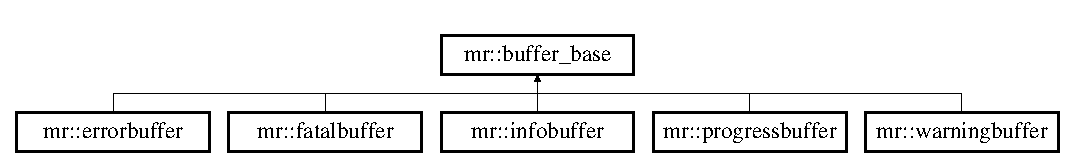
\includegraphics[height=1.80645cm]{structmr_1_1buffer__base}
\end{center}
\end{figure}
\subsection*{Public Member Functions}
\begin{CompactItemize}
\item 
{\bf buffer\_\-base} ()
\item 
virtual {\bf $\sim$buffer\_\-base} ()
\item 
virtual int {\bf sync} ()
\begin{CompactList}\small\item\em from basic\_\-streambuf, stl function used to sync stream \item\end{CompactList}\item 
virtual void {\bf print} (const char $\ast$const s)=0
\begin{CompactList}\small\item\em virtual function to print string out \item\end{CompactList}\end{CompactItemize}


\subsection{Constructor \& Destructor Documentation}
\index{mr::buffer_base@{mr::buffer\_\-base}!buffer_base@{buffer\_\-base}}
\index{buffer_base@{buffer\_\-base}!mr::buffer_base@{mr::buffer\_\-base}}
\subsubsection{\setlength{\rightskip}{0pt plus 5cm}mr::buffer\_\-base::buffer\_\-base ()\hspace{0.3cm}{\tt  [inline]}}\label{structmr_1_1buffer__base_a0}


\index{mr::buffer_base@{mr::buffer\_\-base}!~buffer_base@{$\sim$buffer\_\-base}}
\index{~buffer_base@{$\sim$buffer\_\-base}!mr::buffer_base@{mr::buffer\_\-base}}
\subsubsection{\setlength{\rightskip}{0pt plus 5cm}virtual mr::buffer\_\-base::$\sim${\bf buffer\_\-base} ()\hspace{0.3cm}{\tt  [inline, virtual]}}\label{structmr_1_1buffer__base_a1}




\subsection{Member Function Documentation}
\index{mr::buffer_base@{mr::buffer\_\-base}!print@{print}}
\index{print@{print}!mr::buffer_base@{mr::buffer\_\-base}}
\subsubsection{\setlength{\rightskip}{0pt plus 5cm}virtual void mr::buffer\_\-base::print (const char $\ast$const {\em s})\hspace{0.3cm}{\tt  [pure virtual]}}\label{structmr_1_1buffer__base_a3}


virtual function to print string out 



Implemented in {\bf mr::infobuffer} {\rm (p.\,\pageref{structmr_1_1infobuffer_a1})}, {\bf mr::warningbuffer} {\rm (p.\,\pageref{structmr_1_1warningbuffer_a1})}, {\bf mr::errorbuffer} {\rm (p.\,\pageref{structmr_1_1errorbuffer_a1})}, {\bf mr::fatalbuffer} {\rm (p.\,\pageref{structmr_1_1fatalbuffer_a1})}, and {\bf mr::progressbuffer} {\rm (p.\,\pageref{structmr_1_1progressbuffer_a1})}.\index{mr::buffer_base@{mr::buffer\_\-base}!sync@{sync}}
\index{sync@{sync}!mr::buffer_base@{mr::buffer\_\-base}}
\subsubsection{\setlength{\rightskip}{0pt plus 5cm}virtual int mr::buffer\_\-base::sync ()\hspace{0.3cm}{\tt  [virtual]}}\label{structmr_1_1buffer__base_a2}


from basic\_\-streambuf, stl function used to sync stream 



The documentation for this struct was generated from the following file:\begin{CompactItemize}
\item 
{\bf mr\-Stream.h}\end{CompactItemize}

\section{mr::distances::Chessboard Struct Reference}
\label{structmr_1_1distances_1_1Chessboard}\index{mr::distances::Chessboard@{mr::distances::Chessboard}}
Functor to calculate chessboard distance.  


{\tt \#include $<$mr\-Distances.h$>$}

Inheritance diagram for mr::distances::Chessboard::\begin{figure}[H]
\begin{center}
\leavevmode
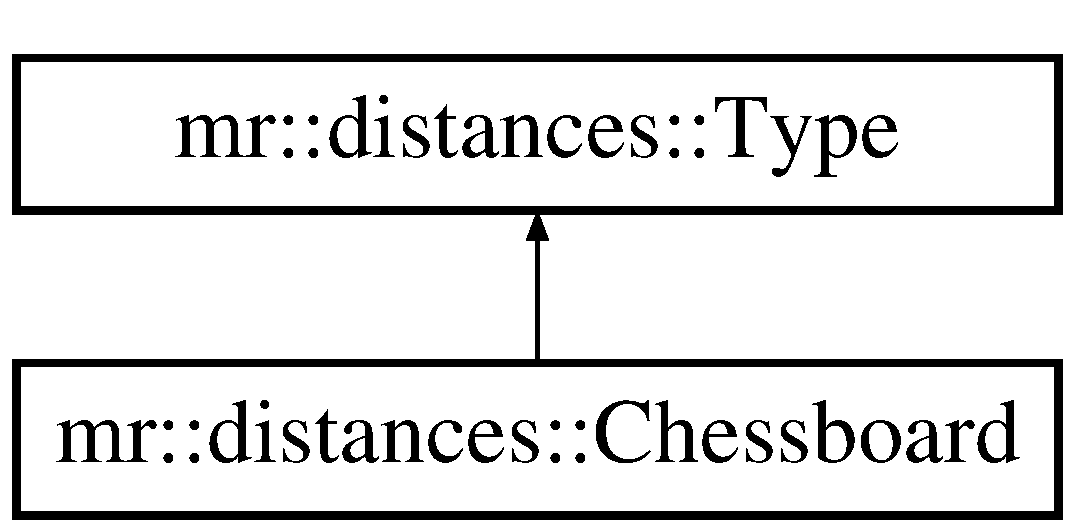
\includegraphics[height=2cm]{structmr_1_1distances_1_1Chessboard}
\end{center}
\end{figure}
\subsection*{Public Member Functions}
\begin{CompactItemize}
\item 
mi\-Scalar {\bf operator()} (const {\bf vector} \&d) const 
\item 
mi\-Scalar {\bf operator()} (const {\bf vector} \&d, const {\bf vector} \&s) const 
\end{CompactItemize}


\subsection{Detailed Description}
Functor to calculate chessboard distance. 



\subsection{Member Function Documentation}
\index{mr::distances::Chessboard@{mr::distances::Chessboard}!operator()@{operator()}}
\index{operator()@{operator()}!mr::distances::Chessboard@{mr::distances::Chessboard}}
\subsubsection{\setlength{\rightskip}{0pt plus 5cm}mi\-Scalar mr::distances::Chessboard::operator() (const {\bf vector} \& {\em d}, const {\bf vector} \& {\em s}) const\hspace{0.3cm}{\tt  [inline, virtual]}}\label{structmr_1_1distances_1_1Chessboard_a1}




Implements {\bf mr::distances::Type} {\rm (p.\,\pageref{structmr_1_1distances_1_1Type_a1})}.\index{mr::distances::Chessboard@{mr::distances::Chessboard}!operator()@{operator()}}
\index{operator()@{operator()}!mr::distances::Chessboard@{mr::distances::Chessboard}}
\subsubsection{\setlength{\rightskip}{0pt plus 5cm}mi\-Scalar mr::distances::Chessboard::operator() (const {\bf vector} \& {\em d}) const\hspace{0.3cm}{\tt  [inline, virtual]}}\label{structmr_1_1distances_1_1Chessboard_a0}




Implements {\bf mr::distances::Type} {\rm (p.\,\pageref{structmr_1_1distances_1_1Type_a0})}.

The documentation for this struct was generated from the following file:\begin{CompactItemize}
\item 
{\bf mr\-Distances.h}\end{CompactItemize}

\section{mr::color Struct Reference}
\label{structmr_1_1color}\index{mr::color@{mr::color}}
Define main color class that replaces mi\-Color.  


{\tt \#include $<$mr\-Color.h$>$}

\subsection*{Public Types}
\begin{CompactItemize}
\item 
typedef {\bf color} {\bf self}
\item 
typedef mi\-Scalar {\bf S}
\item 
enum {\bf space} \{ \par
{\bf k\-RGB} =  0, 
{\bf k\-HSV}, 
{\bf k\-HSL}, 
{\bf k\-XYZ}, 
\par
{\bf k\-CIEXYZ} =  k\-XYZ, 
{\bf k\-YPP}, 
{\bf k\-YCC}, 
{\bf k\-Unknown}
 \}
\end{CompactItemize}
\subsection*{Public Member Functions}
\begin{CompactItemize}
\item 
const mi\-Scalar {\bf Evaluate} (const unsigned short i) const 
\end{CompactItemize}
\begin{Indent}{\bf Color Space Conversion}\par
\begin{CompactItemize}
\item 
void {\bf xyz2rgb} ()
\begin{CompactList}\small\item\em Assuming color represents CIE XYZ, take it to RGB. \item\end{CompactList}\item 
void {\bf rgb2xyz} ()
\begin{CompactList}\small\item\em Assuming color represents RGB, take it to CIE XYZ. \item\end{CompactList}\item 
void {\bf hsv2rgb} ()
\begin{CompactList}\small\item\em Assuming color represents HSV, take it to RGB values. \item\end{CompactList}\item 
void {\bf rgb2hsv} ()
\begin{CompactList}\small\item\em Assuming color represents RGB, take it to HSV (r=H,g=S,b=V). \item\end{CompactList}\item 
void {\bf hsl2rgb} ()
\begin{CompactList}\small\item\em Assuming color represents HSL, take it to RGB values. \item\end{CompactList}\item 
void {\bf rgb2hsl} ()
\begin{CompactList}\small\item\em Assuming color represents RGB, take it to HSL (r=H,g=S,b=L). \item\end{CompactList}\item 
void {\bf ycc2rgb} ()
\begin{CompactList}\small\item\em Assuming color represents YCb\-Cr, take it to RGB values. \item\end{CompactList}\item 
void {\bf rgb2ycc} ()
\begin{CompactList}\small\item\em Assuming color represents RGB, take it to YCb\-Cr. \item\end{CompactList}\item 
void {\bf ypp2rgb} ()
\begin{CompactList}\small\item\em Assuming color represents YPb\-Pr, take it to RGB values. \item\end{CompactList}\item 
void {\bf rgb2ypp} ()
\begin{CompactList}\small\item\em Assuming color represents RGB, take it to YPb\-Pr. \item\end{CompactList}\item 
void {\bf to} (const {\bf space} to\-Space)
\begin{CompactList}\small\item\em Assume color is RGB, then take it to\-Space. \item\end{CompactList}\item 
void {\bf from} (const {\bf space} from\-Space)
\begin{CompactList}\small\item\em Assume color is defined in from\-Space, then take it to RGB. \item\end{CompactList}\item 
void {\bf transform} (const {\bf space} from\-Space, const {\bf space} to\-Space)
\begin{CompactList}\small\item\em Transform the color from one space to another. \item\end{CompactList}\end{CompactItemize}
\end{Indent}
\begin{Indent}{\bf Constructors}\par
\begin{CompactItemize}
\item 
template$<$class X, class Y, class Oper$>$ {\bf color} (const {\bf base::exp}$<$ X, Y, Oper $>$ \&e)
\item 
{\bf color} ({\bf k\-No\-Construct})
\item 
{\bf color} (const mi\-Color \&x)
\item 
{\bf color} (const mi\-Vector \&x, const mi\-Scalar aa=0.0f)
\begin{CompactList}\small\item\em Constructor to initialize from an mi\-Vector, with optional alpha. \item\end{CompactList}\item 
{\bf color} ()
\begin{CompactList}\small\item\em Default constructor. Sets r,g,b,a to 0. \item\end{CompactList}\item 
{\bf color} (const mi\-Scalar rgb, const mi\-Scalar aa=0.0f)
\item 
{\bf color} (const mi\-Scalar rr, const mi\-Scalar gg, const mi\-Scalar bb, const mi\-Scalar aa=0.0f)
\item 
{\bf color} (const {\bf space} t, const mi\-Color \&v)
\item 
{\bf color} (const {\bf space} t, const mi\-Scalar rr, const mi\-Scalar gg, const mi\-Scalar bb, const mi\-Scalar aa=0.0f)
\end{CompactItemize}
\end{Indent}
\begin{Indent}{\bf Copy Constructor}\par
\begin{CompactItemize}
\item 
{\bf color} (const {\bf color} \&x)
\end{CompactItemize}
\end{Indent}
\begin{Indent}{\bf Conversions}\par
\begin{CompactItemize}
\item 
{\bf operator mi\-Vector} ()
\begin{CompactList}\small\item\em Convert color to an mi\-Vector. \item\end{CompactList}\item 
{\bf operator vector} ()
\begin{CompactList}\small\item\em Convert color to a vector. \item\end{CompactList}\item 
{\bf operator point} ()
\begin{CompactList}\small\item\em Convert color to a point. \item\end{CompactList}\item 
{\bf operator normal} ()
\begin{CompactList}\small\item\em Convert color to a normal. \item\end{CompactList}\end{CompactItemize}
\end{Indent}
\begin{Indent}{\bf Assignment (With Alpha Channel)}\par
\begin{CompactItemize}
\item 
template$<$class X, class Y, class Oper$>$ const {\bf color} \& {\bf operator$|$=} (const {\bf base::exp}$<$ X, Y, Oper $>$ \&e)
\item 
const {\bf color} \& {\bf operator$|$=} (const {\bf color} \&x)
\item 
const {\bf color} \& {\bf operator$|$=} (const mi\-Color \&x)
\item 
const {\bf color} \& {\bf operator$|$=} (const mi\-Vector \&x)
\item 
const {\bf color} \& {\bf operator$|$=} (const mi\-Scalar rgba)
\end{CompactItemize}
\end{Indent}
\begin{Indent}{\bf Assignment (Without Alpha Channel)}\par
\begin{CompactItemize}
\item 
template$<$class X, class Y, class Oper$>$ const {\bf color} \& {\bf operator=} (const {\bf base::exp}$<$ X, Y, Oper $>$ \&e)
\item 
const {\bf color} \& {\bf operator=} (const {\bf color} \&x)
\item 
const {\bf color} \& {\bf operator=} (const mi\-Color \&x)
\item 
const {\bf color} \& {\bf operator=} (const mi\-Vector \&x)
\item 
const {\bf color} \& {\bf operator=} (const mi\-Scalar rgb)
\end{CompactItemize}
\end{Indent}
\begin{Indent}{\bf Swizzle operators}\par
\begin{CompactItemize}
\item 
const {\bf color} \& {\bf rgb} (const mi\-Color \&t)
\begin{CompactList}\small\item\em Set color to another mi\-Color. Original Alpha is not modified. \item\end{CompactList}\item 
const {\bf color} \& {\bf rgb} () const 
\begin{CompactList}\small\item\em Return color as {\bf rgb()}{\rm (p.\,\pageref{structmr_1_1color_z7_0})}. \item\end{CompactList}\item 
{\bf self} {\bf rrr} () const 
\begin{CompactList}\small\item\em 3 same channels \item\end{CompactList}\item 
{\bf self} {\bf ggg} () const 
\item 
{\bf self} {\bf bbb} () const 
\item 
{\bf self} {\bf aaa} () const 
\item 
{\bf self} {\bf brg} () const 
\item 
const {\bf self} \& {\bf brg} (const {\bf self} \&t)
\item 
{\bf self} {\bf gbr} () const 
\item 
const {\bf self} \& {\bf gbr} (const {\bf self} \&t)
\item 
{\bf self} {\bf rbg} () const 
\item 
const {\bf self} \& {\bf rbg} (const {\bf self} \&t)
\item 
{\bf self} {\bf bgr} () const 
\item 
const {\bf self} \& {\bf bgr} (const {\bf self} \&t)
\item 
{\bf self} {\bf grb} () const 
\item 
const {\bf self} \& {\bf grb} (const {\bf self} \&t)
\item 
{\bf self} {\bf rab} () const 
\item 
const {\bf self} \& {\bf rab} (const {\bf self} \&t)
\item 
{\bf self} {\bf rba} () const 
\item 
const {\bf self} \& {\bf rba} (const {\bf self} \&t)
\item 
{\bf self} {\bf bag} () const 
\item 
const {\bf self} \& {\bf bag} (const {\bf self} \&t)
\item 
{\bf self} {\bf gar} () const 
\item 
const {\bf self} \& {\bf gar} (const {\bf self} \&t)
\item 
{\bf self} {\bf rag} () const 
\item 
const {\bf self} \& {\bf rag} (const {\bf self} \&t)
\item 
{\bf self} {\bf bga} () const 
\item 
const {\bf self} \& {\bf bga} (const {\bf self} \&t)
\item 
{\bf self} {\bf gra} () const 
\item 
const {\bf self} \& {\bf gra} (const {\bf self} \&t)
\item 
{\bf self} {\bf rga} () const 
\item 
const {\bf self} \& {\bf rga} (const {\bf self} \&t)
\item 
{\bf self} {\bf grr} () const 
\item 
{\bf self} {\bf brr} () const 
\item 
{\bf self} {\bf arr} () const 
\item 
{\bf self} {\bf rgr} () const 
\item 
{\bf self} {\bf rbr} () const 
\item 
{\bf self} {\bf rar} () const 
\item 
{\bf self} {\bf rrg} () const 
\item 
{\bf self} {\bf rrb} () const 
\item 
{\bf self} {\bf rra} () const 
\item 
{\bf self} {\bf rgg} () const 
\item 
{\bf self} {\bf bgg} () const 
\item 
{\bf self} {\bf agg} () const 
\item 
{\bf self} {\bf grg} () const 
\item 
{\bf self} {\bf gbg} () const 
\item 
{\bf self} {\bf gag} () const 
\item 
{\bf self} {\bf ggr} () const 
\item 
{\bf self} {\bf ggb} () const 
\item 
{\bf self} {\bf gga} () const 
\item 
{\bf self} {\bf gbb} () const 
\item 
{\bf self} {\bf rbb} () const 
\item 
{\bf self} {\bf abb} () const 
\item 
{\bf self} {\bf bgb} () const 
\item 
{\bf self} {\bf brb} () const 
\item 
{\bf self} {\bf bab} () const 
\item 
{\bf self} {\bf bbg} () const 
\item 
{\bf self} {\bf bbr} () const 
\item 
{\bf self} {\bf bba} () const 
\item 
{\bf color} {\bf rrrr} ()
\item 
{\bf color} {\bf gggg} ()
\item 
{\bf color} {\bf bbbb} ()
\item 
{\bf color} {\bf aaaa} ()
\item 
{\bf color} {\bf rgba} ()
\item 
const {\bf self} \& {\bf rgba} (const mi\-Color \&t)
\item 
{\bf color} {\bf rgab} ()
\item 
const {\bf self} \& {\bf rgab} (const mi\-Color \&t)
\item 
{\bf color} {\bf rbga} ()
\item 
const {\bf self} \& {\bf rbga} (const mi\-Color \&t)
\item 
{\bf color} {\bf rbag} ()
\item 
const {\bf self} \& {\bf rbag} (const mi\-Color \&t)
\item 
{\bf color} {\bf rabg} ()
\item 
const {\bf self} \& {\bf rabg} (const mi\-Color \&t)
\item 
{\bf color} {\bf ragb} ()
\item 
const {\bf self} \& {\bf ragb} (const mi\-Color \&t)
\item 
{\bf color} {\bf rrgb} ()
\item 
{\bf color} {\bf rrbg} ()
\item 
{\bf color} {\bf rrag} ()
\item 
{\bf color} {\bf rrga} ()
\item 
{\bf color} {\bf rrab} ()
\item 
{\bf color} {\bf rrba} ()
\item 
{\bf color} {\bf grrb} ()
\item 
{\bf color} {\bf brrg} ()
\item 
{\bf color} {\bf grra} ()
\item 
{\bf color} {\bf arrg} ()
\item 
{\bf color} {\bf brra} ()
\item 
{\bf color} {\bf arrb} ()
\item 
{\bf color} {\bf gbrr} ()
\item 
{\bf color} {\bf bgrr} ()
\item 
{\bf color} {\bf abrr} ()
\item 
{\bf color} {\bf barr} ()
\item 
{\bf color} {\bf agrr} ()
\item 
{\bf color} {\bf garr} ()
\item 
{\bf color} {\bf rrrg} ()
\item 
{\bf color} {\bf rrrb} ()
\item 
{\bf color} {\bf rrra} ()
\item 
{\bf color} {\bf rrgr} ()
\item 
{\bf color} {\bf rrbr} ()
\item 
{\bf color} {\bf rrar} ()
\item 
{\bf color} {\bf rgrr} ()
\item 
{\bf color} {\bf rbrr} ()
\item 
{\bf color} {\bf rarr} ()
\item 
{\bf color} {\bf grrr} ()
\item 
{\bf color} {\bf brrr} ()
\item 
{\bf color} {\bf arrr} ()
\item 
{\bf color} {\bf grba} ()
\item 
const {\bf self} \& {\bf grba} (const mi\-Color \&t)
\item 
{\bf color} {\bf grab} ()
\item 
const {\bf self} \& {\bf grab} (const mi\-Color \&t)
\item 
{\bf color} {\bf gbra} ()
\item 
const {\bf self} \& {\bf gbra} (const mi\-Color \&t)
\item 
{\bf color} {\bf gbar} ()
\item 
const {\bf self} \& {\bf gbar} (const mi\-Color \&t)
\item 
{\bf color} {\bf gabr} ()
\item 
const {\bf self} \& {\bf gabr} (const mi\-Color \&t)
\item 
{\bf color} {\bf garb} ()
\item 
const {\bf self} \& {\bf garb} (const mi\-Color \&t)
\item 
{\bf color} {\bf ggrb} ()
\item 
{\bf color} {\bf ggbr} ()
\item 
{\bf color} {\bf ggar} ()
\item 
{\bf color} {\bf ggra} ()
\item 
{\bf color} {\bf ggab} ()
\item 
{\bf color} {\bf ggba} ()
\item 
{\bf color} {\bf rggb} ()
\item 
{\bf color} {\bf bggr} ()
\item 
{\bf color} {\bf rgga} ()
\item 
{\bf color} {\bf aggr} ()
\item 
{\bf color} {\bf bgga} ()
\item 
{\bf color} {\bf aggb} ()
\item 
{\bf color} {\bf rbgg} ()
\item 
{\bf color} {\bf brgg} ()
\item 
{\bf color} {\bf abgg} ()
\item 
{\bf color} {\bf bagg} ()
\item 
{\bf color} {\bf argg} ()
\item 
{\bf color} {\bf ragg} ()
\item 
{\bf color} {\bf gggr} ()
\item 
{\bf color} {\bf gggb} ()
\item 
{\bf color} {\bf ggga} ()
\item 
{\bf color} {\bf ggrg} ()
\item 
{\bf color} {\bf ggbg} ()
\item 
{\bf color} {\bf ggag} ()
\item 
{\bf color} {\bf grgg} ()
\item 
{\bf color} {\bf gbgg} ()
\item 
{\bf color} {\bf gagg} ()
\item 
{\bf color} {\bf rggg} ()
\item 
{\bf color} {\bf bggg} ()
\item 
{\bf color} {\bf aggg} ()
\item 
{\bf color} {\bf bgra} ()
\item 
const {\bf self} \& {\bf bgra} (const mi\-Color \&t)
\item 
{\bf color} {\bf bgar} ()
\item 
const {\bf self} \& {\bf bgar} (const mi\-Color \&t)
\item 
{\bf color} {\bf brga} ()
\item 
const {\bf self} \& {\bf brga} (const mi\-Color \&t)
\item 
{\bf color} {\bf brag} ()
\item 
const {\bf self} \& {\bf brag} (const mi\-Color \&t)
\item 
{\bf color} {\bf barg} ()
\item 
const {\bf self} \& {\bf barg} (const mi\-Color \&t)
\item 
{\bf color} {\bf bagr} ()
\item 
const {\bf self} \& {\bf bagr} (const mi\-Color \&t)
\item 
{\bf color} {\bf bbgr} ()
\item 
{\bf color} {\bf bbrg} ()
\item 
{\bf color} {\bf bbag} ()
\item 
{\bf color} {\bf bbga} ()
\item 
{\bf color} {\bf bbar} ()
\item 
{\bf color} {\bf bbra} ()
\item 
{\bf color} {\bf gbbr} ()
\item 
{\bf color} {\bf rbbg} ()
\item 
{\bf color} {\bf gbba} ()
\item 
{\bf color} {\bf abbg} ()
\item 
{\bf color} {\bf rbba} ()
\item 
{\bf color} {\bf abbr} ()
\item 
{\bf color} {\bf grbb} ()
\item 
{\bf color} {\bf rgbb} ()
\item 
{\bf color} {\bf arbb} ()
\item 
{\bf color} {\bf rabb} ()
\item 
{\bf color} {\bf agbb} ()
\item 
{\bf color} {\bf gabb} ()
\item 
{\bf color} {\bf bbbg} ()
\item 
{\bf color} {\bf bbbr} ()
\item 
{\bf color} {\bf bbba} ()
\item 
{\bf color} {\bf bbgb} ()
\item 
{\bf color} {\bf bbrb} ()
\item 
{\bf color} {\bf bbab} ()
\item 
{\bf color} {\bf bgbb} ()
\item 
{\bf color} {\bf brbb} ()
\item 
{\bf color} {\bf babb} ()
\item 
{\bf color} {\bf gbbb} ()
\item 
{\bf color} {\bf rbbb} ()
\item 
{\bf color} {\bf abbb} ()
\item 
{\bf color} {\bf agbr} ()
\item 
const {\bf self} \& {\bf agbr} (const mi\-Color \&t)
\item 
{\bf color} {\bf agrb} ()
\item 
const {\bf self} \& {\bf agrb} (const mi\-Color \&t)
\item 
{\bf color} {\bf abgr} ()
\item 
const {\bf self} \& {\bf abgr} (const mi\-Color \&t)
\item 
{\bf color} {\bf abrg} ()
\item 
const {\bf self} \& {\bf abrg} (const mi\-Color \&t)
\item 
{\bf color} {\bf arbg} ()
\item 
const {\bf self} \& {\bf arbg} (const mi\-Color \&t)
\item 
{\bf color} {\bf argb} ()
\item 
const {\bf self} \& {\bf argb} (const mi\-Color \&t)
\item 
{\bf color} {\bf aagb} ()
\item 
{\bf color} {\bf aabg} ()
\item 
{\bf color} {\bf aarg} ()
\item 
{\bf color} {\bf aagr} ()
\item 
{\bf color} {\bf aarb} ()
\item 
{\bf color} {\bf aabr} ()
\item 
{\bf color} {\bf gaab} ()
\item 
{\bf color} {\bf baag} ()
\item 
{\bf color} {\bf gaar} ()
\item 
{\bf color} {\bf raag} ()
\item 
{\bf color} {\bf baar} ()
\item 
{\bf color} {\bf raab} ()
\item 
{\bf color} {\bf gbaa} ()
\item 
{\bf color} {\bf bgaa} ()
\item 
{\bf color} {\bf rbaa} ()
\item 
{\bf color} {\bf braa} ()
\item 
{\bf color} {\bf rgaa} ()
\item 
{\bf color} {\bf graa} ()
\item 
{\bf color} {\bf aaag} ()
\item 
{\bf color} {\bf aaab} ()
\item 
{\bf color} {\bf aaar} ()
\item 
{\bf color} {\bf aaga} ()
\item 
{\bf color} {\bf aaba} ()
\item 
{\bf color} {\bf aara} ()
\item 
{\bf color} {\bf agaa} ()
\item 
{\bf color} {\bf abaa} ()
\item 
{\bf color} {\bf araa} ()
\item 
{\bf color} {\bf gaaa} ()
\item 
{\bf color} {\bf baaa} ()
\item 
{\bf color} {\bf raaa} ()
\end{CompactItemize}
\end{Indent}
\begin{Indent}{\bf Debugging (only active if MR\_\-DEBUG is defined)}\par
\begin{CompactItemize}
\item 
void {\bf is\-Valid} () const 
\begin{CompactList}\small\item\em mr\-ASSERT color is valid (ie. is Positive) \item\end{CompactList}\item 
void {\bf is\-In\-Range} () const 
\begin{CompactList}\small\item\em mr\-ASSERT all the rgba channel values are in range [0,1] \item\end{CompactList}\item 
void {\bf is\-Positive} () const 
\begin{CompactList}\small\item\em mr\-ASSERT all the rgba channel values are positive numbers (or 0) \item\end{CompactList}\item 
void {\bf is\-Premult} () const 
\end{CompactItemize}
\end{Indent}
\begin{Indent}{\bf Indexed Component Access}\par
\begin{CompactItemize}
\item 
mi\-Scalar \& {\bf operator[$\,$]} (const unsigned short i)
\begin{CompactList}\small\item\em Component setter using [0,3] index. \item\end{CompactList}\item 
const mi\-Scalar {\bf operator[$\,$]} (const unsigned short i) const 
\begin{CompactList}\small\item\em Component access using [0,3] index. \item\end{CompactList}\end{CompactItemize}
\end{Indent}
\begin{Indent}{\bf Equality}\par
\begin{CompactItemize}
\item 
template$<$class X, class Y, class Oper$>$ const bool {\bf operator==} (const {\bf base::exp}$<$ X, Y, Oper $>$ \&e) const 
\item 
const bool {\bf operator==} (const mi\-Color \&x) const 
\item 
const bool {\bf operator==} (const mi\-Scalar x) const 
\item 
template$<$class X, class Y, class Oper$>$ const bool {\bf operator!=} (const {\bf base::exp}$<$ X, Y, Oper $>$ \&e) const 
\item 
const bool {\bf operator!=} (const mi\-Color \&x) const 
\item 
const bool {\bf operator!=} (const mi\-Scalar x) const 
\end{CompactItemize}
\end{Indent}
\begin{Indent}{\bf RGB Luminance Comparisons}\par
\begin{CompactItemize}
\item 
bool {\bf operator$<$} (const mi\-Scalar a) const 
\begin{CompactList}\small\item\em Compare R+G+B $<$ Scalar. \item\end{CompactList}\item 
bool {\bf operator$>$} (const mi\-Scalar a) const 
\begin{CompactList}\small\item\em Compare R+G+B $>$ Scalar. \item\end{CompactList}\item 
bool {\bf operator$<$=} (const mi\-Scalar a) const 
\begin{CompactList}\small\item\em Compare R+G+B $<$= Scalar. \item\end{CompactList}\item 
bool {\bf operator$>$=} (const mi\-Scalar a) const 
\begin{CompactList}\small\item\em Compare R+G+B $>$= Scalar. \item\end{CompactList}\item 
bool {\bf operator$<$} (const mi\-Color \&a) const 
\begin{CompactList}\small\item\em Compare R+G+B $<$ R+G+B of other color. \item\end{CompactList}\item 
bool {\bf operator$>$} (const mi\-Color \&a) const 
\begin{CompactList}\small\item\em Compare R+G+B $>$ R+G+B of other color. \item\end{CompactList}\item 
bool {\bf operator$<$=} (const mi\-Color \&a) const 
\begin{CompactList}\small\item\em Compare R+G+B $<$= R+G+B of other color. \item\end{CompactList}\item 
bool {\bf operator$>$=} (const mi\-Color \&a) const 
\begin{CompactList}\small\item\em Compare R+G+B $>$= R+G+B of other color. \item\end{CompactList}\end{CompactItemize}
\end{Indent}
\begin{Indent}{\bf Per channel comparisons}\par
\begin{CompactItemize}
\item 
{\bf color} {\bf less\-Than} (const mi\-Color \&b)
\item 
{\bf color} {\bf less\-Than\-Equal} (const mi\-Color \&b)
\item 
{\bf color} {\bf greater\-Than} (const mi\-Color \&b)
\item 
{\bf color} {\bf greater\-Than\-Equal} (const mi\-Color \&b)
\item 
const bool {\bf any} ()
\item 
const bool {\bf any\_\-rgb} ()
\end{CompactItemize}
\end{Indent}
\begin{Indent}{\bf Operators}\par
\begin{CompactItemize}
\item 
{\bf color} {\bf operator-} () const 
\begin{CompactList}\small\item\em Per component negation. Original Alpha is NOT modified. \item\end{CompactList}\item 
template$<$class X, class Y, class Oper$>$ const {\bf color} \& {\bf operator+=} (const {\bf base::exp}$<$ X, Y, Oper $>$ \&t)
\item 
const {\bf color} \& {\bf operator+=} (const mi\-Scalar \&x)
\item 
const {\bf color} \& {\bf operator+=} (const mi\-Color \&x)
\item 
template$<$class X, class Y, class Oper$>$ const {\bf color} \& {\bf operator-=} (const {\bf base::exp}$<$ X, Y, Oper $>$ \&b)
\item 
const {\bf color} \& {\bf operator-=} (const mi\-Scalar x)
\item 
const {\bf color} \& {\bf operator-=} (const mi\-Color \&x)
\item 
template$<$class X, class Y, class Oper$>$ const {\bf color} \& {\bf operator $\ast$=} (const {\bf base::exp}$<$ X, Y, Oper $>$ \&b)
\item 
const {\bf color} \& {\bf operator $\ast$=} (const mi\-Scalar x)
\item 
const {\bf color} \& {\bf operator $\ast$=} (const mi\-Color \&x)
\item 
template$<$class X, class Y, class Oper$>$ const {\bf color} \& {\bf operator/=} (const {\bf base::exp}$<$ X, Y, Oper $>$ \&b)
\item 
const {\bf color} \& {\bf operator/=} (const mi\-Scalar x)
\item 
const {\bf color} \& {\bf operator/=} (const mi\-Color \&x)
\end{CompactItemize}
\end{Indent}
\begin{Indent}{\bf Common functions on colors}\par
\begin{CompactItemize}
\item 
bool {\bf is\-Equivalent} (const mi\-Color \&x, const mi\-Scalar tolerance=mi\-SCALAR\_\-EPSILON) const 
\begin{CompactList}\small\item\em Verify two colors are equivalent up to a certain tolerance. \item\end{CompactList}\item 
const {\bf color} \& {\bf mix} (const mi\-Color \&x, const mi\-Scalar p)
\item 
const {\bf color} \& {\bf clamp} (const mi\-Color \&a, const mi\-Color \&b)
\begin{CompactList}\small\item\em Clamp color to this min/max values. \item\end{CompactList}\item 
const {\bf color} \& {\bf clamp} (const mi\-Scalar a, const mi\-Scalar b)
\begin{CompactList}\small\item\em Clamp color to this min/max values. \item\end{CompactList}\item 
const {\bf color} \& {\bf clamp} (const mi\-Color \&a, const mi\-Scalar b)
\begin{CompactList}\small\item\em Clamp color to this min/max values. \item\end{CompactList}\item 
const {\bf color} \& {\bf clamp} (const mi\-Scalar a, const mi\-Color \&b)
\begin{CompactList}\small\item\em Clamp color to this min/max values. \item\end{CompactList}\end{CompactItemize}
\end{Indent}
\begin{Indent}{\bf Color Correction}\par
\begin{CompactItemize}
\item 
void {\bf gamma} (const mi\-Scalar p)
\begin{CompactList}\small\item\em Control gamma ( a pow() function ). \item\end{CompactList}\item 
mi\-Scalar {\bf lumma} (const mi\-State $\ast$state)
\begin{CompactList}\small\item\em Returns lumma of color (using state-$>$options-$>$luminance). \item\end{CompactList}\item 
void {\bf saturation} (const mi\-State $\ast$state, const mi\-Scalar p)
\end{CompactItemize}
\end{Indent}


\subsection{Detailed Description}
Define main color class that replaces mi\-Color. 



\subsection{Member Typedef Documentation}
\index{mr::color@{mr::color}!S@{S}}
\index{S@{S}!mr::color@{mr::color}}
\subsubsection{\setlength{\rightskip}{0pt plus 5cm}typedef mi\-Scalar {\bf mr::color::S}}\label{structmr_1_1color_w1}


\index{mr::color@{mr::color}!self@{self}}
\index{self@{self}!mr::color@{mr::color}}
\subsubsection{\setlength{\rightskip}{0pt plus 5cm}typedef {\bf color} {\bf mr::color::self}}\label{structmr_1_1color_w0}




\subsection{Member Enumeration Documentation}
\index{mr::color@{mr::color}!space@{space}}
\index{space@{space}!mr::color@{mr::color}}
\subsubsection{\setlength{\rightskip}{0pt plus 5cm}enum {\bf mr::color::space}}\label{structmr_1_1color_w10}


color spaces \begin{Desc}
\item[{\bf Todo}]add other spaces:\end{Desc}
\begin{Desc}
\item[Enumeration values: ]\par
\begin{description}
\index{kRGB@{kRGB}!mr::color@{mr::color}}\index{mr::color@{mr::color}!kRGB@{kRGB}}\item[{\em 
k\-RGB\label{structmr_1_1color_w10w2}
}]\index{kHSV@{kHSV}!mr::color@{mr::color}}\index{mr::color@{mr::color}!kHSV@{kHSV}}\item[{\em 
k\-HSV\label{structmr_1_1color_w10w3}
}]\index{kHSL@{kHSL}!mr::color@{mr::color}}\index{mr::color@{mr::color}!kHSL@{kHSL}}\item[{\em 
k\-HSL\label{structmr_1_1color_w10w4}
}]\index{kXYZ@{kXYZ}!mr::color@{mr::color}}\index{mr::color@{mr::color}!kXYZ@{kXYZ}}\item[{\em 
k\-XYZ\label{structmr_1_1color_w10w5}
}]\index{kCIEXYZ@{kCIEXYZ}!mr::color@{mr::color}}\index{mr::color@{mr::color}!kCIEXYZ@{kCIEXYZ}}\item[{\em 
k\-CIEXYZ\label{structmr_1_1color_w10w6}
}]\index{kYPP@{kYPP}!mr::color@{mr::color}}\index{mr::color@{mr::color}!kYPP@{kYPP}}\item[{\em 
k\-YPP\label{structmr_1_1color_w10w7}
}]\index{kYCC@{kYCC}!mr::color@{mr::color}}\index{mr::color@{mr::color}!kYCC@{kYCC}}\item[{\em 
k\-YCC\label{structmr_1_1color_w10w8}
}]\index{kUnknown@{kUnknown}!mr::color@{mr::color}}\index{mr::color@{mr::color}!kUnknown@{kUnknown}}\item[{\em 
k\-Unknown\label{structmr_1_1color_w10w9}
}]\end{description}
\end{Desc}



\subsection{Constructor \& Destructor Documentation}
\index{mr::color@{mr::color}!color@{color}}
\index{color@{color}!mr::color@{mr::color}}
\subsubsection{\setlength{\rightskip}{0pt plus 5cm}template$<$class X, class Y, class Oper$>$ mr::color::color (const {\bf base::exp}$<$ X, Y, Oper $>$ \& {\em e})\hspace{0.3cm}{\tt  [inline]}}\label{structmr_1_1color_z1_0}


Constructor to evaluate an expression (such as a concatenation of operations) \index{mr::color@{mr::color}!color@{color}}
\index{color@{color}!mr::color@{mr::color}}
\subsubsection{\setlength{\rightskip}{0pt plus 5cm}mr::color::color ({\bf k\-No\-Construct})\hspace{0.3cm}{\tt  [inline]}}\label{structmr_1_1color_z1_1}


Quick constructor. r,g,b,a values remain undefined and should later be set. \index{mr::color@{mr::color}!color@{color}}
\index{color@{color}!mr::color@{mr::color}}
\subsubsection{\setlength{\rightskip}{0pt plus 5cm}mr::color::color (const mi\-Color \& {\em x})\hspace{0.3cm}{\tt  [inline]}}\label{structmr_1_1color_z1_2}


Constructor to initialize from an mi\-Color. Note that alpha channel is also changed. \index{mr::color@{mr::color}!color@{color}}
\index{color@{color}!mr::color@{mr::color}}
\subsubsection{\setlength{\rightskip}{0pt plus 5cm}mr::color::color (const mi\-Vector \& {\em x}, const mi\-Scalar {\em aa} = 0.0f)\hspace{0.3cm}{\tt  [inline]}}\label{structmr_1_1color_z1_3}


Constructor to initialize from an mi\-Vector, with optional alpha. 

\index{mr::color@{mr::color}!color@{color}}
\index{color@{color}!mr::color@{mr::color}}
\subsubsection{\setlength{\rightskip}{0pt plus 5cm}mr::color::color ()\hspace{0.3cm}{\tt  [inline]}}\label{structmr_1_1color_z1_4}


Default constructor. Sets r,g,b,a to 0. 

\index{mr::color@{mr::color}!color@{color}}
\index{color@{color}!mr::color@{mr::color}}
\subsubsection{\setlength{\rightskip}{0pt plus 5cm}mr::color::color (const mi\-Scalar {\em rgb}, const mi\-Scalar {\em aa} = 0.0f)\hspace{0.3cm}{\tt  [inline]}}\label{structmr_1_1color_z1_5}


Constructor to initialize rgb channels from a mi\-Scalar, with optional alpha \index{mr::color@{mr::color}!color@{color}}
\index{color@{color}!mr::color@{mr::color}}
\subsubsection{\setlength{\rightskip}{0pt plus 5cm}mr::color::color (const mi\-Scalar {\em rr}, const mi\-Scalar {\em gg}, const mi\-Scalar {\em bb}, const mi\-Scalar {\em aa} = 0.0f)\hspace{0.3cm}{\tt  [inline]}}\label{structmr_1_1color_z1_6}


Constructor to initialize each rgb channel individually, with optional alpha \index{mr::color@{mr::color}!color@{color}}
\index{color@{color}!mr::color@{mr::color}}
\subsubsection{\setlength{\rightskip}{0pt plus 5cm}mr::color::color (const {\bf space} {\em t}, const mi\-Color \& {\em v})\hspace{0.3cm}{\tt  [inline]}}\label{structmr_1_1color_z1_7}


Constructor to initialize from an mi\-Color, but assuming the color passed is in a particular color space. The new color created is defined in rgb and is equivalent to the color passed to it. Note that alpha channel is also changed. This is a similar construct to renderman's: color x = color \char`\"{}hsv\char`\"{} (1,0,0); \index{mr::color@{mr::color}!color@{color}}
\index{color@{color}!mr::color@{mr::color}}
\subsubsection{\setlength{\rightskip}{0pt plus 5cm}mr::color::color (const {\bf space} {\em t}, const mi\-Scalar {\em rr}, const mi\-Scalar {\em gg}, const mi\-Scalar {\em bb}, const mi\-Scalar {\em aa} = 0.0f)\hspace{0.3cm}{\tt  [inline]}}\label{structmr_1_1color_z1_8}


Constructor to initialize each channel individually, but assuming the values passed are in a particular color space. The new color created is defined in rgb and is equivalent to the color passed to it. \index{mr::color@{mr::color}!color@{color}}
\index{color@{color}!mr::color@{mr::color}}
\subsubsection{\setlength{\rightskip}{0pt plus 5cm}mr::color::color (const {\bf color} \& {\em x})\hspace{0.3cm}{\tt  [inline]}}\label{structmr_1_1color_z2_0}




\subsection{Member Function Documentation}
\index{mr::color@{mr::color}!aaa@{aaa}}
\index{aaa@{aaa}!mr::color@{mr::color}}
\subsubsection{\setlength{\rightskip}{0pt plus 5cm}{\bf self} mr::color::aaa () const\hspace{0.3cm}{\tt  [inline]}}\label{structmr_1_1color_z7_5}


\index{mr::color@{mr::color}!aaaa@{aaaa}}
\index{aaaa@{aaaa}!mr::color@{mr::color}}
\subsubsection{\setlength{\rightskip}{0pt plus 5cm}{\bf color} mr::color::aaaa ()\hspace{0.3cm}{\tt  [inline]}}\label{structmr_1_1color_z7_62}


\index{mr::color@{mr::color}!aaab@{aaab}}
\index{aaab@{aaab}!mr::color@{mr::color}}
\subsubsection{\setlength{\rightskip}{0pt plus 5cm}{\bf color} mr::color::aaab ()\hspace{0.3cm}{\tt  [inline]}}\label{structmr_1_1color_z7_220}


\index{mr::color@{mr::color}!aaag@{aaag}}
\index{aaag@{aaag}!mr::color@{mr::color}}
\subsubsection{\setlength{\rightskip}{0pt plus 5cm}{\bf color} mr::color::aaag ()\hspace{0.3cm}{\tt  [inline]}}\label{structmr_1_1color_z7_219}


\index{mr::color@{mr::color}!aaar@{aaar}}
\index{aaar@{aaar}!mr::color@{mr::color}}
\subsubsection{\setlength{\rightskip}{0pt plus 5cm}{\bf color} mr::color::aaar ()\hspace{0.3cm}{\tt  [inline]}}\label{structmr_1_1color_z7_221}


\index{mr::color@{mr::color}!aaba@{aaba}}
\index{aaba@{aaba}!mr::color@{mr::color}}
\subsubsection{\setlength{\rightskip}{0pt plus 5cm}{\bf color} mr::color::aaba ()\hspace{0.3cm}{\tt  [inline]}}\label{structmr_1_1color_z7_223}


\index{mr::color@{mr::color}!aabg@{aabg}}
\index{aabg@{aabg}!mr::color@{mr::color}}
\subsubsection{\setlength{\rightskip}{0pt plus 5cm}{\bf color} mr::color::aabg ()\hspace{0.3cm}{\tt  [inline]}}\label{structmr_1_1color_z7_202}


\index{mr::color@{mr::color}!aabr@{aabr}}
\index{aabr@{aabr}!mr::color@{mr::color}}
\subsubsection{\setlength{\rightskip}{0pt plus 5cm}{\bf color} mr::color::aabr ()\hspace{0.3cm}{\tt  [inline]}}\label{structmr_1_1color_z7_206}


\index{mr::color@{mr::color}!aaga@{aaga}}
\index{aaga@{aaga}!mr::color@{mr::color}}
\subsubsection{\setlength{\rightskip}{0pt plus 5cm}{\bf color} mr::color::aaga ()\hspace{0.3cm}{\tt  [inline]}}\label{structmr_1_1color_z7_222}


\index{mr::color@{mr::color}!aagb@{aagb}}
\index{aagb@{aagb}!mr::color@{mr::color}}
\subsubsection{\setlength{\rightskip}{0pt plus 5cm}{\bf color} mr::color::aagb ()\hspace{0.3cm}{\tt  [inline]}}\label{structmr_1_1color_z7_201}


\index{mr::color@{mr::color}!aagr@{aagr}}
\index{aagr@{aagr}!mr::color@{mr::color}}
\subsubsection{\setlength{\rightskip}{0pt plus 5cm}{\bf color} mr::color::aagr ()\hspace{0.3cm}{\tt  [inline]}}\label{structmr_1_1color_z7_204}


\index{mr::color@{mr::color}!aara@{aara}}
\index{aara@{aara}!mr::color@{mr::color}}
\subsubsection{\setlength{\rightskip}{0pt plus 5cm}{\bf color} mr::color::aara ()\hspace{0.3cm}{\tt  [inline]}}\label{structmr_1_1color_z7_224}


\index{mr::color@{mr::color}!aarb@{aarb}}
\index{aarb@{aarb}!mr::color@{mr::color}}
\subsubsection{\setlength{\rightskip}{0pt plus 5cm}{\bf color} mr::color::aarb ()\hspace{0.3cm}{\tt  [inline]}}\label{structmr_1_1color_z7_205}


\index{mr::color@{mr::color}!aarg@{aarg}}
\index{aarg@{aarg}!mr::color@{mr::color}}
\subsubsection{\setlength{\rightskip}{0pt plus 5cm}{\bf color} mr::color::aarg ()\hspace{0.3cm}{\tt  [inline]}}\label{structmr_1_1color_z7_203}


\index{mr::color@{mr::color}!abaa@{abaa}}
\index{abaa@{abaa}!mr::color@{mr::color}}
\subsubsection{\setlength{\rightskip}{0pt plus 5cm}{\bf color} mr::color::abaa ()\hspace{0.3cm}{\tt  [inline]}}\label{structmr_1_1color_z7_226}


\index{mr::color@{mr::color}!abb@{abb}}
\index{abb@{abb}!mr::color@{mr::color}}
\subsubsection{\setlength{\rightskip}{0pt plus 5cm}{\bf self} mr::color::abb () const\hspace{0.3cm}{\tt  [inline]}}\label{structmr_1_1color_z7_52}


\index{mr::color@{mr::color}!abbb@{abbb}}
\index{abbb@{abbb}!mr::color@{mr::color}}
\subsubsection{\setlength{\rightskip}{0pt plus 5cm}{\bf color} mr::color::abbb ()\hspace{0.3cm}{\tt  [inline]}}\label{structmr_1_1color_z7_188}


\index{mr::color@{mr::color}!abbg@{abbg}}
\index{abbg@{abbg}!mr::color@{mr::color}}
\subsubsection{\setlength{\rightskip}{0pt plus 5cm}{\bf color} mr::color::abbg ()\hspace{0.3cm}{\tt  [inline]}}\label{structmr_1_1color_z7_168}


\index{mr::color@{mr::color}!abbr@{abbr}}
\index{abbr@{abbr}!mr::color@{mr::color}}
\subsubsection{\setlength{\rightskip}{0pt plus 5cm}{\bf color} mr::color::abbr ()\hspace{0.3cm}{\tt  [inline]}}\label{structmr_1_1color_z7_170}


\index{mr::color@{mr::color}!abgg@{abgg}}
\index{abgg@{abgg}!mr::color@{mr::color}}
\subsubsection{\setlength{\rightskip}{0pt plus 5cm}{\bf color} mr::color::abgg ()\hspace{0.3cm}{\tt  [inline]}}\label{structmr_1_1color_z7_131}


\index{mr::color@{mr::color}!abgr@{abgr}}
\index{abgr@{abgr}!mr::color@{mr::color}}
\subsubsection{\setlength{\rightskip}{0pt plus 5cm}const {\bf self}\& mr::color::abgr (const mi\-Color \& {\em t})\hspace{0.3cm}{\tt  [inline]}}\label{structmr_1_1color_z7_194}


\index{mr::color@{mr::color}!abgr@{abgr}}
\index{abgr@{abgr}!mr::color@{mr::color}}
\subsubsection{\setlength{\rightskip}{0pt plus 5cm}{\bf color} mr::color::abgr ()\hspace{0.3cm}{\tt  [inline]}}\label{structmr_1_1color_z7_193}


\index{mr::color@{mr::color}!abrg@{abrg}}
\index{abrg@{abrg}!mr::color@{mr::color}}
\subsubsection{\setlength{\rightskip}{0pt plus 5cm}const {\bf self}\& mr::color::abrg (const mi\-Color \& {\em t})\hspace{0.3cm}{\tt  [inline]}}\label{structmr_1_1color_z7_196}


\index{mr::color@{mr::color}!abrg@{abrg}}
\index{abrg@{abrg}!mr::color@{mr::color}}
\subsubsection{\setlength{\rightskip}{0pt plus 5cm}{\bf color} mr::color::abrg ()\hspace{0.3cm}{\tt  [inline]}}\label{structmr_1_1color_z7_195}


\index{mr::color@{mr::color}!abrr@{abrr}}
\index{abrr@{abrr}!mr::color@{mr::color}}
\subsubsection{\setlength{\rightskip}{0pt plus 5cm}{\bf color} mr::color::abrr ()\hspace{0.3cm}{\tt  [inline]}}\label{structmr_1_1color_z7_89}


\index{mr::color@{mr::color}!agaa@{agaa}}
\index{agaa@{agaa}!mr::color@{mr::color}}
\subsubsection{\setlength{\rightskip}{0pt plus 5cm}{\bf color} mr::color::agaa ()\hspace{0.3cm}{\tt  [inline]}}\label{structmr_1_1color_z7_225}


\index{mr::color@{mr::color}!agbb@{agbb}}
\index{agbb@{agbb}!mr::color@{mr::color}}
\subsubsection{\setlength{\rightskip}{0pt plus 5cm}{\bf color} mr::color::agbb ()\hspace{0.3cm}{\tt  [inline]}}\label{structmr_1_1color_z7_175}


\index{mr::color@{mr::color}!agbr@{agbr}}
\index{agbr@{agbr}!mr::color@{mr::color}}
\subsubsection{\setlength{\rightskip}{0pt plus 5cm}const {\bf self}\& mr::color::agbr (const mi\-Color \& {\em t})\hspace{0.3cm}{\tt  [inline]}}\label{structmr_1_1color_z7_190}


\index{mr::color@{mr::color}!agbr@{agbr}}
\index{agbr@{agbr}!mr::color@{mr::color}}
\subsubsection{\setlength{\rightskip}{0pt plus 5cm}{\bf color} mr::color::agbr ()\hspace{0.3cm}{\tt  [inline]}}\label{structmr_1_1color_z7_189}


\index{mr::color@{mr::color}!agg@{agg}}
\index{agg@{agg}!mr::color@{mr::color}}
\subsubsection{\setlength{\rightskip}{0pt plus 5cm}{\bf self} mr::color::agg () const\hspace{0.3cm}{\tt  [inline]}}\label{structmr_1_1color_z7_43}


\index{mr::color@{mr::color}!aggb@{aggb}}
\index{aggb@{aggb}!mr::color@{mr::color}}
\subsubsection{\setlength{\rightskip}{0pt plus 5cm}{\bf color} mr::color::aggb ()\hspace{0.3cm}{\tt  [inline]}}\label{structmr_1_1color_z7_128}


\index{mr::color@{mr::color}!aggg@{aggg}}
\index{aggg@{aggg}!mr::color@{mr::color}}
\subsubsection{\setlength{\rightskip}{0pt plus 5cm}{\bf color} mr::color::aggg ()\hspace{0.3cm}{\tt  [inline]}}\label{structmr_1_1color_z7_146}


\index{mr::color@{mr::color}!aggr@{aggr}}
\index{aggr@{aggr}!mr::color@{mr::color}}
\subsubsection{\setlength{\rightskip}{0pt plus 5cm}{\bf color} mr::color::aggr ()\hspace{0.3cm}{\tt  [inline]}}\label{structmr_1_1color_z7_126}


\index{mr::color@{mr::color}!agrb@{agrb}}
\index{agrb@{agrb}!mr::color@{mr::color}}
\subsubsection{\setlength{\rightskip}{0pt plus 5cm}const {\bf self}\& mr::color::agrb (const mi\-Color \& {\em t})\hspace{0.3cm}{\tt  [inline]}}\label{structmr_1_1color_z7_192}


\index{mr::color@{mr::color}!agrb@{agrb}}
\index{agrb@{agrb}!mr::color@{mr::color}}
\subsubsection{\setlength{\rightskip}{0pt plus 5cm}{\bf color} mr::color::agrb ()\hspace{0.3cm}{\tt  [inline]}}\label{structmr_1_1color_z7_191}


\index{mr::color@{mr::color}!agrr@{agrr}}
\index{agrr@{agrr}!mr::color@{mr::color}}
\subsubsection{\setlength{\rightskip}{0pt plus 5cm}{\bf color} mr::color::agrr ()\hspace{0.3cm}{\tt  [inline]}}\label{structmr_1_1color_z7_91}


\index{mr::color@{mr::color}!any@{any}}
\index{any@{any}!mr::color@{mr::color}}
\subsubsection{\setlength{\rightskip}{0pt plus 5cm}const bool mr::color::any ()\hspace{0.3cm}{\tt  [inline]}}\label{structmr_1_1color_z12_4}


Returns true if any rgba channel is not 0. To be used mainly with the return of the functions of per channel comparison. For example: 

\footnotesize\begin{verbatim}           if ( c1.lessThan( c2 ).any() ) {
              mr_info("some channel in c1 is less than c2.")
           }
\end{verbatim}
\normalsize
\index{mr::color@{mr::color}!any_rgb@{any\_\-rgb}}
\index{any_rgb@{any\_\-rgb}!mr::color@{mr::color}}
\subsubsection{\setlength{\rightskip}{0pt plus 5cm}const bool mr::color::any\_\-rgb ()\hspace{0.3cm}{\tt  [inline]}}\label{structmr_1_1color_z12_5}


Returns true if any rgb channel is not 0. Alpha is ignored. To be used mainly with the return of the functions of per channel comparison. For example: 

\footnotesize\begin{verbatim}           if ( c1.lessThan( c2 ).any_rgb() ) {
              mr_info("some rgb channel in c1 is less than c2.")
           }
\end{verbatim}
\normalsize
\index{mr::color@{mr::color}!araa@{araa}}
\index{araa@{araa}!mr::color@{mr::color}}
\subsubsection{\setlength{\rightskip}{0pt plus 5cm}{\bf color} mr::color::araa ()\hspace{0.3cm}{\tt  [inline]}}\label{structmr_1_1color_z7_227}


\index{mr::color@{mr::color}!arbb@{arbb}}
\index{arbb@{arbb}!mr::color@{mr::color}}
\subsubsection{\setlength{\rightskip}{0pt plus 5cm}{\bf color} mr::color::arbb ()\hspace{0.3cm}{\tt  [inline]}}\label{structmr_1_1color_z7_173}


\index{mr::color@{mr::color}!arbg@{arbg}}
\index{arbg@{arbg}!mr::color@{mr::color}}
\subsubsection{\setlength{\rightskip}{0pt plus 5cm}const {\bf self}\& mr::color::arbg (const mi\-Color \& {\em t})\hspace{0.3cm}{\tt  [inline]}}\label{structmr_1_1color_z7_198}


\index{mr::color@{mr::color}!arbg@{arbg}}
\index{arbg@{arbg}!mr::color@{mr::color}}
\subsubsection{\setlength{\rightskip}{0pt plus 5cm}{\bf color} mr::color::arbg ()\hspace{0.3cm}{\tt  [inline]}}\label{structmr_1_1color_z7_197}


\index{mr::color@{mr::color}!argb@{argb}}
\index{argb@{argb}!mr::color@{mr::color}}
\subsubsection{\setlength{\rightskip}{0pt plus 5cm}const {\bf self}\& mr::color::argb (const mi\-Color \& {\em t})\hspace{0.3cm}{\tt  [inline]}}\label{structmr_1_1color_z7_200}


\index{mr::color@{mr::color}!argb@{argb}}
\index{argb@{argb}!mr::color@{mr::color}}
\subsubsection{\setlength{\rightskip}{0pt plus 5cm}{\bf color} mr::color::argb ()\hspace{0.3cm}{\tt  [inline]}}\label{structmr_1_1color_z7_199}


\index{mr::color@{mr::color}!argg@{argg}}
\index{argg@{argg}!mr::color@{mr::color}}
\subsubsection{\setlength{\rightskip}{0pt plus 5cm}{\bf color} mr::color::argg ()\hspace{0.3cm}{\tt  [inline]}}\label{structmr_1_1color_z7_133}


\index{mr::color@{mr::color}!arr@{arr}}
\index{arr@{arr}!mr::color@{mr::color}}
\subsubsection{\setlength{\rightskip}{0pt plus 5cm}{\bf self} mr::color::arr () const\hspace{0.3cm}{\tt  [inline]}}\label{structmr_1_1color_z7_34}


\index{mr::color@{mr::color}!arrb@{arrb}}
\index{arrb@{arrb}!mr::color@{mr::color}}
\subsubsection{\setlength{\rightskip}{0pt plus 5cm}{\bf color} mr::color::arrb ()\hspace{0.3cm}{\tt  [inline]}}\label{structmr_1_1color_z7_86}


\index{mr::color@{mr::color}!arrg@{arrg}}
\index{arrg@{arrg}!mr::color@{mr::color}}
\subsubsection{\setlength{\rightskip}{0pt plus 5cm}{\bf color} mr::color::arrg ()\hspace{0.3cm}{\tt  [inline]}}\label{structmr_1_1color_z7_84}


\index{mr::color@{mr::color}!arrr@{arrr}}
\index{arrr@{arrr}!mr::color@{mr::color}}
\subsubsection{\setlength{\rightskip}{0pt plus 5cm}{\bf color} mr::color::arrr ()\hspace{0.3cm}{\tt  [inline]}}\label{structmr_1_1color_z7_104}


\index{mr::color@{mr::color}!baaa@{baaa}}
\index{baaa@{baaa}!mr::color@{mr::color}}
\subsubsection{\setlength{\rightskip}{0pt plus 5cm}{\bf color} mr::color::baaa ()\hspace{0.3cm}{\tt  [inline]}}\label{structmr_1_1color_z7_229}


\index{mr::color@{mr::color}!baag@{baag}}
\index{baag@{baag}!mr::color@{mr::color}}
\subsubsection{\setlength{\rightskip}{0pt plus 5cm}{\bf color} mr::color::baag ()\hspace{0.3cm}{\tt  [inline]}}\label{structmr_1_1color_z7_208}


\index{mr::color@{mr::color}!baar@{baar}}
\index{baar@{baar}!mr::color@{mr::color}}
\subsubsection{\setlength{\rightskip}{0pt plus 5cm}{\bf color} mr::color::baar ()\hspace{0.3cm}{\tt  [inline]}}\label{structmr_1_1color_z7_211}


\index{mr::color@{mr::color}!bab@{bab}}
\index{bab@{bab}!mr::color@{mr::color}}
\subsubsection{\setlength{\rightskip}{0pt plus 5cm}{\bf self} mr::color::bab () const\hspace{0.3cm}{\tt  [inline]}}\label{structmr_1_1color_z7_55}


\index{mr::color@{mr::color}!babb@{babb}}
\index{babb@{babb}!mr::color@{mr::color}}
\subsubsection{\setlength{\rightskip}{0pt plus 5cm}{\bf color} mr::color::babb ()\hspace{0.3cm}{\tt  [inline]}}\label{structmr_1_1color_z7_185}


\index{mr::color@{mr::color}!bag@{bag}}
\index{bag@{bag}!mr::color@{mr::color}}
\subsubsection{\setlength{\rightskip}{0pt plus 5cm}const {\bf self}\& mr::color::bag (const {\bf self} \& {\em t})\hspace{0.3cm}{\tt  [inline]}}\label{structmr_1_1color_z7_21}


\index{mr::color@{mr::color}!bag@{bag}}
\index{bag@{bag}!mr::color@{mr::color}}
\subsubsection{\setlength{\rightskip}{0pt plus 5cm}{\bf self} mr::color::bag () const\hspace{0.3cm}{\tt  [inline]}}\label{structmr_1_1color_z7_20}


\index{mr::color@{mr::color}!bagg@{bagg}}
\index{bagg@{bagg}!mr::color@{mr::color}}
\subsubsection{\setlength{\rightskip}{0pt plus 5cm}{\bf color} mr::color::bagg ()\hspace{0.3cm}{\tt  [inline]}}\label{structmr_1_1color_z7_132}


\index{mr::color@{mr::color}!bagr@{bagr}}
\index{bagr@{bagr}!mr::color@{mr::color}}
\subsubsection{\setlength{\rightskip}{0pt plus 5cm}const {\bf self}\& mr::color::bagr (const mi\-Color \& {\em t})\hspace{0.3cm}{\tt  [inline]}}\label{structmr_1_1color_z7_158}


\index{mr::color@{mr::color}!bagr@{bagr}}
\index{bagr@{bagr}!mr::color@{mr::color}}
\subsubsection{\setlength{\rightskip}{0pt plus 5cm}{\bf color} mr::color::bagr ()\hspace{0.3cm}{\tt  [inline]}}\label{structmr_1_1color_z7_157}


\index{mr::color@{mr::color}!barg@{barg}}
\index{barg@{barg}!mr::color@{mr::color}}
\subsubsection{\setlength{\rightskip}{0pt plus 5cm}const {\bf self}\& mr::color::barg (const mi\-Color \& {\em t})\hspace{0.3cm}{\tt  [inline]}}\label{structmr_1_1color_z7_156}


\index{mr::color@{mr::color}!barg@{barg}}
\index{barg@{barg}!mr::color@{mr::color}}
\subsubsection{\setlength{\rightskip}{0pt plus 5cm}{\bf color} mr::color::barg ()\hspace{0.3cm}{\tt  [inline]}}\label{structmr_1_1color_z7_155}


\index{mr::color@{mr::color}!barr@{barr}}
\index{barr@{barr}!mr::color@{mr::color}}
\subsubsection{\setlength{\rightskip}{0pt plus 5cm}{\bf color} mr::color::barr ()\hspace{0.3cm}{\tt  [inline]}}\label{structmr_1_1color_z7_90}


\index{mr::color@{mr::color}!bba@{bba}}
\index{bba@{bba}!mr::color@{mr::color}}
\subsubsection{\setlength{\rightskip}{0pt plus 5cm}{\bf self} mr::color::bba () const\hspace{0.3cm}{\tt  [inline]}}\label{structmr_1_1color_z7_58}


\index{mr::color@{mr::color}!bbab@{bbab}}
\index{bbab@{bbab}!mr::color@{mr::color}}
\subsubsection{\setlength{\rightskip}{0pt plus 5cm}{\bf color} mr::color::bbab ()\hspace{0.3cm}{\tt  [inline]}}\label{structmr_1_1color_z7_182}


\index{mr::color@{mr::color}!bbag@{bbag}}
\index{bbag@{bbag}!mr::color@{mr::color}}
\subsubsection{\setlength{\rightskip}{0pt plus 5cm}{\bf color} mr::color::bbag ()\hspace{0.3cm}{\tt  [inline]}}\label{structmr_1_1color_z7_161}


\index{mr::color@{mr::color}!bbar@{bbar}}
\index{bbar@{bbar}!mr::color@{mr::color}}
\subsubsection{\setlength{\rightskip}{0pt plus 5cm}{\bf color} mr::color::bbar ()\hspace{0.3cm}{\tt  [inline]}}\label{structmr_1_1color_z7_163}


\index{mr::color@{mr::color}!bbb@{bbb}}
\index{bbb@{bbb}!mr::color@{mr::color}}
\subsubsection{\setlength{\rightskip}{0pt plus 5cm}{\bf self} mr::color::bbb () const\hspace{0.3cm}{\tt  [inline]}}\label{structmr_1_1color_z7_4}


\index{mr::color@{mr::color}!bbba@{bbba}}
\index{bbba@{bbba}!mr::color@{mr::color}}
\subsubsection{\setlength{\rightskip}{0pt plus 5cm}{\bf color} mr::color::bbba ()\hspace{0.3cm}{\tt  [inline]}}\label{structmr_1_1color_z7_179}


\index{mr::color@{mr::color}!bbbb@{bbbb}}
\index{bbbb@{bbbb}!mr::color@{mr::color}}
\subsubsection{\setlength{\rightskip}{0pt plus 5cm}{\bf color} mr::color::bbbb ()\hspace{0.3cm}{\tt  [inline]}}\label{structmr_1_1color_z7_61}


\index{mr::color@{mr::color}!bbbg@{bbbg}}
\index{bbbg@{bbbg}!mr::color@{mr::color}}
\subsubsection{\setlength{\rightskip}{0pt plus 5cm}{\bf color} mr::color::bbbg ()\hspace{0.3cm}{\tt  [inline]}}\label{structmr_1_1color_z7_177}


\index{mr::color@{mr::color}!bbbr@{bbbr}}
\index{bbbr@{bbbr}!mr::color@{mr::color}}
\subsubsection{\setlength{\rightskip}{0pt plus 5cm}{\bf color} mr::color::bbbr ()\hspace{0.3cm}{\tt  [inline]}}\label{structmr_1_1color_z7_178}


\index{mr::color@{mr::color}!bbg@{bbg}}
\index{bbg@{bbg}!mr::color@{mr::color}}
\subsubsection{\setlength{\rightskip}{0pt plus 5cm}{\bf self} mr::color::bbg () const\hspace{0.3cm}{\tt  [inline]}}\label{structmr_1_1color_z7_56}


\index{mr::color@{mr::color}!bbga@{bbga}}
\index{bbga@{bbga}!mr::color@{mr::color}}
\subsubsection{\setlength{\rightskip}{0pt plus 5cm}{\bf color} mr::color::bbga ()\hspace{0.3cm}{\tt  [inline]}}\label{structmr_1_1color_z7_162}


\index{mr::color@{mr::color}!bbgb@{bbgb}}
\index{bbgb@{bbgb}!mr::color@{mr::color}}
\subsubsection{\setlength{\rightskip}{0pt plus 5cm}{\bf color} mr::color::bbgb ()\hspace{0.3cm}{\tt  [inline]}}\label{structmr_1_1color_z7_180}


\index{mr::color@{mr::color}!bbgr@{bbgr}}
\index{bbgr@{bbgr}!mr::color@{mr::color}}
\subsubsection{\setlength{\rightskip}{0pt plus 5cm}{\bf color} mr::color::bbgr ()\hspace{0.3cm}{\tt  [inline]}}\label{structmr_1_1color_z7_159}


\index{mr::color@{mr::color}!bbr@{bbr}}
\index{bbr@{bbr}!mr::color@{mr::color}}
\subsubsection{\setlength{\rightskip}{0pt plus 5cm}{\bf self} mr::color::bbr () const\hspace{0.3cm}{\tt  [inline]}}\label{structmr_1_1color_z7_57}


\index{mr::color@{mr::color}!bbra@{bbra}}
\index{bbra@{bbra}!mr::color@{mr::color}}
\subsubsection{\setlength{\rightskip}{0pt plus 5cm}{\bf color} mr::color::bbra ()\hspace{0.3cm}{\tt  [inline]}}\label{structmr_1_1color_z7_164}


\index{mr::color@{mr::color}!bbrb@{bbrb}}
\index{bbrb@{bbrb}!mr::color@{mr::color}}
\subsubsection{\setlength{\rightskip}{0pt plus 5cm}{\bf color} mr::color::bbrb ()\hspace{0.3cm}{\tt  [inline]}}\label{structmr_1_1color_z7_181}


\index{mr::color@{mr::color}!bbrg@{bbrg}}
\index{bbrg@{bbrg}!mr::color@{mr::color}}
\subsubsection{\setlength{\rightskip}{0pt plus 5cm}{\bf color} mr::color::bbrg ()\hspace{0.3cm}{\tt  [inline]}}\label{structmr_1_1color_z7_160}


\index{mr::color@{mr::color}!bga@{bga}}
\index{bga@{bga}!mr::color@{mr::color}}
\subsubsection{\setlength{\rightskip}{0pt plus 5cm}const {\bf self}\& mr::color::bga (const {\bf self} \& {\em t})\hspace{0.3cm}{\tt  [inline]}}\label{structmr_1_1color_z7_27}


\index{mr::color@{mr::color}!bga@{bga}}
\index{bga@{bga}!mr::color@{mr::color}}
\subsubsection{\setlength{\rightskip}{0pt plus 5cm}{\bf self} mr::color::bga () const\hspace{0.3cm}{\tt  [inline]}}\label{structmr_1_1color_z7_26}


\index{mr::color@{mr::color}!bgaa@{bgaa}}
\index{bgaa@{bgaa}!mr::color@{mr::color}}
\subsubsection{\setlength{\rightskip}{0pt plus 5cm}{\bf color} mr::color::bgaa ()\hspace{0.3cm}{\tt  [inline]}}\label{structmr_1_1color_z7_214}


\index{mr::color@{mr::color}!bgar@{bgar}}
\index{bgar@{bgar}!mr::color@{mr::color}}
\subsubsection{\setlength{\rightskip}{0pt plus 5cm}const {\bf self}\& mr::color::bgar (const mi\-Color \& {\em t})\hspace{0.3cm}{\tt  [inline]}}\label{structmr_1_1color_z7_150}


\index{mr::color@{mr::color}!bgar@{bgar}}
\index{bgar@{bgar}!mr::color@{mr::color}}
\subsubsection{\setlength{\rightskip}{0pt plus 5cm}{\bf color} mr::color::bgar ()\hspace{0.3cm}{\tt  [inline]}}\label{structmr_1_1color_z7_149}


\index{mr::color@{mr::color}!bgb@{bgb}}
\index{bgb@{bgb}!mr::color@{mr::color}}
\subsubsection{\setlength{\rightskip}{0pt plus 5cm}{\bf self} mr::color::bgb () const\hspace{0.3cm}{\tt  [inline]}}\label{structmr_1_1color_z7_53}


\index{mr::color@{mr::color}!bgbb@{bgbb}}
\index{bgbb@{bgbb}!mr::color@{mr::color}}
\subsubsection{\setlength{\rightskip}{0pt plus 5cm}{\bf color} mr::color::bgbb ()\hspace{0.3cm}{\tt  [inline]}}\label{structmr_1_1color_z7_183}


\index{mr::color@{mr::color}!bgg@{bgg}}
\index{bgg@{bgg}!mr::color@{mr::color}}
\subsubsection{\setlength{\rightskip}{0pt plus 5cm}{\bf self} mr::color::bgg () const\hspace{0.3cm}{\tt  [inline]}}\label{structmr_1_1color_z7_42}


\index{mr::color@{mr::color}!bgga@{bgga}}
\index{bgga@{bgga}!mr::color@{mr::color}}
\subsubsection{\setlength{\rightskip}{0pt plus 5cm}{\bf color} mr::color::bgga ()\hspace{0.3cm}{\tt  [inline]}}\label{structmr_1_1color_z7_127}


\index{mr::color@{mr::color}!bggg@{bggg}}
\index{bggg@{bggg}!mr::color@{mr::color}}
\subsubsection{\setlength{\rightskip}{0pt plus 5cm}{\bf color} mr::color::bggg ()\hspace{0.3cm}{\tt  [inline]}}\label{structmr_1_1color_z7_145}


\index{mr::color@{mr::color}!bggr@{bggr}}
\index{bggr@{bggr}!mr::color@{mr::color}}
\subsubsection{\setlength{\rightskip}{0pt plus 5cm}{\bf color} mr::color::bggr ()\hspace{0.3cm}{\tt  [inline]}}\label{structmr_1_1color_z7_124}


\index{mr::color@{mr::color}!bgr@{bgr}}
\index{bgr@{bgr}!mr::color@{mr::color}}
\subsubsection{\setlength{\rightskip}{0pt plus 5cm}const {\bf self}\& mr::color::bgr (const {\bf self} \& {\em t})\hspace{0.3cm}{\tt  [inline]}}\label{structmr_1_1color_z7_13}


\index{mr::color@{mr::color}!bgr@{bgr}}
\index{bgr@{bgr}!mr::color@{mr::color}}
\subsubsection{\setlength{\rightskip}{0pt plus 5cm}{\bf self} mr::color::bgr () const\hspace{0.3cm}{\tt  [inline]}}\label{structmr_1_1color_z7_12}


\index{mr::color@{mr::color}!bgra@{bgra}}
\index{bgra@{bgra}!mr::color@{mr::color}}
\subsubsection{\setlength{\rightskip}{0pt plus 5cm}const {\bf self}\& mr::color::bgra (const mi\-Color \& {\em t})\hspace{0.3cm}{\tt  [inline]}}\label{structmr_1_1color_z7_148}


\index{mr::color@{mr::color}!bgra@{bgra}}
\index{bgra@{bgra}!mr::color@{mr::color}}
\subsubsection{\setlength{\rightskip}{0pt plus 5cm}{\bf color} mr::color::bgra ()\hspace{0.3cm}{\tt  [inline]}}\label{structmr_1_1color_z7_147}


\index{mr::color@{mr::color}!bgrr@{bgrr}}
\index{bgrr@{bgrr}!mr::color@{mr::color}}
\subsubsection{\setlength{\rightskip}{0pt plus 5cm}{\bf color} mr::color::bgrr ()\hspace{0.3cm}{\tt  [inline]}}\label{structmr_1_1color_z7_88}


\index{mr::color@{mr::color}!braa@{braa}}
\index{braa@{braa}!mr::color@{mr::color}}
\subsubsection{\setlength{\rightskip}{0pt plus 5cm}{\bf color} mr::color::braa ()\hspace{0.3cm}{\tt  [inline]}}\label{structmr_1_1color_z7_216}


\index{mr::color@{mr::color}!brag@{brag}}
\index{brag@{brag}!mr::color@{mr::color}}
\subsubsection{\setlength{\rightskip}{0pt plus 5cm}const {\bf self}\& mr::color::brag (const mi\-Color \& {\em t})\hspace{0.3cm}{\tt  [inline]}}\label{structmr_1_1color_z7_154}


\index{mr::color@{mr::color}!brag@{brag}}
\index{brag@{brag}!mr::color@{mr::color}}
\subsubsection{\setlength{\rightskip}{0pt plus 5cm}{\bf color} mr::color::brag ()\hspace{0.3cm}{\tt  [inline]}}\label{structmr_1_1color_z7_153}


\index{mr::color@{mr::color}!brb@{brb}}
\index{brb@{brb}!mr::color@{mr::color}}
\subsubsection{\setlength{\rightskip}{0pt plus 5cm}{\bf self} mr::color::brb () const\hspace{0.3cm}{\tt  [inline]}}\label{structmr_1_1color_z7_54}


\index{mr::color@{mr::color}!brbb@{brbb}}
\index{brbb@{brbb}!mr::color@{mr::color}}
\subsubsection{\setlength{\rightskip}{0pt plus 5cm}{\bf color} mr::color::brbb ()\hspace{0.3cm}{\tt  [inline]}}\label{structmr_1_1color_z7_184}


\index{mr::color@{mr::color}!brg@{brg}}
\index{brg@{brg}!mr::color@{mr::color}}
\subsubsection{\setlength{\rightskip}{0pt plus 5cm}const {\bf self}\& mr::color::brg (const {\bf self} \& {\em t})\hspace{0.3cm}{\tt  [inline]}}\label{structmr_1_1color_z7_7}


\index{mr::color@{mr::color}!brg@{brg}}
\index{brg@{brg}!mr::color@{mr::color}}
\subsubsection{\setlength{\rightskip}{0pt plus 5cm}{\bf self} mr::color::brg () const\hspace{0.3cm}{\tt  [inline]}}\label{structmr_1_1color_z7_6}


\index{mr::color@{mr::color}!brga@{brga}}
\index{brga@{brga}!mr::color@{mr::color}}
\subsubsection{\setlength{\rightskip}{0pt plus 5cm}const {\bf self}\& mr::color::brga (const mi\-Color \& {\em t})\hspace{0.3cm}{\tt  [inline]}}\label{structmr_1_1color_z7_152}


\index{mr::color@{mr::color}!brga@{brga}}
\index{brga@{brga}!mr::color@{mr::color}}
\subsubsection{\setlength{\rightskip}{0pt plus 5cm}{\bf color} mr::color::brga ()\hspace{0.3cm}{\tt  [inline]}}\label{structmr_1_1color_z7_151}


\index{mr::color@{mr::color}!brgg@{brgg}}
\index{brgg@{brgg}!mr::color@{mr::color}}
\subsubsection{\setlength{\rightskip}{0pt plus 5cm}{\bf color} mr::color::brgg ()\hspace{0.3cm}{\tt  [inline]}}\label{structmr_1_1color_z7_130}


\index{mr::color@{mr::color}!brr@{brr}}
\index{brr@{brr}!mr::color@{mr::color}}
\subsubsection{\setlength{\rightskip}{0pt plus 5cm}{\bf self} mr::color::brr () const\hspace{0.3cm}{\tt  [inline]}}\label{structmr_1_1color_z7_33}


\index{mr::color@{mr::color}!brra@{brra}}
\index{brra@{brra}!mr::color@{mr::color}}
\subsubsection{\setlength{\rightskip}{0pt plus 5cm}{\bf color} mr::color::brra ()\hspace{0.3cm}{\tt  [inline]}}\label{structmr_1_1color_z7_85}


\index{mr::color@{mr::color}!brrg@{brrg}}
\index{brrg@{brrg}!mr::color@{mr::color}}
\subsubsection{\setlength{\rightskip}{0pt plus 5cm}{\bf color} mr::color::brrg ()\hspace{0.3cm}{\tt  [inline]}}\label{structmr_1_1color_z7_82}


\index{mr::color@{mr::color}!brrr@{brrr}}
\index{brrr@{brrr}!mr::color@{mr::color}}
\subsubsection{\setlength{\rightskip}{0pt plus 5cm}{\bf color} mr::color::brrr ()\hspace{0.3cm}{\tt  [inline]}}\label{structmr_1_1color_z7_103}


\index{mr::color@{mr::color}!clamp@{clamp}}
\index{clamp@{clamp}!mr::color@{mr::color}}
\subsubsection{\setlength{\rightskip}{0pt plus 5cm}const {\bf color}\& mr::color::clamp (const mi\-Scalar {\em a}, const mi\-Color \& {\em b})\hspace{0.3cm}{\tt  [inline]}}\label{structmr_1_1color_z15_5}


Clamp color to this min/max values. 

\index{mr::color@{mr::color}!clamp@{clamp}}
\index{clamp@{clamp}!mr::color@{mr::color}}
\subsubsection{\setlength{\rightskip}{0pt plus 5cm}const {\bf color}\& mr::color::clamp (const mi\-Color \& {\em a}, const mi\-Scalar {\em b})\hspace{0.3cm}{\tt  [inline]}}\label{structmr_1_1color_z15_4}


Clamp color to this min/max values. 

\index{mr::color@{mr::color}!clamp@{clamp}}
\index{clamp@{clamp}!mr::color@{mr::color}}
\subsubsection{\setlength{\rightskip}{0pt plus 5cm}const {\bf color}\& mr::color::clamp (const mi\-Scalar {\em a}, const mi\-Scalar {\em b})\hspace{0.3cm}{\tt  [inline]}}\label{structmr_1_1color_z15_3}


Clamp color to this min/max values. 

\index{mr::color@{mr::color}!clamp@{clamp}}
\index{clamp@{clamp}!mr::color@{mr::color}}
\subsubsection{\setlength{\rightskip}{0pt plus 5cm}const {\bf color}\& mr::color::clamp (const mi\-Color \& {\em a}, const mi\-Color \& {\em b})\hspace{0.3cm}{\tt  [inline]}}\label{structmr_1_1color_z15_2}


Clamp color to this min/max values. 

\index{mr::color@{mr::color}!Evaluate@{Evaluate}}
\index{Evaluate@{Evaluate}!mr::color@{mr::color}}
\subsubsection{\setlength{\rightskip}{0pt plus 5cm}const mi\-Scalar mr::color::Evaluate (const unsigned short {\em i}) const\hspace{0.3cm}{\tt  [inline]}}\label{structmr_1_1color_a0}


Internal function used to evaluate expressions one channel at a time. Should be a protected method, with other friends classes accessing it, but MSVC7.1 still seems to have some problems with that. \index{mr::color@{mr::color}!from@{from}}
\index{from@{from}!mr::color@{mr::color}}
\subsubsection{\setlength{\rightskip}{0pt plus 5cm}void mr::color::from (const {\bf space} {\em from\-Space})\hspace{0.3cm}{\tt  [inline]}}\label{structmr_1_1color_z0_11}


Assume color is defined in from\-Space, then take it to RGB. 

\index{mr::color@{mr::color}!gaaa@{gaaa}}
\index{gaaa@{gaaa}!mr::color@{mr::color}}
\subsubsection{\setlength{\rightskip}{0pt plus 5cm}{\bf color} mr::color::gaaa ()\hspace{0.3cm}{\tt  [inline]}}\label{structmr_1_1color_z7_228}


\index{mr::color@{mr::color}!gaab@{gaab}}
\index{gaab@{gaab}!mr::color@{mr::color}}
\subsubsection{\setlength{\rightskip}{0pt plus 5cm}{\bf color} mr::color::gaab ()\hspace{0.3cm}{\tt  [inline]}}\label{structmr_1_1color_z7_207}


\index{mr::color@{mr::color}!gaar@{gaar}}
\index{gaar@{gaar}!mr::color@{mr::color}}
\subsubsection{\setlength{\rightskip}{0pt plus 5cm}{\bf color} mr::color::gaar ()\hspace{0.3cm}{\tt  [inline]}}\label{structmr_1_1color_z7_209}


\index{mr::color@{mr::color}!gabb@{gabb}}
\index{gabb@{gabb}!mr::color@{mr::color}}
\subsubsection{\setlength{\rightskip}{0pt plus 5cm}{\bf color} mr::color::gabb ()\hspace{0.3cm}{\tt  [inline]}}\label{structmr_1_1color_z7_176}


\index{mr::color@{mr::color}!gabr@{gabr}}
\index{gabr@{gabr}!mr::color@{mr::color}}
\subsubsection{\setlength{\rightskip}{0pt plus 5cm}const {\bf self}\& mr::color::gabr (const mi\-Color \& {\em t})\hspace{0.3cm}{\tt  [inline]}}\label{structmr_1_1color_z7_114}


\index{mr::color@{mr::color}!gabr@{gabr}}
\index{gabr@{gabr}!mr::color@{mr::color}}
\subsubsection{\setlength{\rightskip}{0pt plus 5cm}{\bf color} mr::color::gabr ()\hspace{0.3cm}{\tt  [inline]}}\label{structmr_1_1color_z7_113}


\index{mr::color@{mr::color}!gag@{gag}}
\index{gag@{gag}!mr::color@{mr::color}}
\subsubsection{\setlength{\rightskip}{0pt plus 5cm}{\bf self} mr::color::gag () const\hspace{0.3cm}{\tt  [inline]}}\label{structmr_1_1color_z7_46}


\index{mr::color@{mr::color}!gagg@{gagg}}
\index{gagg@{gagg}!mr::color@{mr::color}}
\subsubsection{\setlength{\rightskip}{0pt plus 5cm}{\bf color} mr::color::gagg ()\hspace{0.3cm}{\tt  [inline]}}\label{structmr_1_1color_z7_143}


\index{mr::color@{mr::color}!gamma@{gamma}}
\index{gamma@{gamma}!mr::color@{mr::color}}
\subsubsection{\setlength{\rightskip}{0pt plus 5cm}void mr::color::gamma (const mi\-Scalar {\em p})\hspace{0.3cm}{\tt  [inline]}}\label{structmr_1_1color_z16_0}


Control gamma ( a pow() function ). 

\index{mr::color@{mr::color}!gar@{gar}}
\index{gar@{gar}!mr::color@{mr::color}}
\subsubsection{\setlength{\rightskip}{0pt plus 5cm}const {\bf self}\& mr::color::gar (const {\bf self} \& {\em t})\hspace{0.3cm}{\tt  [inline]}}\label{structmr_1_1color_z7_23}


\index{mr::color@{mr::color}!gar@{gar}}
\index{gar@{gar}!mr::color@{mr::color}}
\subsubsection{\setlength{\rightskip}{0pt plus 5cm}{\bf self} mr::color::gar () const\hspace{0.3cm}{\tt  [inline]}}\label{structmr_1_1color_z7_22}


\index{mr::color@{mr::color}!garb@{garb}}
\index{garb@{garb}!mr::color@{mr::color}}
\subsubsection{\setlength{\rightskip}{0pt plus 5cm}const {\bf self}\& mr::color::garb (const mi\-Color \& {\em t})\hspace{0.3cm}{\tt  [inline]}}\label{structmr_1_1color_z7_116}


\index{mr::color@{mr::color}!garb@{garb}}
\index{garb@{garb}!mr::color@{mr::color}}
\subsubsection{\setlength{\rightskip}{0pt plus 5cm}{\bf color} mr::color::garb ()\hspace{0.3cm}{\tt  [inline]}}\label{structmr_1_1color_z7_115}


\index{mr::color@{mr::color}!garr@{garr}}
\index{garr@{garr}!mr::color@{mr::color}}
\subsubsection{\setlength{\rightskip}{0pt plus 5cm}{\bf color} mr::color::garr ()\hspace{0.3cm}{\tt  [inline]}}\label{structmr_1_1color_z7_92}


\index{mr::color@{mr::color}!gbaa@{gbaa}}
\index{gbaa@{gbaa}!mr::color@{mr::color}}
\subsubsection{\setlength{\rightskip}{0pt plus 5cm}{\bf color} mr::color::gbaa ()\hspace{0.3cm}{\tt  [inline]}}\label{structmr_1_1color_z7_213}


\index{mr::color@{mr::color}!gbar@{gbar}}
\index{gbar@{gbar}!mr::color@{mr::color}}
\subsubsection{\setlength{\rightskip}{0pt plus 5cm}const {\bf self}\& mr::color::gbar (const mi\-Color \& {\em t})\hspace{0.3cm}{\tt  [inline]}}\label{structmr_1_1color_z7_112}


\index{mr::color@{mr::color}!gbar@{gbar}}
\index{gbar@{gbar}!mr::color@{mr::color}}
\subsubsection{\setlength{\rightskip}{0pt plus 5cm}{\bf color} mr::color::gbar ()\hspace{0.3cm}{\tt  [inline]}}\label{structmr_1_1color_z7_111}


\index{mr::color@{mr::color}!gbb@{gbb}}
\index{gbb@{gbb}!mr::color@{mr::color}}
\subsubsection{\setlength{\rightskip}{0pt plus 5cm}{\bf self} mr::color::gbb () const\hspace{0.3cm}{\tt  [inline]}}\label{structmr_1_1color_z7_50}


\index{mr::color@{mr::color}!gbba@{gbba}}
\index{gbba@{gbba}!mr::color@{mr::color}}
\subsubsection{\setlength{\rightskip}{0pt plus 5cm}{\bf color} mr::color::gbba ()\hspace{0.3cm}{\tt  [inline]}}\label{structmr_1_1color_z7_167}


\index{mr::color@{mr::color}!gbbb@{gbbb}}
\index{gbbb@{gbbb}!mr::color@{mr::color}}
\subsubsection{\setlength{\rightskip}{0pt plus 5cm}{\bf color} mr::color::gbbb ()\hspace{0.3cm}{\tt  [inline]}}\label{structmr_1_1color_z7_186}


\index{mr::color@{mr::color}!gbbr@{gbbr}}
\index{gbbr@{gbbr}!mr::color@{mr::color}}
\subsubsection{\setlength{\rightskip}{0pt plus 5cm}{\bf color} mr::color::gbbr ()\hspace{0.3cm}{\tt  [inline]}}\label{structmr_1_1color_z7_165}


\index{mr::color@{mr::color}!gbg@{gbg}}
\index{gbg@{gbg}!mr::color@{mr::color}}
\subsubsection{\setlength{\rightskip}{0pt plus 5cm}{\bf self} mr::color::gbg () const\hspace{0.3cm}{\tt  [inline]}}\label{structmr_1_1color_z7_45}


\index{mr::color@{mr::color}!gbgg@{gbgg}}
\index{gbgg@{gbgg}!mr::color@{mr::color}}
\subsubsection{\setlength{\rightskip}{0pt plus 5cm}{\bf color} mr::color::gbgg ()\hspace{0.3cm}{\tt  [inline]}}\label{structmr_1_1color_z7_142}


\index{mr::color@{mr::color}!gbr@{gbr}}
\index{gbr@{gbr}!mr::color@{mr::color}}
\subsubsection{\setlength{\rightskip}{0pt plus 5cm}const {\bf self}\& mr::color::gbr (const {\bf self} \& {\em t})\hspace{0.3cm}{\tt  [inline]}}\label{structmr_1_1color_z7_9}


\index{mr::color@{mr::color}!gbr@{gbr}}
\index{gbr@{gbr}!mr::color@{mr::color}}
\subsubsection{\setlength{\rightskip}{0pt plus 5cm}{\bf self} mr::color::gbr () const\hspace{0.3cm}{\tt  [inline]}}\label{structmr_1_1color_z7_8}


\index{mr::color@{mr::color}!gbra@{gbra}}
\index{gbra@{gbra}!mr::color@{mr::color}}
\subsubsection{\setlength{\rightskip}{0pt plus 5cm}const {\bf self}\& mr::color::gbra (const mi\-Color \& {\em t})\hspace{0.3cm}{\tt  [inline]}}\label{structmr_1_1color_z7_110}


\index{mr::color@{mr::color}!gbra@{gbra}}
\index{gbra@{gbra}!mr::color@{mr::color}}
\subsubsection{\setlength{\rightskip}{0pt plus 5cm}{\bf color} mr::color::gbra ()\hspace{0.3cm}{\tt  [inline]}}\label{structmr_1_1color_z7_109}


\index{mr::color@{mr::color}!gbrr@{gbrr}}
\index{gbrr@{gbrr}!mr::color@{mr::color}}
\subsubsection{\setlength{\rightskip}{0pt plus 5cm}{\bf color} mr::color::gbrr ()\hspace{0.3cm}{\tt  [inline]}}\label{structmr_1_1color_z7_87}


\index{mr::color@{mr::color}!gga@{gga}}
\index{gga@{gga}!mr::color@{mr::color}}
\subsubsection{\setlength{\rightskip}{0pt plus 5cm}{\bf self} mr::color::gga () const\hspace{0.3cm}{\tt  [inline]}}\label{structmr_1_1color_z7_49}


\index{mr::color@{mr::color}!ggab@{ggab}}
\index{ggab@{ggab}!mr::color@{mr::color}}
\subsubsection{\setlength{\rightskip}{0pt plus 5cm}{\bf color} mr::color::ggab ()\hspace{0.3cm}{\tt  [inline]}}\label{structmr_1_1color_z7_121}


\index{mr::color@{mr::color}!ggag@{ggag}}
\index{ggag@{ggag}!mr::color@{mr::color}}
\subsubsection{\setlength{\rightskip}{0pt plus 5cm}{\bf color} mr::color::ggag ()\hspace{0.3cm}{\tt  [inline]}}\label{structmr_1_1color_z7_140}


\index{mr::color@{mr::color}!ggar@{ggar}}
\index{ggar@{ggar}!mr::color@{mr::color}}
\subsubsection{\setlength{\rightskip}{0pt plus 5cm}{\bf color} mr::color::ggar ()\hspace{0.3cm}{\tt  [inline]}}\label{structmr_1_1color_z7_119}


\index{mr::color@{mr::color}!ggb@{ggb}}
\index{ggb@{ggb}!mr::color@{mr::color}}
\subsubsection{\setlength{\rightskip}{0pt plus 5cm}{\bf self} mr::color::ggb () const\hspace{0.3cm}{\tt  [inline]}}\label{structmr_1_1color_z7_48}


\index{mr::color@{mr::color}!ggba@{ggba}}
\index{ggba@{ggba}!mr::color@{mr::color}}
\subsubsection{\setlength{\rightskip}{0pt plus 5cm}{\bf color} mr::color::ggba ()\hspace{0.3cm}{\tt  [inline]}}\label{structmr_1_1color_z7_122}


\index{mr::color@{mr::color}!ggbg@{ggbg}}
\index{ggbg@{ggbg}!mr::color@{mr::color}}
\subsubsection{\setlength{\rightskip}{0pt plus 5cm}{\bf color} mr::color::ggbg ()\hspace{0.3cm}{\tt  [inline]}}\label{structmr_1_1color_z7_139}


\index{mr::color@{mr::color}!ggbr@{ggbr}}
\index{ggbr@{ggbr}!mr::color@{mr::color}}
\subsubsection{\setlength{\rightskip}{0pt plus 5cm}{\bf color} mr::color::ggbr ()\hspace{0.3cm}{\tt  [inline]}}\label{structmr_1_1color_z7_118}


\index{mr::color@{mr::color}!ggg@{ggg}}
\index{ggg@{ggg}!mr::color@{mr::color}}
\subsubsection{\setlength{\rightskip}{0pt plus 5cm}{\bf self} mr::color::ggg () const\hspace{0.3cm}{\tt  [inline]}}\label{structmr_1_1color_z7_3}


\index{mr::color@{mr::color}!ggga@{ggga}}
\index{ggga@{ggga}!mr::color@{mr::color}}
\subsubsection{\setlength{\rightskip}{0pt plus 5cm}{\bf color} mr::color::ggga ()\hspace{0.3cm}{\tt  [inline]}}\label{structmr_1_1color_z7_137}


\index{mr::color@{mr::color}!gggb@{gggb}}
\index{gggb@{gggb}!mr::color@{mr::color}}
\subsubsection{\setlength{\rightskip}{0pt plus 5cm}{\bf color} mr::color::gggb ()\hspace{0.3cm}{\tt  [inline]}}\label{structmr_1_1color_z7_136}


\index{mr::color@{mr::color}!gggg@{gggg}}
\index{gggg@{gggg}!mr::color@{mr::color}}
\subsubsection{\setlength{\rightskip}{0pt plus 5cm}{\bf color} mr::color::gggg ()\hspace{0.3cm}{\tt  [inline]}}\label{structmr_1_1color_z7_60}


\index{mr::color@{mr::color}!gggr@{gggr}}
\index{gggr@{gggr}!mr::color@{mr::color}}
\subsubsection{\setlength{\rightskip}{0pt plus 5cm}{\bf color} mr::color::gggr ()\hspace{0.3cm}{\tt  [inline]}}\label{structmr_1_1color_z7_135}


\index{mr::color@{mr::color}!ggr@{ggr}}
\index{ggr@{ggr}!mr::color@{mr::color}}
\subsubsection{\setlength{\rightskip}{0pt plus 5cm}{\bf self} mr::color::ggr () const\hspace{0.3cm}{\tt  [inline]}}\label{structmr_1_1color_z7_47}


\index{mr::color@{mr::color}!ggra@{ggra}}
\index{ggra@{ggra}!mr::color@{mr::color}}
\subsubsection{\setlength{\rightskip}{0pt plus 5cm}{\bf color} mr::color::ggra ()\hspace{0.3cm}{\tt  [inline]}}\label{structmr_1_1color_z7_120}


\index{mr::color@{mr::color}!ggrb@{ggrb}}
\index{ggrb@{ggrb}!mr::color@{mr::color}}
\subsubsection{\setlength{\rightskip}{0pt plus 5cm}{\bf color} mr::color::ggrb ()\hspace{0.3cm}{\tt  [inline]}}\label{structmr_1_1color_z7_117}


\index{mr::color@{mr::color}!ggrg@{ggrg}}
\index{ggrg@{ggrg}!mr::color@{mr::color}}
\subsubsection{\setlength{\rightskip}{0pt plus 5cm}{\bf color} mr::color::ggrg ()\hspace{0.3cm}{\tt  [inline]}}\label{structmr_1_1color_z7_138}


\index{mr::color@{mr::color}!gra@{gra}}
\index{gra@{gra}!mr::color@{mr::color}}
\subsubsection{\setlength{\rightskip}{0pt plus 5cm}const {\bf self}\& mr::color::gra (const {\bf self} \& {\em t})\hspace{0.3cm}{\tt  [inline]}}\label{structmr_1_1color_z7_29}


\index{mr::color@{mr::color}!gra@{gra}}
\index{gra@{gra}!mr::color@{mr::color}}
\subsubsection{\setlength{\rightskip}{0pt plus 5cm}{\bf self} mr::color::gra () const\hspace{0.3cm}{\tt  [inline]}}\label{structmr_1_1color_z7_28}


\index{mr::color@{mr::color}!graa@{graa}}
\index{graa@{graa}!mr::color@{mr::color}}
\subsubsection{\setlength{\rightskip}{0pt plus 5cm}{\bf color} mr::color::graa ()\hspace{0.3cm}{\tt  [inline]}}\label{structmr_1_1color_z7_218}


\index{mr::color@{mr::color}!grab@{grab}}
\index{grab@{grab}!mr::color@{mr::color}}
\subsubsection{\setlength{\rightskip}{0pt plus 5cm}const {\bf self}\& mr::color::grab (const mi\-Color \& {\em t})\hspace{0.3cm}{\tt  [inline]}}\label{structmr_1_1color_z7_108}


\index{mr::color@{mr::color}!grab@{grab}}
\index{grab@{grab}!mr::color@{mr::color}}
\subsubsection{\setlength{\rightskip}{0pt plus 5cm}{\bf color} mr::color::grab ()\hspace{0.3cm}{\tt  [inline]}}\label{structmr_1_1color_z7_107}


\index{mr::color@{mr::color}!grb@{grb}}
\index{grb@{grb}!mr::color@{mr::color}}
\subsubsection{\setlength{\rightskip}{0pt plus 5cm}const {\bf self}\& mr::color::grb (const {\bf self} \& {\em t})\hspace{0.3cm}{\tt  [inline]}}\label{structmr_1_1color_z7_15}


\index{mr::color@{mr::color}!grb@{grb}}
\index{grb@{grb}!mr::color@{mr::color}}
\subsubsection{\setlength{\rightskip}{0pt plus 5cm}{\bf self} mr::color::grb () const\hspace{0.3cm}{\tt  [inline]}}\label{structmr_1_1color_z7_14}


\index{mr::color@{mr::color}!grba@{grba}}
\index{grba@{grba}!mr::color@{mr::color}}
\subsubsection{\setlength{\rightskip}{0pt plus 5cm}const {\bf self}\& mr::color::grba (const mi\-Color \& {\em t})\hspace{0.3cm}{\tt  [inline]}}\label{structmr_1_1color_z7_106}


\index{mr::color@{mr::color}!grba@{grba}}
\index{grba@{grba}!mr::color@{mr::color}}
\subsubsection{\setlength{\rightskip}{0pt plus 5cm}{\bf color} mr::color::grba ()\hspace{0.3cm}{\tt  [inline]}}\label{structmr_1_1color_z7_105}


\index{mr::color@{mr::color}!grbb@{grbb}}
\index{grbb@{grbb}!mr::color@{mr::color}}
\subsubsection{\setlength{\rightskip}{0pt plus 5cm}{\bf color} mr::color::grbb ()\hspace{0.3cm}{\tt  [inline]}}\label{structmr_1_1color_z7_171}


\index{mr::color@{mr::color}!greaterThan@{greaterThan}}
\index{greaterThan@{greaterThan}!mr::color@{mr::color}}
\subsubsection{\setlength{\rightskip}{0pt plus 5cm}{\bf color} mr::color::greater\-Than (const mi\-Color \& {\em b})\hspace{0.3cm}{\tt  [inline]}}\label{structmr_1_1color_z12_2}


Return a new color indicating for each rgba component if it is $>$ than the rgba components of the other color \index{mr::color@{mr::color}!greaterThanEqual@{greaterThanEqual}}
\index{greaterThanEqual@{greaterThanEqual}!mr::color@{mr::color}}
\subsubsection{\setlength{\rightskip}{0pt plus 5cm}{\bf color} mr::color::greater\-Than\-Equal (const mi\-Color \& {\em b})\hspace{0.3cm}{\tt  [inline]}}\label{structmr_1_1color_z12_3}


Return a new color indicating for each rgba component if it is $>$= than the rgba components of the other color \index{mr::color@{mr::color}!grg@{grg}}
\index{grg@{grg}!mr::color@{mr::color}}
\subsubsection{\setlength{\rightskip}{0pt plus 5cm}{\bf self} mr::color::grg () const\hspace{0.3cm}{\tt  [inline]}}\label{structmr_1_1color_z7_44}


\index{mr::color@{mr::color}!grgg@{grgg}}
\index{grgg@{grgg}!mr::color@{mr::color}}
\subsubsection{\setlength{\rightskip}{0pt plus 5cm}{\bf color} mr::color::grgg ()\hspace{0.3cm}{\tt  [inline]}}\label{structmr_1_1color_z7_141}


\index{mr::color@{mr::color}!grr@{grr}}
\index{grr@{grr}!mr::color@{mr::color}}
\subsubsection{\setlength{\rightskip}{0pt plus 5cm}{\bf self} mr::color::grr () const\hspace{0.3cm}{\tt  [inline]}}\label{structmr_1_1color_z7_32}


\index{mr::color@{mr::color}!grra@{grra}}
\index{grra@{grra}!mr::color@{mr::color}}
\subsubsection{\setlength{\rightskip}{0pt plus 5cm}{\bf color} mr::color::grra ()\hspace{0.3cm}{\tt  [inline]}}\label{structmr_1_1color_z7_83}


\index{mr::color@{mr::color}!grrb@{grrb}}
\index{grrb@{grrb}!mr::color@{mr::color}}
\subsubsection{\setlength{\rightskip}{0pt plus 5cm}{\bf color} mr::color::grrb ()\hspace{0.3cm}{\tt  [inline]}}\label{structmr_1_1color_z7_81}


\index{mr::color@{mr::color}!grrr@{grrr}}
\index{grrr@{grrr}!mr::color@{mr::color}}
\subsubsection{\setlength{\rightskip}{0pt plus 5cm}{\bf color} mr::color::grrr ()\hspace{0.3cm}{\tt  [inline]}}\label{structmr_1_1color_z7_102}


\index{mr::color@{mr::color}!hsl2rgb@{hsl2rgb}}
\index{hsl2rgb@{hsl2rgb}!mr::color@{mr::color}}
\subsubsection{\setlength{\rightskip}{0pt plus 5cm}void mr::color::hsl2rgb ()\hspace{0.3cm}{\tt  [inline]}}\label{structmr_1_1color_z0_4}


Assuming color represents HSL, take it to RGB values. 

\index{mr::color@{mr::color}!hsv2rgb@{hsv2rgb}}
\index{hsv2rgb@{hsv2rgb}!mr::color@{mr::color}}
\subsubsection{\setlength{\rightskip}{0pt plus 5cm}void mr::color::hsv2rgb ()\hspace{0.3cm}{\tt  [inline]}}\label{structmr_1_1color_z0_2}


Assuming color represents HSV, take it to RGB values. 

\index{mr::color@{mr::color}!isEquivalent@{isEquivalent}}
\index{isEquivalent@{isEquivalent}!mr::color@{mr::color}}
\subsubsection{\setlength{\rightskip}{0pt plus 5cm}bool mr::color::is\-Equivalent (const mi\-Color \& {\em x}, const mi\-Scalar {\em tolerance} = mi\-SCALAR\_\-EPSILON) const\hspace{0.3cm}{\tt  [inline]}}\label{structmr_1_1color_z15_0}


Verify two colors are equivalent up to a certain tolerance. 

\index{mr::color@{mr::color}!isInRange@{isInRange}}
\index{isInRange@{isInRange}!mr::color@{mr::color}}
\subsubsection{\setlength{\rightskip}{0pt plus 5cm}void mr::color::is\-In\-Range () const\hspace{0.3cm}{\tt  [inline]}}\label{structmr_1_1color_z8_1}


mr\-ASSERT all the rgba channel values are in range [0,1] 

\index{mr::color@{mr::color}!isPositive@{isPositive}}
\index{isPositive@{isPositive}!mr::color@{mr::color}}
\subsubsection{\setlength{\rightskip}{0pt plus 5cm}void mr::color::is\-Positive () const\hspace{0.3cm}{\tt  [inline]}}\label{structmr_1_1color_z8_2}


mr\-ASSERT all the rgba channel values are positive numbers (or 0) 

\index{mr::color@{mr::color}!isPremult@{isPremult}}
\index{isPremult@{isPremult}!mr::color@{mr::color}}
\subsubsection{\setlength{\rightskip}{0pt plus 5cm}void mr::color::is\-Premult () const\hspace{0.3cm}{\tt  [inline]}}\label{structmr_1_1color_z8_3}


mr\-ASSERT all the rgb channels are premultiplied (ie. are less than alpha) \index{mr::color@{mr::color}!isValid@{isValid}}
\index{isValid@{isValid}!mr::color@{mr::color}}
\subsubsection{\setlength{\rightskip}{0pt plus 5cm}void mr::color::is\-Valid () const\hspace{0.3cm}{\tt  [inline]}}\label{structmr_1_1color_z8_0}


mr\-ASSERT color is valid (ie. is Positive) 

\index{mr::color@{mr::color}!lessThan@{lessThan}}
\index{lessThan@{lessThan}!mr::color@{mr::color}}
\subsubsection{\setlength{\rightskip}{0pt plus 5cm}{\bf color} mr::color::less\-Than (const mi\-Color \& {\em b})\hspace{0.3cm}{\tt  [inline]}}\label{structmr_1_1color_z12_0}


Return a new color indicating for each rgba component if it is $<$ than the rgba components of the other color \index{mr::color@{mr::color}!lessThanEqual@{lessThanEqual}}
\index{lessThanEqual@{lessThanEqual}!mr::color@{mr::color}}
\subsubsection{\setlength{\rightskip}{0pt plus 5cm}{\bf color} mr::color::less\-Than\-Equal (const mi\-Color \& {\em b})\hspace{0.3cm}{\tt  [inline]}}\label{structmr_1_1color_z12_1}


Return a new color indicating for each rgba component if it is $<$= than the rgba components of the other color \index{mr::color@{mr::color}!lumma@{lumma}}
\index{lumma@{lumma}!mr::color@{mr::color}}
\subsubsection{\setlength{\rightskip}{0pt plus 5cm}mi\-Scalar mr::color::lumma (const mi\-State $\ast$ {\em state})\hspace{0.3cm}{\tt  [inline]}}\label{structmr_1_1color_z16_1}


Returns lumma of color (using state-$>$options-$>$luminance). 

\index{mr::color@{mr::color}!mix@{mix}}
\index{mix@{mix}!mr::color@{mr::color}}
\subsubsection{\setlength{\rightskip}{0pt plus 5cm}const {\bf color}\& mr::color::mix (const mi\-Color \& {\em x}, const mi\-Scalar {\em p})\hspace{0.3cm}{\tt  [inline]}}\label{structmr_1_1color_z15_1}


Mix this color with another based on a [0,1] percentage. 0 = no mix. 1 = other color. \index{mr::color@{mr::color}!operator *=@{operator $\ast$=}}
\index{operator *=@{operator $\ast$=}!mr::color@{mr::color}}
\subsubsection{\setlength{\rightskip}{0pt plus 5cm}const {\bf color}\& mr::color::operator $\ast$= (const mi\-Color \& {\em x})\hspace{0.3cm}{\tt  [inline]}}\label{structmr_1_1color_z14_9}


Per component multiplication of one color with another. Original Alpha is NOT modified. \index{mr::color@{mr::color}!operator *=@{operator $\ast$=}}
\index{operator *=@{operator $\ast$=}!mr::color@{mr::color}}
\subsubsection{\setlength{\rightskip}{0pt plus 5cm}const {\bf color}\& mr::color::operator $\ast$= (const mi\-Scalar {\em x})\hspace{0.3cm}{\tt  [inline]}}\label{structmr_1_1color_z14_8}


Per component multiplication by a scalar Original Alpha is NOT modified. \index{mr::color@{mr::color}!operator *=@{operator $\ast$=}}
\index{operator *=@{operator $\ast$=}!mr::color@{mr::color}}
\subsubsection{\setlength{\rightskip}{0pt plus 5cm}template$<$class X, class Y, class Oper$>$ const {\bf color}\& mr::color::operator $\ast$= (const {\bf base::exp}$<$ X, Y, Oper $>$ \& {\em b})\hspace{0.3cm}{\tt  [inline]}}\label{structmr_1_1color_z14_7}


Per component multiplication by an arbitrary expression Original Alpha is NOT modified. \index{mr::color@{mr::color}!operator miVector@{operator miVector}}
\index{operator miVector@{operator miVector}!mr::color@{mr::color}}
\subsubsection{\setlength{\rightskip}{0pt plus 5cm}mr::color::operator mi\-Vector ()\hspace{0.3cm}{\tt  [inline]}}\label{structmr_1_1color_z3_0}


Convert color to an mi\-Vector. 

\index{mr::color@{mr::color}!operator normal@{operator normal}}
\index{operator normal@{operator normal}!mr::color@{mr::color}}
\subsubsection{\setlength{\rightskip}{0pt plus 5cm}mr::color::operator {\bf normal} ()\hspace{0.3cm}{\tt  [inline]}}\label{structmr_1_1color_z3_3}


Convert color to a normal. 

\index{mr::color@{mr::color}!operator point@{operator point}}
\index{operator point@{operator point}!mr::color@{mr::color}}
\subsubsection{\setlength{\rightskip}{0pt plus 5cm}mr::color::operator {\bf point} ()\hspace{0.3cm}{\tt  [inline]}}\label{structmr_1_1color_z3_2}


Convert color to a point. 

\index{mr::color@{mr::color}!operator vector@{operator vector}}
\index{operator vector@{operator vector}!mr::color@{mr::color}}
\subsubsection{\setlength{\rightskip}{0pt plus 5cm}mr::color::operator {\bf vector} ()\hspace{0.3cm}{\tt  [inline]}}\label{structmr_1_1color_z3_1}


Convert color to a vector. 

\index{mr::color@{mr::color}!operator"!=@{operator"!=}}
\index{operator"!=@{operator"!=}!mr::color@{mr::color}}
\subsubsection{\setlength{\rightskip}{0pt plus 5cm}const bool mr::color::operator!= (const mi\-Scalar {\em x}) const\hspace{0.3cm}{\tt  [inline]}}\label{structmr_1_1color_z10_5}


\index{mr::color@{mr::color}!operator"!=@{operator"!=}}
\index{operator"!=@{operator"!=}!mr::color@{mr::color}}
\subsubsection{\setlength{\rightskip}{0pt plus 5cm}const bool mr::color::operator!= (const mi\-Color \& {\em x}) const\hspace{0.3cm}{\tt  [inline]}}\label{structmr_1_1color_z10_4}


\index{mr::color@{mr::color}!operator"!=@{operator"!=}}
\index{operator"!=@{operator"!=}!mr::color@{mr::color}}
\subsubsection{\setlength{\rightskip}{0pt plus 5cm}template$<$class X, class Y, class Oper$>$ const bool mr::color::operator!= (const {\bf base::exp}$<$ X, Y, Oper $>$ \& {\em e}) const\hspace{0.3cm}{\tt  [inline]}}\label{structmr_1_1color_z10_3}


\index{mr::color@{mr::color}!operator+=@{operator+=}}
\index{operator+=@{operator+=}!mr::color@{mr::color}}
\subsubsection{\setlength{\rightskip}{0pt plus 5cm}const {\bf color}\& mr::color::operator+= (const mi\-Color \& {\em x})\hspace{0.3cm}{\tt  [inline]}}\label{structmr_1_1color_z14_3}


Per component addition of one color with another. Original Alpha is NOT modified. \index{mr::color@{mr::color}!operator+=@{operator+=}}
\index{operator+=@{operator+=}!mr::color@{mr::color}}
\subsubsection{\setlength{\rightskip}{0pt plus 5cm}const {\bf color}\& mr::color::operator+= (const mi\-Scalar \& {\em x})\hspace{0.3cm}{\tt  [inline]}}\label{structmr_1_1color_z14_2}


Per component addition by a scalar. Original Alpha is NOT modified. \index{mr::color@{mr::color}!operator+=@{operator+=}}
\index{operator+=@{operator+=}!mr::color@{mr::color}}
\subsubsection{\setlength{\rightskip}{0pt plus 5cm}template$<$class X, class Y, class Oper$>$ const {\bf color}\& mr::color::operator+= (const {\bf base::exp}$<$ X, Y, Oper $>$ \& {\em t})\hspace{0.3cm}{\tt  [inline]}}\label{structmr_1_1color_z14_1}


Per component addition by an arbitrary expression. Original Alpha is NOT modified. \index{mr::color@{mr::color}!operator-@{operator-}}
\index{operator-@{operator-}!mr::color@{mr::color}}
\subsubsection{\setlength{\rightskip}{0pt plus 5cm}{\bf color} mr::color::operator- () const\hspace{0.3cm}{\tt  [inline]}}\label{structmr_1_1color_z14_0}


Per component negation. Original Alpha is NOT modified. 

\index{mr::color@{mr::color}!operator-=@{operator-=}}
\index{operator-=@{operator-=}!mr::color@{mr::color}}
\subsubsection{\setlength{\rightskip}{0pt plus 5cm}const {\bf color}\& mr::color::operator-= (const mi\-Color \& {\em x})\hspace{0.3cm}{\tt  [inline]}}\label{structmr_1_1color_z14_6}


Per component substraction of one color with another. Original Alpha is NOT modified. \index{mr::color@{mr::color}!operator-=@{operator-=}}
\index{operator-=@{operator-=}!mr::color@{mr::color}}
\subsubsection{\setlength{\rightskip}{0pt plus 5cm}const {\bf color}\& mr::color::operator-= (const mi\-Scalar {\em x})\hspace{0.3cm}{\tt  [inline]}}\label{structmr_1_1color_z14_5}


Per component substraction by a scalar Original Alpha is NOT modified. \index{mr::color@{mr::color}!operator-=@{operator-=}}
\index{operator-=@{operator-=}!mr::color@{mr::color}}
\subsubsection{\setlength{\rightskip}{0pt plus 5cm}template$<$class X, class Y, class Oper$>$ const {\bf color}\& mr::color::operator-= (const {\bf base::exp}$<$ X, Y, Oper $>$ \& {\em b})\hspace{0.3cm}{\tt  [inline]}}\label{structmr_1_1color_z14_4}


Per component substraction by an arbitrary expression. Original Alpha is NOT modified. \index{mr::color@{mr::color}!operator/=@{operator/=}}
\index{operator/=@{operator/=}!mr::color@{mr::color}}
\subsubsection{\setlength{\rightskip}{0pt plus 5cm}const {\bf color}\& mr::color::operator/= (const mi\-Color \& {\em x})\hspace{0.3cm}{\tt  [inline]}}\label{structmr_1_1color_z14_12}


Per component division of one color with another. Original Alpha is NOT modified. \index{mr::color@{mr::color}!operator/=@{operator/=}}
\index{operator/=@{operator/=}!mr::color@{mr::color}}
\subsubsection{\setlength{\rightskip}{0pt plus 5cm}const {\bf color}\& mr::color::operator/= (const mi\-Scalar {\em x})\hspace{0.3cm}{\tt  [inline]}}\label{structmr_1_1color_z14_11}


Per component division by a scalar Original Alpha is NOT modified. \index{mr::color@{mr::color}!operator/=@{operator/=}}
\index{operator/=@{operator/=}!mr::color@{mr::color}}
\subsubsection{\setlength{\rightskip}{0pt plus 5cm}template$<$class X, class Y, class Oper$>$ const {\bf color}\& mr::color::operator/= (const {\bf base::exp}$<$ X, Y, Oper $>$ \& {\em b})\hspace{0.3cm}{\tt  [inline]}}\label{structmr_1_1color_z14_10}


Per component division by an arbitrary expression Original Alpha is NOT modified. \index{mr::color@{mr::color}!operator<@{operator$<$}}
\index{operator<@{operator$<$}!mr::color@{mr::color}}
\subsubsection{\setlength{\rightskip}{0pt plus 5cm}bool mr::color::operator$<$ (const mi\-Color \& {\em a}) const\hspace{0.3cm}{\tt  [inline]}}\label{structmr_1_1color_z11_4}


Compare R+G+B $<$ R+G+B of other color. 

\index{mr::color@{mr::color}!operator<@{operator$<$}}
\index{operator<@{operator$<$}!mr::color@{mr::color}}
\subsubsection{\setlength{\rightskip}{0pt plus 5cm}bool mr::color::operator$<$ (const mi\-Scalar {\em a}) const\hspace{0.3cm}{\tt  [inline]}}\label{structmr_1_1color_z11_0}


Compare R+G+B $<$ Scalar. 

\index{mr::color@{mr::color}!operator<=@{operator$<$=}}
\index{operator<=@{operator$<$=}!mr::color@{mr::color}}
\subsubsection{\setlength{\rightskip}{0pt plus 5cm}bool mr::color::operator$<$= (const mi\-Color \& {\em a}) const\hspace{0.3cm}{\tt  [inline]}}\label{structmr_1_1color_z11_6}


Compare R+G+B $<$= R+G+B of other color. 

\index{mr::color@{mr::color}!operator<=@{operator$<$=}}
\index{operator<=@{operator$<$=}!mr::color@{mr::color}}
\subsubsection{\setlength{\rightskip}{0pt plus 5cm}bool mr::color::operator$<$= (const mi\-Scalar {\em a}) const\hspace{0.3cm}{\tt  [inline]}}\label{structmr_1_1color_z11_2}


Compare R+G+B $<$= Scalar. 

\index{mr::color@{mr::color}!operator=@{operator=}}
\index{operator=@{operator=}!mr::color@{mr::color}}
\subsubsection{\setlength{\rightskip}{0pt plus 5cm}const {\bf color}\& mr::color::operator= (const mi\-Scalar {\em rgb})\hspace{0.3cm}{\tt  [inline]}}\label{structmr_1_1color_z5_4}


Assigns a mi\-Scalar (float) to rgb channels. Original Alpha is NOT modified. Use $|$= to modify alpha, too. \index{mr::color@{mr::color}!operator=@{operator=}}
\index{operator=@{operator=}!mr::color@{mr::color}}
\subsubsection{\setlength{\rightskip}{0pt plus 5cm}const {\bf color}\& mr::color::operator= (const mi\-Vector \& {\em x})\hspace{0.3cm}{\tt  [inline]}}\label{structmr_1_1color_z5_3}


Assigns a color to another color. Original Alpha is NOT modified. Use $|$= to modify alpha, too. \index{mr::color@{mr::color}!operator=@{operator=}}
\index{operator=@{operator=}!mr::color@{mr::color}}
\subsubsection{\setlength{\rightskip}{0pt plus 5cm}const {\bf color}\& mr::color::operator= (const mi\-Color \& {\em x})\hspace{0.3cm}{\tt  [inline]}}\label{structmr_1_1color_z5_2}


Assigns an mi\-Color components to rgb channels. Original Alpha is NOT modified. Use $|$= to modify alpha, too. \index{mr::color@{mr::color}!operator=@{operator=}}
\index{operator=@{operator=}!mr::color@{mr::color}}
\subsubsection{\setlength{\rightskip}{0pt plus 5cm}const {\bf color}\& mr::color::operator= (const {\bf color} \& {\em x})\hspace{0.3cm}{\tt  [inline]}}\label{structmr_1_1color_z5_1}


Assigns color components to rgb channels. Original Alpha is NOT modified. Use $|$= to modify alpha, too. \index{mr::color@{mr::color}!operator=@{operator=}}
\index{operator=@{operator=}!mr::color@{mr::color}}
\subsubsection{\setlength{\rightskip}{0pt plus 5cm}template$<$class X, class Y, class Oper$>$ const {\bf color}\& mr::color::operator= (const {\bf base::exp}$<$ X, Y, Oper $>$ \& {\em e})\hspace{0.3cm}{\tt  [inline]}}\label{structmr_1_1color_z5_0}


Assigns an expression to rgb channels. Original Alpha is NOT modified. Use $|$= to modify alpha, too. \index{mr::color@{mr::color}!operator==@{operator==}}
\index{operator==@{operator==}!mr::color@{mr::color}}
\subsubsection{\setlength{\rightskip}{0pt plus 5cm}const bool mr::color::operator== (const mi\-Scalar {\em x}) const\hspace{0.3cm}{\tt  [inline]}}\label{structmr_1_1color_z10_2}


\index{mr::color@{mr::color}!operator==@{operator==}}
\index{operator==@{operator==}!mr::color@{mr::color}}
\subsubsection{\setlength{\rightskip}{0pt plus 5cm}const bool mr::color::operator== (const mi\-Color \& {\em x}) const\hspace{0.3cm}{\tt  [inline]}}\label{structmr_1_1color_z10_1}


\index{mr::color@{mr::color}!operator==@{operator==}}
\index{operator==@{operator==}!mr::color@{mr::color}}
\subsubsection{\setlength{\rightskip}{0pt plus 5cm}template$<$class X, class Y, class Oper$>$ const bool mr::color::operator== (const {\bf base::exp}$<$ X, Y, Oper $>$ \& {\em e}) const\hspace{0.3cm}{\tt  [inline]}}\label{structmr_1_1color_z10_0}


\index{mr::color@{mr::color}!operator>@{operator$>$}}
\index{operator>@{operator$>$}!mr::color@{mr::color}}
\subsubsection{\setlength{\rightskip}{0pt plus 5cm}bool mr::color::operator$>$ (const mi\-Color \& {\em a}) const\hspace{0.3cm}{\tt  [inline]}}\label{structmr_1_1color_z11_5}


Compare R+G+B $>$ R+G+B of other color. 

\index{mr::color@{mr::color}!operator>@{operator$>$}}
\index{operator>@{operator$>$}!mr::color@{mr::color}}
\subsubsection{\setlength{\rightskip}{0pt plus 5cm}bool mr::color::operator$>$ (const mi\-Scalar {\em a}) const\hspace{0.3cm}{\tt  [inline]}}\label{structmr_1_1color_z11_1}


Compare R+G+B $>$ Scalar. 

\index{mr::color@{mr::color}!operator>=@{operator$>$=}}
\index{operator>=@{operator$>$=}!mr::color@{mr::color}}
\subsubsection{\setlength{\rightskip}{0pt plus 5cm}bool mr::color::operator$>$= (const mi\-Color \& {\em a}) const\hspace{0.3cm}{\tt  [inline]}}\label{structmr_1_1color_z11_7}


Compare R+G+B $>$= R+G+B of other color. 

\index{mr::color@{mr::color}!operator>=@{operator$>$=}}
\index{operator>=@{operator$>$=}!mr::color@{mr::color}}
\subsubsection{\setlength{\rightskip}{0pt plus 5cm}bool mr::color::operator$>$= (const mi\-Scalar {\em a}) const\hspace{0.3cm}{\tt  [inline]}}\label{structmr_1_1color_z11_3}


Compare R+G+B $>$= Scalar. 

\index{mr::color@{mr::color}!operator[]@{operator[]}}
\index{operator[]@{operator[]}!mr::color@{mr::color}}
\subsubsection{\setlength{\rightskip}{0pt plus 5cm}const mi\-Scalar mr::color::operator[$\,$] (const unsigned short {\em i}) const\hspace{0.3cm}{\tt  [inline]}}\label{structmr_1_1color_z9_1}


Component access using [0,3] index. 

\index{mr::color@{mr::color}!operator[]@{operator[]}}
\index{operator[]@{operator[]}!mr::color@{mr::color}}
\subsubsection{\setlength{\rightskip}{0pt plus 5cm}mi\-Scalar\& mr::color::operator[$\,$] (const unsigned short {\em i})\hspace{0.3cm}{\tt  [inline]}}\label{structmr_1_1color_z9_0}


Component setter using [0,3] index. 

\index{mr::color@{mr::color}!operator\texttt{"|}=@{operator\texttt{"|}=}}
\index{operator\texttt{"|}=@{operator\texttt{"|}=}!mr::color@{mr::color}}
\subsubsection{\setlength{\rightskip}{0pt plus 5cm}const {\bf color}\& mr::color::operator$|$= (const mi\-Scalar {\em rgba})\hspace{0.3cm}{\tt  [inline]}}\label{structmr_1_1color_z4_4}


Assigns an mi\-Scalar (float) to rgba channels. Original Alpha IS MODIFIED. Use = to modify only color, too. \index{mr::color@{mr::color}!operator\texttt{"|}=@{operator\texttt{"|}=}}
\index{operator\texttt{"|}=@{operator\texttt{"|}=}!mr::color@{mr::color}}
\subsubsection{\setlength{\rightskip}{0pt plus 5cm}const {\bf color}\& mr::color::operator$|$= (const mi\-Vector \& {\em x})\hspace{0.3cm}{\tt  [inline]}}\label{structmr_1_1color_z4_3}


Assigns a color to another color. Original Alpha IS MODIFIED. Use = to modify only color, too. \index{mr::color@{mr::color}!operator\texttt{"|}=@{operator\texttt{"|}=}}
\index{operator\texttt{"|}=@{operator\texttt{"|}=}!mr::color@{mr::color}}
\subsubsection{\setlength{\rightskip}{0pt plus 5cm}const {\bf color}\& mr::color::operator$|$= (const mi\-Color \& {\em x})\hspace{0.3cm}{\tt  [inline]}}\label{structmr_1_1color_z4_2}


Assigns an mi\-Color components to rgba channels. Original Alpha IS MODIFIED. Use = to modify only color, too. \index{mr::color@{mr::color}!operator\texttt{"|}=@{operator\texttt{"|}=}}
\index{operator\texttt{"|}=@{operator\texttt{"|}=}!mr::color@{mr::color}}
\subsubsection{\setlength{\rightskip}{0pt plus 5cm}const {\bf color}\& mr::color::operator$|$= (const {\bf color} \& {\em x})\hspace{0.3cm}{\tt  [inline]}}\label{structmr_1_1color_z4_1}


Assigns color components to rgba channels. Original Alpha IS MODIFIED. Use = to modify only color, too. \index{mr::color@{mr::color}!operator\texttt{"|}=@{operator\texttt{"|}=}}
\index{operator\texttt{"|}=@{operator\texttt{"|}=}!mr::color@{mr::color}}
\subsubsection{\setlength{\rightskip}{0pt plus 5cm}template$<$class X, class Y, class Oper$>$ const {\bf color}\& mr::color::operator$|$= (const {\bf base::exp}$<$ X, Y, Oper $>$ \& {\em e})\hspace{0.3cm}{\tt  [inline]}}\label{structmr_1_1color_z4_0}


Assigns an expression to rgba channels. Original Alpha IS MODIFIED. Use = to modify only color, too. \index{mr::color@{mr::color}!raaa@{raaa}}
\index{raaa@{raaa}!mr::color@{mr::color}}
\subsubsection{\setlength{\rightskip}{0pt plus 5cm}{\bf color} mr::color::raaa ()\hspace{0.3cm}{\tt  [inline]}}\label{structmr_1_1color_z7_230}


\index{mr::color@{mr::color}!raab@{raab}}
\index{raab@{raab}!mr::color@{mr::color}}
\subsubsection{\setlength{\rightskip}{0pt plus 5cm}{\bf color} mr::color::raab ()\hspace{0.3cm}{\tt  [inline]}}\label{structmr_1_1color_z7_212}


\index{mr::color@{mr::color}!raag@{raag}}
\index{raag@{raag}!mr::color@{mr::color}}
\subsubsection{\setlength{\rightskip}{0pt plus 5cm}{\bf color} mr::color::raag ()\hspace{0.3cm}{\tt  [inline]}}\label{structmr_1_1color_z7_210}


\index{mr::color@{mr::color}!rab@{rab}}
\index{rab@{rab}!mr::color@{mr::color}}
\subsubsection{\setlength{\rightskip}{0pt plus 5cm}const {\bf self}\& mr::color::rab (const {\bf self} \& {\em t})\hspace{0.3cm}{\tt  [inline]}}\label{structmr_1_1color_z7_17}


\index{mr::color@{mr::color}!rab@{rab}}
\index{rab@{rab}!mr::color@{mr::color}}
\subsubsection{\setlength{\rightskip}{0pt plus 5cm}{\bf self} mr::color::rab () const\hspace{0.3cm}{\tt  [inline]}}\label{structmr_1_1color_z7_16}


\index{mr::color@{mr::color}!rabb@{rabb}}
\index{rabb@{rabb}!mr::color@{mr::color}}
\subsubsection{\setlength{\rightskip}{0pt plus 5cm}{\bf color} mr::color::rabb ()\hspace{0.3cm}{\tt  [inline]}}\label{structmr_1_1color_z7_174}


\index{mr::color@{mr::color}!rabg@{rabg}}
\index{rabg@{rabg}!mr::color@{mr::color}}
\subsubsection{\setlength{\rightskip}{0pt plus 5cm}const {\bf self}\& mr::color::rabg (const mi\-Color \& {\em t})\hspace{0.3cm}{\tt  [inline]}}\label{structmr_1_1color_z7_72}


\index{mr::color@{mr::color}!rabg@{rabg}}
\index{rabg@{rabg}!mr::color@{mr::color}}
\subsubsection{\setlength{\rightskip}{0pt plus 5cm}{\bf color} mr::color::rabg ()\hspace{0.3cm}{\tt  [inline]}}\label{structmr_1_1color_z7_71}


\index{mr::color@{mr::color}!rag@{rag}}
\index{rag@{rag}!mr::color@{mr::color}}
\subsubsection{\setlength{\rightskip}{0pt plus 5cm}const {\bf self}\& mr::color::rag (const {\bf self} \& {\em t})\hspace{0.3cm}{\tt  [inline]}}\label{structmr_1_1color_z7_25}


\index{mr::color@{mr::color}!rag@{rag}}
\index{rag@{rag}!mr::color@{mr::color}}
\subsubsection{\setlength{\rightskip}{0pt plus 5cm}{\bf self} mr::color::rag () const\hspace{0.3cm}{\tt  [inline]}}\label{structmr_1_1color_z7_24}


\index{mr::color@{mr::color}!ragb@{ragb}}
\index{ragb@{ragb}!mr::color@{mr::color}}
\subsubsection{\setlength{\rightskip}{0pt plus 5cm}const {\bf self}\& mr::color::ragb (const mi\-Color \& {\em t})\hspace{0.3cm}{\tt  [inline]}}\label{structmr_1_1color_z7_74}


\index{mr::color@{mr::color}!ragb@{ragb}}
\index{ragb@{ragb}!mr::color@{mr::color}}
\subsubsection{\setlength{\rightskip}{0pt plus 5cm}{\bf color} mr::color::ragb ()\hspace{0.3cm}{\tt  [inline]}}\label{structmr_1_1color_z7_73}


\index{mr::color@{mr::color}!ragg@{ragg}}
\index{ragg@{ragg}!mr::color@{mr::color}}
\subsubsection{\setlength{\rightskip}{0pt plus 5cm}{\bf color} mr::color::ragg ()\hspace{0.3cm}{\tt  [inline]}}\label{structmr_1_1color_z7_134}


\index{mr::color@{mr::color}!rar@{rar}}
\index{rar@{rar}!mr::color@{mr::color}}
\subsubsection{\setlength{\rightskip}{0pt plus 5cm}{\bf self} mr::color::rar () const\hspace{0.3cm}{\tt  [inline]}}\label{structmr_1_1color_z7_37}


\index{mr::color@{mr::color}!rarr@{rarr}}
\index{rarr@{rarr}!mr::color@{mr::color}}
\subsubsection{\setlength{\rightskip}{0pt plus 5cm}{\bf color} mr::color::rarr ()\hspace{0.3cm}{\tt  [inline]}}\label{structmr_1_1color_z7_101}


\index{mr::color@{mr::color}!rba@{rba}}
\index{rba@{rba}!mr::color@{mr::color}}
\subsubsection{\setlength{\rightskip}{0pt plus 5cm}const {\bf self}\& mr::color::rba (const {\bf self} \& {\em t})\hspace{0.3cm}{\tt  [inline]}}\label{structmr_1_1color_z7_19}


\index{mr::color@{mr::color}!rba@{rba}}
\index{rba@{rba}!mr::color@{mr::color}}
\subsubsection{\setlength{\rightskip}{0pt plus 5cm}{\bf self} mr::color::rba () const\hspace{0.3cm}{\tt  [inline]}}\label{structmr_1_1color_z7_18}


\index{mr::color@{mr::color}!rbaa@{rbaa}}
\index{rbaa@{rbaa}!mr::color@{mr::color}}
\subsubsection{\setlength{\rightskip}{0pt plus 5cm}{\bf color} mr::color::rbaa ()\hspace{0.3cm}{\tt  [inline]}}\label{structmr_1_1color_z7_215}


\index{mr::color@{mr::color}!rbag@{rbag}}
\index{rbag@{rbag}!mr::color@{mr::color}}
\subsubsection{\setlength{\rightskip}{0pt plus 5cm}const {\bf self}\& mr::color::rbag (const mi\-Color \& {\em t})\hspace{0.3cm}{\tt  [inline]}}\label{structmr_1_1color_z7_70}


\index{mr::color@{mr::color}!rbag@{rbag}}
\index{rbag@{rbag}!mr::color@{mr::color}}
\subsubsection{\setlength{\rightskip}{0pt plus 5cm}{\bf color} mr::color::rbag ()\hspace{0.3cm}{\tt  [inline]}}\label{structmr_1_1color_z7_69}


\index{mr::color@{mr::color}!rbb@{rbb}}
\index{rbb@{rbb}!mr::color@{mr::color}}
\subsubsection{\setlength{\rightskip}{0pt plus 5cm}{\bf self} mr::color::rbb () const\hspace{0.3cm}{\tt  [inline]}}\label{structmr_1_1color_z7_51}


\index{mr::color@{mr::color}!rbba@{rbba}}
\index{rbba@{rbba}!mr::color@{mr::color}}
\subsubsection{\setlength{\rightskip}{0pt plus 5cm}{\bf color} mr::color::rbba ()\hspace{0.3cm}{\tt  [inline]}}\label{structmr_1_1color_z7_169}


\index{mr::color@{mr::color}!rbbb@{rbbb}}
\index{rbbb@{rbbb}!mr::color@{mr::color}}
\subsubsection{\setlength{\rightskip}{0pt plus 5cm}{\bf color} mr::color::rbbb ()\hspace{0.3cm}{\tt  [inline]}}\label{structmr_1_1color_z7_187}


\index{mr::color@{mr::color}!rbbg@{rbbg}}
\index{rbbg@{rbbg}!mr::color@{mr::color}}
\subsubsection{\setlength{\rightskip}{0pt plus 5cm}{\bf color} mr::color::rbbg ()\hspace{0.3cm}{\tt  [inline]}}\label{structmr_1_1color_z7_166}


\index{mr::color@{mr::color}!rbg@{rbg}}
\index{rbg@{rbg}!mr::color@{mr::color}}
\subsubsection{\setlength{\rightskip}{0pt plus 5cm}const {\bf self}\& mr::color::rbg (const {\bf self} \& {\em t})\hspace{0.3cm}{\tt  [inline]}}\label{structmr_1_1color_z7_11}


\index{mr::color@{mr::color}!rbg@{rbg}}
\index{rbg@{rbg}!mr::color@{mr::color}}
\subsubsection{\setlength{\rightskip}{0pt plus 5cm}{\bf self} mr::color::rbg () const\hspace{0.3cm}{\tt  [inline]}}\label{structmr_1_1color_z7_10}


\index{mr::color@{mr::color}!rbga@{rbga}}
\index{rbga@{rbga}!mr::color@{mr::color}}
\subsubsection{\setlength{\rightskip}{0pt plus 5cm}const {\bf self}\& mr::color::rbga (const mi\-Color \& {\em t})\hspace{0.3cm}{\tt  [inline]}}\label{structmr_1_1color_z7_68}


\index{mr::color@{mr::color}!rbga@{rbga}}
\index{rbga@{rbga}!mr::color@{mr::color}}
\subsubsection{\setlength{\rightskip}{0pt plus 5cm}{\bf color} mr::color::rbga ()\hspace{0.3cm}{\tt  [inline]}}\label{structmr_1_1color_z7_67}


\index{mr::color@{mr::color}!rbgg@{rbgg}}
\index{rbgg@{rbgg}!mr::color@{mr::color}}
\subsubsection{\setlength{\rightskip}{0pt plus 5cm}{\bf color} mr::color::rbgg ()\hspace{0.3cm}{\tt  [inline]}}\label{structmr_1_1color_z7_129}


\index{mr::color@{mr::color}!rbr@{rbr}}
\index{rbr@{rbr}!mr::color@{mr::color}}
\subsubsection{\setlength{\rightskip}{0pt plus 5cm}{\bf self} mr::color::rbr () const\hspace{0.3cm}{\tt  [inline]}}\label{structmr_1_1color_z7_36}


\index{mr::color@{mr::color}!rbrr@{rbrr}}
\index{rbrr@{rbrr}!mr::color@{mr::color}}
\subsubsection{\setlength{\rightskip}{0pt plus 5cm}{\bf color} mr::color::rbrr ()\hspace{0.3cm}{\tt  [inline]}}\label{structmr_1_1color_z7_100}


\index{mr::color@{mr::color}!rga@{rga}}
\index{rga@{rga}!mr::color@{mr::color}}
\subsubsection{\setlength{\rightskip}{0pt plus 5cm}const {\bf self}\& mr::color::rga (const {\bf self} \& {\em t})\hspace{0.3cm}{\tt  [inline]}}\label{structmr_1_1color_z7_31}


\index{mr::color@{mr::color}!rga@{rga}}
\index{rga@{rga}!mr::color@{mr::color}}
\subsubsection{\setlength{\rightskip}{0pt plus 5cm}{\bf self} mr::color::rga () const\hspace{0.3cm}{\tt  [inline]}}\label{structmr_1_1color_z7_30}


\index{mr::color@{mr::color}!rgaa@{rgaa}}
\index{rgaa@{rgaa}!mr::color@{mr::color}}
\subsubsection{\setlength{\rightskip}{0pt plus 5cm}{\bf color} mr::color::rgaa ()\hspace{0.3cm}{\tt  [inline]}}\label{structmr_1_1color_z7_217}


\index{mr::color@{mr::color}!rgab@{rgab}}
\index{rgab@{rgab}!mr::color@{mr::color}}
\subsubsection{\setlength{\rightskip}{0pt plus 5cm}const {\bf self}\& mr::color::rgab (const mi\-Color \& {\em t})\hspace{0.3cm}{\tt  [inline]}}\label{structmr_1_1color_z7_66}


\index{mr::color@{mr::color}!rgab@{rgab}}
\index{rgab@{rgab}!mr::color@{mr::color}}
\subsubsection{\setlength{\rightskip}{0pt plus 5cm}{\bf color} mr::color::rgab ()\hspace{0.3cm}{\tt  [inline]}}\label{structmr_1_1color_z7_65}


\index{mr::color@{mr::color}!rgb@{rgb}}
\index{rgb@{rgb}!mr::color@{mr::color}}
\subsubsection{\setlength{\rightskip}{0pt plus 5cm}const {\bf color}\& mr::color::rgb () const\hspace{0.3cm}{\tt  [inline]}}\label{structmr_1_1color_z7_1}


Return color as {\bf rgb()}{\rm (p.\,\pageref{structmr_1_1color_z7_0})}. 

\index{mr::color@{mr::color}!rgb@{rgb}}
\index{rgb@{rgb}!mr::color@{mr::color}}
\subsubsection{\setlength{\rightskip}{0pt plus 5cm}const {\bf color}\& mr::color::rgb (const mi\-Color \& {\em t})\hspace{0.3cm}{\tt  [inline]}}\label{structmr_1_1color_z7_0}


Set color to another mi\-Color. Original Alpha is not modified. 

\index{mr::color@{mr::color}!rgb2hsl@{rgb2hsl}}
\index{rgb2hsl@{rgb2hsl}!mr::color@{mr::color}}
\subsubsection{\setlength{\rightskip}{0pt plus 5cm}void mr::color::rgb2hsl ()\hspace{0.3cm}{\tt  [inline]}}\label{structmr_1_1color_z0_5}


Assuming color represents RGB, take it to HSL (r=H,g=S,b=L). 

\index{mr::color@{mr::color}!rgb2hsv@{rgb2hsv}}
\index{rgb2hsv@{rgb2hsv}!mr::color@{mr::color}}
\subsubsection{\setlength{\rightskip}{0pt plus 5cm}void mr::color::rgb2hsv ()\hspace{0.3cm}{\tt  [inline]}}\label{structmr_1_1color_z0_3}


Assuming color represents RGB, take it to HSV (r=H,g=S,b=V). 

\index{mr::color@{mr::color}!rgb2xyz@{rgb2xyz}}
\index{rgb2xyz@{rgb2xyz}!mr::color@{mr::color}}
\subsubsection{\setlength{\rightskip}{0pt plus 5cm}void mr::color::rgb2xyz ()\hspace{0.3cm}{\tt  [inline]}}\label{structmr_1_1color_z0_1}


Assuming color represents RGB, take it to CIE XYZ. 

\index{mr::color@{mr::color}!rgb2ycc@{rgb2ycc}}
\index{rgb2ycc@{rgb2ycc}!mr::color@{mr::color}}
\subsubsection{\setlength{\rightskip}{0pt plus 5cm}void mr::color::rgb2ycc ()\hspace{0.3cm}{\tt  [inline]}}\label{structmr_1_1color_z0_7}


Assuming color represents RGB, take it to YCb\-Cr. 

\index{mr::color@{mr::color}!rgb2ypp@{rgb2ypp}}
\index{rgb2ypp@{rgb2ypp}!mr::color@{mr::color}}
\subsubsection{\setlength{\rightskip}{0pt plus 5cm}void mr::color::rgb2ypp ()\hspace{0.3cm}{\tt  [inline]}}\label{structmr_1_1color_z0_9}


Assuming color represents RGB, take it to YPb\-Pr. 

\index{mr::color@{mr::color}!rgba@{rgba}}
\index{rgba@{rgba}!mr::color@{mr::color}}
\subsubsection{\setlength{\rightskip}{0pt plus 5cm}const {\bf self}\& mr::color::rgba (const mi\-Color \& {\em t})\hspace{0.3cm}{\tt  [inline]}}\label{structmr_1_1color_z7_64}


\index{mr::color@{mr::color}!rgba@{rgba}}
\index{rgba@{rgba}!mr::color@{mr::color}}
\subsubsection{\setlength{\rightskip}{0pt plus 5cm}{\bf color} mr::color::rgba ()\hspace{0.3cm}{\tt  [inline]}}\label{structmr_1_1color_z7_63}


\index{mr::color@{mr::color}!rgbb@{rgbb}}
\index{rgbb@{rgbb}!mr::color@{mr::color}}
\subsubsection{\setlength{\rightskip}{0pt plus 5cm}{\bf color} mr::color::rgbb ()\hspace{0.3cm}{\tt  [inline]}}\label{structmr_1_1color_z7_172}


\index{mr::color@{mr::color}!rgg@{rgg}}
\index{rgg@{rgg}!mr::color@{mr::color}}
\subsubsection{\setlength{\rightskip}{0pt plus 5cm}{\bf self} mr::color::rgg () const\hspace{0.3cm}{\tt  [inline]}}\label{structmr_1_1color_z7_41}


\index{mr::color@{mr::color}!rgga@{rgga}}
\index{rgga@{rgga}!mr::color@{mr::color}}
\subsubsection{\setlength{\rightskip}{0pt plus 5cm}{\bf color} mr::color::rgga ()\hspace{0.3cm}{\tt  [inline]}}\label{structmr_1_1color_z7_125}


\index{mr::color@{mr::color}!rggb@{rggb}}
\index{rggb@{rggb}!mr::color@{mr::color}}
\subsubsection{\setlength{\rightskip}{0pt plus 5cm}{\bf color} mr::color::rggb ()\hspace{0.3cm}{\tt  [inline]}}\label{structmr_1_1color_z7_123}


\index{mr::color@{mr::color}!rggg@{rggg}}
\index{rggg@{rggg}!mr::color@{mr::color}}
\subsubsection{\setlength{\rightskip}{0pt plus 5cm}{\bf color} mr::color::rggg ()\hspace{0.3cm}{\tt  [inline]}}\label{structmr_1_1color_z7_144}


\index{mr::color@{mr::color}!rgr@{rgr}}
\index{rgr@{rgr}!mr::color@{mr::color}}
\subsubsection{\setlength{\rightskip}{0pt plus 5cm}{\bf self} mr::color::rgr () const\hspace{0.3cm}{\tt  [inline]}}\label{structmr_1_1color_z7_35}


\index{mr::color@{mr::color}!rgrr@{rgrr}}
\index{rgrr@{rgrr}!mr::color@{mr::color}}
\subsubsection{\setlength{\rightskip}{0pt plus 5cm}{\bf color} mr::color::rgrr ()\hspace{0.3cm}{\tt  [inline]}}\label{structmr_1_1color_z7_99}


\index{mr::color@{mr::color}!rra@{rra}}
\index{rra@{rra}!mr::color@{mr::color}}
\subsubsection{\setlength{\rightskip}{0pt plus 5cm}{\bf self} mr::color::rra () const\hspace{0.3cm}{\tt  [inline]}}\label{structmr_1_1color_z7_40}


\index{mr::color@{mr::color}!rrab@{rrab}}
\index{rrab@{rrab}!mr::color@{mr::color}}
\subsubsection{\setlength{\rightskip}{0pt plus 5cm}{\bf color} mr::color::rrab ()\hspace{0.3cm}{\tt  [inline]}}\label{structmr_1_1color_z7_79}


\index{mr::color@{mr::color}!rrag@{rrag}}
\index{rrag@{rrag}!mr::color@{mr::color}}
\subsubsection{\setlength{\rightskip}{0pt plus 5cm}{\bf color} mr::color::rrag ()\hspace{0.3cm}{\tt  [inline]}}\label{structmr_1_1color_z7_77}


\index{mr::color@{mr::color}!rrar@{rrar}}
\index{rrar@{rrar}!mr::color@{mr::color}}
\subsubsection{\setlength{\rightskip}{0pt plus 5cm}{\bf color} mr::color::rrar ()\hspace{0.3cm}{\tt  [inline]}}\label{structmr_1_1color_z7_98}


\index{mr::color@{mr::color}!rrb@{rrb}}
\index{rrb@{rrb}!mr::color@{mr::color}}
\subsubsection{\setlength{\rightskip}{0pt plus 5cm}{\bf self} mr::color::rrb () const\hspace{0.3cm}{\tt  [inline]}}\label{structmr_1_1color_z7_39}


\index{mr::color@{mr::color}!rrba@{rrba}}
\index{rrba@{rrba}!mr::color@{mr::color}}
\subsubsection{\setlength{\rightskip}{0pt plus 5cm}{\bf color} mr::color::rrba ()\hspace{0.3cm}{\tt  [inline]}}\label{structmr_1_1color_z7_80}


\index{mr::color@{mr::color}!rrbg@{rrbg}}
\index{rrbg@{rrbg}!mr::color@{mr::color}}
\subsubsection{\setlength{\rightskip}{0pt plus 5cm}{\bf color} mr::color::rrbg ()\hspace{0.3cm}{\tt  [inline]}}\label{structmr_1_1color_z7_76}


\index{mr::color@{mr::color}!rrbr@{rrbr}}
\index{rrbr@{rrbr}!mr::color@{mr::color}}
\subsubsection{\setlength{\rightskip}{0pt plus 5cm}{\bf color} mr::color::rrbr ()\hspace{0.3cm}{\tt  [inline]}}\label{structmr_1_1color_z7_97}


\index{mr::color@{mr::color}!rrg@{rrg}}
\index{rrg@{rrg}!mr::color@{mr::color}}
\subsubsection{\setlength{\rightskip}{0pt plus 5cm}{\bf self} mr::color::rrg () const\hspace{0.3cm}{\tt  [inline]}}\label{structmr_1_1color_z7_38}


\index{mr::color@{mr::color}!rrga@{rrga}}
\index{rrga@{rrga}!mr::color@{mr::color}}
\subsubsection{\setlength{\rightskip}{0pt plus 5cm}{\bf color} mr::color::rrga ()\hspace{0.3cm}{\tt  [inline]}}\label{structmr_1_1color_z7_78}


\index{mr::color@{mr::color}!rrgb@{rrgb}}
\index{rrgb@{rrgb}!mr::color@{mr::color}}
\subsubsection{\setlength{\rightskip}{0pt plus 5cm}{\bf color} mr::color::rrgb ()\hspace{0.3cm}{\tt  [inline]}}\label{structmr_1_1color_z7_75}


\index{mr::color@{mr::color}!rrgr@{rrgr}}
\index{rrgr@{rrgr}!mr::color@{mr::color}}
\subsubsection{\setlength{\rightskip}{0pt plus 5cm}{\bf color} mr::color::rrgr ()\hspace{0.3cm}{\tt  [inline]}}\label{structmr_1_1color_z7_96}


\index{mr::color@{mr::color}!rrr@{rrr}}
\index{rrr@{rrr}!mr::color@{mr::color}}
\subsubsection{\setlength{\rightskip}{0pt plus 5cm}{\bf self} mr::color::rrr () const\hspace{0.3cm}{\tt  [inline]}}\label{structmr_1_1color_z7_2}


3 same channels 

\index{mr::color@{mr::color}!rrra@{rrra}}
\index{rrra@{rrra}!mr::color@{mr::color}}
\subsubsection{\setlength{\rightskip}{0pt plus 5cm}{\bf color} mr::color::rrra ()\hspace{0.3cm}{\tt  [inline]}}\label{structmr_1_1color_z7_95}


\index{mr::color@{mr::color}!rrrb@{rrrb}}
\index{rrrb@{rrrb}!mr::color@{mr::color}}
\subsubsection{\setlength{\rightskip}{0pt plus 5cm}{\bf color} mr::color::rrrb ()\hspace{0.3cm}{\tt  [inline]}}\label{structmr_1_1color_z7_94}


\index{mr::color@{mr::color}!rrrg@{rrrg}}
\index{rrrg@{rrrg}!mr::color@{mr::color}}
\subsubsection{\setlength{\rightskip}{0pt plus 5cm}{\bf color} mr::color::rrrg ()\hspace{0.3cm}{\tt  [inline]}}\label{structmr_1_1color_z7_93}


\index{mr::color@{mr::color}!rrrr@{rrrr}}
\index{rrrr@{rrrr}!mr::color@{mr::color}}
\subsubsection{\setlength{\rightskip}{0pt plus 5cm}{\bf color} mr::color::rrrr ()\hspace{0.3cm}{\tt  [inline]}}\label{structmr_1_1color_z7_59}


\index{mr::color@{mr::color}!saturation@{saturation}}
\index{saturation@{saturation}!mr::color@{mr::color}}
\subsubsection{\setlength{\rightskip}{0pt plus 5cm}void mr::color::saturation (const mi\-State $\ast$ {\em state}, const mi\-Scalar {\em p})\hspace{0.3cm}{\tt  [inline]}}\label{structmr_1_1color_z16_2}


Control saturation, keeping perceived luminance from state-$>$options-$>$luminance. p is a value between [0,1] \index{mr::color@{mr::color}!to@{to}}
\index{to@{to}!mr::color@{mr::color}}
\subsubsection{\setlength{\rightskip}{0pt plus 5cm}void mr::color::to (const {\bf space} {\em to\-Space})\hspace{0.3cm}{\tt  [inline]}}\label{structmr_1_1color_z0_10}


Assume color is RGB, then take it to\-Space. 

\index{mr::color@{mr::color}!transform@{transform}}
\index{transform@{transform}!mr::color@{mr::color}}
\subsubsection{\setlength{\rightskip}{0pt plus 5cm}void mr::color::transform (const {\bf space} {\em from\-Space}, const {\bf space} {\em to\-Space})\hspace{0.3cm}{\tt  [inline]}}\label{structmr_1_1color_z0_12}


Transform the color from one space to another. 

\index{mr::color@{mr::color}!xyz2rgb@{xyz2rgb}}
\index{xyz2rgb@{xyz2rgb}!mr::color@{mr::color}}
\subsubsection{\setlength{\rightskip}{0pt plus 5cm}void mr::color::xyz2rgb ()\hspace{0.3cm}{\tt  [inline]}}\label{structmr_1_1color_z0_0}


Assuming color represents CIE XYZ, take it to RGB. 

\index{mr::color@{mr::color}!ycc2rgb@{ycc2rgb}}
\index{ycc2rgb@{ycc2rgb}!mr::color@{mr::color}}
\subsubsection{\setlength{\rightskip}{0pt plus 5cm}void mr::color::ycc2rgb ()\hspace{0.3cm}{\tt  [inline]}}\label{structmr_1_1color_z0_6}


Assuming color represents YCb\-Cr, take it to RGB values. 

\index{mr::color@{mr::color}!ypp2rgb@{ypp2rgb}}
\index{ypp2rgb@{ypp2rgb}!mr::color@{mr::color}}
\subsubsection{\setlength{\rightskip}{0pt plus 5cm}void mr::color::ypp2rgb ()\hspace{0.3cm}{\tt  [inline]}}\label{structmr_1_1color_z0_8}


Assuming color represents YPb\-Pr, take it to RGB values. 



The documentation for this struct was generated from the following file:\begin{CompactItemize}
\item 
{\bf mr\-Color.h}\end{CompactItemize}

\section{mr::delete\-Map\-Iterator\-Data Struct Reference}
\label{structmr_1_1deleteMapIteratorData}\index{mr::deleteMapIteratorData@{mr::deleteMapIteratorData}}
Simple functor class to delete Map Iterators.  


{\tt \#include $<$mr\-Functors.h$>$}

\subsection*{Public Member Functions}
\begin{CompactItemize}
\item 
template$<$typename T$>$ void {\bf operator()} (const T \&a) const 
\end{CompactItemize}


\subsection{Detailed Description}
Simple functor class to delete Map Iterators. 



\subsection{Member Function Documentation}
\index{mr::deleteMapIteratorData@{mr::delete\-Map\-Iterator\-Data}!operator()@{operator()}}
\index{operator()@{operator()}!mr::deleteMapIteratorData@{mr::delete\-Map\-Iterator\-Data}}
\subsubsection{\setlength{\rightskip}{0pt plus 5cm}template$<$typename T$>$ void mr::delete\-Map\-Iterator\-Data::operator() (const T \& {\em a}) const\hspace{0.3cm}{\tt  [inline]}}\label{structmr_1_1deleteMapIteratorData_a0}




The documentation for this struct was generated from the following file:\begin{CompactItemize}
\item 
{\bf mr\-Functors.h}\end{CompactItemize}

\section{mr::delete\-Vector\-Iterator\-Data Struct Reference}
\label{structmr_1_1deleteVectorIteratorData}\index{mr::deleteVectorIteratorData@{mr::deleteVectorIteratorData}}
Simple functor class to delete vector Iterators.  


{\tt \#include $<$mr\-Functors.h$>$}

\subsection*{Public Member Functions}
\begin{CompactItemize}
\item 
template$<$typename T$>$ void {\bf operator()} (const T \&a) const 
\end{CompactItemize}


\subsection{Detailed Description}
Simple functor class to delete vector Iterators. 



\subsection{Member Function Documentation}
\index{mr::deleteVectorIteratorData@{mr::delete\-Vector\-Iterator\-Data}!operator()@{operator()}}
\index{operator()@{operator()}!mr::deleteVectorIteratorData@{mr::delete\-Vector\-Iterator\-Data}}
\subsubsection{\setlength{\rightskip}{0pt plus 5cm}template$<$typename T$>$ void mr::delete\-Vector\-Iterator\-Data::operator() (const T \& {\em a}) const\hspace{0.3cm}{\tt  [inline]}}\label{structmr_1_1deleteVectorIteratorData_a0}




The documentation for this struct was generated from the following file:\begin{CompactItemize}
\item 
{\bf mr\-Functors.h}\end{CompactItemize}

\section{mr::disk\-Sampler Class Reference}
\label{classmr_1_1diskSampler}\index{mr::diskSampler@{mr::diskSampler}}
Sample in a disk.  


{\tt \#include $<$mr\-Sampler.h$>$}

Inheritance diagram for mr::disk\-Sampler::\begin{figure}[H]
\begin{center}
\leavevmode
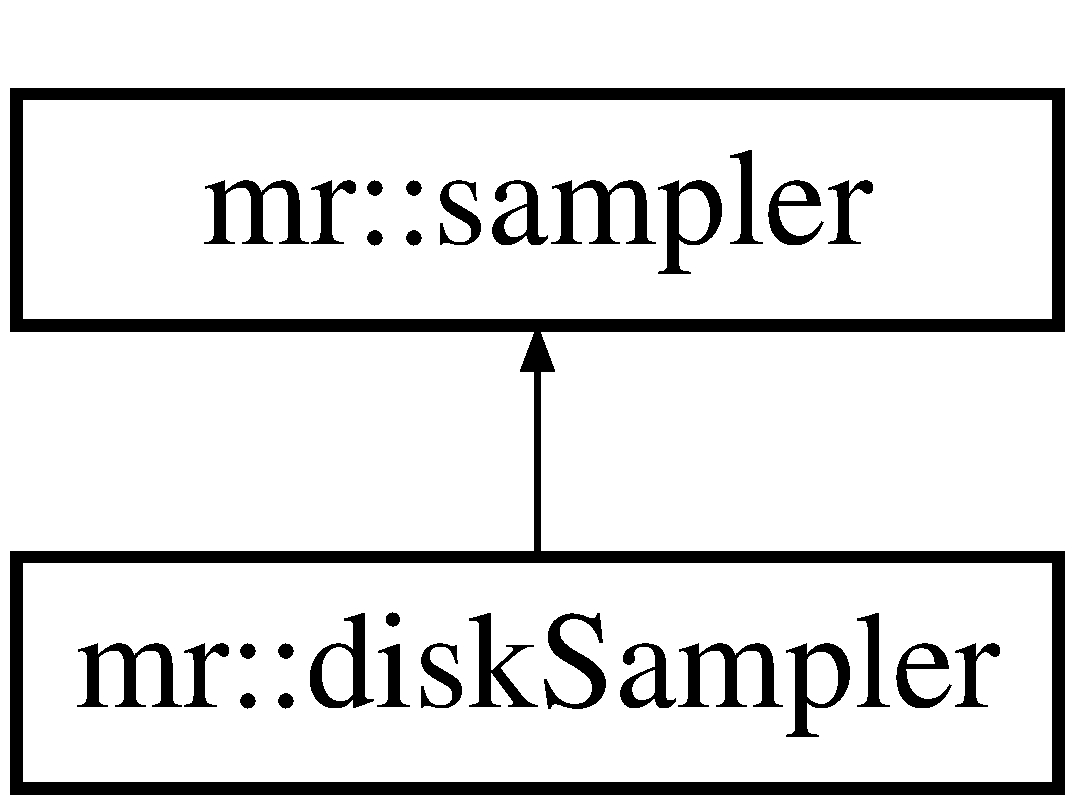
\includegraphics[height=2cm]{classmr_1_1diskSampler}
\end{center}
\end{figure}
\subsection*{Public Member Functions}
\begin{CompactItemize}
\item 
{\bf disk\-Sampler} ()
\item 
{\bf disk\-Sampler} (const mi\-Uint \&num\-Samples)
\item 
{\bf $\sim$disk\-Sampler} ()
\item 
bool {\bf uniform} (const mi\-State $\ast$const)
\begin{CompactList}\small\item\em Get one sample using a uniform distribution or return false. \item\end{CompactList}\item 
bool {\bf concentric} (const mi\-State $\ast$const)
\begin{CompactList}\small\item\em Get one sample using a concentric distribution or return false. \item\end{CompactList}\item 
const mi\-Vector2d \& {\bf position} ()
\begin{CompactList}\small\item\em Return u,v position of sample. \item\end{CompactList}\end{CompactItemize}
\subsection*{Protected Member Functions}
\begin{CompactItemize}
\item 
void {\bf concentric\-Distribution} ()
\item 
void {\bf uniform\-Distribution} ()
\end{CompactItemize}


\subsection{Detailed Description}
Sample in a disk. 



\subsection{Constructor \& Destructor Documentation}
\index{mr::diskSampler@{mr::disk\-Sampler}!diskSampler@{diskSampler}}
\index{diskSampler@{diskSampler}!mr::diskSampler@{mr::disk\-Sampler}}
\subsubsection{\setlength{\rightskip}{0pt plus 5cm}mr::disk\-Sampler::disk\-Sampler ()\hspace{0.3cm}{\tt  [inline]}}\label{classmr_1_1diskSampler_a0}


Constructor. This call is to be used when sampling adaptively (ie. the number of samples to be taken are not known or may vary, or you may exit the loop early). \index{mr::diskSampler@{mr::disk\-Sampler}!diskSampler@{diskSampler}}
\index{diskSampler@{diskSampler}!mr::diskSampler@{mr::disk\-Sampler}}
\subsubsection{\setlength{\rightskip}{0pt plus 5cm}mr::disk\-Sampler::disk\-Sampler (const mi\-Uint \& {\em num\-Samples})\hspace{0.3cm}{\tt  [inline]}}\label{classmr_1_1diskSampler_a1}


Constructor. Fixed Sampling. num\-Samples is the number of samples to take. It HAS to be mi\-Uint\& \index{mr::diskSampler@{mr::disk\-Sampler}!~diskSampler@{$\sim$diskSampler}}
\index{~diskSampler@{$\sim$diskSampler}!mr::diskSampler@{mr::disk\-Sampler}}
\subsubsection{\setlength{\rightskip}{0pt plus 5cm}mr::disk\-Sampler::$\sim${\bf disk\-Sampler} ()\hspace{0.3cm}{\tt  [inline]}}\label{classmr_1_1diskSampler_a2}




\subsection{Member Function Documentation}
\index{mr::diskSampler@{mr::disk\-Sampler}!concentric@{concentric}}
\index{concentric@{concentric}!mr::diskSampler@{mr::disk\-Sampler}}
\subsubsection{\setlength{\rightskip}{0pt plus 5cm}bool mr::disk\-Sampler::concentric (const mi\-State $\ast$ {\em const })\hspace{0.3cm}{\tt  [inline]}}\label{classmr_1_1diskSampler_a4}


Get one sample using a concentric distribution or return false. 

\index{mr::diskSampler@{mr::disk\-Sampler}!concentricDistribution@{concentricDistribution}}
\index{concentricDistribution@{concentricDistribution}!mr::diskSampler@{mr::disk\-Sampler}}
\subsubsection{\setlength{\rightskip}{0pt plus 5cm}void mr::disk\-Sampler::concentric\-Distribution ()\hspace{0.3cm}{\tt  [inline, protected]}}\label{classmr_1_1diskSampler_b0}


\index{mr::diskSampler@{mr::disk\-Sampler}!position@{position}}
\index{position@{position}!mr::diskSampler@{mr::disk\-Sampler}}
\subsubsection{\setlength{\rightskip}{0pt plus 5cm}const mi\-Vector2d\& mr::disk\-Sampler::position ()\hspace{0.3cm}{\tt  [inline]}}\label{classmr_1_1diskSampler_a5}


Return u,v position of sample. 

\index{mr::diskSampler@{mr::disk\-Sampler}!uniform@{uniform}}
\index{uniform@{uniform}!mr::diskSampler@{mr::disk\-Sampler}}
\subsubsection{\setlength{\rightskip}{0pt plus 5cm}bool mr::disk\-Sampler::uniform (const mi\-State $\ast$ {\em const })\hspace{0.3cm}{\tt  [inline]}}\label{classmr_1_1diskSampler_a3}


Get one sample using a uniform distribution or return false. 

\index{mr::diskSampler@{mr::disk\-Sampler}!uniformDistribution@{uniformDistribution}}
\index{uniformDistribution@{uniformDistribution}!mr::diskSampler@{mr::disk\-Sampler}}
\subsubsection{\setlength{\rightskip}{0pt plus 5cm}void mr::disk\-Sampler::uniform\-Distribution ()\hspace{0.3cm}{\tt  [inline, protected]}}\label{classmr_1_1diskSampler_b1}




The documentation for this class was generated from the following file:\begin{CompactItemize}
\item 
{\bf mr\-Sampler.h}\end{CompactItemize}

\section{mr::base::div Struct Reference}
\label{structmr_1_1base_1_1div}\index{mr::base::div@{mr::base::div}}
{\tt \#include $<$mr\-Base.h$>$}

\subsection*{Static Public Member Functions}
\begin{CompactItemize}
\item 
template$<$class ta\_\-a, class ta\_\-b$>$ const double {\bf Evaluate} (const unsigned short i, const ta\_\-a \&A, const ta\_\-b \&B)
\end{CompactItemize}


\subsection{Member Function Documentation}
\index{mr::base::div@{mr::base::div}!Evaluate@{Evaluate}}
\index{Evaluate@{Evaluate}!mr::base::div@{mr::base::div}}
\subsubsection{\setlength{\rightskip}{0pt plus 5cm}template$<$class ta\_\-a, class ta\_\-b$>$ const double mr::base::div::Evaluate (const unsigned short {\em i}, const ta\_\-a \& {\em A}, const ta\_\-b \& {\em B})\hspace{0.3cm}{\tt  [inline, static]}}\label{structmr_1_1base_1_1div_e0}




The documentation for this struct was generated from the following file:\begin{CompactItemize}
\item 
{\bf mr\-Base.h}\end{CompactItemize}

\section{mr::errorbuffer Struct Reference}
\label{structmr_1_1errorbuffer}\index{mr::errorbuffer@{mr::errorbuffer}}
{\tt \#include $<$mr\-Stream.h$>$}

Inheritance diagram for mr::errorbuffer::\begin{figure}[H]
\begin{center}
\leavevmode
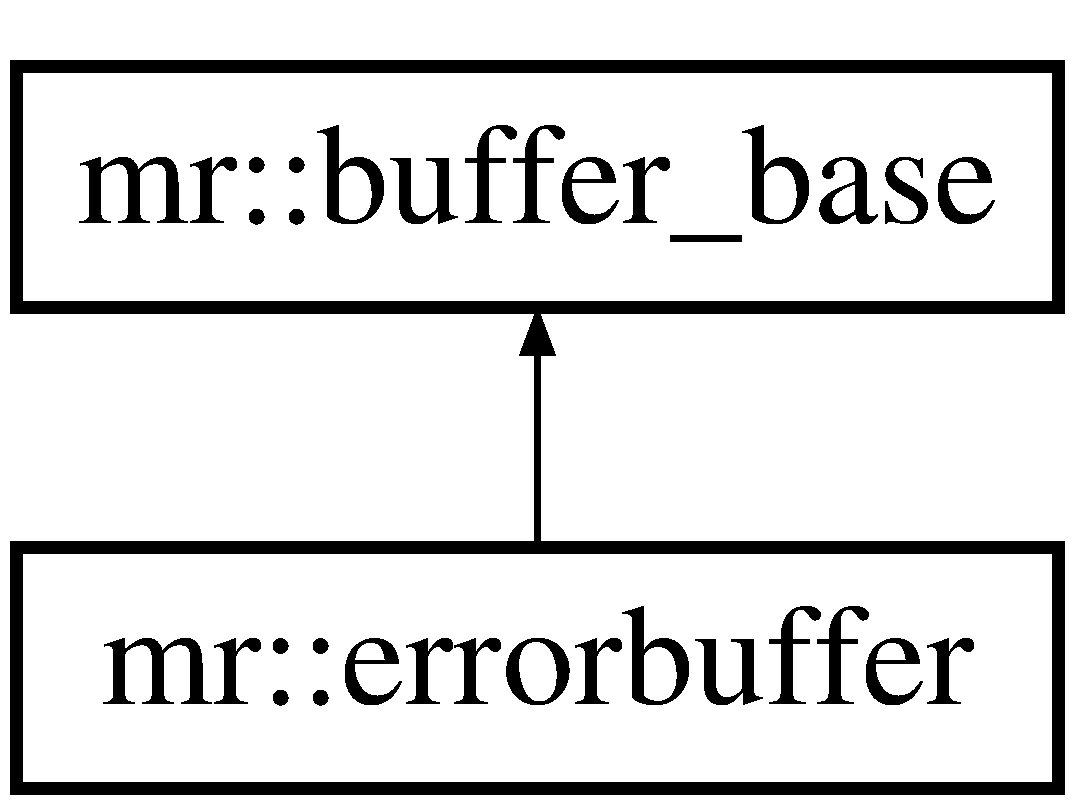
\includegraphics[height=2cm]{structmr_1_1errorbuffer}
\end{center}
\end{figure}
\subsection*{Public Member Functions}
\begin{CompactItemize}
\item 
{\bf errorbuffer} ()
\item 
virtual void {\bf print} (const char $\ast$const s)
\begin{CompactList}\small\item\em virtual function to print string out \item\end{CompactList}\end{CompactItemize}


\subsection{Constructor \& Destructor Documentation}
\index{mr::errorbuffer@{mr::errorbuffer}!errorbuffer@{errorbuffer}}
\index{errorbuffer@{errorbuffer}!mr::errorbuffer@{mr::errorbuffer}}
\subsubsection{\setlength{\rightskip}{0pt plus 5cm}mr::errorbuffer::errorbuffer ()\hspace{0.3cm}{\tt  [inline]}}\label{structmr_1_1errorbuffer_a0}




\subsection{Member Function Documentation}
\index{mr::errorbuffer@{mr::errorbuffer}!print@{print}}
\index{print@{print}!mr::errorbuffer@{mr::errorbuffer}}
\subsubsection{\setlength{\rightskip}{0pt plus 5cm}virtual void mr::errorbuffer::print (const char $\ast$const {\em s})\hspace{0.3cm}{\tt  [inline, virtual]}}\label{structmr_1_1errorbuffer_a1}


virtual function to print string out 



Implements {\bf mr::buffer\_\-base} {\rm (p.\,\pageref{structmr_1_1buffer__base_a3})}.

The documentation for this struct was generated from the following file:\begin{CompactItemize}
\item 
{\bf mr\-Stream.h}\end{CompactItemize}

\section{mr::errorstream Struct Reference}
\label{structmr_1_1errorstream}\index{mr::errorstream@{mr::errorstream}}
{\tt \#include $<$mr\-Stream.h$>$}

\subsection*{Public Member Functions}
\begin{CompactItemize}
\item 
{\bf errorstream} ()
\item 
{\bf $\sim$errorstream} ()
\end{CompactItemize}


\subsection{Constructor \& Destructor Documentation}
\index{mr::errorstream@{mr::errorstream}!errorstream@{errorstream}}
\index{errorstream@{errorstream}!mr::errorstream@{mr::errorstream}}
\subsubsection{\setlength{\rightskip}{0pt plus 5cm}mr::errorstream::errorstream ()\hspace{0.3cm}{\tt  [inline]}}\label{structmr_1_1errorstream_a0}


\index{mr::errorstream@{mr::errorstream}!~errorstream@{$\sim$errorstream}}
\index{~errorstream@{$\sim$errorstream}!mr::errorstream@{mr::errorstream}}
\subsubsection{\setlength{\rightskip}{0pt plus 5cm}mr::errorstream::$\sim${\bf errorstream} ()\hspace{0.3cm}{\tt  [inline]}}\label{structmr_1_1errorstream_a1}




The documentation for this struct was generated from the following file:\begin{CompactItemize}
\item 
{\bf mr\-Stream.h}\end{CompactItemize}

\section{mr::distances::Euclidian Struct Reference}
\label{structmr_1_1distances_1_1Euclidian}\index{mr::distances::Euclidian@{mr::distances::Euclidian}}
Functor to calculate euclidian distance ( squared ).  


{\tt \#include $<$mr\-Distances.h$>$}

Inheritance diagram for mr::distances::Euclidian::\begin{figure}[H]
\begin{center}
\leavevmode
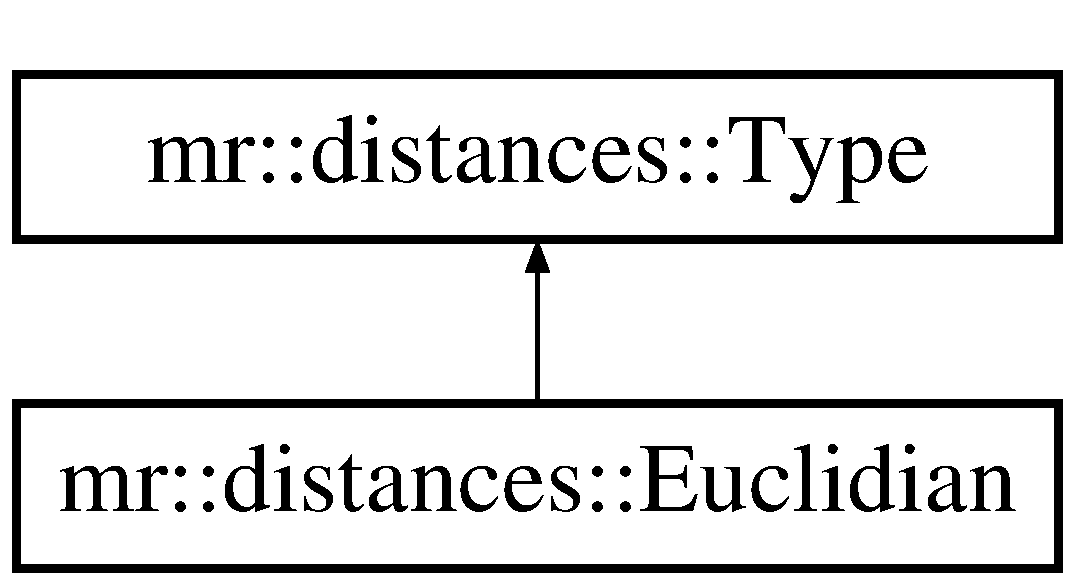
\includegraphics[height=2cm]{structmr_1_1distances_1_1Euclidian}
\end{center}
\end{figure}
\subsection*{Public Member Functions}
\begin{CompactItemize}
\item 
mi\-Scalar {\bf operator()} (const {\bf vector} \&d) const 
\item 
mi\-Scalar {\bf operator()} (const {\bf vector} \&d, const {\bf vector} \&s) const 
\end{CompactItemize}


\subsection{Detailed Description}
Functor to calculate euclidian distance ( squared ). 



\subsection{Member Function Documentation}
\index{mr::distances::Euclidian@{mr::distances::Euclidian}!operator()@{operator()}}
\index{operator()@{operator()}!mr::distances::Euclidian@{mr::distances::Euclidian}}
\subsubsection{\setlength{\rightskip}{0pt plus 5cm}mi\-Scalar mr::distances::Euclidian::operator() (const {\bf vector} \& {\em d}, const {\bf vector} \& {\em s}) const\hspace{0.3cm}{\tt  [inline, virtual]}}\label{structmr_1_1distances_1_1Euclidian_a1}




Implements {\bf mr::distances::Type} {\rm (p.\,\pageref{structmr_1_1distances_1_1Type_a1})}.\index{mr::distances::Euclidian@{mr::distances::Euclidian}!operator()@{operator()}}
\index{operator()@{operator()}!mr::distances::Euclidian@{mr::distances::Euclidian}}
\subsubsection{\setlength{\rightskip}{0pt plus 5cm}mi\-Scalar mr::distances::Euclidian::operator() (const {\bf vector} \& {\em d}) const\hspace{0.3cm}{\tt  [inline, virtual]}}\label{structmr_1_1distances_1_1Euclidian_a0}




Implements {\bf mr::distances::Type} {\rm (p.\,\pageref{structmr_1_1distances_1_1Type_a0})}.

The documentation for this struct was generated from the following file:\begin{CompactItemize}
\item 
{\bf mr\-Distances.h}\end{CompactItemize}

\section{Exception\-Handler Class Reference}
\label{classExceptionHandler}\index{ExceptionHandler@{ExceptionHandler}}
{\tt \#include $<$mr\-Stack\-Trace\_\-linux.h$>$}



The documentation for this class was generated from the following file:\begin{CompactItemize}
\item 
{\bf mr\-Stack\-Trace\_\-linux.h}\end{CompactItemize}

\section{mr::Exception\-Handler Class Reference}
\label{classmr_1_1ExceptionHandler}\index{mr::ExceptionHandler@{mr::ExceptionHandler}}
Exception handler.  


{\tt \#include $<$mr\-Stack\-Trace\_\-win32.h$>$}

\subsection*{Public Member Functions}
\begin{CompactItemize}
\item 
{\bf Exception\-Handler} ()
\begin{CompactList}\small\item\em Initialize Exception Handler. \item\end{CompactList}\item 
{\bf $\sim$Exception\-Handler} ()
\begin{CompactList}\small\item\em Destroy exception handler and restore original exceptions. \item\end{CompactList}\end{CompactItemize}
\subsection*{Static Public Member Functions}
\begin{CompactItemize}
\item 
void {\bf Show\-Stack} (HANDLE h\-Thread, CONTEXT \&c)
\begin{CompactList}\small\item\em Show a Stack Trace so far. \item\end{CompactList}\item 
void {\bf Set\-Log\-File\-Name} (PTSTR psz\-Log\-File\-Name)
\end{CompactItemize}


\subsection{Detailed Description}
Exception handler. 



\subsection{Constructor \& Destructor Documentation}
\index{mr::ExceptionHandler@{mr::Exception\-Handler}!ExceptionHandler@{ExceptionHandler}}
\index{ExceptionHandler@{ExceptionHandler}!mr::ExceptionHandler@{mr::Exception\-Handler}}
\subsubsection{\setlength{\rightskip}{0pt plus 5cm}mr::Exception\-Handler::Exception\-Handler ()}\label{classmr_1_1ExceptionHandler_a0}


Initialize Exception Handler. 

\index{mr::ExceptionHandler@{mr::Exception\-Handler}!~ExceptionHandler@{$\sim$ExceptionHandler}}
\index{~ExceptionHandler@{$\sim$ExceptionHandler}!mr::ExceptionHandler@{mr::Exception\-Handler}}
\subsubsection{\setlength{\rightskip}{0pt plus 5cm}mr::Exception\-Handler::$\sim${\bf Exception\-Handler} ()}\label{classmr_1_1ExceptionHandler_a1}


Destroy exception handler and restore original exceptions. 



\subsection{Member Function Documentation}
\index{mr::ExceptionHandler@{mr::Exception\-Handler}!SetLogFileName@{SetLogFileName}}
\index{SetLogFileName@{SetLogFileName}!mr::ExceptionHandler@{mr::Exception\-Handler}}
\subsubsection{\setlength{\rightskip}{0pt plus 5cm}void mr::Exception\-Handler::Set\-Log\-File\-Name (PTSTR {\em psz\-Log\-File\-Name})\hspace{0.3cm}{\tt  [static]}}\label{classmr_1_1ExceptionHandler_e1}


Set log file to dump trace and info in case of crash. Default name is name of the main program. \index{mr::ExceptionHandler@{mr::Exception\-Handler}!ShowStack@{ShowStack}}
\index{ShowStack@{ShowStack}!mr::ExceptionHandler@{mr::Exception\-Handler}}
\subsubsection{\setlength{\rightskip}{0pt plus 5cm}void mr::Exception\-Handler::Show\-Stack (HANDLE {\em h\-Thread}, CONTEXT \& {\em c})\hspace{0.3cm}{\tt  [static]}}\label{classmr_1_1ExceptionHandler_e0}


Show a Stack Trace so far. 



The documentation for this class was generated from the following file:\begin{CompactItemize}
\item 
{\bf mr\-Stack\-Trace\_\-win32.h}\end{CompactItemize}

\section{mr::base::exp$<$ ta\_\-a, ta\_\-b, ta\_\-eval $>$ Class Template Reference}
\label{classmr_1_1base_1_1exp}\index{mr::base::exp@{mr::base::exp}}
{\tt \#include $<$mr\-Base.h$>$}

\subsection*{Public Member Functions}
\begin{CompactItemize}
\item 
{\bf exp} (const ta\_\-a \&A1, const ta\_\-b \&A2)
\item 
const double {\bf Evaluate} (const unsigned short i) const 
\end{CompactItemize}
\subsubsection*{template$<$class ta\_\-a, class ta\_\-b, class ta\_\-eval$>$ class mr::base::exp$<$ ta\_\-a, ta\_\-b, ta\_\-eval $>$}



\subsection{Constructor \& Destructor Documentation}
\index{mr::base::exp@{mr::base::exp}!exp@{exp}}
\index{exp@{exp}!mr::base::exp@{mr::base::exp}}
\subsubsection{\setlength{\rightskip}{0pt plus 5cm}template$<$class ta\_\-a, class ta\_\-b, class ta\_\-eval$>$ {\bf mr::base::exp}$<$ ta\_\-a, ta\_\-b, ta\_\-eval $>$::{\bf exp} (const ta\_\-a \& {\em A1}, const ta\_\-b \& {\em A2})\hspace{0.3cm}{\tt  [inline]}}\label{classmr_1_1base_1_1exp_a0}




\subsection{Member Function Documentation}
\index{mr::base::exp@{mr::base::exp}!Evaluate@{Evaluate}}
\index{Evaluate@{Evaluate}!mr::base::exp@{mr::base::exp}}
\subsubsection{\setlength{\rightskip}{0pt plus 5cm}template$<$class ta\_\-a, class ta\_\-b, class ta\_\-eval$>$ const double {\bf mr::base::exp}$<$ ta\_\-a, ta\_\-b, ta\_\-eval $>$::Evaluate (const unsigned short {\em i}) const\hspace{0.3cm}{\tt  [inline]}}\label{classmr_1_1base_1_1exp_a1}




The documentation for this class was generated from the following file:\begin{CompactItemize}
\item 
{\bf mr\-Base.h}\end{CompactItemize}

\section{mr::fastmath$<$ T $>$ Class Template Reference}
\label{classmr_1_1fastmath}\index{mr::fastmath@{mr::fastmath}}
Encapsulates fast math tables / functions.  


{\tt \#include $<$mr\-Fast\-Math.h$>$}

\subsection*{Static Public Member Functions}
\begin{CompactItemize}
\item 
T {\bf sin0} (const T x)
\item 
T {\bf sin1} (const T x)
\item 
T {\bf cos0} (const T x)
\item 
T {\bf cos1} (const T x)
\item 
T {\bf tan0} (const T x)
\item 
T {\bf tan1} (const T x)
\item 
T {\bf asin} (const T x)
\item 
T {\bf acos} (const T x)
\item 
T {\bf atan0} (const T x)
\item 
T {\bf atan1} (const T x)
\item 
T {\bf invsqrt} (T x)
\begin{CompactList}\small\item\em A fast approximation to 1/sqrt. \item\end{CompactList}\item 
int {\bf floor} (T x)
\begin{CompactList}\small\item\em A fast and quite accurate approximation to floor(x) or int(float). \item\end{CompactList}\item 
int {\bf ceil} (T x)
\begin{CompactList}\small\item\em A fast and quite accurate approximation to ceil(x). \item\end{CompactList}\end{CompactItemize}


\subsection{Detailed Description}
\subsubsection*{template$<$class T$>$ class mr::fastmath$<$ T $>$}

Encapsulates fast math tables / functions. 



\subsection{Member Function Documentation}
\index{mr::fastmath@{mr::fastmath}!acos@{acos}}
\index{acos@{acos}!mr::fastmath@{mr::fastmath}}
\subsubsection{\setlength{\rightskip}{0pt plus 5cm}template$<$class T$>$ T {\bf mr::fastmath}$<$ T $>$::acos (const T {\em x})\hspace{0.3cm}{\tt  [inline, static]}}\label{classmr_1_1fastmath_e7}


Fast evaluation of acos(value) by a sqrt times a polynomial. The value must be in [0,1]. The maximum absolute error is about 6.8e-05 and the speed up is about 2.5. \index{mr::fastmath@{mr::fastmath}!asin@{asin}}
\index{asin@{asin}!mr::fastmath@{mr::fastmath}}
\subsubsection{\setlength{\rightskip}{0pt plus 5cm}template$<$class T$>$ T {\bf mr::fastmath}$<$ T $>$::asin (const T {\em x})\hspace{0.3cm}{\tt  [inline, static]}}\label{classmr_1_1fastmath_e6}


Fast evaluation of asin(value) by a sqrt times a polynomial. The value must be in [0,1]. The maximum absolute error is about 6.8e-05 and the speed up is about 2.5. \index{mr::fastmath@{mr::fastmath}!atan0@{atan0}}
\index{atan0@{atan0}!mr::fastmath@{mr::fastmath}}
\subsubsection{\setlength{\rightskip}{0pt plus 5cm}template$<$class T$>$ T {\bf mr::fastmath}$<$ T $>$::atan0 (const T {\em x})\hspace{0.3cm}{\tt  [inline, static]}}\label{classmr_1_1fastmath_e8}


Fast evaluation of atan(value) by polynomial approximations. The value must be in [-1,1]. The maximum absolute error is about 1.2e-05 when templated as doubles. The speed up is about 2.2. \index{mr::fastmath@{mr::fastmath}!atan1@{atan1}}
\index{atan1@{atan1}!mr::fastmath@{mr::fastmath}}
\subsubsection{\setlength{\rightskip}{0pt plus 5cm}template$<$class T$>$ T {\bf mr::fastmath}$<$ T $>$::atan1 (const T {\em x})\hspace{0.3cm}{\tt  [inline, static]}}\label{classmr_1_1fastmath_e9}


Fast evaluation of atan(value) by polynomial approximations. The value must be in [-1,1]. The maximum absolute error is about 1.43-08 when templated as doubles. The speed up is about 1.5. \index{mr::fastmath@{mr::fastmath}!ceil@{ceil}}
\index{ceil@{ceil}!mr::fastmath@{mr::fastmath}}
\subsubsection{\setlength{\rightskip}{0pt plus 5cm}template$<$class T$>$ int {\bf mr::fastmath}$<$ T $>$::ceil (T {\em x})\hspace{0.3cm}{\tt  [inline, static]}}\label{classmr_1_1fastmath_e12}


A fast and quite accurate approximation to ceil(x). 

\index{mr::fastmath@{mr::fastmath}!cos0@{cos0}}
\index{cos0@{cos0}!mr::fastmath@{mr::fastmath}}
\subsubsection{\setlength{\rightskip}{0pt plus 5cm}template$<$class T$>$ T {\bf mr::fastmath}$<$ T $>$::cos0 (const T {\em x})\hspace{0.3cm}{\tt  [inline, static]}}\label{classmr_1_1fastmath_e2}


Fast evaluation of cos(angle) by polynomial approximations. The angle must be in [0,pi/2]. The maximum absolute error is about 1.2e-03 and the speed up is about 2 when templated as doubles. \index{mr::fastmath@{mr::fastmath}!cos1@{cos1}}
\index{cos1@{cos1}!mr::fastmath@{mr::fastmath}}
\subsubsection{\setlength{\rightskip}{0pt plus 5cm}template$<$class T$>$ T {\bf mr::fastmath}$<$ T $>$::cos1 (const T {\em x})\hspace{0.3cm}{\tt  [inline, static]}}\label{classmr_1_1fastmath_e3}


Fast evaluation of cos(angle) by polynomial approximations. The angle must be in [0,pi/2]. The maximum absolute error is about 2.3e-09 and the speed up is about 1.5 when templated as doubles. \index{mr::fastmath@{mr::fastmath}!floor@{floor}}
\index{floor@{floor}!mr::fastmath@{mr::fastmath}}
\subsubsection{\setlength{\rightskip}{0pt plus 5cm}template$<$class T$>$ int {\bf mr::fastmath}$<$ T $>$::floor (T {\em x})\hspace{0.3cm}{\tt  [inline, static]}}\label{classmr_1_1fastmath_e11}


A fast and quite accurate approximation to floor(x) or int(float). 

\index{mr::fastmath@{mr::fastmath}!invsqrt@{invsqrt}}
\index{invsqrt@{invsqrt}!mr::fastmath@{mr::fastmath}}
\subsubsection{\setlength{\rightskip}{0pt plus 5cm}template$<$class T$>$ T {\bf mr::fastmath}$<$ T $>$::invsqrt (T {\em x})\hspace{0.3cm}{\tt  [inline, static]}}\label{classmr_1_1fastmath_e10}


A fast approximation to 1/sqrt. 

This {\bf invsqrt()}{\rm (p.\,\pageref{classmr_1_1fastmath_e10})} is attributed to Quake. It was published in comp.graphics.algorithms and now David Eberly keeps a copy in his Magic-Software web site.

Comparing it to the Apple {\bf invsqrt()}{\rm (p.\,\pageref{classmr_1_1fastmath_e10})} and those from Gems, I found this one to be a tad faster, and use no memory. Input; x $>$ 0. Else routine does not work. This routine should be 10 to 20 times faster than using 1.0/sqrt(x). See Dave Eberly's notes at www.magic-software.com \index{mr::fastmath@{mr::fastmath}!sin0@{sin0}}
\index{sin0@{sin0}!mr::fastmath@{mr::fastmath}}
\subsubsection{\setlength{\rightskip}{0pt plus 5cm}template$<$class T$>$ T {\bf mr::fastmath}$<$ T $>$::sin0 (const T {\em x})\hspace{0.3cm}{\tt  [inline, static]}}\label{classmr_1_1fastmath_e0}


Fast evaluation of sin(angle) by polynomial approximations. The angle must be in [0,pi/2]. The maximum absolute error is about 1.7e-04 and speed up is about 2 when templated as doubles. \index{mr::fastmath@{mr::fastmath}!sin1@{sin1}}
\index{sin1@{sin1}!mr::fastmath@{mr::fastmath}}
\subsubsection{\setlength{\rightskip}{0pt plus 5cm}template$<$class T$>$ T {\bf mr::fastmath}$<$ T $>$::sin1 (const T {\em x})\hspace{0.3cm}{\tt  [inline, static]}}\label{classmr_1_1fastmath_e1}


Fast evaluation of sin(angle) by polynomial approximations. The angle must be in [0,pi/2]. The maximum absolute error is about 2.3e-09 and speed up is about 1.5 when templated as doubles. \index{mr::fastmath@{mr::fastmath}!tan0@{tan0}}
\index{tan0@{tan0}!mr::fastmath@{mr::fastmath}}
\subsubsection{\setlength{\rightskip}{0pt plus 5cm}template$<$class T$>$ T {\bf mr::fastmath}$<$ T $>$::tan0 (const T {\em x})\hspace{0.3cm}{\tt  [inline, static]}}\label{classmr_1_1fastmath_e4}


Fast evaluation of tan(angle) by polynomial approximations. The angle must be in [0,pi/4]. The maximum absolute error is about 8.1e-04 for when templated as doubles. The speed up is about 2.5. \index{mr::fastmath@{mr::fastmath}!tan1@{tan1}}
\index{tan1@{tan1}!mr::fastmath@{mr::fastmath}}
\subsubsection{\setlength{\rightskip}{0pt plus 5cm}template$<$class T$>$ T {\bf mr::fastmath}$<$ T $>$::tan1 (const T {\em x})\hspace{0.3cm}{\tt  [inline, static]}}\label{classmr_1_1fastmath_e5}


Fast evaluation of tan(angle) by polynomial approximations. The angle must be in [0,pi/4]. The maximum absolute error is about 1.9e-08 for tan1 when templated as doubles and The speed up is about 1.75. 

The documentation for this class was generated from the following file:\begin{CompactItemize}
\item 
{\bf mr\-Fast\-Math.h}\end{CompactItemize}

\section{mr::fatalbuffer Struct Reference}
\label{structmr_1_1fatalbuffer}\index{mr::fatalbuffer@{mr::fatalbuffer}}
{\tt \#include $<$mr\-Stream.h$>$}

Inheritance diagram for mr::fatalbuffer::\begin{figure}[H]
\begin{center}
\leavevmode
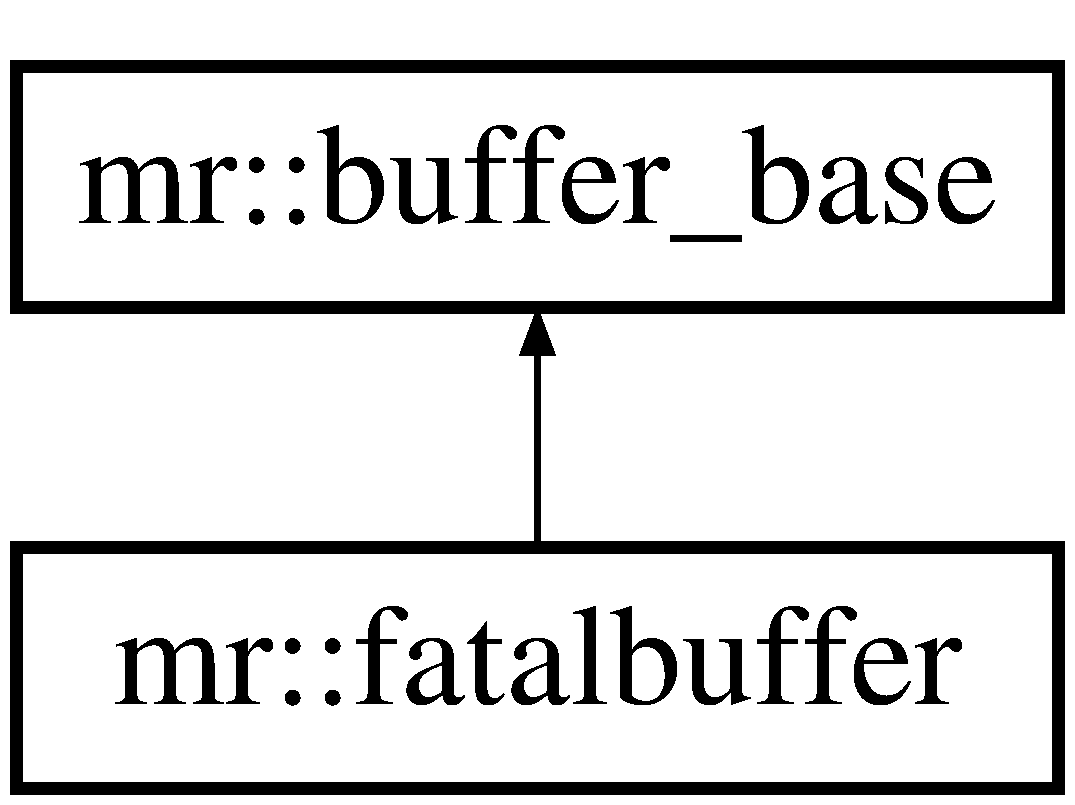
\includegraphics[height=2cm]{structmr_1_1fatalbuffer}
\end{center}
\end{figure}
\subsection*{Public Member Functions}
\begin{CompactItemize}
\item 
{\bf fatalbuffer} ()
\item 
virtual void {\bf print} (const char $\ast$const s)
\begin{CompactList}\small\item\em virtual function to print string out \item\end{CompactList}\end{CompactItemize}


\subsection{Constructor \& Destructor Documentation}
\index{mr::fatalbuffer@{mr::fatalbuffer}!fatalbuffer@{fatalbuffer}}
\index{fatalbuffer@{fatalbuffer}!mr::fatalbuffer@{mr::fatalbuffer}}
\subsubsection{\setlength{\rightskip}{0pt plus 5cm}mr::fatalbuffer::fatalbuffer ()\hspace{0.3cm}{\tt  [inline]}}\label{structmr_1_1fatalbuffer_a0}




\subsection{Member Function Documentation}
\index{mr::fatalbuffer@{mr::fatalbuffer}!print@{print}}
\index{print@{print}!mr::fatalbuffer@{mr::fatalbuffer}}
\subsubsection{\setlength{\rightskip}{0pt plus 5cm}virtual void mr::fatalbuffer::print (const char $\ast$const {\em s})\hspace{0.3cm}{\tt  [inline, virtual]}}\label{structmr_1_1fatalbuffer_a1}


virtual function to print string out 



Implements {\bf mr::buffer\_\-base} {\rm (p.\,\pageref{structmr_1_1buffer__base_a3})}.

The documentation for this struct was generated from the following file:\begin{CompactItemize}
\item 
{\bf mr\-Stream.h}\end{CompactItemize}

\section{mr::fatalstream Struct Reference}
\label{structmr_1_1fatalstream}\index{mr::fatalstream@{mr::fatalstream}}
{\tt \#include $<$mr\-Stream.h$>$}

\subsection*{Public Member Functions}
\begin{CompactItemize}
\item 
{\bf fatalstream} ()
\item 
{\bf $\sim$fatalstream} ()
\end{CompactItemize}


\subsection{Constructor \& Destructor Documentation}
\index{mr::fatalstream@{mr::fatalstream}!fatalstream@{fatalstream}}
\index{fatalstream@{fatalstream}!mr::fatalstream@{mr::fatalstream}}
\subsubsection{\setlength{\rightskip}{0pt plus 5cm}mr::fatalstream::fatalstream ()\hspace{0.3cm}{\tt  [inline]}}\label{structmr_1_1fatalstream_a0}


\index{mr::fatalstream@{mr::fatalstream}!~fatalstream@{$\sim$fatalstream}}
\index{~fatalstream@{$\sim$fatalstream}!mr::fatalstream@{mr::fatalstream}}
\subsubsection{\setlength{\rightskip}{0pt plus 5cm}mr::fatalstream::$\sim${\bf fatalstream} ()\hspace{0.3cm}{\tt  [inline]}}\label{structmr_1_1fatalstream_a1}




The documentation for this struct was generated from the following file:\begin{CompactItemize}
\item 
{\bf mr\-Stream.h}\end{CompactItemize}

\section{mr::FCell Class Reference}
\label{classmr_1_1FCell}\index{mr::FCell@{mr::FCell}}
Cellnoise class returning a float.  


{\tt \#include $<$mr\-Cell.h$>$}

\subsection*{Static Public Member Functions}
\begin{CompactItemize}
\item 
mi\-Scalar {\bf noise} (mi\-Scalar x)
\item 
mi\-Scalar {\bf noise} (mi\-Scalar x, mi\-Scalar y)
\item 
mi\-Scalar {\bf noise} (mi\-Scalar x, mi\-Scalar y, mi\-Scalar z)
\item 
mi\-Scalar {\bf noise} (mi\-Scalar x, mi\-Scalar y, mi\-Scalar z, mi\-Scalar t)
\item 
mi\-Scalar {\bf noise} (const {\bf vector2d} \&{\bf P})
\item 
mi\-Scalar {\bf noise} (const {\bf point} \&{\bf P})
\item 
mi\-Scalar {\bf noise} (const {\bf point} \&{\bf P}, const mi\-Scalar t)
\end{CompactItemize}
\subsection*{Public Attributes}
\begin{CompactItemize}
\item 
friend {\bf VCell}
\end{CompactItemize}
\subsection*{Static Protected Attributes}
\begin{CompactItemize}
\item 
const int {\bf TABLE\_\-SIZE} = 2048
\item 
const int {\bf MASK} = {\bf TABLE\_\-SIZE} - 1
\item 
MR\_\-LIB\_\-EXPORT int {\bf P} [$\,$]
\item 
MR\_\-LIB\_\-EXPORT float {\bf R} [$\,$]
\end{CompactItemize}


\subsection{Detailed Description}
Cellnoise class returning a float. 



\subsection{Member Function Documentation}
\index{mr::FCell@{mr::FCell}!noise@{noise}}
\index{noise@{noise}!mr::FCell@{mr::FCell}}
\subsubsection{\setlength{\rightskip}{0pt plus 5cm}mi\-Scalar mr::FCell::noise (const {\bf point} \& {\em P}, const mi\-Scalar {\em t})\hspace{0.3cm}{\tt  [inline, static]}}\label{classmr_1_1FCell_e6}


\index{mr::FCell@{mr::FCell}!noise@{noise}}
\index{noise@{noise}!mr::FCell@{mr::FCell}}
\subsubsection{\setlength{\rightskip}{0pt plus 5cm}mi\-Scalar mr::FCell::noise (const {\bf point} \& {\em P})\hspace{0.3cm}{\tt  [inline, static]}}\label{classmr_1_1FCell_e5}


\index{mr::FCell@{mr::FCell}!noise@{noise}}
\index{noise@{noise}!mr::FCell@{mr::FCell}}
\subsubsection{\setlength{\rightskip}{0pt plus 5cm}mi\-Scalar mr::FCell::noise (const {\bf vector2d} \& {\em P})\hspace{0.3cm}{\tt  [inline, static]}}\label{classmr_1_1FCell_e4}


\index{mr::FCell@{mr::FCell}!noise@{noise}}
\index{noise@{noise}!mr::FCell@{mr::FCell}}
\subsubsection{\setlength{\rightskip}{0pt plus 5cm}mi\-Scalar mr::FCell::noise (mi\-Scalar {\em x}, mi\-Scalar {\em y}, mi\-Scalar {\em z}, mi\-Scalar {\em t})\hspace{0.3cm}{\tt  [inline, static]}}\label{classmr_1_1FCell_e3}


\index{mr::FCell@{mr::FCell}!noise@{noise}}
\index{noise@{noise}!mr::FCell@{mr::FCell}}
\subsubsection{\setlength{\rightskip}{0pt plus 5cm}mi\-Scalar mr::FCell::noise (mi\-Scalar {\em x}, mi\-Scalar {\em y}, mi\-Scalar {\em z})\hspace{0.3cm}{\tt  [inline, static]}}\label{classmr_1_1FCell_e2}


\index{mr::FCell@{mr::FCell}!noise@{noise}}
\index{noise@{noise}!mr::FCell@{mr::FCell}}
\subsubsection{\setlength{\rightskip}{0pt plus 5cm}mi\-Scalar mr::FCell::noise (mi\-Scalar {\em x}, mi\-Scalar {\em y})\hspace{0.3cm}{\tt  [inline, static]}}\label{classmr_1_1FCell_e1}


\index{mr::FCell@{mr::FCell}!noise@{noise}}
\index{noise@{noise}!mr::FCell@{mr::FCell}}
\subsubsection{\setlength{\rightskip}{0pt plus 5cm}mi\-Scalar mr::FCell::noise (mi\-Scalar {\em x})\hspace{0.3cm}{\tt  [inline, static]}}\label{classmr_1_1FCell_e0}




\subsection{Member Data Documentation}
\index{mr::FCell@{mr::FCell}!MASK@{MASK}}
\index{MASK@{MASK}!mr::FCell@{mr::FCell}}
\subsubsection{\setlength{\rightskip}{0pt plus 5cm}const int {\bf mr::FCell::MASK} = {\bf TABLE\_\-SIZE} - 1\hspace{0.3cm}{\tt  [static, protected]}}\label{classmr_1_1FCell_t1}


\index{mr::FCell@{mr::FCell}!P@{P}}
\index{P@{P}!mr::FCell@{mr::FCell}}
\subsubsection{\setlength{\rightskip}{0pt plus 5cm}MR\_\-LIB\_\-EXPORT int {\bf mr::FCell::P}[$\,$]\hspace{0.3cm}{\tt  [static, protected]}}\label{classmr_1_1FCell_t2}


\index{mr::FCell@{mr::FCell}!R@{R}}
\index{R@{R}!mr::FCell@{mr::FCell}}
\subsubsection{\setlength{\rightskip}{0pt plus 5cm}MR\_\-LIB\_\-EXPORT float {\bf mr::FCell::R}[$\,$]\hspace{0.3cm}{\tt  [static, protected]}}\label{classmr_1_1FCell_t3}


\index{mr::FCell@{mr::FCell}!TABLE_SIZE@{TABLE\_\-SIZE}}
\index{TABLE_SIZE@{TABLE\_\-SIZE}!mr::FCell@{mr::FCell}}
\subsubsection{\setlength{\rightskip}{0pt plus 5cm}const int {\bf mr::FCell::TABLE\_\-SIZE} = 2048\hspace{0.3cm}{\tt  [static, protected]}}\label{classmr_1_1FCell_t0}


\index{mr::FCell@{mr::FCell}!VCell@{VCell}}
\index{VCell@{VCell}!mr::FCell@{mr::FCell}}
\subsubsection{\setlength{\rightskip}{0pt plus 5cm}friend {\bf mr::FCell::VCell}}\label{classmr_1_1FCell_o0}




The documentation for this class was generated from the following file:\begin{CompactItemize}
\item 
{\bf mr\-Cell.h}\end{CompactItemize}

\section{mr::FWorley Class Reference}
\label{classmr_1_1FWorley}\index{mr::FWorley@{mr::FWorley}}
Worley noise class returning arbitrary number of floats.  


{\tt \#include $<$mr\-Worley.h$>$}

\subsection*{Static Public Member Functions}
\begin{CompactItemize}
\item 
MR\_\-LIB\_\-EXPORT void {\bf noise} (const mi\-Scalar x, const mi\-Scalar y, const mi\-Scalar z, const mi\-Ulong max\_\-order, mi\-Scalar $\ast$const F, mi\-Vector $\ast$const delta=NULL, mi\-Ulong $\ast$const ID=NULL)
\item 
void {\bf noise} (const mi\-Vector \&P, const mi\-Ulong max\_\-order, mi\-Scalar $\ast$const F, mi\-Vector $\ast$const delta=NULL, mi\-Ulong $\ast$const ID=NULL)
\item 
MR\_\-LIB\_\-EXPORT void {\bf noise} (const {\bf mr::distances::Type} \&Distance\-Measure, const mi\-Vector \&scale, const mi\-Scalar x, const mi\-Scalar y, const mi\-Scalar z, const mi\-Ulong max\_\-order, mi\-Scalar $\ast$const F, mi\-Vector $\ast$const delta=NULL, mi\-Ulong $\ast$const ID=NULL)
\item 
void {\bf noise} (const {\bf mr::distances::Type} \&Distance\-Measure, const mi\-Vector \&scale, const mi\-Vector \&P, const mi\-Ulong max\_\-order, mi\-Scalar $\ast$const F, mi\-Vector $\ast$const delta=NULL, mi\-Ulong $\ast$const ID=NULL)
\end{CompactItemize}
\subsection*{Static Protected Member Functions}
\begin{CompactItemize}
\item 
void {\bf Add\-Samples} (const long xi, const long yi, const long zi, const mi\-Ulong max\_\-order, const mi\-Vector \&at, mi\-Scalar $\ast$const F, mi\-Vector $\ast$const delta, mi\-Ulong $\ast$const ID)
\item 
void {\bf Add\-Samples} (const {\bf mr::distances::Type} \&Distance\-Measure, const mi\-Vector \&scale, const long xi, const long yi, const long zi, const mi\-Ulong max\_\-order, const mi\-Vector \&at, mi\-Scalar $\ast$const F, mi\-Vector $\ast$const delta, mi\-Ulong $\ast$const ID)
\end{CompactItemize}


\subsection{Detailed Description}
Worley noise class returning arbitrary number of floats. 



\subsection{Member Function Documentation}
\index{mr::FWorley@{mr::FWorley}!AddSamples@{AddSamples}}
\index{AddSamples@{AddSamples}!mr::FWorley@{mr::FWorley}}
\subsubsection{\setlength{\rightskip}{0pt plus 5cm}void mr::FWorley::Add\-Samples (const {\bf mr::distances::Type} \& {\em Distance\-Measure}, const mi\-Vector \& {\em scale}, const long {\em xi}, const long {\em yi}, const long {\em zi}, const mi\-Ulong {\em max\_\-order}, const mi\-Vector \& {\em at}, mi\-Scalar $\ast$const {\em F}, mi\-Vector $\ast$const {\em delta}, mi\-Ulong $\ast$const {\em ID})\hspace{0.3cm}{\tt  [static, protected]}}\label{classmr_1_1FWorley_f1}


\index{mr::FWorley@{mr::FWorley}!AddSamples@{AddSamples}}
\index{AddSamples@{AddSamples}!mr::FWorley@{mr::FWorley}}
\subsubsection{\setlength{\rightskip}{0pt plus 5cm}void mr::FWorley::Add\-Samples (const long {\em xi}, const long {\em yi}, const long {\em zi}, const mi\-Ulong {\em max\_\-order}, const mi\-Vector \& {\em at}, mi\-Scalar $\ast$const {\em F}, mi\-Vector $\ast$const {\em delta}, mi\-Ulong $\ast$const {\em ID})\hspace{0.3cm}{\tt  [static, protected]}}\label{classmr_1_1FWorley_f0}


the function to merge-sort a \char`\"{}cube\char`\"{} of samples into the current best-found list of values. \index{mr::FWorley@{mr::FWorley}!noise@{noise}}
\index{noise@{noise}!mr::FWorley@{mr::FWorley}}
\subsubsection{\setlength{\rightskip}{0pt plus 5cm}void mr::FWorley::noise (const {\bf mr::distances::Type} \& {\em Distance\-Measure}, const mi\-Vector \& {\em scale}, const mi\-Vector \& {\em P}, const mi\-Ulong {\em max\_\-order}, mi\-Scalar $\ast$const {\em F}, mi\-Vector $\ast$const {\em delta} = NULL, mi\-Ulong $\ast$const {\em ID} = NULL)\hspace{0.3cm}{\tt  [inline, static]}}\label{classmr_1_1FWorley_e3}


\index{mr::FWorley@{mr::FWorley}!noise@{noise}}
\index{noise@{noise}!mr::FWorley@{mr::FWorley}}
\subsubsection{\setlength{\rightskip}{0pt plus 5cm}MR\_\-LIB\_\-EXPORT void mr::FWorley::noise (const {\bf mr::distances::Type} \& {\em Distance\-Measure}, const mi\-Vector \& {\em scale}, const mi\-Scalar {\em x}, const mi\-Scalar {\em y}, const mi\-Scalar {\em z}, const mi\-Ulong {\em max\_\-order}, mi\-Scalar $\ast$const {\em F}, mi\-Vector $\ast$const {\em delta} = NULL, mi\-Ulong $\ast$const {\em ID} = NULL)\hspace{0.3cm}{\tt  [static]}}\label{classmr_1_1FWorley_e2}


\index{mr::FWorley@{mr::FWorley}!noise@{noise}}
\index{noise@{noise}!mr::FWorley@{mr::FWorley}}
\subsubsection{\setlength{\rightskip}{0pt plus 5cm}void mr::FWorley::noise (const mi\-Vector \& {\em P}, const mi\-Ulong {\em max\_\-order}, mi\-Scalar $\ast$const {\em F}, mi\-Vector $\ast$const {\em delta} = NULL, mi\-Ulong $\ast$const {\em ID} = NULL)\hspace{0.3cm}{\tt  [inline, static]}}\label{classmr_1_1FWorley_e1}


\index{mr::FWorley@{mr::FWorley}!noise@{noise}}
\index{noise@{noise}!mr::FWorley@{mr::FWorley}}
\subsubsection{\setlength{\rightskip}{0pt plus 5cm}MR\_\-LIB\_\-EXPORT void mr::FWorley::noise (const mi\-Scalar {\em x}, const mi\-Scalar {\em y}, const mi\-Scalar {\em z}, const mi\-Ulong {\em max\_\-order}, mi\-Scalar $\ast$const {\em F}, mi\-Vector $\ast$const {\em delta} = NULL, mi\-Ulong $\ast$const {\em ID} = NULL)\hspace{0.3cm}{\tt  [static]}}\label{classmr_1_1FWorley_e0}




The documentation for this class was generated from the following file:\begin{CompactItemize}
\item 
{\bf mr\-Worley.h}\end{CompactItemize}

\section{mr::hemisphere\-Sampler Class Reference}
\label{classmr_1_1hemisphereSampler}\index{mr::hemisphereSampler@{mr::hemisphereSampler}}
Sample a full or partial hemisphere around a direction.  


{\tt \#include $<$mr\-Sampler.h$>$}

Inheritance diagram for mr::hemisphere\-Sampler::\begin{figure}[H]
\begin{center}
\leavevmode
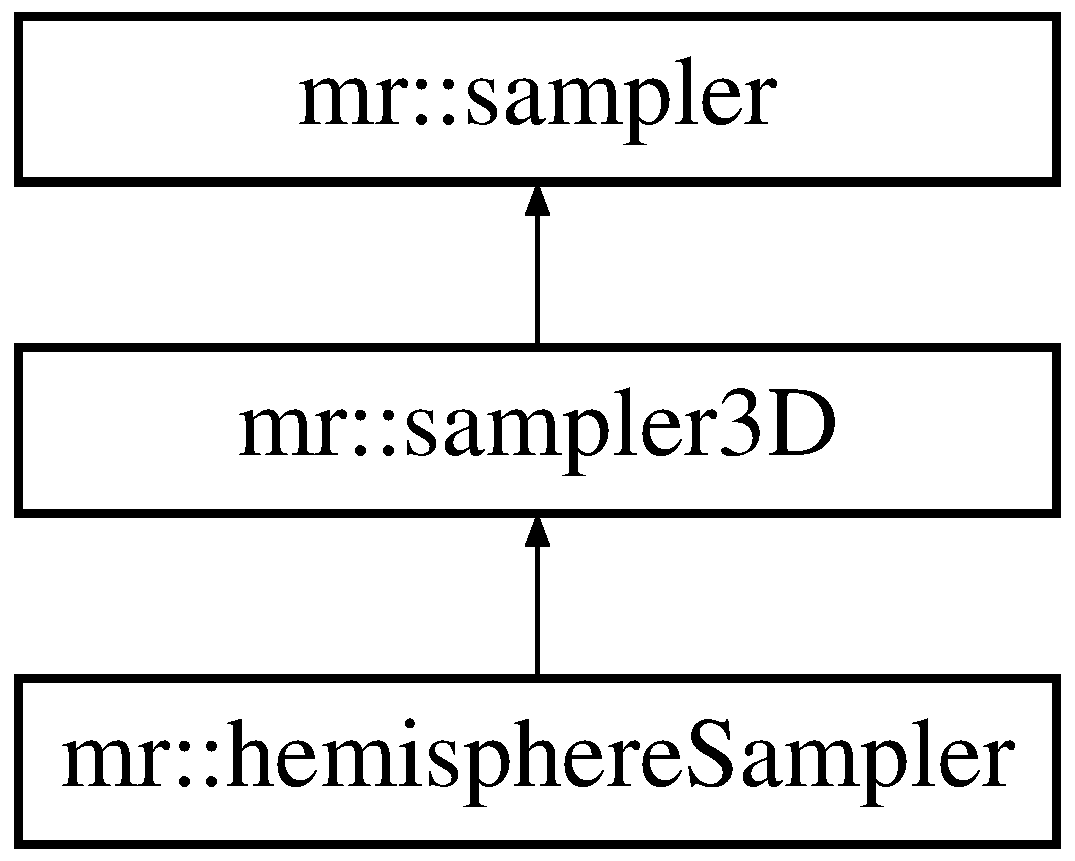
\includegraphics[height=3cm]{classmr_1_1hemisphereSampler}
\end{center}
\end{figure}
\subsection*{Public Member Functions}
\begin{CompactItemize}
\item 
{\bf hemisphere\-Sampler} (const mi\-Vector \&Nin)
\item 
{\bf hemisphere\-Sampler} (const mi\-Vector \&Nin, const mi\-Uint \&num\-Samples)
\item 
{\bf $\sim$hemisphere\-Sampler} ()
\item 
bool {\bf uniform} (const mi\-State $\ast$const state)
\item 
bool {\bf cosine} (const mi\-State $\ast$const state)
\item 
bool {\bf uniform} (const mi\-State $\ast$const state, const mi\-Scalar max)
\item 
bool {\bf cosine} (const mi\-State $\ast$const state, const mi\-Scalar max)
\item 
const mi\-Scalar {\bf weight} ()
\end{CompactItemize}
\subsection*{Protected Member Functions}
\begin{CompactItemize}
\item 
void {\bf UVNframe} ()
\item 
void {\bf cosine\-Distribution} ()
\item 
void {\bf cosine\-Distribution} (const mi\-Scalar max)
\item 
void {\bf uniform\-Distribution} ()
\item 
void {\bf uniform\-Distribution} (const mi\-Scalar max)
\item 
void {\bf calculate\-Direction} ()
\end{CompactItemize}


\subsection{Detailed Description}
Sample a full or partial hemisphere around a direction. 



\subsection{Constructor \& Destructor Documentation}
\index{mr::hemisphereSampler@{mr::hemisphere\-Sampler}!hemisphereSampler@{hemisphereSampler}}
\index{hemisphereSampler@{hemisphereSampler}!mr::hemisphereSampler@{mr::hemisphere\-Sampler}}
\subsubsection{\setlength{\rightskip}{0pt plus 5cm}mr::hemisphere\-Sampler::hemisphere\-Sampler (const mi\-Vector \& {\em Nin})\hspace{0.3cm}{\tt  [inline]}}\label{classmr_1_1hemisphereSampler_a0}


Constructor. Nin is the direction to sample around. sphere\-Percent is percentage of sphere to cover. This call is to be used when sampling adaptively (ie. the number of samples to be taken are not known or may vary, or you may exit the loop early). \index{mr::hemisphereSampler@{mr::hemisphere\-Sampler}!hemisphereSampler@{hemisphereSampler}}
\index{hemisphereSampler@{hemisphereSampler}!mr::hemisphereSampler@{mr::hemisphere\-Sampler}}
\subsubsection{\setlength{\rightskip}{0pt plus 5cm}mr::hemisphere\-Sampler::hemisphere\-Sampler (const mi\-Vector \& {\em Nin}, const mi\-Uint \& {\em num\-Samples})\hspace{0.3cm}{\tt  [inline]}}\label{classmr_1_1hemisphereSampler_a1}


Constructor. Nin is the direction to sample around. sphere\-Percent is percentage of sphere to cover. num\-Samples is the number of samples to take. It HAS to be mi\-Uint\& \index{mr::hemisphereSampler@{mr::hemisphere\-Sampler}!~hemisphereSampler@{$\sim$hemisphereSampler}}
\index{~hemisphereSampler@{$\sim$hemisphereSampler}!mr::hemisphereSampler@{mr::hemisphere\-Sampler}}
\subsubsection{\setlength{\rightskip}{0pt plus 5cm}mr::hemisphere\-Sampler::$\sim${\bf hemisphere\-Sampler} ()\hspace{0.3cm}{\tt  [inline]}}\label{classmr_1_1hemisphereSampler_a2}




\subsection{Member Function Documentation}
\index{mr::hemisphereSampler@{mr::hemisphere\-Sampler}!calculateDirection@{calculateDirection}}
\index{calculateDirection@{calculateDirection}!mr::hemisphereSampler@{mr::hemisphere\-Sampler}}
\subsubsection{\setlength{\rightskip}{0pt plus 5cm}void mr::hemisphere\-Sampler::calculate\-Direction ()\hspace{0.3cm}{\tt  [inline, protected]}}\label{classmr_1_1hemisphereSampler_b5}


\index{mr::hemisphereSampler@{mr::hemisphere\-Sampler}!cosine@{cosine}}
\index{cosine@{cosine}!mr::hemisphereSampler@{mr::hemisphere\-Sampler}}
\subsubsection{\setlength{\rightskip}{0pt plus 5cm}bool mr::hemisphere\-Sampler::cosine (const mi\-State $\ast$const {\em state}, const mi\-Scalar {\em max})\hspace{0.3cm}{\tt  [inline]}}\label{classmr_1_1hemisphereSampler_a6}


Get one sample using a cosine distribution over the max angle (expressed as a cosine [0,1]) or return false. \index{mr::hemisphereSampler@{mr::hemisphere\-Sampler}!cosine@{cosine}}
\index{cosine@{cosine}!mr::hemisphereSampler@{mr::hemisphere\-Sampler}}
\subsubsection{\setlength{\rightskip}{0pt plus 5cm}bool mr::hemisphere\-Sampler::cosine (const mi\-State $\ast$const {\em state})\hspace{0.3cm}{\tt  [inline]}}\label{classmr_1_1hemisphereSampler_a4}


Get one sample using a cosine distribution over the whole hemisphere or return false. \index{mr::hemisphereSampler@{mr::hemisphere\-Sampler}!cosineDistribution@{cosineDistribution}}
\index{cosineDistribution@{cosineDistribution}!mr::hemisphereSampler@{mr::hemisphere\-Sampler}}
\subsubsection{\setlength{\rightskip}{0pt plus 5cm}void mr::hemisphere\-Sampler::cosine\-Distribution (const mi\-Scalar {\em max})\hspace{0.3cm}{\tt  [inline, protected]}}\label{classmr_1_1hemisphereSampler_b2}


\index{mr::hemisphereSampler@{mr::hemisphere\-Sampler}!cosineDistribution@{cosineDistribution}}
\index{cosineDistribution@{cosineDistribution}!mr::hemisphereSampler@{mr::hemisphere\-Sampler}}
\subsubsection{\setlength{\rightskip}{0pt plus 5cm}void mr::hemisphere\-Sampler::cosine\-Distribution ()\hspace{0.3cm}{\tt  [inline, protected]}}\label{classmr_1_1hemisphereSampler_b1}


\index{mr::hemisphereSampler@{mr::hemisphere\-Sampler}!uniform@{uniform}}
\index{uniform@{uniform}!mr::hemisphereSampler@{mr::hemisphere\-Sampler}}
\subsubsection{\setlength{\rightskip}{0pt plus 5cm}bool mr::hemisphere\-Sampler::uniform (const mi\-State $\ast$const {\em state}, const mi\-Scalar {\em max})\hspace{0.3cm}{\tt  [inline]}}\label{classmr_1_1hemisphereSampler_a5}


Get one sample using a uniform distribution over the max angle (expressed as a cosine [0,1]) or return false. \index{mr::hemisphereSampler@{mr::hemisphere\-Sampler}!uniform@{uniform}}
\index{uniform@{uniform}!mr::hemisphereSampler@{mr::hemisphere\-Sampler}}
\subsubsection{\setlength{\rightskip}{0pt plus 5cm}bool mr::hemisphere\-Sampler::uniform (const mi\-State $\ast$const {\em state})\hspace{0.3cm}{\tt  [inline]}}\label{classmr_1_1hemisphereSampler_a3}


Get one sample using a uniform distribution over the whole hemisphere or return false. \index{mr::hemisphereSampler@{mr::hemisphere\-Sampler}!uniformDistribution@{uniformDistribution}}
\index{uniformDistribution@{uniformDistribution}!mr::hemisphereSampler@{mr::hemisphere\-Sampler}}
\subsubsection{\setlength{\rightskip}{0pt plus 5cm}void mr::hemisphere\-Sampler::uniform\-Distribution (const mi\-Scalar {\em max})\hspace{0.3cm}{\tt  [inline, protected]}}\label{classmr_1_1hemisphereSampler_b4}


\index{mr::hemisphereSampler@{mr::hemisphere\-Sampler}!uniformDistribution@{uniformDistribution}}
\index{uniformDistribution@{uniformDistribution}!mr::hemisphereSampler@{mr::hemisphere\-Sampler}}
\subsubsection{\setlength{\rightskip}{0pt plus 5cm}void mr::hemisphere\-Sampler::uniform\-Distribution ()\hspace{0.3cm}{\tt  [inline, protected]}}\label{classmr_1_1hemisphereSampler_b3}


\index{mr::hemisphereSampler@{mr::hemisphere\-Sampler}!UVNframe@{UVNframe}}
\index{UVNframe@{UVNframe}!mr::hemisphereSampler@{mr::hemisphere\-Sampler}}
\subsubsection{\setlength{\rightskip}{0pt plus 5cm}void mr::hemisphere\-Sampler::UVNframe ()\hspace{0.3cm}{\tt  [inline, protected]}}\label{classmr_1_1hemisphereSampler_b0}


\index{mr::hemisphereSampler@{mr::hemisphere\-Sampler}!weight@{weight}}
\index{weight@{weight}!mr::hemisphereSampler@{mr::hemisphere\-Sampler}}
\subsubsection{\setlength{\rightskip}{0pt plus 5cm}const mi\-Scalar mr::hemisphere\-Sampler::weight ()\hspace{0.3cm}{\tt  [inline]}}\label{classmr_1_1hemisphereSampler_a7}


This returns a weight (dot product) of the sample with respect to the original Nin vector. Useful in uniform distributions only. 

The documentation for this class was generated from the following file:\begin{CompactItemize}
\item 
{\bf mr\-Sampler.h}\end{CompactItemize}

\section{mr::infobuffer Struct Reference}
\label{structmr_1_1infobuffer}\index{mr::infobuffer@{mr::infobuffer}}
{\tt \#include $<$mr\-Stream.h$>$}

Inheritance diagram for mr::infobuffer::\begin{figure}[H]
\begin{center}
\leavevmode
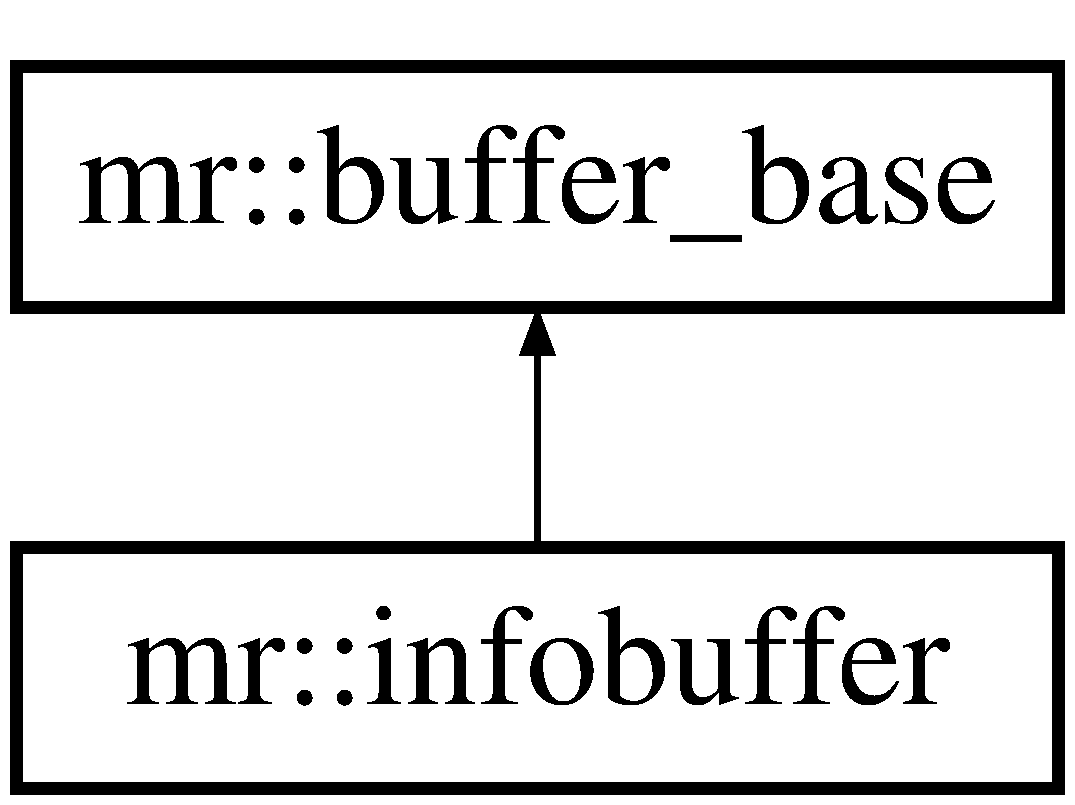
\includegraphics[height=2cm]{structmr_1_1infobuffer}
\end{center}
\end{figure}
\subsection*{Public Member Functions}
\begin{CompactItemize}
\item 
{\bf infobuffer} ()
\item 
virtual void {\bf print} (const char $\ast$const s)
\begin{CompactList}\small\item\em virtual function to print string out \item\end{CompactList}\end{CompactItemize}


\subsection{Detailed Description}
mental ray's printing out to console is based on old printf() syntax. This file uses some C++ wizardry to create some streams for printing out.

That is, instead of: mi\-Vector v; mi\_\-info(\char`\"{}[\%f, \%f, \%f] hello\char`\"{}, v.x, v.y, v.z);

you just can do: mr\_\-info( v $<$$<$ \char`\"{} hello\char`\"{} ); 



\subsection{Constructor \& Destructor Documentation}
\index{mr::infobuffer@{mr::infobuffer}!infobuffer@{infobuffer}}
\index{infobuffer@{infobuffer}!mr::infobuffer@{mr::infobuffer}}
\subsubsection{\setlength{\rightskip}{0pt plus 5cm}mr::infobuffer::infobuffer ()\hspace{0.3cm}{\tt  [inline]}}\label{structmr_1_1infobuffer_a0}




\subsection{Member Function Documentation}
\index{mr::infobuffer@{mr::infobuffer}!print@{print}}
\index{print@{print}!mr::infobuffer@{mr::infobuffer}}
\subsubsection{\setlength{\rightskip}{0pt plus 5cm}virtual void mr::infobuffer::print (const char $\ast$const {\em s})\hspace{0.3cm}{\tt  [inline, virtual]}}\label{structmr_1_1infobuffer_a1}


virtual function to print string out 



Implements {\bf mr::buffer\_\-base} {\rm (p.\,\pageref{structmr_1_1buffer__base_a3})}.

The documentation for this struct was generated from the following file:\begin{CompactItemize}
\item 
{\bf mr\-Stream.h}\end{CompactItemize}

\section{mr::infostream Struct Reference}
\label{structmr_1_1infostream}\index{mr::infostream@{mr::infostream}}
{\tt \#include $<$mr\-Stream.h$>$}

\subsection*{Public Member Functions}
\begin{CompactItemize}
\item 
{\bf infostream} ()
\item 
{\bf $\sim$infostream} ()
\end{CompactItemize}


\subsection{Constructor \& Destructor Documentation}
\index{mr::infostream@{mr::infostream}!infostream@{infostream}}
\index{infostream@{infostream}!mr::infostream@{mr::infostream}}
\subsubsection{\setlength{\rightskip}{0pt plus 5cm}mr::infostream::infostream ()\hspace{0.3cm}{\tt  [inline]}}\label{structmr_1_1infostream_a0}


\index{mr::infostream@{mr::infostream}!~infostream@{$\sim$infostream}}
\index{~infostream@{$\sim$infostream}!mr::infostream@{mr::infostream}}
\subsubsection{\setlength{\rightskip}{0pt plus 5cm}mr::infostream::$\sim${\bf infostream} ()\hspace{0.3cm}{\tt  [inline]}}\label{structmr_1_1infostream_a1}




The documentation for this struct was generated from the following file:\begin{CompactItemize}
\item 
{\bf mr\-Stream.h}\end{CompactItemize}

\section{interval$<$ T $>$ Class Template Reference}
\label{classinterval}\index{interval@{interval}}
{\tt \#include $<$mr\-Interval.h$>$}

\subsection*{Public Member Functions}
\begin{CompactItemize}
\item 
{\bf interval} ()
\item 
{\bf interval} (const T \&A, const T \&B)
\item 
bool {\bf operator==} (const {\bf interval}$<$ T $>$ \&src) const 
\item 
void {\bf make\-Empty} ()
\item 
void {\bf extend\-By} (const T \&point)
\item 
void {\bf extend\-By} (const {\bf interval}$<$ T $>$ \&b)
\item 
T {\bf size} () const 
\item 
T {\bf center} () const 
\item 
bool {\bf intersects} (const T \&point) const 
\item 
bool {\bf intersects} (const {\bf interval}$<$ T $>$ \&b) const 
\item 
bool {\bf has\-Volume} () const 
\item 
bool {\bf is\-Empty} () const 
\end{CompactItemize}
\subsubsection*{template$<$typename T$>$ class interval$<$ T $>$}



\subsection{Constructor \& Destructor Documentation}
\index{interval@{interval}!interval@{interval}}
\index{interval@{interval}!interval@{interval}}
\subsubsection{\setlength{\rightskip}{0pt plus 5cm}template$<$typename T$>$ {\bf interval}$<$ T $>$::{\bf interval} ()}\label{classinterval_a0}


\index{interval@{interval}!interval@{interval}}
\index{interval@{interval}!interval@{interval}}
\subsubsection{\setlength{\rightskip}{0pt plus 5cm}template$<$typename T$>$ {\bf interval}$<$ T $>$::{\bf interval} (const T \& {\em A}, const T \& {\em B})}\label{classinterval_a1}




\subsection{Member Function Documentation}
\index{interval@{interval}!center@{center}}
\index{center@{center}!interval@{interval}}
\subsubsection{\setlength{\rightskip}{0pt plus 5cm}template$<$typename T$>$ T {\bf interval}$<$ T $>$::center () const}\label{classinterval_a7}


\index{interval@{interval}!extendBy@{extendBy}}
\index{extendBy@{extendBy}!interval@{interval}}
\subsubsection{\setlength{\rightskip}{0pt plus 5cm}template$<$typename T$>$ void {\bf interval}$<$ T $>$::extend\-By (const {\bf interval}$<$ T $>$ \& {\em b})}\label{classinterval_a5}


\index{interval@{interval}!extendBy@{extendBy}}
\index{extendBy@{extendBy}!interval@{interval}}
\subsubsection{\setlength{\rightskip}{0pt plus 5cm}template$<$typename T$>$ void {\bf interval}$<$ T $>$::extend\-By (const T \& {\em point})}\label{classinterval_a4}


\index{interval@{interval}!hasVolume@{hasVolume}}
\index{hasVolume@{hasVolume}!interval@{interval}}
\subsubsection{\setlength{\rightskip}{0pt plus 5cm}template$<$typename T$>$ bool {\bf interval}$<$ T $>$::has\-Volume () const}\label{classinterval_a10}


\index{interval@{interval}!intersects@{intersects}}
\index{intersects@{intersects}!interval@{interval}}
\subsubsection{\setlength{\rightskip}{0pt plus 5cm}template$<$typename T$>$ bool {\bf interval}$<$ T $>$::intersects (const {\bf interval}$<$ T $>$ \& {\em b}) const}\label{classinterval_a9}


\index{interval@{interval}!intersects@{intersects}}
\index{intersects@{intersects}!interval@{interval}}
\subsubsection{\setlength{\rightskip}{0pt plus 5cm}template$<$typename T$>$ bool {\bf interval}$<$ T $>$::intersects (const T \& {\em point}) const}\label{classinterval_a8}


\index{interval@{interval}!isEmpty@{isEmpty}}
\index{isEmpty@{isEmpty}!interval@{interval}}
\subsubsection{\setlength{\rightskip}{0pt plus 5cm}template$<$typename T$>$ bool {\bf interval}$<$ T $>$::is\-Empty () const}\label{classinterval_a11}


\index{interval@{interval}!makeEmpty@{makeEmpty}}
\index{makeEmpty@{makeEmpty}!interval@{interval}}
\subsubsection{\setlength{\rightskip}{0pt plus 5cm}template$<$typename T$>$ void {\bf interval}$<$ T $>$::make\-Empty ()}\label{classinterval_a3}


\index{interval@{interval}!operator==@{operator==}}
\index{operator==@{operator==}!interval@{interval}}
\subsubsection{\setlength{\rightskip}{0pt plus 5cm}template$<$typename T$>$ bool {\bf interval}$<$ T $>$::operator== (const {\bf interval}$<$ T $>$ \& {\em src}) const}\label{classinterval_a2}


\index{interval@{interval}!size@{size}}
\index{size@{size}!interval@{interval}}
\subsubsection{\setlength{\rightskip}{0pt plus 5cm}template$<$typename T$>$ T {\bf interval}$<$ T $>$::size () const}\label{classinterval_a6}




The documentation for this class was generated from the following file:\begin{CompactItemize}
\item 
{\bf mr\-Interval.h}\end{CompactItemize}

\section{mr::less\-Tri\-Op Struct Reference}
\label{structmr_1_1lessTriOp}\index{mr::lessTriOp@{mr::lessTriOp}}
{\tt \#include $<$mr\-Functors.h$>$}

\subsection*{Public Member Functions}
\begin{CompactItemize}
\item 
template$<$typename T$>$ bool {\bf operator()} (const T \&a, const T \&b) const 
\end{CompactItemize}


\subsection{Detailed Description}
Functor class for sorting triangles based on pri and pri\_\-idx This is used for example as std::map$<$ tri\-Id, SOMETHING, less\-Tri\-Op $>$ or std::map$<$ mi\-State, SOMETHING, less\-Tri\-Op $>$ 



\subsection{Member Function Documentation}
\index{mr::lessTriOp@{mr::less\-Tri\-Op}!operator()@{operator()}}
\index{operator()@{operator()}!mr::lessTriOp@{mr::less\-Tri\-Op}}
\subsubsection{\setlength{\rightskip}{0pt plus 5cm}template$<$typename T$>$ bool mr::less\-Tri\-Op::operator() (const T \& {\em a}, const T \& {\em b}) const\hspace{0.3cm}{\tt  [inline]}}\label{structmr_1_1lessTriOp_a0}




The documentation for this struct was generated from the following file:\begin{CompactItemize}
\item 
{\bf mr\-Functors.h}\end{CompactItemize}

\section{mr::less\-UVOp Struct Reference}
\label{structmr_1_1lessUVOp}\index{mr::lessUVOp@{mr::lessUVOp}}
{\tt \#include $<$mr\-Functors.h$>$}

\subsection*{Public Member Functions}
\begin{CompactItemize}
\item 
template$<$typename T$>$ bool {\bf operator()} (const T \&a, const T \&b) const 
\end{CompactItemize}


\subsection{Detailed Description}
Functor class for sorting uv vectors This is used for example as std::map$<$ vector2d\-Type, SOMETHING, less\-UVOp $>$ 



\subsection{Member Function Documentation}
\index{mr::lessUVOp@{mr::less\-UVOp}!operator()@{operator()}}
\index{operator()@{operator()}!mr::lessUVOp@{mr::less\-UVOp}}
\subsubsection{\setlength{\rightskip}{0pt plus 5cm}template$<$typename T$>$ bool mr::less\-UVOp::operator() (const T \& {\em a}, const T \& {\em b}) const\hspace{0.3cm}{\tt  [inline]}}\label{structmr_1_1lessUVOp_a0}




The documentation for this struct was generated from the following file:\begin{CompactItemize}
\item 
{\bf mr\-Functors.h}\end{CompactItemize}

\section{mr::less\-XYZOp Struct Reference}
\label{structmr_1_1lessXYZOp}\index{mr::lessXYZOp@{mr::lessXYZOp}}
{\tt \#include $<$mr\-Functors.h$>$}

\subsection*{Public Member Functions}
\begin{CompactItemize}
\item 
template$<$typename T$>$ bool {\bf operator()} (const T \&a, const T \&b) const 
\end{CompactItemize}


\subsection{Detailed Description}
Functor class for sorting xyz vectors This is used for example as std::map$<$ vector\-Type, SOMETHING, less\-XYZOp $>$ 



\subsection{Member Function Documentation}
\index{mr::lessXYZOp@{mr::less\-XYZOp}!operator()@{operator()}}
\index{operator()@{operator()}!mr::lessXYZOp@{mr::less\-XYZOp}}
\subsubsection{\setlength{\rightskip}{0pt plus 5cm}template$<$typename T$>$ bool mr::less\-XYZOp::operator() (const T \& {\em a}, const T \& {\em b}) const\hspace{0.3cm}{\tt  [inline]}}\label{structmr_1_1lessXYZOp_a0}




The documentation for this struct was generated from the following file:\begin{CompactItemize}
\item 
{\bf mr\-Functors.h}\end{CompactItemize}

\section{mr::distances::Manhattan Struct Reference}
\label{structmr_1_1distances_1_1Manhattan}\index{mr::distances::Manhattan@{mr::distances::Manhattan}}
Functor to calculate manhattan distance.  


{\tt \#include $<$mr\-Distances.h$>$}

Inheritance diagram for mr::distances::Manhattan::\begin{figure}[H]
\begin{center}
\leavevmode
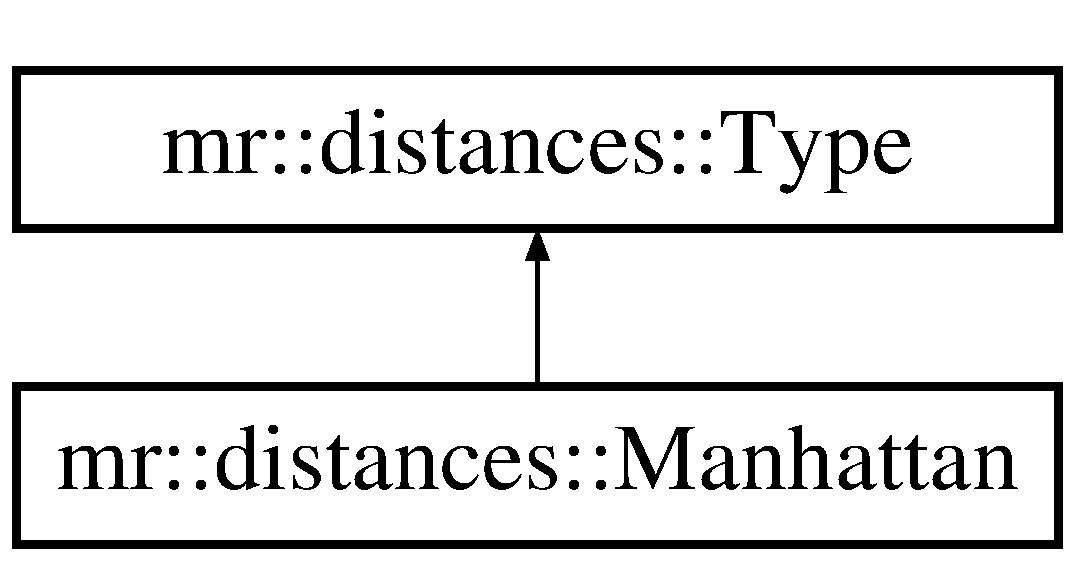
\includegraphics[height=2cm]{structmr_1_1distances_1_1Manhattan}
\end{center}
\end{figure}
\subsection*{Public Member Functions}
\begin{CompactItemize}
\item 
mi\-Scalar {\bf operator()} (const {\bf vector} \&d) const 
\item 
mi\-Scalar {\bf operator()} (const {\bf vector} \&d, const {\bf vector} \&s) const 
\end{CompactItemize}


\subsection{Detailed Description}
Functor to calculate manhattan distance. 



\subsection{Member Function Documentation}
\index{mr::distances::Manhattan@{mr::distances::Manhattan}!operator()@{operator()}}
\index{operator()@{operator()}!mr::distances::Manhattan@{mr::distances::Manhattan}}
\subsubsection{\setlength{\rightskip}{0pt plus 5cm}mi\-Scalar mr::distances::Manhattan::operator() (const {\bf vector} \& {\em d}, const {\bf vector} \& {\em s}) const\hspace{0.3cm}{\tt  [inline, virtual]}}\label{structmr_1_1distances_1_1Manhattan_a1}




Implements {\bf mr::distances::Type} {\rm (p.\,\pageref{structmr_1_1distances_1_1Type_a1})}.\index{mr::distances::Manhattan@{mr::distances::Manhattan}!operator()@{operator()}}
\index{operator()@{operator()}!mr::distances::Manhattan@{mr::distances::Manhattan}}
\subsubsection{\setlength{\rightskip}{0pt plus 5cm}mi\-Scalar mr::distances::Manhattan::operator() (const {\bf vector} \& {\em d}) const\hspace{0.3cm}{\tt  [inline, virtual]}}\label{structmr_1_1distances_1_1Manhattan_a0}




Implements {\bf mr::distances::Type} {\rm (p.\,\pageref{structmr_1_1distances_1_1Type_a0})}.

The documentation for this struct was generated from the following file:\begin{CompactItemize}
\item 
{\bf mr\-Distances.h}\end{CompactItemize}

\section{mr::math$<$ T $>$ Struct Template Reference}
\label{structmr_1_1math}\index{mr::math@{mr::math}}
{\tt \#include $<$mr\-Math.h$>$}

\subsection*{Static Public Member Functions}
\begin{CompactItemize}
\item 
T {\bf acos} (T x)
\item 
T {\bf asin} (T x)
\item 
T {\bf atan} (T x)
\item 
T {\bf atan2} (T x, T y)
\item 
T {\bf cos} (T x)
\item 
T {\bf sin} (T x)
\item 
T {\bf tan} (T x)
\item 
T {\bf cosh} (T x)
\item 
T {\bf sinh} (T x)
\item 
T {\bf tanh} (T x)
\item 
T {\bf exp} (T x)
\item 
T {\bf log} (T x)
\item 
T {\bf log10} (T x)
\item 
T {\bf modf} (T x, T $\ast$y)
\item 
T {\bf pow} (T x, T y)
\item 
T {\bf sqrt} (T x)
\item 
T {\bf ceil} (T x)
\item 
T {\bf fabs} (T x)
\item 
T {\bf floor} (T x)
\item 
T {\bf fmod} (T x, T y)
\item 
T {\bf hypot} (T x, T y)
\end{CompactItemize}
\subsubsection*{template$<$class T$>$ struct mr::math$<$ T $>$}



\subsection{Member Function Documentation}
\index{mr::math@{mr::math}!acos@{acos}}
\index{acos@{acos}!mr::math@{mr::math}}
\subsubsection{\setlength{\rightskip}{0pt plus 5cm}template$<$class T$>$ T {\bf mr::math}$<$ T $>$::acos (T {\em x})\hspace{0.3cm}{\tt  [inline, static]}}\label{structmr_1_1math_e0}


\index{mr::math@{mr::math}!asin@{asin}}
\index{asin@{asin}!mr::math@{mr::math}}
\subsubsection{\setlength{\rightskip}{0pt plus 5cm}template$<$class T$>$ T {\bf mr::math}$<$ T $>$::asin (T {\em x})\hspace{0.3cm}{\tt  [inline, static]}}\label{structmr_1_1math_e1}


\index{mr::math@{mr::math}!atan@{atan}}
\index{atan@{atan}!mr::math@{mr::math}}
\subsubsection{\setlength{\rightskip}{0pt plus 5cm}template$<$class T$>$ T {\bf mr::math}$<$ T $>$::atan (T {\em x})\hspace{0.3cm}{\tt  [inline, static]}}\label{structmr_1_1math_e2}


\index{mr::math@{mr::math}!atan2@{atan2}}
\index{atan2@{atan2}!mr::math@{mr::math}}
\subsubsection{\setlength{\rightskip}{0pt plus 5cm}template$<$class T$>$ T {\bf mr::math}$<$ T $>$::atan2 (T {\em x}, T {\em y})\hspace{0.3cm}{\tt  [inline, static]}}\label{structmr_1_1math_e3}


\index{mr::math@{mr::math}!ceil@{ceil}}
\index{ceil@{ceil}!mr::math@{mr::math}}
\subsubsection{\setlength{\rightskip}{0pt plus 5cm}template$<$class T$>$ T {\bf mr::math}$<$ T $>$::ceil (T {\em x})\hspace{0.3cm}{\tt  [inline, static]}}\label{structmr_1_1math_e16}


\index{mr::math@{mr::math}!cos@{cos}}
\index{cos@{cos}!mr::math@{mr::math}}
\subsubsection{\setlength{\rightskip}{0pt plus 5cm}template$<$class T$>$ T {\bf mr::math}$<$ T $>$::cos (T {\em x})\hspace{0.3cm}{\tt  [inline, static]}}\label{structmr_1_1math_e4}


\index{mr::math@{mr::math}!cosh@{cosh}}
\index{cosh@{cosh}!mr::math@{mr::math}}
\subsubsection{\setlength{\rightskip}{0pt plus 5cm}template$<$class T$>$ T {\bf mr::math}$<$ T $>$::cosh (T {\em x})\hspace{0.3cm}{\tt  [inline, static]}}\label{structmr_1_1math_e7}


\index{mr::math@{mr::math}!exp@{exp}}
\index{exp@{exp}!mr::math@{mr::math}}
\subsubsection{\setlength{\rightskip}{0pt plus 5cm}template$<$class T$>$ T {\bf mr::math}$<$ T $>$::exp (T {\em x})\hspace{0.3cm}{\tt  [inline, static]}}\label{structmr_1_1math_e10}


\index{mr::math@{mr::math}!fabs@{fabs}}
\index{fabs@{fabs}!mr::math@{mr::math}}
\subsubsection{\setlength{\rightskip}{0pt plus 5cm}template$<$class T$>$ T {\bf mr::math}$<$ T $>$::fabs (T {\em x})\hspace{0.3cm}{\tt  [inline, static]}}\label{structmr_1_1math_e17}


\index{mr::math@{mr::math}!floor@{floor}}
\index{floor@{floor}!mr::math@{mr::math}}
\subsubsection{\setlength{\rightskip}{0pt plus 5cm}template$<$class T$>$ T {\bf mr::math}$<$ T $>$::floor (T {\em x})\hspace{0.3cm}{\tt  [inline, static]}}\label{structmr_1_1math_e18}


\index{mr::math@{mr::math}!fmod@{fmod}}
\index{fmod@{fmod}!mr::math@{mr::math}}
\subsubsection{\setlength{\rightskip}{0pt plus 5cm}template$<$class T$>$ T {\bf mr::math}$<$ T $>$::fmod (T {\em x}, T {\em y})\hspace{0.3cm}{\tt  [inline, static]}}\label{structmr_1_1math_e19}


\index{mr::math@{mr::math}!hypot@{hypot}}
\index{hypot@{hypot}!mr::math@{mr::math}}
\subsubsection{\setlength{\rightskip}{0pt plus 5cm}template$<$class T$>$ T {\bf mr::math}$<$ T $>$::hypot (T {\em x}, T {\em y})\hspace{0.3cm}{\tt  [inline, static]}}\label{structmr_1_1math_e20}


\index{mr::math@{mr::math}!log@{log}}
\index{log@{log}!mr::math@{mr::math}}
\subsubsection{\setlength{\rightskip}{0pt plus 5cm}template$<$class T$>$ T {\bf mr::math}$<$ T $>$::log (T {\em x})\hspace{0.3cm}{\tt  [inline, static]}}\label{structmr_1_1math_e11}


\index{mr::math@{mr::math}!log10@{log10}}
\index{log10@{log10}!mr::math@{mr::math}}
\subsubsection{\setlength{\rightskip}{0pt plus 5cm}template$<$class T$>$ T {\bf mr::math}$<$ T $>$::log10 (T {\em x})\hspace{0.3cm}{\tt  [inline, static]}}\label{structmr_1_1math_e12}


\index{mr::math@{mr::math}!modf@{modf}}
\index{modf@{modf}!mr::math@{mr::math}}
\subsubsection{\setlength{\rightskip}{0pt plus 5cm}template$<$class T$>$ T {\bf mr::math}$<$ T $>$::modf (T {\em x}, T $\ast$ {\em y})\hspace{0.3cm}{\tt  [inline, static]}}\label{structmr_1_1math_e13}


\index{mr::math@{mr::math}!pow@{pow}}
\index{pow@{pow}!mr::math@{mr::math}}
\subsubsection{\setlength{\rightskip}{0pt plus 5cm}template$<$class T$>$ T {\bf mr::math}$<$ T $>$::pow (T {\em x}, T {\em y})\hspace{0.3cm}{\tt  [inline, static]}}\label{structmr_1_1math_e14}


\index{mr::math@{mr::math}!sin@{sin}}
\index{sin@{sin}!mr::math@{mr::math}}
\subsubsection{\setlength{\rightskip}{0pt plus 5cm}template$<$class T$>$ T {\bf mr::math}$<$ T $>$::sin (T {\em x})\hspace{0.3cm}{\tt  [inline, static]}}\label{structmr_1_1math_e5}


\index{mr::math@{mr::math}!sinh@{sinh}}
\index{sinh@{sinh}!mr::math@{mr::math}}
\subsubsection{\setlength{\rightskip}{0pt plus 5cm}template$<$class T$>$ T {\bf mr::math}$<$ T $>$::sinh (T {\em x})\hspace{0.3cm}{\tt  [inline, static]}}\label{structmr_1_1math_e8}


\index{mr::math@{mr::math}!sqrt@{sqrt}}
\index{sqrt@{sqrt}!mr::math@{mr::math}}
\subsubsection{\setlength{\rightskip}{0pt plus 5cm}template$<$class T$>$ T {\bf mr::math}$<$ T $>$::sqrt (T {\em x})\hspace{0.3cm}{\tt  [inline, static]}}\label{structmr_1_1math_e15}


\index{mr::math@{mr::math}!tan@{tan}}
\index{tan@{tan}!mr::math@{mr::math}}
\subsubsection{\setlength{\rightskip}{0pt plus 5cm}template$<$class T$>$ T {\bf mr::math}$<$ T $>$::tan (T {\em x})\hspace{0.3cm}{\tt  [inline, static]}}\label{structmr_1_1math_e6}


\index{mr::math@{mr::math}!tanh@{tanh}}
\index{tanh@{tanh}!mr::math@{mr::math}}
\subsubsection{\setlength{\rightskip}{0pt plus 5cm}template$<$class T$>$ T {\bf mr::math}$<$ T $>$::tanh (T {\em x})\hspace{0.3cm}{\tt  [inline, static]}}\label{structmr_1_1math_e9}




The documentation for this struct was generated from the following file:\begin{CompactItemize}
\item 
{\bf mr\-Math.h}\end{CompactItemize}

\section{mr::math$<$ float $>$ Struct Template Reference}
\label{structmr_1_1math_3_01float_01_4}\index{mr::math< float >@{mr::math$<$ float $>$}}
{\tt \#include $<$mr\-Math.h$>$}

\subsection*{Static Public Member Functions}
\begin{CompactItemize}
\item 
float {\bf acos} (float x)
\item 
float {\bf asin} (float x)
\item 
float {\bf atan} (float x)
\item 
float {\bf atan2} (float x, float y)
\item 
float {\bf cos} (float x)
\item 
float {\bf sin} (float x)
\item 
float {\bf tan} (float x)
\item 
float {\bf cosh} (float x)
\item 
float {\bf sinh} (float x)
\item 
float {\bf tanh} (float x)
\item 
float {\bf exp} (float x)
\item 
float {\bf log} (float x)
\item 
float {\bf log10} (float x)
\item 
float {\bf modf} (float x, float $\ast$y)
\item 
float {\bf pow} (float x, float y)
\item 
float {\bf sqrt} (float x)
\item 
float {\bf ceil} (float x)
\item 
float {\bf fabs} (float x)
\item 
float {\bf floor} (float x)
\item 
float {\bf fmod} (float x, float y)
\item 
float {\bf hypot} (float x, float y)
\end{CompactItemize}
\subsubsection*{template$<$$>$ struct mr::math$<$ float $>$}



\subsection{Member Function Documentation}
\index{mr::math< float >@{mr::math$<$ float $>$}!acos@{acos}}
\index{acos@{acos}!mr::math< float >@{mr::math$<$ float $>$}}
\subsubsection{\setlength{\rightskip}{0pt plus 5cm}float {\bf mr::math}$<$ float $>$::acos (float {\em x})\hspace{0.3cm}{\tt  [inline, static]}}\label{structmr_1_1math_3_01float_01_4_e0}


\index{mr::math< float >@{mr::math$<$ float $>$}!asin@{asin}}
\index{asin@{asin}!mr::math< float >@{mr::math$<$ float $>$}}
\subsubsection{\setlength{\rightskip}{0pt plus 5cm}float {\bf mr::math}$<$ float $>$::asin (float {\em x})\hspace{0.3cm}{\tt  [inline, static]}}\label{structmr_1_1math_3_01float_01_4_e1}


\index{mr::math< float >@{mr::math$<$ float $>$}!atan@{atan}}
\index{atan@{atan}!mr::math< float >@{mr::math$<$ float $>$}}
\subsubsection{\setlength{\rightskip}{0pt plus 5cm}float {\bf mr::math}$<$ float $>$::atan (float {\em x})\hspace{0.3cm}{\tt  [inline, static]}}\label{structmr_1_1math_3_01float_01_4_e2}


\index{mr::math< float >@{mr::math$<$ float $>$}!atan2@{atan2}}
\index{atan2@{atan2}!mr::math< float >@{mr::math$<$ float $>$}}
\subsubsection{\setlength{\rightskip}{0pt plus 5cm}float {\bf mr::math}$<$ float $>$::atan2 (float {\em x}, float {\em y})\hspace{0.3cm}{\tt  [inline, static]}}\label{structmr_1_1math_3_01float_01_4_e3}


\index{mr::math< float >@{mr::math$<$ float $>$}!ceil@{ceil}}
\index{ceil@{ceil}!mr::math< float >@{mr::math$<$ float $>$}}
\subsubsection{\setlength{\rightskip}{0pt plus 5cm}float {\bf mr::math}$<$ float $>$::ceil (float {\em x})\hspace{0.3cm}{\tt  [inline, static]}}\label{structmr_1_1math_3_01float_01_4_e16}


\index{mr::math< float >@{mr::math$<$ float $>$}!cos@{cos}}
\index{cos@{cos}!mr::math< float >@{mr::math$<$ float $>$}}
\subsubsection{\setlength{\rightskip}{0pt plus 5cm}float {\bf mr::math}$<$ float $>$::cos (float {\em x})\hspace{0.3cm}{\tt  [inline, static]}}\label{structmr_1_1math_3_01float_01_4_e4}


\index{mr::math< float >@{mr::math$<$ float $>$}!cosh@{cosh}}
\index{cosh@{cosh}!mr::math< float >@{mr::math$<$ float $>$}}
\subsubsection{\setlength{\rightskip}{0pt plus 5cm}float {\bf mr::math}$<$ float $>$::cosh (float {\em x})\hspace{0.3cm}{\tt  [inline, static]}}\label{structmr_1_1math_3_01float_01_4_e7}


\index{mr::math< float >@{mr::math$<$ float $>$}!exp@{exp}}
\index{exp@{exp}!mr::math< float >@{mr::math$<$ float $>$}}
\subsubsection{\setlength{\rightskip}{0pt plus 5cm}float {\bf mr::math}$<$ float $>$::exp (float {\em x})\hspace{0.3cm}{\tt  [inline, static]}}\label{structmr_1_1math_3_01float_01_4_e10}


\index{mr::math< float >@{mr::math$<$ float $>$}!fabs@{fabs}}
\index{fabs@{fabs}!mr::math< float >@{mr::math$<$ float $>$}}
\subsubsection{\setlength{\rightskip}{0pt plus 5cm}float {\bf mr::math}$<$ float $>$::fabs (float {\em x})\hspace{0.3cm}{\tt  [inline, static]}}\label{structmr_1_1math_3_01float_01_4_e17}


\index{mr::math< float >@{mr::math$<$ float $>$}!floor@{floor}}
\index{floor@{floor}!mr::math< float >@{mr::math$<$ float $>$}}
\subsubsection{\setlength{\rightskip}{0pt plus 5cm}float {\bf mr::math}$<$ float $>$::floor (float {\em x})\hspace{0.3cm}{\tt  [inline, static]}}\label{structmr_1_1math_3_01float_01_4_e18}


\index{mr::math< float >@{mr::math$<$ float $>$}!fmod@{fmod}}
\index{fmod@{fmod}!mr::math< float >@{mr::math$<$ float $>$}}
\subsubsection{\setlength{\rightskip}{0pt plus 5cm}float {\bf mr::math}$<$ float $>$::fmod (float {\em x}, float {\em y})\hspace{0.3cm}{\tt  [inline, static]}}\label{structmr_1_1math_3_01float_01_4_e19}


\index{mr::math< float >@{mr::math$<$ float $>$}!hypot@{hypot}}
\index{hypot@{hypot}!mr::math< float >@{mr::math$<$ float $>$}}
\subsubsection{\setlength{\rightskip}{0pt plus 5cm}float {\bf mr::math}$<$ float $>$::hypot (float {\em x}, float {\em y})\hspace{0.3cm}{\tt  [inline, static]}}\label{structmr_1_1math_3_01float_01_4_e20}


\index{mr::math< float >@{mr::math$<$ float $>$}!log@{log}}
\index{log@{log}!mr::math< float >@{mr::math$<$ float $>$}}
\subsubsection{\setlength{\rightskip}{0pt plus 5cm}float {\bf mr::math}$<$ float $>$::log (float {\em x})\hspace{0.3cm}{\tt  [inline, static]}}\label{structmr_1_1math_3_01float_01_4_e11}


\index{mr::math< float >@{mr::math$<$ float $>$}!log10@{log10}}
\index{log10@{log10}!mr::math< float >@{mr::math$<$ float $>$}}
\subsubsection{\setlength{\rightskip}{0pt plus 5cm}float {\bf mr::math}$<$ float $>$::log10 (float {\em x})\hspace{0.3cm}{\tt  [inline, static]}}\label{structmr_1_1math_3_01float_01_4_e12}


\index{mr::math< float >@{mr::math$<$ float $>$}!modf@{modf}}
\index{modf@{modf}!mr::math< float >@{mr::math$<$ float $>$}}
\subsubsection{\setlength{\rightskip}{0pt plus 5cm}float {\bf mr::math}$<$ float $>$::modf (float {\em x}, float $\ast$ {\em y})\hspace{0.3cm}{\tt  [inline, static]}}\label{structmr_1_1math_3_01float_01_4_e13}


\index{mr::math< float >@{mr::math$<$ float $>$}!pow@{pow}}
\index{pow@{pow}!mr::math< float >@{mr::math$<$ float $>$}}
\subsubsection{\setlength{\rightskip}{0pt plus 5cm}float {\bf mr::math}$<$ float $>$::pow (float {\em x}, float {\em y})\hspace{0.3cm}{\tt  [inline, static]}}\label{structmr_1_1math_3_01float_01_4_e14}


\index{mr::math< float >@{mr::math$<$ float $>$}!sin@{sin}}
\index{sin@{sin}!mr::math< float >@{mr::math$<$ float $>$}}
\subsubsection{\setlength{\rightskip}{0pt plus 5cm}float {\bf mr::math}$<$ float $>$::sin (float {\em x})\hspace{0.3cm}{\tt  [inline, static]}}\label{structmr_1_1math_3_01float_01_4_e5}


\index{mr::math< float >@{mr::math$<$ float $>$}!sinh@{sinh}}
\index{sinh@{sinh}!mr::math< float >@{mr::math$<$ float $>$}}
\subsubsection{\setlength{\rightskip}{0pt plus 5cm}float {\bf mr::math}$<$ float $>$::sinh (float {\em x})\hspace{0.3cm}{\tt  [inline, static]}}\label{structmr_1_1math_3_01float_01_4_e8}


\index{mr::math< float >@{mr::math$<$ float $>$}!sqrt@{sqrt}}
\index{sqrt@{sqrt}!mr::math< float >@{mr::math$<$ float $>$}}
\subsubsection{\setlength{\rightskip}{0pt plus 5cm}float {\bf mr::math}$<$ float $>$::sqrt (float {\em x})\hspace{0.3cm}{\tt  [inline, static]}}\label{structmr_1_1math_3_01float_01_4_e15}


\index{mr::math< float >@{mr::math$<$ float $>$}!tan@{tan}}
\index{tan@{tan}!mr::math< float >@{mr::math$<$ float $>$}}
\subsubsection{\setlength{\rightskip}{0pt plus 5cm}float {\bf mr::math}$<$ float $>$::tan (float {\em x})\hspace{0.3cm}{\tt  [inline, static]}}\label{structmr_1_1math_3_01float_01_4_e6}


\index{mr::math< float >@{mr::math$<$ float $>$}!tanh@{tanh}}
\index{tanh@{tanh}!mr::math< float >@{mr::math$<$ float $>$}}
\subsubsection{\setlength{\rightskip}{0pt plus 5cm}float {\bf mr::math}$<$ float $>$::tanh (float {\em x})\hspace{0.3cm}{\tt  [inline, static]}}\label{structmr_1_1math_3_01float_01_4_e9}




The documentation for this struct was generated from the following file:\begin{CompactItemize}
\item 
{\bf mr\-Math.h}\end{CompactItemize}

\section{mr::matrix Class Reference}
\label{classmr_1_1matrix}\index{mr::matrix@{mr::matrix}}
Class to represent a matrix in mental ray.  


{\tt \#include $<$mr\-Matrix.h$>$}

\subsection*{Enumerations}
\begin{CompactItemize}
\item 
enum {\bf Matrix\-Type} \{ \par
{\bf k\-Empty} =  0, 
{\bf k\-Identity}, 
{\bf k\-Internal\-To\-World}, 
{\bf k\-Internal\-To\-Camera}, 
\par
{\bf k\-Internal\-To\-Object}, 
{\bf k\-Camera\-To\-World}, 
{\bf k\-Camera\-To\-Object}, 
{\bf k\-Camera\-To\-Internal}, 
\par
{\bf k\-Camera\-Projection}, 
{\bf k\-Object\-To\-World}, 
{\bf k\-Object\-To\-Internal}, 
{\bf k\-Object\-To\-Camera}, 
\par
{\bf k\-Unknown}
 \}
\begin{CompactList}\small\item\em Default matrices. \item\end{CompactList}\item 
void {\bf set\-To\-Null} ()
\begin{CompactList}\small\item\em Set Matrix all to 0. \item\end{CompactList}\item 
void {\bf set\-To\-Identity} ()
\begin{CompactList}\small\item\em Set Matrix to Identity. \item\end{CompactList}\item 
void {\bf set\-Internal\-To\-World} (mi\-State $\ast$const state)
\begin{CompactList}\small\item\em Set Matrix to Internal-$>$World Matrix. \item\end{CompactList}\item 
void {\bf set\-Internal\-To\-Camera} (mi\-State $\ast$const state)
\begin{CompactList}\small\item\em Set Matrix to Internal-$>$Camera Matrix. \item\end{CompactList}\item 
void {\bf set\-Internal\-To\-Object} (mi\-State $\ast$const state)
\begin{CompactList}\small\item\em Set Matrix to Internal-$>$Object Matrix. \item\end{CompactList}\item 
void {\bf set\-Camera\-To\-World} (mi\-State $\ast$const state)
\begin{CompactList}\small\item\em Set Matrix to Camera-$>$World Matrix. \item\end{CompactList}\item 
void {\bf set\-Camera\-To\-Internal} (mi\-State $\ast$const state)
\begin{CompactList}\small\item\em Set Matrix to Camera-$>$Internal Matrix. \item\end{CompactList}\item 
void {\bf set\-Object\-To\-World} (mi\-State $\ast$const state)
\begin{CompactList}\small\item\em Set Matrix to Object-$>$World Matrix. \item\end{CompactList}\item 
void {\bf set\-Object\-To\-Internal} (mi\-State $\ast$const state)
\begin{CompactList}\small\item\em Set Matrix to Object-$>$Internal Matrix. \item\end{CompactList}\item 
void {\bf set\-Camera\-To\-Object} (mi\-State $\ast$const state)
\begin{CompactList}\small\item\em Set Matrix to Camera-$>$Object Matrix. \item\end{CompactList}\item 
void {\bf set\-Object\-To\-Camera} (mi\-State $\ast$const state)
\begin{CompactList}\small\item\em Set Matrix to Object-$>$Camera Matrix. \item\end{CompactList}\end{CompactItemize}
\subsection*{Friend operators}
\begin{CompactItemize}
\item 
std::ostream \& {\bf operator$<$$<$} (std::ostream \&o, const {\bf matrix} \&a)
\begin{CompactList}\small\item\em Printing. \item\end{CompactList}\item 
{\bf matrix} {\bf operator $\ast$} (const mi\-Scalar scalar, const {\bf matrix} \&b)
\begin{CompactList}\small\item\em Reverse scalar multiplication. \item\end{CompactList}\end{CompactItemize}
\subsection*{Public Types}
\subsection*{Public Member Functions}
\begin{Indent}{\bf Constructors}\par
\begin{CompactItemize}
\item 
{\bf matrix} ({\bf k\-No\-Construct})
\begin{CompactList}\small\item\em Quick Constructor. Leaves matrix elements unitialized. \item\end{CompactList}\item 
{\bf matrix} ()
\begin{CompactList}\small\item\em Default Constructor. Sets matrix to identity. \item\end{CompactList}\item 
{\bf matrix} (const mi\-Matrix m)
\begin{CompactList}\small\item\em Construct matrix from an mi\-Matrix. \item\end{CompactList}\item 
{\bf matrix} (mi\-State $\ast$const state, const {\bf Matrix\-Type} n)
\begin{CompactList}\small\item\em Construct matrix from a default matrix. \item\end{CompactList}\item 
{\bf matrix} (const mi\-Integer n)
\begin{CompactList}\small\item\em Construct matrix from an Integer (this is same as prman 0=null, 1=identity). \item\end{CompactList}\item 
{\bf matrix} (const {\bf Matrix\-Type} n)
\begin{CompactList}\small\item\em Construct matrix from a default matrix (only valid for identity/null). \item\end{CompactList}\item 
{\bf matrix} (const mi\-Scalar m00, const mi\-Scalar m01, const mi\-Scalar m02, const mi\-Scalar m10, const mi\-Scalar m11, const mi\-Scalar m12, const mi\-Scalar m20, const mi\-Scalar m21, const mi\-Scalar m22)
\begin{CompactList}\small\item\em Construct matrix from 9 scalars for a non-perspective matrix. \item\end{CompactList}\item 
{\bf matrix} (const mi\-Scalar m00, const mi\-Scalar m01, const mi\-Scalar m02, const mi\-Scalar m03, const mi\-Scalar m10, const mi\-Scalar m11, const mi\-Scalar m12, const mi\-Scalar m13, const mi\-Scalar m20, const mi\-Scalar m21, const mi\-Scalar m22, const mi\-Scalar m23, const mi\-Scalar m30, const mi\-Scalar m31, const mi\-Scalar m32, const mi\-Scalar m33)
\begin{CompactList}\small\item\em Construct matrix from 16 scalars for a perspective matrix. \item\end{CompactList}\item 
{\bf matrix} (const mi\-Scalar f[4][4])
\begin{CompactList}\small\item\em Construct matrix from an array of 4x4 scalars. \item\end{CompactList}\item 
{\bf matrix} (const mi\-State $\ast$const state)
\begin{CompactList}\small\item\em Construct matrix as a projection from camera data in mi\-State. \item\end{CompactList}\item 
{\bf matrix} (const {\bf matrix} \&a)
\begin{CompactList}\small\item\em Copy Constructor. \item\end{CompactList}\item 
{\bf $\sim$matrix} ()
\begin{CompactList}\small\item\em Destructor. \item\end{CompactList}\end{CompactItemize}
\end{Indent}
\begin{Indent}{\bf Comparison functions}\par
\begin{CompactItemize}
\item 
bool {\bf is\-Null} () const 
\begin{CompactList}\small\item\em Is matrix the null matrix? \item\end{CompactList}\item 
bool {\bf is\-Identity} () const 
\begin{CompactList}\small\item\em Is matrix the identity matrix? \item\end{CompactList}\end{CompactItemize}
\end{Indent}
\begin{Indent}{\bf Assignment}\par
\begin{CompactItemize}
\item 
{\bf matrix} \& {\bf operator=} (const mi\-Matrix a)
\begin{CompactList}\small\item\em Assign a new mi\-Matrix. \item\end{CompactList}\item 
{\bf matrix} \& {\bf operator=} (const {\bf matrix} \&a)
\begin{CompactList}\small\item\em Assign a new matrix. \item\end{CompactList}\item 
{\bf matrix} \& {\bf operator=} (const mi\-Integer a)
\begin{CompactList}\small\item\em Assign a new matrix from default matrices (0=null,1=identity). \item\end{CompactList}\item 
{\bf matrix} \& {\bf operator=} (const {\bf Matrix\-Type} a)
\begin{CompactList}\small\item\em Assign a new matrix from default matrices. \item\end{CompactList}\end{CompactItemize}
\end{Indent}
\begin{Indent}{\bf Accesors}\par
\begin{CompactItemize}
\item 
mi\-Scalar $\ast$ {\bf operator \&} () const 
\begin{CompactList}\small\item\em Access matrix pointer (useful to pass to mray functions). \item\end{CompactList}\item 
const mi\-Scalar $\ast$ {\bf operator[$\,$]} (const unsigned row) const 
\begin{CompactList}\small\item\em Access a specific row of matrix for reading. \item\end{CompactList}\item 
mi\-Scalar $\ast$ {\bf operator[$\,$]} (const unsigned row)
\begin{CompactList}\small\item\em Access a specific row of matrix for assignment. \item\end{CompactList}\item 
mi\-Scalar {\bf get} (const unsigned idx) const 
\begin{CompactList}\small\item\em Access a specific index[0,15] of matrix for reading. \item\end{CompactList}\item 
void {\bf set} (const unsigned idx, const mi\-Scalar s)
\begin{CompactList}\small\item\em Access a specific index[0,15] of matrix for assignment. \item\end{CompactList}\end{CompactItemize}
\end{Indent}
\begin{Indent}{\bf Operations}\par
\begin{CompactItemize}
\item 
{\bf matrix} {\bf transposed} () const 
\item 
const {\bf matrix} \& {\bf transpose} ()
\begin{CompactList}\small\item\em Transpose of this matrix in place. \item\end{CompactList}\item 
{\bf matrix} {\bf inverse} () const 
\item 
const {\bf matrix} \& {\bf invert} ()
\begin{CompactList}\small\item\em Invert this matrix in place. \item\end{CompactList}\item 
{\bf matrix} {\bf adjoint} () const 
\begin{CompactList}\small\item\em Return the adjoint matrix. \item\end{CompactList}\item 
mi\-Scalar {\bf det4x4} () const 
\begin{CompactList}\small\item\em Return the 4x4 determinant. \item\end{CompactList}\item 
const {\bf matrix} \& {\bf transpose3x3} ()
\item 
{\bf matrix} {\bf transposed3x3} () const 
\item 
{\bf matrix} {\bf inverse3x3} () const 
\item 
const {\bf matrix} \& {\bf invert3x3} ()
\begin{CompactList}\small\item\em Invert this matrix in place. Inverts as if 3x3 matrix. \item\end{CompactList}\item 
{\bf matrix} {\bf adjoint3x3} () const 
\begin{CompactList}\small\item\em Return the adjoint matrix, assuming matrix is 3x3. \item\end{CompactList}\item 
mi\-Scalar {\bf det3x3} () const 
\begin{CompactList}\small\item\em Return the 3x3 determinant. \item\end{CompactList}\item 
void {\bf orthographic} (const mi\-Scalar near\_\-plane=0.0f, const mi\-Scalar far\_\-plane=1.0f, const mi\-Scalar left\_\-plane=-1.0f, const mi\-Scalar right\_\-plane=1.0f, const mi\-Scalar top\_\-plane=1.0f, const mi\-Scalar bottom\_\-plane=-1.0f)
\begin{CompactList}\small\item\em Creates a projection matrix (ortho). \item\end{CompactList}\item 
void {\bf orthographic} (const mi\-State $\ast$const state)
\begin{CompactList}\small\item\em Creates an orthographi matrix matching camera's. \item\end{CompactList}\item 
void {\bf projection} (const mi\-State $\ast$const state)
\begin{CompactList}\small\item\em Creates a projection matrix (frustrum) matching camera's. \item\end{CompactList}\item 
void {\bf projection} (const mi\-Scalar near\_\-plane=0.0f, const mi\-Scalar far\_\-plane=1.0f, const mi\-Scalar left\_\-plane=-1.0f, const mi\-Scalar right\_\-plane=1.0f, const mi\-Scalar top\_\-plane=1.0f, const mi\-Scalar bottom\_\-plane=-1.0f)
\begin{CompactList}\small\item\em Creates a projection matrix (frustrum). \item\end{CompactList}\item 
void {\bf translate} (const mi\-Scalar x, const mi\-Scalar y, const mi\-Scalar z)
\begin{CompactList}\small\item\em Add an xyz translation to the matrix. \item\end{CompactList}\item 
void {\bf translate} (const mi\-Vector v)
\begin{CompactList}\small\item\em Add an xyz translation to the matrix. \item\end{CompactList}\item 
void {\bf rotate} (const mi\-Scalar x, const mi\-Scalar y, const mi\-Scalar z)
\begin{CompactList}\small\item\em Add an xyz euler rotation to the matrix. \item\end{CompactList}\item 
void {\bf rotate} (const mi\-Vector v)
\begin{CompactList}\small\item\em Add an xyz euler rotation to the matrix. \item\end{CompactList}\item 
void {\bf scale} (const mi\-Scalar x, const mi\-Scalar y, const mi\-Scalar z)
\begin{CompactList}\small\item\em Add an xyz scaling to the matrix. \item\end{CompactList}\item 
void {\bf scale} (const mi\-Scalar xyz)
\begin{CompactList}\small\item\em Add a proportional scaling to the matrix. \item\end{CompactList}\item 
void {\bf scale} (const mi\-Vector \&v)
\begin{CompactList}\small\item\em Add an xyz scaling to the matrix. \item\end{CompactList}\item 
bool {\bf operator!=} (const {\bf matrix} \&a) const 
\begin{CompactList}\small\item\em Per component, check for inequality. \item\end{CompactList}\item 
bool {\bf operator==} (const {\bf matrix} \&a) const 
\begin{CompactList}\small\item\em Per component, check for equality. \item\end{CompactList}\item 
{\bf matrix} \& {\bf operator+=} (const {\bf matrix} \&a)
\begin{CompactList}\small\item\em Per component sum. \item\end{CompactList}\item 
{\bf matrix} \& {\bf operator+=} (const mi\-Matrix a)
\begin{CompactList}\small\item\em Per component sum. \item\end{CompactList}\item 
{\bf matrix} \& {\bf operator-=} (const {\bf matrix} \&a)
\begin{CompactList}\small\item\em Per component substraction. \item\end{CompactList}\item 
{\bf matrix} \& {\bf operator-=} (const mi\-Matrix a)
\begin{CompactList}\small\item\em Per component substraction. \item\end{CompactList}\item 
{\bf matrix} \& {\bf operator $\ast$=} (const mi\-Scalar scalar)
\begin{CompactList}\small\item\em Scalar multiplication. \item\end{CompactList}\item 
{\bf matrix} \& {\bf operator $\ast$=} (const {\bf matrix} \&a)
\begin{CompactList}\small\item\em Matrix post-multiplication. \item\end{CompactList}\item 
{\bf matrix} \& {\bf operator $\ast$=} (const mi\-Matrix a)
\begin{CompactList}\small\item\em Matrix post-multiplication. \item\end{CompactList}\item 
{\bf matrix} \& {\bf operator/=} (const mi\-Scalar scalar)
\begin{CompactList}\small\item\em Scalar division. \item\end{CompactList}\item 
{\bf matrix} \& {\bf operator/=} (const {\bf matrix} \&a)
\begin{CompactList}\small\item\em Matrix post-multiplication of the inverse of a matrix. \item\end{CompactList}\item 
{\bf matrix} \& {\bf operator/=} (const mi\-Matrix a)
\begin{CompactList}\small\item\em Matrix post-multiplication of the inverse of a matrix. \item\end{CompactList}\item 
{\bf matrix} {\bf operator-} () const 
\begin{CompactList}\small\item\em Negation. \item\end{CompactList}\item 
{\bf matrix} {\bf operator+} (const mi\-Matrix b) const 
\begin{CompactList}\small\item\em Per component sum. \item\end{CompactList}\item 
{\bf matrix} {\bf operator+} (const {\bf matrix} \&b) const 
\begin{CompactList}\small\item\em Per component sum. \item\end{CompactList}\item 
{\bf matrix} {\bf operator-} (const mi\-Matrix b) const 
\begin{CompactList}\small\item\em Per component substraction. \item\end{CompactList}\item 
{\bf matrix} {\bf operator-} (const {\bf matrix} \&b) const 
\begin{CompactList}\small\item\em Per component substraction. \item\end{CompactList}\item 
{\bf matrix} {\bf operator $\ast$} (const mi\-Scalar scalar) const 
\begin{CompactList}\small\item\em Scalar multiplication. \item\end{CompactList}\item 
{\bf matrix} {\bf operator $\ast$} (const mi\-Matrix b) const 
\begin{CompactList}\small\item\em Matrix post-multiplication. \item\end{CompactList}\item 
{\bf matrix} {\bf operator $\ast$} (const {\bf matrix} \&b) const 
\begin{CompactList}\small\item\em Matrix post-multiplication. \item\end{CompactList}\item 
{\bf matrix} {\bf operator/} (const mi\-Scalar scalar) const 
\begin{CompactList}\small\item\em Scalar division. \item\end{CompactList}\item 
{\bf matrix} {\bf operator/} (const mi\-Matrix b) const 
\begin{CompactList}\small\item\em Matrix post-multiplication of the inverse of a matrix. \item\end{CompactList}\item 
{\bf matrix} {\bf operator/} (const {\bf matrix} \&b) const 
\begin{CompactList}\small\item\em Matrix post-multiplication of the inverse of a matrix. \item\end{CompactList}\end{CompactItemize}
\end{Indent}


\subsection{Detailed Description}
Class to represent a matrix in mental ray. 



\subsection{Member Enumeration Documentation}
\index{mr::matrix@{mr::matrix}!MatrixType@{MatrixType}}
\index{MatrixType@{MatrixType}!mr::matrix@{mr::matrix}}
\subsubsection{\setlength{\rightskip}{0pt plus 5cm}enum {\bf mr::matrix::Matrix\-Type}}\label{classmr_1_1matrix_z18_0}


Default matrices. 

\begin{Desc}
\item[Enumeration values: ]\par
\begin{description}
\index{kEmpty@{kEmpty}!mr::matrix@{mr::matrix}}\index{mr::matrix@{mr::matrix}!kEmpty@{kEmpty}}\item[{\em 
k\-Empty\label{classmr_1_1matrix_z18_0w0}
}]\index{kIdentity@{kIdentity}!mr::matrix@{mr::matrix}}\index{mr::matrix@{mr::matrix}!kIdentity@{kIdentity}}\item[{\em 
k\-Identity\label{classmr_1_1matrix_z18_0w1}
}]\index{kInternalToWorld@{kInternalToWorld}!mr::matrix@{mr::matrix}}\index{mr::matrix@{mr::matrix}!kInternalToWorld@{kInternalToWorld}}\item[{\em 
k\-Internal\-To\-World\label{classmr_1_1matrix_z18_0w2}
}]\index{kInternalToCamera@{kInternalToCamera}!mr::matrix@{mr::matrix}}\index{mr::matrix@{mr::matrix}!kInternalToCamera@{kInternalToCamera}}\item[{\em 
k\-Internal\-To\-Camera\label{classmr_1_1matrix_z18_0w3}
}]\index{kInternalToObject@{kInternalToObject}!mr::matrix@{mr::matrix}}\index{mr::matrix@{mr::matrix}!kInternalToObject@{kInternalToObject}}\item[{\em 
k\-Internal\-To\-Object\label{classmr_1_1matrix_z18_0w4}
}]\index{kCameraToWorld@{kCameraToWorld}!mr::matrix@{mr::matrix}}\index{mr::matrix@{mr::matrix}!kCameraToWorld@{kCameraToWorld}}\item[{\em 
k\-Camera\-To\-World\label{classmr_1_1matrix_z18_0w5}
}]\index{kCameraToObject@{kCameraToObject}!mr::matrix@{mr::matrix}}\index{mr::matrix@{mr::matrix}!kCameraToObject@{kCameraToObject}}\item[{\em 
k\-Camera\-To\-Object\label{classmr_1_1matrix_z18_0w6}
}]\index{kCameraToInternal@{kCameraToInternal}!mr::matrix@{mr::matrix}}\index{mr::matrix@{mr::matrix}!kCameraToInternal@{kCameraToInternal}}\item[{\em 
k\-Camera\-To\-Internal\label{classmr_1_1matrix_z18_0w7}
}]\index{kCameraProjection@{kCameraProjection}!mr::matrix@{mr::matrix}}\index{mr::matrix@{mr::matrix}!kCameraProjection@{kCameraProjection}}\item[{\em 
k\-Camera\-Projection\label{classmr_1_1matrix_z18_0w8}
}]\index{kObjectToWorld@{kObjectToWorld}!mr::matrix@{mr::matrix}}\index{mr::matrix@{mr::matrix}!kObjectToWorld@{kObjectToWorld}}\item[{\em 
k\-Object\-To\-World\label{classmr_1_1matrix_z18_0w9}
}]\index{kObjectToInternal@{kObjectToInternal}!mr::matrix@{mr::matrix}}\index{mr::matrix@{mr::matrix}!kObjectToInternal@{kObjectToInternal}}\item[{\em 
k\-Object\-To\-Internal\label{classmr_1_1matrix_z18_0w10}
}]\index{kObjectToCamera@{kObjectToCamera}!mr::matrix@{mr::matrix}}\index{mr::matrix@{mr::matrix}!kObjectToCamera@{kObjectToCamera}}\item[{\em 
k\-Object\-To\-Camera\label{classmr_1_1matrix_z18_0w11}
}]\index{kUnknown@{kUnknown}!mr::matrix@{mr::matrix}}\index{mr::matrix@{mr::matrix}!kUnknown@{kUnknown}}\item[{\em 
k\-Unknown\label{classmr_1_1matrix_z18_0w12}
}]\end{description}
\end{Desc}



\subsection{Constructor \& Destructor Documentation}
\index{mr::matrix@{mr::matrix}!matrix@{matrix}}
\index{matrix@{matrix}!mr::matrix@{mr::matrix}}
\subsubsection{\setlength{\rightskip}{0pt plus 5cm}mr::matrix::matrix ({\bf k\-No\-Construct})\hspace{0.3cm}{\tt  [inline]}}\label{classmr_1_1matrix_z19_0}


Quick Constructor. Leaves matrix elements unitialized. 

\index{mr::matrix@{mr::matrix}!matrix@{matrix}}
\index{matrix@{matrix}!mr::matrix@{mr::matrix}}
\subsubsection{\setlength{\rightskip}{0pt plus 5cm}mr::matrix::matrix ()\hspace{0.3cm}{\tt  [inline]}}\label{classmr_1_1matrix_z19_1}


Default Constructor. Sets matrix to identity. 

\index{mr::matrix@{mr::matrix}!matrix@{matrix}}
\index{matrix@{matrix}!mr::matrix@{mr::matrix}}
\subsubsection{\setlength{\rightskip}{0pt plus 5cm}mr::matrix::matrix (const mi\-Matrix {\em m})\hspace{0.3cm}{\tt  [inline]}}\label{classmr_1_1matrix_z19_2}


Construct matrix from an mi\-Matrix. 

\index{mr::matrix@{mr::matrix}!matrix@{matrix}}
\index{matrix@{matrix}!mr::matrix@{mr::matrix}}
\subsubsection{\setlength{\rightskip}{0pt plus 5cm}mr::matrix::matrix (mi\-State $\ast$const {\em state}, const {\bf Matrix\-Type} {\em n})\hspace{0.3cm}{\tt  [inline]}}\label{classmr_1_1matrix_z19_3}


Construct matrix from a default matrix. 

\index{mr::matrix@{mr::matrix}!matrix@{matrix}}
\index{matrix@{matrix}!mr::matrix@{mr::matrix}}
\subsubsection{\setlength{\rightskip}{0pt plus 5cm}mr::matrix::matrix (const mi\-Integer {\em n})\hspace{0.3cm}{\tt  [inline]}}\label{classmr_1_1matrix_z19_4}


Construct matrix from an Integer (this is same as prman 0=null, 1=identity). 

\index{mr::matrix@{mr::matrix}!matrix@{matrix}}
\index{matrix@{matrix}!mr::matrix@{mr::matrix}}
\subsubsection{\setlength{\rightskip}{0pt plus 5cm}mr::matrix::matrix (const {\bf Matrix\-Type} {\em n})\hspace{0.3cm}{\tt  [inline]}}\label{classmr_1_1matrix_z19_5}


Construct matrix from a default matrix (only valid for identity/null). 

\index{mr::matrix@{mr::matrix}!matrix@{matrix}}
\index{matrix@{matrix}!mr::matrix@{mr::matrix}}
\subsubsection{\setlength{\rightskip}{0pt plus 5cm}mr::matrix::matrix (const mi\-Scalar {\em m00}, const mi\-Scalar {\em m01}, const mi\-Scalar {\em m02}, const mi\-Scalar {\em m10}, const mi\-Scalar {\em m11}, const mi\-Scalar {\em m12}, const mi\-Scalar {\em m20}, const mi\-Scalar {\em m21}, const mi\-Scalar {\em m22})\hspace{0.3cm}{\tt  [inline]}}\label{classmr_1_1matrix_z19_6}


Construct matrix from 9 scalars for a non-perspective matrix. 

\index{mr::matrix@{mr::matrix}!matrix@{matrix}}
\index{matrix@{matrix}!mr::matrix@{mr::matrix}}
\subsubsection{\setlength{\rightskip}{0pt plus 5cm}mr::matrix::matrix (const mi\-Scalar {\em m00}, const mi\-Scalar {\em m01}, const mi\-Scalar {\em m02}, const mi\-Scalar {\em m03}, const mi\-Scalar {\em m10}, const mi\-Scalar {\em m11}, const mi\-Scalar {\em m12}, const mi\-Scalar {\em m13}, const mi\-Scalar {\em m20}, const mi\-Scalar {\em m21}, const mi\-Scalar {\em m22}, const mi\-Scalar {\em m23}, const mi\-Scalar {\em m30}, const mi\-Scalar {\em m31}, const mi\-Scalar {\em m32}, const mi\-Scalar {\em m33})\hspace{0.3cm}{\tt  [inline]}}\label{classmr_1_1matrix_z19_7}


Construct matrix from 16 scalars for a perspective matrix. 

\index{mr::matrix@{mr::matrix}!matrix@{matrix}}
\index{matrix@{matrix}!mr::matrix@{mr::matrix}}
\subsubsection{\setlength{\rightskip}{0pt plus 5cm}mr::matrix::matrix (const mi\-Scalar {\em f}[4][4])\hspace{0.3cm}{\tt  [inline]}}\label{classmr_1_1matrix_z19_8}


Construct matrix from an array of 4x4 scalars. 

\index{mr::matrix@{mr::matrix}!matrix@{matrix}}
\index{matrix@{matrix}!mr::matrix@{mr::matrix}}
\subsubsection{\setlength{\rightskip}{0pt plus 5cm}mr::matrix::matrix (const mi\-State $\ast$const {\em state})\hspace{0.3cm}{\tt  [inline]}}\label{classmr_1_1matrix_z19_9}


Construct matrix as a projection from camera data in mi\-State. 

\index{mr::matrix@{mr::matrix}!matrix@{matrix}}
\index{matrix@{matrix}!mr::matrix@{mr::matrix}}
\subsubsection{\setlength{\rightskip}{0pt plus 5cm}mr::matrix::matrix (const {\bf matrix} \& {\em a})\hspace{0.3cm}{\tt  [inline]}}\label{classmr_1_1matrix_z19_10}


Copy Constructor. 

\index{mr::matrix@{mr::matrix}!~matrix@{$\sim$matrix}}
\index{~matrix@{$\sim$matrix}!mr::matrix@{mr::matrix}}
\subsubsection{\setlength{\rightskip}{0pt plus 5cm}mr::matrix::$\sim${\bf matrix} ()\hspace{0.3cm}{\tt  [inline]}}\label{classmr_1_1matrix_z19_11}


Destructor. 



\subsection{Member Function Documentation}
\index{mr::matrix@{mr::matrix}!adjoint@{adjoint}}
\index{adjoint@{adjoint}!mr::matrix@{mr::matrix}}
\subsubsection{\setlength{\rightskip}{0pt plus 5cm}{\bf matrix} mr::matrix::adjoint () const\hspace{0.3cm}{\tt  [inline]}}\label{classmr_1_1matrix_z23_4}


Return the adjoint matrix. 

\index{mr::matrix@{mr::matrix}!adjoint3x3@{adjoint3x3}}
\index{adjoint3x3@{adjoint3x3}!mr::matrix@{mr::matrix}}
\subsubsection{\setlength{\rightskip}{0pt plus 5cm}{\bf matrix} mr::matrix::adjoint3x3 () const\hspace{0.3cm}{\tt  [inline]}}\label{classmr_1_1matrix_z23_10}


Return the adjoint matrix, assuming matrix is 3x3. 

\index{mr::matrix@{mr::matrix}!det3x3@{det3x3}}
\index{det3x3@{det3x3}!mr::matrix@{mr::matrix}}
\subsubsection{\setlength{\rightskip}{0pt plus 5cm}mi\-Scalar mr::matrix::det3x3 () const\hspace{0.3cm}{\tt  [inline]}}\label{classmr_1_1matrix_z23_11}


Return the 3x3 determinant. 

\index{mr::matrix@{mr::matrix}!det4x4@{det4x4}}
\index{det4x4@{det4x4}!mr::matrix@{mr::matrix}}
\subsubsection{\setlength{\rightskip}{0pt plus 5cm}mi\-Scalar mr::matrix::det4x4 () const\hspace{0.3cm}{\tt  [inline]}}\label{classmr_1_1matrix_z23_5}


Return the 4x4 determinant. 

\index{mr::matrix@{mr::matrix}!get@{get}}
\index{get@{get}!mr::matrix@{mr::matrix}}
\subsubsection{\setlength{\rightskip}{0pt plus 5cm}mi\-Scalar mr::matrix::get (const unsigned {\em idx}) const\hspace{0.3cm}{\tt  [inline]}}\label{classmr_1_1matrix_z22_3}


Access a specific index[0,15] of matrix for reading. 

\index{mr::matrix@{mr::matrix}!inverse@{inverse}}
\index{inverse@{inverse}!mr::matrix@{mr::matrix}}
\subsubsection{\setlength{\rightskip}{0pt plus 5cm}{\bf matrix} mr::matrix::inverse () const\hspace{0.3cm}{\tt  [inline]}}\label{classmr_1_1matrix_z23_2}


Return the inverse of this matrix. Does not modify the original. \index{mr::matrix@{mr::matrix}!inverse3x3@{inverse3x3}}
\index{inverse3x3@{inverse3x3}!mr::matrix@{mr::matrix}}
\subsubsection{\setlength{\rightskip}{0pt plus 5cm}{\bf matrix} mr::matrix::inverse3x3 () const\hspace{0.3cm}{\tt  [inline]}}\label{classmr_1_1matrix_z23_8}


Return the inverse of this matrix. Does not modify the original. Assumes matrix is 3x3 and other rows/cols are untouched \index{mr::matrix@{mr::matrix}!invert@{invert}}
\index{invert@{invert}!mr::matrix@{mr::matrix}}
\subsubsection{\setlength{\rightskip}{0pt plus 5cm}const {\bf matrix}\& mr::matrix::invert ()\hspace{0.3cm}{\tt  [inline]}}\label{classmr_1_1matrix_z23_3}


Invert this matrix in place. 

\index{mr::matrix@{mr::matrix}!invert3x3@{invert3x3}}
\index{invert3x3@{invert3x3}!mr::matrix@{mr::matrix}}
\subsubsection{\setlength{\rightskip}{0pt plus 5cm}const {\bf matrix}\& mr::matrix::invert3x3 ()\hspace{0.3cm}{\tt  [inline]}}\label{classmr_1_1matrix_z23_9}


Invert this matrix in place. Inverts as if 3x3 matrix. 

\index{mr::matrix@{mr::matrix}!isIdentity@{isIdentity}}
\index{isIdentity@{isIdentity}!mr::matrix@{mr::matrix}}
\subsubsection{\setlength{\rightskip}{0pt plus 5cm}bool mr::matrix::is\-Identity () const\hspace{0.3cm}{\tt  [inline]}}\label{classmr_1_1matrix_z20_1}


Is matrix the identity matrix? 

\index{mr::matrix@{mr::matrix}!isNull@{isNull}}
\index{isNull@{isNull}!mr::matrix@{mr::matrix}}
\subsubsection{\setlength{\rightskip}{0pt plus 5cm}bool mr::matrix::is\-Null () const\hspace{0.3cm}{\tt  [inline]}}\label{classmr_1_1matrix_z20_0}


Is matrix the null matrix? 

\index{mr::matrix@{mr::matrix}!operator &@{operator \&}}
\index{operator &@{operator \&}!mr::matrix@{mr::matrix}}
\subsubsection{\setlength{\rightskip}{0pt plus 5cm}mi\-Scalar$\ast$ mr::matrix::operator \& () const\hspace{0.3cm}{\tt  [inline]}}\label{classmr_1_1matrix_z22_0}


Access matrix pointer (useful to pass to mray functions). 

\index{mr::matrix@{mr::matrix}!operator *@{operator $\ast$}}
\index{operator *@{operator $\ast$}!mr::matrix@{mr::matrix}}
\subsubsection{\setlength{\rightskip}{0pt plus 5cm}{\bf matrix} mr::matrix::operator $\ast$ (const {\bf matrix} \& {\em b}) const\hspace{0.3cm}{\tt  [inline]}}\label{classmr_1_1matrix_z23_42}


Matrix post-multiplication. 

\index{mr::matrix@{mr::matrix}!operator *@{operator $\ast$}}
\index{operator *@{operator $\ast$}!mr::matrix@{mr::matrix}}
\subsubsection{\setlength{\rightskip}{0pt plus 5cm}{\bf matrix} mr::matrix::operator $\ast$ (const mi\-Matrix {\em b}) const\hspace{0.3cm}{\tt  [inline]}}\label{classmr_1_1matrix_z23_41}


Matrix post-multiplication. 

\index{mr::matrix@{mr::matrix}!operator *@{operator $\ast$}}
\index{operator *@{operator $\ast$}!mr::matrix@{mr::matrix}}
\subsubsection{\setlength{\rightskip}{0pt plus 5cm}{\bf matrix} mr::matrix::operator $\ast$ (const mi\-Scalar {\em scalar}) const\hspace{0.3cm}{\tt  [inline]}}\label{classmr_1_1matrix_z23_40}


Scalar multiplication. 

\index{mr::matrix@{mr::matrix}!operator *=@{operator $\ast$=}}
\index{operator *=@{operator $\ast$=}!mr::matrix@{mr::matrix}}
\subsubsection{\setlength{\rightskip}{0pt plus 5cm}{\bf matrix}\& mr::matrix::operator $\ast$= (const mi\-Matrix {\em a})\hspace{0.3cm}{\tt  [inline]}}\label{classmr_1_1matrix_z23_31}


Matrix post-multiplication. 

\index{mr::matrix@{mr::matrix}!operator *=@{operator $\ast$=}}
\index{operator *=@{operator $\ast$=}!mr::matrix@{mr::matrix}}
\subsubsection{\setlength{\rightskip}{0pt plus 5cm}{\bf matrix}\& mr::matrix::operator $\ast$= (const {\bf matrix} \& {\em a})\hspace{0.3cm}{\tt  [inline]}}\label{classmr_1_1matrix_z23_30}


Matrix post-multiplication. 

\index{mr::matrix@{mr::matrix}!operator *=@{operator $\ast$=}}
\index{operator *=@{operator $\ast$=}!mr::matrix@{mr::matrix}}
\subsubsection{\setlength{\rightskip}{0pt plus 5cm}{\bf matrix}\& mr::matrix::operator $\ast$= (const mi\-Scalar {\em scalar})\hspace{0.3cm}{\tt  [inline]}}\label{classmr_1_1matrix_z23_29}


Scalar multiplication. 

\index{mr::matrix@{mr::matrix}!operator"!=@{operator"!=}}
\index{operator"!=@{operator"!=}!mr::matrix@{mr::matrix}}
\subsubsection{\setlength{\rightskip}{0pt plus 5cm}bool mr::matrix::operator!= (const {\bf matrix} \& {\em a}) const\hspace{0.3cm}{\tt  [inline]}}\label{classmr_1_1matrix_z23_23}


Per component, check for inequality. 

\index{mr::matrix@{mr::matrix}!operator+@{operator+}}
\index{operator+@{operator+}!mr::matrix@{mr::matrix}}
\subsubsection{\setlength{\rightskip}{0pt plus 5cm}{\bf matrix} mr::matrix::operator+ (const {\bf matrix} \& {\em b}) const\hspace{0.3cm}{\tt  [inline]}}\label{classmr_1_1matrix_z23_37}


Per component sum. 

\index{mr::matrix@{mr::matrix}!operator+@{operator+}}
\index{operator+@{operator+}!mr::matrix@{mr::matrix}}
\subsubsection{\setlength{\rightskip}{0pt plus 5cm}{\bf matrix} mr::matrix::operator+ (const mi\-Matrix {\em b}) const\hspace{0.3cm}{\tt  [inline]}}\label{classmr_1_1matrix_z23_36}


Per component sum. 

\index{mr::matrix@{mr::matrix}!operator+=@{operator+=}}
\index{operator+=@{operator+=}!mr::matrix@{mr::matrix}}
\subsubsection{\setlength{\rightskip}{0pt plus 5cm}{\bf matrix}\& mr::matrix::operator+= (const mi\-Matrix {\em a})\hspace{0.3cm}{\tt  [inline]}}\label{classmr_1_1matrix_z23_26}


Per component sum. 

\index{mr::matrix@{mr::matrix}!operator+=@{operator+=}}
\index{operator+=@{operator+=}!mr::matrix@{mr::matrix}}
\subsubsection{\setlength{\rightskip}{0pt plus 5cm}{\bf matrix}\& mr::matrix::operator+= (const {\bf matrix} \& {\em a})\hspace{0.3cm}{\tt  [inline]}}\label{classmr_1_1matrix_z23_25}


Per component sum. 

\index{mr::matrix@{mr::matrix}!operator-@{operator-}}
\index{operator-@{operator-}!mr::matrix@{mr::matrix}}
\subsubsection{\setlength{\rightskip}{0pt plus 5cm}{\bf matrix} mr::matrix::operator- (const {\bf matrix} \& {\em b}) const\hspace{0.3cm}{\tt  [inline]}}\label{classmr_1_1matrix_z23_39}


Per component substraction. 

\index{mr::matrix@{mr::matrix}!operator-@{operator-}}
\index{operator-@{operator-}!mr::matrix@{mr::matrix}}
\subsubsection{\setlength{\rightskip}{0pt plus 5cm}{\bf matrix} mr::matrix::operator- (const mi\-Matrix {\em b}) const\hspace{0.3cm}{\tt  [inline]}}\label{classmr_1_1matrix_z23_38}


Per component substraction. 

\index{mr::matrix@{mr::matrix}!operator-@{operator-}}
\index{operator-@{operator-}!mr::matrix@{mr::matrix}}
\subsubsection{\setlength{\rightskip}{0pt plus 5cm}{\bf matrix} mr::matrix::operator- () const\hspace{0.3cm}{\tt  [inline]}}\label{classmr_1_1matrix_z23_35}


Negation. 

\index{mr::matrix@{mr::matrix}!operator-=@{operator-=}}
\index{operator-=@{operator-=}!mr::matrix@{mr::matrix}}
\subsubsection{\setlength{\rightskip}{0pt plus 5cm}{\bf matrix}\& mr::matrix::operator-= (const mi\-Matrix {\em a})\hspace{0.3cm}{\tt  [inline]}}\label{classmr_1_1matrix_z23_28}


Per component substraction. 

\index{mr::matrix@{mr::matrix}!operator-=@{operator-=}}
\index{operator-=@{operator-=}!mr::matrix@{mr::matrix}}
\subsubsection{\setlength{\rightskip}{0pt plus 5cm}{\bf matrix}\& mr::matrix::operator-= (const {\bf matrix} \& {\em a})\hspace{0.3cm}{\tt  [inline]}}\label{classmr_1_1matrix_z23_27}


Per component substraction. 

\index{mr::matrix@{mr::matrix}!operator/@{operator/}}
\index{operator/@{operator/}!mr::matrix@{mr::matrix}}
\subsubsection{\setlength{\rightskip}{0pt plus 5cm}{\bf matrix} mr::matrix::operator/ (const {\bf matrix} \& {\em b}) const\hspace{0.3cm}{\tt  [inline]}}\label{classmr_1_1matrix_z23_45}


Matrix post-multiplication of the inverse of a matrix. 

\index{mr::matrix@{mr::matrix}!operator/@{operator/}}
\index{operator/@{operator/}!mr::matrix@{mr::matrix}}
\subsubsection{\setlength{\rightskip}{0pt plus 5cm}{\bf matrix} mr::matrix::operator/ (const mi\-Matrix {\em b}) const\hspace{0.3cm}{\tt  [inline]}}\label{classmr_1_1matrix_z23_44}


Matrix post-multiplication of the inverse of a matrix. 

\index{mr::matrix@{mr::matrix}!operator/@{operator/}}
\index{operator/@{operator/}!mr::matrix@{mr::matrix}}
\subsubsection{\setlength{\rightskip}{0pt plus 5cm}{\bf matrix} mr::matrix::operator/ (const mi\-Scalar {\em scalar}) const\hspace{0.3cm}{\tt  [inline]}}\label{classmr_1_1matrix_z23_43}


Scalar division. 

\index{mr::matrix@{mr::matrix}!operator/=@{operator/=}}
\index{operator/=@{operator/=}!mr::matrix@{mr::matrix}}
\subsubsection{\setlength{\rightskip}{0pt plus 5cm}{\bf matrix}\& mr::matrix::operator/= (const mi\-Matrix {\em a})\hspace{0.3cm}{\tt  [inline]}}\label{classmr_1_1matrix_z23_34}


Matrix post-multiplication of the inverse of a matrix. 

\index{mr::matrix@{mr::matrix}!operator/=@{operator/=}}
\index{operator/=@{operator/=}!mr::matrix@{mr::matrix}}
\subsubsection{\setlength{\rightskip}{0pt plus 5cm}{\bf matrix}\& mr::matrix::operator/= (const {\bf matrix} \& {\em a})\hspace{0.3cm}{\tt  [inline]}}\label{classmr_1_1matrix_z23_33}


Matrix post-multiplication of the inverse of a matrix. 

\index{mr::matrix@{mr::matrix}!operator/=@{operator/=}}
\index{operator/=@{operator/=}!mr::matrix@{mr::matrix}}
\subsubsection{\setlength{\rightskip}{0pt plus 5cm}{\bf matrix}\& mr::matrix::operator/= (const mi\-Scalar {\em scalar})\hspace{0.3cm}{\tt  [inline]}}\label{classmr_1_1matrix_z23_32}


Scalar division. 

\index{mr::matrix@{mr::matrix}!operator=@{operator=}}
\index{operator=@{operator=}!mr::matrix@{mr::matrix}}
\subsubsection{\setlength{\rightskip}{0pt plus 5cm}{\bf matrix}\& mr::matrix::operator= (const {\bf Matrix\-Type} {\em a})\hspace{0.3cm}{\tt  [inline]}}\label{classmr_1_1matrix_z21_3}


Assign a new matrix from default matrices. 

\index{mr::matrix@{mr::matrix}!operator=@{operator=}}
\index{operator=@{operator=}!mr::matrix@{mr::matrix}}
\subsubsection{\setlength{\rightskip}{0pt plus 5cm}{\bf matrix}\& mr::matrix::operator= (const mi\-Integer {\em a})\hspace{0.3cm}{\tt  [inline]}}\label{classmr_1_1matrix_z21_2}


Assign a new matrix from default matrices (0=null,1=identity). 

\index{mr::matrix@{mr::matrix}!operator=@{operator=}}
\index{operator=@{operator=}!mr::matrix@{mr::matrix}}
\subsubsection{\setlength{\rightskip}{0pt plus 5cm}{\bf matrix}\& mr::matrix::operator= (const {\bf matrix} \& {\em a})\hspace{0.3cm}{\tt  [inline]}}\label{classmr_1_1matrix_z21_1}


Assign a new matrix. 

\index{mr::matrix@{mr::matrix}!operator=@{operator=}}
\index{operator=@{operator=}!mr::matrix@{mr::matrix}}
\subsubsection{\setlength{\rightskip}{0pt plus 5cm}{\bf matrix}\& mr::matrix::operator= (const mi\-Matrix {\em a})\hspace{0.3cm}{\tt  [inline]}}\label{classmr_1_1matrix_z21_0}


Assign a new mi\-Matrix. 

\index{mr::matrix@{mr::matrix}!operator==@{operator==}}
\index{operator==@{operator==}!mr::matrix@{mr::matrix}}
\subsubsection{\setlength{\rightskip}{0pt plus 5cm}bool mr::matrix::operator== (const {\bf matrix} \& {\em a}) const\hspace{0.3cm}{\tt  [inline]}}\label{classmr_1_1matrix_z23_24}


Per component, check for equality. 

\index{mr::matrix@{mr::matrix}!operator[]@{operator[]}}
\index{operator[]@{operator[]}!mr::matrix@{mr::matrix}}
\subsubsection{\setlength{\rightskip}{0pt plus 5cm}mi\-Scalar$\ast$ mr::matrix::operator[$\,$] (const unsigned {\em row})\hspace{0.3cm}{\tt  [inline]}}\label{classmr_1_1matrix_z22_2}


Access a specific row of matrix for assignment. 

\index{mr::matrix@{mr::matrix}!operator[]@{operator[]}}
\index{operator[]@{operator[]}!mr::matrix@{mr::matrix}}
\subsubsection{\setlength{\rightskip}{0pt plus 5cm}const mi\-Scalar$\ast$ mr::matrix::operator[$\,$] (const unsigned {\em row}) const\hspace{0.3cm}{\tt  [inline]}}\label{classmr_1_1matrix_z22_1}


Access a specific row of matrix for reading. 

\index{mr::matrix@{mr::matrix}!orthographic@{orthographic}}
\index{orthographic@{orthographic}!mr::matrix@{mr::matrix}}
\subsubsection{\setlength{\rightskip}{0pt plus 5cm}void mr::matrix::orthographic (const mi\-State $\ast$const {\em state})\hspace{0.3cm}{\tt  [inline]}}\label{classmr_1_1matrix_z23_13}


Creates an orthographi matrix matching camera's. 

\index{mr::matrix@{mr::matrix}!orthographic@{orthographic}}
\index{orthographic@{orthographic}!mr::matrix@{mr::matrix}}
\subsubsection{\setlength{\rightskip}{0pt plus 5cm}void mr::matrix::orthographic (const mi\-Scalar {\em near\_\-plane} = 0.0f, const mi\-Scalar {\em far\_\-plane} = 1.0f, const mi\-Scalar {\em left\_\-plane} = -1.0f, const mi\-Scalar {\em right\_\-plane} = 1.0f, const mi\-Scalar {\em top\_\-plane} = 1.0f, const mi\-Scalar {\em bottom\_\-plane} = -1.0f)\hspace{0.3cm}{\tt  [inline]}}\label{classmr_1_1matrix_z23_12}


Creates a projection matrix (ortho). 

\index{mr::matrix@{mr::matrix}!projection@{projection}}
\index{projection@{projection}!mr::matrix@{mr::matrix}}
\subsubsection{\setlength{\rightskip}{0pt plus 5cm}void mr::matrix::projection (const mi\-Scalar {\em near\_\-plane} = 0.0f, const mi\-Scalar {\em far\_\-plane} = 1.0f, const mi\-Scalar {\em left\_\-plane} = -1.0f, const mi\-Scalar {\em right\_\-plane} = 1.0f, const mi\-Scalar {\em top\_\-plane} = 1.0f, const mi\-Scalar {\em bottom\_\-plane} = -1.0f)\hspace{0.3cm}{\tt  [inline]}}\label{classmr_1_1matrix_z23_15}


Creates a projection matrix (frustrum). 

\index{mr::matrix@{mr::matrix}!projection@{projection}}
\index{projection@{projection}!mr::matrix@{mr::matrix}}
\subsubsection{\setlength{\rightskip}{0pt plus 5cm}void mr::matrix::projection (const mi\-State $\ast$const {\em state})\hspace{0.3cm}{\tt  [inline]}}\label{classmr_1_1matrix_z23_14}


Creates a projection matrix (frustrum) matching camera's. 

\index{mr::matrix@{mr::matrix}!rotate@{rotate}}
\index{rotate@{rotate}!mr::matrix@{mr::matrix}}
\subsubsection{\setlength{\rightskip}{0pt plus 5cm}void mr::matrix::rotate (const mi\-Vector {\em v})\hspace{0.3cm}{\tt  [inline]}}\label{classmr_1_1matrix_z23_19}


Add an xyz euler rotation to the matrix. 

\index{mr::matrix@{mr::matrix}!rotate@{rotate}}
\index{rotate@{rotate}!mr::matrix@{mr::matrix}}
\subsubsection{\setlength{\rightskip}{0pt plus 5cm}void mr::matrix::rotate (const mi\-Scalar {\em x}, const mi\-Scalar {\em y}, const mi\-Scalar {\em z})\hspace{0.3cm}{\tt  [inline]}}\label{classmr_1_1matrix_z23_18}


Add an xyz euler rotation to the matrix. 

\index{mr::matrix@{mr::matrix}!scale@{scale}}
\index{scale@{scale}!mr::matrix@{mr::matrix}}
\subsubsection{\setlength{\rightskip}{0pt plus 5cm}void mr::matrix::scale (const mi\-Vector \& {\em v})\hspace{0.3cm}{\tt  [inline]}}\label{classmr_1_1matrix_z23_22}


Add an xyz scaling to the matrix. 

\index{mr::matrix@{mr::matrix}!scale@{scale}}
\index{scale@{scale}!mr::matrix@{mr::matrix}}
\subsubsection{\setlength{\rightskip}{0pt plus 5cm}void mr::matrix::scale (const mi\-Scalar {\em xyz})\hspace{0.3cm}{\tt  [inline]}}\label{classmr_1_1matrix_z23_21}


Add a proportional scaling to the matrix. 

\index{mr::matrix@{mr::matrix}!scale@{scale}}
\index{scale@{scale}!mr::matrix@{mr::matrix}}
\subsubsection{\setlength{\rightskip}{0pt plus 5cm}void mr::matrix::scale (const mi\-Scalar {\em x}, const mi\-Scalar {\em y}, const mi\-Scalar {\em z})\hspace{0.3cm}{\tt  [inline]}}\label{classmr_1_1matrix_z23_20}


Add an xyz scaling to the matrix. 

\index{mr::matrix@{mr::matrix}!set@{set}}
\index{set@{set}!mr::matrix@{mr::matrix}}
\subsubsection{\setlength{\rightskip}{0pt plus 5cm}void mr::matrix::set (const unsigned {\em idx}, const mi\-Scalar {\em s})\hspace{0.3cm}{\tt  [inline]}}\label{classmr_1_1matrix_z22_4}


Access a specific index[0,15] of matrix for assignment. 

\index{mr::matrix@{mr::matrix}!setCameraToInternal@{setCameraToInternal}}
\index{setCameraToInternal@{setCameraToInternal}!mr::matrix@{mr::matrix}}
\subsubsection{\setlength{\rightskip}{0pt plus 5cm}void mr::matrix::set\-Camera\-To\-Internal (mi\-State $\ast$const {\em state})\hspace{0.3cm}{\tt  [inline]}}\label{classmr_1_1matrix_z18_7}


Set Matrix to Camera-$>$Internal Matrix. 

\index{mr::matrix@{mr::matrix}!setCameraToObject@{setCameraToObject}}
\index{setCameraToObject@{setCameraToObject}!mr::matrix@{mr::matrix}}
\subsubsection{\setlength{\rightskip}{0pt plus 5cm}void mr::matrix::set\-Camera\-To\-Object (mi\-State $\ast$const {\em state})\hspace{0.3cm}{\tt  [inline]}}\label{classmr_1_1matrix_z18_10}


Set Matrix to Camera-$>$Object Matrix. 

\index{mr::matrix@{mr::matrix}!setCameraToWorld@{setCameraToWorld}}
\index{setCameraToWorld@{setCameraToWorld}!mr::matrix@{mr::matrix}}
\subsubsection{\setlength{\rightskip}{0pt plus 5cm}void mr::matrix::set\-Camera\-To\-World (mi\-State $\ast$const {\em state})\hspace{0.3cm}{\tt  [inline]}}\label{classmr_1_1matrix_z18_6}


Set Matrix to Camera-$>$World Matrix. 

\index{mr::matrix@{mr::matrix}!setInternalToCamera@{setInternalToCamera}}
\index{setInternalToCamera@{setInternalToCamera}!mr::matrix@{mr::matrix}}
\subsubsection{\setlength{\rightskip}{0pt plus 5cm}void mr::matrix::set\-Internal\-To\-Camera (mi\-State $\ast$const {\em state})\hspace{0.3cm}{\tt  [inline]}}\label{classmr_1_1matrix_z18_4}


Set Matrix to Internal-$>$Camera Matrix. 

\index{mr::matrix@{mr::matrix}!setInternalToObject@{setInternalToObject}}
\index{setInternalToObject@{setInternalToObject}!mr::matrix@{mr::matrix}}
\subsubsection{\setlength{\rightskip}{0pt plus 5cm}void mr::matrix::set\-Internal\-To\-Object (mi\-State $\ast$const {\em state})\hspace{0.3cm}{\tt  [inline]}}\label{classmr_1_1matrix_z18_5}


Set Matrix to Internal-$>$Object Matrix. 

\index{mr::matrix@{mr::matrix}!setInternalToWorld@{setInternalToWorld}}
\index{setInternalToWorld@{setInternalToWorld}!mr::matrix@{mr::matrix}}
\subsubsection{\setlength{\rightskip}{0pt plus 5cm}void mr::matrix::set\-Internal\-To\-World (mi\-State $\ast$const {\em state})\hspace{0.3cm}{\tt  [inline]}}\label{classmr_1_1matrix_z18_3}


Set Matrix to Internal-$>$World Matrix. 

\index{mr::matrix@{mr::matrix}!setObjectToCamera@{setObjectToCamera}}
\index{setObjectToCamera@{setObjectToCamera}!mr::matrix@{mr::matrix}}
\subsubsection{\setlength{\rightskip}{0pt plus 5cm}void mr::matrix::set\-Object\-To\-Camera (mi\-State $\ast$const {\em state})\hspace{0.3cm}{\tt  [inline]}}\label{classmr_1_1matrix_z18_11}


Set Matrix to Object-$>$Camera Matrix. 

\index{mr::matrix@{mr::matrix}!setObjectToInternal@{setObjectToInternal}}
\index{setObjectToInternal@{setObjectToInternal}!mr::matrix@{mr::matrix}}
\subsubsection{\setlength{\rightskip}{0pt plus 5cm}void mr::matrix::set\-Object\-To\-Internal (mi\-State $\ast$const {\em state})\hspace{0.3cm}{\tt  [inline]}}\label{classmr_1_1matrix_z18_9}


Set Matrix to Object-$>$Internal Matrix. 

\index{mr::matrix@{mr::matrix}!setObjectToWorld@{setObjectToWorld}}
\index{setObjectToWorld@{setObjectToWorld}!mr::matrix@{mr::matrix}}
\subsubsection{\setlength{\rightskip}{0pt plus 5cm}void mr::matrix::set\-Object\-To\-World (mi\-State $\ast$const {\em state})\hspace{0.3cm}{\tt  [inline]}}\label{classmr_1_1matrix_z18_8}


Set Matrix to Object-$>$World Matrix. 

\index{mr::matrix@{mr::matrix}!setToIdentity@{setToIdentity}}
\index{setToIdentity@{setToIdentity}!mr::matrix@{mr::matrix}}
\subsubsection{\setlength{\rightskip}{0pt plus 5cm}void mr::matrix::set\-To\-Identity ()\hspace{0.3cm}{\tt  [inline]}}\label{classmr_1_1matrix_z18_2}


Set Matrix to Identity. 

\index{mr::matrix@{mr::matrix}!setToNull@{setToNull}}
\index{setToNull@{setToNull}!mr::matrix@{mr::matrix}}
\subsubsection{\setlength{\rightskip}{0pt plus 5cm}void mr::matrix::set\-To\-Null ()\hspace{0.3cm}{\tt  [inline]}}\label{classmr_1_1matrix_z18_1}


Set Matrix all to 0. 

\index{mr::matrix@{mr::matrix}!translate@{translate}}
\index{translate@{translate}!mr::matrix@{mr::matrix}}
\subsubsection{\setlength{\rightskip}{0pt plus 5cm}void mr::matrix::translate (const mi\-Vector {\em v})\hspace{0.3cm}{\tt  [inline]}}\label{classmr_1_1matrix_z23_17}


Add an xyz translation to the matrix. 

\index{mr::matrix@{mr::matrix}!translate@{translate}}
\index{translate@{translate}!mr::matrix@{mr::matrix}}
\subsubsection{\setlength{\rightskip}{0pt plus 5cm}void mr::matrix::translate (const mi\-Scalar {\em x}, const mi\-Scalar {\em y}, const mi\-Scalar {\em z})\hspace{0.3cm}{\tt  [inline]}}\label{classmr_1_1matrix_z23_16}


Add an xyz translation to the matrix. 

\index{mr::matrix@{mr::matrix}!transpose@{transpose}}
\index{transpose@{transpose}!mr::matrix@{mr::matrix}}
\subsubsection{\setlength{\rightskip}{0pt plus 5cm}const {\bf matrix}\& mr::matrix::transpose ()\hspace{0.3cm}{\tt  [inline]}}\label{classmr_1_1matrix_z23_1}


Transpose of this matrix in place. 

\index{mr::matrix@{mr::matrix}!transpose3x3@{transpose3x3}}
\index{transpose3x3@{transpose3x3}!mr::matrix@{mr::matrix}}
\subsubsection{\setlength{\rightskip}{0pt plus 5cm}const {\bf matrix}\& mr::matrix::transpose3x3 ()\hspace{0.3cm}{\tt  [inline]}}\label{classmr_1_1matrix_z23_6}


Return the transpose of this matrix. Does not modify the original. Assumes matrix is 3x3 and other rows/cols are untouched \index{mr::matrix@{mr::matrix}!transposed@{transposed}}
\index{transposed@{transposed}!mr::matrix@{mr::matrix}}
\subsubsection{\setlength{\rightskip}{0pt plus 5cm}{\bf matrix} mr::matrix::transposed () const\hspace{0.3cm}{\tt  [inline]}}\label{classmr_1_1matrix_z23_0}


Return the transpose of this matrix. Does not modify the original. \index{mr::matrix@{mr::matrix}!transposed3x3@{transposed3x3}}
\index{transposed3x3@{transposed3x3}!mr::matrix@{mr::matrix}}
\subsubsection{\setlength{\rightskip}{0pt plus 5cm}{\bf matrix} mr::matrix::transposed3x3 () const\hspace{0.3cm}{\tt  [inline]}}\label{classmr_1_1matrix_z23_7}


Transpose of this matrix in place. Assumes matrix is 3x3 and other rows/cols are untouched 

\subsection{Friends And Related Function Documentation}
\index{mr::matrix@{mr::matrix}!operator *@{operator $\ast$}}
\index{operator *@{operator $\ast$}!mr::matrix@{mr::matrix}}
\subsubsection{\setlength{\rightskip}{0pt plus 5cm}{\bf matrix} operator $\ast$ (const mi\-Scalar {\em scalar}, const {\bf matrix} \& {\em b})\hspace{0.3cm}{\tt  [friend]}}\label{classmr_1_1matrix_z24_3}


Reverse scalar multiplication. 

\index{mr::matrix@{mr::matrix}!operator<<@{operator$<$$<$}}
\index{operator<<@{operator$<$$<$}!mr::matrix@{mr::matrix}}
\subsubsection{\setlength{\rightskip}{0pt plus 5cm}std::ostream\& operator$<$$<$ (std::ostream \& {\em o}, const {\bf matrix} \& {\em a})\hspace{0.3cm}{\tt  [friend]}}\label{classmr_1_1matrix_z24_2}


Printing. 



The documentation for this class was generated from the following file:\begin{CompactItemize}
\item 
{\bf mr\-Matrix.h}\end{CompactItemize}

\section{mr::base::mult Struct Reference}
\label{structmr_1_1base_1_1mult}\index{mr::base::mult@{mr::base::mult}}
{\tt \#include $<$mr\-Base.h$>$}

\subsection*{Static Public Member Functions}
\begin{CompactItemize}
\item 
template$<$class ta\_\-a, class ta\_\-b$>$ const double {\bf Evaluate} (const unsigned short i, const ta\_\-a \&A, const ta\_\-b \&B)
\end{CompactItemize}


\subsection{Member Function Documentation}
\index{mr::base::mult@{mr::base::mult}!Evaluate@{Evaluate}}
\index{Evaluate@{Evaluate}!mr::base::mult@{mr::base::mult}}
\subsubsection{\setlength{\rightskip}{0pt plus 5cm}template$<$class ta\_\-a, class ta\_\-b$>$ const double mr::base::mult::Evaluate (const unsigned short {\em i}, const ta\_\-a \& {\em A}, const ta\_\-b \& {\em B})\hspace{0.3cm}{\tt  [inline, static]}}\label{structmr_1_1base_1_1mult_e0}




The documentation for this struct was generated from the following file:\begin{CompactItemize}
\item 
{\bf mr\-Base.h}\end{CompactItemize}

\section{mr::mutex Struct Reference}
\label{structmr_1_1mutex}\index{mr::mutex@{mr::mutex}}
Class used to create an autolock for multithreading by wrapping mi\-Locks.  


{\tt \#include $<$mr\-Mutex.h$>$}

\subsection*{Public Member Functions}
\begin{CompactItemize}
\item 
{\bf mutex} ()
\begin{CompactList}\small\item\em Create the mutex, doing mi\_\-init\_\-lock(). \item\end{CompactList}\item 
{\bf $\sim$mutex} ()
\begin{CompactList}\small\item\em Destroy the mutex, doing mi\_\-delete\_\-lock(). \item\end{CompactList}\item 
void {\bf lock} ()
\begin{CompactList}\small\item\em Lock the mutex. \item\end{CompactList}\item 
void {\bf unlock} ()
\begin{CompactList}\small\item\em Unlock the mutex. \item\end{CompactList}\end{CompactItemize}


\subsection{Detailed Description}
Class used to create an autolock for multithreading by wrapping mi\-Locks. 

mi\-Lock is inited in constructor of class and removed in its destructor.

Elements created from this class should be created statically, to avoid the re-init/delete of the lock on each iteration.

Example:



\footnotesize\begin{verbatim}     static mr::Mutex myLock;
   
     myshader(...)
     {
        myLock.lock();
        // do non thread-safe stuff here...
        myLock.unlock();
     }
\end{verbatim}
\normalsize


\begin{Desc}
\item[Warning:]\end{Desc}
On maya2mr, initing lock in the constructor on Windows can make the DLL not load. For that, we instantiate inside a function called:



\footnotesize\begin{verbatim}         extern "C" DLLEXPORT module_init()
\end{verbatim}
\normalsize


which gets called after the DSO is loaded.

If that feature is not available or does not work, set the define MR\_\-SAFE\_\-LOCK\_\-INIT as an option for the compiler.

This should always work, but mutex locks will take a small hit in performance. 



\subsection{Constructor \& Destructor Documentation}
\index{mr::mutex@{mr::mutex}!mutex@{mutex}}
\index{mutex@{mutex}!mr::mutex@{mr::mutex}}
\subsubsection{\setlength{\rightskip}{0pt plus 5cm}mr::mutex::mutex ()\hspace{0.3cm}{\tt  [inline]}}\label{structmr_1_1mutex_a0}


Create the mutex, doing mi\_\-init\_\-lock(). 

\index{mr::mutex@{mr::mutex}!~mutex@{$\sim$mutex}}
\index{~mutex@{$\sim$mutex}!mr::mutex@{mr::mutex}}
\subsubsection{\setlength{\rightskip}{0pt plus 5cm}mr::mutex::$\sim${\bf mutex} ()\hspace{0.3cm}{\tt  [inline]}}\label{structmr_1_1mutex_a1}


Destroy the mutex, doing mi\_\-delete\_\-lock(). 



\subsection{Member Function Documentation}
\index{mr::mutex@{mr::mutex}!lock@{lock}}
\index{lock@{lock}!mr::mutex@{mr::mutex}}
\subsubsection{\setlength{\rightskip}{0pt plus 5cm}void mr::mutex::lock ()\hspace{0.3cm}{\tt  [inline]}}\label{structmr_1_1mutex_a2}


Lock the mutex. 

\index{mr::mutex@{mr::mutex}!unlock@{unlock}}
\index{unlock@{unlock}!mr::mutex@{mr::mutex}}
\subsubsection{\setlength{\rightskip}{0pt plus 5cm}void mr::mutex::unlock ()\hspace{0.3cm}{\tt  [inline]}}\label{structmr_1_1mutex_a3}


Unlock the mutex. 



The documentation for this struct was generated from the following file:\begin{CompactItemize}
\item 
{\bf mr\-Mutex.h}\end{CompactItemize}

\section{mr::normal\_\-base$<$ C, T $>$ Struct Template Reference}
\label{structmr_1_1normal__base}\index{mr::normal_base@{mr::normal\_\-base}}
{\tt \#include $<$mr\-Vector.h$>$}

Inheritance diagram for mr::normal\_\-base$<$ C, T $>$::\begin{figure}[H]
\begin{center}
\leavevmode
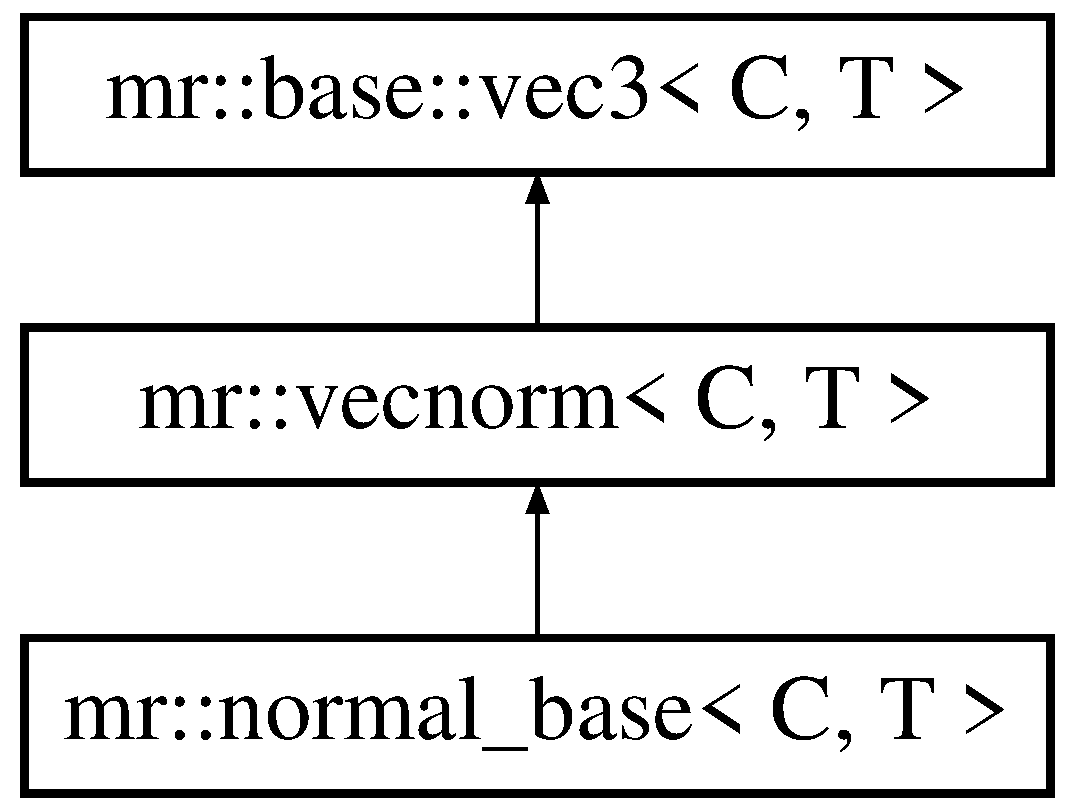
\includegraphics[height=3cm]{structmr_1_1normal__base}
\end{center}
\end{figure}
\subsection*{Public Types}
\begin{CompactItemize}
\item 
typedef {\bf normal\_\-base}$<$ C, T $>$ {\bf self}
\end{CompactItemize}
\subsection*{Public Member Functions}
\begin{CompactItemize}
\item 
void {\bf to\-Tangent} (const mi\-State $\ast$const state, const int idx=0)
\item 
void {\bf to\-Object} (const mi\-State $\ast$const state)
\item 
void {\bf to\-World} (const mi\-State $\ast$const state)
\item 
void {\bf to\-Camera} (const mi\-State $\ast$const state)
\item 
void {\bf to\-Raster} (const mi\-State $\ast$const state)
\item 
void {\bf to\-NDC} (const mi\-State $\ast$const state)
\item 
void {\bf to\-Light} (const mi\-State $\ast$const state)
\item 
void {\bf from\-Tangent} (const mi\-State $\ast$const state, const int idx=0)
\item 
void {\bf from\-Object} (const mi\-State $\ast$const state)
\item 
void {\bf from\-World} (const mi\-State $\ast$const state)
\item 
void {\bf from\-Camera} (const mi\-State $\ast$const state)
\item 
void {\bf from\-Light} (const mi\-State $\ast$const state)
\item 
void {\bf to} (const mi\-State $\ast$const state, const {\bf space::type} to\-Space)
\item 
void {\bf from} (const mi\-State $\ast$const state, const {\bf space::type} from\-Space)
\item 
void {\bf transform} (const mi\-State $\ast$const state, const {\bf space::type} from\-Space, const {\bf space::type} to\-Space)
\item 
{\bf self} {\bf inverse} () const 
\item 
{\bf self} {\bf operator-} () const 
\item 
{\bf self} {\bf normalized} () const 
\item 
{\bf self} {\bf normalized\-Fast} () const 
\item 
{\bf self} {\bf operator $\ast$} (const mi\-Matrix m) const 
\item 
{\bf self} {\bf operator $\ast$} (const {\bf matrix} \&m) const 
\end{CompactItemize}
\begin{Indent}{\bf Constructors}\par
\begin{CompactItemize}
\item 
{\bf normal\_\-base} ({\bf k\-No\-Construct})
\item 
{\bf normal\_\-base} ()
\item 
{\bf normal\_\-base} (const C \&b)
\item 
{\bf normal\_\-base} (const T b)
\item 
template$<$class X, class Y, class Oper$>$ {\bf normal\_\-base} (const {\bf base::exp}$<$ X, Y, Oper $>$ \&e)
\item 
{\bf normal\_\-base} (const T xx, const T yy=0.0f, const T zz=0.0f)
\item 
{\bf normal\_\-base} (const mi\-State $\ast$const state, const {\bf space::type} from\-Space, const T xx, const T yy, const T zz)
\item 
{\bf normal\_\-base} (const mi\-State $\ast$const state, const {\bf space::type} from\-Space, const C \&v)
\end{CompactItemize}
\end{Indent}
\begin{Indent}{\bf Copy Constructor}\par
\begin{CompactItemize}
\item 
{\bf normal\_\-base} (const {\bf self} \&b)
\end{CompactItemize}
\end{Indent}
\begin{Indent}{\bf Assignment}\par
\begin{CompactItemize}
\item 
template$<$class X, class Y, class Oper$>$ const {\bf self} \& {\bf operator=} (const {\bf base::exp}$<$ X, Y, Oper $>$ \&e)
\begin{CompactList}\small\item\em Handle assignment when we deal with a chained operation. \item\end{CompactList}\item 
const {\bf self} \& {\bf operator=} (const {\bf self} \&b)
\begin{CompactList}\small\item\em Assignment of similar object. \item\end{CompactList}\item 
const {\bf self} \& {\bf operator=} (const C \&b)
\begin{CompactList}\small\item\em Assignemnt of base class object. \item\end{CompactList}\item 
const {\bf self} \& {\bf operator=} (const T b)
\begin{CompactList}\small\item\em Assignment of base type. \item\end{CompactList}\end{CompactItemize}
\end{Indent}
\begin{Indent}{\bf REFERENCE OPERATORS (MODIFY IN PLACE)}\par
\begin{CompactItemize}
\item 
const {\bf self} \& {\bf operator $\ast$=} (const T b)
\item 
const {\bf self} \& {\bf operator $\ast$=} (const C \&b)
\item 
const {\bf self} \& {\bf operator $\ast$=} (const mi\-Matrix a)
\item 
const {\bf self} \& {\bf operator $\ast$=} (const {\bf matrix} \&m)
\end{CompactItemize}
\end{Indent}
\begin{Indent}{\bf Cross product}\par
\begin{CompactItemize}
\item 
template$<$class X, class Y, class Oper$>$ const {\bf self} \& {\bf operator$^\wedge$=} (const {\bf base::exp}$<$ X, Y, Oper $>$ \&b)
\item 
const {\bf self} \& {\bf operator$^\wedge$=} (const mi\-Vector \&b)
\item 
template$<$typename X$>$ const {\bf self} \& {\bf cross} (const X \&b)
\item 
template$<$class X, class Y, class Oper$>$ {\bf self} {\bf operator$^\wedge$} (const {\bf base::exp}$<$ X, Y, Oper $>$ \&b) const 
\item 
{\bf self} {\bf operator$^\wedge$} (const mi\-Vector \&b) const 
\end{CompactItemize}
\end{Indent}
\subsubsection*{template$<$class C, typename T$>$ struct mr::normal\_\-base$<$ C, T $>$}



\subsection{Member Typedef Documentation}
\index{mr::normal_base@{mr::normal\_\-base}!self@{self}}
\index{self@{self}!mr::normal_base@{mr::normal\_\-base}}
\subsubsection{\setlength{\rightskip}{0pt plus 5cm}template$<$class C, typename T$>$ typedef {\bf normal\_\-base}$<$ C, T $>$ {\bf mr::normal\_\-base}$<$ C, T $>$::{\bf self}}\label{structmr_1_1normal__base_w0}




Reimplemented from {\bf mr::vecnorm$<$ C, T $>$} {\rm (p.\,\pageref{structmr_1_1vecnorm_w0})}.

\subsection{Constructor \& Destructor Documentation}
\index{mr::normal_base@{mr::normal\_\-base}!normal_base@{normal\_\-base}}
\index{normal_base@{normal\_\-base}!mr::normal_base@{mr::normal\_\-base}}
\subsubsection{\setlength{\rightskip}{0pt plus 5cm}template$<$class C, typename T$>$ {\bf mr::normal\_\-base}$<$ C, T $>$::{\bf normal\_\-base} ({\bf k\-No\-Construct})\hspace{0.3cm}{\tt  [inline]}}\label{structmr_1_1normal__base_z66_0}


\index{mr::normal_base@{mr::normal\_\-base}!normal_base@{normal\_\-base}}
\index{normal_base@{normal\_\-base}!mr::normal_base@{mr::normal\_\-base}}
\subsubsection{\setlength{\rightskip}{0pt plus 5cm}template$<$class C, typename T$>$ {\bf mr::normal\_\-base}$<$ C, T $>$::{\bf normal\_\-base} ()\hspace{0.3cm}{\tt  [inline]}}\label{structmr_1_1normal__base_z66_1}


\index{mr::normal_base@{mr::normal\_\-base}!normal_base@{normal\_\-base}}
\index{normal_base@{normal\_\-base}!mr::normal_base@{mr::normal\_\-base}}
\subsubsection{\setlength{\rightskip}{0pt plus 5cm}template$<$class C, typename T$>$ {\bf mr::normal\_\-base}$<$ C, T $>$::{\bf normal\_\-base} (const C \& {\em b})\hspace{0.3cm}{\tt  [inline]}}\label{structmr_1_1normal__base_z66_2}


\index{mr::normal_base@{mr::normal\_\-base}!normal_base@{normal\_\-base}}
\index{normal_base@{normal\_\-base}!mr::normal_base@{mr::normal\_\-base}}
\subsubsection{\setlength{\rightskip}{0pt plus 5cm}template$<$class C, typename T$>$ {\bf mr::normal\_\-base}$<$ C, T $>$::{\bf normal\_\-base} (const T {\em b})\hspace{0.3cm}{\tt  [inline]}}\label{structmr_1_1normal__base_z66_3}


\index{mr::normal_base@{mr::normal\_\-base}!normal_base@{normal\_\-base}}
\index{normal_base@{normal\_\-base}!mr::normal_base@{mr::normal\_\-base}}
\subsubsection{\setlength{\rightskip}{0pt plus 5cm}template$<$class C, typename T$>$ template$<$class X, class Y, class Oper$>$ {\bf mr::normal\_\-base}$<$ C, T $>$::{\bf normal\_\-base} (const {\bf base::exp}$<$ X, Y, Oper $>$ \& {\em e})\hspace{0.3cm}{\tt  [inline]}}\label{structmr_1_1normal__base_z66_4}


\index{mr::normal_base@{mr::normal\_\-base}!normal_base@{normal\_\-base}}
\index{normal_base@{normal\_\-base}!mr::normal_base@{mr::normal\_\-base}}
\subsubsection{\setlength{\rightskip}{0pt plus 5cm}template$<$class C, typename T$>$ {\bf mr::normal\_\-base}$<$ C, T $>$::{\bf normal\_\-base} (const T {\em xx}, const T {\em yy} = 0.0f, const T {\em zz} = 0.0f)\hspace{0.3cm}{\tt  [inline]}}\label{structmr_1_1normal__base_z66_5}


\index{mr::normal_base@{mr::normal\_\-base}!normal_base@{normal\_\-base}}
\index{normal_base@{normal\_\-base}!mr::normal_base@{mr::normal\_\-base}}
\subsubsection{\setlength{\rightskip}{0pt plus 5cm}template$<$class C, typename T$>$ {\bf mr::normal\_\-base}$<$ C, T $>$::{\bf normal\_\-base} (const mi\-State $\ast$const {\em state}, const {\bf space::type} {\em from\-Space}, const T {\em xx}, const T {\em yy}, const T {\em zz})\hspace{0.3cm}{\tt  [inline]}}\label{structmr_1_1normal__base_z66_6}


\index{mr::normal_base@{mr::normal\_\-base}!normal_base@{normal\_\-base}}
\index{normal_base@{normal\_\-base}!mr::normal_base@{mr::normal\_\-base}}
\subsubsection{\setlength{\rightskip}{0pt plus 5cm}template$<$class C, typename T$>$ {\bf mr::normal\_\-base}$<$ C, T $>$::{\bf normal\_\-base} (const mi\-State $\ast$const {\em state}, const {\bf space::type} {\em from\-Space}, const C \& {\em v})\hspace{0.3cm}{\tt  [inline]}}\label{structmr_1_1normal__base_z66_7}


\index{mr::normal_base@{mr::normal\_\-base}!normal_base@{normal\_\-base}}
\index{normal_base@{normal\_\-base}!mr::normal_base@{mr::normal\_\-base}}
\subsubsection{\setlength{\rightskip}{0pt plus 5cm}template$<$class C, typename T$>$ {\bf mr::normal\_\-base}$<$ C, T $>$::{\bf normal\_\-base} (const {\bf self} \& {\em b})\hspace{0.3cm}{\tt  [inline]}}\label{structmr_1_1normal__base_z67_0}




\subsection{Member Function Documentation}
\index{mr::normal_base@{mr::normal\_\-base}!cross@{cross}}
\index{cross@{cross}!mr::normal_base@{mr::normal\_\-base}}
\subsubsection{\setlength{\rightskip}{0pt plus 5cm}template$<$class C, typename T$>$ template$<$typename X$>$ const {\bf self}\& {\bf mr::normal\_\-base}$<$ C, T $>$::cross (const X \& {\em b})\hspace{0.3cm}{\tt  [inline]}}\label{structmr_1_1normal__base_z73_2}


\index{mr::normal_base@{mr::normal\_\-base}!from@{from}}
\index{from@{from}!mr::normal_base@{mr::normal\_\-base}}
\subsubsection{\setlength{\rightskip}{0pt plus 5cm}template$<$class C, typename T$>$ void {\bf mr::normal\_\-base}$<$ C, T $>$::from (const mi\-State $\ast$const {\em state}, const {\bf space::type} {\em from\-Space})\hspace{0.3cm}{\tt  [inline]}}\label{structmr_1_1normal__base_a13}


\index{mr::normal_base@{mr::normal\_\-base}!fromCamera@{fromCamera}}
\index{fromCamera@{fromCamera}!mr::normal_base@{mr::normal\_\-base}}
\subsubsection{\setlength{\rightskip}{0pt plus 5cm}template$<$class C, typename T$>$ void {\bf mr::normal\_\-base}$<$ C, T $>$::from\-Camera (const mi\-State $\ast$const {\em state})\hspace{0.3cm}{\tt  [inline]}}\label{structmr_1_1normal__base_a10}


\index{mr::normal_base@{mr::normal\_\-base}!fromLight@{fromLight}}
\index{fromLight@{fromLight}!mr::normal_base@{mr::normal\_\-base}}
\subsubsection{\setlength{\rightskip}{0pt plus 5cm}template$<$class C, typename T$>$ void {\bf mr::normal\_\-base}$<$ C, T $>$::from\-Light (const mi\-State $\ast$const {\em state})\hspace{0.3cm}{\tt  [inline]}}\label{structmr_1_1normal__base_a11}


\index{mr::normal_base@{mr::normal\_\-base}!fromObject@{fromObject}}
\index{fromObject@{fromObject}!mr::normal_base@{mr::normal\_\-base}}
\subsubsection{\setlength{\rightskip}{0pt plus 5cm}template$<$class C, typename T$>$ void {\bf mr::normal\_\-base}$<$ C, T $>$::from\-Object (const mi\-State $\ast$const {\em state})\hspace{0.3cm}{\tt  [inline]}}\label{structmr_1_1normal__base_a8}


\index{mr::normal_base@{mr::normal\_\-base}!fromTangent@{fromTangent}}
\index{fromTangent@{fromTangent}!mr::normal_base@{mr::normal\_\-base}}
\subsubsection{\setlength{\rightskip}{0pt plus 5cm}template$<$class C, typename T$>$ void {\bf mr::normal\_\-base}$<$ C, T $>$::from\-Tangent (const mi\-State $\ast$const {\em state}, const int {\em idx} = 0)\hspace{0.3cm}{\tt  [inline]}}\label{structmr_1_1normal__base_a7}


\index{mr::normal_base@{mr::normal\_\-base}!fromWorld@{fromWorld}}
\index{fromWorld@{fromWorld}!mr::normal_base@{mr::normal\_\-base}}
\subsubsection{\setlength{\rightskip}{0pt plus 5cm}template$<$class C, typename T$>$ void {\bf mr::normal\_\-base}$<$ C, T $>$::from\-World (const mi\-State $\ast$const {\em state})\hspace{0.3cm}{\tt  [inline]}}\label{structmr_1_1normal__base_a9}


\index{mr::normal_base@{mr::normal\_\-base}!inverse@{inverse}}
\index{inverse@{inverse}!mr::normal_base@{mr::normal\_\-base}}
\subsubsection{\setlength{\rightskip}{0pt plus 5cm}template$<$class C, typename T$>$ {\bf self} {\bf mr::normal\_\-base}$<$ C, T $>$::inverse () const\hspace{0.3cm}{\tt  [inline]}}\label{structmr_1_1normal__base_a15}


\index{mr::normal_base@{mr::normal\_\-base}!normalized@{normalized}}
\index{normalized@{normalized}!mr::normal_base@{mr::normal\_\-base}}
\subsubsection{\setlength{\rightskip}{0pt plus 5cm}template$<$class C, typename T$>$ {\bf self} {\bf mr::normal\_\-base}$<$ C, T $>$::normalized () const\hspace{0.3cm}{\tt  [inline]}}\label{structmr_1_1normal__base_a17}


\index{mr::normal_base@{mr::normal\_\-base}!normalizedFast@{normalizedFast}}
\index{normalizedFast@{normalizedFast}!mr::normal_base@{mr::normal\_\-base}}
\subsubsection{\setlength{\rightskip}{0pt plus 5cm}template$<$class C, typename T$>$ {\bf self} {\bf mr::normal\_\-base}$<$ C, T $>$::normalized\-Fast () const\hspace{0.3cm}{\tt  [inline]}}\label{structmr_1_1normal__base_a18}


\index{mr::normal_base@{mr::normal\_\-base}!operator *@{operator $\ast$}}
\index{operator *@{operator $\ast$}!mr::normal_base@{mr::normal\_\-base}}
\subsubsection{\setlength{\rightskip}{0pt plus 5cm}template$<$class C, typename T$>$ {\bf self} {\bf mr::normal\_\-base}$<$ C, T $>$::operator $\ast$ (const {\bf matrix} \& {\em m}) const\hspace{0.3cm}{\tt  [inline]}}\label{structmr_1_1normal__base_a20}


\index{mr::normal_base@{mr::normal\_\-base}!operator *@{operator $\ast$}}
\index{operator *@{operator $\ast$}!mr::normal_base@{mr::normal\_\-base}}
\subsubsection{\setlength{\rightskip}{0pt plus 5cm}template$<$class C, typename T$>$ {\bf self} {\bf mr::normal\_\-base}$<$ C, T $>$::operator $\ast$ (const mi\-Matrix {\em m}) const\hspace{0.3cm}{\tt  [inline]}}\label{structmr_1_1normal__base_a19}


\index{mr::normal_base@{mr::normal\_\-base}!operator *=@{operator $\ast$=}}
\index{operator *=@{operator $\ast$=}!mr::normal_base@{mr::normal\_\-base}}
\subsubsection{\setlength{\rightskip}{0pt plus 5cm}template$<$class C, typename T$>$ const {\bf self}\& {\bf mr::normal\_\-base}$<$ C, T $>$::operator $\ast$= (const {\bf matrix} \& {\em m})\hspace{0.3cm}{\tt  [inline]}}\label{structmr_1_1normal__base_z71_3}


\index{mr::normal_base@{mr::normal\_\-base}!operator *=@{operator $\ast$=}}
\index{operator *=@{operator $\ast$=}!mr::normal_base@{mr::normal\_\-base}}
\subsubsection{\setlength{\rightskip}{0pt plus 5cm}template$<$class C, typename T$>$ const {\bf self}\& {\bf mr::normal\_\-base}$<$ C, T $>$::operator $\ast$= (const mi\-Matrix {\em a})\hspace{0.3cm}{\tt  [inline]}}\label{structmr_1_1normal__base_z71_2}


\index{mr::normal_base@{mr::normal\_\-base}!operator *=@{operator $\ast$=}}
\index{operator *=@{operator $\ast$=}!mr::normal_base@{mr::normal\_\-base}}
\subsubsection{\setlength{\rightskip}{0pt plus 5cm}template$<$class C, typename T$>$ const {\bf self}\& {\bf mr::normal\_\-base}$<$ C, T $>$::operator $\ast$= (const C \& {\em b})\hspace{0.3cm}{\tt  [inline]}}\label{structmr_1_1normal__base_z71_1}




Reimplemented from {\bf mr::base::vec3$<$ C, T $>$} {\rm (p.\,\pageref{structmr_1_1base_1_1vec3_z40_8})}.\index{mr::normal_base@{mr::normal\_\-base}!operator *=@{operator $\ast$=}}
\index{operator *=@{operator $\ast$=}!mr::normal_base@{mr::normal\_\-base}}
\subsubsection{\setlength{\rightskip}{0pt plus 5cm}template$<$class C, typename T$>$ const {\bf self}\& {\bf mr::normal\_\-base}$<$ C, T $>$::operator $\ast$= (const T {\em b})\hspace{0.3cm}{\tt  [inline]}}\label{structmr_1_1normal__base_z71_0}




Reimplemented from {\bf mr::base::vec3$<$ C, T $>$} {\rm (p.\,\pageref{structmr_1_1base_1_1vec3_z40_7})}.\index{mr::normal_base@{mr::normal\_\-base}!operator-@{operator-}}
\index{operator-@{operator-}!mr::normal_base@{mr::normal\_\-base}}
\subsubsection{\setlength{\rightskip}{0pt plus 5cm}template$<$class C, typename T$>$ {\bf self} {\bf mr::normal\_\-base}$<$ C, T $>$::operator- () const\hspace{0.3cm}{\tt  [inline]}}\label{structmr_1_1normal__base_a16}


\index{mr::normal_base@{mr::normal\_\-base}!operator=@{operator=}}
\index{operator=@{operator=}!mr::normal_base@{mr::normal\_\-base}}
\subsubsection{\setlength{\rightskip}{0pt plus 5cm}template$<$class C, typename T$>$ const {\bf self}\& {\bf mr::normal\_\-base}$<$ C, T $>$::operator= (const T {\em b})\hspace{0.3cm}{\tt  [inline]}}\label{structmr_1_1normal__base_z69_3}


Assignment of base type. 



Reimplemented from {\bf mr::base::vec3$<$ C, T $>$} {\rm (p.\,\pageref{structmr_1_1base_1_1vec3_z36_3})}.\index{mr::normal_base@{mr::normal\_\-base}!operator=@{operator=}}
\index{operator=@{operator=}!mr::normal_base@{mr::normal\_\-base}}
\subsubsection{\setlength{\rightskip}{0pt plus 5cm}template$<$class C, typename T$>$ const {\bf self}\& {\bf mr::normal\_\-base}$<$ C, T $>$::operator= (const C \& {\em b})\hspace{0.3cm}{\tt  [inline]}}\label{structmr_1_1normal__base_z69_2}


Assignemnt of base class object. 



Reimplemented from {\bf mr::base::vec3$<$ C, T $>$} {\rm (p.\,\pageref{structmr_1_1base_1_1vec3_z36_2})}.\index{mr::normal_base@{mr::normal\_\-base}!operator=@{operator=}}
\index{operator=@{operator=}!mr::normal_base@{mr::normal\_\-base}}
\subsubsection{\setlength{\rightskip}{0pt plus 5cm}template$<$class C, typename T$>$ const {\bf self}\& {\bf mr::normal\_\-base}$<$ C, T $>$::operator= (const {\bf self} \& {\em b})\hspace{0.3cm}{\tt  [inline]}}\label{structmr_1_1normal__base_z69_1}


Assignment of similar object. 



Reimplemented from {\bf mr::base::vec3$<$ C, T $>$} {\rm (p.\,\pageref{structmr_1_1base_1_1vec3_z36_1})}.\index{mr::normal_base@{mr::normal\_\-base}!operator=@{operator=}}
\index{operator=@{operator=}!mr::normal_base@{mr::normal\_\-base}}
\subsubsection{\setlength{\rightskip}{0pt plus 5cm}template$<$class C, typename T$>$ template$<$class X, class Y, class Oper$>$ const {\bf self}\& {\bf mr::normal\_\-base}$<$ C, T $>$::operator= (const {\bf base::exp}$<$ X, Y, Oper $>$ \& {\em e})\hspace{0.3cm}{\tt  [inline]}}\label{structmr_1_1normal__base_z69_0}


Handle assignment when we deal with a chained operation. 



Reimplemented from {\bf mr::base::vec3$<$ C, T $>$} {\rm (p.\,\pageref{structmr_1_1base_1_1vec3_z36_0})}.\index{mr::normal_base@{mr::normal\_\-base}!operator^@{operator$^\wedge$}}
\index{operator^@{operator$^\wedge$}!mr::normal_base@{mr::normal\_\-base}}
\subsubsection{\setlength{\rightskip}{0pt plus 5cm}template$<$class C, typename T$>$ {\bf self} {\bf mr::normal\_\-base}$<$ C, T $>$::operator$^\wedge$ (const mi\-Vector \& {\em b}) const\hspace{0.3cm}{\tt  [inline]}}\label{structmr_1_1normal__base_z73_4}


\index{mr::normal_base@{mr::normal\_\-base}!operator^@{operator$^\wedge$}}
\index{operator^@{operator$^\wedge$}!mr::normal_base@{mr::normal\_\-base}}
\subsubsection{\setlength{\rightskip}{0pt plus 5cm}template$<$class C, typename T$>$ template$<$class X, class Y, class Oper$>$ {\bf self} {\bf mr::normal\_\-base}$<$ C, T $>$::operator$^\wedge$ (const {\bf base::exp}$<$ X, Y, Oper $>$ \& {\em b}) const\hspace{0.3cm}{\tt  [inline]}}\label{structmr_1_1normal__base_z73_3}


\index{mr::normal_base@{mr::normal\_\-base}!operator^=@{operator$^\wedge$=}}
\index{operator^=@{operator$^\wedge$=}!mr::normal_base@{mr::normal\_\-base}}
\subsubsection{\setlength{\rightskip}{0pt plus 5cm}template$<$class C, typename T$>$ const {\bf self}\& {\bf mr::normal\_\-base}$<$ C, T $>$::operator$^\wedge$= (const mi\-Vector \& {\em b})\hspace{0.3cm}{\tt  [inline]}}\label{structmr_1_1normal__base_z73_1}


\index{mr::normal_base@{mr::normal\_\-base}!operator^=@{operator$^\wedge$=}}
\index{operator^=@{operator$^\wedge$=}!mr::normal_base@{mr::normal\_\-base}}
\subsubsection{\setlength{\rightskip}{0pt plus 5cm}template$<$class C, typename T$>$ template$<$class X, class Y, class Oper$>$ const {\bf self}\& {\bf mr::normal\_\-base}$<$ C, T $>$::operator$^\wedge$= (const {\bf base::exp}$<$ X, Y, Oper $>$ \& {\em b})\hspace{0.3cm}{\tt  [inline]}}\label{structmr_1_1normal__base_z73_0}


\index{mr::normal_base@{mr::normal\_\-base}!to@{to}}
\index{to@{to}!mr::normal_base@{mr::normal\_\-base}}
\subsubsection{\setlength{\rightskip}{0pt plus 5cm}template$<$class C, typename T$>$ void {\bf mr::normal\_\-base}$<$ C, T $>$::to (const mi\-State $\ast$const {\em state}, const {\bf space::type} {\em to\-Space})\hspace{0.3cm}{\tt  [inline]}}\label{structmr_1_1normal__base_a12}


\index{mr::normal_base@{mr::normal\_\-base}!toCamera@{toCamera}}
\index{toCamera@{toCamera}!mr::normal_base@{mr::normal\_\-base}}
\subsubsection{\setlength{\rightskip}{0pt plus 5cm}template$<$class C, typename T$>$ void {\bf mr::normal\_\-base}$<$ C, T $>$::to\-Camera (const mi\-State $\ast$const {\em state})\hspace{0.3cm}{\tt  [inline]}}\label{structmr_1_1normal__base_a3}


\index{mr::normal_base@{mr::normal\_\-base}!toLight@{toLight}}
\index{toLight@{toLight}!mr::normal_base@{mr::normal\_\-base}}
\subsubsection{\setlength{\rightskip}{0pt plus 5cm}template$<$class C, typename T$>$ void {\bf mr::normal\_\-base}$<$ C, T $>$::to\-Light (const mi\-State $\ast$const {\em state})\hspace{0.3cm}{\tt  [inline]}}\label{structmr_1_1normal__base_a6}


\index{mr::normal_base@{mr::normal\_\-base}!toNDC@{toNDC}}
\index{toNDC@{toNDC}!mr::normal_base@{mr::normal\_\-base}}
\subsubsection{\setlength{\rightskip}{0pt plus 5cm}template$<$class C, typename T$>$ void {\bf mr::normal\_\-base}$<$ C, T $>$::to\-NDC (const mi\-State $\ast$const {\em state})\hspace{0.3cm}{\tt  [inline]}}\label{structmr_1_1normal__base_a5}


\index{mr::normal_base@{mr::normal\_\-base}!toObject@{toObject}}
\index{toObject@{toObject}!mr::normal_base@{mr::normal\_\-base}}
\subsubsection{\setlength{\rightskip}{0pt plus 5cm}template$<$class C, typename T$>$ void {\bf mr::normal\_\-base}$<$ C, T $>$::to\-Object (const mi\-State $\ast$const {\em state})\hspace{0.3cm}{\tt  [inline]}}\label{structmr_1_1normal__base_a1}


\index{mr::normal_base@{mr::normal\_\-base}!toRaster@{toRaster}}
\index{toRaster@{toRaster}!mr::normal_base@{mr::normal\_\-base}}
\subsubsection{\setlength{\rightskip}{0pt plus 5cm}template$<$class C, typename T$>$ void {\bf mr::normal\_\-base}$<$ C, T $>$::to\-Raster (const mi\-State $\ast$const {\em state})\hspace{0.3cm}{\tt  [inline]}}\label{structmr_1_1normal__base_a4}


\index{mr::normal_base@{mr::normal\_\-base}!toTangent@{toTangent}}
\index{toTangent@{toTangent}!mr::normal_base@{mr::normal\_\-base}}
\subsubsection{\setlength{\rightskip}{0pt plus 5cm}template$<$class C, typename T$>$ void {\bf mr::normal\_\-base}$<$ C, T $>$::to\-Tangent (const mi\-State $\ast$const {\em state}, const int {\em idx} = 0)\hspace{0.3cm}{\tt  [inline]}}\label{structmr_1_1normal__base_a0}


\index{mr::normal_base@{mr::normal\_\-base}!toWorld@{toWorld}}
\index{toWorld@{toWorld}!mr::normal_base@{mr::normal\_\-base}}
\subsubsection{\setlength{\rightskip}{0pt plus 5cm}template$<$class C, typename T$>$ void {\bf mr::normal\_\-base}$<$ C, T $>$::to\-World (const mi\-State $\ast$const {\em state})\hspace{0.3cm}{\tt  [inline]}}\label{structmr_1_1normal__base_a2}


\index{mr::normal_base@{mr::normal\_\-base}!transform@{transform}}
\index{transform@{transform}!mr::normal_base@{mr::normal\_\-base}}
\subsubsection{\setlength{\rightskip}{0pt plus 5cm}template$<$class C, typename T$>$ void {\bf mr::normal\_\-base}$<$ C, T $>$::transform (const mi\-State $\ast$const {\em state}, const {\bf space::type} {\em from\-Space}, const {\bf space::type} {\em to\-Space})\hspace{0.3cm}{\tt  [inline]}}\label{structmr_1_1normal__base_a14}




The documentation for this struct was generated from the following files:\begin{CompactItemize}
\item 
{\bf mr\-Vector.h}\item 
{\bf mr\-Derivs.h}\end{CompactItemize}

\section{mr::point\_\-base$<$ C, T $>$ Struct Template Reference}
\label{structmr_1_1point__base}\index{mr::point_base@{mr::point\_\-base}}
{\tt \#include $<$mr\-Vector.h$>$}

Inheritance diagram for mr::point\_\-base$<$ C, T $>$::\begin{figure}[H]
\begin{center}
\leavevmode
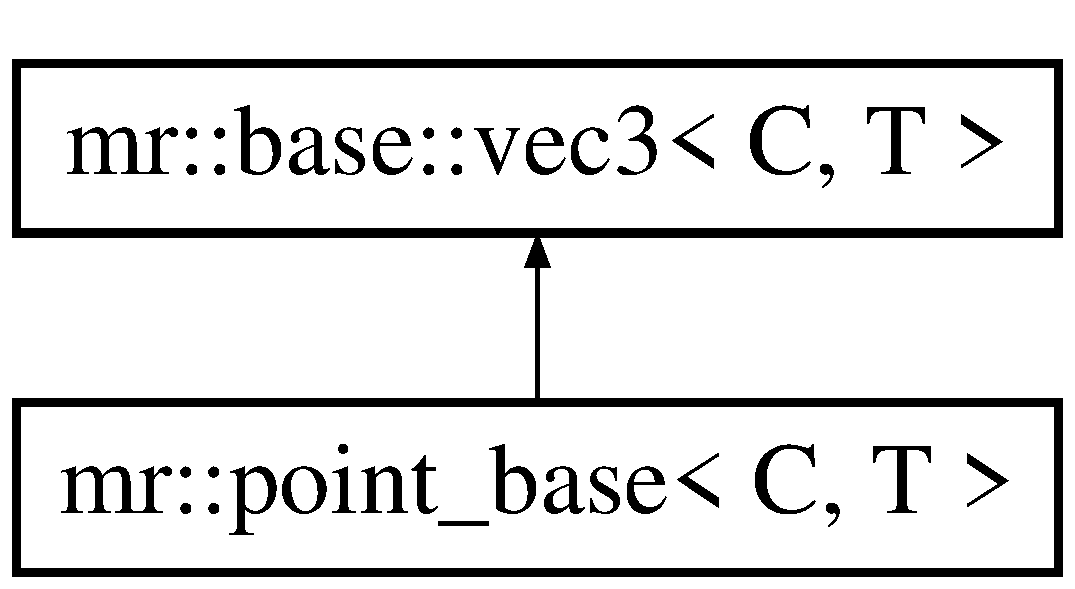
\includegraphics[height=2cm]{structmr_1_1point__base}
\end{center}
\end{figure}
\subsection*{Public Types}
\begin{CompactItemize}
\item 
typedef {\bf point\_\-base}$<$ C, T $>$ {\bf self}
\end{CompactItemize}
\subsection*{Public Member Functions}
\begin{Indent}{\bf Space Conversions}\par
\begin{CompactItemize}
\item 
void {\bf to\-Object} (const mi\-State $\ast$const state)
\item 
void {\bf to\-World} (const mi\-State $\ast$const state)
\item 
void {\bf to\-Camera} (const mi\-State $\ast$const state)
\item 
void {\bf to\-Screen} (const mi\-State $\ast$const state)
\item 
void {\bf to\-NDC} (const mi\-State $\ast$const state)
\item 
void {\bf to\-Raster} (const mi\-State $\ast$const state)
\item 
void {\bf to\-Light} (const mi\-State $\ast$const state)
\item 
void {\bf from\-Object} (const mi\-State $\ast$const state)
\item 
void {\bf from\-World} (const mi\-State $\ast$const state)
\item 
void {\bf from\-Camera} (const mi\-State $\ast$const state)
\item 
void {\bf from\-Screen} (const mi\-State $\ast$const state)
\item 
void {\bf from\-NDC} (const mi\-State $\ast$const state)
\item 
void {\bf from\-Raster} (const mi\-State $\ast$const state)
\item 
void {\bf from\-Light} (const mi\-State $\ast$const state)
\item 
void {\bf to} (const mi\-State $\ast$const state, const {\bf space::type} to\-Space)
\item 
void {\bf from} (const mi\-State $\ast$const state, const {\bf space::type} from\-Space)
\item 
void {\bf transform} (const mi\-State $\ast$const state, const {\bf space::type} from\-Space, const {\bf space::type} to\-Space)
\end{CompactItemize}
\end{Indent}
\begin{Indent}{\bf Constructors}\par
\begin{CompactItemize}
\item 
{\bf point\_\-base} ()
\begin{CompactList}\small\item\em Default constructor. \item\end{CompactList}\item 
{\bf point\_\-base} (const T xx, const T yy=0.0f, const T zz=0.0f)
\begin{CompactList}\small\item\em Multielement constructors. \item\end{CompactList}\item 
{\bf point\_\-base} (const mi\-State $\ast$const state, const {\bf space::type} to\-Space, const T xx, const T yy, const T zz)
\item 
{\bf point\_\-base} (const mi\-State $\ast$const state, const {\bf space::type} from\-Space, const C \&v)
\item 
template$<$class X, class Y, class Oper$>$ {\bf point\_\-base} (const {\bf base::exp}$<$ X, Y, Oper $>$ \&e)
\begin{CompactList}\small\item\em Single element constructors. \item\end{CompactList}\item 
{\bf point\_\-base} ({\bf k\-No\-Construct})
\item 
{\bf point\_\-base} (const C \&b)
\item 
{\bf point\_\-base} (const T b)
\end{CompactItemize}
\end{Indent}
\begin{Indent}{\bf Copy constructor}\par
\begin{CompactItemize}
\item 
{\bf point\_\-base} (const {\bf self} \&b)
\end{CompactItemize}
\end{Indent}
\begin{Indent}{\bf Assignment}\par
\begin{CompactItemize}
\item 
template$<$class X, class Y, class Oper$>$ const {\bf self} \& {\bf operator=} (const {\bf base::exp}$<$ X, Y, Oper $>$ \&e)
\begin{CompactList}\small\item\em Handle assignment when we deal with a chained operation. \item\end{CompactList}\item 
const {\bf self} \& {\bf operator=} (const {\bf self} \&b)
\begin{CompactList}\small\item\em Assignment of similar object. \item\end{CompactList}\item 
const {\bf self} \& {\bf operator=} (const C \&b)
\begin{CompactList}\small\item\em Assignemnt of base class object. \item\end{CompactList}\item 
const {\bf self} \& {\bf operator=} (const T b)
\begin{CompactList}\small\item\em Assignment of base type. \item\end{CompactList}\end{CompactItemize}
\end{Indent}
\begin{Indent}{\bf REFERENCE OPERATORS (MODIFY IN PLACE)}\par
\begin{CompactItemize}
\item 
const {\bf self} \& {\bf operator $\ast$=} (const T b)
\item 
const {\bf self} \& {\bf operator $\ast$=} (const C \&b)
\item 
const {\bf self} \& {\bf operator $\ast$=} (const mi\-Matrix a)
\item 
{\bf self} {\bf operator $\ast$} (const mi\-Matrix m) const 
\begin{CompactList}\small\item\em Matrix post-multiplication. \item\end{CompactList}\item 
const {\bf self} \& {\bf operator $\ast$=} (const {\bf matrix} \&m)
\begin{CompactList}\small\item\em In-place matrix post-multiplication. \item\end{CompactList}\item 
{\bf self} {\bf operator $\ast$} (const {\bf matrix} \&m) const 
\begin{CompactList}\small\item\em Matrix post-multiplication. \item\end{CompactList}\end{CompactItemize}
\end{Indent}
\subsection*{Static Public Attributes}
\begin{CompactItemize}
\item 
{\bf point\_\-base}$<$ C, T $>$ {\bf k\-Origin}
\end{CompactItemize}
\subsubsection*{template$<$class C, typename T$>$ struct mr::point\_\-base$<$ C, T $>$}



\subsection{Member Typedef Documentation}
\index{mr::point_base@{mr::point\_\-base}!self@{self}}
\index{self@{self}!mr::point_base@{mr::point\_\-base}}
\subsubsection{\setlength{\rightskip}{0pt plus 5cm}template$<$class C, typename T$>$ typedef {\bf point\_\-base}$<$ C, T $>$ {\bf mr::point\_\-base}$<$ C, T $>$::{\bf self}}\label{structmr_1_1point__base_w0}




Reimplemented from {\bf mr::base::vec3$<$ C, T $>$} {\rm (p.\,\pageref{structmr_1_1base_1_1vec3_w0})}.

\subsection{Constructor \& Destructor Documentation}
\index{mr::point_base@{mr::point\_\-base}!point_base@{point\_\-base}}
\index{point_base@{point\_\-base}!mr::point_base@{mr::point\_\-base}}
\subsubsection{\setlength{\rightskip}{0pt plus 5cm}template$<$class C, typename T$>$ {\bf mr::point\_\-base}$<$ C, T $>$::{\bf point\_\-base} ()\hspace{0.3cm}{\tt  [inline]}}\label{structmr_1_1point__base_z75_0}


Default constructor. 

\index{mr::point_base@{mr::point\_\-base}!point_base@{point\_\-base}}
\index{point_base@{point\_\-base}!mr::point_base@{mr::point\_\-base}}
\subsubsection{\setlength{\rightskip}{0pt plus 5cm}template$<$class C, typename T$>$ {\bf mr::point\_\-base}$<$ C, T $>$::{\bf point\_\-base} (const T {\em xx}, const T {\em yy} = 0.0f, const T {\em zz} = 0.0f)\hspace{0.3cm}{\tt  [inline]}}\label{structmr_1_1point__base_z75_1}


Multielement constructors. 

\index{mr::point_base@{mr::point\_\-base}!point_base@{point\_\-base}}
\index{point_base@{point\_\-base}!mr::point_base@{mr::point\_\-base}}
\subsubsection{\setlength{\rightskip}{0pt plus 5cm}template$<$class C, typename T$>$ {\bf mr::point\_\-base}$<$ C, T $>$::{\bf point\_\-base} (const mi\-State $\ast$const {\em state}, const {\bf space::type} {\em to\-Space}, const T {\em xx}, const T {\em yy}, const T {\em zz})\hspace{0.3cm}{\tt  [inline]}}\label{structmr_1_1point__base_z75_2}


\index{mr::point_base@{mr::point\_\-base}!point_base@{point\_\-base}}
\index{point_base@{point\_\-base}!mr::point_base@{mr::point\_\-base}}
\subsubsection{\setlength{\rightskip}{0pt plus 5cm}template$<$class C, typename T$>$ {\bf mr::point\_\-base}$<$ C, T $>$::{\bf point\_\-base} (const mi\-State $\ast$const {\em state}, const {\bf space::type} {\em from\-Space}, const C \& {\em v})\hspace{0.3cm}{\tt  [inline]}}\label{structmr_1_1point__base_z75_3}


\index{mr::point_base@{mr::point\_\-base}!point_base@{point\_\-base}}
\index{point_base@{point\_\-base}!mr::point_base@{mr::point\_\-base}}
\subsubsection{\setlength{\rightskip}{0pt plus 5cm}template$<$class C, typename T$>$ template$<$class X, class Y, class Oper$>$ {\bf mr::point\_\-base}$<$ C, T $>$::{\bf point\_\-base} (const {\bf base::exp}$<$ X, Y, Oper $>$ \& {\em e})\hspace{0.3cm}{\tt  [inline]}}\label{structmr_1_1point__base_z75_4}


Single element constructors. 

\index{mr::point_base@{mr::point\_\-base}!point_base@{point\_\-base}}
\index{point_base@{point\_\-base}!mr::point_base@{mr::point\_\-base}}
\subsubsection{\setlength{\rightskip}{0pt plus 5cm}template$<$class C, typename T$>$ {\bf mr::point\_\-base}$<$ C, T $>$::{\bf point\_\-base} ({\bf k\-No\-Construct})\hspace{0.3cm}{\tt  [inline]}}\label{structmr_1_1point__base_z75_5}


\index{mr::point_base@{mr::point\_\-base}!point_base@{point\_\-base}}
\index{point_base@{point\_\-base}!mr::point_base@{mr::point\_\-base}}
\subsubsection{\setlength{\rightskip}{0pt plus 5cm}template$<$class C, typename T$>$ {\bf mr::point\_\-base}$<$ C, T $>$::{\bf point\_\-base} (const C \& {\em b})\hspace{0.3cm}{\tt  [inline]}}\label{structmr_1_1point__base_z75_6}


\index{mr::point_base@{mr::point\_\-base}!point_base@{point\_\-base}}
\index{point_base@{point\_\-base}!mr::point_base@{mr::point\_\-base}}
\subsubsection{\setlength{\rightskip}{0pt plus 5cm}template$<$class C, typename T$>$ {\bf mr::point\_\-base}$<$ C, T $>$::{\bf point\_\-base} (const T {\em b})\hspace{0.3cm}{\tt  [inline]}}\label{structmr_1_1point__base_z75_7}


\index{mr::point_base@{mr::point\_\-base}!point_base@{point\_\-base}}
\index{point_base@{point\_\-base}!mr::point_base@{mr::point\_\-base}}
\subsubsection{\setlength{\rightskip}{0pt plus 5cm}template$<$class C, typename T$>$ {\bf mr::point\_\-base}$<$ C, T $>$::{\bf point\_\-base} (const {\bf self} \& {\em b})\hspace{0.3cm}{\tt  [inline]}}\label{structmr_1_1point__base_z76_0}




\subsection{Member Function Documentation}
\index{mr::point_base@{mr::point\_\-base}!from@{from}}
\index{from@{from}!mr::point_base@{mr::point\_\-base}}
\subsubsection{\setlength{\rightskip}{0pt plus 5cm}template$<$class C, typename T$>$ void {\bf mr::point\_\-base}$<$ C, T $>$::from (const mi\-State $\ast$const {\em state}, const {\bf space::type} {\em from\-Space})\hspace{0.3cm}{\tt  [inline]}}\label{structmr_1_1point__base_z74_15}


\index{mr::point_base@{mr::point\_\-base}!fromCamera@{fromCamera}}
\index{fromCamera@{fromCamera}!mr::point_base@{mr::point\_\-base}}
\subsubsection{\setlength{\rightskip}{0pt plus 5cm}template$<$class C, typename T$>$ void {\bf mr::point\_\-base}$<$ C, T $>$::from\-Camera (const mi\-State $\ast$const {\em state})\hspace{0.3cm}{\tt  [inline]}}\label{structmr_1_1point__base_z74_9}


\index{mr::point_base@{mr::point\_\-base}!fromLight@{fromLight}}
\index{fromLight@{fromLight}!mr::point_base@{mr::point\_\-base}}
\subsubsection{\setlength{\rightskip}{0pt plus 5cm}template$<$class C, typename T$>$ void {\bf mr::point\_\-base}$<$ C, T $>$::from\-Light (const mi\-State $\ast$const {\em state})\hspace{0.3cm}{\tt  [inline]}}\label{structmr_1_1point__base_z74_13}


\index{mr::point_base@{mr::point\_\-base}!fromNDC@{fromNDC}}
\index{fromNDC@{fromNDC}!mr::point_base@{mr::point\_\-base}}
\subsubsection{\setlength{\rightskip}{0pt plus 5cm}template$<$class C, typename T$>$ void {\bf mr::point\_\-base}$<$ C, T $>$::from\-NDC (const mi\-State $\ast$const {\em state})\hspace{0.3cm}{\tt  [inline]}}\label{structmr_1_1point__base_z74_11}


\index{mr::point_base@{mr::point\_\-base}!fromObject@{fromObject}}
\index{fromObject@{fromObject}!mr::point_base@{mr::point\_\-base}}
\subsubsection{\setlength{\rightskip}{0pt plus 5cm}template$<$class C, typename T$>$ void {\bf mr::point\_\-base}$<$ C, T $>$::from\-Object (const mi\-State $\ast$const {\em state})\hspace{0.3cm}{\tt  [inline]}}\label{structmr_1_1point__base_z74_7}


\index{mr::point_base@{mr::point\_\-base}!fromRaster@{fromRaster}}
\index{fromRaster@{fromRaster}!mr::point_base@{mr::point\_\-base}}
\subsubsection{\setlength{\rightskip}{0pt plus 5cm}template$<$class C, typename T$>$ void {\bf mr::point\_\-base}$<$ C, T $>$::from\-Raster (const mi\-State $\ast$const {\em state})\hspace{0.3cm}{\tt  [inline]}}\label{structmr_1_1point__base_z74_12}


\index{mr::point_base@{mr::point\_\-base}!fromScreen@{fromScreen}}
\index{fromScreen@{fromScreen}!mr::point_base@{mr::point\_\-base}}
\subsubsection{\setlength{\rightskip}{0pt plus 5cm}template$<$class C, typename T$>$ void {\bf mr::point\_\-base}$<$ C, T $>$::from\-Screen (const mi\-State $\ast$const {\em state})\hspace{0.3cm}{\tt  [inline]}}\label{structmr_1_1point__base_z74_10}


\index{mr::point_base@{mr::point\_\-base}!fromWorld@{fromWorld}}
\index{fromWorld@{fromWorld}!mr::point_base@{mr::point\_\-base}}
\subsubsection{\setlength{\rightskip}{0pt plus 5cm}template$<$class C, typename T$>$ void {\bf mr::point\_\-base}$<$ C, T $>$::from\-World (const mi\-State $\ast$const {\em state})\hspace{0.3cm}{\tt  [inline]}}\label{structmr_1_1point__base_z74_8}


\index{mr::point_base@{mr::point\_\-base}!operator *@{operator $\ast$}}
\index{operator *@{operator $\ast$}!mr::point_base@{mr::point\_\-base}}
\subsubsection{\setlength{\rightskip}{0pt plus 5cm}template$<$class C, typename T$>$ {\bf self} {\bf mr::point\_\-base}$<$ C, T $>$::operator $\ast$ (const {\bf matrix} \& {\em m}) const\hspace{0.3cm}{\tt  [inline]}}\label{structmr_1_1point__base_z78_5}


Matrix post-multiplication. 

\index{mr::point_base@{mr::point\_\-base}!operator *@{operator $\ast$}}
\index{operator *@{operator $\ast$}!mr::point_base@{mr::point\_\-base}}
\subsubsection{\setlength{\rightskip}{0pt plus 5cm}template$<$class C, typename T$>$ {\bf self} {\bf mr::point\_\-base}$<$ C, T $>$::operator $\ast$ (const mi\-Matrix {\em m}) const\hspace{0.3cm}{\tt  [inline]}}\label{structmr_1_1point__base_z78_3}


Matrix post-multiplication. 

\index{mr::point_base@{mr::point\_\-base}!operator *=@{operator $\ast$=}}
\index{operator *=@{operator $\ast$=}!mr::point_base@{mr::point\_\-base}}
\subsubsection{\setlength{\rightskip}{0pt plus 5cm}template$<$class C, typename T$>$ const {\bf self}\& {\bf mr::point\_\-base}$<$ C, T $>$::operator $\ast$= (const {\bf matrix} \& {\em m})\hspace{0.3cm}{\tt  [inline]}}\label{structmr_1_1point__base_z78_4}


In-place matrix post-multiplication. 

\index{mr::point_base@{mr::point\_\-base}!operator *=@{operator $\ast$=}}
\index{operator *=@{operator $\ast$=}!mr::point_base@{mr::point\_\-base}}
\subsubsection{\setlength{\rightskip}{0pt plus 5cm}template$<$class C, typename T$>$ const {\bf self}\& {\bf mr::point\_\-base}$<$ C, T $>$::operator $\ast$= (const mi\-Matrix {\em a})\hspace{0.3cm}{\tt  [inline]}}\label{structmr_1_1point__base_z78_2}


\index{mr::point_base@{mr::point\_\-base}!operator *=@{operator $\ast$=}}
\index{operator *=@{operator $\ast$=}!mr::point_base@{mr::point\_\-base}}
\subsubsection{\setlength{\rightskip}{0pt plus 5cm}template$<$class C, typename T$>$ const {\bf self}\& {\bf mr::point\_\-base}$<$ C, T $>$::operator $\ast$= (const C \& {\em b})\hspace{0.3cm}{\tt  [inline]}}\label{structmr_1_1point__base_z78_1}




Reimplemented from {\bf mr::base::vec3$<$ C, T $>$} {\rm (p.\,\pageref{structmr_1_1base_1_1vec3_z40_8})}.\index{mr::point_base@{mr::point\_\-base}!operator *=@{operator $\ast$=}}
\index{operator *=@{operator $\ast$=}!mr::point_base@{mr::point\_\-base}}
\subsubsection{\setlength{\rightskip}{0pt plus 5cm}template$<$class C, typename T$>$ const {\bf self}\& {\bf mr::point\_\-base}$<$ C, T $>$::operator $\ast$= (const T {\em b})\hspace{0.3cm}{\tt  [inline]}}\label{structmr_1_1point__base_z78_0}




Reimplemented from {\bf mr::base::vec3$<$ C, T $>$} {\rm (p.\,\pageref{structmr_1_1base_1_1vec3_z40_7})}.\index{mr::point_base@{mr::point\_\-base}!operator=@{operator=}}
\index{operator=@{operator=}!mr::point_base@{mr::point\_\-base}}
\subsubsection{\setlength{\rightskip}{0pt plus 5cm}template$<$class C, typename T$>$ const {\bf self}\& {\bf mr::point\_\-base}$<$ C, T $>$::operator= (const T {\em b})\hspace{0.3cm}{\tt  [inline]}}\label{structmr_1_1point__base_z77_3}


Assignment of base type. 



Reimplemented from {\bf mr::base::vec3$<$ C, T $>$} {\rm (p.\,\pageref{structmr_1_1base_1_1vec3_z36_3})}.\index{mr::point_base@{mr::point\_\-base}!operator=@{operator=}}
\index{operator=@{operator=}!mr::point_base@{mr::point\_\-base}}
\subsubsection{\setlength{\rightskip}{0pt plus 5cm}template$<$class C, typename T$>$ const {\bf self}\& {\bf mr::point\_\-base}$<$ C, T $>$::operator= (const C \& {\em b})\hspace{0.3cm}{\tt  [inline]}}\label{structmr_1_1point__base_z77_2}


Assignemnt of base class object. 



Reimplemented from {\bf mr::base::vec3$<$ C, T $>$} {\rm (p.\,\pageref{structmr_1_1base_1_1vec3_z36_2})}.\index{mr::point_base@{mr::point\_\-base}!operator=@{operator=}}
\index{operator=@{operator=}!mr::point_base@{mr::point\_\-base}}
\subsubsection{\setlength{\rightskip}{0pt plus 5cm}template$<$class C, typename T$>$ const {\bf self}\& {\bf mr::point\_\-base}$<$ C, T $>$::operator= (const {\bf self} \& {\em b})\hspace{0.3cm}{\tt  [inline]}}\label{structmr_1_1point__base_z77_1}


Assignment of similar object. 



Reimplemented from {\bf mr::base::vec3$<$ C, T $>$} {\rm (p.\,\pageref{structmr_1_1base_1_1vec3_z36_1})}.\index{mr::point_base@{mr::point\_\-base}!operator=@{operator=}}
\index{operator=@{operator=}!mr::point_base@{mr::point\_\-base}}
\subsubsection{\setlength{\rightskip}{0pt plus 5cm}template$<$class C, typename T$>$ template$<$class X, class Y, class Oper$>$ const {\bf self}\& {\bf mr::point\_\-base}$<$ C, T $>$::operator= (const {\bf base::exp}$<$ X, Y, Oper $>$ \& {\em e})\hspace{0.3cm}{\tt  [inline]}}\label{structmr_1_1point__base_z77_0}


Handle assignment when we deal with a chained operation. 



Reimplemented from {\bf mr::base::vec3$<$ C, T $>$} {\rm (p.\,\pageref{structmr_1_1base_1_1vec3_z36_0})}.\index{mr::point_base@{mr::point\_\-base}!to@{to}}
\index{to@{to}!mr::point_base@{mr::point\_\-base}}
\subsubsection{\setlength{\rightskip}{0pt plus 5cm}template$<$class C, typename T$>$ void {\bf mr::point\_\-base}$<$ C, T $>$::to (const mi\-State $\ast$const {\em state}, const {\bf space::type} {\em to\-Space})\hspace{0.3cm}{\tt  [inline]}}\label{structmr_1_1point__base_z74_14}


\index{mr::point_base@{mr::point\_\-base}!toCamera@{toCamera}}
\index{toCamera@{toCamera}!mr::point_base@{mr::point\_\-base}}
\subsubsection{\setlength{\rightskip}{0pt plus 5cm}template$<$class C, typename T$>$ void {\bf mr::point\_\-base}$<$ C, T $>$::to\-Camera (const mi\-State $\ast$const {\em state})\hspace{0.3cm}{\tt  [inline]}}\label{structmr_1_1point__base_z74_2}


\index{mr::point_base@{mr::point\_\-base}!toLight@{toLight}}
\index{toLight@{toLight}!mr::point_base@{mr::point\_\-base}}
\subsubsection{\setlength{\rightskip}{0pt plus 5cm}template$<$class C, typename T$>$ void {\bf mr::point\_\-base}$<$ C, T $>$::to\-Light (const mi\-State $\ast$const {\em state})\hspace{0.3cm}{\tt  [inline]}}\label{structmr_1_1point__base_z74_6}


\index{mr::point_base@{mr::point\_\-base}!toNDC@{toNDC}}
\index{toNDC@{toNDC}!mr::point_base@{mr::point\_\-base}}
\subsubsection{\setlength{\rightskip}{0pt plus 5cm}template$<$class C, typename T$>$ void {\bf mr::point\_\-base}$<$ C, T $>$::to\-NDC (const mi\-State $\ast$const {\em state})\hspace{0.3cm}{\tt  [inline]}}\label{structmr_1_1point__base_z74_4}


\index{mr::point_base@{mr::point\_\-base}!toObject@{toObject}}
\index{toObject@{toObject}!mr::point_base@{mr::point\_\-base}}
\subsubsection{\setlength{\rightskip}{0pt plus 5cm}template$<$class C, typename T$>$ void {\bf mr::point\_\-base}$<$ C, T $>$::to\-Object (const mi\-State $\ast$const {\em state})\hspace{0.3cm}{\tt  [inline]}}\label{structmr_1_1point__base_z74_0}


\index{mr::point_base@{mr::point\_\-base}!toRaster@{toRaster}}
\index{toRaster@{toRaster}!mr::point_base@{mr::point\_\-base}}
\subsubsection{\setlength{\rightskip}{0pt plus 5cm}template$<$class C, typename T$>$ void {\bf mr::point\_\-base}$<$ C, T $>$::to\-Raster (const mi\-State $\ast$const {\em state})\hspace{0.3cm}{\tt  [inline]}}\label{structmr_1_1point__base_z74_5}


\index{mr::point_base@{mr::point\_\-base}!toScreen@{toScreen}}
\index{toScreen@{toScreen}!mr::point_base@{mr::point\_\-base}}
\subsubsection{\setlength{\rightskip}{0pt plus 5cm}template$<$class C, typename T$>$ void {\bf mr::point\_\-base}$<$ C, T $>$::to\-Screen (const mi\-State $\ast$const {\em state})\hspace{0.3cm}{\tt  [inline]}}\label{structmr_1_1point__base_z74_3}


\index{mr::point_base@{mr::point\_\-base}!toWorld@{toWorld}}
\index{toWorld@{toWorld}!mr::point_base@{mr::point\_\-base}}
\subsubsection{\setlength{\rightskip}{0pt plus 5cm}template$<$class C, typename T$>$ void {\bf mr::point\_\-base}$<$ C, T $>$::to\-World (const mi\-State $\ast$const {\em state})\hspace{0.3cm}{\tt  [inline]}}\label{structmr_1_1point__base_z74_1}


\index{mr::point_base@{mr::point\_\-base}!transform@{transform}}
\index{transform@{transform}!mr::point_base@{mr::point\_\-base}}
\subsubsection{\setlength{\rightskip}{0pt plus 5cm}template$<$class C, typename T$>$ void {\bf mr::point\_\-base}$<$ C, T $>$::transform (const mi\-State $\ast$const {\em state}, const {\bf space::type} {\em from\-Space}, const {\bf space::type} {\em to\-Space})\hspace{0.3cm}{\tt  [inline]}}\label{structmr_1_1point__base_z74_16}




\subsection{Member Data Documentation}
\index{mr::point_base@{mr::point\_\-base}!kOrigin@{kOrigin}}
\index{kOrigin@{kOrigin}!mr::point_base@{mr::point\_\-base}}
\subsubsection{\setlength{\rightskip}{0pt plus 5cm}template$<$class C, typename T$>$ {\bf point\_\-base}$<$ C, T $>$ {\bf mr::point\_\-base}$<$ C, T $>$::{\bf k\-Origin}\hspace{0.3cm}{\tt  [static]}}\label{structmr_1_1point__base_s0}




The documentation for this struct was generated from the following file:\begin{CompactItemize}
\item 
{\bf mr\-Vector.h}\end{CompactItemize}

\section{mr::Point\-Cache Class Reference}
\label{classmr_1_1PointCache}\index{mr::PointCache@{mr::PointCache}}
{\tt \#include $<$mr\-Point\-Cache.h$>$}

\subsection*{Public Member Functions}
\begin{CompactItemize}
\item 
void {\bf flush} ()
\begin{CompactList}\small\item\em Flush (Clean) the cache. \item\end{CompactList}\item 
{\bf Point\-Cache} (bool clean=true)
\item 
{\bf $\sim$Point\-Cache} ()
\item 
void {\bf insert} (const mi\-Vector \&P, void $\ast$data)
\begin{CompactList}\small\item\em Insert user data into cache. \item\end{CompactList}\item 
void $\ast$ {\bf at} (const mi\-Vector \&P)
\item 
void $\ast$ {\bf operator[$\,$]} (const mi\-Vector \&P)
\item 
template$<$typename T$>$ void {\bf data} (const mi\-State $\ast$const state, T $\ast$data[3])
\end{CompactItemize}
\subsection*{Protected Types}
\begin{CompactItemize}
\item 
typedef std::map$<$ mi\-Vector, void $\ast$, {\bf less\-XYZOp} $>$ {\bf cache\-Type}
\end{CompactItemize}


\subsection{Detailed Description}
This class allows you to cache arbitrary data and reference it by a vertex coordinate.

This can be useful to obtain some of the benefits of a SIMD architecture within mental ray, by using a backdoor. But it could have other uses, too.

Following is a description of usage for doing things that are usually (incorrectly) considered possible only on SIMD architectures. One of the big questions is whether you could do Du() or Dv() for any arbitrary expression, for example. The answer is usually, no. I'll now show you how.

When an object is to be rendered, displacement shaders in mental ray are executed first, before any surface or light shaders. A displacement shader is usually run on every point, before other shaders are called (or in portions of the object, before those triangles are shaded).

Thus, this gives you the chance to cache all those vertices and do some math or store some property. Note that displacement shaders are usually limited in not being able to raytrace (well, the mray manual says you can force mray to do it, but I have not tested this is safe).

Anyway, after caching this data in the displacement shader, it would then later be used by, say, the surface shader. This can be passed using any of the mray mechanisms (static variables, state-$>$user, shaderstate, or mi\_\-query() for local shader data ).

Then, in {\bf mr\-Derivs.h}{\rm (p.\,\pageref{mrDerivs_8h})}, functions such as {\bf Du\-Dv()}{\rm (p.\,\pageref{namespacemr_a42})} can take that vertex data and use it to interpolate and give you (partial) derivatives, as prman. These derivatives will of course be accurate up to your tesselation rate, just as Du() is accurate up to shading rate in renderman.

Note that it is important that you remember to flush this cache as it can grow to be quite big on complex scenes.

See gg\_\-pointcache.cpp example in the sample shader library, which contains gg\_\-pointcache\_\-srf, gg\_\-pointcache\_\-dsp shaders.

Disadvantages of the method:\begin{itemize}
\item Technique will not work for volume shaders.\item Memory tracking. You need to flush your cache every now and then.\item Can be used in displacement shaders, but you need an additional displacement shader. \end{itemize}




\subsection{Member Typedef Documentation}
\index{mr::PointCache@{mr::Point\-Cache}!cacheType@{cacheType}}
\index{cacheType@{cacheType}!mr::PointCache@{mr::Point\-Cache}}
\subsubsection{\setlength{\rightskip}{0pt plus 5cm}typedef std::map$<$ mi\-Vector, void$\ast$, {\bf less\-XYZOp} $>$ {\bf mr::Point\-Cache::cache\-Type}\hspace{0.3cm}{\tt  [protected]}}\label{classmr_1_1PointCache_x0}




\subsection{Constructor \& Destructor Documentation}
\index{mr::PointCache@{mr::Point\-Cache}!PointCache@{PointCache}}
\index{PointCache@{PointCache}!mr::PointCache@{mr::Point\-Cache}}
\subsubsection{\setlength{\rightskip}{0pt plus 5cm}mr::Point\-Cache::Point\-Cache (bool {\em clean} = true)\hspace{0.3cm}{\tt  [inline]}}\label{classmr_1_1PointCache_a1}


Constructor. Set Clean to true if {\bf Point\-Cache}{\rm (p.\,\pageref{classmr_1_1PointCache})} should delete stored void pointers automatically. \index{mr::PointCache@{mr::Point\-Cache}!~PointCache@{$\sim$PointCache}}
\index{~PointCache@{$\sim$PointCache}!mr::PointCache@{mr::Point\-Cache}}
\subsubsection{\setlength{\rightskip}{0pt plus 5cm}mr::Point\-Cache::$\sim${\bf Point\-Cache} ()\hspace{0.3cm}{\tt  [inline]}}\label{classmr_1_1PointCache_a2}




\subsection{Member Function Documentation}
\index{mr::PointCache@{mr::Point\-Cache}!at@{at}}
\index{at@{at}!mr::PointCache@{mr::Point\-Cache}}
\subsubsection{\setlength{\rightskip}{0pt plus 5cm}void$\ast$ mr::Point\-Cache::at (const mi\-Vector \& {\em P})\hspace{0.3cm}{\tt  [inline]}}\label{classmr_1_1PointCache_a4}


Retrieve user data for point from cache Will die if point is not in cache. \index{mr::PointCache@{mr::Point\-Cache}!data@{data}}
\index{data@{data}!mr::PointCache@{mr::Point\-Cache}}
\subsubsection{\setlength{\rightskip}{0pt plus 5cm}template$<$typename T$>$ void mr::Point\-Cache::data (const mi\-State $\ast$const {\em state}, T $\ast$ {\em data}[3])\hspace{0.3cm}{\tt  [inline]}}\label{classmr_1_1PointCache_a6}


Retrieve vertex data for vertices of current triangle from cache. \index{mr::PointCache@{mr::Point\-Cache}!flush@{flush}}
\index{flush@{flush}!mr::PointCache@{mr::Point\-Cache}}
\subsubsection{\setlength{\rightskip}{0pt plus 5cm}void mr::Point\-Cache::flush ()\hspace{0.3cm}{\tt  [inline]}}\label{classmr_1_1PointCache_a0}


Flush (Clean) the cache. 

\index{mr::PointCache@{mr::Point\-Cache}!insert@{insert}}
\index{insert@{insert}!mr::PointCache@{mr::Point\-Cache}}
\subsubsection{\setlength{\rightskip}{0pt plus 5cm}void mr::Point\-Cache::insert (const mi\-Vector \& {\em P}, void $\ast$ {\em data})\hspace{0.3cm}{\tt  [inline]}}\label{classmr_1_1PointCache_a3}


Insert user data into cache. 

\index{mr::PointCache@{mr::Point\-Cache}!operator[]@{operator[]}}
\index{operator[]@{operator[]}!mr::PointCache@{mr::Point\-Cache}}
\subsubsection{\setlength{\rightskip}{0pt plus 5cm}void$\ast$ mr::Point\-Cache::operator[$\,$] (const mi\-Vector \& {\em P})\hspace{0.3cm}{\tt  [inline]}}\label{classmr_1_1PointCache_a5}


Retrieve user data for point from cache Returns NULL if point is not in cache. 

The documentation for this class was generated from the following file:\begin{CompactItemize}
\item 
{\bf mr\-Point\-Cache.h}\end{CompactItemize}

\section{mr::progressbuffer Struct Reference}
\label{structmr_1_1progressbuffer}\index{mr::progressbuffer@{mr::progressbuffer}}
{\tt \#include $<$mr\-Stream.h$>$}

Inheritance diagram for mr::progressbuffer::\begin{figure}[H]
\begin{center}
\leavevmode
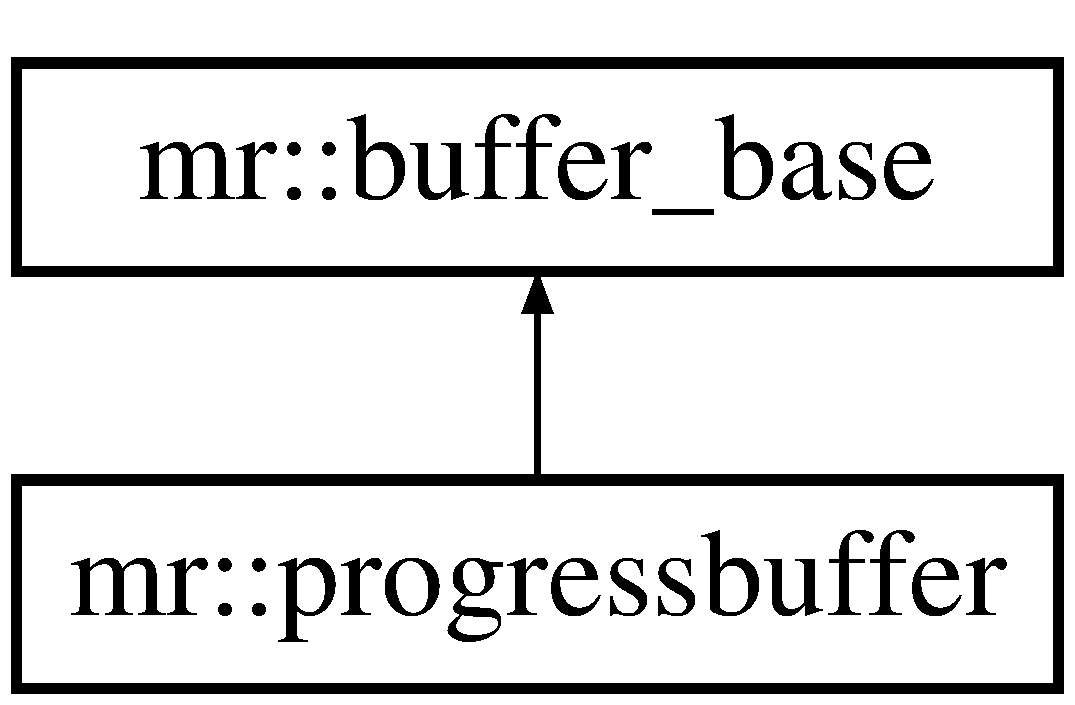
\includegraphics[height=2cm]{structmr_1_1progressbuffer}
\end{center}
\end{figure}
\subsection*{Public Member Functions}
\begin{CompactItemize}
\item 
{\bf progressbuffer} ()
\item 
virtual void {\bf print} (const char $\ast$const s)
\begin{CompactList}\small\item\em virtual function to print string out \item\end{CompactList}\end{CompactItemize}


\subsection{Constructor \& Destructor Documentation}
\index{mr::progressbuffer@{mr::progressbuffer}!progressbuffer@{progressbuffer}}
\index{progressbuffer@{progressbuffer}!mr::progressbuffer@{mr::progressbuffer}}
\subsubsection{\setlength{\rightskip}{0pt plus 5cm}mr::progressbuffer::progressbuffer ()\hspace{0.3cm}{\tt  [inline]}}\label{structmr_1_1progressbuffer_a0}




\subsection{Member Function Documentation}
\index{mr::progressbuffer@{mr::progressbuffer}!print@{print}}
\index{print@{print}!mr::progressbuffer@{mr::progressbuffer}}
\subsubsection{\setlength{\rightskip}{0pt plus 5cm}virtual void mr::progressbuffer::print (const char $\ast$const {\em s})\hspace{0.3cm}{\tt  [inline, virtual]}}\label{structmr_1_1progressbuffer_a1}


virtual function to print string out 



Implements {\bf mr::buffer\_\-base} {\rm (p.\,\pageref{structmr_1_1buffer__base_a3})}.

The documentation for this struct was generated from the following file:\begin{CompactItemize}
\item 
{\bf mr\-Stream.h}\end{CompactItemize}

\section{mr::progressstream Struct Reference}
\label{structmr_1_1progressstream}\index{mr::progressstream@{mr::progressstream}}
{\tt \#include $<$mr\-Stream.h$>$}

\subsection*{Public Member Functions}
\begin{CompactItemize}
\item 
{\bf progressstream} ()
\item 
{\bf $\sim$progressstream} ()
\end{CompactItemize}


\subsection{Constructor \& Destructor Documentation}
\index{mr::progressstream@{mr::progressstream}!progressstream@{progressstream}}
\index{progressstream@{progressstream}!mr::progressstream@{mr::progressstream}}
\subsubsection{\setlength{\rightskip}{0pt plus 5cm}mr::progressstream::progressstream ()\hspace{0.3cm}{\tt  [inline]}}\label{structmr_1_1progressstream_a0}


\index{mr::progressstream@{mr::progressstream}!~progressstream@{$\sim$progressstream}}
\index{~progressstream@{$\sim$progressstream}!mr::progressstream@{mr::progressstream}}
\subsubsection{\setlength{\rightskip}{0pt plus 5cm}mr::progressstream::$\sim${\bf progressstream} ()\hspace{0.3cm}{\tt  [inline]}}\label{structmr_1_1progressstream_a1}




The documentation for this struct was generated from the following file:\begin{CompactItemize}
\item 
{\bf mr\-Stream.h}\end{CompactItemize}

\section{mr::sampler Struct Reference}
\label{structmr_1_1sampler}\index{mr::sampler@{mr::sampler}}
{\tt \#include $<$mr\-Sampler.h$>$}

Inheritance diagram for mr::sampler::\begin{figure}[H]
\begin{center}
\leavevmode
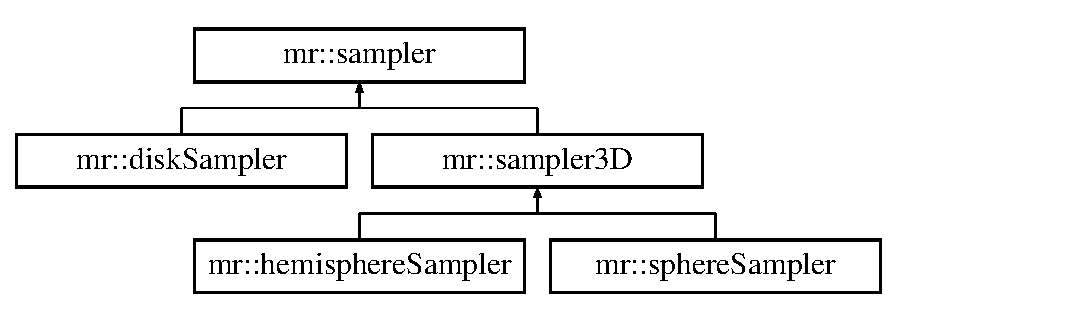
\includegraphics[height=3cm]{structmr_1_1sampler}
\end{center}
\end{figure}
\subsection*{Public Member Functions}
\begin{CompactItemize}
\item 
{\bf sampler} ()
\begin{CompactList}\small\item\em Constructor for adaptive sampling. \item\end{CompactList}\item 
{\bf sampler} (const mi\-Uint \&num\-Samples)
\begin{CompactList}\small\item\em Constructor for fixed sampling. num\-Samples HAS to be mi\-Uint\&. \item\end{CompactList}\item 
{\bf $\sim$sampler} ()
\item 
const int {\bf count} ()
\begin{CompactList}\small\item\em Returns the number of samples taken so far. \item\end{CompactList}\end{CompactItemize}
\subsection*{Public Attributes}
\begin{CompactItemize}
\item 
const mi\-Uint $\ast$ {\bf max\-Samples}
\item 
int {\bf counter}
\end{CompactItemize}


\subsection{Constructor \& Destructor Documentation}
\index{mr::sampler@{mr::sampler}!sampler@{sampler}}
\index{sampler@{sampler}!mr::sampler@{mr::sampler}}
\subsubsection{\setlength{\rightskip}{0pt plus 5cm}mr::sampler::sampler ()\hspace{0.3cm}{\tt  [inline]}}\label{structmr_1_1sampler_a0}


Constructor for adaptive sampling. 

\index{mr::sampler@{mr::sampler}!sampler@{sampler}}
\index{sampler@{sampler}!mr::sampler@{mr::sampler}}
\subsubsection{\setlength{\rightskip}{0pt plus 5cm}mr::sampler::sampler (const mi\-Uint \& {\em num\-Samples})\hspace{0.3cm}{\tt  [inline]}}\label{structmr_1_1sampler_a1}


Constructor for fixed sampling. num\-Samples HAS to be mi\-Uint\&. 

\index{mr::sampler@{mr::sampler}!~sampler@{$\sim$sampler}}
\index{~sampler@{$\sim$sampler}!mr::sampler@{mr::sampler}}
\subsubsection{\setlength{\rightskip}{0pt plus 5cm}mr::sampler::$\sim${\bf sampler} ()\hspace{0.3cm}{\tt  [inline]}}\label{structmr_1_1sampler_a2}




\subsection{Member Function Documentation}
\index{mr::sampler@{mr::sampler}!count@{count}}
\index{count@{count}!mr::sampler@{mr::sampler}}
\subsubsection{\setlength{\rightskip}{0pt plus 5cm}const int mr::sampler::count ()\hspace{0.3cm}{\tt  [inline]}}\label{structmr_1_1sampler_a3}


Returns the number of samples taken so far. 



\subsection{Member Data Documentation}
\index{mr::sampler@{mr::sampler}!counter@{counter}}
\index{counter@{counter}!mr::sampler@{mr::sampler}}
\subsubsection{\setlength{\rightskip}{0pt plus 5cm}int {\bf mr::sampler::counter}}\label{structmr_1_1sampler_o1}


\index{mr::sampler@{mr::sampler}!maxSamples@{maxSamples}}
\index{maxSamples@{maxSamples}!mr::sampler@{mr::sampler}}
\subsubsection{\setlength{\rightskip}{0pt plus 5cm}const mi\-Uint$\ast$ {\bf mr::sampler::max\-Samples}}\label{structmr_1_1sampler_o0}




The documentation for this struct was generated from the following file:\begin{CompactItemize}
\item 
{\bf mr\-Sampler.h}\end{CompactItemize}

\section{mr::sampler3D Struct Reference}
\label{structmr_1_1sampler3D}\index{mr::sampler3D@{mr::sampler3D}}
{\tt \#include $<$mr\-Sampler.h$>$}

Inheritance diagram for mr::sampler3D::\begin{figure}[H]
\begin{center}
\leavevmode
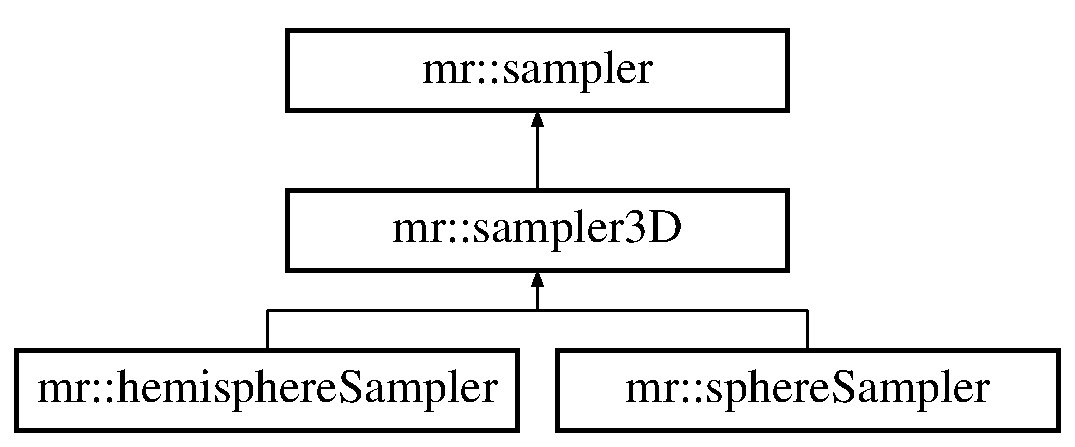
\includegraphics[height=3cm]{structmr_1_1sampler3D}
\end{center}
\end{figure}
\subsection*{Public Member Functions}
\begin{CompactItemize}
\item 
{\bf sampler3D} ()
\begin{CompactList}\small\item\em Constructor for adaptive sampling. \item\end{CompactList}\item 
{\bf sampler3D} (const mi\-Uint \&num\-Samples)
\begin{CompactList}\small\item\em Constructor for fixed sampling. num\-Samples HAS to be mi\-Uint\&. \item\end{CompactList}\item 
{\bf $\sim$sampler3D} ()
\item 
mi\-Vector \& {\bf direction} ()
\begin{CompactList}\small\item\em Return direction for this sample. \item\end{CompactList}\end{CompactItemize}
\subsection*{Public Attributes}
\begin{CompactItemize}
\item 
double {\bf samples} [2]
\begin{CompactList}\small\item\em mi\_\-sample() auxiliaries to store 2 random numbers \item\end{CompactList}\item 
mi\-Vector {\bf dir}
\begin{CompactList}\small\item\em Final sampling direction for this sample. \item\end{CompactList}\end{CompactItemize}


\subsection{Constructor \& Destructor Documentation}
\index{mr::sampler3D@{mr::sampler3D}!sampler3D@{sampler3D}}
\index{sampler3D@{sampler3D}!mr::sampler3D@{mr::sampler3D}}
\subsubsection{\setlength{\rightskip}{0pt plus 5cm}mr::sampler3D::sampler3D ()\hspace{0.3cm}{\tt  [inline]}}\label{structmr_1_1sampler3D_a0}


Constructor for adaptive sampling. 

\index{mr::sampler3D@{mr::sampler3D}!sampler3D@{sampler3D}}
\index{sampler3D@{sampler3D}!mr::sampler3D@{mr::sampler3D}}
\subsubsection{\setlength{\rightskip}{0pt plus 5cm}mr::sampler3D::sampler3D (const mi\-Uint \& {\em num\-Samples})\hspace{0.3cm}{\tt  [inline]}}\label{structmr_1_1sampler3D_a1}


Constructor for fixed sampling. num\-Samples HAS to be mi\-Uint\&. 

\index{mr::sampler3D@{mr::sampler3D}!~sampler3D@{$\sim$sampler3D}}
\index{~sampler3D@{$\sim$sampler3D}!mr::sampler3D@{mr::sampler3D}}
\subsubsection{\setlength{\rightskip}{0pt plus 5cm}mr::sampler3D::$\sim${\bf sampler3D} ()\hspace{0.3cm}{\tt  [inline]}}\label{structmr_1_1sampler3D_a2}




\subsection{Member Function Documentation}
\index{mr::sampler3D@{mr::sampler3D}!direction@{direction}}
\index{direction@{direction}!mr::sampler3D@{mr::sampler3D}}
\subsubsection{\setlength{\rightskip}{0pt plus 5cm}mi\-Vector\& mr::sampler3D::direction ()\hspace{0.3cm}{\tt  [inline]}}\label{structmr_1_1sampler3D_a3}


Return direction for this sample. 



\subsection{Member Data Documentation}
\index{mr::sampler3D@{mr::sampler3D}!dir@{dir}}
\index{dir@{dir}!mr::sampler3D@{mr::sampler3D}}
\subsubsection{\setlength{\rightskip}{0pt plus 5cm}mi\-Vector {\bf mr::sampler3D::dir}}\label{structmr_1_1sampler3D_o1}


Final sampling direction for this sample. 

\index{mr::sampler3D@{mr::sampler3D}!samples@{samples}}
\index{samples@{samples}!mr::sampler3D@{mr::sampler3D}}
\subsubsection{\setlength{\rightskip}{0pt plus 5cm}double {\bf mr::sampler3D::samples}[2]}\label{structmr_1_1sampler3D_o0}


mi\_\-sample() auxiliaries to store 2 random numbers 



The documentation for this struct was generated from the following file:\begin{CompactItemize}
\item 
{\bf mr\-Sampler.h}\end{CompactItemize}

\section{mr::simple\_\-timer Class Reference}
\label{classmr_1_1simple__timer}\index{mr::simple_timer@{mr::simple\_\-timer}}
{\tt \#include $<$mr\-Profile.h$>$}

Inheritance diagram for mr::simple\_\-timer::\begin{figure}[H]
\begin{center}
\leavevmode
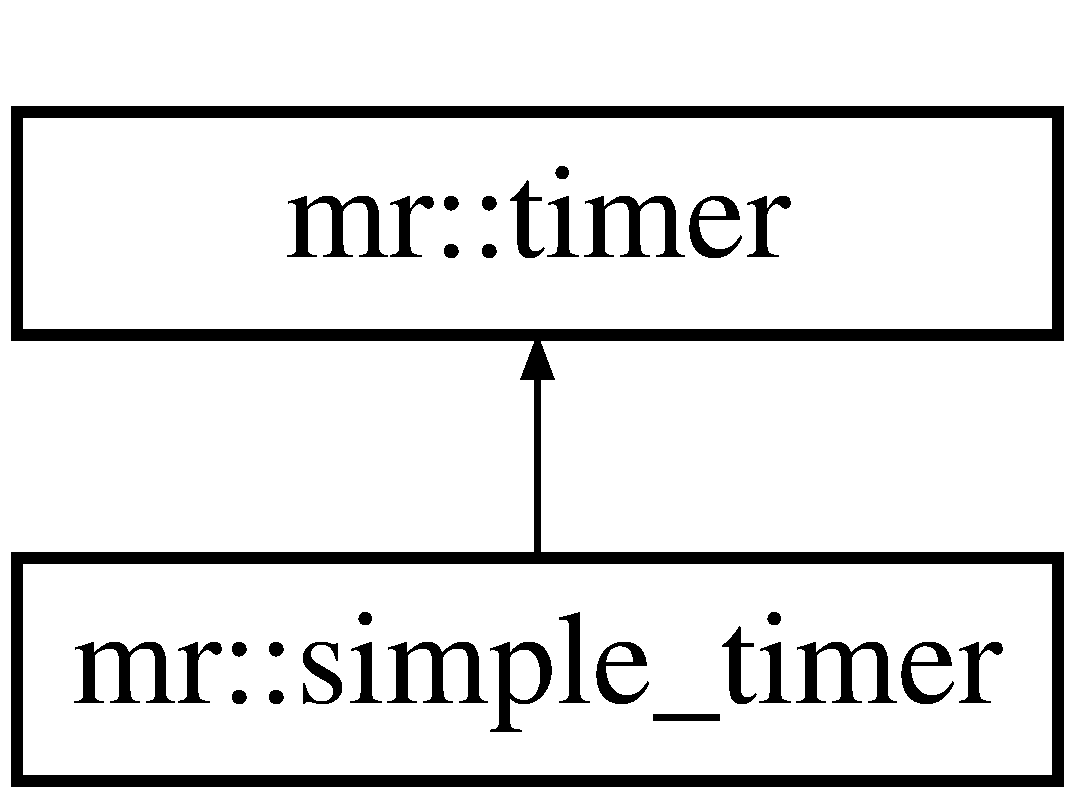
\includegraphics[height=2cm]{classmr_1_1simple__timer}
\end{center}
\end{figure}


\subsection{Detailed Description}
Very simple class/macro for profiling stuff... Just use MR\_\-TIME\_\-IT macro and enclose area in \{\}, like...



\footnotesize\begin{verbatim}      {
        MR_TIME_IT;
         ....stuff to profile...
      }  // here it will print result
\end{verbatim}
\normalsize




The documentation for this class was generated from the following file:\begin{CompactItemize}
\item 
{\bf mr\-Profile.h}\end{CompactItemize}

\section{mr::SPerlin Class Reference}
\label{classmr_1_1SPerlin}\index{mr::SPerlin@{mr::SPerlin}}
Perlin Class returning a mi\-Scalar.  


{\tt \#include $<$mr\-Perlin.h$>$}

\subsection*{Static Public Member Functions}
\begin{CompactItemize}
\item 
mi\-Scalar {\bf snoise} (mi\-Scalar x)
\item 
mi\-Scalar {\bf snoise} (mi\-Scalar x, mi\-Scalar y)
\item 
mi\-Scalar {\bf snoise} (mi\-Scalar x, mi\-Scalar y, mi\-Scalar z)
\item 
mi\-Scalar {\bf snoise} (mi\-Scalar x, mi\-Scalar y, mi\-Scalar z, mi\-Scalar t)
\item 
mi\-Scalar {\bf snoise} (const {\bf vector2d} \&P)
\item 
mi\-Scalar {\bf snoise} (const {\bf point} \&P)
\item 
mi\-Scalar {\bf snoise} (const {\bf point} \&P, const mi\-Scalar t)
\item 
mi\-Scalar {\bf noise} (const mi\-Scalar x)
\item 
mi\-Scalar {\bf noise} (const mi\-Scalar x, const mi\-Scalar y)
\item 
mi\-Scalar {\bf noise} (const mi\-Scalar x, const mi\-Scalar y, const mi\-Scalar z)
\item 
mi\-Scalar {\bf noise} (const mi\-Scalar x, const mi\-Scalar y, const mi\-Scalar z, const mi\-Scalar t)
\item 
mi\-Scalar {\bf noise} (const {\bf vector2d} \&P)
\item 
mi\-Scalar {\bf noise} (const {\bf point} \&P)
\item 
mi\-Scalar {\bf noise} (const {\bf point} \&P, const mi\-Scalar t)
\item 
mi\-Scalar {\bf pnoise} (const mi\-Scalar xi, const mi\-Scalar period)
\item 
mi\-Scalar {\bf pnoise} (const mi\-Scalar xi, const mi\-Scalar yi, const mi\-Scalar w, const mi\-Scalar h)
\item 
mi\-Scalar {\bf pnoise} (const mi\-Scalar xi, const mi\-Scalar yi, const mi\-Scalar zi, const mi\-Scalar w, const mi\-Scalar h, const mi\-Scalar d)
\item 
mi\-Scalar {\bf pnoise} (const mi\-Scalar xi, const mi\-Scalar yi, const mi\-Scalar zi, const mi\-Scalar ti, const mi\-Scalar w, const mi\-Scalar h, const mi\-Scalar d, const mi\-Scalar p)
\item 
mi\-Scalar {\bf pnoise} (const {\bf vector2d} \&P, const {\bf vector2d} \&period)
\item 
mi\-Scalar {\bf pnoise} (const {\bf point} \&P, const {\bf vector} \&period)
\item 
mi\-Scalar {\bf pnoise} (const {\bf point} \&P, const mi\-Scalar t, const {\bf vector} \&Pperiod, const mi\-Scalar tperiod)
\item 
mi\-Scalar {\bf spnoise} (const mi\-Scalar xi, const mi\-Scalar period)
\item 
mi\-Scalar {\bf spnoise} (const mi\-Scalar xi, const mi\-Scalar yi, const mi\-Scalar w, const mi\-Scalar h)
\item 
mi\-Scalar {\bf spnoise} (const mi\-Scalar xi, const mi\-Scalar yi, const mi\-Scalar zi, const mi\-Scalar w, const mi\-Scalar h, const mi\-Scalar d)
\item 
mi\-Scalar {\bf spnoise} (const mi\-Scalar xi, const mi\-Scalar yi, const mi\-Scalar zi, const mi\-Scalar ti, const mi\-Scalar w, const mi\-Scalar h, const mi\-Scalar d, const mi\-Scalar p)
\item 
mi\-Scalar {\bf spnoise} (const {\bf vector2d} \&P, const {\bf vector2d} \&period)
\item 
mi\-Scalar {\bf spnoise} (const {\bf point} \&P, const {\bf vector} \&period)
\item 
mi\-Scalar {\bf spnoise} (const {\bf point} \&P, const mi\-Scalar t, const {\bf vector} \&Pperiod, const mi\-Scalar tperiod)
\end{CompactItemize}


\subsection{Detailed Description}
Perlin Class returning a mi\-Scalar. 

\begin{Desc}
\item[{\bf Todo}]: rewrite {\bf snoise( 4 channels)}{\rm (p.\,\pageref{mrRman__notes_8h_a14})} as the indexes are wrong and so is the gradient. 

: Make noise functions that return the gradient?\end{Desc}




\subsection{Member Function Documentation}
\index{mr::SPerlin@{mr::SPerlin}!noise@{noise}}
\index{noise@{noise}!mr::SPerlin@{mr::SPerlin}}
\subsubsection{\setlength{\rightskip}{0pt plus 5cm}mi\-Scalar mr::SPerlin::noise (const {\bf point} \& {\em P}, const mi\-Scalar {\em t})\hspace{0.3cm}{\tt  [inline, static]}}\label{classmr_1_1SPerlin_e13}


\index{mr::SPerlin@{mr::SPerlin}!noise@{noise}}
\index{noise@{noise}!mr::SPerlin@{mr::SPerlin}}
\subsubsection{\setlength{\rightskip}{0pt plus 5cm}mi\-Scalar mr::SPerlin::noise (const {\bf point} \& {\em P})\hspace{0.3cm}{\tt  [inline, static]}}\label{classmr_1_1SPerlin_e12}


\index{mr::SPerlin@{mr::SPerlin}!noise@{noise}}
\index{noise@{noise}!mr::SPerlin@{mr::SPerlin}}
\subsubsection{\setlength{\rightskip}{0pt plus 5cm}mi\-Scalar mr::SPerlin::noise (const {\bf vector2d} \& {\em P})\hspace{0.3cm}{\tt  [inline, static]}}\label{classmr_1_1SPerlin_e11}


\index{mr::SPerlin@{mr::SPerlin}!noise@{noise}}
\index{noise@{noise}!mr::SPerlin@{mr::SPerlin}}
\subsubsection{\setlength{\rightskip}{0pt plus 5cm}mi\-Scalar mr::SPerlin::noise (const mi\-Scalar {\em x}, const mi\-Scalar {\em y}, const mi\-Scalar {\em z}, const mi\-Scalar {\em t})\hspace{0.3cm}{\tt  [inline, static]}}\label{classmr_1_1SPerlin_e10}


\index{mr::SPerlin@{mr::SPerlin}!noise@{noise}}
\index{noise@{noise}!mr::SPerlin@{mr::SPerlin}}
\subsubsection{\setlength{\rightskip}{0pt plus 5cm}mi\-Scalar mr::SPerlin::noise (const mi\-Scalar {\em x}, const mi\-Scalar {\em y}, const mi\-Scalar {\em z})\hspace{0.3cm}{\tt  [inline, static]}}\label{classmr_1_1SPerlin_e9}


\index{mr::SPerlin@{mr::SPerlin}!noise@{noise}}
\index{noise@{noise}!mr::SPerlin@{mr::SPerlin}}
\subsubsection{\setlength{\rightskip}{0pt plus 5cm}mi\-Scalar mr::SPerlin::noise (const mi\-Scalar {\em x}, const mi\-Scalar {\em y})\hspace{0.3cm}{\tt  [inline, static]}}\label{classmr_1_1SPerlin_e8}


\index{mr::SPerlin@{mr::SPerlin}!noise@{noise}}
\index{noise@{noise}!mr::SPerlin@{mr::SPerlin}}
\subsubsection{\setlength{\rightskip}{0pt plus 5cm}mi\-Scalar mr::SPerlin::noise (const mi\-Scalar {\em x})\hspace{0.3cm}{\tt  [inline, static]}}\label{classmr_1_1SPerlin_e7}


\index{mr::SPerlin@{mr::SPerlin}!pnoise@{pnoise}}
\index{pnoise@{pnoise}!mr::SPerlin@{mr::SPerlin}}
\subsubsection{\setlength{\rightskip}{0pt plus 5cm}mi\-Scalar mr::SPerlin::pnoise (const {\bf point} \& {\em P}, const mi\-Scalar {\em t}, const {\bf vector} \& {\em Pperiod}, const mi\-Scalar {\em tperiod})\hspace{0.3cm}{\tt  [inline, static]}}\label{classmr_1_1SPerlin_e20}


\index{mr::SPerlin@{mr::SPerlin}!pnoise@{pnoise}}
\index{pnoise@{pnoise}!mr::SPerlin@{mr::SPerlin}}
\subsubsection{\setlength{\rightskip}{0pt plus 5cm}mi\-Scalar mr::SPerlin::pnoise (const {\bf point} \& {\em P}, const {\bf vector} \& {\em period})\hspace{0.3cm}{\tt  [inline, static]}}\label{classmr_1_1SPerlin_e19}


\index{mr::SPerlin@{mr::SPerlin}!pnoise@{pnoise}}
\index{pnoise@{pnoise}!mr::SPerlin@{mr::SPerlin}}
\subsubsection{\setlength{\rightskip}{0pt plus 5cm}mi\-Scalar mr::SPerlin::pnoise (const {\bf vector2d} \& {\em P}, const {\bf vector2d} \& {\em period})\hspace{0.3cm}{\tt  [inline, static]}}\label{classmr_1_1SPerlin_e18}


\index{mr::SPerlin@{mr::SPerlin}!pnoise@{pnoise}}
\index{pnoise@{pnoise}!mr::SPerlin@{mr::SPerlin}}
\subsubsection{\setlength{\rightskip}{0pt plus 5cm}mi\-Scalar mr::SPerlin::pnoise (const mi\-Scalar {\em xi}, const mi\-Scalar {\em yi}, const mi\-Scalar {\em zi}, const mi\-Scalar {\em ti}, const mi\-Scalar {\em w}, const mi\-Scalar {\em h}, const mi\-Scalar {\em d}, const mi\-Scalar {\em p})\hspace{0.3cm}{\tt  [inline, static]}}\label{classmr_1_1SPerlin_e17}


\index{mr::SPerlin@{mr::SPerlin}!pnoise@{pnoise}}
\index{pnoise@{pnoise}!mr::SPerlin@{mr::SPerlin}}
\subsubsection{\setlength{\rightskip}{0pt plus 5cm}mi\-Scalar mr::SPerlin::pnoise (const mi\-Scalar {\em xi}, const mi\-Scalar {\em yi}, const mi\-Scalar {\em zi}, const mi\-Scalar {\em w}, const mi\-Scalar {\em h}, const mi\-Scalar {\em d})\hspace{0.3cm}{\tt  [inline, static]}}\label{classmr_1_1SPerlin_e16}


\index{mr::SPerlin@{mr::SPerlin}!pnoise@{pnoise}}
\index{pnoise@{pnoise}!mr::SPerlin@{mr::SPerlin}}
\subsubsection{\setlength{\rightskip}{0pt plus 5cm}mi\-Scalar mr::SPerlin::pnoise (const mi\-Scalar {\em xi}, const mi\-Scalar {\em yi}, const mi\-Scalar {\em w}, const mi\-Scalar {\em h})\hspace{0.3cm}{\tt  [inline, static]}}\label{classmr_1_1SPerlin_e15}


\index{mr::SPerlin@{mr::SPerlin}!pnoise@{pnoise}}
\index{pnoise@{pnoise}!mr::SPerlin@{mr::SPerlin}}
\subsubsection{\setlength{\rightskip}{0pt plus 5cm}mi\-Scalar mr::SPerlin::pnoise (const mi\-Scalar {\em xi}, const mi\-Scalar {\em period})\hspace{0.3cm}{\tt  [inline, static]}}\label{classmr_1_1SPerlin_e14}


\index{mr::SPerlin@{mr::SPerlin}!snoise@{snoise}}
\index{snoise@{snoise}!mr::SPerlin@{mr::SPerlin}}
\subsubsection{\setlength{\rightskip}{0pt plus 5cm}mi\-Scalar mr::SPerlin::snoise (const {\bf point} \& {\em P}, const mi\-Scalar {\em t})\hspace{0.3cm}{\tt  [inline, static]}}\label{classmr_1_1SPerlin_e6}


\index{mr::SPerlin@{mr::SPerlin}!snoise@{snoise}}
\index{snoise@{snoise}!mr::SPerlin@{mr::SPerlin}}
\subsubsection{\setlength{\rightskip}{0pt plus 5cm}mi\-Scalar mr::SPerlin::snoise (const {\bf point} \& {\em P})\hspace{0.3cm}{\tt  [inline, static]}}\label{classmr_1_1SPerlin_e5}


\index{mr::SPerlin@{mr::SPerlin}!snoise@{snoise}}
\index{snoise@{snoise}!mr::SPerlin@{mr::SPerlin}}
\subsubsection{\setlength{\rightskip}{0pt plus 5cm}mi\-Scalar mr::SPerlin::snoise (const {\bf vector2d} \& {\em P})\hspace{0.3cm}{\tt  [inline, static]}}\label{classmr_1_1SPerlin_e4}


\index{mr::SPerlin@{mr::SPerlin}!snoise@{snoise}}
\index{snoise@{snoise}!mr::SPerlin@{mr::SPerlin}}
\subsubsection{\setlength{\rightskip}{0pt plus 5cm}mi\-Scalar mr::SPerlin::snoise (mi\-Scalar {\em x}, mi\-Scalar {\em y}, mi\-Scalar {\em z}, mi\-Scalar {\em t})\hspace{0.3cm}{\tt  [inline, static]}}\label{classmr_1_1SPerlin_e3}


\index{mr::SPerlin@{mr::SPerlin}!snoise@{snoise}}
\index{snoise@{snoise}!mr::SPerlin@{mr::SPerlin}}
\subsubsection{\setlength{\rightskip}{0pt plus 5cm}mi\-Scalar mr::SPerlin::snoise (mi\-Scalar {\em x}, mi\-Scalar {\em y}, mi\-Scalar {\em z})\hspace{0.3cm}{\tt  [inline, static]}}\label{classmr_1_1SPerlin_e2}


\index{mr::SPerlin@{mr::SPerlin}!snoise@{snoise}}
\index{snoise@{snoise}!mr::SPerlin@{mr::SPerlin}}
\subsubsection{\setlength{\rightskip}{0pt plus 5cm}mi\-Scalar mr::SPerlin::snoise (mi\-Scalar {\em x}, mi\-Scalar {\em y})\hspace{0.3cm}{\tt  [inline, static]}}\label{classmr_1_1SPerlin_e1}


\index{mr::SPerlin@{mr::SPerlin}!snoise@{snoise}}
\index{snoise@{snoise}!mr::SPerlin@{mr::SPerlin}}
\subsubsection{\setlength{\rightskip}{0pt plus 5cm}mi\-Scalar mr::SPerlin::snoise (mi\-Scalar {\em x})\hspace{0.3cm}{\tt  [inline, static]}}\label{classmr_1_1SPerlin_e0}


\index{mr::SPerlin@{mr::SPerlin}!spnoise@{spnoise}}
\index{spnoise@{spnoise}!mr::SPerlin@{mr::SPerlin}}
\subsubsection{\setlength{\rightskip}{0pt plus 5cm}mi\-Scalar mr::SPerlin::spnoise (const {\bf point} \& {\em P}, const mi\-Scalar {\em t}, const {\bf vector} \& {\em Pperiod}, const mi\-Scalar {\em tperiod})\hspace{0.3cm}{\tt  [inline, static]}}\label{classmr_1_1SPerlin_e27}


\index{mr::SPerlin@{mr::SPerlin}!spnoise@{spnoise}}
\index{spnoise@{spnoise}!mr::SPerlin@{mr::SPerlin}}
\subsubsection{\setlength{\rightskip}{0pt plus 5cm}mi\-Scalar mr::SPerlin::spnoise (const {\bf point} \& {\em P}, const {\bf vector} \& {\em period})\hspace{0.3cm}{\tt  [inline, static]}}\label{classmr_1_1SPerlin_e26}


\index{mr::SPerlin@{mr::SPerlin}!spnoise@{spnoise}}
\index{spnoise@{spnoise}!mr::SPerlin@{mr::SPerlin}}
\subsubsection{\setlength{\rightskip}{0pt plus 5cm}mi\-Scalar mr::SPerlin::spnoise (const {\bf vector2d} \& {\em P}, const {\bf vector2d} \& {\em period})\hspace{0.3cm}{\tt  [inline, static]}}\label{classmr_1_1SPerlin_e25}


\index{mr::SPerlin@{mr::SPerlin}!spnoise@{spnoise}}
\index{spnoise@{spnoise}!mr::SPerlin@{mr::SPerlin}}
\subsubsection{\setlength{\rightskip}{0pt plus 5cm}mi\-Scalar mr::SPerlin::spnoise (const mi\-Scalar {\em xi}, const mi\-Scalar {\em yi}, const mi\-Scalar {\em zi}, const mi\-Scalar {\em ti}, const mi\-Scalar {\em w}, const mi\-Scalar {\em h}, const mi\-Scalar {\em d}, const mi\-Scalar {\em p})\hspace{0.3cm}{\tt  [inline, static]}}\label{classmr_1_1SPerlin_e24}


\index{mr::SPerlin@{mr::SPerlin}!spnoise@{spnoise}}
\index{spnoise@{spnoise}!mr::SPerlin@{mr::SPerlin}}
\subsubsection{\setlength{\rightskip}{0pt plus 5cm}mi\-Scalar mr::SPerlin::spnoise (const mi\-Scalar {\em xi}, const mi\-Scalar {\em yi}, const mi\-Scalar {\em zi}, const mi\-Scalar {\em w}, const mi\-Scalar {\em h}, const mi\-Scalar {\em d})\hspace{0.3cm}{\tt  [inline, static]}}\label{classmr_1_1SPerlin_e23}


\index{mr::SPerlin@{mr::SPerlin}!spnoise@{spnoise}}
\index{spnoise@{spnoise}!mr::SPerlin@{mr::SPerlin}}
\subsubsection{\setlength{\rightskip}{0pt plus 5cm}mi\-Scalar mr::SPerlin::spnoise (const mi\-Scalar {\em xi}, const mi\-Scalar {\em yi}, const mi\-Scalar {\em w}, const mi\-Scalar {\em h})\hspace{0.3cm}{\tt  [inline, static]}}\label{classmr_1_1SPerlin_e22}


\index{mr::SPerlin@{mr::SPerlin}!spnoise@{spnoise}}
\index{spnoise@{spnoise}!mr::SPerlin@{mr::SPerlin}}
\subsubsection{\setlength{\rightskip}{0pt plus 5cm}mi\-Scalar mr::SPerlin::spnoise (const mi\-Scalar {\em xi}, const mi\-Scalar {\em period})\hspace{0.3cm}{\tt  [inline, static]}}\label{classmr_1_1SPerlin_e21}




The documentation for this class was generated from the following file:\begin{CompactItemize}
\item 
{\bf mr\-Perlin.h}\end{CompactItemize}

\section{mr::sphere\-Sampler Class Reference}
\label{classmr_1_1sphereSampler}\index{mr::sphereSampler@{mr::sphereSampler}}
Sample spherically or partially around a sphere.  


{\tt \#include $<$mr\-Sampler.h$>$}

Inheritance diagram for mr::sphere\-Sampler::\begin{figure}[H]
\begin{center}
\leavevmode
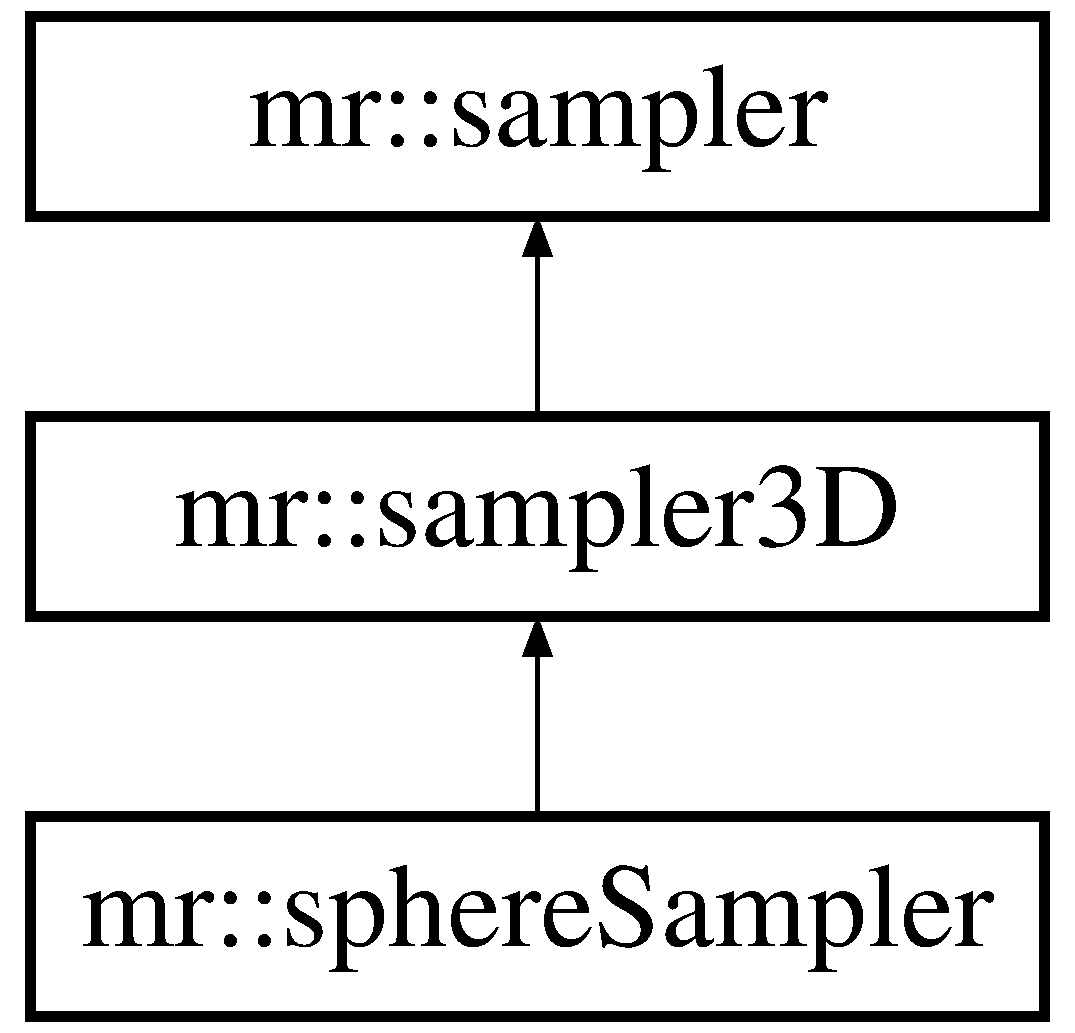
\includegraphics[height=3cm]{classmr_1_1sphereSampler}
\end{center}
\end{figure}
\subsection*{Public Member Functions}
\begin{CompactItemize}
\item 
{\bf sphere\-Sampler} (const mi\-Vector \&Nin, const mi\-Scalar sphere\-Percent=1.0f)
\item 
{\bf sphere\-Sampler} (const mi\-Vector \&Nin, const mi\-Uint \&num\-Samples, const mi\-Scalar sphere\-Percent=1.0f)
\item 
{\bf $\sim$sphere\-Sampler} ()
\begin{CompactList}\small\item\em Destructor. \item\end{CompactList}\item 
const mi\-Scalar {\bf weight} ()
\item 
bool {\bf uniform} (const mi\-State $\ast$const state)
\begin{CompactList}\small\item\em Get one sample using a uniform distribution or return false. \item\end{CompactList}\end{CompactItemize}
\subsection*{Protected Member Functions}
\begin{CompactItemize}
\item 
void {\bf calculate\-Direction} ()
\item 
void {\bf uniform\-Distribution} ()
\end{CompactItemize}


\subsection{Detailed Description}
Sample spherically or partially around a sphere. 



\subsection{Constructor \& Destructor Documentation}
\index{mr::sphereSampler@{mr::sphere\-Sampler}!sphereSampler@{sphereSampler}}
\index{sphereSampler@{sphereSampler}!mr::sphereSampler@{mr::sphere\-Sampler}}
\subsubsection{\setlength{\rightskip}{0pt plus 5cm}mr::sphere\-Sampler::sphere\-Sampler (const mi\-Vector \& {\em Nin}, const mi\-Scalar {\em sphere\-Percent} = 1.0f)\hspace{0.3cm}{\tt  [inline]}}\label{classmr_1_1sphereSampler_a0}


Constructor. Nin is the direction to sample around. sphere\-Percent is percentage of sphere to cover. If sphere percent is 1, Nin is irrelevant. This call is to be used when sampling adaptively (ie. the number of samples to be taken are not known or may vary, or you may exit the loop early). \index{mr::sphereSampler@{mr::sphere\-Sampler}!sphereSampler@{sphereSampler}}
\index{sphereSampler@{sphereSampler}!mr::sphereSampler@{mr::sphere\-Sampler}}
\subsubsection{\setlength{\rightskip}{0pt plus 5cm}mr::sphere\-Sampler::sphere\-Sampler (const mi\-Vector \& {\em Nin}, const mi\-Uint \& {\em num\-Samples}, const mi\-Scalar {\em sphere\-Percent} = 1.0f)\hspace{0.3cm}{\tt  [inline]}}\label{classmr_1_1sphereSampler_a1}


Constructor. Nin is the direction to sample around. sphere\-Percent is percentage of sphere to cover. If sphere percent is 1, Nin is irrelevant. num\-Samples is the number of samples to take. It HAS to be mi\-Uint\& \index{mr::sphereSampler@{mr::sphere\-Sampler}!~sphereSampler@{$\sim$sphereSampler}}
\index{~sphereSampler@{$\sim$sphereSampler}!mr::sphereSampler@{mr::sphere\-Sampler}}
\subsubsection{\setlength{\rightskip}{0pt plus 5cm}mr::sphere\-Sampler::$\sim${\bf sphere\-Sampler} ()\hspace{0.3cm}{\tt  [inline]}}\label{classmr_1_1sphereSampler_a2}


Destructor. 



\subsection{Member Function Documentation}
\index{mr::sphereSampler@{mr::sphere\-Sampler}!calculateDirection@{calculateDirection}}
\index{calculateDirection@{calculateDirection}!mr::sphereSampler@{mr::sphere\-Sampler}}
\subsubsection{\setlength{\rightskip}{0pt plus 5cm}void mr::sphere\-Sampler::calculate\-Direction ()\hspace{0.3cm}{\tt  [inline, protected]}}\label{classmr_1_1sphereSampler_b0}


\index{mr::sphereSampler@{mr::sphere\-Sampler}!uniform@{uniform}}
\index{uniform@{uniform}!mr::sphereSampler@{mr::sphere\-Sampler}}
\subsubsection{\setlength{\rightskip}{0pt plus 5cm}bool mr::sphere\-Sampler::uniform (const mi\-State $\ast$const {\em state})\hspace{0.3cm}{\tt  [inline]}}\label{classmr_1_1sphereSampler_a4}


Get one sample using a uniform distribution or return false. 

\index{mr::sphereSampler@{mr::sphere\-Sampler}!uniformDistribution@{uniformDistribution}}
\index{uniformDistribution@{uniformDistribution}!mr::sphereSampler@{mr::sphere\-Sampler}}
\subsubsection{\setlength{\rightskip}{0pt plus 5cm}void mr::sphere\-Sampler::uniform\-Distribution ()\hspace{0.3cm}{\tt  [inline, protected]}}\label{classmr_1_1sphereSampler_b1}


\index{mr::sphereSampler@{mr::sphere\-Sampler}!weight@{weight}}
\index{weight@{weight}!mr::sphereSampler@{mr::sphere\-Sampler}}
\subsubsection{\setlength{\rightskip}{0pt plus 5cm}const mi\-Scalar mr::sphere\-Sampler::weight ()\hspace{0.3cm}{\tt  [inline]}}\label{classmr_1_1sphereSampler_a3}


This returns a weight (dot product) of the sample with respect to the original Nin vector. 

The documentation for this class was generated from the following file:\begin{CompactItemize}
\item 
{\bf mr\-Sampler.h}\end{CompactItemize}

\section{mr::base::sub Struct Reference}
\label{structmr_1_1base_1_1sub}\index{mr::base::sub@{mr::base::sub}}
{\tt \#include $<$mr\-Base.h$>$}

\subsection*{Static Public Member Functions}
\begin{CompactItemize}
\item 
template$<$class ta\_\-a, class ta\_\-b$>$ const double {\bf Evaluate} (const unsigned short i, const ta\_\-a \&A, const ta\_\-b \&B)
\end{CompactItemize}


\subsection{Member Function Documentation}
\index{mr::base::sub@{mr::base::sub}!Evaluate@{Evaluate}}
\index{Evaluate@{Evaluate}!mr::base::sub@{mr::base::sub}}
\subsubsection{\setlength{\rightskip}{0pt plus 5cm}template$<$class ta\_\-a, class ta\_\-b$>$ const double mr::base::sub::Evaluate (const unsigned short {\em i}, const ta\_\-a \& {\em A}, const ta\_\-b \& {\em B})\hspace{0.3cm}{\tt  [inline, static]}}\label{structmr_1_1base_1_1sub_e0}




The documentation for this struct was generated from the following file:\begin{CompactItemize}
\item 
{\bf mr\-Base.h}\end{CompactItemize}

\section{mr::distances::Superquadratic Struct Reference}
\label{structmr_1_1distances_1_1Superquadratic}\index{mr::distances::Superquadratic@{mr::distances::Superquadratic}}
Functor to calculate superquadratic distance.  


{\tt \#include $<$mr\-Distances.h$>$}

Inheritance diagram for mr::distances::Superquadratic::\begin{figure}[H]
\begin{center}
\leavevmode
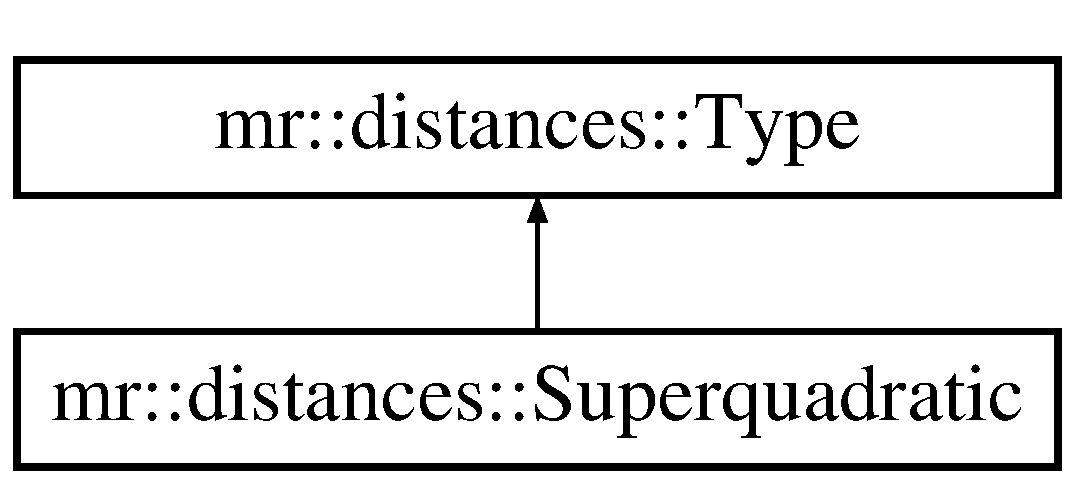
\includegraphics[height=2cm]{structmr_1_1distances_1_1Superquadratic}
\end{center}
\end{figure}
\subsection*{Public Member Functions}
\begin{CompactItemize}
\item 
mi\-Scalar {\bf operator()} (const {\bf vector} \&d) const 
\item 
mi\-Scalar {\bf operator()} (const {\bf vector} \&d, const {\bf vector} \&s) const 
\end{CompactItemize}


\subsection{Detailed Description}
Functor to calculate superquadratic distance. 



\subsection{Member Function Documentation}
\index{mr::distances::Superquadratic@{mr::distances::Superquadratic}!operator()@{operator()}}
\index{operator()@{operator()}!mr::distances::Superquadratic@{mr::distances::Superquadratic}}
\subsubsection{\setlength{\rightskip}{0pt plus 5cm}mi\-Scalar mr::distances::Superquadratic::operator() (const {\bf vector} \& {\em d}, const {\bf vector} \& {\em s}) const\hspace{0.3cm}{\tt  [inline, virtual]}}\label{structmr_1_1distances_1_1Superquadratic_a1}




Implements {\bf mr::distances::Type} {\rm (p.\,\pageref{structmr_1_1distances_1_1Type_a1})}.\index{mr::distances::Superquadratic@{mr::distances::Superquadratic}!operator()@{operator()}}
\index{operator()@{operator()}!mr::distances::Superquadratic@{mr::distances::Superquadratic}}
\subsubsection{\setlength{\rightskip}{0pt plus 5cm}mi\-Scalar mr::distances::Superquadratic::operator() (const {\bf vector} \& {\em d}) const\hspace{0.3cm}{\tt  [inline, virtual]}}\label{structmr_1_1distances_1_1Superquadratic_a0}




Implements {\bf mr::distances::Type} {\rm (p.\,\pageref{structmr_1_1distances_1_1Type_a0})}.

The documentation for this struct was generated from the following file:\begin{CompactItemize}
\item 
{\bf mr\-Distances.h}\end{CompactItemize}

\section{mr::timer Class Reference}
\label{classmr_1_1timer}\index{mr::timer@{mr::timer}}
{\tt \#include $<$mr\-Profile.h$>$}

Inheritance diagram for mr::timer::\begin{figure}[H]
\begin{center}
\leavevmode
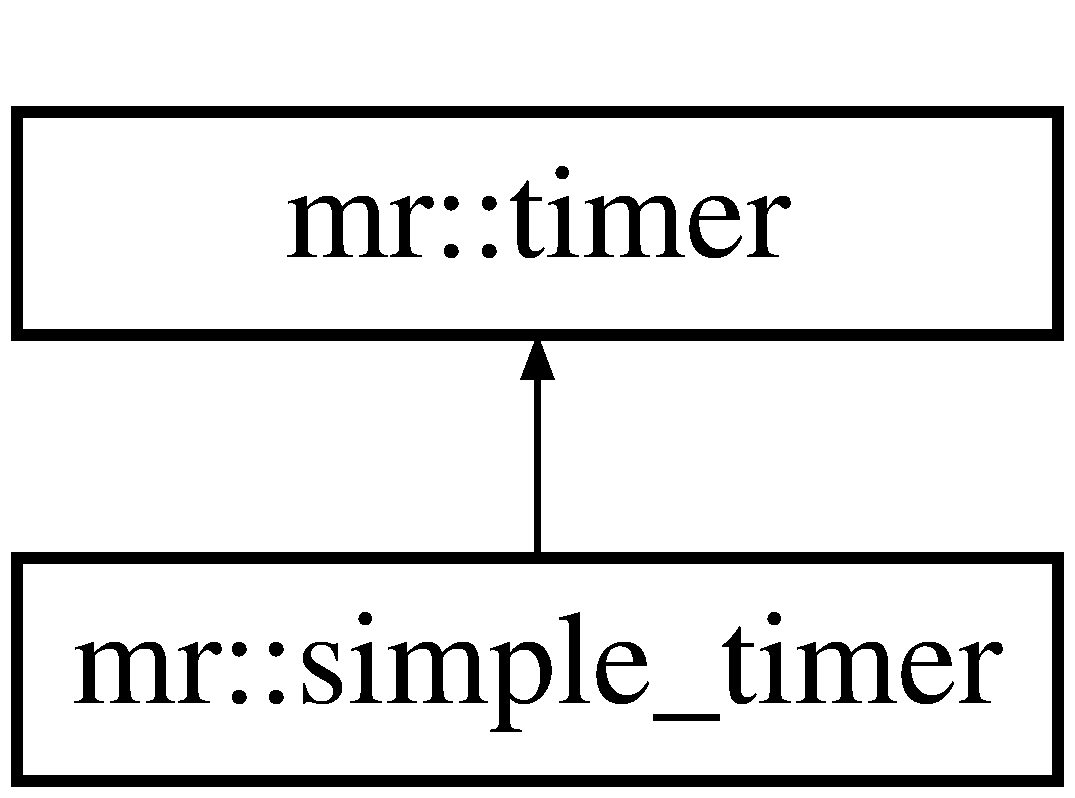
\includegraphics[height=2cm]{classmr_1_1timer}
\end{center}
\end{figure}
\subsection*{Public Member Functions}
\begin{CompactItemize}
\item 
{\bf timer} (mi\-Uint l=0)
\item 
{\bf timer} (const {\bf timer} \&b)
\item 
{\bf $\sim$timer} ()
\item 
void {\bf print} ()
\item 
void {\bf start} ()
\item 
void {\bf stop} ()
\item 
bool {\bf operator$>$} (const {\bf timer} \&b) const 
\item 
bool {\bf operator$<$} (const {\bf timer} \&b) const 
\item 
{\bf timer} \& {\bf operator+=} (const {\bf timer} \&b)
\item 
{\bf timer} \& {\bf operator-=} (const {\bf timer} \&b)
\end{CompactItemize}


\subsection{Detailed Description}
Very simple class/macro for profiling stuff... Just use it like:



\footnotesize\begin{verbatim}       mr::timer t1;
       // ... stuff to profile goes here...
       t1.stop();
   
       mr::timer t2;
       // ... stuff to profile goes here...
       t2.stop();
   
       if ( t1 < t2 ) mi_info("t1 is faster");
       else mi_info("t2 is faster");
\end{verbatim}
\normalsize




\subsection{Constructor \& Destructor Documentation}
\index{mr::timer@{mr::timer}!timer@{timer}}
\index{timer@{timer}!mr::timer@{mr::timer}}
\subsubsection{\setlength{\rightskip}{0pt plus 5cm}mr::timer::timer (mi\-Uint {\em l} = 0)\hspace{0.3cm}{\tt  [inline]}}\label{classmr_1_1timer_a0}


\index{mr::timer@{mr::timer}!timer@{timer}}
\index{timer@{timer}!mr::timer@{mr::timer}}
\subsubsection{\setlength{\rightskip}{0pt plus 5cm}mr::timer::timer (const {\bf timer} \& {\em b})\hspace{0.3cm}{\tt  [inline]}}\label{classmr_1_1timer_a1}


\index{mr::timer@{mr::timer}!~timer@{$\sim$timer}}
\index{~timer@{$\sim$timer}!mr::timer@{mr::timer}}
\subsubsection{\setlength{\rightskip}{0pt plus 5cm}mr::timer::$\sim${\bf timer} ()\hspace{0.3cm}{\tt  [inline]}}\label{classmr_1_1timer_a2}




\subsection{Member Function Documentation}
\index{mr::timer@{mr::timer}!operator+=@{operator+=}}
\index{operator+=@{operator+=}!mr::timer@{mr::timer}}
\subsubsection{\setlength{\rightskip}{0pt plus 5cm}{\bf timer}\& mr::timer::operator+= (const {\bf timer} \& {\em b})\hspace{0.3cm}{\tt  [inline]}}\label{classmr_1_1timer_a8}


\index{mr::timer@{mr::timer}!operator-=@{operator-=}}
\index{operator-=@{operator-=}!mr::timer@{mr::timer}}
\subsubsection{\setlength{\rightskip}{0pt plus 5cm}{\bf timer}\& mr::timer::operator-= (const {\bf timer} \& {\em b})\hspace{0.3cm}{\tt  [inline]}}\label{classmr_1_1timer_a9}


\index{mr::timer@{mr::timer}!operator<@{operator$<$}}
\index{operator<@{operator$<$}!mr::timer@{mr::timer}}
\subsubsection{\setlength{\rightskip}{0pt plus 5cm}bool mr::timer::operator$<$ (const {\bf timer} \& {\em b}) const\hspace{0.3cm}{\tt  [inline]}}\label{classmr_1_1timer_a7}


\index{mr::timer@{mr::timer}!operator>@{operator$>$}}
\index{operator>@{operator$>$}!mr::timer@{mr::timer}}
\subsubsection{\setlength{\rightskip}{0pt plus 5cm}bool mr::timer::operator$>$ (const {\bf timer} \& {\em b}) const\hspace{0.3cm}{\tt  [inline]}}\label{classmr_1_1timer_a6}


\index{mr::timer@{mr::timer}!print@{print}}
\index{print@{print}!mr::timer@{mr::timer}}
\subsubsection{\setlength{\rightskip}{0pt plus 5cm}void mr::timer::print ()\hspace{0.3cm}{\tt  [inline]}}\label{classmr_1_1timer_a3}


\index{mr::timer@{mr::timer}!start@{start}}
\index{start@{start}!mr::timer@{mr::timer}}
\subsubsection{\setlength{\rightskip}{0pt plus 5cm}void mr::timer::start ()\hspace{0.3cm}{\tt  [inline]}}\label{classmr_1_1timer_a4}


\index{mr::timer@{mr::timer}!stop@{stop}}
\index{stop@{stop}!mr::timer@{mr::timer}}
\subsubsection{\setlength{\rightskip}{0pt plus 5cm}void mr::timer::stop ()\hspace{0.3cm}{\tt  [inline]}}\label{classmr_1_1timer_a5}




The documentation for this class was generated from the following file:\begin{CompactItemize}
\item 
{\bf mr\-Profile.h}\end{CompactItemize}

\section{mr::Triangle\-Vertex\-Cache Class Reference}
\label{classmr_1_1TriangleVertexCache}\index{mr::TriangleVertexCache@{mr::TriangleVertexCache}}
{\tt \#include $<$mr\-Cache.h$>$}

\subsection*{Public Member Functions}
\begin{CompactItemize}
\item 
{\bf Triangle\-Vertex\-Cache} ()
\item 
{\bf $\sim$Triangle\-Vertex\-Cache} ()
\item 
void {\bf lock} ()
\item 
void {\bf unlock} ()
\item 
void {\bf reflection} (const mi\-State $\ast$const state, const mi\-Uint samples, const mi\-Scalar cos\-Angle=0.1f)
\item 
void {\bf refraction} (const mi\-State $\ast$const state, const mi\-Uint samples, const mi\-Scalar cos\-Angle=0.1f)
\item 
{\bf color} {\bf interpolate} (const mi\-State $\ast$const state)
\end{CompactItemize}


\subsection{Detailed Description}
This class is used as a cache for colors in vertices . It can be used for 'pre-baking' stuff. This class is still experimental (ie. does not work that well).

Usage is...



\footnotesize\begin{verbatim}     EXTERN_C DLLEXPORT void
     gg_phong_init(
              miState* const        state,
              struct gg_phong_t* p,
              miBoolean* req_inst
              )
     {
       if ( !p ) {  
         *req_inst = miTRUE; return;
       }
   
       TriangleVertexCache* cache = new TriangleVertexCache;
       void **user;
       mi_query(miQ_FUNC_USERPTR, state, 0, &user);
       *user = cache;
   
     }
   
   
     EXTERN_C DLLEXPORT void
     gg_phong_exit(
              miState* const        state,
              struct gg_ambientocclusion_t* p
              )
     {
       if ( !p ) return;
   
       void **user;
       mi_query(miQ_FUNC_USERPTR, state, 0, &user);
       delete *user;
     }
   
   
     EXTERN_C DLLEXPORT miBoolean 
     gg_phong(
         color* const result,
         miState* const state,
         struct gg_phong_t* p
         )
     {
       void **user;
       mi_query(miQ_FUNC_USERPTR, state, 0, &user);
       TriangleVertexCache* cache = static_cast< TriangleVertexCache* >(*user);
   
       cache->lock();
       cache->reflection( state, 16, 1 );
       *result = cache->interpolate( state );
       cache->unlock();
   
       return(miTRUE);
     }
\end{verbatim}
\normalsize




\subsection{Constructor \& Destructor Documentation}
\index{mr::TriangleVertexCache@{mr::Triangle\-Vertex\-Cache}!TriangleVertexCache@{TriangleVertexCache}}
\index{TriangleVertexCache@{TriangleVertexCache}!mr::TriangleVertexCache@{mr::Triangle\-Vertex\-Cache}}
\subsubsection{\setlength{\rightskip}{0pt plus 5cm}mr::Triangle\-Vertex\-Cache::Triangle\-Vertex\-Cache ()\hspace{0.3cm}{\tt  [inline]}}\label{classmr_1_1TriangleVertexCache_a0}


\index{mr::TriangleVertexCache@{mr::Triangle\-Vertex\-Cache}!~TriangleVertexCache@{$\sim$TriangleVertexCache}}
\index{~TriangleVertexCache@{$\sim$TriangleVertexCache}!mr::TriangleVertexCache@{mr::Triangle\-Vertex\-Cache}}
\subsubsection{\setlength{\rightskip}{0pt plus 5cm}mr::Triangle\-Vertex\-Cache::$\sim${\bf Triangle\-Vertex\-Cache} ()\hspace{0.3cm}{\tt  [inline]}}\label{classmr_1_1TriangleVertexCache_a1}




\subsection{Member Function Documentation}
\index{mr::TriangleVertexCache@{mr::Triangle\-Vertex\-Cache}!interpolate@{interpolate}}
\index{interpolate@{interpolate}!mr::TriangleVertexCache@{mr::Triangle\-Vertex\-Cache}}
\subsubsection{\setlength{\rightskip}{0pt plus 5cm}{\bf color} mr::Triangle\-Vertex\-Cache::interpolate (const mi\-State $\ast$const {\em state})\hspace{0.3cm}{\tt  [inline]}}\label{classmr_1_1TriangleVertexCache_a6}


\index{mr::TriangleVertexCache@{mr::Triangle\-Vertex\-Cache}!lock@{lock}}
\index{lock@{lock}!mr::TriangleVertexCache@{mr::Triangle\-Vertex\-Cache}}
\subsubsection{\setlength{\rightskip}{0pt plus 5cm}void mr::Triangle\-Vertex\-Cache::lock ()\hspace{0.3cm}{\tt  [inline]}}\label{classmr_1_1TriangleVertexCache_a2}


\index{mr::TriangleVertexCache@{mr::Triangle\-Vertex\-Cache}!reflection@{reflection}}
\index{reflection@{reflection}!mr::TriangleVertexCache@{mr::Triangle\-Vertex\-Cache}}
\subsubsection{\setlength{\rightskip}{0pt plus 5cm}void mr::Triangle\-Vertex\-Cache::reflection (const mi\-State $\ast$const {\em state}, const mi\-Uint {\em samples}, const mi\-Scalar {\em cos\-Angle} = 0.1f)\hspace{0.3cm}{\tt  [inline]}}\label{classmr_1_1TriangleVertexCache_a4}


\index{mr::TriangleVertexCache@{mr::Triangle\-Vertex\-Cache}!refraction@{refraction}}
\index{refraction@{refraction}!mr::TriangleVertexCache@{mr::Triangle\-Vertex\-Cache}}
\subsubsection{\setlength{\rightskip}{0pt plus 5cm}void mr::Triangle\-Vertex\-Cache::refraction (const mi\-State $\ast$const {\em state}, const mi\-Uint {\em samples}, const mi\-Scalar {\em cos\-Angle} = 0.1f)\hspace{0.3cm}{\tt  [inline]}}\label{classmr_1_1TriangleVertexCache_a5}


\index{mr::TriangleVertexCache@{mr::Triangle\-Vertex\-Cache}!unlock@{unlock}}
\index{unlock@{unlock}!mr::TriangleVertexCache@{mr::Triangle\-Vertex\-Cache}}
\subsubsection{\setlength{\rightskip}{0pt plus 5cm}void mr::Triangle\-Vertex\-Cache::unlock ()\hspace{0.3cm}{\tt  [inline]}}\label{classmr_1_1TriangleVertexCache_a3}




The documentation for this class was generated from the following file:\begin{CompactItemize}
\item 
{\bf mr\-Cache.h}\end{CompactItemize}

\section{mr::tri\-Id Struct Reference}
\label{structmr_1_1triId}\index{mr::triId@{mr::triId}}
Identifies a triangle, as in mi\-State, but smaller.  


{\tt \#include $<$mr\-Functors.h$>$}

\subsection*{Public Attributes}
\begin{CompactItemize}
\item 
void $\ast$ {\bf pri}
\item 
int {\bf pri\_\-idx}
\end{CompactItemize}


\subsection{Detailed Description}
Identifies a triangle, as in mi\-State, but smaller. 



\subsection{Member Data Documentation}
\index{mr::triId@{mr::tri\-Id}!pri@{pri}}
\index{pri@{pri}!mr::triId@{mr::tri\-Id}}
\subsubsection{\setlength{\rightskip}{0pt plus 5cm}void$\ast$ {\bf mr::tri\-Id::pri}}\label{structmr_1_1triId_o0}


\index{mr::triId@{mr::tri\-Id}!pri_idx@{pri\_\-idx}}
\index{pri_idx@{pri\_\-idx}!mr::triId@{mr::tri\-Id}}
\subsubsection{\setlength{\rightskip}{0pt plus 5cm}int {\bf mr::tri\-Id::pri\_\-idx}}\label{structmr_1_1triId_o1}




The documentation for this struct was generated from the following file:\begin{CompactItemize}
\item 
{\bf mr\-Functors.h}\end{CompactItemize}

\section{mr::distances::Type Struct Reference}
\label{structmr_1_1distances_1_1Type}\index{mr::distances::Type@{mr::distances::Type}}
{\tt \#include $<$mr\-Distances.h$>$}

Inheritance diagram for mr::distances::Type::\begin{figure}[H]
\begin{center}
\leavevmode
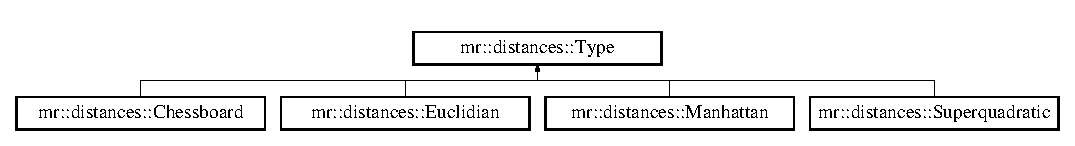
\includegraphics[height=1.51351cm]{structmr_1_1distances_1_1Type}
\end{center}
\end{figure}
\subsection*{Public Member Functions}
\begin{CompactItemize}
\item 
virtual mi\-Scalar {\bf operator()} (const {\bf vector} \&d) const=0
\item 
virtual mi\-Scalar {\bf operator()} (const {\bf vector} \&d, const {\bf vector} \&s) const=0
\end{CompactItemize}


\subsection{Detailed Description}
Different functors that can be used to measure common distance measurements. 



\subsection{Member Function Documentation}
\index{mr::distances::Type@{mr::distances::Type}!operator()@{operator()}}
\index{operator()@{operator()}!mr::distances::Type@{mr::distances::Type}}
\subsubsection{\setlength{\rightskip}{0pt plus 5cm}virtual mi\-Scalar mr::distances::Type::operator() (const {\bf vector} \& {\em d}, const {\bf vector} \& {\em s}) const\hspace{0.3cm}{\tt  [pure virtual]}}\label{structmr_1_1distances_1_1Type_a1}




Implemented in {\bf mr::distances::Euclidian} {\rm (p.\,\pageref{structmr_1_1distances_1_1Euclidian_a1})}, {\bf mr::distances::Manhattan} {\rm (p.\,\pageref{structmr_1_1distances_1_1Manhattan_a1})}, {\bf mr::distances::Chessboard} {\rm (p.\,\pageref{structmr_1_1distances_1_1Chessboard_a1})}, and {\bf mr::distances::Superquadratic} {\rm (p.\,\pageref{structmr_1_1distances_1_1Superquadratic_a1})}.\index{mr::distances::Type@{mr::distances::Type}!operator()@{operator()}}
\index{operator()@{operator()}!mr::distances::Type@{mr::distances::Type}}
\subsubsection{\setlength{\rightskip}{0pt plus 5cm}virtual mi\-Scalar mr::distances::Type::operator() (const {\bf vector} \& {\em d}) const\hspace{0.3cm}{\tt  [pure virtual]}}\label{structmr_1_1distances_1_1Type_a0}




Implemented in {\bf mr::distances::Euclidian} {\rm (p.\,\pageref{structmr_1_1distances_1_1Euclidian_a0})}, {\bf mr::distances::Manhattan} {\rm (p.\,\pageref{structmr_1_1distances_1_1Manhattan_a0})}, {\bf mr::distances::Chessboard} {\rm (p.\,\pageref{structmr_1_1distances_1_1Chessboard_a0})}, and {\bf mr::distances::Superquadratic} {\rm (p.\,\pageref{structmr_1_1distances_1_1Superquadratic_a0})}.

The documentation for this struct was generated from the following file:\begin{CompactItemize}
\item 
{\bf mr\-Distances.h}\end{CompactItemize}

\section{mr::UVCache Class Reference}
\label{classmr_1_1UVCache}\index{mr::UVCache@{mr::UVCache}}
{\tt \#include $<$mr\-Cache.h$>$}

\subsection*{Public Member Functions}
\begin{CompactItemize}
\item 
{\bf UVCache} (const mi\-Uint xres, const mi\-Uint yres)
\item 
{\bf $\sim$UVCache} ()
\item 
void {\bf lock} ()
\item 
void {\bf unlock} ()
\item 
void {\bf reflection} (mi\-State $\ast$const state, const mi\-Uint num\-Samples, const mi\-Scalar cosine=0.1f)
\item 
void {\bf refraction} (const mi\-State $\ast$const state, const mi\-Uint num\-Samples, const mi\-Scalar cosine=0.1f)
\item 
{\bf color} {\bf interpolate} (mi\-State $\ast$const state)
\end{CompactItemize}


\subsection{Detailed Description}
This class is used as a cache for colors based on UVs. It can be used for 'pre-baking' stuff, similar to {\bf Triangle\-Vertex\-Cache}{\rm (p.\,\pageref{classmr_1_1TriangleVertexCache})}. This class is still experimental (ie. does not work that well). 



\subsection{Constructor \& Destructor Documentation}
\index{mr::UVCache@{mr::UVCache}!UVCache@{UVCache}}
\index{UVCache@{UVCache}!mr::UVCache@{mr::UVCache}}
\subsubsection{\setlength{\rightskip}{0pt plus 5cm}mr::UVCache::UVCache (const mi\-Uint {\em xres}, const mi\-Uint {\em yres})\hspace{0.3cm}{\tt  [inline]}}\label{classmr_1_1UVCache_a0}


\index{mr::UVCache@{mr::UVCache}!~UVCache@{$\sim$UVCache}}
\index{~UVCache@{$\sim$UVCache}!mr::UVCache@{mr::UVCache}}
\subsubsection{\setlength{\rightskip}{0pt plus 5cm}mr::UVCache::$\sim${\bf UVCache} ()\hspace{0.3cm}{\tt  [inline]}}\label{classmr_1_1UVCache_a1}




\subsection{Member Function Documentation}
\index{mr::UVCache@{mr::UVCache}!interpolate@{interpolate}}
\index{interpolate@{interpolate}!mr::UVCache@{mr::UVCache}}
\subsubsection{\setlength{\rightskip}{0pt plus 5cm}{\bf color} mr::UVCache::interpolate (mi\-State $\ast$const {\em state})\hspace{0.3cm}{\tt  [inline]}}\label{classmr_1_1UVCache_a6}


\index{mr::UVCache@{mr::UVCache}!lock@{lock}}
\index{lock@{lock}!mr::UVCache@{mr::UVCache}}
\subsubsection{\setlength{\rightskip}{0pt plus 5cm}void mr::UVCache::lock ()\hspace{0.3cm}{\tt  [inline]}}\label{classmr_1_1UVCache_a2}


\index{mr::UVCache@{mr::UVCache}!reflection@{reflection}}
\index{reflection@{reflection}!mr::UVCache@{mr::UVCache}}
\subsubsection{\setlength{\rightskip}{0pt plus 5cm}void mr::UVCache::reflection (mi\-State $\ast$const {\em state}, const mi\-Uint {\em num\-Samples}, const mi\-Scalar {\em cosine} = 0.1f)\hspace{0.3cm}{\tt  [inline]}}\label{classmr_1_1UVCache_a4}


\index{mr::UVCache@{mr::UVCache}!refraction@{refraction}}
\index{refraction@{refraction}!mr::UVCache@{mr::UVCache}}
\subsubsection{\setlength{\rightskip}{0pt plus 5cm}void mr::UVCache::refraction (const mi\-State $\ast$const {\em state}, const mi\-Uint {\em num\-Samples}, const mi\-Scalar {\em cosine} = 0.1f)\hspace{0.3cm}{\tt  [inline]}}\label{classmr_1_1UVCache_a5}


\index{mr::UVCache@{mr::UVCache}!unlock@{unlock}}
\index{unlock@{unlock}!mr::UVCache@{mr::UVCache}}
\subsubsection{\setlength{\rightskip}{0pt plus 5cm}void mr::UVCache::unlock ()\hspace{0.3cm}{\tt  [inline]}}\label{classmr_1_1UVCache_a3}




The documentation for this class was generated from the following file:\begin{CompactItemize}
\item 
{\bf mr\-Cache.h}\end{CompactItemize}

\section{mr::VCell Class Reference}
\label{classmr_1_1VCell}\index{mr::VCell@{mr::VCell}}
Cellnoise class returning a vector.  


{\tt \#include $<$mr\-Cell.h$>$}

\subsection*{Static Public Member Functions}
\begin{CompactItemize}
\item 
{\bf vector} {\bf noise} (mi\-Scalar x)
\item 
{\bf vector} {\bf noise} (mi\-Scalar x, mi\-Scalar y)
\item 
{\bf vector} {\bf noise} (mi\-Scalar x, mi\-Scalar y, mi\-Scalar z)
\item 
{\bf vector} {\bf noise} (mi\-Scalar x, mi\-Scalar y, mi\-Scalar z, mi\-Scalar t)
\item 
{\bf vector} {\bf noise} (const {\bf vector2d} \&P)
\item 
{\bf vector} {\bf noise} (const {\bf point} \&P)
\item 
{\bf vector} {\bf noise} (const {\bf point} \&P, const mi\-Scalar t)
\end{CompactItemize}


\subsection{Detailed Description}
Cellnoise class returning a vector. 



\subsection{Member Function Documentation}
\index{mr::VCell@{mr::VCell}!noise@{noise}}
\index{noise@{noise}!mr::VCell@{mr::VCell}}
\subsubsection{\setlength{\rightskip}{0pt plus 5cm}{\bf vector} mr::VCell::noise (const {\bf point} \& {\em P}, const mi\-Scalar {\em t})\hspace{0.3cm}{\tt  [inline, static]}}\label{classmr_1_1VCell_e6}


\index{mr::VCell@{mr::VCell}!noise@{noise}}
\index{noise@{noise}!mr::VCell@{mr::VCell}}
\subsubsection{\setlength{\rightskip}{0pt plus 5cm}{\bf vector} mr::VCell::noise (const {\bf point} \& {\em P})\hspace{0.3cm}{\tt  [inline, static]}}\label{classmr_1_1VCell_e5}


\index{mr::VCell@{mr::VCell}!noise@{noise}}
\index{noise@{noise}!mr::VCell@{mr::VCell}}
\subsubsection{\setlength{\rightskip}{0pt plus 5cm}{\bf vector} mr::VCell::noise (const {\bf vector2d} \& {\em P})\hspace{0.3cm}{\tt  [inline, static]}}\label{classmr_1_1VCell_e4}


\index{mr::VCell@{mr::VCell}!noise@{noise}}
\index{noise@{noise}!mr::VCell@{mr::VCell}}
\subsubsection{\setlength{\rightskip}{0pt plus 5cm}{\bf vector} mr::VCell::noise (mi\-Scalar {\em x}, mi\-Scalar {\em y}, mi\-Scalar {\em z}, mi\-Scalar {\em t})\hspace{0.3cm}{\tt  [inline, static]}}\label{classmr_1_1VCell_e3}


\index{mr::VCell@{mr::VCell}!noise@{noise}}
\index{noise@{noise}!mr::VCell@{mr::VCell}}
\subsubsection{\setlength{\rightskip}{0pt plus 5cm}{\bf vector} mr::VCell::noise (mi\-Scalar {\em x}, mi\-Scalar {\em y}, mi\-Scalar {\em z})\hspace{0.3cm}{\tt  [inline, static]}}\label{classmr_1_1VCell_e2}


\index{mr::VCell@{mr::VCell}!noise@{noise}}
\index{noise@{noise}!mr::VCell@{mr::VCell}}
\subsubsection{\setlength{\rightskip}{0pt plus 5cm}{\bf vector} mr::VCell::noise (mi\-Scalar {\em x}, mi\-Scalar {\em y})\hspace{0.3cm}{\tt  [inline, static]}}\label{classmr_1_1VCell_e1}


\index{mr::VCell@{mr::VCell}!noise@{noise}}
\index{noise@{noise}!mr::VCell@{mr::VCell}}
\subsubsection{\setlength{\rightskip}{0pt plus 5cm}{\bf vector} mr::VCell::noise (mi\-Scalar {\em x})\hspace{0.3cm}{\tt  [inline, static]}}\label{classmr_1_1VCell_e0}




The documentation for this class was generated from the following file:\begin{CompactItemize}
\item 
{\bf mr\-Cell.h}\end{CompactItemize}

\section{mr::base::vec2 Struct Reference}
\label{structmr_1_1base_1_1vec2}\index{mr::base::vec2@{mr::base::vec2}}
{\tt \#include $<$mr\-Vector.h$>$}

\subsection*{Public Types}
\begin{CompactItemize}
\item 
typedef mi\-Vector2d {\bf C}
\item 
typedef {\bf vec2} {\bf self}
\item 
typedef mi\-Scalar {\bf T}
\end{CompactItemize}
\subsection*{Public Member Functions}
\begin{CompactItemize}
\item 
const mi\-Scalar {\bf Evaluate} (const unsigned short i) const 
\item 
{\bf self} {\bf less\-Than} (const mi\-Vector2d \&b)
\item 
{\bf self} {\bf less\-Than\-Equal} (const mi\-Vector2d \&b)
\item 
{\bf self} {\bf greater\-Than} (const mi\-Vector2d \&b)
\item 
{\bf self} {\bf greater\-Than\-Equal} (const mi\-Vector2d \&b)
\item 
bool {\bf any} ()
\item 
const bool {\bf is\-Equivalent} (const mi\-Vector2d \&b, const mi\-Scalar tolerance=mi\-SCALAR\_\-EPSILON) const 
\item 
const {\bf self} \& {\bf mix} (const mi\-Vector2d \&b, const mi\-Scalar p)
\item 
const {\bf self} \& {\bf uv} () const 
\item 
{\bf self} {\bf vu} () const 
\item 
{\bf self} {\bf uu} () const 
\item 
{\bf self} {\bf vv} () const 
\end{CompactItemize}
\begin{Indent}{\bf Constructors}\par
\begin{CompactItemize}
\item 
{\bf vec2} ({\bf k\-No\-Construct})
\begin{CompactList}\small\item\em Constructor that does nothing (fast). Use as vector2d x(k\-No\-Init). \item\end{CompactList}\item 
{\bf vec2} ()
\begin{CompactList}\small\item\em Constructor that initializes vector to 0. \item\end{CompactList}\item 
{\bf vec2} (const mi\-Scalar uu, const mi\-Scalar vv)
\begin{CompactList}\small\item\em Constructor that initializes it from two mi\-Scalars. \item\end{CompactList}\item 
{\bf vec2} (const mi\-Vector2d \&b)
\begin{CompactList}\small\item\em Constructor from an mi\-Vector2d. \item\end{CompactList}\item 
template$<$class X, class Y, class Oper$>$ {\bf vec2} (const {\bf base::exp}$<$ X, Y, Oper $>$ \&e)
\begin{CompactList}\small\item\em Constructor from an expression. \item\end{CompactList}\end{CompactItemize}
\end{Indent}
\begin{Indent}{\bf Copy Constructor}\par
\begin{CompactItemize}
\item 
{\bf vec2} (const {\bf vec2} \&b)
\end{CompactItemize}
\end{Indent}
\begin{Indent}{\bf Accessors}\par
\begin{CompactItemize}
\item 
{\bf T} \& {\bf operator[$\,$]} (const unsigned short i)
\begin{CompactList}\small\item\em Allow access to each element of vector for assignment. \item\end{CompactList}\item 
const {\bf T} {\bf operator[$\,$]} (const unsigned short i) const 
\begin{CompactList}\small\item\em Allow access to each element of vector for reading. \item\end{CompactList}\item 
void {\bf set} (const unsigned short i, const {\bf T} t)
\begin{CompactList}\small\item\em Allow assignment to an element of a vector. \item\end{CompactList}\item 
void {\bf set} (const {\bf T} uu, const {\bf T} vv)
\begin{CompactList}\small\item\em Allow assignment to an elements of a vector. \item\end{CompactList}\item 
const {\bf T} {\bf get} (const unsigned short i) const 
\begin{CompactList}\small\item\em Allow access to an element of vector for reading. \item\end{CompactList}\end{CompactItemize}
\end{Indent}
\begin{Indent}{\bf Assignment}\par
\begin{CompactItemize}
\item 
template$<$class X, class Y, class Oper$>$ const {\bf self} \& {\bf operator=} (const {\bf base::exp}$<$ X, Y, Oper $>$ \&e)
\item 
const {\bf self} \& {\bf operator=} (const {\bf self} \&b)
\item 
const {\bf self} \& {\bf operator=} (const mi\-Vector2d \&b)
\item 
const {\bf self} \& {\bf operator=} (const mi\-Scalar b)
\end{CompactItemize}
\end{Indent}
\begin{Indent}{\bf Equality}\par
\begin{CompactItemize}
\item 
template$<$class X, class Y, class Oper$>$ const bool {\bf operator==} (const {\bf base::exp}$<$ X, Y, Oper $>$ \&x) const 
\item 
const bool {\bf operator==} (const {\bf self} \&b) const 
\item 
const bool {\bf operator==} (const mi\-Vector2d \&b) const 
\item 
const bool {\bf operator==} (const mi\-Scalar b) const 
\item 
template$<$class X, class Y, class Oper$>$ const bool {\bf operator!=} (const {\bf base::exp}$<$ X, Y, Oper $>$ \&b) const 
\item 
const bool {\bf operator!=} (const {\bf self} \&b) const 
\item 
const bool {\bf operator!=} (const mi\-Vector2d \&b) const 
\item 
const bool {\bf operator!=} (const mi\-Scalar b) const 
\end{CompactItemize}
\end{Indent}
\begin{Indent}{\bf REFERENCE OPERATORS (MODIFY IN PLACE)}\par
\begin{CompactItemize}
\item 
template$<$class X, class Y, class Oper$>$ const {\bf self} \& {\bf operator+=} (const {\bf base::exp}$<$ X, Y, Oper $>$ \&b)
\item 
const {\bf self} \& {\bf operator+=} (const mi\-Scalar b)
\item 
const {\bf self} \& {\bf operator+=} (const mi\-Vector2d \&b)
\item 
template$<$class X, class Y, class Oper$>$ const {\bf self} \& {\bf operator-=} (const {\bf base::exp}$<$ X, Y, Oper $>$ \&b)
\item 
const {\bf self} \& {\bf operator-=} (const mi\-Scalar b)
\item 
const {\bf self} \& {\bf operator-=} (const mi\-Vector2d \&b)
\item 
template$<$class X, class Y, class Oper$>$ const {\bf self} \& {\bf operator $\ast$=} (const {\bf base::exp}$<$ X, Y, Oper $>$ \&b)
\item 
const {\bf self} \& {\bf operator $\ast$=} (const mi\-Scalar b)
\item 
const {\bf self} \& {\bf operator $\ast$=} (const mi\-Vector2d \&b)
\item 
template$<$class X, class Y, class Oper$>$ const {\bf self} \& {\bf operator/=} (const {\bf base::exp}$<$ X, Y, Oper $>$ \&b)
\item 
const {\bf self} \& {\bf operator/=} (const mi\-Scalar b)
\item 
const {\bf self} \& {\bf operator/=} (const mi\-Vector2d \&b)
\end{CompactItemize}
\end{Indent}


\subsection{Member Typedef Documentation}
\index{mr::base::vec2@{mr::base::vec2}!C@{C}}
\index{C@{C}!mr::base::vec2@{mr::base::vec2}}
\subsubsection{\setlength{\rightskip}{0pt plus 5cm}typedef mi\-Vector2d {\bf mr::base::vec2::C}}\label{structmr_1_1base_1_1vec2_w0}


\index{mr::base::vec2@{mr::base::vec2}!self@{self}}
\index{self@{self}!mr::base::vec2@{mr::base::vec2}}
\subsubsection{\setlength{\rightskip}{0pt plus 5cm}typedef {\bf vec2} {\bf mr::base::vec2::self}}\label{structmr_1_1base_1_1vec2_w1}


\index{mr::base::vec2@{mr::base::vec2}!T@{T}}
\index{T@{T}!mr::base::vec2@{mr::base::vec2}}
\subsubsection{\setlength{\rightskip}{0pt plus 5cm}typedef mi\-Scalar {\bf mr::base::vec2::T}}\label{structmr_1_1base_1_1vec2_w2}




\subsection{Constructor \& Destructor Documentation}
\index{mr::base::vec2@{mr::base::vec2}!vec2@{vec2}}
\index{vec2@{vec2}!mr::base::vec2@{mr::base::vec2}}
\subsubsection{\setlength{\rightskip}{0pt plus 5cm}mr::base::vec2::vec2 ({\bf k\-No\-Construct})\hspace{0.3cm}{\tt  [inline]}}\label{structmr_1_1base_1_1vec2_z45_0}


Constructor that does nothing (fast). Use as vector2d x(k\-No\-Init). 

\index{mr::base::vec2@{mr::base::vec2}!vec2@{vec2}}
\index{vec2@{vec2}!mr::base::vec2@{mr::base::vec2}}
\subsubsection{\setlength{\rightskip}{0pt plus 5cm}mr::base::vec2::vec2 ()\hspace{0.3cm}{\tt  [inline]}}\label{structmr_1_1base_1_1vec2_z45_1}


Constructor that initializes vector to 0. 

\index{mr::base::vec2@{mr::base::vec2}!vec2@{vec2}}
\index{vec2@{vec2}!mr::base::vec2@{mr::base::vec2}}
\subsubsection{\setlength{\rightskip}{0pt plus 5cm}mr::base::vec2::vec2 (const mi\-Scalar {\em uu}, const mi\-Scalar {\em vv})\hspace{0.3cm}{\tt  [inline]}}\label{structmr_1_1base_1_1vec2_z45_2}


Constructor that initializes it from two mi\-Scalars. 

\index{mr::base::vec2@{mr::base::vec2}!vec2@{vec2}}
\index{vec2@{vec2}!mr::base::vec2@{mr::base::vec2}}
\subsubsection{\setlength{\rightskip}{0pt plus 5cm}mr::base::vec2::vec2 (const mi\-Vector2d \& {\em b})\hspace{0.3cm}{\tt  [inline]}}\label{structmr_1_1base_1_1vec2_z45_3}


Constructor from an mi\-Vector2d. 

\index{mr::base::vec2@{mr::base::vec2}!vec2@{vec2}}
\index{vec2@{vec2}!mr::base::vec2@{mr::base::vec2}}
\subsubsection{\setlength{\rightskip}{0pt plus 5cm}template$<$class X, class Y, class Oper$>$ mr::base::vec2::vec2 (const {\bf base::exp}$<$ X, Y, Oper $>$ \& {\em e})\hspace{0.3cm}{\tt  [inline]}}\label{structmr_1_1base_1_1vec2_z45_4}


Constructor from an expression. 

\index{mr::base::vec2@{mr::base::vec2}!vec2@{vec2}}
\index{vec2@{vec2}!mr::base::vec2@{mr::base::vec2}}
\subsubsection{\setlength{\rightskip}{0pt plus 5cm}mr::base::vec2::vec2 (const {\bf vec2} \& {\em b})\hspace{0.3cm}{\tt  [inline]}}\label{structmr_1_1base_1_1vec2_z46_0}




\subsection{Member Function Documentation}
\index{mr::base::vec2@{mr::base::vec2}!any@{any}}
\index{any@{any}!mr::base::vec2@{mr::base::vec2}}
\subsubsection{\setlength{\rightskip}{0pt plus 5cm}bool mr::base::vec2::any ()\hspace{0.3cm}{\tt  [inline]}}\label{structmr_1_1base_1_1vec2_a5}


\index{mr::base::vec2@{mr::base::vec2}!Evaluate@{Evaluate}}
\index{Evaluate@{Evaluate}!mr::base::vec2@{mr::base::vec2}}
\subsubsection{\setlength{\rightskip}{0pt plus 5cm}const mi\-Scalar mr::base::vec2::Evaluate (const unsigned short {\em i}) const\hspace{0.3cm}{\tt  [inline]}}\label{structmr_1_1base_1_1vec2_a0}


\index{mr::base::vec2@{mr::base::vec2}!get@{get}}
\index{get@{get}!mr::base::vec2@{mr::base::vec2}}
\subsubsection{\setlength{\rightskip}{0pt plus 5cm}const {\bf T} mr::base::vec2::get (const unsigned short {\em i}) const\hspace{0.3cm}{\tt  [inline]}}\label{structmr_1_1base_1_1vec2_z47_4}


Allow access to an element of vector for reading. 

\index{mr::base::vec2@{mr::base::vec2}!greaterThan@{greaterThan}}
\index{greaterThan@{greaterThan}!mr::base::vec2@{mr::base::vec2}}
\subsubsection{\setlength{\rightskip}{0pt plus 5cm}{\bf self} mr::base::vec2::greater\-Than (const mi\-Vector2d \& {\em b})\hspace{0.3cm}{\tt  [inline]}}\label{structmr_1_1base_1_1vec2_a3}


\index{mr::base::vec2@{mr::base::vec2}!greaterThanEqual@{greaterThanEqual}}
\index{greaterThanEqual@{greaterThanEqual}!mr::base::vec2@{mr::base::vec2}}
\subsubsection{\setlength{\rightskip}{0pt plus 5cm}{\bf self} mr::base::vec2::greater\-Than\-Equal (const mi\-Vector2d \& {\em b})\hspace{0.3cm}{\tt  [inline]}}\label{structmr_1_1base_1_1vec2_a4}


\index{mr::base::vec2@{mr::base::vec2}!isEquivalent@{isEquivalent}}
\index{isEquivalent@{isEquivalent}!mr::base::vec2@{mr::base::vec2}}
\subsubsection{\setlength{\rightskip}{0pt plus 5cm}const bool mr::base::vec2::is\-Equivalent (const mi\-Vector2d \& {\em b}, const mi\-Scalar {\em tolerance} = mi\-SCALAR\_\-EPSILON) const\hspace{0.3cm}{\tt  [inline]}}\label{structmr_1_1base_1_1vec2_a6}


\index{mr::base::vec2@{mr::base::vec2}!lessThan@{lessThan}}
\index{lessThan@{lessThan}!mr::base::vec2@{mr::base::vec2}}
\subsubsection{\setlength{\rightskip}{0pt plus 5cm}{\bf self} mr::base::vec2::less\-Than (const mi\-Vector2d \& {\em b})\hspace{0.3cm}{\tt  [inline]}}\label{structmr_1_1base_1_1vec2_a1}


\index{mr::base::vec2@{mr::base::vec2}!lessThanEqual@{lessThanEqual}}
\index{lessThanEqual@{lessThanEqual}!mr::base::vec2@{mr::base::vec2}}
\subsubsection{\setlength{\rightskip}{0pt plus 5cm}{\bf self} mr::base::vec2::less\-Than\-Equal (const mi\-Vector2d \& {\em b})\hspace{0.3cm}{\tt  [inline]}}\label{structmr_1_1base_1_1vec2_a2}


\index{mr::base::vec2@{mr::base::vec2}!mix@{mix}}
\index{mix@{mix}!mr::base::vec2@{mr::base::vec2}}
\subsubsection{\setlength{\rightskip}{0pt plus 5cm}const {\bf self}\& mr::base::vec2::mix (const mi\-Vector2d \& {\em b}, const mi\-Scalar {\em p})\hspace{0.3cm}{\tt  [inline]}}\label{structmr_1_1base_1_1vec2_a7}


\index{mr::base::vec2@{mr::base::vec2}!operator *=@{operator $\ast$=}}
\index{operator *=@{operator $\ast$=}!mr::base::vec2@{mr::base::vec2}}
\subsubsection{\setlength{\rightskip}{0pt plus 5cm}const {\bf self}\& mr::base::vec2::operator $\ast$= (const mi\-Vector2d \& {\em b})\hspace{0.3cm}{\tt  [inline]}}\label{structmr_1_1base_1_1vec2_z53_8}


\index{mr::base::vec2@{mr::base::vec2}!operator *=@{operator $\ast$=}}
\index{operator *=@{operator $\ast$=}!mr::base::vec2@{mr::base::vec2}}
\subsubsection{\setlength{\rightskip}{0pt plus 5cm}const {\bf self}\& mr::base::vec2::operator $\ast$= (const mi\-Scalar {\em b})\hspace{0.3cm}{\tt  [inline]}}\label{structmr_1_1base_1_1vec2_z53_7}


\index{mr::base::vec2@{mr::base::vec2}!operator *=@{operator $\ast$=}}
\index{operator *=@{operator $\ast$=}!mr::base::vec2@{mr::base::vec2}}
\subsubsection{\setlength{\rightskip}{0pt plus 5cm}template$<$class X, class Y, class Oper$>$ const {\bf self}\& mr::base::vec2::operator $\ast$= (const {\bf base::exp}$<$ X, Y, Oper $>$ \& {\em b})\hspace{0.3cm}{\tt  [inline]}}\label{structmr_1_1base_1_1vec2_z53_6}


\index{mr::base::vec2@{mr::base::vec2}!operator"!=@{operator"!=}}
\index{operator"!=@{operator"!=}!mr::base::vec2@{mr::base::vec2}}
\subsubsection{\setlength{\rightskip}{0pt plus 5cm}const bool mr::base::vec2::operator!= (const mi\-Scalar {\em b}) const\hspace{0.3cm}{\tt  [inline]}}\label{structmr_1_1base_1_1vec2_z51_7}


\index{mr::base::vec2@{mr::base::vec2}!operator"!=@{operator"!=}}
\index{operator"!=@{operator"!=}!mr::base::vec2@{mr::base::vec2}}
\subsubsection{\setlength{\rightskip}{0pt plus 5cm}const bool mr::base::vec2::operator!= (const mi\-Vector2d \& {\em b}) const\hspace{0.3cm}{\tt  [inline]}}\label{structmr_1_1base_1_1vec2_z51_6}


\index{mr::base::vec2@{mr::base::vec2}!operator"!=@{operator"!=}}
\index{operator"!=@{operator"!=}!mr::base::vec2@{mr::base::vec2}}
\subsubsection{\setlength{\rightskip}{0pt plus 5cm}const bool mr::base::vec2::operator!= (const {\bf self} \& {\em b}) const\hspace{0.3cm}{\tt  [inline]}}\label{structmr_1_1base_1_1vec2_z51_5}


\index{mr::base::vec2@{mr::base::vec2}!operator"!=@{operator"!=}}
\index{operator"!=@{operator"!=}!mr::base::vec2@{mr::base::vec2}}
\subsubsection{\setlength{\rightskip}{0pt plus 5cm}template$<$class X, class Y, class Oper$>$ const bool mr::base::vec2::operator!= (const {\bf base::exp}$<$ X, Y, Oper $>$ \& {\em b}) const\hspace{0.3cm}{\tt  [inline]}}\label{structmr_1_1base_1_1vec2_z51_4}


\index{mr::base::vec2@{mr::base::vec2}!operator+=@{operator+=}}
\index{operator+=@{operator+=}!mr::base::vec2@{mr::base::vec2}}
\subsubsection{\setlength{\rightskip}{0pt plus 5cm}const {\bf self}\& mr::base::vec2::operator+= (const mi\-Vector2d \& {\em b})\hspace{0.3cm}{\tt  [inline]}}\label{structmr_1_1base_1_1vec2_z53_2}


\index{mr::base::vec2@{mr::base::vec2}!operator+=@{operator+=}}
\index{operator+=@{operator+=}!mr::base::vec2@{mr::base::vec2}}
\subsubsection{\setlength{\rightskip}{0pt plus 5cm}const {\bf self}\& mr::base::vec2::operator+= (const mi\-Scalar {\em b})\hspace{0.3cm}{\tt  [inline]}}\label{structmr_1_1base_1_1vec2_z53_1}


\index{mr::base::vec2@{mr::base::vec2}!operator+=@{operator+=}}
\index{operator+=@{operator+=}!mr::base::vec2@{mr::base::vec2}}
\subsubsection{\setlength{\rightskip}{0pt plus 5cm}template$<$class X, class Y, class Oper$>$ const {\bf self}\& mr::base::vec2::operator+= (const {\bf base::exp}$<$ X, Y, Oper $>$ \& {\em b})\hspace{0.3cm}{\tt  [inline]}}\label{structmr_1_1base_1_1vec2_z53_0}


\index{mr::base::vec2@{mr::base::vec2}!operator-=@{operator-=}}
\index{operator-=@{operator-=}!mr::base::vec2@{mr::base::vec2}}
\subsubsection{\setlength{\rightskip}{0pt plus 5cm}const {\bf self}\& mr::base::vec2::operator-= (const mi\-Vector2d \& {\em b})\hspace{0.3cm}{\tt  [inline]}}\label{structmr_1_1base_1_1vec2_z53_5}


\index{mr::base::vec2@{mr::base::vec2}!operator-=@{operator-=}}
\index{operator-=@{operator-=}!mr::base::vec2@{mr::base::vec2}}
\subsubsection{\setlength{\rightskip}{0pt plus 5cm}const {\bf self}\& mr::base::vec2::operator-= (const mi\-Scalar {\em b})\hspace{0.3cm}{\tt  [inline]}}\label{structmr_1_1base_1_1vec2_z53_4}


\index{mr::base::vec2@{mr::base::vec2}!operator-=@{operator-=}}
\index{operator-=@{operator-=}!mr::base::vec2@{mr::base::vec2}}
\subsubsection{\setlength{\rightskip}{0pt plus 5cm}template$<$class X, class Y, class Oper$>$ const {\bf self}\& mr::base::vec2::operator-= (const {\bf base::exp}$<$ X, Y, Oper $>$ \& {\em b})\hspace{0.3cm}{\tt  [inline]}}\label{structmr_1_1base_1_1vec2_z53_3}


\index{mr::base::vec2@{mr::base::vec2}!operator/=@{operator/=}}
\index{operator/=@{operator/=}!mr::base::vec2@{mr::base::vec2}}
\subsubsection{\setlength{\rightskip}{0pt plus 5cm}const {\bf self}\& mr::base::vec2::operator/= (const mi\-Vector2d \& {\em b})\hspace{0.3cm}{\tt  [inline]}}\label{structmr_1_1base_1_1vec2_z53_11}


\index{mr::base::vec2@{mr::base::vec2}!operator/=@{operator/=}}
\index{operator/=@{operator/=}!mr::base::vec2@{mr::base::vec2}}
\subsubsection{\setlength{\rightskip}{0pt plus 5cm}const {\bf self}\& mr::base::vec2::operator/= (const mi\-Scalar {\em b})\hspace{0.3cm}{\tt  [inline]}}\label{structmr_1_1base_1_1vec2_z53_10}


\index{mr::base::vec2@{mr::base::vec2}!operator/=@{operator/=}}
\index{operator/=@{operator/=}!mr::base::vec2@{mr::base::vec2}}
\subsubsection{\setlength{\rightskip}{0pt plus 5cm}template$<$class X, class Y, class Oper$>$ const {\bf self}\& mr::base::vec2::operator/= (const {\bf base::exp}$<$ X, Y, Oper $>$ \& {\em b})\hspace{0.3cm}{\tt  [inline]}}\label{structmr_1_1base_1_1vec2_z53_9}


\index{mr::base::vec2@{mr::base::vec2}!operator=@{operator=}}
\index{operator=@{operator=}!mr::base::vec2@{mr::base::vec2}}
\subsubsection{\setlength{\rightskip}{0pt plus 5cm}const {\bf self}\& mr::base::vec2::operator= (const mi\-Scalar {\em b})\hspace{0.3cm}{\tt  [inline]}}\label{structmr_1_1base_1_1vec2_z49_3}


\index{mr::base::vec2@{mr::base::vec2}!operator=@{operator=}}
\index{operator=@{operator=}!mr::base::vec2@{mr::base::vec2}}
\subsubsection{\setlength{\rightskip}{0pt plus 5cm}const {\bf self}\& mr::base::vec2::operator= (const mi\-Vector2d \& {\em b})\hspace{0.3cm}{\tt  [inline]}}\label{structmr_1_1base_1_1vec2_z49_2}


\index{mr::base::vec2@{mr::base::vec2}!operator=@{operator=}}
\index{operator=@{operator=}!mr::base::vec2@{mr::base::vec2}}
\subsubsection{\setlength{\rightskip}{0pt plus 5cm}const {\bf self}\& mr::base::vec2::operator= (const {\bf self} \& {\em b})\hspace{0.3cm}{\tt  [inline]}}\label{structmr_1_1base_1_1vec2_z49_1}


\index{mr::base::vec2@{mr::base::vec2}!operator=@{operator=}}
\index{operator=@{operator=}!mr::base::vec2@{mr::base::vec2}}
\subsubsection{\setlength{\rightskip}{0pt plus 5cm}template$<$class X, class Y, class Oper$>$ const {\bf self}\& mr::base::vec2::operator= (const {\bf base::exp}$<$ X, Y, Oper $>$ \& {\em e})\hspace{0.3cm}{\tt  [inline]}}\label{structmr_1_1base_1_1vec2_z49_0}


\index{mr::base::vec2@{mr::base::vec2}!operator==@{operator==}}
\index{operator==@{operator==}!mr::base::vec2@{mr::base::vec2}}
\subsubsection{\setlength{\rightskip}{0pt plus 5cm}const bool mr::base::vec2::operator== (const mi\-Scalar {\em b}) const\hspace{0.3cm}{\tt  [inline]}}\label{structmr_1_1base_1_1vec2_z51_3}


\index{mr::base::vec2@{mr::base::vec2}!operator==@{operator==}}
\index{operator==@{operator==}!mr::base::vec2@{mr::base::vec2}}
\subsubsection{\setlength{\rightskip}{0pt plus 5cm}const bool mr::base::vec2::operator== (const mi\-Vector2d \& {\em b}) const\hspace{0.3cm}{\tt  [inline]}}\label{structmr_1_1base_1_1vec2_z51_2}


\index{mr::base::vec2@{mr::base::vec2}!operator==@{operator==}}
\index{operator==@{operator==}!mr::base::vec2@{mr::base::vec2}}
\subsubsection{\setlength{\rightskip}{0pt plus 5cm}const bool mr::base::vec2::operator== (const {\bf self} \& {\em b}) const\hspace{0.3cm}{\tt  [inline]}}\label{structmr_1_1base_1_1vec2_z51_1}


\index{mr::base::vec2@{mr::base::vec2}!operator==@{operator==}}
\index{operator==@{operator==}!mr::base::vec2@{mr::base::vec2}}
\subsubsection{\setlength{\rightskip}{0pt plus 5cm}template$<$class X, class Y, class Oper$>$ const bool mr::base::vec2::operator== (const {\bf base::exp}$<$ X, Y, Oper $>$ \& {\em x}) const\hspace{0.3cm}{\tt  [inline]}}\label{structmr_1_1base_1_1vec2_z51_0}


\index{mr::base::vec2@{mr::base::vec2}!operator[]@{operator[]}}
\index{operator[]@{operator[]}!mr::base::vec2@{mr::base::vec2}}
\subsubsection{\setlength{\rightskip}{0pt plus 5cm}const {\bf T} mr::base::vec2::operator[$\,$] (const unsigned short {\em i}) const\hspace{0.3cm}{\tt  [inline]}}\label{structmr_1_1base_1_1vec2_z47_1}


Allow access to each element of vector for reading. 

\index{mr::base::vec2@{mr::base::vec2}!operator[]@{operator[]}}
\index{operator[]@{operator[]}!mr::base::vec2@{mr::base::vec2}}
\subsubsection{\setlength{\rightskip}{0pt plus 5cm}{\bf T}\& mr::base::vec2::operator[$\,$] (const unsigned short {\em i})\hspace{0.3cm}{\tt  [inline]}}\label{structmr_1_1base_1_1vec2_z47_0}


Allow access to each element of vector for assignment. 

\index{mr::base::vec2@{mr::base::vec2}!set@{set}}
\index{set@{set}!mr::base::vec2@{mr::base::vec2}}
\subsubsection{\setlength{\rightskip}{0pt plus 5cm}void mr::base::vec2::set (const {\bf T} {\em uu}, const {\bf T} {\em vv})\hspace{0.3cm}{\tt  [inline]}}\label{structmr_1_1base_1_1vec2_z47_3}


Allow assignment to an elements of a vector. 

\index{mr::base::vec2@{mr::base::vec2}!set@{set}}
\index{set@{set}!mr::base::vec2@{mr::base::vec2}}
\subsubsection{\setlength{\rightskip}{0pt plus 5cm}void mr::base::vec2::set (const unsigned short {\em i}, const {\bf T} {\em t})\hspace{0.3cm}{\tt  [inline]}}\label{structmr_1_1base_1_1vec2_z47_2}


Allow assignment to an element of a vector. 

\index{mr::base::vec2@{mr::base::vec2}!uu@{uu}}
\index{uu@{uu}!mr::base::vec2@{mr::base::vec2}}
\subsubsection{\setlength{\rightskip}{0pt plus 5cm}{\bf self} mr::base::vec2::uu () const\hspace{0.3cm}{\tt  [inline]}}\label{structmr_1_1base_1_1vec2_a10}


\index{mr::base::vec2@{mr::base::vec2}!uv@{uv}}
\index{uv@{uv}!mr::base::vec2@{mr::base::vec2}}
\subsubsection{\setlength{\rightskip}{0pt plus 5cm}const {\bf self}\& mr::base::vec2::uv () const\hspace{0.3cm}{\tt  [inline]}}\label{structmr_1_1base_1_1vec2_a8}


\index{mr::base::vec2@{mr::base::vec2}!vu@{vu}}
\index{vu@{vu}!mr::base::vec2@{mr::base::vec2}}
\subsubsection{\setlength{\rightskip}{0pt plus 5cm}{\bf self} mr::base::vec2::vu () const\hspace{0.3cm}{\tt  [inline]}}\label{structmr_1_1base_1_1vec2_a9}


\index{mr::base::vec2@{mr::base::vec2}!vv@{vv}}
\index{vv@{vv}!mr::base::vec2@{mr::base::vec2}}
\subsubsection{\setlength{\rightskip}{0pt plus 5cm}{\bf self} mr::base::vec2::vv () const\hspace{0.3cm}{\tt  [inline]}}\label{structmr_1_1base_1_1vec2_a11}




The documentation for this struct was generated from the following file:\begin{CompactItemize}
\item 
{\bf mr\-Vector.h}\end{CompactItemize}

\section{mr::base::vec3$<$ C, T $>$ Struct Template Reference}
\label{structmr_1_1base_1_1vec3}\index{mr::base::vec3@{mr::base::vec3}}
{\tt \#include $<$mr\-Vector.h$>$}

Inheritance diagram for mr::base::vec3$<$ C, T $>$::\begin{figure}[H]
\begin{center}
\leavevmode
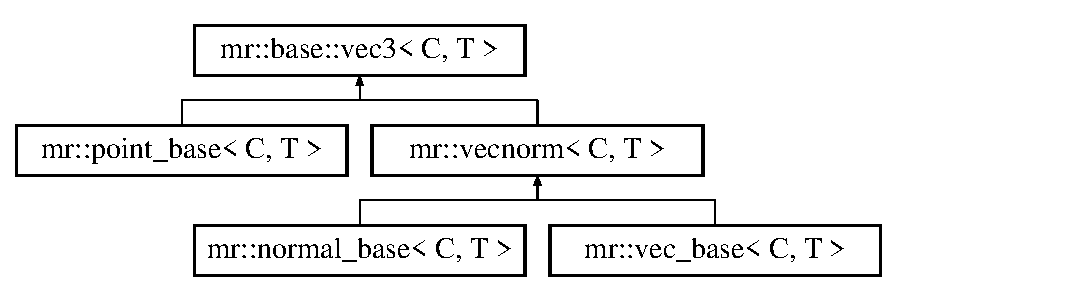
\includegraphics[height=3cm]{structmr_1_1base_1_1vec3}
\end{center}
\end{figure}
\subsection*{Public Types}
\begin{CompactItemize}
\item 
typedef {\bf vec3}$<$ C, T $>$ {\bf self}
\end{CompactItemize}
\subsection*{Public Member Functions}
\begin{CompactItemize}
\item 
const T {\bf Evaluate} (const unsigned short i) const 
\item 
{\bf operator mi\-Color} ()
\begin{CompactList}\small\item\em Conversion to mi\-Color. \item\end{CompactList}\item 
{\bf operator color} ()
\begin{CompactList}\small\item\em Conversion to color. \item\end{CompactList}\item 
{\bf vec3} ()
\begin{CompactList}\small\item\em Constructor that initializes x,y,z to 0. \item\end{CompactList}\item 
{\bf vec3} (const T xx, const T yy, const T zz)
\begin{CompactList}\small\item\em Constructor to initialize from three values. \item\end{CompactList}\item 
const bool {\bf is\-Equivalent} (const C \&b, const T tolerance=mi\-SCALAR\_\-EPSILON) const 
\item 
const {\bf self} \& {\bf mix} (const C \&b, const mi\-Scalar p)
\end{CompactItemize}
\begin{Indent}{\bf Accessors}\par
\begin{CompactItemize}
\item 
T \& {\bf operator[$\,$]} (const unsigned short i)
\begin{CompactList}\small\item\em Allow access to each element of vector for assignment. \item\end{CompactList}\item 
const T {\bf operator[$\,$]} (const unsigned short i) const 
\begin{CompactList}\small\item\em Allow access to each element of vector for reading. \item\end{CompactList}\item 
void {\bf set} (const unsigned short i, const T t)
\begin{CompactList}\small\item\em Allow assignment to an element of a vector. \item\end{CompactList}\item 
void {\bf set} (const T xx, const T yy, const T zz)
\begin{CompactList}\small\item\em Allow assignment to elements of a vector. \item\end{CompactList}\item 
T {\bf get} (const unsigned short i) const 
\begin{CompactList}\small\item\em Allow access to an element of vector for reading. \item\end{CompactList}\end{CompactItemize}
\end{Indent}
\begin{Indent}{\bf Assignment}\par
\begin{CompactItemize}
\item 
template$<$class X, class Y, class Oper$>$ const {\bf self} \& {\bf operator=} (const {\bf base::exp}$<$ X, Y, Oper $>$ \&e)
\begin{CompactList}\small\item\em Handle assignment when we deal with a chained operation. \item\end{CompactList}\item 
const {\bf self} \& {\bf operator=} (const {\bf self} \&b)
\begin{CompactList}\small\item\em Assignment of similar object. \item\end{CompactList}\item 
const {\bf self} \& {\bf operator=} (const C \&b)
\begin{CompactList}\small\item\em Assignemnt of base class object. \item\end{CompactList}\item 
const {\bf self} \& {\bf operator=} (const T b)
\begin{CompactList}\small\item\em Assignment of base type. \item\end{CompactList}\end{CompactItemize}
\end{Indent}
\begin{Indent}{\bf Equality}\par
\begin{CompactItemize}
\item 
template$<$class X, class Y, class Oper$>$ const bool {\bf operator==} (const {\bf base::exp}$<$ X, Y, Oper $>$ \&x) const 
\item 
const bool {\bf operator==} (const {\bf self} \&b) const 
\item 
const bool {\bf operator==} (const mi\-Vector \&b) const 
\item 
const bool {\bf operator==} (const T b) const 
\end{CompactItemize}
\end{Indent}
\begin{Indent}{\bf Inequality}\par
\begin{CompactItemize}
\item 
template$<$class X, class Y, class Oper$>$ const bool {\bf operator!=} (const {\bf base::exp}$<$ X, Y, Oper $>$ \&b) const 
\item 
const bool {\bf operator!=} (const {\bf self} \&b) const 
\item 
const bool {\bf operator!=} (const mi\-Vector \&b) const 
\item 
const bool {\bf operator!=} (const T b) const 
\end{CompactItemize}
\end{Indent}
\begin{Indent}{\bf REFERENCE OPERATORS (MODIFY IN PLACE)}\par
\begin{CompactItemize}
\item 
template$<$class X, class Y, class Oper$>$ const {\bf self} \& {\bf operator+=} (const {\bf base::exp}$<$ X, Y, Oper $>$ \&b)
\item 
const {\bf self} \& {\bf operator+=} (const T b)
\item 
const {\bf self} \& {\bf operator+=} (const C \&b)
\item 
template$<$class X, class Y, class Oper$>$ const {\bf self} \& {\bf operator-=} (const {\bf base::exp}$<$ X, Y, Oper $>$ \&b)
\item 
const {\bf self} \& {\bf operator-=} (const T b)
\item 
const {\bf self} \& {\bf operator-=} (const C \&b)
\item 
template$<$class X, class Y, class Oper$>$ const {\bf self} \& {\bf operator $\ast$=} (const {\bf base::exp}$<$ X, Y, Oper $>$ \&b)
\item 
const {\bf self} \& {\bf operator $\ast$=} (const T b)
\item 
const {\bf self} \& {\bf operator $\ast$=} (const C \&b)
\item 
template$<$class X, class Y, class Oper$>$ const {\bf self} \& {\bf operator/=} (const {\bf base::exp}$<$ X, Y, Oper $>$ \&b)
\item 
const {\bf self} \& {\bf operator/=} (const T b)
\item 
const {\bf self} \& {\bf operator/=} (const C \&b)
\end{CompactItemize}
\end{Indent}
\begin{Indent}{\bf Per channel comparisons}\par
\begin{CompactItemize}
\item 
{\bf self} {\bf less\-Than} (const C \&b)
\item 
{\bf self} {\bf less\-Than\-Equal} (const C \&b)
\item 
{\bf self} {\bf greater\-Than} (const C \&b)
\item 
{\bf self} {\bf greater\-Than\-Equal} (const C \&b)
\item 
const bool {\bf any} ()
\end{CompactItemize}
\end{Indent}
\begin{Indent}{\bf SWIZZLE OPERATORS}\par
\begin{CompactItemize}
\item 
const {\bf self} \& {\bf xyz} (const C \&t)
\item 
const {\bf self} \& {\bf xyz} (const {\bf self} \&t)
\item 
const {\bf self} \& {\bf xyz} () const 
\item 
const {\bf self} \& {\bf xyz} ()
\item 
{\bf self} {\bf xxx} () const 
\item 
{\bf self} {\bf yyy} () const 
\item 
{\bf self} {\bf zzz} () const 
\item 
{\bf self} {\bf zxy} () const 
\item 
{\bf self} {\bf yzx} () const 
\item 
{\bf self} {\bf zyx} () const 
\item 
{\bf self} {\bf yxz} () const 
\item 
{\bf self} {\bf yxx} () const 
\item 
{\bf self} {\bf zxx} () const 
\item 
{\bf self} {\bf xyx} () const 
\item 
{\bf self} {\bf xzx} () const 
\item 
{\bf self} {\bf xxy} () const 
\item 
{\bf self} {\bf xxz} () const 
\item 
{\bf self} {\bf xyy} () const 
\item 
{\bf self} {\bf zyy} () const 
\item 
{\bf self} {\bf yxy} () const 
\item 
{\bf self} {\bf yzy} () const 
\item 
{\bf self} {\bf yyx} () const 
\item 
{\bf self} {\bf yyz} () const 
\item 
{\bf self} {\bf yzz} () const 
\item 
{\bf self} {\bf xzz} () const 
\item 
{\bf self} {\bf zyz} () const 
\item 
{\bf self} {\bf zxz} () const 
\item 
{\bf self} {\bf zzy} () const 
\item 
{\bf self} {\bf zzx} () const 
\end{CompactItemize}
\end{Indent}
\subsubsection*{template$<$class C, class T$>$ struct mr::base::vec3$<$ C, T $>$}



\subsection{Member Typedef Documentation}
\index{mr::base::vec3@{mr::base::vec3}!self@{self}}
\index{self@{self}!mr::base::vec3@{mr::base::vec3}}
\subsubsection{\setlength{\rightskip}{0pt plus 5cm}template$<$class C, class T$>$ typedef {\bf vec3}$<$ C, T $>$ {\bf mr::base::vec3}$<$ C, T $>$::{\bf self}}\label{structmr_1_1base_1_1vec3_w0}




Reimplemented in {\bf mr::vecnorm$<$ C, T $>$} {\rm (p.\,\pageref{structmr_1_1vecnorm_w0})}, {\bf mr::vec\_\-base$<$ C, T $>$} {\rm (p.\,\pageref{structmr_1_1vec__base_w0})}, {\bf mr::normal\_\-base$<$ C, T $>$} {\rm (p.\,\pageref{structmr_1_1normal__base_w0})}, and {\bf mr::point\_\-base$<$ C, T $>$} {\rm (p.\,\pageref{structmr_1_1point__base_w0})}.

\subsection{Constructor \& Destructor Documentation}
\index{mr::base::vec3@{mr::base::vec3}!vec3@{vec3}}
\index{vec3@{vec3}!mr::base::vec3@{mr::base::vec3}}
\subsubsection{\setlength{\rightskip}{0pt plus 5cm}template$<$class C, class T$>$ {\bf mr::base::vec3}$<$ C, T $>$::{\bf vec3} ()\hspace{0.3cm}{\tt  [inline]}}\label{structmr_1_1base_1_1vec3_a3}


Constructor that initializes x,y,z to 0. 

\index{mr::base::vec3@{mr::base::vec3}!vec3@{vec3}}
\index{vec3@{vec3}!mr::base::vec3@{mr::base::vec3}}
\subsubsection{\setlength{\rightskip}{0pt plus 5cm}template$<$class C, class T$>$ {\bf mr::base::vec3}$<$ C, T $>$::{\bf vec3} (const T {\em xx}, const T {\em yy}, const T {\em zz})\hspace{0.3cm}{\tt  [inline]}}\label{structmr_1_1base_1_1vec3_a4}


Constructor to initialize from three values. 



\subsection{Member Function Documentation}
\index{mr::base::vec3@{mr::base::vec3}!any@{any}}
\index{any@{any}!mr::base::vec3@{mr::base::vec3}}
\subsubsection{\setlength{\rightskip}{0pt plus 5cm}template$<$class C, class T$>$ const bool {\bf mr::base::vec3}$<$ C, T $>$::any ()\hspace{0.3cm}{\tt  [inline]}}\label{structmr_1_1base_1_1vec3_z42_4}


\index{mr::base::vec3@{mr::base::vec3}!Evaluate@{Evaluate}}
\index{Evaluate@{Evaluate}!mr::base::vec3@{mr::base::vec3}}
\subsubsection{\setlength{\rightskip}{0pt plus 5cm}template$<$class C, class T$>$ const T {\bf mr::base::vec3}$<$ C, T $>$::Evaluate (const unsigned short {\em i}) const\hspace{0.3cm}{\tt  [inline]}}\label{structmr_1_1base_1_1vec3_a0}


\index{mr::base::vec3@{mr::base::vec3}!get@{get}}
\index{get@{get}!mr::base::vec3@{mr::base::vec3}}
\subsubsection{\setlength{\rightskip}{0pt plus 5cm}template$<$class C, class T$>$ T {\bf mr::base::vec3}$<$ C, T $>$::get (const unsigned short {\em i}) const\hspace{0.3cm}{\tt  [inline]}}\label{structmr_1_1base_1_1vec3_z35_4}


Allow access to an element of vector for reading. 

\index{mr::base::vec3@{mr::base::vec3}!greaterThan@{greaterThan}}
\index{greaterThan@{greaterThan}!mr::base::vec3@{mr::base::vec3}}
\subsubsection{\setlength{\rightskip}{0pt plus 5cm}template$<$class C, class T$>$ {\bf self} {\bf mr::base::vec3}$<$ C, T $>$::greater\-Than (const C \& {\em b})\hspace{0.3cm}{\tt  [inline]}}\label{structmr_1_1base_1_1vec3_z42_2}


\index{mr::base::vec3@{mr::base::vec3}!greaterThanEqual@{greaterThanEqual}}
\index{greaterThanEqual@{greaterThanEqual}!mr::base::vec3@{mr::base::vec3}}
\subsubsection{\setlength{\rightskip}{0pt plus 5cm}template$<$class C, class T$>$ {\bf self} {\bf mr::base::vec3}$<$ C, T $>$::greater\-Than\-Equal (const C \& {\em b})\hspace{0.3cm}{\tt  [inline]}}\label{structmr_1_1base_1_1vec3_z42_3}


\index{mr::base::vec3@{mr::base::vec3}!isEquivalent@{isEquivalent}}
\index{isEquivalent@{isEquivalent}!mr::base::vec3@{mr::base::vec3}}
\subsubsection{\setlength{\rightskip}{0pt plus 5cm}template$<$class C, class T$>$ const bool {\bf mr::base::vec3}$<$ C, T $>$::is\-Equivalent (const C \& {\em b}, const T {\em tolerance} = mi\-SCALAR\_\-EPSILON) const\hspace{0.3cm}{\tt  [inline]}}\label{structmr_1_1base_1_1vec3_a5}


\index{mr::base::vec3@{mr::base::vec3}!lessThan@{lessThan}}
\index{lessThan@{lessThan}!mr::base::vec3@{mr::base::vec3}}
\subsubsection{\setlength{\rightskip}{0pt plus 5cm}template$<$class C, class T$>$ {\bf self} {\bf mr::base::vec3}$<$ C, T $>$::less\-Than (const C \& {\em b})\hspace{0.3cm}{\tt  [inline]}}\label{structmr_1_1base_1_1vec3_z42_0}


\index{mr::base::vec3@{mr::base::vec3}!lessThanEqual@{lessThanEqual}}
\index{lessThanEqual@{lessThanEqual}!mr::base::vec3@{mr::base::vec3}}
\subsubsection{\setlength{\rightskip}{0pt plus 5cm}template$<$class C, class T$>$ {\bf self} {\bf mr::base::vec3}$<$ C, T $>$::less\-Than\-Equal (const C \& {\em b})\hspace{0.3cm}{\tt  [inline]}}\label{structmr_1_1base_1_1vec3_z42_1}


\index{mr::base::vec3@{mr::base::vec3}!mix@{mix}}
\index{mix@{mix}!mr::base::vec3@{mr::base::vec3}}
\subsubsection{\setlength{\rightskip}{0pt plus 5cm}template$<$class C, class T$>$ const {\bf self}\& {\bf mr::base::vec3}$<$ C, T $>$::mix (const C \& {\em b}, const mi\-Scalar {\em p})\hspace{0.3cm}{\tt  [inline]}}\label{structmr_1_1base_1_1vec3_a6}


\index{mr::base::vec3@{mr::base::vec3}!operator *=@{operator $\ast$=}}
\index{operator *=@{operator $\ast$=}!mr::base::vec3@{mr::base::vec3}}
\subsubsection{\setlength{\rightskip}{0pt plus 5cm}template$<$class C, class T$>$ const {\bf self}\& {\bf mr::base::vec3}$<$ C, T $>$::operator $\ast$= (const C \& {\em b})\hspace{0.3cm}{\tt  [inline]}}\label{structmr_1_1base_1_1vec3_z40_8}




Reimplemented in {\bf mr::vec\_\-base$<$ C, T $>$} {\rm (p.\,\pageref{structmr_1_1vec__base_z64_1})}, {\bf mr::normal\_\-base$<$ C, T $>$} {\rm (p.\,\pageref{structmr_1_1normal__base_z71_1})}, and {\bf mr::point\_\-base$<$ C, T $>$} {\rm (p.\,\pageref{structmr_1_1point__base_z78_1})}.\index{mr::base::vec3@{mr::base::vec3}!operator *=@{operator $\ast$=}}
\index{operator *=@{operator $\ast$=}!mr::base::vec3@{mr::base::vec3}}
\subsubsection{\setlength{\rightskip}{0pt plus 5cm}template$<$class C, class T$>$ const {\bf self}\& {\bf mr::base::vec3}$<$ C, T $>$::operator $\ast$= (const T {\em b})\hspace{0.3cm}{\tt  [inline]}}\label{structmr_1_1base_1_1vec3_z40_7}




Reimplemented in {\bf mr::vec\_\-base$<$ C, T $>$} {\rm (p.\,\pageref{structmr_1_1vec__base_z64_0})}, {\bf mr::normal\_\-base$<$ C, T $>$} {\rm (p.\,\pageref{structmr_1_1normal__base_z71_0})}, and {\bf mr::point\_\-base$<$ C, T $>$} {\rm (p.\,\pageref{structmr_1_1point__base_z78_0})}.\index{mr::base::vec3@{mr::base::vec3}!operator *=@{operator $\ast$=}}
\index{operator *=@{operator $\ast$=}!mr::base::vec3@{mr::base::vec3}}
\subsubsection{\setlength{\rightskip}{0pt plus 5cm}template$<$class C, class T$>$ template$<$class X, class Y, class Oper$>$ const {\bf self}\& {\bf mr::base::vec3}$<$ C, T $>$::operator $\ast$= (const {\bf base::exp}$<$ X, Y, Oper $>$ \& {\em b})\hspace{0.3cm}{\tt  [inline]}}\label{structmr_1_1base_1_1vec3_z40_6}


\index{mr::base::vec3@{mr::base::vec3}!operator color@{operator color}}
\index{operator color@{operator color}!mr::base::vec3@{mr::base::vec3}}
\subsubsection{\setlength{\rightskip}{0pt plus 5cm}template$<$class C, class T$>$ {\bf mr::base::vec3}$<$ C, T $>$::operator {\bf color} ()\hspace{0.3cm}{\tt  [inline]}}\label{structmr_1_1base_1_1vec3_a2}


Conversion to color. 

\index{mr::base::vec3@{mr::base::vec3}!operator miColor@{operator miColor}}
\index{operator miColor@{operator miColor}!mr::base::vec3@{mr::base::vec3}}
\subsubsection{\setlength{\rightskip}{0pt plus 5cm}template$<$class C, class T$>$ {\bf mr::base::vec3}$<$ C, T $>$::operator mi\-Color ()\hspace{0.3cm}{\tt  [inline]}}\label{structmr_1_1base_1_1vec3_a1}


Conversion to mi\-Color. 

\index{mr::base::vec3@{mr::base::vec3}!operator"!=@{operator"!=}}
\index{operator"!=@{operator"!=}!mr::base::vec3@{mr::base::vec3}}
\subsubsection{\setlength{\rightskip}{0pt plus 5cm}template$<$class C, class T$>$ const bool {\bf mr::base::vec3}$<$ C, T $>$::operator!= (const T {\em b}) const\hspace{0.3cm}{\tt  [inline]}}\label{structmr_1_1base_1_1vec3_z38_3}


\index{mr::base::vec3@{mr::base::vec3}!operator"!=@{operator"!=}}
\index{operator"!=@{operator"!=}!mr::base::vec3@{mr::base::vec3}}
\subsubsection{\setlength{\rightskip}{0pt plus 5cm}template$<$class C, class T$>$ const bool {\bf mr::base::vec3}$<$ C, T $>$::operator!= (const mi\-Vector \& {\em b}) const\hspace{0.3cm}{\tt  [inline]}}\label{structmr_1_1base_1_1vec3_z38_2}


\index{mr::base::vec3@{mr::base::vec3}!operator"!=@{operator"!=}}
\index{operator"!=@{operator"!=}!mr::base::vec3@{mr::base::vec3}}
\subsubsection{\setlength{\rightskip}{0pt plus 5cm}template$<$class C, class T$>$ const bool {\bf mr::base::vec3}$<$ C, T $>$::operator!= (const {\bf self} \& {\em b}) const\hspace{0.3cm}{\tt  [inline]}}\label{structmr_1_1base_1_1vec3_z38_1}


\index{mr::base::vec3@{mr::base::vec3}!operator"!=@{operator"!=}}
\index{operator"!=@{operator"!=}!mr::base::vec3@{mr::base::vec3}}
\subsubsection{\setlength{\rightskip}{0pt plus 5cm}template$<$class C, class T$>$ template$<$class X, class Y, class Oper$>$ const bool {\bf mr::base::vec3}$<$ C, T $>$::operator!= (const {\bf base::exp}$<$ X, Y, Oper $>$ \& {\em b}) const\hspace{0.3cm}{\tt  [inline]}}\label{structmr_1_1base_1_1vec3_z38_0}


\index{mr::base::vec3@{mr::base::vec3}!operator+=@{operator+=}}
\index{operator+=@{operator+=}!mr::base::vec3@{mr::base::vec3}}
\subsubsection{\setlength{\rightskip}{0pt plus 5cm}template$<$class C, class T$>$ const {\bf self}\& {\bf mr::base::vec3}$<$ C, T $>$::operator+= (const C \& {\em b})\hspace{0.3cm}{\tt  [inline]}}\label{structmr_1_1base_1_1vec3_z40_2}


\index{mr::base::vec3@{mr::base::vec3}!operator+=@{operator+=}}
\index{operator+=@{operator+=}!mr::base::vec3@{mr::base::vec3}}
\subsubsection{\setlength{\rightskip}{0pt plus 5cm}template$<$class C, class T$>$ const {\bf self}\& {\bf mr::base::vec3}$<$ C, T $>$::operator+= (const T {\em b})\hspace{0.3cm}{\tt  [inline]}}\label{structmr_1_1base_1_1vec3_z40_1}


\index{mr::base::vec3@{mr::base::vec3}!operator+=@{operator+=}}
\index{operator+=@{operator+=}!mr::base::vec3@{mr::base::vec3}}
\subsubsection{\setlength{\rightskip}{0pt plus 5cm}template$<$class C, class T$>$ template$<$class X, class Y, class Oper$>$ const {\bf self}\& {\bf mr::base::vec3}$<$ C, T $>$::operator+= (const {\bf base::exp}$<$ X, Y, Oper $>$ \& {\em b})\hspace{0.3cm}{\tt  [inline]}}\label{structmr_1_1base_1_1vec3_z40_0}


\index{mr::base::vec3@{mr::base::vec3}!operator-=@{operator-=}}
\index{operator-=@{operator-=}!mr::base::vec3@{mr::base::vec3}}
\subsubsection{\setlength{\rightskip}{0pt plus 5cm}template$<$class C, class T$>$ const {\bf self}\& {\bf mr::base::vec3}$<$ C, T $>$::operator-= (const C \& {\em b})\hspace{0.3cm}{\tt  [inline]}}\label{structmr_1_1base_1_1vec3_z40_5}


\index{mr::base::vec3@{mr::base::vec3}!operator-=@{operator-=}}
\index{operator-=@{operator-=}!mr::base::vec3@{mr::base::vec3}}
\subsubsection{\setlength{\rightskip}{0pt plus 5cm}template$<$class C, class T$>$ const {\bf self}\& {\bf mr::base::vec3}$<$ C, T $>$::operator-= (const T {\em b})\hspace{0.3cm}{\tt  [inline]}}\label{structmr_1_1base_1_1vec3_z40_4}


\index{mr::base::vec3@{mr::base::vec3}!operator-=@{operator-=}}
\index{operator-=@{operator-=}!mr::base::vec3@{mr::base::vec3}}
\subsubsection{\setlength{\rightskip}{0pt plus 5cm}template$<$class C, class T$>$ template$<$class X, class Y, class Oper$>$ const {\bf self}\& {\bf mr::base::vec3}$<$ C, T $>$::operator-= (const {\bf base::exp}$<$ X, Y, Oper $>$ \& {\em b})\hspace{0.3cm}{\tt  [inline]}}\label{structmr_1_1base_1_1vec3_z40_3}


\index{mr::base::vec3@{mr::base::vec3}!operator/=@{operator/=}}
\index{operator/=@{operator/=}!mr::base::vec3@{mr::base::vec3}}
\subsubsection{\setlength{\rightskip}{0pt plus 5cm}template$<$class C, class T$>$ const {\bf self}\& {\bf mr::base::vec3}$<$ C, T $>$::operator/= (const C \& {\em b})\hspace{0.3cm}{\tt  [inline]}}\label{structmr_1_1base_1_1vec3_z40_11}


\index{mr::base::vec3@{mr::base::vec3}!operator/=@{operator/=}}
\index{operator/=@{operator/=}!mr::base::vec3@{mr::base::vec3}}
\subsubsection{\setlength{\rightskip}{0pt plus 5cm}template$<$class C, class T$>$ const {\bf self}\& {\bf mr::base::vec3}$<$ C, T $>$::operator/= (const T {\em b})\hspace{0.3cm}{\tt  [inline]}}\label{structmr_1_1base_1_1vec3_z40_10}


\index{mr::base::vec3@{mr::base::vec3}!operator/=@{operator/=}}
\index{operator/=@{operator/=}!mr::base::vec3@{mr::base::vec3}}
\subsubsection{\setlength{\rightskip}{0pt plus 5cm}template$<$class C, class T$>$ template$<$class X, class Y, class Oper$>$ const {\bf self}\& {\bf mr::base::vec3}$<$ C, T $>$::operator/= (const {\bf base::exp}$<$ X, Y, Oper $>$ \& {\em b})\hspace{0.3cm}{\tt  [inline]}}\label{structmr_1_1base_1_1vec3_z40_9}


\index{mr::base::vec3@{mr::base::vec3}!operator=@{operator=}}
\index{operator=@{operator=}!mr::base::vec3@{mr::base::vec3}}
\subsubsection{\setlength{\rightskip}{0pt plus 5cm}template$<$class C, class T$>$ const {\bf self}\& {\bf mr::base::vec3}$<$ C, T $>$::operator= (const T {\em b})\hspace{0.3cm}{\tt  [inline]}}\label{structmr_1_1base_1_1vec3_z36_3}


Assignment of base type. 



Reimplemented in {\bf mr::vec\_\-base$<$ C, T $>$} {\rm (p.\,\pageref{structmr_1_1vec__base_z60_3})}, {\bf mr::normal\_\-base$<$ C, T $>$} {\rm (p.\,\pageref{structmr_1_1normal__base_z69_3})}, and {\bf mr::point\_\-base$<$ C, T $>$} {\rm (p.\,\pageref{structmr_1_1point__base_z77_3})}.\index{mr::base::vec3@{mr::base::vec3}!operator=@{operator=}}
\index{operator=@{operator=}!mr::base::vec3@{mr::base::vec3}}
\subsubsection{\setlength{\rightskip}{0pt plus 5cm}template$<$class C, class T$>$ const {\bf self}\& {\bf mr::base::vec3}$<$ C, T $>$::operator= (const C \& {\em b})\hspace{0.3cm}{\tt  [inline]}}\label{structmr_1_1base_1_1vec3_z36_2}


Assignemnt of base class object. 



Reimplemented in {\bf mr::vec\_\-base$<$ C, T $>$} {\rm (p.\,\pageref{structmr_1_1vec__base_z60_2})}, {\bf mr::normal\_\-base$<$ C, T $>$} {\rm (p.\,\pageref{structmr_1_1normal__base_z69_2})}, and {\bf mr::point\_\-base$<$ C, T $>$} {\rm (p.\,\pageref{structmr_1_1point__base_z77_2})}.\index{mr::base::vec3@{mr::base::vec3}!operator=@{operator=}}
\index{operator=@{operator=}!mr::base::vec3@{mr::base::vec3}}
\subsubsection{\setlength{\rightskip}{0pt plus 5cm}template$<$class C, class T$>$ const {\bf self}\& {\bf mr::base::vec3}$<$ C, T $>$::operator= (const {\bf self} \& {\em b})\hspace{0.3cm}{\tt  [inline]}}\label{structmr_1_1base_1_1vec3_z36_1}


Assignment of similar object. 



Reimplemented in {\bf mr::vec\_\-base$<$ C, T $>$} {\rm (p.\,\pageref{structmr_1_1vec__base_z60_1})}, {\bf mr::normal\_\-base$<$ C, T $>$} {\rm (p.\,\pageref{structmr_1_1normal__base_z69_1})}, and {\bf mr::point\_\-base$<$ C, T $>$} {\rm (p.\,\pageref{structmr_1_1point__base_z77_1})}.\index{mr::base::vec3@{mr::base::vec3}!operator=@{operator=}}
\index{operator=@{operator=}!mr::base::vec3@{mr::base::vec3}}
\subsubsection{\setlength{\rightskip}{0pt plus 5cm}template$<$class C, class T$>$ template$<$class X, class Y, class Oper$>$ const {\bf self}\& {\bf mr::base::vec3}$<$ C, T $>$::operator= (const {\bf base::exp}$<$ X, Y, Oper $>$ \& {\em e})\hspace{0.3cm}{\tt  [inline]}}\label{structmr_1_1base_1_1vec3_z36_0}


Handle assignment when we deal with a chained operation. 



Reimplemented in {\bf mr::vec\_\-base$<$ C, T $>$} {\rm (p.\,\pageref{structmr_1_1vec__base_z60_0})}, {\bf mr::normal\_\-base$<$ C, T $>$} {\rm (p.\,\pageref{structmr_1_1normal__base_z69_0})}, and {\bf mr::point\_\-base$<$ C, T $>$} {\rm (p.\,\pageref{structmr_1_1point__base_z77_0})}.\index{mr::base::vec3@{mr::base::vec3}!operator==@{operator==}}
\index{operator==@{operator==}!mr::base::vec3@{mr::base::vec3}}
\subsubsection{\setlength{\rightskip}{0pt plus 5cm}template$<$class C, class T$>$ const bool {\bf mr::base::vec3}$<$ C, T $>$::operator== (const T {\em b}) const\hspace{0.3cm}{\tt  [inline]}}\label{structmr_1_1base_1_1vec3_z37_3}


\index{mr::base::vec3@{mr::base::vec3}!operator==@{operator==}}
\index{operator==@{operator==}!mr::base::vec3@{mr::base::vec3}}
\subsubsection{\setlength{\rightskip}{0pt plus 5cm}template$<$class C, class T$>$ const bool {\bf mr::base::vec3}$<$ C, T $>$::operator== (const mi\-Vector \& {\em b}) const\hspace{0.3cm}{\tt  [inline]}}\label{structmr_1_1base_1_1vec3_z37_2}


\index{mr::base::vec3@{mr::base::vec3}!operator==@{operator==}}
\index{operator==@{operator==}!mr::base::vec3@{mr::base::vec3}}
\subsubsection{\setlength{\rightskip}{0pt plus 5cm}template$<$class C, class T$>$ const bool {\bf mr::base::vec3}$<$ C, T $>$::operator== (const {\bf self} \& {\em b}) const\hspace{0.3cm}{\tt  [inline]}}\label{structmr_1_1base_1_1vec3_z37_1}


\index{mr::base::vec3@{mr::base::vec3}!operator==@{operator==}}
\index{operator==@{operator==}!mr::base::vec3@{mr::base::vec3}}
\subsubsection{\setlength{\rightskip}{0pt plus 5cm}template$<$class C, class T$>$ template$<$class X, class Y, class Oper$>$ const bool {\bf mr::base::vec3}$<$ C, T $>$::operator== (const {\bf base::exp}$<$ X, Y, Oper $>$ \& {\em x}) const\hspace{0.3cm}{\tt  [inline]}}\label{structmr_1_1base_1_1vec3_z37_0}


\index{mr::base::vec3@{mr::base::vec3}!operator[]@{operator[]}}
\index{operator[]@{operator[]}!mr::base::vec3@{mr::base::vec3}}
\subsubsection{\setlength{\rightskip}{0pt plus 5cm}template$<$class C, class T$>$ const T {\bf mr::base::vec3}$<$ C, T $>$::operator[$\,$] (const unsigned short {\em i}) const\hspace{0.3cm}{\tt  [inline]}}\label{structmr_1_1base_1_1vec3_z35_1}


Allow access to each element of vector for reading. 

\index{mr::base::vec3@{mr::base::vec3}!operator[]@{operator[]}}
\index{operator[]@{operator[]}!mr::base::vec3@{mr::base::vec3}}
\subsubsection{\setlength{\rightskip}{0pt plus 5cm}template$<$class C, class T$>$ T\& {\bf mr::base::vec3}$<$ C, T $>$::operator[$\,$] (const unsigned short {\em i})\hspace{0.3cm}{\tt  [inline]}}\label{structmr_1_1base_1_1vec3_z35_0}


Allow access to each element of vector for assignment. 

\index{mr::base::vec3@{mr::base::vec3}!set@{set}}
\index{set@{set}!mr::base::vec3@{mr::base::vec3}}
\subsubsection{\setlength{\rightskip}{0pt plus 5cm}template$<$class C, class T$>$ void {\bf mr::base::vec3}$<$ C, T $>$::set (const T {\em xx}, const T {\em yy}, const T {\em zz})\hspace{0.3cm}{\tt  [inline]}}\label{structmr_1_1base_1_1vec3_z35_3}


Allow assignment to elements of a vector. 

\index{mr::base::vec3@{mr::base::vec3}!set@{set}}
\index{set@{set}!mr::base::vec3@{mr::base::vec3}}
\subsubsection{\setlength{\rightskip}{0pt plus 5cm}template$<$class C, class T$>$ void {\bf mr::base::vec3}$<$ C, T $>$::set (const unsigned short {\em i}, const T {\em t})\hspace{0.3cm}{\tt  [inline]}}\label{structmr_1_1base_1_1vec3_z35_2}


Allow assignment to an element of a vector. 

\index{mr::base::vec3@{mr::base::vec3}!xxx@{xxx}}
\index{xxx@{xxx}!mr::base::vec3@{mr::base::vec3}}
\subsubsection{\setlength{\rightskip}{0pt plus 5cm}template$<$class C, class T$>$ {\bf self} {\bf mr::base::vec3}$<$ C, T $>$::xxx () const\hspace{0.3cm}{\tt  [inline]}}\label{structmr_1_1base_1_1vec3_z44_4}


\index{mr::base::vec3@{mr::base::vec3}!xxy@{xxy}}
\index{xxy@{xxy}!mr::base::vec3@{mr::base::vec3}}
\subsubsection{\setlength{\rightskip}{0pt plus 5cm}template$<$class C, class T$>$ {\bf self} {\bf mr::base::vec3}$<$ C, T $>$::xxy () const\hspace{0.3cm}{\tt  [inline]}}\label{structmr_1_1base_1_1vec3_z44_15}


\index{mr::base::vec3@{mr::base::vec3}!xxz@{xxz}}
\index{xxz@{xxz}!mr::base::vec3@{mr::base::vec3}}
\subsubsection{\setlength{\rightskip}{0pt plus 5cm}template$<$class C, class T$>$ {\bf self} {\bf mr::base::vec3}$<$ C, T $>$::xxz () const\hspace{0.3cm}{\tt  [inline]}}\label{structmr_1_1base_1_1vec3_z44_16}


\index{mr::base::vec3@{mr::base::vec3}!xyx@{xyx}}
\index{xyx@{xyx}!mr::base::vec3@{mr::base::vec3}}
\subsubsection{\setlength{\rightskip}{0pt plus 5cm}template$<$class C, class T$>$ {\bf self} {\bf mr::base::vec3}$<$ C, T $>$::xyx () const\hspace{0.3cm}{\tt  [inline]}}\label{structmr_1_1base_1_1vec3_z44_13}


\index{mr::base::vec3@{mr::base::vec3}!xyy@{xyy}}
\index{xyy@{xyy}!mr::base::vec3@{mr::base::vec3}}
\subsubsection{\setlength{\rightskip}{0pt plus 5cm}template$<$class C, class T$>$ {\bf self} {\bf mr::base::vec3}$<$ C, T $>$::xyy () const\hspace{0.3cm}{\tt  [inline]}}\label{structmr_1_1base_1_1vec3_z44_17}


\index{mr::base::vec3@{mr::base::vec3}!xyz@{xyz}}
\index{xyz@{xyz}!mr::base::vec3@{mr::base::vec3}}
\subsubsection{\setlength{\rightskip}{0pt plus 5cm}template$<$class C, class T$>$ const {\bf self}\& {\bf mr::base::vec3}$<$ C, T $>$::xyz ()\hspace{0.3cm}{\tt  [inline]}}\label{structmr_1_1base_1_1vec3_z44_3}


\index{mr::base::vec3@{mr::base::vec3}!xyz@{xyz}}
\index{xyz@{xyz}!mr::base::vec3@{mr::base::vec3}}
\subsubsection{\setlength{\rightskip}{0pt plus 5cm}template$<$class C, class T$>$ const {\bf self}\& {\bf mr::base::vec3}$<$ C, T $>$::xyz () const\hspace{0.3cm}{\tt  [inline]}}\label{structmr_1_1base_1_1vec3_z44_2}


\index{mr::base::vec3@{mr::base::vec3}!xyz@{xyz}}
\index{xyz@{xyz}!mr::base::vec3@{mr::base::vec3}}
\subsubsection{\setlength{\rightskip}{0pt plus 5cm}template$<$class C, class T$>$ const {\bf self}\& {\bf mr::base::vec3}$<$ C, T $>$::xyz (const {\bf self} \& {\em t})\hspace{0.3cm}{\tt  [inline]}}\label{structmr_1_1base_1_1vec3_z44_1}


\index{mr::base::vec3@{mr::base::vec3}!xyz@{xyz}}
\index{xyz@{xyz}!mr::base::vec3@{mr::base::vec3}}
\subsubsection{\setlength{\rightskip}{0pt plus 5cm}template$<$class C, class T$>$ const {\bf self}\& {\bf mr::base::vec3}$<$ C, T $>$::xyz (const C \& {\em t})\hspace{0.3cm}{\tt  [inline]}}\label{structmr_1_1base_1_1vec3_z44_0}


\index{mr::base::vec3@{mr::base::vec3}!xzx@{xzx}}
\index{xzx@{xzx}!mr::base::vec3@{mr::base::vec3}}
\subsubsection{\setlength{\rightskip}{0pt plus 5cm}template$<$class C, class T$>$ {\bf self} {\bf mr::base::vec3}$<$ C, T $>$::xzx () const\hspace{0.3cm}{\tt  [inline]}}\label{structmr_1_1base_1_1vec3_z44_14}


\index{mr::base::vec3@{mr::base::vec3}!xzz@{xzz}}
\index{xzz@{xzz}!mr::base::vec3@{mr::base::vec3}}
\subsubsection{\setlength{\rightskip}{0pt plus 5cm}template$<$class C, class T$>$ {\bf self} {\bf mr::base::vec3}$<$ C, T $>$::xzz () const\hspace{0.3cm}{\tt  [inline]}}\label{structmr_1_1base_1_1vec3_z44_24}


\index{mr::base::vec3@{mr::base::vec3}!yxx@{yxx}}
\index{yxx@{yxx}!mr::base::vec3@{mr::base::vec3}}
\subsubsection{\setlength{\rightskip}{0pt plus 5cm}template$<$class C, class T$>$ {\bf self} {\bf mr::base::vec3}$<$ C, T $>$::yxx () const\hspace{0.3cm}{\tt  [inline]}}\label{structmr_1_1base_1_1vec3_z44_11}


\index{mr::base::vec3@{mr::base::vec3}!yxy@{yxy}}
\index{yxy@{yxy}!mr::base::vec3@{mr::base::vec3}}
\subsubsection{\setlength{\rightskip}{0pt plus 5cm}template$<$class C, class T$>$ {\bf self} {\bf mr::base::vec3}$<$ C, T $>$::yxy () const\hspace{0.3cm}{\tt  [inline]}}\label{structmr_1_1base_1_1vec3_z44_19}


\index{mr::base::vec3@{mr::base::vec3}!yxz@{yxz}}
\index{yxz@{yxz}!mr::base::vec3@{mr::base::vec3}}
\subsubsection{\setlength{\rightskip}{0pt plus 5cm}template$<$class C, class T$>$ {\bf self} {\bf mr::base::vec3}$<$ C, T $>$::yxz () const\hspace{0.3cm}{\tt  [inline]}}\label{structmr_1_1base_1_1vec3_z44_10}


\index{mr::base::vec3@{mr::base::vec3}!yyx@{yyx}}
\index{yyx@{yyx}!mr::base::vec3@{mr::base::vec3}}
\subsubsection{\setlength{\rightskip}{0pt plus 5cm}template$<$class C, class T$>$ {\bf self} {\bf mr::base::vec3}$<$ C, T $>$::yyx () const\hspace{0.3cm}{\tt  [inline]}}\label{structmr_1_1base_1_1vec3_z44_21}


\index{mr::base::vec3@{mr::base::vec3}!yyy@{yyy}}
\index{yyy@{yyy}!mr::base::vec3@{mr::base::vec3}}
\subsubsection{\setlength{\rightskip}{0pt plus 5cm}template$<$class C, class T$>$ {\bf self} {\bf mr::base::vec3}$<$ C, T $>$::yyy () const\hspace{0.3cm}{\tt  [inline]}}\label{structmr_1_1base_1_1vec3_z44_5}


\index{mr::base::vec3@{mr::base::vec3}!yyz@{yyz}}
\index{yyz@{yyz}!mr::base::vec3@{mr::base::vec3}}
\subsubsection{\setlength{\rightskip}{0pt plus 5cm}template$<$class C, class T$>$ {\bf self} {\bf mr::base::vec3}$<$ C, T $>$::yyz () const\hspace{0.3cm}{\tt  [inline]}}\label{structmr_1_1base_1_1vec3_z44_22}


\index{mr::base::vec3@{mr::base::vec3}!yzx@{yzx}}
\index{yzx@{yzx}!mr::base::vec3@{mr::base::vec3}}
\subsubsection{\setlength{\rightskip}{0pt plus 5cm}template$<$class C, class T$>$ {\bf self} {\bf mr::base::vec3}$<$ C, T $>$::yzx () const\hspace{0.3cm}{\tt  [inline]}}\label{structmr_1_1base_1_1vec3_z44_8}


\index{mr::base::vec3@{mr::base::vec3}!yzy@{yzy}}
\index{yzy@{yzy}!mr::base::vec3@{mr::base::vec3}}
\subsubsection{\setlength{\rightskip}{0pt plus 5cm}template$<$class C, class T$>$ {\bf self} {\bf mr::base::vec3}$<$ C, T $>$::yzy () const\hspace{0.3cm}{\tt  [inline]}}\label{structmr_1_1base_1_1vec3_z44_20}


\index{mr::base::vec3@{mr::base::vec3}!yzz@{yzz}}
\index{yzz@{yzz}!mr::base::vec3@{mr::base::vec3}}
\subsubsection{\setlength{\rightskip}{0pt plus 5cm}template$<$class C, class T$>$ {\bf self} {\bf mr::base::vec3}$<$ C, T $>$::yzz () const\hspace{0.3cm}{\tt  [inline]}}\label{structmr_1_1base_1_1vec3_z44_23}


\index{mr::base::vec3@{mr::base::vec3}!zxx@{zxx}}
\index{zxx@{zxx}!mr::base::vec3@{mr::base::vec3}}
\subsubsection{\setlength{\rightskip}{0pt plus 5cm}template$<$class C, class T$>$ {\bf self} {\bf mr::base::vec3}$<$ C, T $>$::zxx () const\hspace{0.3cm}{\tt  [inline]}}\label{structmr_1_1base_1_1vec3_z44_12}


\index{mr::base::vec3@{mr::base::vec3}!zxy@{zxy}}
\index{zxy@{zxy}!mr::base::vec3@{mr::base::vec3}}
\subsubsection{\setlength{\rightskip}{0pt plus 5cm}template$<$class C, class T$>$ {\bf self} {\bf mr::base::vec3}$<$ C, T $>$::zxy () const\hspace{0.3cm}{\tt  [inline]}}\label{structmr_1_1base_1_1vec3_z44_7}


\index{mr::base::vec3@{mr::base::vec3}!zxz@{zxz}}
\index{zxz@{zxz}!mr::base::vec3@{mr::base::vec3}}
\subsubsection{\setlength{\rightskip}{0pt plus 5cm}template$<$class C, class T$>$ {\bf self} {\bf mr::base::vec3}$<$ C, T $>$::zxz () const\hspace{0.3cm}{\tt  [inline]}}\label{structmr_1_1base_1_1vec3_z44_26}


\index{mr::base::vec3@{mr::base::vec3}!zyx@{zyx}}
\index{zyx@{zyx}!mr::base::vec3@{mr::base::vec3}}
\subsubsection{\setlength{\rightskip}{0pt plus 5cm}template$<$class C, class T$>$ {\bf self} {\bf mr::base::vec3}$<$ C, T $>$::zyx () const\hspace{0.3cm}{\tt  [inline]}}\label{structmr_1_1base_1_1vec3_z44_9}


\index{mr::base::vec3@{mr::base::vec3}!zyy@{zyy}}
\index{zyy@{zyy}!mr::base::vec3@{mr::base::vec3}}
\subsubsection{\setlength{\rightskip}{0pt plus 5cm}template$<$class C, class T$>$ {\bf self} {\bf mr::base::vec3}$<$ C, T $>$::zyy () const\hspace{0.3cm}{\tt  [inline]}}\label{structmr_1_1base_1_1vec3_z44_18}


\index{mr::base::vec3@{mr::base::vec3}!zyz@{zyz}}
\index{zyz@{zyz}!mr::base::vec3@{mr::base::vec3}}
\subsubsection{\setlength{\rightskip}{0pt plus 5cm}template$<$class C, class T$>$ {\bf self} {\bf mr::base::vec3}$<$ C, T $>$::zyz () const\hspace{0.3cm}{\tt  [inline]}}\label{structmr_1_1base_1_1vec3_z44_25}


\index{mr::base::vec3@{mr::base::vec3}!zzx@{zzx}}
\index{zzx@{zzx}!mr::base::vec3@{mr::base::vec3}}
\subsubsection{\setlength{\rightskip}{0pt plus 5cm}template$<$class C, class T$>$ {\bf self} {\bf mr::base::vec3}$<$ C, T $>$::zzx () const\hspace{0.3cm}{\tt  [inline]}}\label{structmr_1_1base_1_1vec3_z44_28}


\index{mr::base::vec3@{mr::base::vec3}!zzy@{zzy}}
\index{zzy@{zzy}!mr::base::vec3@{mr::base::vec3}}
\subsubsection{\setlength{\rightskip}{0pt plus 5cm}template$<$class C, class T$>$ {\bf self} {\bf mr::base::vec3}$<$ C, T $>$::zzy () const\hspace{0.3cm}{\tt  [inline]}}\label{structmr_1_1base_1_1vec3_z44_27}


\index{mr::base::vec3@{mr::base::vec3}!zzz@{zzz}}
\index{zzz@{zzz}!mr::base::vec3@{mr::base::vec3}}
\subsubsection{\setlength{\rightskip}{0pt plus 5cm}template$<$class C, class T$>$ {\bf self} {\bf mr::base::vec3}$<$ C, T $>$::zzz () const\hspace{0.3cm}{\tt  [inline]}}\label{structmr_1_1base_1_1vec3_z44_6}




The documentation for this struct was generated from the following file:\begin{CompactItemize}
\item 
{\bf mr\-Vector.h}\end{CompactItemize}

\section{mr::vec\_\-base$<$ C, T $>$ Struct Template Reference}
\label{structmr_1_1vec__base}\index{mr::vec_base@{mr::vec\_\-base}}
{\tt \#include $<$mr\-Vector.h$>$}

Inheritance diagram for mr::vec\_\-base$<$ C, T $>$::\begin{figure}[H]
\begin{center}
\leavevmode
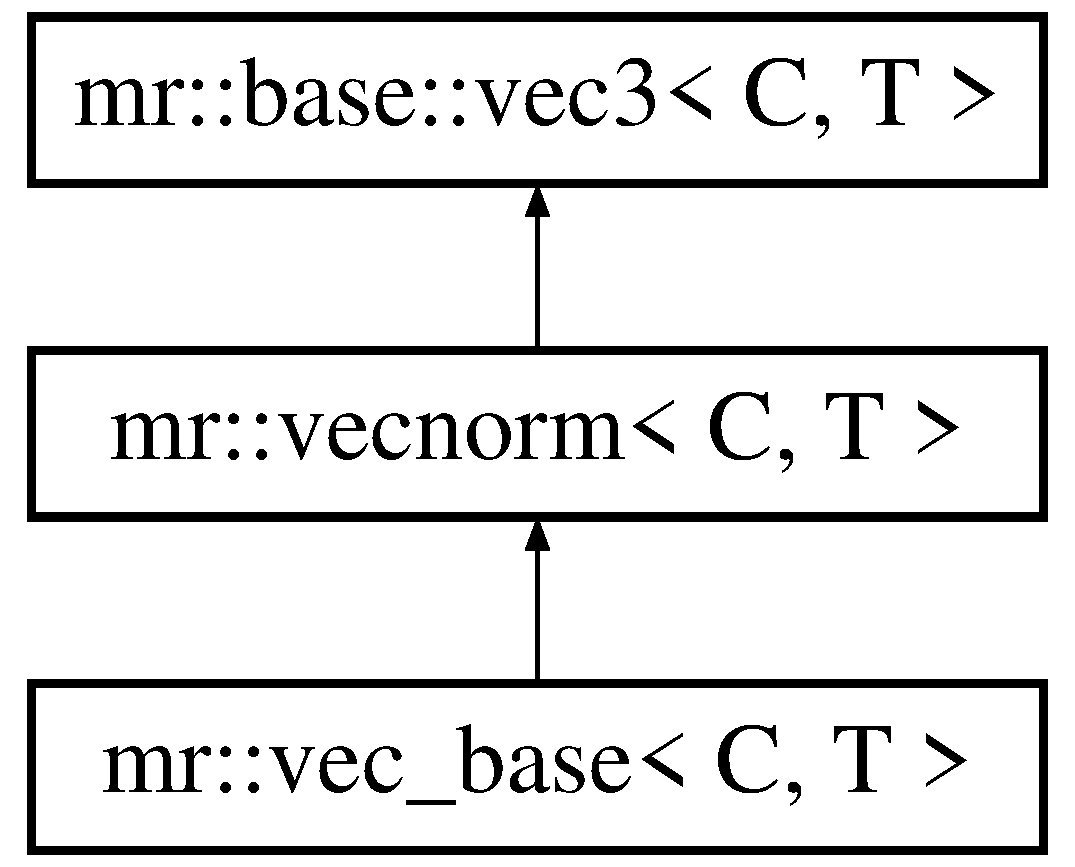
\includegraphics[height=3cm]{structmr_1_1vec__base}
\end{center}
\end{figure}
\subsection*{Public Types}
\begin{CompactItemize}
\item 
typedef {\bf vec\_\-base}$<$ C, T $>$ {\bf self}
\end{CompactItemize}
\subsection*{Public Member Functions}
\begin{CompactItemize}
\item 
void {\bf to\-Tangent} (const mi\-State $\ast$const state, const int idx=0)
\item 
void {\bf to\-Object} (const mi\-State $\ast$const state)
\item 
void {\bf to\-World} (const mi\-State $\ast$const state)
\item 
void {\bf to\-Camera} (const mi\-State $\ast$const state)
\item 
void {\bf to\-Raster} (const mi\-State $\ast$const state)
\item 
void {\bf to\-NDC} (const mi\-State $\ast$const state)
\item 
void {\bf to\-Light} (const mi\-State $\ast$const state)
\item 
void {\bf from\-Tangent} (const mi\-State $\ast$const state, const int idx=0)
\item 
void {\bf from\-Object} (const mi\-State $\ast$const state)
\item 
void {\bf from\-World} (const mi\-State $\ast$const state)
\item 
void {\bf from\-Camera} (const mi\-State $\ast$const state)
\item 
void {\bf from\-Raster} (const mi\-State $\ast$const state)
\item 
void {\bf from\-Light} (const mi\-State $\ast$const state)
\item 
void {\bf to} (const mi\-State $\ast$const state, const {\bf space::type} to\-Space)
\item 
void {\bf from} (const mi\-State $\ast$const state, const {\bf space::type} from\-Space)
\item 
void {\bf transform} (const mi\-State $\ast$const state, const {\bf space::type} from\-Space, const {\bf space::type} to\-Space)
\item 
{\bf self} {\bf inverse} () const 
\item 
{\bf self} {\bf operator-} () const 
\item 
{\bf self} {\bf normalized} () const 
\item 
{\bf self} {\bf normalized\-Fast} () const 
\item 
{\bf self} {\bf operator $\ast$} (const mi\-Matrix m) const 
\item 
{\bf self} {\bf operator $\ast$} (const {\bf matrix} \&m) const 
\end{CompactItemize}
\begin{Indent}{\bf Constructors}\par
\begin{CompactItemize}
\item 
{\bf vec\_\-base} ()
\item 
template$<$class X, class Y, class Oper$>$ {\bf vec\_\-base} (const {\bf base::exp}$<$ X, Y, Oper $>$ \&e)
\item 
{\bf vec\_\-base} ({\bf k\-No\-Construct})
\begin{CompactList}\small\item\em Empty and fast constructor. x,y,z are undefined. \item\end{CompactList}\item 
{\bf vec\_\-base} (const C \&b)
\begin{CompactList}\small\item\em Constructor from a similar mi\-Vector. \item\end{CompactList}\item 
{\bf vec\_\-base} (const T b)
\begin{CompactList}\small\item\em Constructor from a single value. \item\end{CompactList}\item 
{\bf vec\_\-base} (const T xx, const T yy, const T zz)
\begin{CompactList}\small\item\em Constructor from three values. \item\end{CompactList}\item 
{\bf vec\_\-base} (const mi\-State $\ast$const state, const {\bf space::type} from\-Space, const C \&v)
\begin{CompactList}\small\item\em Constructor from another mi\-Vector, assuming it comes from a space. \item\end{CompactList}\item 
{\bf vec\_\-base} (const mi\-State $\ast$const state, const {\bf space::type} from\-Space, const T xx, const T yy, const T zz)
\begin{CompactList}\small\item\em Constructor from 3 values, assuming they are defined in some space. \item\end{CompactList}\end{CompactItemize}
\end{Indent}
\begin{Indent}{\bf Copy Constructor}\par
\begin{CompactItemize}
\item 
{\bf vec\_\-base} (const {\bf self} \&b)
\end{CompactItemize}
\end{Indent}
\begin{Indent}{\bf Assignment}\par
\begin{CompactItemize}
\item 
template$<$class X, class Y, class Oper$>$ const {\bf self} \& {\bf operator=} (const {\bf base::exp}$<$ X, Y, Oper $>$ \&e)
\begin{CompactList}\small\item\em Handle assignment when we deal with a chained operation. \item\end{CompactList}\item 
const {\bf self} \& {\bf operator=} (const {\bf self} \&b)
\begin{CompactList}\small\item\em Assignment of similar object. \item\end{CompactList}\item 
const {\bf self} \& {\bf operator=} (const C \&b)
\begin{CompactList}\small\item\em Assignemnt of base class object. \item\end{CompactList}\item 
const {\bf self} \& {\bf operator=} (const T b)
\begin{CompactList}\small\item\em Assignment of base type. \item\end{CompactList}\end{CompactItemize}
\end{Indent}
\begin{Indent}{\bf Cross product}\par
\begin{CompactItemize}
\item 
template$<$class X, class Y, class Oper$>$ const {\bf self} \& {\bf operator$^\wedge$=} (const {\bf base::exp}$<$ X, Y, Oper $>$ \&b)
\item 
const {\bf self} \& {\bf operator$^\wedge$=} (const mi\-Vector \&b)
\item 
template$<$typename X$>$ const {\bf self} \& {\bf cross} (const X \&b)
\item 
template$<$class X, class Y, class Oper$>$ {\bf self} {\bf operator$^\wedge$} (const {\bf base::exp}$<$ X, Y, Oper $>$ \&b) const 
\item 
{\bf self} {\bf operator$^\wedge$} (const mi\-Vector \&b) const 
\end{CompactItemize}
\end{Indent}
\begin{Indent}{\bf REFERENCE OPERATORS (MODIFY IN PLACE)}\par
\begin{CompactItemize}
\item 
const {\bf self} \& {\bf operator $\ast$=} (const T b)
\item 
const {\bf self} \& {\bf operator $\ast$=} (const C \&b)
\item 
const {\bf self} \& {\bf operator $\ast$=} (const mi\-Matrix a)
\item 
const {\bf self} \& {\bf operator $\ast$=} (const {\bf matrix} \&m)
\end{CompactItemize}
\end{Indent}
\subsection*{Static Public Attributes}
\begin{CompactItemize}
\item 
{\bf vec\_\-base}$<$ C, T $>$ {\bf k\-Null}
\item 
{\bf vec\_\-base}$<$ C, T $>$ {\bf k\-Axis\-X}
\item 
{\bf vec\_\-base}$<$ C, T $>$ {\bf k\-Axis\-Y}
\item 
{\bf vec\_\-base}$<$ C, T $>$ {\bf k\-Axis\-Z}
\item 
{\bf vec\_\-base}$<$ C, T $>$ {\bf k\-Unit\-Scale}
\end{CompactItemize}
\subsubsection*{template$<$class C, typename T$>$ struct mr::vec\_\-base$<$ C, T $>$}



\subsection{Member Typedef Documentation}
\index{mr::vec_base@{mr::vec\_\-base}!self@{self}}
\index{self@{self}!mr::vec_base@{mr::vec\_\-base}}
\subsubsection{\setlength{\rightskip}{0pt plus 5cm}template$<$class C, typename T$>$ typedef {\bf vec\_\-base}$<$ C, T $>$ {\bf mr::vec\_\-base}$<$ C, T $>$::{\bf self}}\label{structmr_1_1vec__base_w0}




Reimplemented from {\bf mr::vecnorm$<$ C, T $>$} {\rm (p.\,\pageref{structmr_1_1vecnorm_w0})}.

\subsection{Constructor \& Destructor Documentation}
\index{mr::vec_base@{mr::vec\_\-base}!vec_base@{vec\_\-base}}
\index{vec_base@{vec\_\-base}!mr::vec_base@{mr::vec\_\-base}}
\subsubsection{\setlength{\rightskip}{0pt plus 5cm}template$<$class C, typename T$>$ {\bf mr::vec\_\-base}$<$ C, T $>$::{\bf vec\_\-base} ()\hspace{0.3cm}{\tt  [inline]}}\label{structmr_1_1vec__base_z58_0}


\index{mr::vec_base@{mr::vec\_\-base}!vec_base@{vec\_\-base}}
\index{vec_base@{vec\_\-base}!mr::vec_base@{mr::vec\_\-base}}
\subsubsection{\setlength{\rightskip}{0pt plus 5cm}template$<$class C, typename T$>$ template$<$class X, class Y, class Oper$>$ {\bf mr::vec\_\-base}$<$ C, T $>$::{\bf vec\_\-base} (const {\bf base::exp}$<$ X, Y, Oper $>$ \& {\em e})\hspace{0.3cm}{\tt  [inline]}}\label{structmr_1_1vec__base_z58_1}


\index{mr::vec_base@{mr::vec\_\-base}!vec_base@{vec\_\-base}}
\index{vec_base@{vec\_\-base}!mr::vec_base@{mr::vec\_\-base}}
\subsubsection{\setlength{\rightskip}{0pt plus 5cm}template$<$class C, typename T$>$ {\bf mr::vec\_\-base}$<$ C, T $>$::{\bf vec\_\-base} ({\bf k\-No\-Construct})\hspace{0.3cm}{\tt  [inline]}}\label{structmr_1_1vec__base_z58_2}


Empty and fast constructor. x,y,z are undefined. 

\index{mr::vec_base@{mr::vec\_\-base}!vec_base@{vec\_\-base}}
\index{vec_base@{vec\_\-base}!mr::vec_base@{mr::vec\_\-base}}
\subsubsection{\setlength{\rightskip}{0pt plus 5cm}template$<$class C, typename T$>$ {\bf mr::vec\_\-base}$<$ C, T $>$::{\bf vec\_\-base} (const C \& {\em b})\hspace{0.3cm}{\tt  [inline]}}\label{structmr_1_1vec__base_z58_3}


Constructor from a similar mi\-Vector. 

\index{mr::vec_base@{mr::vec\_\-base}!vec_base@{vec\_\-base}}
\index{vec_base@{vec\_\-base}!mr::vec_base@{mr::vec\_\-base}}
\subsubsection{\setlength{\rightskip}{0pt plus 5cm}template$<$class C, typename T$>$ {\bf mr::vec\_\-base}$<$ C, T $>$::{\bf vec\_\-base} (const T {\em b})\hspace{0.3cm}{\tt  [inline]}}\label{structmr_1_1vec__base_z58_4}


Constructor from a single value. 

\index{mr::vec_base@{mr::vec\_\-base}!vec_base@{vec\_\-base}}
\index{vec_base@{vec\_\-base}!mr::vec_base@{mr::vec\_\-base}}
\subsubsection{\setlength{\rightskip}{0pt plus 5cm}template$<$class C, typename T$>$ {\bf mr::vec\_\-base}$<$ C, T $>$::{\bf vec\_\-base} (const T {\em xx}, const T {\em yy}, const T {\em zz})\hspace{0.3cm}{\tt  [inline]}}\label{structmr_1_1vec__base_z58_5}


Constructor from three values. 

\index{mr::vec_base@{mr::vec\_\-base}!vec_base@{vec\_\-base}}
\index{vec_base@{vec\_\-base}!mr::vec_base@{mr::vec\_\-base}}
\subsubsection{\setlength{\rightskip}{0pt plus 5cm}template$<$class C, typename T$>$ {\bf mr::vec\_\-base}$<$ C, T $>$::{\bf vec\_\-base} (const mi\-State $\ast$const {\em state}, const {\bf space::type} {\em from\-Space}, const C \& {\em v})\hspace{0.3cm}{\tt  [inline]}}\label{structmr_1_1vec__base_z58_6}


Constructor from another mi\-Vector, assuming it comes from a space. 

\index{mr::vec_base@{mr::vec\_\-base}!vec_base@{vec\_\-base}}
\index{vec_base@{vec\_\-base}!mr::vec_base@{mr::vec\_\-base}}
\subsubsection{\setlength{\rightskip}{0pt plus 5cm}template$<$class C, typename T$>$ {\bf mr::vec\_\-base}$<$ C, T $>$::{\bf vec\_\-base} (const mi\-State $\ast$const {\em state}, const {\bf space::type} {\em from\-Space}, const T {\em xx}, const T {\em yy}, const T {\em zz})\hspace{0.3cm}{\tt  [inline]}}\label{structmr_1_1vec__base_z58_7}


Constructor from 3 values, assuming they are defined in some space. 

\index{mr::vec_base@{mr::vec\_\-base}!vec_base@{vec\_\-base}}
\index{vec_base@{vec\_\-base}!mr::vec_base@{mr::vec\_\-base}}
\subsubsection{\setlength{\rightskip}{0pt plus 5cm}template$<$class C, typename T$>$ {\bf mr::vec\_\-base}$<$ C, T $>$::{\bf vec\_\-base} (const {\bf self} \& {\em b})\hspace{0.3cm}{\tt  [inline]}}\label{structmr_1_1vec__base_z59_0}




\subsection{Member Function Documentation}
\index{mr::vec_base@{mr::vec\_\-base}!cross@{cross}}
\index{cross@{cross}!mr::vec_base@{mr::vec\_\-base}}
\subsubsection{\setlength{\rightskip}{0pt plus 5cm}template$<$class C, typename T$>$ template$<$typename X$>$ const {\bf self}\& {\bf mr::vec\_\-base}$<$ C, T $>$::cross (const X \& {\em b})\hspace{0.3cm}{\tt  [inline]}}\label{structmr_1_1vec__base_z62_2}


\index{mr::vec_base@{mr::vec\_\-base}!from@{from}}
\index{from@{from}!mr::vec_base@{mr::vec\_\-base}}
\subsubsection{\setlength{\rightskip}{0pt plus 5cm}template$<$class C, typename T$>$ void {\bf mr::vec\_\-base}$<$ C, T $>$::from (const mi\-State $\ast$const {\em state}, const {\bf space::type} {\em from\-Space})\hspace{0.3cm}{\tt  [inline]}}\label{structmr_1_1vec__base_a14}


\index{mr::vec_base@{mr::vec\_\-base}!fromCamera@{fromCamera}}
\index{fromCamera@{fromCamera}!mr::vec_base@{mr::vec\_\-base}}
\subsubsection{\setlength{\rightskip}{0pt plus 5cm}template$<$class C, typename T$>$ void {\bf mr::vec\_\-base}$<$ C, T $>$::from\-Camera (const mi\-State $\ast$const {\em state})\hspace{0.3cm}{\tt  [inline]}}\label{structmr_1_1vec__base_a10}


\index{mr::vec_base@{mr::vec\_\-base}!fromLight@{fromLight}}
\index{fromLight@{fromLight}!mr::vec_base@{mr::vec\_\-base}}
\subsubsection{\setlength{\rightskip}{0pt plus 5cm}template$<$class C, typename T$>$ void {\bf mr::vec\_\-base}$<$ C, T $>$::from\-Light (const mi\-State $\ast$const {\em state})\hspace{0.3cm}{\tt  [inline]}}\label{structmr_1_1vec__base_a12}


\index{mr::vec_base@{mr::vec\_\-base}!fromObject@{fromObject}}
\index{fromObject@{fromObject}!mr::vec_base@{mr::vec\_\-base}}
\subsubsection{\setlength{\rightskip}{0pt plus 5cm}template$<$class C, typename T$>$ void {\bf mr::vec\_\-base}$<$ C, T $>$::from\-Object (const mi\-State $\ast$const {\em state})\hspace{0.3cm}{\tt  [inline]}}\label{structmr_1_1vec__base_a8}


\index{mr::vec_base@{mr::vec\_\-base}!fromRaster@{fromRaster}}
\index{fromRaster@{fromRaster}!mr::vec_base@{mr::vec\_\-base}}
\subsubsection{\setlength{\rightskip}{0pt plus 5cm}template$<$class C, typename T$>$ void {\bf mr::vec\_\-base}$<$ C, T $>$::from\-Raster (const mi\-State $\ast$const {\em state})\hspace{0.3cm}{\tt  [inline]}}\label{structmr_1_1vec__base_a11}


\index{mr::vec_base@{mr::vec\_\-base}!fromTangent@{fromTangent}}
\index{fromTangent@{fromTangent}!mr::vec_base@{mr::vec\_\-base}}
\subsubsection{\setlength{\rightskip}{0pt plus 5cm}template$<$class C, typename T$>$ void {\bf mr::vec\_\-base}$<$ C, T $>$::from\-Tangent (const mi\-State $\ast$const {\em state}, const int {\em idx} = 0)\hspace{0.3cm}{\tt  [inline]}}\label{structmr_1_1vec__base_a7}


\index{mr::vec_base@{mr::vec\_\-base}!fromWorld@{fromWorld}}
\index{fromWorld@{fromWorld}!mr::vec_base@{mr::vec\_\-base}}
\subsubsection{\setlength{\rightskip}{0pt plus 5cm}template$<$class C, typename T$>$ void {\bf mr::vec\_\-base}$<$ C, T $>$::from\-World (const mi\-State $\ast$const {\em state})\hspace{0.3cm}{\tt  [inline]}}\label{structmr_1_1vec__base_a9}


\index{mr::vec_base@{mr::vec\_\-base}!inverse@{inverse}}
\index{inverse@{inverse}!mr::vec_base@{mr::vec\_\-base}}
\subsubsection{\setlength{\rightskip}{0pt plus 5cm}template$<$class C, typename T$>$ {\bf self} {\bf mr::vec\_\-base}$<$ C, T $>$::inverse () const\hspace{0.3cm}{\tt  [inline]}}\label{structmr_1_1vec__base_a16}


\index{mr::vec_base@{mr::vec\_\-base}!normalized@{normalized}}
\index{normalized@{normalized}!mr::vec_base@{mr::vec\_\-base}}
\subsubsection{\setlength{\rightskip}{0pt plus 5cm}template$<$class C, typename T$>$ {\bf self} {\bf mr::vec\_\-base}$<$ C, T $>$::normalized () const\hspace{0.3cm}{\tt  [inline]}}\label{structmr_1_1vec__base_a18}


\index{mr::vec_base@{mr::vec\_\-base}!normalizedFast@{normalizedFast}}
\index{normalizedFast@{normalizedFast}!mr::vec_base@{mr::vec\_\-base}}
\subsubsection{\setlength{\rightskip}{0pt plus 5cm}template$<$class C, typename T$>$ {\bf self} {\bf mr::vec\_\-base}$<$ C, T $>$::normalized\-Fast () const\hspace{0.3cm}{\tt  [inline]}}\label{structmr_1_1vec__base_a19}


\index{mr::vec_base@{mr::vec\_\-base}!operator *@{operator $\ast$}}
\index{operator *@{operator $\ast$}!mr::vec_base@{mr::vec\_\-base}}
\subsubsection{\setlength{\rightskip}{0pt plus 5cm}template$<$class C, typename T$>$ {\bf self} {\bf mr::vec\_\-base}$<$ C, T $>$::operator $\ast$ (const {\bf matrix} \& {\em m}) const\hspace{0.3cm}{\tt  [inline]}}\label{structmr_1_1vec__base_a21}


\index{mr::vec_base@{mr::vec\_\-base}!operator *@{operator $\ast$}}
\index{operator *@{operator $\ast$}!mr::vec_base@{mr::vec\_\-base}}
\subsubsection{\setlength{\rightskip}{0pt plus 5cm}template$<$class C, typename T$>$ {\bf self} {\bf mr::vec\_\-base}$<$ C, T $>$::operator $\ast$ (const mi\-Matrix {\em m}) const\hspace{0.3cm}{\tt  [inline]}}\label{structmr_1_1vec__base_a20}


\index{mr::vec_base@{mr::vec\_\-base}!operator *=@{operator $\ast$=}}
\index{operator *=@{operator $\ast$=}!mr::vec_base@{mr::vec\_\-base}}
\subsubsection{\setlength{\rightskip}{0pt plus 5cm}template$<$class C, typename T$>$ const {\bf self}\& {\bf mr::vec\_\-base}$<$ C, T $>$::operator $\ast$= (const {\bf matrix} \& {\em m})\hspace{0.3cm}{\tt  [inline]}}\label{structmr_1_1vec__base_z64_3}


\index{mr::vec_base@{mr::vec\_\-base}!operator *=@{operator $\ast$=}}
\index{operator *=@{operator $\ast$=}!mr::vec_base@{mr::vec\_\-base}}
\subsubsection{\setlength{\rightskip}{0pt plus 5cm}template$<$class C, typename T$>$ const {\bf self}\& {\bf mr::vec\_\-base}$<$ C, T $>$::operator $\ast$= (const mi\-Matrix {\em a})\hspace{0.3cm}{\tt  [inline]}}\label{structmr_1_1vec__base_z64_2}


\index{mr::vec_base@{mr::vec\_\-base}!operator *=@{operator $\ast$=}}
\index{operator *=@{operator $\ast$=}!mr::vec_base@{mr::vec\_\-base}}
\subsubsection{\setlength{\rightskip}{0pt plus 5cm}template$<$class C, typename T$>$ const {\bf self}\& {\bf mr::vec\_\-base}$<$ C, T $>$::operator $\ast$= (const C \& {\em b})\hspace{0.3cm}{\tt  [inline]}}\label{structmr_1_1vec__base_z64_1}




Reimplemented from {\bf mr::base::vec3$<$ C, T $>$} {\rm (p.\,\pageref{structmr_1_1base_1_1vec3_z40_8})}.\index{mr::vec_base@{mr::vec\_\-base}!operator *=@{operator $\ast$=}}
\index{operator *=@{operator $\ast$=}!mr::vec_base@{mr::vec\_\-base}}
\subsubsection{\setlength{\rightskip}{0pt plus 5cm}template$<$class C, typename T$>$ const {\bf self}\& {\bf mr::vec\_\-base}$<$ C, T $>$::operator $\ast$= (const T {\em b})\hspace{0.3cm}{\tt  [inline]}}\label{structmr_1_1vec__base_z64_0}




Reimplemented from {\bf mr::base::vec3$<$ C, T $>$} {\rm (p.\,\pageref{structmr_1_1base_1_1vec3_z40_7})}.\index{mr::vec_base@{mr::vec\_\-base}!operator-@{operator-}}
\index{operator-@{operator-}!mr::vec_base@{mr::vec\_\-base}}
\subsubsection{\setlength{\rightskip}{0pt plus 5cm}template$<$class C, typename T$>$ {\bf self} {\bf mr::vec\_\-base}$<$ C, T $>$::operator- () const\hspace{0.3cm}{\tt  [inline]}}\label{structmr_1_1vec__base_a17}


\index{mr::vec_base@{mr::vec\_\-base}!operator=@{operator=}}
\index{operator=@{operator=}!mr::vec_base@{mr::vec\_\-base}}
\subsubsection{\setlength{\rightskip}{0pt plus 5cm}template$<$class C, typename T$>$ const {\bf self}\& {\bf mr::vec\_\-base}$<$ C, T $>$::operator= (const T {\em b})\hspace{0.3cm}{\tt  [inline]}}\label{structmr_1_1vec__base_z60_3}


Assignment of base type. 



Reimplemented from {\bf mr::base::vec3$<$ C, T $>$} {\rm (p.\,\pageref{structmr_1_1base_1_1vec3_z36_3})}.\index{mr::vec_base@{mr::vec\_\-base}!operator=@{operator=}}
\index{operator=@{operator=}!mr::vec_base@{mr::vec\_\-base}}
\subsubsection{\setlength{\rightskip}{0pt plus 5cm}template$<$class C, typename T$>$ const {\bf self}\& {\bf mr::vec\_\-base}$<$ C, T $>$::operator= (const C \& {\em b})\hspace{0.3cm}{\tt  [inline]}}\label{structmr_1_1vec__base_z60_2}


Assignemnt of base class object. 



Reimplemented from {\bf mr::base::vec3$<$ C, T $>$} {\rm (p.\,\pageref{structmr_1_1base_1_1vec3_z36_2})}.\index{mr::vec_base@{mr::vec\_\-base}!operator=@{operator=}}
\index{operator=@{operator=}!mr::vec_base@{mr::vec\_\-base}}
\subsubsection{\setlength{\rightskip}{0pt plus 5cm}template$<$class C, typename T$>$ const {\bf self}\& {\bf mr::vec\_\-base}$<$ C, T $>$::operator= (const {\bf self} \& {\em b})\hspace{0.3cm}{\tt  [inline]}}\label{structmr_1_1vec__base_z60_1}


Assignment of similar object. 



Reimplemented from {\bf mr::base::vec3$<$ C, T $>$} {\rm (p.\,\pageref{structmr_1_1base_1_1vec3_z36_1})}.\index{mr::vec_base@{mr::vec\_\-base}!operator=@{operator=}}
\index{operator=@{operator=}!mr::vec_base@{mr::vec\_\-base}}
\subsubsection{\setlength{\rightskip}{0pt plus 5cm}template$<$class C, typename T$>$ template$<$class X, class Y, class Oper$>$ const {\bf self}\& {\bf mr::vec\_\-base}$<$ C, T $>$::operator= (const {\bf base::exp}$<$ X, Y, Oper $>$ \& {\em e})\hspace{0.3cm}{\tt  [inline]}}\label{structmr_1_1vec__base_z60_0}


Handle assignment when we deal with a chained operation. 



Reimplemented from {\bf mr::base::vec3$<$ C, T $>$} {\rm (p.\,\pageref{structmr_1_1base_1_1vec3_z36_0})}.\index{mr::vec_base@{mr::vec\_\-base}!operator^@{operator$^\wedge$}}
\index{operator^@{operator$^\wedge$}!mr::vec_base@{mr::vec\_\-base}}
\subsubsection{\setlength{\rightskip}{0pt plus 5cm}template$<$class C, typename T$>$ {\bf self} {\bf mr::vec\_\-base}$<$ C, T $>$::operator$^\wedge$ (const mi\-Vector \& {\em b}) const\hspace{0.3cm}{\tt  [inline]}}\label{structmr_1_1vec__base_z62_4}


\index{mr::vec_base@{mr::vec\_\-base}!operator^@{operator$^\wedge$}}
\index{operator^@{operator$^\wedge$}!mr::vec_base@{mr::vec\_\-base}}
\subsubsection{\setlength{\rightskip}{0pt plus 5cm}template$<$class C, typename T$>$ template$<$class X, class Y, class Oper$>$ {\bf self} {\bf mr::vec\_\-base}$<$ C, T $>$::operator$^\wedge$ (const {\bf base::exp}$<$ X, Y, Oper $>$ \& {\em b}) const\hspace{0.3cm}{\tt  [inline]}}\label{structmr_1_1vec__base_z62_3}


\index{mr::vec_base@{mr::vec\_\-base}!operator^=@{operator$^\wedge$=}}
\index{operator^=@{operator$^\wedge$=}!mr::vec_base@{mr::vec\_\-base}}
\subsubsection{\setlength{\rightskip}{0pt plus 5cm}template$<$class C, typename T$>$ const {\bf self}\& {\bf mr::vec\_\-base}$<$ C, T $>$::operator$^\wedge$= (const mi\-Vector \& {\em b})\hspace{0.3cm}{\tt  [inline]}}\label{structmr_1_1vec__base_z62_1}


\index{mr::vec_base@{mr::vec\_\-base}!operator^=@{operator$^\wedge$=}}
\index{operator^=@{operator$^\wedge$=}!mr::vec_base@{mr::vec\_\-base}}
\subsubsection{\setlength{\rightskip}{0pt plus 5cm}template$<$class C, typename T$>$ template$<$class X, class Y, class Oper$>$ const {\bf self}\& {\bf mr::vec\_\-base}$<$ C, T $>$::operator$^\wedge$= (const {\bf base::exp}$<$ X, Y, Oper $>$ \& {\em b})\hspace{0.3cm}{\tt  [inline]}}\label{structmr_1_1vec__base_z62_0}


\index{mr::vec_base@{mr::vec\_\-base}!to@{to}}
\index{to@{to}!mr::vec_base@{mr::vec\_\-base}}
\subsubsection{\setlength{\rightskip}{0pt plus 5cm}template$<$class C, typename T$>$ void {\bf mr::vec\_\-base}$<$ C, T $>$::to (const mi\-State $\ast$const {\em state}, const {\bf space::type} {\em to\-Space})\hspace{0.3cm}{\tt  [inline]}}\label{structmr_1_1vec__base_a13}


\index{mr::vec_base@{mr::vec\_\-base}!toCamera@{toCamera}}
\index{toCamera@{toCamera}!mr::vec_base@{mr::vec\_\-base}}
\subsubsection{\setlength{\rightskip}{0pt plus 5cm}template$<$class C, typename T$>$ void {\bf mr::vec\_\-base}$<$ C, T $>$::to\-Camera (const mi\-State $\ast$const {\em state})\hspace{0.3cm}{\tt  [inline]}}\label{structmr_1_1vec__base_a3}


\index{mr::vec_base@{mr::vec\_\-base}!toLight@{toLight}}
\index{toLight@{toLight}!mr::vec_base@{mr::vec\_\-base}}
\subsubsection{\setlength{\rightskip}{0pt plus 5cm}template$<$class C, typename T$>$ void {\bf mr::vec\_\-base}$<$ C, T $>$::to\-Light (const mi\-State $\ast$const {\em state})\hspace{0.3cm}{\tt  [inline]}}\label{structmr_1_1vec__base_a6}


\index{mr::vec_base@{mr::vec\_\-base}!toNDC@{toNDC}}
\index{toNDC@{toNDC}!mr::vec_base@{mr::vec\_\-base}}
\subsubsection{\setlength{\rightskip}{0pt plus 5cm}template$<$class C, typename T$>$ void {\bf mr::vec\_\-base}$<$ C, T $>$::to\-NDC (const mi\-State $\ast$const {\em state})\hspace{0.3cm}{\tt  [inline]}}\label{structmr_1_1vec__base_a5}


\index{mr::vec_base@{mr::vec\_\-base}!toObject@{toObject}}
\index{toObject@{toObject}!mr::vec_base@{mr::vec\_\-base}}
\subsubsection{\setlength{\rightskip}{0pt plus 5cm}template$<$class C, typename T$>$ void {\bf mr::vec\_\-base}$<$ C, T $>$::to\-Object (const mi\-State $\ast$const {\em state})\hspace{0.3cm}{\tt  [inline]}}\label{structmr_1_1vec__base_a1}


\index{mr::vec_base@{mr::vec\_\-base}!toRaster@{toRaster}}
\index{toRaster@{toRaster}!mr::vec_base@{mr::vec\_\-base}}
\subsubsection{\setlength{\rightskip}{0pt plus 5cm}template$<$class C, typename T$>$ void {\bf mr::vec\_\-base}$<$ C, T $>$::to\-Raster (const mi\-State $\ast$const {\em state})\hspace{0.3cm}{\tt  [inline]}}\label{structmr_1_1vec__base_a4}


\index{mr::vec_base@{mr::vec\_\-base}!toTangent@{toTangent}}
\index{toTangent@{toTangent}!mr::vec_base@{mr::vec\_\-base}}
\subsubsection{\setlength{\rightskip}{0pt plus 5cm}template$<$class C, typename T$>$ void {\bf mr::vec\_\-base}$<$ C, T $>$::to\-Tangent (const mi\-State $\ast$const {\em state}, const int {\em idx} = 0)\hspace{0.3cm}{\tt  [inline]}}\label{structmr_1_1vec__base_a0}


\index{mr::vec_base@{mr::vec\_\-base}!toWorld@{toWorld}}
\index{toWorld@{toWorld}!mr::vec_base@{mr::vec\_\-base}}
\subsubsection{\setlength{\rightskip}{0pt plus 5cm}template$<$class C, typename T$>$ void {\bf mr::vec\_\-base}$<$ C, T $>$::to\-World (const mi\-State $\ast$const {\em state})\hspace{0.3cm}{\tt  [inline]}}\label{structmr_1_1vec__base_a2}


\index{mr::vec_base@{mr::vec\_\-base}!transform@{transform}}
\index{transform@{transform}!mr::vec_base@{mr::vec\_\-base}}
\subsubsection{\setlength{\rightskip}{0pt plus 5cm}template$<$class C, typename T$>$ void {\bf mr::vec\_\-base}$<$ C, T $>$::transform (const mi\-State $\ast$const {\em state}, const {\bf space::type} {\em from\-Space}, const {\bf space::type} {\em to\-Space})\hspace{0.3cm}{\tt  [inline]}}\label{structmr_1_1vec__base_a15}




\subsection{Member Data Documentation}
\index{mr::vec_base@{mr::vec\_\-base}!kAxisX@{kAxisX}}
\index{kAxisX@{kAxisX}!mr::vec_base@{mr::vec\_\-base}}
\subsubsection{\setlength{\rightskip}{0pt plus 5cm}template$<$class C, typename T$>$ {\bf vec\_\-base}$<$ C, T $>$ {\bf mr::vec\_\-base}$<$ C, T $>$::{\bf k\-Axis\-X}\hspace{0.3cm}{\tt  [static]}}\label{structmr_1_1vec__base_s1}


\index{mr::vec_base@{mr::vec\_\-base}!kAxisY@{kAxisY}}
\index{kAxisY@{kAxisY}!mr::vec_base@{mr::vec\_\-base}}
\subsubsection{\setlength{\rightskip}{0pt plus 5cm}template$<$class C, typename T$>$ {\bf vec\_\-base}$<$ C, T $>$ {\bf mr::vec\_\-base}$<$ C, T $>$::{\bf k\-Axis\-Y}\hspace{0.3cm}{\tt  [static]}}\label{structmr_1_1vec__base_s2}


\index{mr::vec_base@{mr::vec\_\-base}!kAxisZ@{kAxisZ}}
\index{kAxisZ@{kAxisZ}!mr::vec_base@{mr::vec\_\-base}}
\subsubsection{\setlength{\rightskip}{0pt plus 5cm}template$<$class C, typename T$>$ {\bf vec\_\-base}$<$ C, T $>$ {\bf mr::vec\_\-base}$<$ C, T $>$::{\bf k\-Axis\-Z}\hspace{0.3cm}{\tt  [static]}}\label{structmr_1_1vec__base_s3}


\index{mr::vec_base@{mr::vec\_\-base}!kNull@{kNull}}
\index{kNull@{kNull}!mr::vec_base@{mr::vec\_\-base}}
\subsubsection{\setlength{\rightskip}{0pt plus 5cm}template$<$class C, typename T$>$ {\bf vec\_\-base}$<$ C, T $>$ {\bf mr::vec\_\-base}$<$ C, T $>$::{\bf k\-Null}\hspace{0.3cm}{\tt  [static]}}\label{structmr_1_1vec__base_s0}


\index{mr::vec_base@{mr::vec\_\-base}!kUnitScale@{kUnitScale}}
\index{kUnitScale@{kUnitScale}!mr::vec_base@{mr::vec\_\-base}}
\subsubsection{\setlength{\rightskip}{0pt plus 5cm}template$<$class C, typename T$>$ {\bf vec\_\-base}$<$ C, T $>$ {\bf mr::vec\_\-base}$<$ C, T $>$::{\bf k\-Unit\-Scale}\hspace{0.3cm}{\tt  [static]}}\label{structmr_1_1vec__base_s4}




The documentation for this struct was generated from the following files:\begin{CompactItemize}
\item 
{\bf mr\-Vector.h}\item 
{\bf mr\-Derivs.h}\end{CompactItemize}

\section{mr::base::vecarg$<$ ta\_\-a $>$ Class Template Reference}
\label{classmr_1_1base_1_1vecarg}\index{mr::base::vecarg@{mr::base::vecarg}}
{\tt \#include $<$mr\-Base.h$>$}

\subsection*{Public Member Functions}
\begin{CompactItemize}
\item 
{\bf vecarg} (const ta\_\-a \&A)
\item 
const double {\bf Evaluate} (const unsigned short i) const 
\end{CompactItemize}
\subsubsection*{template$<$typename ta\_\-a$>$ class mr::base::vecarg$<$ ta\_\-a $>$}



\subsection{Constructor \& Destructor Documentation}
\index{mr::base::vecarg@{mr::base::vecarg}!vecarg@{vecarg}}
\index{vecarg@{vecarg}!mr::base::vecarg@{mr::base::vecarg}}
\subsubsection{\setlength{\rightskip}{0pt plus 5cm}template$<$typename ta\_\-a$>$ {\bf mr::base::vecarg}$<$ ta\_\-a $>$::{\bf vecarg} (const ta\_\-a \& {\em A})\hspace{0.3cm}{\tt  [inline]}}\label{classmr_1_1base_1_1vecarg_a0}




\subsection{Member Function Documentation}
\index{mr::base::vecarg@{mr::base::vecarg}!Evaluate@{Evaluate}}
\index{Evaluate@{Evaluate}!mr::base::vecarg@{mr::base::vecarg}}
\subsubsection{\setlength{\rightskip}{0pt plus 5cm}template$<$typename ta\_\-a$>$ const double {\bf mr::base::vecarg}$<$ ta\_\-a $>$::Evaluate (const unsigned short {\em i}) const\hspace{0.3cm}{\tt  [inline]}}\label{classmr_1_1base_1_1vecarg_a1}




The documentation for this class was generated from the following file:\begin{CompactItemize}
\item 
{\bf mr\-Base.h}\end{CompactItemize}

\section{mr::base::vecarg$<$ const double $>$ Class Template Reference}
\label{classmr_1_1base_1_1vecarg_3_01const_01double_01_4}\index{mr::base::vecarg< const double >@{mr::base::vecarg$<$ const double $>$}}
{\tt \#include $<$mr\-Base.h$>$}

\subsection*{Public Member Functions}
\begin{CompactItemize}
\item 
{\bf vecarg} (const double \&A)
\item 
const double {\bf Evaluate} (const unsigned short i) const 
\end{CompactItemize}
\subsubsection*{template$<$$>$ class mr::base::vecarg$<$ const double $>$}



\subsection{Member Function Documentation}
\index{mr::base::vecarg< const double >@{mr::base::vecarg$<$ const double $>$}!Evaluate@{Evaluate}}
\index{Evaluate@{Evaluate}!mr::base::vecarg< const double >@{mr::base::vecarg$<$ const double $>$}}
\subsubsection{\setlength{\rightskip}{0pt plus 5cm}const double {\bf mr::base::vecarg}$<$ const double $>$::Evaluate (const unsigned short {\em i}) const\hspace{0.3cm}{\tt  [inline]}}\label{classmr_1_1base_1_1vecarg_3_01const_01double_01_4_a1}


\index{mr::base::vecarg< const double >@{mr::base::vecarg$<$ const double $>$}!vecarg@{vecarg}}
\index{vecarg@{vecarg}!mr::base::vecarg< const double >@{mr::base::vecarg$<$ const double $>$}}
\subsubsection{\setlength{\rightskip}{0pt plus 5cm}{\bf mr::base::vecarg}$<$ const double $>$::{\bf vecarg} (const double \& {\em A})\hspace{0.3cm}{\tt  [inline]}}\label{classmr_1_1base_1_1vecarg_3_01const_01double_01_4_a0}




The documentation for this class was generated from the following file:\begin{CompactItemize}
\item 
{\bf mr\-Base.h}\end{CompactItemize}

\section{mr::base::vecarg$<$ const float $>$ Class Template Reference}
\label{classmr_1_1base_1_1vecarg_3_01const_01float_01_4}\index{mr::base::vecarg< const float >@{mr::base::vecarg$<$ const float $>$}}
{\tt \#include $<$mr\-Base.h$>$}

\subsection*{Public Member Functions}
\begin{CompactItemize}
\item 
{\bf vecarg} (const float \&A)
\item 
const double {\bf Evaluate} (const unsigned short i) const 
\end{CompactItemize}
\subsubsection*{template$<$$>$ class mr::base::vecarg$<$ const float $>$}



\subsection{Member Function Documentation}
\index{mr::base::vecarg< const float >@{mr::base::vecarg$<$ const float $>$}!Evaluate@{Evaluate}}
\index{Evaluate@{Evaluate}!mr::base::vecarg< const float >@{mr::base::vecarg$<$ const float $>$}}
\subsubsection{\setlength{\rightskip}{0pt plus 5cm}const double {\bf mr::base::vecarg}$<$ const float $>$::Evaluate (const unsigned short {\em i}) const\hspace{0.3cm}{\tt  [inline]}}\label{classmr_1_1base_1_1vecarg_3_01const_01float_01_4_a1}


\index{mr::base::vecarg< const float >@{mr::base::vecarg$<$ const float $>$}!vecarg@{vecarg}}
\index{vecarg@{vecarg}!mr::base::vecarg< const float >@{mr::base::vecarg$<$ const float $>$}}
\subsubsection{\setlength{\rightskip}{0pt plus 5cm}{\bf mr::base::vecarg}$<$ const float $>$::{\bf vecarg} (const float \& {\em A})\hspace{0.3cm}{\tt  [inline]}}\label{classmr_1_1base_1_1vecarg_3_01const_01float_01_4_a0}




The documentation for this class was generated from the following file:\begin{CompactItemize}
\item 
{\bf mr\-Base.h}\end{CompactItemize}

\section{mr::base::vecarg$<$ const int $>$ Class Template Reference}
\label{classmr_1_1base_1_1vecarg_3_01const_01int_01_4}\index{mr::base::vecarg< const int >@{mr::base::vecarg$<$ const int $>$}}
{\tt \#include $<$mr\-Base.h$>$}

\subsection*{Public Member Functions}
\begin{CompactItemize}
\item 
{\bf vecarg} (const int \&A)
\item 
const double {\bf Evaluate} (const unsigned short i) const 
\end{CompactItemize}
\subsubsection*{template$<$$>$ class mr::base::vecarg$<$ const int $>$}



\subsection{Member Function Documentation}
\index{mr::base::vecarg< const int >@{mr::base::vecarg$<$ const int $>$}!Evaluate@{Evaluate}}
\index{Evaluate@{Evaluate}!mr::base::vecarg< const int >@{mr::base::vecarg$<$ const int $>$}}
\subsubsection{\setlength{\rightskip}{0pt plus 5cm}const double {\bf mr::base::vecarg}$<$ const int $>$::Evaluate (const unsigned short {\em i}) const\hspace{0.3cm}{\tt  [inline]}}\label{classmr_1_1base_1_1vecarg_3_01const_01int_01_4_a1}


\index{mr::base::vecarg< const int >@{mr::base::vecarg$<$ const int $>$}!vecarg@{vecarg}}
\index{vecarg@{vecarg}!mr::base::vecarg< const int >@{mr::base::vecarg$<$ const int $>$}}
\subsubsection{\setlength{\rightskip}{0pt plus 5cm}{\bf mr::base::vecarg}$<$ const int $>$::{\bf vecarg} (const int \& {\em A})\hspace{0.3cm}{\tt  [inline]}}\label{classmr_1_1base_1_1vecarg_3_01const_01int_01_4_a0}




The documentation for this class was generated from the following file:\begin{CompactItemize}
\item 
{\bf mr\-Base.h}\end{CompactItemize}

\section{mr::base::vecarg$<$ const mi\-Color $>$ Class Template Reference}
\label{classmr_1_1base_1_1vecarg_3_01const_01miColor_01_4}\index{mr::base::vecarg< const miColor >@{mr::base::vecarg$<$ const miColor $>$}}
{\tt \#include $<$mr\-Base.h$>$}

\subsection*{Public Member Functions}
\begin{CompactItemize}
\item 
{\bf vecarg} (const double \&A)
\item 
const double {\bf Evaluate} (const unsigned short i) const 
\end{CompactItemize}
\subsubsection*{template$<$$>$ class mr::base::vecarg$<$ const mi\-Color $>$}



\subsection{Member Function Documentation}
\index{mr::base::vecarg< const miColor >@{mr::base::vecarg$<$ const mi\-Color $>$}!Evaluate@{Evaluate}}
\index{Evaluate@{Evaluate}!mr::base::vecarg< const miColor >@{mr::base::vecarg$<$ const mi\-Color $>$}}
\subsubsection{\setlength{\rightskip}{0pt plus 5cm}const double {\bf mr::base::vecarg}$<$ const mi\-Color $>$::Evaluate (const unsigned short {\em i}) const\hspace{0.3cm}{\tt  [inline]}}\label{classmr_1_1base_1_1vecarg_3_01const_01miColor_01_4_a1}


\index{mr::base::vecarg< const miColor >@{mr::base::vecarg$<$ const mi\-Color $>$}!vecarg@{vecarg}}
\index{vecarg@{vecarg}!mr::base::vecarg< const miColor >@{mr::base::vecarg$<$ const mi\-Color $>$}}
\subsubsection{\setlength{\rightskip}{0pt plus 5cm}{\bf mr::base::vecarg}$<$ const mi\-Color $>$::{\bf vecarg} (const double \& {\em A})\hspace{0.3cm}{\tt  [inline]}}\label{classmr_1_1base_1_1vecarg_3_01const_01miColor_01_4_a0}




The documentation for this class was generated from the following file:\begin{CompactItemize}
\item 
{\bf mr\-Base.h}\end{CompactItemize}

\section{mr::base::vecarg$<$ const mi\-Geo\-Range $>$ Class Template Reference}
\label{classmr_1_1base_1_1vecarg_3_01const_01miGeoRange_01_4}\index{mr::base::vecarg< const miGeoRange >@{mr::base::vecarg$<$ const miGeoRange $>$}}
{\tt \#include $<$mr\-Base.h$>$}

\subsection*{Public Member Functions}
\begin{CompactItemize}
\item 
{\bf vecarg} (const mi\-Geo\-Range \&A)
\item 
const double {\bf Evaluate} (const unsigned short i) const 
\end{CompactItemize}
\subsubsection*{template$<$$>$ class mr::base::vecarg$<$ const mi\-Geo\-Range $>$}



\subsection{Member Function Documentation}
\index{mr::base::vecarg< const miGeoRange >@{mr::base::vecarg$<$ const mi\-Geo\-Range $>$}!Evaluate@{Evaluate}}
\index{Evaluate@{Evaluate}!mr::base::vecarg< const miGeoRange >@{mr::base::vecarg$<$ const mi\-Geo\-Range $>$}}
\subsubsection{\setlength{\rightskip}{0pt plus 5cm}const double {\bf mr::base::vecarg}$<$ const mi\-Geo\-Range $>$::Evaluate (const unsigned short {\em i}) const\hspace{0.3cm}{\tt  [inline]}}\label{classmr_1_1base_1_1vecarg_3_01const_01miGeoRange_01_4_a1}


\index{mr::base::vecarg< const miGeoRange >@{mr::base::vecarg$<$ const mi\-Geo\-Range $>$}!vecarg@{vecarg}}
\index{vecarg@{vecarg}!mr::base::vecarg< const miGeoRange >@{mr::base::vecarg$<$ const mi\-Geo\-Range $>$}}
\subsubsection{\setlength{\rightskip}{0pt plus 5cm}{\bf mr::base::vecarg}$<$ const mi\-Geo\-Range $>$::{\bf vecarg} (const mi\-Geo\-Range \& {\em A})\hspace{0.3cm}{\tt  [inline]}}\label{classmr_1_1base_1_1vecarg_3_01const_01miGeoRange_01_4_a0}




The documentation for this class was generated from the following file:\begin{CompactItemize}
\item 
{\bf mr\-Base.h}\end{CompactItemize}

\section{mr::base::vecarg$<$ const mi\-Geo\-Vector $>$ Class Template Reference}
\label{classmr_1_1base_1_1vecarg_3_01const_01miGeoVector_01_4}\index{mr::base::vecarg< const miGeoVector >@{mr::base::vecarg$<$ const miGeoVector $>$}}
{\tt \#include $<$mr\-Base.h$>$}

\subsection*{Public Member Functions}
\begin{CompactItemize}
\item 
{\bf vecarg} (const mi\-Geo\-Vector \&A)
\item 
const double {\bf Evaluate} (const unsigned short i) const 
\end{CompactItemize}
\subsubsection*{template$<$$>$ class mr::base::vecarg$<$ const mi\-Geo\-Vector $>$}



\subsection{Member Function Documentation}
\index{mr::base::vecarg< const miGeoVector >@{mr::base::vecarg$<$ const mi\-Geo\-Vector $>$}!Evaluate@{Evaluate}}
\index{Evaluate@{Evaluate}!mr::base::vecarg< const miGeoVector >@{mr::base::vecarg$<$ const mi\-Geo\-Vector $>$}}
\subsubsection{\setlength{\rightskip}{0pt plus 5cm}const double {\bf mr::base::vecarg}$<$ const mi\-Geo\-Vector $>$::Evaluate (const unsigned short {\em i}) const\hspace{0.3cm}{\tt  [inline]}}\label{classmr_1_1base_1_1vecarg_3_01const_01miGeoVector_01_4_a1}


\index{mr::base::vecarg< const miGeoVector >@{mr::base::vecarg$<$ const mi\-Geo\-Vector $>$}!vecarg@{vecarg}}
\index{vecarg@{vecarg}!mr::base::vecarg< const miGeoVector >@{mr::base::vecarg$<$ const mi\-Geo\-Vector $>$}}
\subsubsection{\setlength{\rightskip}{0pt plus 5cm}{\bf mr::base::vecarg}$<$ const mi\-Geo\-Vector $>$::{\bf vecarg} (const mi\-Geo\-Vector \& {\em A})\hspace{0.3cm}{\tt  [inline]}}\label{classmr_1_1base_1_1vecarg_3_01const_01miGeoVector_01_4_a0}




The documentation for this class was generated from the following file:\begin{CompactItemize}
\item 
{\bf mr\-Base.h}\end{CompactItemize}

\section{mr::base::vecarg$<$ const mi\-Geo\-Vector2d $>$ Class Template Reference}
\label{classmr_1_1base_1_1vecarg_3_01const_01miGeoVector2d_01_4}\index{mr::base::vecarg< const miGeoVector2d >@{mr::base::vecarg$<$ const miGeoVector2d $>$}}
{\tt \#include $<$mr\-Base.h$>$}

\subsection*{Public Member Functions}
\begin{CompactItemize}
\item 
{\bf vecarg} (const mi\-Geo\-Vector2d \&A)
\item 
const double {\bf Evaluate} (const unsigned short i) const 
\end{CompactItemize}
\subsubsection*{template$<$$>$ class mr::base::vecarg$<$ const mi\-Geo\-Vector2d $>$}



\subsection{Member Function Documentation}
\index{mr::base::vecarg< const miGeoVector2d >@{mr::base::vecarg$<$ const mi\-Geo\-Vector2d $>$}!Evaluate@{Evaluate}}
\index{Evaluate@{Evaluate}!mr::base::vecarg< const miGeoVector2d >@{mr::base::vecarg$<$ const mi\-Geo\-Vector2d $>$}}
\subsubsection{\setlength{\rightskip}{0pt plus 5cm}const double {\bf mr::base::vecarg}$<$ const mi\-Geo\-Vector2d $>$::Evaluate (const unsigned short {\em i}) const\hspace{0.3cm}{\tt  [inline]}}\label{classmr_1_1base_1_1vecarg_3_01const_01miGeoVector2d_01_4_a1}


\index{mr::base::vecarg< const miGeoVector2d >@{mr::base::vecarg$<$ const mi\-Geo\-Vector2d $>$}!vecarg@{vecarg}}
\index{vecarg@{vecarg}!mr::base::vecarg< const miGeoVector2d >@{mr::base::vecarg$<$ const mi\-Geo\-Vector2d $>$}}
\subsubsection{\setlength{\rightskip}{0pt plus 5cm}{\bf mr::base::vecarg}$<$ const mi\-Geo\-Vector2d $>$::{\bf vecarg} (const mi\-Geo\-Vector2d \& {\em A})\hspace{0.3cm}{\tt  [inline]}}\label{classmr_1_1base_1_1vecarg_3_01const_01miGeoVector2d_01_4_a0}




The documentation for this class was generated from the following file:\begin{CompactItemize}
\item 
{\bf mr\-Base.h}\end{CompactItemize}

\section{mr::base::vecarg$<$ const mi\-Quaternion $>$ Class Template Reference}
\label{classmr_1_1base_1_1vecarg_3_01const_01miQuaternion_01_4}\index{mr::base::vecarg< const miQuaternion >@{mr::base::vecarg$<$ const miQuaternion $>$}}
{\tt \#include $<$mr\-Base.h$>$}

\subsection*{Public Member Functions}
\begin{CompactItemize}
\item 
{\bf vecarg} (const mi\-Quaternion \&A)
\item 
const double {\bf Evaluate} (const unsigned short i) const 
\end{CompactItemize}
\subsubsection*{template$<$$>$ class mr::base::vecarg$<$ const mi\-Quaternion $>$}



\subsection{Member Function Documentation}
\index{mr::base::vecarg< const miQuaternion >@{mr::base::vecarg$<$ const mi\-Quaternion $>$}!Evaluate@{Evaluate}}
\index{Evaluate@{Evaluate}!mr::base::vecarg< const miQuaternion >@{mr::base::vecarg$<$ const mi\-Quaternion $>$}}
\subsubsection{\setlength{\rightskip}{0pt plus 5cm}const double {\bf mr::base::vecarg}$<$ const mi\-Quaternion $>$::Evaluate (const unsigned short {\em i}) const\hspace{0.3cm}{\tt  [inline]}}\label{classmr_1_1base_1_1vecarg_3_01const_01miQuaternion_01_4_a1}


\index{mr::base::vecarg< const miQuaternion >@{mr::base::vecarg$<$ const mi\-Quaternion $>$}!vecarg@{vecarg}}
\index{vecarg@{vecarg}!mr::base::vecarg< const miQuaternion >@{mr::base::vecarg$<$ const mi\-Quaternion $>$}}
\subsubsection{\setlength{\rightskip}{0pt plus 5cm}{\bf mr::base::vecarg}$<$ const mi\-Quaternion $>$::{\bf vecarg} (const mi\-Quaternion \& {\em A})\hspace{0.3cm}{\tt  [inline]}}\label{classmr_1_1base_1_1vecarg_3_01const_01miQuaternion_01_4_a0}




The documentation for this class was generated from the following file:\begin{CompactItemize}
\item 
{\bf mr\-Base.h}\end{CompactItemize}

\section{mr::base::vecarg$<$ const mi\-Range $>$ Class Template Reference}
\label{classmr_1_1base_1_1vecarg_3_01const_01miRange_01_4}\index{mr::base::vecarg< const miRange >@{mr::base::vecarg$<$ const miRange $>$}}
{\tt \#include $<$mr\-Base.h$>$}

\subsection*{Public Member Functions}
\begin{CompactItemize}
\item 
{\bf vecarg} (const mi\-Range \&A)
\item 
const double {\bf Evaluate} (const unsigned short i) const 
\end{CompactItemize}
\subsubsection*{template$<$$>$ class mr::base::vecarg$<$ const mi\-Range $>$}



\subsection{Member Function Documentation}
\index{mr::base::vecarg< const miRange >@{mr::base::vecarg$<$ const mi\-Range $>$}!Evaluate@{Evaluate}}
\index{Evaluate@{Evaluate}!mr::base::vecarg< const miRange >@{mr::base::vecarg$<$ const mi\-Range $>$}}
\subsubsection{\setlength{\rightskip}{0pt plus 5cm}const double {\bf mr::base::vecarg}$<$ const mi\-Range $>$::Evaluate (const unsigned short {\em i}) const\hspace{0.3cm}{\tt  [inline]}}\label{classmr_1_1base_1_1vecarg_3_01const_01miRange_01_4_a1}


\index{mr::base::vecarg< const miRange >@{mr::base::vecarg$<$ const mi\-Range $>$}!vecarg@{vecarg}}
\index{vecarg@{vecarg}!mr::base::vecarg< const miRange >@{mr::base::vecarg$<$ const mi\-Range $>$}}
\subsubsection{\setlength{\rightskip}{0pt plus 5cm}{\bf mr::base::vecarg}$<$ const mi\-Range $>$::{\bf vecarg} (const mi\-Range \& {\em A})\hspace{0.3cm}{\tt  [inline]}}\label{classmr_1_1base_1_1vecarg_3_01const_01miRange_01_4_a0}




The documentation for this class was generated from the following file:\begin{CompactItemize}
\item 
{\bf mr\-Base.h}\end{CompactItemize}

\section{mr::base::vecarg$<$ const mi\-Vector $>$ Class Template Reference}
\label{classmr_1_1base_1_1vecarg_3_01const_01miVector_01_4}\index{mr::base::vecarg< const miVector >@{mr::base::vecarg$<$ const miVector $>$}}
{\tt \#include $<$mr\-Base.h$>$}

\subsection*{Public Member Functions}
\begin{CompactItemize}
\item 
{\bf vecarg} (const mi\-Vector \&A)
\item 
const double {\bf Evaluate} (const unsigned short i) const 
\end{CompactItemize}
\subsubsection*{template$<$$>$ class mr::base::vecarg$<$ const mi\-Vector $>$}



\subsection{Member Function Documentation}
\index{mr::base::vecarg< const miVector >@{mr::base::vecarg$<$ const mi\-Vector $>$}!Evaluate@{Evaluate}}
\index{Evaluate@{Evaluate}!mr::base::vecarg< const miVector >@{mr::base::vecarg$<$ const mi\-Vector $>$}}
\subsubsection{\setlength{\rightskip}{0pt plus 5cm}const double {\bf mr::base::vecarg}$<$ const mi\-Vector $>$::Evaluate (const unsigned short {\em i}) const\hspace{0.3cm}{\tt  [inline]}}\label{classmr_1_1base_1_1vecarg_3_01const_01miVector_01_4_a1}


\index{mr::base::vecarg< const miVector >@{mr::base::vecarg$<$ const mi\-Vector $>$}!vecarg@{vecarg}}
\index{vecarg@{vecarg}!mr::base::vecarg< const miVector >@{mr::base::vecarg$<$ const mi\-Vector $>$}}
\subsubsection{\setlength{\rightskip}{0pt plus 5cm}{\bf mr::base::vecarg}$<$ const mi\-Vector $>$::{\bf vecarg} (const mi\-Vector \& {\em A})\hspace{0.3cm}{\tt  [inline]}}\label{classmr_1_1base_1_1vecarg_3_01const_01miVector_01_4_a0}




The documentation for this class was generated from the following file:\begin{CompactItemize}
\item 
{\bf mr\-Base.h}\end{CompactItemize}

\section{mr::base::vecarg$<$ const mi\-Vector2d $>$ Class Template Reference}
\label{classmr_1_1base_1_1vecarg_3_01const_01miVector2d_01_4}\index{mr::base::vecarg< const miVector2d >@{mr::base::vecarg$<$ const miVector2d $>$}}
{\tt \#include $<$mr\-Base.h$>$}

\subsection*{Public Member Functions}
\begin{CompactItemize}
\item 
{\bf vecarg} (const mi\-Vector2d \&A)
\item 
const double {\bf Evaluate} (const unsigned short i) const 
\end{CompactItemize}
\subsubsection*{template$<$$>$ class mr::base::vecarg$<$ const mi\-Vector2d $>$}



\subsection{Member Function Documentation}
\index{mr::base::vecarg< const miVector2d >@{mr::base::vecarg$<$ const mi\-Vector2d $>$}!Evaluate@{Evaluate}}
\index{Evaluate@{Evaluate}!mr::base::vecarg< const miVector2d >@{mr::base::vecarg$<$ const mi\-Vector2d $>$}}
\subsubsection{\setlength{\rightskip}{0pt plus 5cm}const double {\bf mr::base::vecarg}$<$ const mi\-Vector2d $>$::Evaluate (const unsigned short {\em i}) const\hspace{0.3cm}{\tt  [inline]}}\label{classmr_1_1base_1_1vecarg_3_01const_01miVector2d_01_4_a1}


\index{mr::base::vecarg< const miVector2d >@{mr::base::vecarg$<$ const mi\-Vector2d $>$}!vecarg@{vecarg}}
\index{vecarg@{vecarg}!mr::base::vecarg< const miVector2d >@{mr::base::vecarg$<$ const mi\-Vector2d $>$}}
\subsubsection{\setlength{\rightskip}{0pt plus 5cm}{\bf mr::base::vecarg}$<$ const mi\-Vector2d $>$::{\bf vecarg} (const mi\-Vector2d \& {\em A})\hspace{0.3cm}{\tt  [inline]}}\label{classmr_1_1base_1_1vecarg_3_01const_01miVector2d_01_4_a0}




The documentation for this class was generated from the following file:\begin{CompactItemize}
\item 
{\bf mr\-Base.h}\end{CompactItemize}

\section{mr::base::vecarg$<$ const short $>$ Class Template Reference}
\label{classmr_1_1base_1_1vecarg_3_01const_01short_01_4}\index{mr::base::vecarg< const short >@{mr::base::vecarg$<$ const short $>$}}
{\tt \#include $<$mr\-Base.h$>$}

\subsection*{Public Member Functions}
\begin{CompactItemize}
\item 
{\bf vecarg} (const short \&A)
\item 
const double {\bf Evaluate} (const unsigned short i) const 
\end{CompactItemize}
\subsubsection*{template$<$$>$ class mr::base::vecarg$<$ const short $>$}



\subsection{Member Function Documentation}
\index{mr::base::vecarg< const short >@{mr::base::vecarg$<$ const short $>$}!Evaluate@{Evaluate}}
\index{Evaluate@{Evaluate}!mr::base::vecarg< const short >@{mr::base::vecarg$<$ const short $>$}}
\subsubsection{\setlength{\rightskip}{0pt plus 5cm}const double {\bf mr::base::vecarg}$<$ const short $>$::Evaluate (const unsigned short {\em i}) const\hspace{0.3cm}{\tt  [inline]}}\label{classmr_1_1base_1_1vecarg_3_01const_01short_01_4_a1}


\index{mr::base::vecarg< const short >@{mr::base::vecarg$<$ const short $>$}!vecarg@{vecarg}}
\index{vecarg@{vecarg}!mr::base::vecarg< const short >@{mr::base::vecarg$<$ const short $>$}}
\subsubsection{\setlength{\rightskip}{0pt plus 5cm}{\bf mr::base::vecarg}$<$ const short $>$::{\bf vecarg} (const short \& {\em A})\hspace{0.3cm}{\tt  [inline]}}\label{classmr_1_1base_1_1vecarg_3_01const_01short_01_4_a0}




The documentation for this class was generated from the following file:\begin{CompactItemize}
\item 
{\bf mr\-Base.h}\end{CompactItemize}

\section{mr::base::vecarg$<$ const unsigned int $>$ Class Template Reference}
\label{classmr_1_1base_1_1vecarg_3_01const_01unsigned_01int_01_4}\index{mr::base::vecarg< const unsigned int >@{mr::base::vecarg$<$ const unsigned int $>$}}
{\tt \#include $<$mr\-Base.h$>$}

\subsection*{Public Member Functions}
\begin{CompactItemize}
\item 
{\bf vecarg} (const unsigned int \&A)
\item 
const double {\bf Evaluate} (const unsigned short i) const 
\end{CompactItemize}
\subsubsection*{template$<$$>$ class mr::base::vecarg$<$ const unsigned int $>$}



\subsection{Member Function Documentation}
\index{mr::base::vecarg< const unsigned int >@{mr::base::vecarg$<$ const unsigned int $>$}!Evaluate@{Evaluate}}
\index{Evaluate@{Evaluate}!mr::base::vecarg< const unsigned int >@{mr::base::vecarg$<$ const unsigned int $>$}}
\subsubsection{\setlength{\rightskip}{0pt plus 5cm}const double {\bf mr::base::vecarg}$<$ const unsigned int $>$::Evaluate (const unsigned short {\em i}) const\hspace{0.3cm}{\tt  [inline]}}\label{classmr_1_1base_1_1vecarg_3_01const_01unsigned_01int_01_4_a1}


\index{mr::base::vecarg< const unsigned int >@{mr::base::vecarg$<$ const unsigned int $>$}!vecarg@{vecarg}}
\index{vecarg@{vecarg}!mr::base::vecarg< const unsigned int >@{mr::base::vecarg$<$ const unsigned int $>$}}
\subsubsection{\setlength{\rightskip}{0pt plus 5cm}{\bf mr::base::vecarg}$<$ const unsigned int $>$::{\bf vecarg} (const unsigned int \& {\em A})\hspace{0.3cm}{\tt  [inline]}}\label{classmr_1_1base_1_1vecarg_3_01const_01unsigned_01int_01_4_a0}




The documentation for this class was generated from the following file:\begin{CompactItemize}
\item 
{\bf mr\-Base.h}\end{CompactItemize}

\section{mr::base::vecarg$<$ const unsigned short $>$ Class Template Reference}
\label{classmr_1_1base_1_1vecarg_3_01const_01unsigned_01short_01_4}\index{mr::base::vecarg< const unsigned short >@{mr::base::vecarg$<$ const unsigned short $>$}}
{\tt \#include $<$mr\-Base.h$>$}

\subsection*{Public Member Functions}
\begin{CompactItemize}
\item 
{\bf vecarg} (const unsigned short \&A)
\item 
const double {\bf Evaluate} (const unsigned short i) const 
\end{CompactItemize}
\subsubsection*{template$<$$>$ class mr::base::vecarg$<$ const unsigned short $>$}



\subsection{Member Function Documentation}
\index{mr::base::vecarg< const unsigned short >@{mr::base::vecarg$<$ const unsigned short $>$}!Evaluate@{Evaluate}}
\index{Evaluate@{Evaluate}!mr::base::vecarg< const unsigned short >@{mr::base::vecarg$<$ const unsigned short $>$}}
\subsubsection{\setlength{\rightskip}{0pt plus 5cm}const double {\bf mr::base::vecarg}$<$ const unsigned short $>$::Evaluate (const unsigned short {\em i}) const\hspace{0.3cm}{\tt  [inline]}}\label{classmr_1_1base_1_1vecarg_3_01const_01unsigned_01short_01_4_a1}


\index{mr::base::vecarg< const unsigned short >@{mr::base::vecarg$<$ const unsigned short $>$}!vecarg@{vecarg}}
\index{vecarg@{vecarg}!mr::base::vecarg< const unsigned short >@{mr::base::vecarg$<$ const unsigned short $>$}}
\subsubsection{\setlength{\rightskip}{0pt plus 5cm}{\bf mr::base::vecarg}$<$ const unsigned short $>$::{\bf vecarg} (const unsigned short \& {\em A})\hspace{0.3cm}{\tt  [inline]}}\label{classmr_1_1base_1_1vecarg_3_01const_01unsigned_01short_01_4_a0}




The documentation for this class was generated from the following file:\begin{CompactItemize}
\item 
{\bf mr\-Base.h}\end{CompactItemize}

\section{mr::vecnorm$<$ C, T $>$ Struct Template Reference}
\label{structmr_1_1vecnorm}\index{mr::vecnorm@{mr::vecnorm}}
{\tt \#include $<$mr\-Vector.h$>$}

Inheritance diagram for mr::vecnorm$<$ C, T $>$::\begin{figure}[H]
\begin{center}
\leavevmode
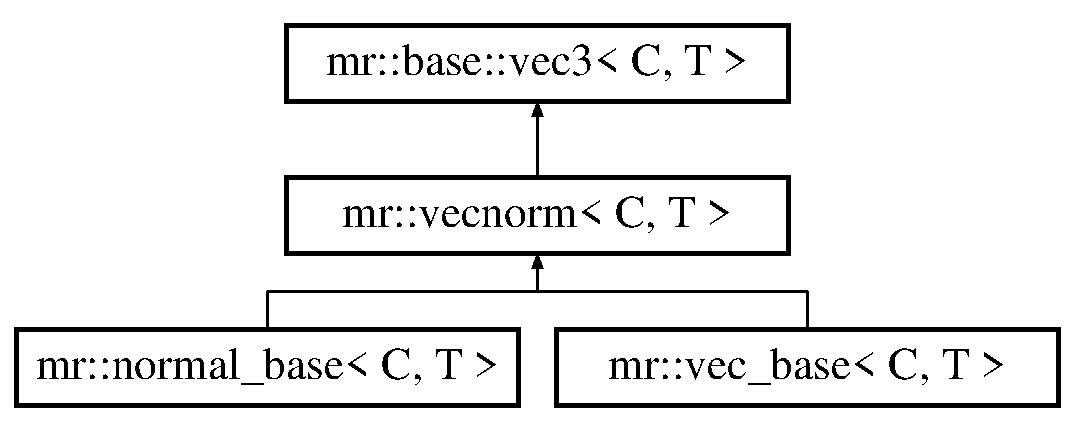
\includegraphics[height=3cm]{structmr_1_1vecnorm}
\end{center}
\end{figure}
\subsection*{Length comparisons}
\begin{CompactItemize}
\item 
bool {\bf operator$<$} (const T a) const 
\item 
bool {\bf operator$>$} (const T a) const 
\item 
bool {\bf operator$<$=} (const T a) const 
\item 
bool {\bf operator$>$=} (const T a) const 
\item 
bool {\bf operator$<$} (const {\bf vecnorm} \&a) const 
\item 
bool {\bf operator$>$} (const {\bf vecnorm} \&a) const 
\item 
bool {\bf operator$<$=} (const {\bf vecnorm} \&a) const 
\item 
bool {\bf operator$>$=} (const {\bf vecnorm} \&a) const 
\end{CompactItemize}
\subsection*{Public Types}
\begin{CompactItemize}
\item 
typedef {\bf vecnorm}$<$ C, T $>$ {\bf self}
\end{CompactItemize}
\subsection*{Public Member Functions}
\begin{CompactItemize}
\item 
{\bf vecnorm} ()
\item 
{\bf vecnorm} (const T xx, const T yy, const T zz)
\item 
T {\bf length\-Squared} () const 
\item 
T {\bf length} () const 
\item 
T {\bf inverse\-Length} () const 
\item 
T {\bf inverse\-Length\-Fast} () const 
\end{CompactItemize}
\begin{Indent}{\bf Dot product}\par
\begin{CompactItemize}
\item 
template$<$class X, class Y, class Oper$>$ T {\bf operator\%} (const {\bf base::exp}$<$ X, Y, Oper $>$ \&e) const 
\item 
T {\bf operator\%} (const mi\-Vector \&b) const 
\item 
template$<$typename X$>$ T {\bf dot} (const X \&b)
\end{CompactItemize}
\end{Indent}
\begin{Indent}{\bf Inplace operations}\par
\begin{CompactItemize}
\item 
void {\bf invert} ()
\item 
void {\bf normalize} ()
\item 
void {\bf normalize\-Fast} ()
\item 
bool {\bf is\-Normalized} () const 
\begin{CompactList}\small\item\em Return whether vector is normalized or not. \item\end{CompactList}\end{CompactItemize}
\end{Indent}
\subsubsection*{template$<$class C, typename T$>$ struct mr::vecnorm$<$ C, T $>$}



\subsection{Member Typedef Documentation}
\index{mr::vecnorm@{mr::vecnorm}!self@{self}}
\index{self@{self}!mr::vecnorm@{mr::vecnorm}}
\subsubsection{\setlength{\rightskip}{0pt plus 5cm}template$<$class C, typename T$>$ typedef {\bf vecnorm}$<$ C, T $>$ {\bf mr::vecnorm}$<$ C, T $>$::{\bf self}}\label{structmr_1_1vecnorm_w0}




Reimplemented from {\bf mr::base::vec3$<$ C, T $>$} {\rm (p.\,\pageref{structmr_1_1base_1_1vec3_w0})}.

Reimplemented in {\bf mr::vec\_\-base$<$ C, T $>$} {\rm (p.\,\pageref{structmr_1_1vec__base_w0})}, and {\bf mr::normal\_\-base$<$ C, T $>$} {\rm (p.\,\pageref{structmr_1_1normal__base_w0})}.

\subsection{Constructor \& Destructor Documentation}
\index{mr::vecnorm@{mr::vecnorm}!vecnorm@{vecnorm}}
\index{vecnorm@{vecnorm}!mr::vecnorm@{mr::vecnorm}}
\subsubsection{\setlength{\rightskip}{0pt plus 5cm}template$<$class C, typename T$>$ {\bf mr::vecnorm}$<$ C, T $>$::{\bf vecnorm} ()\hspace{0.3cm}{\tt  [inline]}}\label{structmr_1_1vecnorm_a0}


\index{mr::vecnorm@{mr::vecnorm}!vecnorm@{vecnorm}}
\index{vecnorm@{vecnorm}!mr::vecnorm@{mr::vecnorm}}
\subsubsection{\setlength{\rightskip}{0pt plus 5cm}template$<$class C, typename T$>$ {\bf mr::vecnorm}$<$ C, T $>$::{\bf vecnorm} (const T {\em xx}, const T {\em yy}, const T {\em zz})\hspace{0.3cm}{\tt  [inline]}}\label{structmr_1_1vecnorm_a1}




\subsection{Member Function Documentation}
\index{mr::vecnorm@{mr::vecnorm}!dot@{dot}}
\index{dot@{dot}!mr::vecnorm@{mr::vecnorm}}
\subsubsection{\setlength{\rightskip}{0pt plus 5cm}template$<$class C, typename T$>$ template$<$typename X$>$ T {\bf mr::vecnorm}$<$ C, T $>$::dot (const X \& {\em b})\hspace{0.3cm}{\tt  [inline]}}\label{structmr_1_1vecnorm_z55_2}


\index{mr::vecnorm@{mr::vecnorm}!inverseLength@{inverseLength}}
\index{inverseLength@{inverseLength}!mr::vecnorm@{mr::vecnorm}}
\subsubsection{\setlength{\rightskip}{0pt plus 5cm}template$<$class C, typename T$>$ T {\bf mr::vecnorm}$<$ C, T $>$::inverse\-Length () const\hspace{0.3cm}{\tt  [inline]}}\label{structmr_1_1vecnorm_a4}


\index{mr::vecnorm@{mr::vecnorm}!inverseLengthFast@{inverseLengthFast}}
\index{inverseLengthFast@{inverseLengthFast}!mr::vecnorm@{mr::vecnorm}}
\subsubsection{\setlength{\rightskip}{0pt plus 5cm}template$<$class C, typename T$>$ T {\bf mr::vecnorm}$<$ C, T $>$::inverse\-Length\-Fast () const\hspace{0.3cm}{\tt  [inline]}}\label{structmr_1_1vecnorm_a5}


\index{mr::vecnorm@{mr::vecnorm}!invert@{invert}}
\index{invert@{invert}!mr::vecnorm@{mr::vecnorm}}
\subsubsection{\setlength{\rightskip}{0pt plus 5cm}template$<$class C, typename T$>$ void {\bf mr::vecnorm}$<$ C, T $>$::invert ()\hspace{0.3cm}{\tt  [inline]}}\label{structmr_1_1vecnorm_z56_0}


\index{mr::vecnorm@{mr::vecnorm}!isNormalized@{isNormalized}}
\index{isNormalized@{isNormalized}!mr::vecnorm@{mr::vecnorm}}
\subsubsection{\setlength{\rightskip}{0pt plus 5cm}template$<$class C, typename T$>$ bool {\bf mr::vecnorm}$<$ C, T $>$::is\-Normalized () const}\label{structmr_1_1vecnorm_z56_3}


Return whether vector is normalized or not. 

\index{mr::vecnorm@{mr::vecnorm}!length@{length}}
\index{length@{length}!mr::vecnorm@{mr::vecnorm}}
\subsubsection{\setlength{\rightskip}{0pt plus 5cm}template$<$class C, typename T$>$ T {\bf mr::vecnorm}$<$ C, T $>$::length () const\hspace{0.3cm}{\tt  [inline]}}\label{structmr_1_1vecnorm_a3}


\index{mr::vecnorm@{mr::vecnorm}!lengthSquared@{lengthSquared}}
\index{lengthSquared@{lengthSquared}!mr::vecnorm@{mr::vecnorm}}
\subsubsection{\setlength{\rightskip}{0pt plus 5cm}template$<$class C, typename T$>$ T {\bf mr::vecnorm}$<$ C, T $>$::length\-Squared () const\hspace{0.3cm}{\tt  [inline]}}\label{structmr_1_1vecnorm_a2}


\index{mr::vecnorm@{mr::vecnorm}!normalize@{normalize}}
\index{normalize@{normalize}!mr::vecnorm@{mr::vecnorm}}
\subsubsection{\setlength{\rightskip}{0pt plus 5cm}template$<$class C, typename T$>$ void {\bf mr::vecnorm}$<$ C, T $>$::normalize ()\hspace{0.3cm}{\tt  [inline]}}\label{structmr_1_1vecnorm_z56_1}


\index{mr::vecnorm@{mr::vecnorm}!normalizeFast@{normalizeFast}}
\index{normalizeFast@{normalizeFast}!mr::vecnorm@{mr::vecnorm}}
\subsubsection{\setlength{\rightskip}{0pt plus 5cm}template$<$class C, typename T$>$ void {\bf mr::vecnorm}$<$ C, T $>$::normalize\-Fast ()\hspace{0.3cm}{\tt  [inline]}}\label{structmr_1_1vecnorm_z56_2}


\index{mr::vecnorm@{mr::vecnorm}!operator\%@{operator\%}}
\index{operator\%@{operator\%}!mr::vecnorm@{mr::vecnorm}}
\subsubsection{\setlength{\rightskip}{0pt plus 5cm}template$<$class C, typename T$>$ T {\bf mr::vecnorm}$<$ C, T $>$::operator\% (const mi\-Vector \& {\em b}) const\hspace{0.3cm}{\tt  [inline]}}\label{structmr_1_1vecnorm_z55_1}


\index{mr::vecnorm@{mr::vecnorm}!operator\%@{operator\%}}
\index{operator\%@{operator\%}!mr::vecnorm@{mr::vecnorm}}
\subsubsection{\setlength{\rightskip}{0pt plus 5cm}template$<$class C, typename T$>$ template$<$class X, class Y, class Oper$>$ T {\bf mr::vecnorm}$<$ C, T $>$::operator\% (const {\bf base::exp}$<$ X, Y, Oper $>$ \& {\em e}) const\hspace{0.3cm}{\tt  [inline]}}\label{structmr_1_1vecnorm_z55_0}


\index{mr::vecnorm@{mr::vecnorm}!operator<@{operator$<$}}
\index{operator<@{operator$<$}!mr::vecnorm@{mr::vecnorm}}
\subsubsection{\setlength{\rightskip}{0pt plus 5cm}template$<$class C, typename T$>$ bool {\bf mr::vecnorm}$<$ C, T $>$::operator$<$ (const {\bf vecnorm}$<$ C, T $>$ \& {\em a}) const\hspace{0.3cm}{\tt  [inline]}}\label{structmr_1_1vecnorm_z57_4}


\index{mr::vecnorm@{mr::vecnorm}!operator<@{operator$<$}}
\index{operator<@{operator$<$}!mr::vecnorm@{mr::vecnorm}}
\subsubsection{\setlength{\rightskip}{0pt plus 5cm}template$<$class C, typename T$>$ bool {\bf mr::vecnorm}$<$ C, T $>$::operator$<$ (const T {\em a}) const\hspace{0.3cm}{\tt  [inline]}}\label{structmr_1_1vecnorm_z57_0}


\index{mr::vecnorm@{mr::vecnorm}!operator<=@{operator$<$=}}
\index{operator<=@{operator$<$=}!mr::vecnorm@{mr::vecnorm}}
\subsubsection{\setlength{\rightskip}{0pt plus 5cm}template$<$class C, typename T$>$ bool {\bf mr::vecnorm}$<$ C, T $>$::operator$<$= (const {\bf vecnorm}$<$ C, T $>$ \& {\em a}) const\hspace{0.3cm}{\tt  [inline]}}\label{structmr_1_1vecnorm_z57_6}


\index{mr::vecnorm@{mr::vecnorm}!operator<=@{operator$<$=}}
\index{operator<=@{operator$<$=}!mr::vecnorm@{mr::vecnorm}}
\subsubsection{\setlength{\rightskip}{0pt plus 5cm}template$<$class C, typename T$>$ bool {\bf mr::vecnorm}$<$ C, T $>$::operator$<$= (const T {\em a}) const\hspace{0.3cm}{\tt  [inline]}}\label{structmr_1_1vecnorm_z57_2}


\index{mr::vecnorm@{mr::vecnorm}!operator>@{operator$>$}}
\index{operator>@{operator$>$}!mr::vecnorm@{mr::vecnorm}}
\subsubsection{\setlength{\rightskip}{0pt plus 5cm}template$<$class C, typename T$>$ bool {\bf mr::vecnorm}$<$ C, T $>$::operator$>$ (const {\bf vecnorm}$<$ C, T $>$ \& {\em a}) const\hspace{0.3cm}{\tt  [inline]}}\label{structmr_1_1vecnorm_z57_5}


\index{mr::vecnorm@{mr::vecnorm}!operator>@{operator$>$}}
\index{operator>@{operator$>$}!mr::vecnorm@{mr::vecnorm}}
\subsubsection{\setlength{\rightskip}{0pt plus 5cm}template$<$class C, typename T$>$ bool {\bf mr::vecnorm}$<$ C, T $>$::operator$>$ (const T {\em a}) const\hspace{0.3cm}{\tt  [inline]}}\label{structmr_1_1vecnorm_z57_1}


\index{mr::vecnorm@{mr::vecnorm}!operator>=@{operator$>$=}}
\index{operator>=@{operator$>$=}!mr::vecnorm@{mr::vecnorm}}
\subsubsection{\setlength{\rightskip}{0pt plus 5cm}template$<$class C, typename T$>$ bool {\bf mr::vecnorm}$<$ C, T $>$::operator$>$= (const {\bf vecnorm}$<$ C, T $>$ \& {\em a}) const\hspace{0.3cm}{\tt  [inline]}}\label{structmr_1_1vecnorm_z57_7}


\index{mr::vecnorm@{mr::vecnorm}!operator>=@{operator$>$=}}
\index{operator>=@{operator$>$=}!mr::vecnorm@{mr::vecnorm}}
\subsubsection{\setlength{\rightskip}{0pt plus 5cm}template$<$class C, typename T$>$ bool {\bf mr::vecnorm}$<$ C, T $>$::operator$>$= (const T {\em a}) const\hspace{0.3cm}{\tt  [inline]}}\label{structmr_1_1vecnorm_z57_3}




The documentation for this struct was generated from the following file:\begin{CompactItemize}
\item 
{\bf mr\-Vector.h}\end{CompactItemize}

\section{mr::VPerlin Class Reference}
\label{classmr_1_1VPerlin}\index{mr::VPerlin@{mr::VPerlin}}
Perlin Class returning a vector.  


{\tt \#include $<$mr\-Perlin.h$>$}

\subsection*{Static Public Member Functions}
\begin{CompactItemize}
\item 
{\bf vector} {\bf snoise} (mi\-Scalar x)
\item 
{\bf vector} {\bf snoise} (mi\-Scalar x, mi\-Scalar y)
\item 
{\bf vector} {\bf snoise} (mi\-Scalar x, mi\-Scalar y, mi\-Scalar z)
\item 
{\bf vector} {\bf snoise} (mi\-Scalar x, mi\-Scalar y, mi\-Scalar z, mi\-Scalar t)
\item 
{\bf vector} {\bf snoise} (const {\bf vector2d} \&P)
\item 
{\bf vector} {\bf snoise} (const {\bf point} \&P)
\item 
{\bf vector} {\bf snoise} (const {\bf point} \&P, const mi\-Scalar t)
\item 
{\bf vector} {\bf noise} (mi\-Scalar x)
\item 
{\bf vector} {\bf noise} (mi\-Scalar x, mi\-Scalar y)
\item 
{\bf vector} {\bf noise} (mi\-Scalar x, mi\-Scalar y, mi\-Scalar z)
\item 
{\bf vector} {\bf noise} (mi\-Scalar x, mi\-Scalar y, mi\-Scalar z, mi\-Scalar t)
\item 
{\bf vector} {\bf noise} (const {\bf vector2d} \&P)
\item 
{\bf vector} {\bf noise} (const {\bf point} \&P)
\item 
{\bf vector} {\bf noise} (const {\bf point} \&P, const mi\-Scalar t)
\item 
{\bf vector} {\bf pnoise} (const mi\-Scalar x, const mi\-Scalar period)
\item 
{\bf vector} {\bf pnoise} (const mi\-Scalar x, const mi\-Scalar y, const mi\-Scalar w, const mi\-Scalar h)
\item 
{\bf vector} {\bf pnoise} (const mi\-Scalar x, const mi\-Scalar y, const mi\-Scalar z, const mi\-Scalar w, const mi\-Scalar h, const mi\-Scalar d)
\item 
{\bf vector} {\bf pnoise} (const mi\-Scalar x, const mi\-Scalar y, const mi\-Scalar z, const mi\-Scalar t, const mi\-Scalar w, const mi\-Scalar h, const mi\-Scalar d, const mi\-Scalar p)
\item 
{\bf vector} {\bf pnoise} (const {\bf vector2d} \&P, const {\bf vector2d} \&period)
\item 
{\bf vector} {\bf pnoise} (const {\bf point} \&P, const {\bf vector} \&period)
\item 
{\bf vector} {\bf pnoise} (const {\bf point} \&P, const mi\-Scalar t, const {\bf vector} \&Pperiod, const mi\-Scalar tperiod)
\item 
{\bf vector} {\bf spnoise} (const mi\-Scalar x, const mi\-Scalar period)
\item 
{\bf vector} {\bf spnoise} (const mi\-Scalar x, const mi\-Scalar y, const mi\-Scalar w, const mi\-Scalar h)
\item 
{\bf vector} {\bf spnoise} (const mi\-Scalar x, const mi\-Scalar y, const mi\-Scalar z, const mi\-Scalar w, const mi\-Scalar h, const mi\-Scalar d)
\item 
{\bf vector} {\bf spnoise} (const mi\-Scalar x, const mi\-Scalar y, const mi\-Scalar z, const mi\-Scalar t, const mi\-Scalar w, const mi\-Scalar h, const mi\-Scalar d, const mi\-Scalar p)
\item 
{\bf vector} {\bf spnoise} (const {\bf vector2d} \&P, const {\bf vector2d} \&period)
\item 
{\bf vector} {\bf spnoise} (const {\bf point} \&P, const {\bf vector} \&period)
\item 
{\bf vector} {\bf spnoise} (const {\bf point} \&P, const mi\-Scalar t, const {\bf vector} \&Pperiod, const mi\-Scalar tperiod)
\end{CompactItemize}


\subsection{Detailed Description}
Perlin Class returning a vector. 



\subsection{Member Function Documentation}
\index{mr::VPerlin@{mr::VPerlin}!noise@{noise}}
\index{noise@{noise}!mr::VPerlin@{mr::VPerlin}}
\subsubsection{\setlength{\rightskip}{0pt plus 5cm}{\bf vector} mr::VPerlin::noise (const {\bf point} \& {\em P}, const mi\-Scalar {\em t})\hspace{0.3cm}{\tt  [inline, static]}}\label{classmr_1_1VPerlin_e13}


\index{mr::VPerlin@{mr::VPerlin}!noise@{noise}}
\index{noise@{noise}!mr::VPerlin@{mr::VPerlin}}
\subsubsection{\setlength{\rightskip}{0pt plus 5cm}{\bf vector} mr::VPerlin::noise (const {\bf point} \& {\em P})\hspace{0.3cm}{\tt  [inline, static]}}\label{classmr_1_1VPerlin_e12}


\index{mr::VPerlin@{mr::VPerlin}!noise@{noise}}
\index{noise@{noise}!mr::VPerlin@{mr::VPerlin}}
\subsubsection{\setlength{\rightskip}{0pt plus 5cm}{\bf vector} mr::VPerlin::noise (const {\bf vector2d} \& {\em P})\hspace{0.3cm}{\tt  [inline, static]}}\label{classmr_1_1VPerlin_e11}


\index{mr::VPerlin@{mr::VPerlin}!noise@{noise}}
\index{noise@{noise}!mr::VPerlin@{mr::VPerlin}}
\subsubsection{\setlength{\rightskip}{0pt plus 5cm}{\bf vector} mr::VPerlin::noise (mi\-Scalar {\em x}, mi\-Scalar {\em y}, mi\-Scalar {\em z}, mi\-Scalar {\em t})\hspace{0.3cm}{\tt  [inline, static]}}\label{classmr_1_1VPerlin_e10}


\index{mr::VPerlin@{mr::VPerlin}!noise@{noise}}
\index{noise@{noise}!mr::VPerlin@{mr::VPerlin}}
\subsubsection{\setlength{\rightskip}{0pt plus 5cm}{\bf vector} mr::VPerlin::noise (mi\-Scalar {\em x}, mi\-Scalar {\em y}, mi\-Scalar {\em z})\hspace{0.3cm}{\tt  [inline, static]}}\label{classmr_1_1VPerlin_e9}


\index{mr::VPerlin@{mr::VPerlin}!noise@{noise}}
\index{noise@{noise}!mr::VPerlin@{mr::VPerlin}}
\subsubsection{\setlength{\rightskip}{0pt plus 5cm}{\bf vector} mr::VPerlin::noise (mi\-Scalar {\em x}, mi\-Scalar {\em y})\hspace{0.3cm}{\tt  [inline, static]}}\label{classmr_1_1VPerlin_e8}


\index{mr::VPerlin@{mr::VPerlin}!noise@{noise}}
\index{noise@{noise}!mr::VPerlin@{mr::VPerlin}}
\subsubsection{\setlength{\rightskip}{0pt plus 5cm}{\bf vector} mr::VPerlin::noise (mi\-Scalar {\em x})\hspace{0.3cm}{\tt  [inline, static]}}\label{classmr_1_1VPerlin_e7}


\index{mr::VPerlin@{mr::VPerlin}!pnoise@{pnoise}}
\index{pnoise@{pnoise}!mr::VPerlin@{mr::VPerlin}}
\subsubsection{\setlength{\rightskip}{0pt plus 5cm}{\bf vector} mr::VPerlin::pnoise (const {\bf point} \& {\em P}, const mi\-Scalar {\em t}, const {\bf vector} \& {\em Pperiod}, const mi\-Scalar {\em tperiod})\hspace{0.3cm}{\tt  [inline, static]}}\label{classmr_1_1VPerlin_e20}


\index{mr::VPerlin@{mr::VPerlin}!pnoise@{pnoise}}
\index{pnoise@{pnoise}!mr::VPerlin@{mr::VPerlin}}
\subsubsection{\setlength{\rightskip}{0pt plus 5cm}{\bf vector} mr::VPerlin::pnoise (const {\bf point} \& {\em P}, const {\bf vector} \& {\em period})\hspace{0.3cm}{\tt  [inline, static]}}\label{classmr_1_1VPerlin_e19}


\index{mr::VPerlin@{mr::VPerlin}!pnoise@{pnoise}}
\index{pnoise@{pnoise}!mr::VPerlin@{mr::VPerlin}}
\subsubsection{\setlength{\rightskip}{0pt plus 5cm}{\bf vector} mr::VPerlin::pnoise (const {\bf vector2d} \& {\em P}, const {\bf vector2d} \& {\em period})\hspace{0.3cm}{\tt  [inline, static]}}\label{classmr_1_1VPerlin_e18}


\index{mr::VPerlin@{mr::VPerlin}!pnoise@{pnoise}}
\index{pnoise@{pnoise}!mr::VPerlin@{mr::VPerlin}}
\subsubsection{\setlength{\rightskip}{0pt plus 5cm}{\bf vector} mr::VPerlin::pnoise (const mi\-Scalar {\em x}, const mi\-Scalar {\em y}, const mi\-Scalar {\em z}, const mi\-Scalar {\em t}, const mi\-Scalar {\em w}, const mi\-Scalar {\em h}, const mi\-Scalar {\em d}, const mi\-Scalar {\em p})\hspace{0.3cm}{\tt  [inline, static]}}\label{classmr_1_1VPerlin_e17}


\index{mr::VPerlin@{mr::VPerlin}!pnoise@{pnoise}}
\index{pnoise@{pnoise}!mr::VPerlin@{mr::VPerlin}}
\subsubsection{\setlength{\rightskip}{0pt plus 5cm}{\bf vector} mr::VPerlin::pnoise (const mi\-Scalar {\em x}, const mi\-Scalar {\em y}, const mi\-Scalar {\em z}, const mi\-Scalar {\em w}, const mi\-Scalar {\em h}, const mi\-Scalar {\em d})\hspace{0.3cm}{\tt  [inline, static]}}\label{classmr_1_1VPerlin_e16}


\index{mr::VPerlin@{mr::VPerlin}!pnoise@{pnoise}}
\index{pnoise@{pnoise}!mr::VPerlin@{mr::VPerlin}}
\subsubsection{\setlength{\rightskip}{0pt plus 5cm}{\bf vector} mr::VPerlin::pnoise (const mi\-Scalar {\em x}, const mi\-Scalar {\em y}, const mi\-Scalar {\em w}, const mi\-Scalar {\em h})\hspace{0.3cm}{\tt  [inline, static]}}\label{classmr_1_1VPerlin_e15}


\index{mr::VPerlin@{mr::VPerlin}!pnoise@{pnoise}}
\index{pnoise@{pnoise}!mr::VPerlin@{mr::VPerlin}}
\subsubsection{\setlength{\rightskip}{0pt plus 5cm}{\bf vector} mr::VPerlin::pnoise (const mi\-Scalar {\em x}, const mi\-Scalar {\em period})\hspace{0.3cm}{\tt  [inline, static]}}\label{classmr_1_1VPerlin_e14}


\index{mr::VPerlin@{mr::VPerlin}!snoise@{snoise}}
\index{snoise@{snoise}!mr::VPerlin@{mr::VPerlin}}
\subsubsection{\setlength{\rightskip}{0pt plus 5cm}{\bf vector} mr::VPerlin::snoise (const {\bf point} \& {\em P}, const mi\-Scalar {\em t})\hspace{0.3cm}{\tt  [inline, static]}}\label{classmr_1_1VPerlin_e6}


\index{mr::VPerlin@{mr::VPerlin}!snoise@{snoise}}
\index{snoise@{snoise}!mr::VPerlin@{mr::VPerlin}}
\subsubsection{\setlength{\rightskip}{0pt plus 5cm}{\bf vector} mr::VPerlin::snoise (const {\bf point} \& {\em P})\hspace{0.3cm}{\tt  [inline, static]}}\label{classmr_1_1VPerlin_e5}


\index{mr::VPerlin@{mr::VPerlin}!snoise@{snoise}}
\index{snoise@{snoise}!mr::VPerlin@{mr::VPerlin}}
\subsubsection{\setlength{\rightskip}{0pt plus 5cm}{\bf vector} mr::VPerlin::snoise (const {\bf vector2d} \& {\em P})\hspace{0.3cm}{\tt  [inline, static]}}\label{classmr_1_1VPerlin_e4}


\index{mr::VPerlin@{mr::VPerlin}!snoise@{snoise}}
\index{snoise@{snoise}!mr::VPerlin@{mr::VPerlin}}
\subsubsection{\setlength{\rightskip}{0pt plus 5cm}{\bf vector} mr::VPerlin::snoise (mi\-Scalar {\em x}, mi\-Scalar {\em y}, mi\-Scalar {\em z}, mi\-Scalar {\em t})\hspace{0.3cm}{\tt  [inline, static]}}\label{classmr_1_1VPerlin_e3}


\index{mr::VPerlin@{mr::VPerlin}!snoise@{snoise}}
\index{snoise@{snoise}!mr::VPerlin@{mr::VPerlin}}
\subsubsection{\setlength{\rightskip}{0pt plus 5cm}{\bf vector} mr::VPerlin::snoise (mi\-Scalar {\em x}, mi\-Scalar {\em y}, mi\-Scalar {\em z})\hspace{0.3cm}{\tt  [inline, static]}}\label{classmr_1_1VPerlin_e2}


\index{mr::VPerlin@{mr::VPerlin}!snoise@{snoise}}
\index{snoise@{snoise}!mr::VPerlin@{mr::VPerlin}}
\subsubsection{\setlength{\rightskip}{0pt plus 5cm}{\bf vector} mr::VPerlin::snoise (mi\-Scalar {\em x}, mi\-Scalar {\em y})\hspace{0.3cm}{\tt  [inline, static]}}\label{classmr_1_1VPerlin_e1}


\index{mr::VPerlin@{mr::VPerlin}!snoise@{snoise}}
\index{snoise@{snoise}!mr::VPerlin@{mr::VPerlin}}
\subsubsection{\setlength{\rightskip}{0pt plus 5cm}{\bf vector} mr::VPerlin::snoise (mi\-Scalar {\em x})\hspace{0.3cm}{\tt  [inline, static]}}\label{classmr_1_1VPerlin_e0}


\index{mr::VPerlin@{mr::VPerlin}!spnoise@{spnoise}}
\index{spnoise@{spnoise}!mr::VPerlin@{mr::VPerlin}}
\subsubsection{\setlength{\rightskip}{0pt plus 5cm}{\bf vector} mr::VPerlin::spnoise (const {\bf point} \& {\em P}, const mi\-Scalar {\em t}, const {\bf vector} \& {\em Pperiod}, const mi\-Scalar {\em tperiod})\hspace{0.3cm}{\tt  [inline, static]}}\label{classmr_1_1VPerlin_e27}


\index{mr::VPerlin@{mr::VPerlin}!spnoise@{spnoise}}
\index{spnoise@{spnoise}!mr::VPerlin@{mr::VPerlin}}
\subsubsection{\setlength{\rightskip}{0pt plus 5cm}{\bf vector} mr::VPerlin::spnoise (const {\bf point} \& {\em P}, const {\bf vector} \& {\em period})\hspace{0.3cm}{\tt  [inline, static]}}\label{classmr_1_1VPerlin_e26}


\index{mr::VPerlin@{mr::VPerlin}!spnoise@{spnoise}}
\index{spnoise@{spnoise}!mr::VPerlin@{mr::VPerlin}}
\subsubsection{\setlength{\rightskip}{0pt plus 5cm}{\bf vector} mr::VPerlin::spnoise (const {\bf vector2d} \& {\em P}, const {\bf vector2d} \& {\em period})\hspace{0.3cm}{\tt  [inline, static]}}\label{classmr_1_1VPerlin_e25}


\index{mr::VPerlin@{mr::VPerlin}!spnoise@{spnoise}}
\index{spnoise@{spnoise}!mr::VPerlin@{mr::VPerlin}}
\subsubsection{\setlength{\rightskip}{0pt plus 5cm}{\bf vector} mr::VPerlin::spnoise (const mi\-Scalar {\em x}, const mi\-Scalar {\em y}, const mi\-Scalar {\em z}, const mi\-Scalar {\em t}, const mi\-Scalar {\em w}, const mi\-Scalar {\em h}, const mi\-Scalar {\em d}, const mi\-Scalar {\em p})\hspace{0.3cm}{\tt  [inline, static]}}\label{classmr_1_1VPerlin_e24}


\index{mr::VPerlin@{mr::VPerlin}!spnoise@{spnoise}}
\index{spnoise@{spnoise}!mr::VPerlin@{mr::VPerlin}}
\subsubsection{\setlength{\rightskip}{0pt plus 5cm}{\bf vector} mr::VPerlin::spnoise (const mi\-Scalar {\em x}, const mi\-Scalar {\em y}, const mi\-Scalar {\em z}, const mi\-Scalar {\em w}, const mi\-Scalar {\em h}, const mi\-Scalar {\em d})\hspace{0.3cm}{\tt  [inline, static]}}\label{classmr_1_1VPerlin_e23}


\index{mr::VPerlin@{mr::VPerlin}!spnoise@{spnoise}}
\index{spnoise@{spnoise}!mr::VPerlin@{mr::VPerlin}}
\subsubsection{\setlength{\rightskip}{0pt plus 5cm}{\bf vector} mr::VPerlin::spnoise (const mi\-Scalar {\em x}, const mi\-Scalar {\em y}, const mi\-Scalar {\em w}, const mi\-Scalar {\em h})\hspace{0.3cm}{\tt  [inline, static]}}\label{classmr_1_1VPerlin_e22}


\index{mr::VPerlin@{mr::VPerlin}!spnoise@{spnoise}}
\index{spnoise@{spnoise}!mr::VPerlin@{mr::VPerlin}}
\subsubsection{\setlength{\rightskip}{0pt plus 5cm}{\bf vector} mr::VPerlin::spnoise (const mi\-Scalar {\em x}, const mi\-Scalar {\em period})\hspace{0.3cm}{\tt  [inline, static]}}\label{classmr_1_1VPerlin_e21}




The documentation for this class was generated from the following file:\begin{CompactItemize}
\item 
{\bf mr\-Perlin.h}\end{CompactItemize}

\section{mr::warningbuffer Struct Reference}
\label{structmr_1_1warningbuffer}\index{mr::warningbuffer@{mr::warningbuffer}}
{\tt \#include $<$mr\-Stream.h$>$}

Inheritance diagram for mr::warningbuffer::\begin{figure}[H]
\begin{center}
\leavevmode
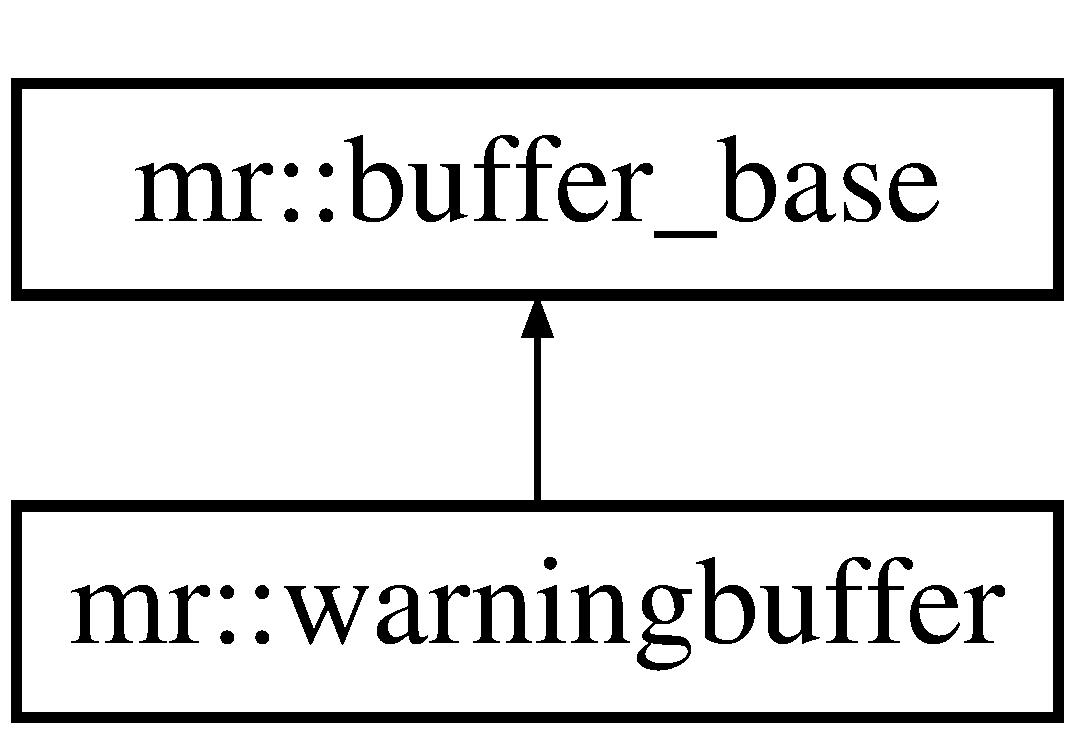
\includegraphics[height=2cm]{structmr_1_1warningbuffer}
\end{center}
\end{figure}
\subsection*{Public Member Functions}
\begin{CompactItemize}
\item 
{\bf warningbuffer} ()
\item 
virtual void {\bf print} (const char $\ast$const s)
\begin{CompactList}\small\item\em virtual function to print string out \item\end{CompactList}\end{CompactItemize}


\subsection{Constructor \& Destructor Documentation}
\index{mr::warningbuffer@{mr::warningbuffer}!warningbuffer@{warningbuffer}}
\index{warningbuffer@{warningbuffer}!mr::warningbuffer@{mr::warningbuffer}}
\subsubsection{\setlength{\rightskip}{0pt plus 5cm}mr::warningbuffer::warningbuffer ()\hspace{0.3cm}{\tt  [inline]}}\label{structmr_1_1warningbuffer_a0}




\subsection{Member Function Documentation}
\index{mr::warningbuffer@{mr::warningbuffer}!print@{print}}
\index{print@{print}!mr::warningbuffer@{mr::warningbuffer}}
\subsubsection{\setlength{\rightskip}{0pt plus 5cm}virtual void mr::warningbuffer::print (const char $\ast$const {\em s})\hspace{0.3cm}{\tt  [inline, virtual]}}\label{structmr_1_1warningbuffer_a1}


virtual function to print string out 



Implements {\bf mr::buffer\_\-base} {\rm (p.\,\pageref{structmr_1_1buffer__base_a3})}.

The documentation for this struct was generated from the following file:\begin{CompactItemize}
\item 
{\bf mr\-Stream.h}\end{CompactItemize}

\section{mr::warningstream Struct Reference}
\label{structmr_1_1warningstream}\index{mr::warningstream@{mr::warningstream}}
{\tt \#include $<$mr\-Stream.h$>$}

\subsection*{Public Member Functions}
\begin{CompactItemize}
\item 
{\bf warningstream} ()
\item 
{\bf $\sim$warningstream} ()
\end{CompactItemize}


\subsection{Constructor \& Destructor Documentation}
\index{mr::warningstream@{mr::warningstream}!warningstream@{warningstream}}
\index{warningstream@{warningstream}!mr::warningstream@{mr::warningstream}}
\subsubsection{\setlength{\rightskip}{0pt plus 5cm}mr::warningstream::warningstream ()\hspace{0.3cm}{\tt  [inline]}}\label{structmr_1_1warningstream_a0}


\index{mr::warningstream@{mr::warningstream}!~warningstream@{$\sim$warningstream}}
\index{~warningstream@{$\sim$warningstream}!mr::warningstream@{mr::warningstream}}
\subsubsection{\setlength{\rightskip}{0pt plus 5cm}mr::warningstream::$\sim${\bf warningstream} ()\hspace{0.3cm}{\tt  [inline]}}\label{structmr_1_1warningstream_a1}




The documentation for this struct was generated from the following file:\begin{CompactItemize}
\item 
{\bf mr\-Stream.h}\end{CompactItemize}

\chapter{mr\-Classes File Documentation}
\section{mr\-Assert.h File Reference}
\label{mrAssert_8h}\index{mrAssert.h@{mrAssert.h}}
{\tt \#include \char`\"{}mr\-Platform.h\char`\"{}}\par
\subsection*{Defines}
\begin{CompactItemize}
\item 
\#define {\bf mr\-ASSERT}(x)
\item 
\#define {\bf mr\-FAIL}(x)
\end{CompactItemize}


\subsection{Define Documentation}
\index{mrAssert.h@{mr\-Assert.h}!mrASSERT@{mrASSERT}}
\index{mrASSERT@{mrASSERT}!mrAssert.h@{mr\-Assert.h}}
\subsubsection{\setlength{\rightskip}{0pt plus 5cm}\#define mr\-ASSERT(x)}\label{mrAssert_8h_a0}


Just a simple include that adds ASSERTIONS for compile-time debugging \index{mrAssert.h@{mr\-Assert.h}!mrFAIL@{mrFAIL}}
\index{mrFAIL@{mrFAIL}!mrAssert.h@{mr\-Assert.h}}
\subsubsection{\setlength{\rightskip}{0pt plus 5cm}\#define mr\-FAIL(x)}\label{mrAssert_8h_a1}


{\bf Value:}

\footnotesize\begin{verbatim}do { \
                         mi_error( "FAIL! at %s, %s, line %d.", \
                                  __FILE__, __FUNCTION__, __LINE__ ); \
                         mr_error(x); \
                         mi_fatal( "Aborting render..." ); \
                    } while(0);
\end{verbatim}\normalsize 

\section{mr\-Aux.h File Reference}
\label{mrAux_8h}\index{mrAux.h@{mrAux.h}}
{\tt \#include \char`\"{}mr\-Platform.h\char`\"{}}\par
{\tt \#include \char`\"{}mr\-Macros.h\char`\"{}}\par
{\tt \#include \char`\"{}mr\-Assert.h\char`\"{}}\par
{\tt \#include \char`\"{}mr\-Memory.h\char`\"{}}\par
{\tt \#include \char`\"{}mr\-Stream.h\char`\"{}}\par
{\tt \#include \char`\"{}mr\-Functors.h\char`\"{}}\par
\subsection*{Namespaces}
\begin{CompactItemize}
\item 
namespace {\bf mr}
\end{CompactItemize}

\section{mr\-Base.h File Reference}
\label{mrBase_8h}\index{mrBase.h@{mrBase.h}}
{\tt \#include \char`\"{}shader.h\char`\"{}}\par
{\tt \#include \char`\"{}mr\-Macros.h\char`\"{}}\par
\subsection*{Namespaces}
\begin{CompactItemize}
\item 
namespace {\bf mr}
\item 
namespace {\bf mr::base}
\end{CompactItemize}

\section{mr\-Bump.h File Reference}
\label{mrBump_8h}\index{mrBump.h@{mrBump.h}}
{\tt \#include \char`\"{}mr\-Macros.h\char`\"{}}\par
{\tt \#include \char`\"{}mr\-Vector.h\char`\"{}}\par
{\tt \#include \char`\"{}mr\-Operators.h\char`\"{}}\par
\subsection*{Namespaces}
\begin{CompactItemize}
\item 
namespace {\bf mr}
\end{CompactItemize}

\section{mr\-Cache.h File Reference}
\label{mrCache_8h}\index{mrCache.h@{mrCache.h}}
{\tt \#include $<$map$>$}\par
{\tt \#include $<$algorithm$>$}\par
{\tt \#include \char`\"{}mr\-Memory.h\char`\"{}}\par
{\tt \#include \char`\"{}mr\-Sampler.h\char`\"{}}\par
{\tt \#include \char`\"{}mr\-Color.h\char`\"{}}\par
{\tt \#include \char`\"{}mr\-Derivs.h\char`\"{}}\par
\subsection*{Namespaces}
\begin{CompactItemize}
\item 
namespace {\bf mr}
\end{CompactItemize}

\section{mr\-Cell.h File Reference}
\label{mrCell_8h}\index{mrCell.h@{mrCell.h}}
{\tt \#include \char`\"{}mr\-Vector.h\char`\"{}}\par
\subsection*{Namespaces}
\begin{CompactItemize}
\item 
namespace {\bf mr}
\end{CompactItemize}
\subsection*{Defines}
\begin{CompactItemize}
\item 
\#define {\bf mr\-EPS}\ mi\-SCALAR\_\-EPSILON
\end{CompactItemize}


\subsection{Define Documentation}
\index{mrCell.h@{mr\-Cell.h}!mrEPS@{mrEPS}}
\index{mrEPS@{mrEPS}!mrCell.h@{mr\-Cell.h}}
\subsubsection{\setlength{\rightskip}{0pt plus 5cm}\#define mr\-EPS\ mi\-SCALAR\_\-EPSILON}\label{mrCell_8h_a0}



\section{mr\-Color.h File Reference}
\label{mrColor_8h}\index{mrColor.h@{mrColor.h}}
{\tt \#include \char`\"{}mr\-Operators.h\char`\"{}}\par
{\tt \#include \char`\"{}mr\-Swizzle.h\char`\"{}}\par
{\tt \#include \char`\"{}mr\-Un\-Swizzle.h\char`\"{}}\par
{\tt \#include \char`\"{}mr\-Color.inl\char`\"{}}\par
{\tt \#include \char`\"{}mr\-Stream.h\char`\"{}}\par
{\tt \#include \char`\"{}mr\-Vector.h\char`\"{}}\par
\subsection*{Namespaces}
\begin{CompactItemize}
\item 
namespace {\bf mr}
\end{CompactItemize}

\section{mr\-Derivs.h File Reference}
\label{mrDerivs_8h}\index{mrDerivs.h@{mrDerivs.h}}
{\tt \#include $<$set$>$}\par
{\tt \#include \char`\"{}mr\-Vector.h\char`\"{}}\par
\subsection*{Namespaces}
\begin{CompactItemize}
\item 
namespace {\bf mr}
\end{CompactItemize}

\section{mr\-Distances.h File Reference}
\label{mrDistances_8h}\index{mrDistances.h@{mrDistances.h}}
{\tt \#include \char`\"{}mr\-Vector.h\char`\"{}}\par
\subsection*{Namespaces}
\begin{CompactItemize}
\item 
namespace {\bf mr}
\item 
namespace {\bf mr::distances}
\end{CompactItemize}

\section{mr\-Fast\-Math.h File Reference}
\label{mrFastMath_8h}\index{mrFastMath.h@{mrFastMath.h}}
{\tt \#include \char`\"{}mr\-Macros.h\char`\"{}}\par
{\tt \#include \char`\"{}mr\-Memory.h\char`\"{}}\par
\subsection*{Namespaces}
\begin{CompactItemize}
\item 
namespace {\bf mr}
\end{CompactItemize}

\section{mr\-Filters.h File Reference}
\label{mrFilters_8h}\index{mrFilters.h@{mrFilters.h}}
{\tt \#include \char`\"{}mr\-Macros.h\char`\"{}}\par
{\tt \#include \char`\"{}mr\-Math.h\char`\"{}}\par
\subsection*{Namespaces}
\begin{CompactItemize}
\item 
namespace {\bf mr}
\item 
namespace {\bf mr::filter}
\end{CompactItemize}

\section{mr\-Functors.h File Reference}
\label{mrFunctors_8h}\index{mrFunctors.h@{mrFunctors.h}}
{\tt \#include \char`\"{}mr\-Memory.h\char`\"{}}\par
\subsection*{Namespaces}
\begin{CompactItemize}
\item 
namespace {\bf mr}
\end{CompactItemize}

\section{mr\-Generics.h File Reference}
\label{mrGenerics_8h}\index{mrGenerics.h@{mrGenerics.h}}
{\tt \#include \char`\"{}mr\-Operators.h\char`\"{}}\par
{\tt \#include \char`\"{}mr\-Color.h\char`\"{}}\par
{\tt \#include \char`\"{}mr\-Derivs.h\char`\"{}}\par
{\tt \#include \char`\"{}mr\-Spline.h\char`\"{}}\par
{\tt \#include \char`\"{}mr\-Sampler.h\char`\"{}}\par
{\tt \#include \char`\"{}mr\-Parameters.h\char`\"{}}\par
{\tt \#include \char`\"{}mr\-Bump.h\char`\"{}}\par
{\tt \#include \char`\"{}mr\-Perlin.h\char`\"{}}\par
{\tt \#include \char`\"{}mr\-Cell.h\char`\"{}}\par
{\tt \#include \char`\"{}mr\-Worley.h\char`\"{}}\par
{\tt \#include \char`\"{}mr\-Point\-Cache.h\char`\"{}}\par
{\tt \#include \char`\"{}mr\-Profile.h\char`\"{}}\par
{\tt \#include \char`\"{}mr\-Mem\-Check.h\char`\"{}}\par
{\tt \#include \char`\"{}mr\-Shading.h\char`\"{}}\par

\section{mr\-Interval.h File Reference}
\label{mrInterval_8h}\index{mrInterval.h@{mrInterval.h}}
\subsection*{Classes}
\begin{CompactItemize}
\item 
class {\bf interval}
\end{CompactItemize}

\section{mr\-Linux.h File Reference}
\label{mrLinux_8h}\index{mrLinux.h@{mrLinux.h}}
{\tt \#include \char`\"{}mr\-Stack\-Trace\_\-linux.h\char`\"{}}\par

\section{mr\-Macros.h File Reference}
\label{mrMacros_8h}\index{mrMacros.h@{mrMacros.h}}
\subsection*{Defines}
\begin{CompactItemize}
\item 
\#define {\bf BEGIN\_\-NAMESPACE}(NAME\_\-STRING)\ namespace NAME\_\-STRING \{
\item 
\#define {\bf END\_\-NAMESPACE}(NAME\_\-STRING)\ \}
\item 
\#define {\bf EXTERN\_\-C}\ extern \char`\"{}C\char`\"{}
\item 
\#define {\bf ISNAN}(x)\ ::isnan(x)
\end{CompactItemize}


\subsection{Define Documentation}
\index{mrMacros.h@{mr\-Macros.h}!BEGIN_NAMESPACE@{BEGIN\_\-NAMESPACE}}
\index{BEGIN_NAMESPACE@{BEGIN\_\-NAMESPACE}!mrMacros.h@{mr\-Macros.h}}
\subsubsection{\setlength{\rightskip}{0pt plus 5cm}\#define BEGIN\_\-NAMESPACE(NAME\_\-STRING)\ namespace NAME\_\-STRING \{}\label{mrMacros_8h_a0}


\index{mrMacros.h@{mr\-Macros.h}!END_NAMESPACE@{END\_\-NAMESPACE}}
\index{END_NAMESPACE@{END\_\-NAMESPACE}!mrMacros.h@{mr\-Macros.h}}
\subsubsection{\setlength{\rightskip}{0pt plus 5cm}\#define END\_\-NAMESPACE(NAME\_\-STRING)\ \}}\label{mrMacros_8h_a1}


\index{mrMacros.h@{mr\-Macros.h}!EXTERN_C@{EXTERN\_\-C}}
\index{EXTERN_C@{EXTERN\_\-C}!mrMacros.h@{mr\-Macros.h}}
\subsubsection{\setlength{\rightskip}{0pt plus 5cm}\#define EXTERN\_\-C\ extern \char`\"{}C\char`\"{}}\label{mrMacros_8h_a2}


\index{mrMacros.h@{mr\-Macros.h}!ISNAN@{ISNAN}}
\index{ISNAN@{ISNAN}!mrMacros.h@{mr\-Macros.h}}
\subsubsection{\setlength{\rightskip}{0pt plus 5cm}\#define ISNAN(x)\ ::isnan(x)}\label{mrMacros_8h_a3}



\section{mr\-Math.h File Reference}
\label{mrMath_8h}\index{mrMath.h@{mrMath.h}}
{\tt \#include $<$cmath$>$}\par
{\tt \#include \char`\"{}mr\-Fast\-Math.h\char`\"{}}\par
{\tt \#include $<$shader.h$>$}\par
{\tt \#include \char`\"{}mr\-Assert.h\char`\"{}}\par
{\tt \#include \char`\"{}mr\-Macros.h\char`\"{}}\par
\subsection*{Namespaces}
\begin{CompactItemize}
\item 
namespace {\bf mr}
\end{CompactItemize}

\section{mr\-Matrix.h File Reference}
\label{mrMatrix_8h}\index{mrMatrix.h@{mrMatrix.h}}
{\tt \#include \char`\"{}mr\-Aux.h\char`\"{}}\par
{\tt \#include \char`\"{}mr\-Math.h\char`\"{}}\par
{\tt \#include \char`\"{}mr\-Matrix.inl\char`\"{}}\par
\subsection*{Namespaces}
\begin{CompactItemize}
\item 
namespace {\bf mr}
\end{CompactItemize}

\section{mr\-Mem\-Check.h File Reference}
\label{mrMemCheck_8h}\index{mrMemCheck.h@{mrMemCheck.h}}

\section{mr\-Memory.h File Reference}
\label{mrMemory_8h}\index{mrMemory.h@{mrMemory.h}}
{\tt \#include $<$shader.h$>$}\par
{\tt \#include $<$new$>$}\par
{\tt \#include \char`\"{}mr\-Platform.h\char`\"{}}\par
{\tt \#include \char`\"{}mr\-Macros.h\char`\"{}}\par
\subsection*{Functions}
\begin{CompactItemize}
\item 
void $\ast$ {\bf operator new} (size\_\-t size)  throw (std::bad\_\-alloc)
\item 
void $\ast$ {\bf operator new[$\,$]} (size\_\-t size)  throw (std::bad\_\-alloc)
\item 
void {\bf operator delete} (void $\ast$ptr)  throw ()
\item 
void {\bf operator delete[$\,$]} (void $\ast$ptr)  throw ()
\end{CompactItemize}


\subsection{Function Documentation}
\index{mrMemory.h@{mr\-Memory.h}!operator delete@{operator delete}}
\index{operator delete@{operator delete}!mrMemory.h@{mr\-Memory.h}}
\subsubsection{\setlength{\rightskip}{0pt plus 5cm}void operator delete (void $\ast$ {\em ptr})  throw ()\hspace{0.3cm}{\tt  [inline]}}\label{mrMemory_8h_a2}


\index{mrMemory.h@{mr\-Memory.h}!operator delete[]@{operator delete[]}}
\index{operator delete[]@{operator delete[]}!mrMemory.h@{mr\-Memory.h}}
\subsubsection{\setlength{\rightskip}{0pt plus 5cm}void operator delete[$\,$] (void $\ast$ {\em ptr})  throw ()\hspace{0.3cm}{\tt  [inline]}}\label{mrMemory_8h_a3}


\index{mrMemory.h@{mr\-Memory.h}!operator new@{operator new}}
\index{operator new@{operator new}!mrMemory.h@{mr\-Memory.h}}
\subsubsection{\setlength{\rightskip}{0pt plus 5cm}void$\ast$ operator new (size\_\-t {\em size})  throw (std::bad\_\-alloc)\hspace{0.3cm}{\tt  [inline]}}\label{mrMemory_8h_a0}


Override the global new/delete operators to allow tracking of memory leaks. \index{mrMemory.h@{mr\-Memory.h}!operator new[]@{operator new[]}}
\index{operator new[]@{operator new[]}!mrMemory.h@{mr\-Memory.h}}
\subsubsection{\setlength{\rightskip}{0pt plus 5cm}void$\ast$ operator new[$\,$] (size\_\-t {\em size})  throw (std::bad\_\-alloc)\hspace{0.3cm}{\tt  [inline]}}\label{mrMemory_8h_a1}



\section{mr\-Memory\-Dbg.h File Reference}
\label{mrMemoryDbg_8h}\index{mrMemoryDbg.h@{mrMemoryDbg.h}}
{\tt \#include \char`\"{}mr\-Platform.h\char`\"{}}\par
{\tt \#include $<$new$>$}\par
{\tt \#include $<$stdio.h$>$}\par
{\tt \#include \char`\"{}shader.h\char`\"{}}\par
\subsection*{Functions}
\begin{CompactItemize}
\item 
void {\bf Start\_\-Memory\-Debug} ()
\item 
void {\bf End\_\-Memory\-Debug} ()
\item 
MR\_\-LIB\_\-EXPORT void {\bf \_\-dbg\_\-delete} (void $\ast$addr)
\item 
MR\_\-LIB\_\-EXPORT void $\ast$ {\bf \_\-dbg\_\-alloc} (size\_\-t size, const unsigned int line, const char $\ast$const file)
\end{CompactItemize}
\subsection*{Variables}
\begin{CompactItemize}
\item 
MR\_\-LIB\_\-EXPORT mi\-Lock {\bf \_\-mem\-Alloc\-Lock}
\end{CompactItemize}


\subsection{Function Documentation}
\index{mrMemoryDbg.h@{mr\-Memory\-Dbg.h}!_dbg_alloc@{\_\-dbg\_\-alloc}}
\index{_dbg_alloc@{\_\-dbg\_\-alloc}!mrMemoryDbg.h@{mr\-Memory\-Dbg.h}}
\subsubsection{\setlength{\rightskip}{0pt plus 5cm}MR\_\-LIB\_\-EXPORT void$\ast$ \_\-dbg\_\-alloc (size\_\-t {\em size}, const unsigned int {\em line}, const char $\ast$const {\em file})}\label{mrMemoryDbg_8h_a4}


\index{mrMemoryDbg.h@{mr\-Memory\-Dbg.h}!_dbg_delete@{\_\-dbg\_\-delete}}
\index{_dbg_delete@{\_\-dbg\_\-delete}!mrMemoryDbg.h@{mr\-Memory\-Dbg.h}}
\subsubsection{\setlength{\rightskip}{0pt plus 5cm}MR\_\-LIB\_\-EXPORT void \_\-dbg\_\-delete (void $\ast$ {\em addr})}\label{mrMemoryDbg_8h_a3}


\index{mrMemoryDbg.h@{mr\-Memory\-Dbg.h}!End_MemoryDebug@{End\_\-MemoryDebug}}
\index{End_MemoryDebug@{End\_\-MemoryDebug}!mrMemoryDbg.h@{mr\-Memory\-Dbg.h}}
\subsubsection{\setlength{\rightskip}{0pt plus 5cm}void End\_\-Memory\-Debug ()}\label{mrMemoryDbg_8h_a2}


\index{mrMemoryDbg.h@{mr\-Memory\-Dbg.h}!Start_MemoryDebug@{Start\_\-MemoryDebug}}
\index{Start_MemoryDebug@{Start\_\-MemoryDebug}!mrMemoryDbg.h@{mr\-Memory\-Dbg.h}}
\subsubsection{\setlength{\rightskip}{0pt plus 5cm}void Start\_\-Memory\-Debug ()}\label{mrMemoryDbg_8h_a1}




\subsection{Variable Documentation}
\index{mrMemoryDbg.h@{mr\-Memory\-Dbg.h}!_memAllocLock@{\_\-memAllocLock}}
\index{_memAllocLock@{\_\-memAllocLock}!mrMemoryDbg.h@{mr\-Memory\-Dbg.h}}
\subsubsection{\setlength{\rightskip}{0pt plus 5cm}MR\_\-LIB\_\-EXPORT mi\-Lock {\bf \_\-mem\-Alloc\-Lock}}\label{mrMemoryDbg_8h_a0}



\section{mr\-Mutex.h File Reference}
\label{mrMutex_8h}\index{mrMutex.h@{mrMutex.h}}
{\tt \#include \char`\"{}mr\-Mutex.inl\char`\"{}}\par
{\tt \#include \char`\"{}shader.h\char`\"{}}\par
{\tt \#include \char`\"{}mr\-Macros.h\char`\"{}}\par
\subsection*{Namespaces}
\begin{CompactItemize}
\item 
namespace {\bf mr}
\end{CompactItemize}

\section{mr\-Operators.h File Reference}
\label{mrOperators_8h}\index{mrOperators.h@{mrOperators.h}}
{\tt \#include \char`\"{}mr\-Assert.h\char`\"{}}\par
{\tt \#include \char`\"{}mr\-Base.h\char`\"{}}\par
\subsection*{Defines}
\begin{CompactItemize}
\item 
\#define {\bf CHECK\_\-NANS}
\end{CompactItemize}
\subsection*{Functions}
\begin{CompactItemize}
\item 
mi\-Color {\bf operator-} (const mi\-Color \&x)
\item 
mi\-Color {\bf operator+} (const mi\-Color \&a, const mi\-Color \&b)
\item 
mi\-Color {\bf operator+} (const mi\-Color \&a, const mi\-Scalar b)
\item 
template$<$class X, class Y, class Oper$>$ mi\-Color {\bf operator+} (const mi\-Color \&a, const {\bf mr::base::exp}$<$ X, Y, Oper $>$ \&b)
\item 
mi\-Color {\bf operator-} (const mi\-Color \&a, const mi\-Color \&b)
\item 
mi\-Color {\bf operator-} (const mi\-Color \&a, const mi\-Scalar b)
\item 
template$<$class X, class Y, class Oper$>$ mi\-Color {\bf operator-} (const mi\-Color \&a, const {\bf mr::base::exp}$<$ X, Y, Oper $>$ \&b)
\item 
mi\-Color {\bf operator $\ast$} (const mi\-Color \&a, const mi\-Color \&b)
\item 
mi\-Color {\bf operator $\ast$} (const mi\-Scalar b, const mi\-Color \&a)
\item 
mi\-Color {\bf operator $\ast$} (const mi\-Color \&a, const mi\-Scalar b)
\item 
template$<$class X, class Y, class Oper$>$ mi\-Color {\bf operator $\ast$} (const mi\-Color \&a, const {\bf mr::base::exp}$<$ X, Y, Oper $>$ \&b)
\item 
mi\-Color {\bf operator/} (const mi\-Color \&a, const mi\-Color \&b)
\item 
mi\-Color {\bf operator/} (const mi\-Color \&a, const mi\-Scalar \&b)
\item 
template$<$class X, class Y, class Oper$>$ mi\-Color {\bf operator/} (const mi\-Color \&a, const {\bf mr::base::exp}$<$ X, Y, Oper $>$ \&b)
\item 
const mi\-Color \& {\bf operator+=} (mi\-Color \&a, const mi\-Color \&b)
\item 
const mi\-Color \& {\bf operator+=} (mi\-Color \&a, const mi\-Scalar b)
\item 
template$<$class X, class Y, class Oper$>$ mi\-Color {\bf operator+=} (mi\-Color \&a, const {\bf mr::base::exp}$<$ X, Y, Oper $>$ \&b)
\item 
const mi\-Color \& {\bf operator-=} (mi\-Color \&a, const mi\-Color \&b)
\item 
const mi\-Color \& {\bf operator-=} (mi\-Color \&a, const mi\-Scalar b)
\item 
template$<$class X, class Y, class Oper$>$ mi\-Color {\bf operator-=} (mi\-Color \&a, const {\bf mr::base::exp}$<$ X, Y, Oper $>$ \&b)
\item 
const mi\-Color \& {\bf operator $\ast$=} (mi\-Color \&a, const mi\-Color \&b)
\item 
const mi\-Color \& {\bf operator $\ast$=} (mi\-Color \&a, const mi\-Scalar x)
\item 
template$<$class X, class Y, class Oper$>$ mi\-Color {\bf operator $\ast$=} (mi\-Color \&a, const {\bf mr::base::exp}$<$ X, Y, Oper $>$ \&b)
\item 
const mi\-Color \& {\bf operator/=} (mi\-Color \&a, const mi\-Color \&b)
\item 
template$<$class X, class Y, class Oper$>$ mi\-Color {\bf operator/=} (mi\-Color \&a, const {\bf mr::base::exp}$<$ X, Y, Oper $>$ \&b)
\item 
mi\-Vector {\bf operator-} (const mi\-Vector \&a)
\item 
const mi\-Vector \& {\bf operator+=} (mi\-Vector \&a, const mi\-Scalar b)
\item 
const mi\-Vector \& {\bf operator+=} (mi\-Vector \&a, const mi\-Vector \&b)
\item 
template$<$class X, class Y, class Oper$>$ mi\-Vector {\bf operator+=} (mi\-Vector \&a, const {\bf mr::base::exp}$<$ X, Y, Oper $>$ \&b)
\item 
const mi\-Vector \& {\bf operator-=} (mi\-Vector \&a, const mi\-Scalar b)
\item 
const mi\-Vector \& {\bf operator-=} (mi\-Vector \&a, const mi\-Vector \&b)
\item 
template$<$class X, class Y, class Oper$>$ mi\-Vector {\bf operator-=} (mi\-Vector \&a, const {\bf mr::base::exp}$<$ X, Y, Oper $>$ \&b)
\item 
const mi\-Vector \& {\bf operator $\ast$=} (mi\-Vector \&a, const mi\-Scalar b)
\item 
template$<$class X, class Y, class Oper$>$ mi\-Vector {\bf operator $\ast$=} (mi\-Vector \&a, const {\bf mr::base::exp}$<$ X, Y, Oper $>$ \&b)
\item 
const mi\-Vector \& {\bf operator $\ast$=} (mi\-Vector \&a, const mi\-Vector \&b)
\item 
const mi\-Vector \& {\bf operator/=} (mi\-Vector \&a, const mi\-Scalar b)
\item 
const mi\-Vector \& {\bf operator/=} (mi\-Vector \&a, const mi\-Vector \&b)
\item 
template$<$class X, class Y, class Oper$>$ mi\-Vector {\bf operator/=} (mi\-Vector \&a, const {\bf mr::base::exp}$<$ X, Y, Oper $>$ \&b)
\item 
mi\-Scalar {\bf operator\%} (const mi\-Vector \&a, const mi\-Vector \&b)
\item 
template$<$class X, class Y, class Oper$>$ mi\-Scalar {\bf operator\%} (const mi\-Vector \&a, const {\bf mr::base::exp}$<$ X, Y, Oper $>$ \&b)
\item 
mi\-Geo\-Vector {\bf operator-} (const mi\-Geo\-Vector \&a)
\item 
const mi\-Geo\-Vector \& {\bf operator+=} (mi\-Geo\-Vector \&a, const mi\-Geo\-Scalar b)
\item 
const mi\-Geo\-Vector \& {\bf operator+=} (mi\-Geo\-Vector \&a, const mi\-Vector \&b)
\item 
const mi\-Geo\-Vector \& {\bf operator+=} (mi\-Geo\-Vector \&a, const mi\-Geo\-Vector \&b)
\item 
template$<$class X, class Y, class Oper$>$ mi\-Geo\-Vector {\bf operator+=} (mi\-Geo\-Vector \&a, const {\bf mr::base::exp}$<$ X, Y, Oper $>$ \&b)
\item 
const mi\-Geo\-Vector \& {\bf operator-=} (mi\-Geo\-Vector \&a, const mi\-Geo\-Scalar b)
\item 
const mi\-Geo\-Vector \& {\bf operator-=} (mi\-Geo\-Vector \&a, const mi\-Vector \&b)
\item 
const mi\-Geo\-Vector \& {\bf operator-=} (mi\-Geo\-Vector \&a, const mi\-Geo\-Vector \&b)
\item 
template$<$class X, class Y, class Oper$>$ mi\-Geo\-Vector {\bf operator-=} (mi\-Geo\-Vector \&a, const {\bf mr::base::exp}$<$ X, Y, Oper $>$ \&b)
\item 
const mi\-Geo\-Vector \& {\bf operator $\ast$=} (mi\-Geo\-Vector \&a, const mi\-Geo\-Scalar b)
\item 
const mi\-Geo\-Vector \& {\bf operator $\ast$=} (mi\-Geo\-Vector \&a, const mi\-Vector \&b)
\item 
const mi\-Geo\-Vector \& {\bf operator $\ast$=} (mi\-Geo\-Vector \&a, const mi\-Geo\-Vector \&b)
\item 
template$<$class X, class Y, class Oper$>$ mi\-Geo\-Vector {\bf operator $\ast$=} (mi\-Geo\-Vector \&a, const {\bf mr::base::exp}$<$ X, Y, Oper $>$ \&b)
\item 
const mi\-Geo\-Vector \& {\bf operator/=} (mi\-Geo\-Vector \&a, const mi\-Geo\-Scalar b)
\item 
const mi\-Geo\-Vector \& {\bf operator/=} (mi\-Geo\-Vector \&a, const mi\-Vector \&b)
\item 
const mi\-Geo\-Vector \& {\bf operator/=} (mi\-Geo\-Vector \&a, const mi\-Geo\-Vector \&b)
\item 
template$<$class X, class Y, class Oper$>$ mi\-Geo\-Vector {\bf operator/=} (mi\-Geo\-Vector \&a, const {\bf mr::base::exp}$<$ X, Y, Oper $>$ \&b)
\item 
mi\-Geo\-Scalar {\bf operator\%} (const mi\-Vector \&a, const mi\-Geo\-Vector \&b)
\item 
mi\-Geo\-Scalar {\bf operator\%} (const mi\-Geo\-Vector \&a, const mi\-Vector \&b)
\item 
mi\-Geo\-Scalar {\bf operator\%} (const mi\-Geo\-Vector \&a, const mi\-Geo\-Vector \&b)
\item 
template$<$typename T$>$ mi\-Vector {\bf operator+} (const mi\-Vector \&a, const T \&b)
\item 
template$<$typename T$>$ mi\-Geo\-Vector {\bf operator+} (const mi\-Geo\-Vector \&a, const T \&b)
\item 
template$<$typename T$>$ mi\-Vector {\bf operator-} (const mi\-Vector \&a, const T \&b)
\item 
template$<$typename T$>$ mi\-Geo\-Vector {\bf operator-} (const mi\-Geo\-Vector \&a, const T \&b)
\item 
template$<$typename T$>$ mi\-Vector {\bf operator $\ast$} (const T \&b, const mi\-Vector \&a)
\item 
template$<$typename T$>$ mi\-Vector {\bf operator $\ast$} (const mi\-Vector \&a, const T \&b)
\item 
template$<$typename T$>$ mi\-Geo\-Vector {\bf operator $\ast$} (const T \&b, const mi\-Geo\-Vector \&a)
\item 
template$<$typename T$>$ mi\-Geo\-Vector {\bf operator $\ast$} (const mi\-Geo\-Vector \&a, const T \&b)
\item 
template$<$typename T$>$ mi\-Vector {\bf operator/} (const mi\-Vector \&a, const T \&b)
\item 
template$<$typename T$>$ mi\-Geo\-Vector {\bf operator/} (const mi\-Geo\-Vector \&a, const T \&b)
\item 
template$<$class X, class Y, class Oper$>$ mi\-Geo\-Scalar {\bf operator\%} (const mi\-Geo\-Vector \&a, const {\bf mr::base::exp}$<$ X, Y, Oper $>$ \&b)
\item 
template$<$class X, class Y, class Oper$>$ mi\-Vector {\bf operator$^\wedge$} (const mi\-Vector \&a, const {\bf mr::base::exp}$<$ X, Y, Oper $>$ \&b)
\item 
mi\-Vector {\bf operator$^\wedge$} (const mi\-Vector \&a, const mi\-Vector \&b)
\item 
mi\-Geo\-Vector {\bf operator$^\wedge$} (const mi\-Geo\-Vector \&a, const mi\-Geo\-Vector \&b)
\item 
mi\-Geo\-Vector {\bf operator$^\wedge$} (const mi\-Geo\-Vector \&a, const mi\-Vector \&b)
\item 
template$<$class X, class Y, class Oper$>$ mi\-Geo\-Vector {\bf operator$^\wedge$} (const mi\-Geo\-Vector \&a, const {\bf mr::base::exp}$<$ X, Y, Oper $>$ \&b)
\end{CompactItemize}


\subsection{Define Documentation}
\index{mrOperators.h@{mr\-Operators.h}!CHECK_NANS@{CHECK\_\-NANS}}
\index{CHECK_NANS@{CHECK\_\-NANS}!mrOperators.h@{mr\-Operators.h}}
\subsubsection{\setlength{\rightskip}{0pt plus 5cm}\#define CHECK\_\-NANS}\label{mrOperators_8h_a0}


Simple overloading of all common operators for standard mi..types. Note that these operators may not be as optimal as the actual mr:: classes. 

\subsection{Function Documentation}
\index{mrOperators.h@{mr\-Operators.h}!operator *@{operator $\ast$}}
\index{operator *@{operator $\ast$}!mrOperators.h@{mr\-Operators.h}}
\subsubsection{\setlength{\rightskip}{0pt plus 5cm}template$<$typename T$>$ mi\-Geo\-Vector operator $\ast$ (const mi\-Geo\-Vector \& {\em a}, const T \& {\em b})\hspace{0.3cm}{\tt  [inline]}}\label{mrOperators_8h_a68}


\index{mrOperators.h@{mr\-Operators.h}!operator *@{operator $\ast$}}
\index{operator *@{operator $\ast$}!mrOperators.h@{mr\-Operators.h}}
\subsubsection{\setlength{\rightskip}{0pt plus 5cm}template$<$typename T$>$ mi\-Geo\-Vector operator $\ast$ (const T \& {\em b}, const mi\-Geo\-Vector \& {\em a})\hspace{0.3cm}{\tt  [inline]}}\label{mrOperators_8h_a67}


\index{mrOperators.h@{mr\-Operators.h}!operator *@{operator $\ast$}}
\index{operator *@{operator $\ast$}!mrOperators.h@{mr\-Operators.h}}
\subsubsection{\setlength{\rightskip}{0pt plus 5cm}template$<$typename T$>$ mi\-Vector operator $\ast$ (const mi\-Vector \& {\em a}, const T \& {\em b})\hspace{0.3cm}{\tt  [inline]}}\label{mrOperators_8h_a66}


\index{mrOperators.h@{mr\-Operators.h}!operator *@{operator $\ast$}}
\index{operator *@{operator $\ast$}!mrOperators.h@{mr\-Operators.h}}
\subsubsection{\setlength{\rightskip}{0pt plus 5cm}template$<$typename T$>$ mi\-Vector operator $\ast$ (const T \& {\em b}, const mi\-Vector \& {\em a})\hspace{0.3cm}{\tt  [inline]}}\label{mrOperators_8h_a65}


\index{mrOperators.h@{mr\-Operators.h}!operator *@{operator $\ast$}}
\index{operator *@{operator $\ast$}!mrOperators.h@{mr\-Operators.h}}
\subsubsection{\setlength{\rightskip}{0pt plus 5cm}template$<$class X, class Y, class Oper$>$ mi\-Color operator $\ast$ (const mi\-Color \& {\em a}, const {\bf mr::base::exp}$<$ X, Y, Oper $>$ \& {\em b})\hspace{0.3cm}{\tt  [inline]}}\label{mrOperators_8h_a11}


\index{mrOperators.h@{mr\-Operators.h}!operator *@{operator $\ast$}}
\index{operator *@{operator $\ast$}!mrOperators.h@{mr\-Operators.h}}
\subsubsection{\setlength{\rightskip}{0pt plus 5cm}mi\-Color operator $\ast$ (const mi\-Color \& {\em a}, const mi\-Scalar {\em b})\hspace{0.3cm}{\tt  [inline]}}\label{mrOperators_8h_a10}


\index{mrOperators.h@{mr\-Operators.h}!operator *@{operator $\ast$}}
\index{operator *@{operator $\ast$}!mrOperators.h@{mr\-Operators.h}}
\subsubsection{\setlength{\rightskip}{0pt plus 5cm}mi\-Color operator $\ast$ (const mi\-Scalar {\em b}, const mi\-Color \& {\em a})\hspace{0.3cm}{\tt  [inline]}}\label{mrOperators_8h_a9}


\index{mrOperators.h@{mr\-Operators.h}!operator *@{operator $\ast$}}
\index{operator *@{operator $\ast$}!mrOperators.h@{mr\-Operators.h}}
\subsubsection{\setlength{\rightskip}{0pt plus 5cm}mi\-Color operator $\ast$ (const mi\-Color \& {\em a}, const mi\-Color \& {\em b})\hspace{0.3cm}{\tt  [inline]}}\label{mrOperators_8h_a8}


\index{mrOperators.h@{mr\-Operators.h}!operator *=@{operator $\ast$=}}
\index{operator *=@{operator $\ast$=}!mrOperators.h@{mr\-Operators.h}}
\subsubsection{\setlength{\rightskip}{0pt plus 5cm}template$<$class X, class Y, class Oper$>$ mi\-Geo\-Vector operator $\ast$= (mi\-Geo\-Vector \& {\em a}, const {\bf mr::base::exp}$<$ X, Y, Oper $>$ \& {\em b})\hspace{0.3cm}{\tt  [inline]}}\label{mrOperators_8h_a53}


\index{mrOperators.h@{mr\-Operators.h}!operator *=@{operator $\ast$=}}
\index{operator *=@{operator $\ast$=}!mrOperators.h@{mr\-Operators.h}}
\subsubsection{\setlength{\rightskip}{0pt plus 5cm}const mi\-Geo\-Vector\& operator $\ast$= (mi\-Geo\-Vector \& {\em a}, const mi\-Geo\-Vector \& {\em b})\hspace{0.3cm}{\tt  [inline]}}\label{mrOperators_8h_a52}


\index{mrOperators.h@{mr\-Operators.h}!operator *=@{operator $\ast$=}}
\index{operator *=@{operator $\ast$=}!mrOperators.h@{mr\-Operators.h}}
\subsubsection{\setlength{\rightskip}{0pt plus 5cm}const mi\-Geo\-Vector\& operator $\ast$= (mi\-Geo\-Vector \& {\em a}, const mi\-Vector \& {\em b})\hspace{0.3cm}{\tt  [inline]}}\label{mrOperators_8h_a51}


\index{mrOperators.h@{mr\-Operators.h}!operator *=@{operator $\ast$=}}
\index{operator *=@{operator $\ast$=}!mrOperators.h@{mr\-Operators.h}}
\subsubsection{\setlength{\rightskip}{0pt plus 5cm}const mi\-Geo\-Vector\& operator $\ast$= (mi\-Geo\-Vector \& {\em a}, const mi\-Geo\-Scalar {\em b})\hspace{0.3cm}{\tt  [inline]}}\label{mrOperators_8h_a50}


\index{mrOperators.h@{mr\-Operators.h}!operator *=@{operator $\ast$=}}
\index{operator *=@{operator $\ast$=}!mrOperators.h@{mr\-Operators.h}}
\subsubsection{\setlength{\rightskip}{0pt plus 5cm}const mi\-Vector\& operator $\ast$= (mi\-Vector \& {\em a}, const mi\-Vector \& {\em b})\hspace{0.3cm}{\tt  [inline]}}\label{mrOperators_8h_a35}


\index{mrOperators.h@{mr\-Operators.h}!operator *=@{operator $\ast$=}}
\index{operator *=@{operator $\ast$=}!mrOperators.h@{mr\-Operators.h}}
\subsubsection{\setlength{\rightskip}{0pt plus 5cm}template$<$class X, class Y, class Oper$>$ mi\-Vector operator $\ast$= (mi\-Vector \& {\em a}, const {\bf mr::base::exp}$<$ X, Y, Oper $>$ \& {\em b})\hspace{0.3cm}{\tt  [inline]}}\label{mrOperators_8h_a34}


\index{mrOperators.h@{mr\-Operators.h}!operator *=@{operator $\ast$=}}
\index{operator *=@{operator $\ast$=}!mrOperators.h@{mr\-Operators.h}}
\subsubsection{\setlength{\rightskip}{0pt plus 5cm}const mi\-Vector\& operator $\ast$= (mi\-Vector \& {\em a}, const mi\-Scalar {\em b})\hspace{0.3cm}{\tt  [inline]}}\label{mrOperators_8h_a33}


\index{mrOperators.h@{mr\-Operators.h}!operator *=@{operator $\ast$=}}
\index{operator *=@{operator $\ast$=}!mrOperators.h@{mr\-Operators.h}}
\subsubsection{\setlength{\rightskip}{0pt plus 5cm}template$<$class X, class Y, class Oper$>$ mi\-Color operator $\ast$= (mi\-Color \& {\em a}, const {\bf mr::base::exp}$<$ X, Y, Oper $>$ \& {\em b})\hspace{0.3cm}{\tt  [inline]}}\label{mrOperators_8h_a23}


\index{mrOperators.h@{mr\-Operators.h}!operator *=@{operator $\ast$=}}
\index{operator *=@{operator $\ast$=}!mrOperators.h@{mr\-Operators.h}}
\subsubsection{\setlength{\rightskip}{0pt plus 5cm}const mi\-Color\& operator $\ast$= (mi\-Color \& {\em a}, const mi\-Scalar {\em x})\hspace{0.3cm}{\tt  [inline]}}\label{mrOperators_8h_a22}


\index{mrOperators.h@{mr\-Operators.h}!operator *=@{operator $\ast$=}}
\index{operator *=@{operator $\ast$=}!mrOperators.h@{mr\-Operators.h}}
\subsubsection{\setlength{\rightskip}{0pt plus 5cm}const mi\-Color\& operator $\ast$= (mi\-Color \& {\em a}, const mi\-Color \& {\em b})\hspace{0.3cm}{\tt  [inline]}}\label{mrOperators_8h_a21}


\index{mrOperators.h@{mr\-Operators.h}!operator\%@{operator\%}}
\index{operator\%@{operator\%}!mrOperators.h@{mr\-Operators.h}}
\subsubsection{\setlength{\rightskip}{0pt plus 5cm}template$<$class X, class Y, class Oper$>$ mi\-Geo\-Scalar operator\% (const mi\-Geo\-Vector \& {\em a}, const {\bf mr::base::exp}$<$ X, Y, Oper $>$ \& {\em b})\hspace{0.3cm}{\tt  [inline]}}\label{mrOperators_8h_a71}


\index{mrOperators.h@{mr\-Operators.h}!operator\%@{operator\%}}
\index{operator\%@{operator\%}!mrOperators.h@{mr\-Operators.h}}
\subsubsection{\setlength{\rightskip}{0pt plus 5cm}mi\-Geo\-Scalar operator\% (const mi\-Geo\-Vector \& {\em a}, const mi\-Geo\-Vector \& {\em b})\hspace{0.3cm}{\tt  [inline]}}\label{mrOperators_8h_a60}


\index{mrOperators.h@{mr\-Operators.h}!operator\%@{operator\%}}
\index{operator\%@{operator\%}!mrOperators.h@{mr\-Operators.h}}
\subsubsection{\setlength{\rightskip}{0pt plus 5cm}mi\-Geo\-Scalar operator\% (const mi\-Geo\-Vector \& {\em a}, const mi\-Vector \& {\em b})\hspace{0.3cm}{\tt  [inline]}}\label{mrOperators_8h_a59}


\index{mrOperators.h@{mr\-Operators.h}!operator\%@{operator\%}}
\index{operator\%@{operator\%}!mrOperators.h@{mr\-Operators.h}}
\subsubsection{\setlength{\rightskip}{0pt plus 5cm}mi\-Geo\-Scalar operator\% (const mi\-Vector \& {\em a}, const mi\-Geo\-Vector \& {\em b})\hspace{0.3cm}{\tt  [inline]}}\label{mrOperators_8h_a58}


\index{mrOperators.h@{mr\-Operators.h}!operator\%@{operator\%}}
\index{operator\%@{operator\%}!mrOperators.h@{mr\-Operators.h}}
\subsubsection{\setlength{\rightskip}{0pt plus 5cm}template$<$class X, class Y, class Oper$>$ mi\-Scalar operator\% (const mi\-Vector \& {\em a}, const {\bf mr::base::exp}$<$ X, Y, Oper $>$ \& {\em b})\hspace{0.3cm}{\tt  [inline]}}\label{mrOperators_8h_a40}


\index{mrOperators.h@{mr\-Operators.h}!operator\%@{operator\%}}
\index{operator\%@{operator\%}!mrOperators.h@{mr\-Operators.h}}
\subsubsection{\setlength{\rightskip}{0pt plus 5cm}mi\-Scalar operator\% (const mi\-Vector \& {\em a}, const mi\-Vector \& {\em b})\hspace{0.3cm}{\tt  [inline]}}\label{mrOperators_8h_a39}


\index{mrOperators.h@{mr\-Operators.h}!operator+@{operator+}}
\index{operator+@{operator+}!mrOperators.h@{mr\-Operators.h}}
\subsubsection{\setlength{\rightskip}{0pt plus 5cm}template$<$typename T$>$ mi\-Geo\-Vector operator+ (const mi\-Geo\-Vector \& {\em a}, const T \& {\em b})\hspace{0.3cm}{\tt  [inline]}}\label{mrOperators_8h_a62}


\index{mrOperators.h@{mr\-Operators.h}!operator+@{operator+}}
\index{operator+@{operator+}!mrOperators.h@{mr\-Operators.h}}
\subsubsection{\setlength{\rightskip}{0pt plus 5cm}template$<$typename T$>$ mi\-Vector operator+ (const mi\-Vector \& {\em a}, const T \& {\em b})\hspace{0.3cm}{\tt  [inline]}}\label{mrOperators_8h_a61}


\index{mrOperators.h@{mr\-Operators.h}!operator+@{operator+}}
\index{operator+@{operator+}!mrOperators.h@{mr\-Operators.h}}
\subsubsection{\setlength{\rightskip}{0pt plus 5cm}template$<$class X, class Y, class Oper$>$ mi\-Color operator+ (const mi\-Color \& {\em a}, const {\bf mr::base::exp}$<$ X, Y, Oper $>$ \& {\em b})\hspace{0.3cm}{\tt  [inline]}}\label{mrOperators_8h_a4}


\index{mrOperators.h@{mr\-Operators.h}!operator+@{operator+}}
\index{operator+@{operator+}!mrOperators.h@{mr\-Operators.h}}
\subsubsection{\setlength{\rightskip}{0pt plus 5cm}mi\-Color operator+ (const mi\-Color \& {\em a}, const mi\-Scalar {\em b})\hspace{0.3cm}{\tt  [inline]}}\label{mrOperators_8h_a3}


\index{mrOperators.h@{mr\-Operators.h}!operator+@{operator+}}
\index{operator+@{operator+}!mrOperators.h@{mr\-Operators.h}}
\subsubsection{\setlength{\rightskip}{0pt plus 5cm}mi\-Color operator+ (const mi\-Color \& {\em a}, const mi\-Color \& {\em b})\hspace{0.3cm}{\tt  [inline]}}\label{mrOperators_8h_a2}


\index{mrOperators.h@{mr\-Operators.h}!operator+=@{operator+=}}
\index{operator+=@{operator+=}!mrOperators.h@{mr\-Operators.h}}
\subsubsection{\setlength{\rightskip}{0pt plus 5cm}template$<$class X, class Y, class Oper$>$ mi\-Geo\-Vector operator+= (mi\-Geo\-Vector \& {\em a}, const {\bf mr::base::exp}$<$ X, Y, Oper $>$ \& {\em b})\hspace{0.3cm}{\tt  [inline]}}\label{mrOperators_8h_a45}


\index{mrOperators.h@{mr\-Operators.h}!operator+=@{operator+=}}
\index{operator+=@{operator+=}!mrOperators.h@{mr\-Operators.h}}
\subsubsection{\setlength{\rightskip}{0pt plus 5cm}const mi\-Geo\-Vector\& operator+= (mi\-Geo\-Vector \& {\em a}, const mi\-Geo\-Vector \& {\em b})\hspace{0.3cm}{\tt  [inline]}}\label{mrOperators_8h_a44}


\index{mrOperators.h@{mr\-Operators.h}!operator+=@{operator+=}}
\index{operator+=@{operator+=}!mrOperators.h@{mr\-Operators.h}}
\subsubsection{\setlength{\rightskip}{0pt plus 5cm}const mi\-Geo\-Vector\& operator+= (mi\-Geo\-Vector \& {\em a}, const mi\-Vector \& {\em b})\hspace{0.3cm}{\tt  [inline]}}\label{mrOperators_8h_a43}


\index{mrOperators.h@{mr\-Operators.h}!operator+=@{operator+=}}
\index{operator+=@{operator+=}!mrOperators.h@{mr\-Operators.h}}
\subsubsection{\setlength{\rightskip}{0pt plus 5cm}const mi\-Geo\-Vector\& operator+= (mi\-Geo\-Vector \& {\em a}, const mi\-Geo\-Scalar {\em b})\hspace{0.3cm}{\tt  [inline]}}\label{mrOperators_8h_a42}


\index{mrOperators.h@{mr\-Operators.h}!operator+=@{operator+=}}
\index{operator+=@{operator+=}!mrOperators.h@{mr\-Operators.h}}
\subsubsection{\setlength{\rightskip}{0pt plus 5cm}template$<$class X, class Y, class Oper$>$ mi\-Vector operator+= (mi\-Vector \& {\em a}, const {\bf mr::base::exp}$<$ X, Y, Oper $>$ \& {\em b})\hspace{0.3cm}{\tt  [inline]}}\label{mrOperators_8h_a29}


\index{mrOperators.h@{mr\-Operators.h}!operator+=@{operator+=}}
\index{operator+=@{operator+=}!mrOperators.h@{mr\-Operators.h}}
\subsubsection{\setlength{\rightskip}{0pt plus 5cm}const mi\-Vector\& operator+= (mi\-Vector \& {\em a}, const mi\-Vector \& {\em b})\hspace{0.3cm}{\tt  [inline]}}\label{mrOperators_8h_a28}


\index{mrOperators.h@{mr\-Operators.h}!operator+=@{operator+=}}
\index{operator+=@{operator+=}!mrOperators.h@{mr\-Operators.h}}
\subsubsection{\setlength{\rightskip}{0pt plus 5cm}const mi\-Vector\& operator+= (mi\-Vector \& {\em a}, const mi\-Scalar {\em b})\hspace{0.3cm}{\tt  [inline]}}\label{mrOperators_8h_a27}


\index{mrOperators.h@{mr\-Operators.h}!operator+=@{operator+=}}
\index{operator+=@{operator+=}!mrOperators.h@{mr\-Operators.h}}
\subsubsection{\setlength{\rightskip}{0pt plus 5cm}template$<$class X, class Y, class Oper$>$ mi\-Color operator+= (mi\-Color \& {\em a}, const {\bf mr::base::exp}$<$ X, Y, Oper $>$ \& {\em b})\hspace{0.3cm}{\tt  [inline]}}\label{mrOperators_8h_a17}


\index{mrOperators.h@{mr\-Operators.h}!operator+=@{operator+=}}
\index{operator+=@{operator+=}!mrOperators.h@{mr\-Operators.h}}
\subsubsection{\setlength{\rightskip}{0pt plus 5cm}const mi\-Color\& operator+= (mi\-Color \& {\em a}, const mi\-Scalar {\em b})\hspace{0.3cm}{\tt  [inline]}}\label{mrOperators_8h_a16}


\index{mrOperators.h@{mr\-Operators.h}!operator+=@{operator+=}}
\index{operator+=@{operator+=}!mrOperators.h@{mr\-Operators.h}}
\subsubsection{\setlength{\rightskip}{0pt plus 5cm}const mi\-Color\& operator+= (mi\-Color \& {\em a}, const mi\-Color \& {\em b})\hspace{0.3cm}{\tt  [inline]}}\label{mrOperators_8h_a15}


\index{mrOperators.h@{mr\-Operators.h}!operator-@{operator-}}
\index{operator-@{operator-}!mrOperators.h@{mr\-Operators.h}}
\subsubsection{\setlength{\rightskip}{0pt plus 5cm}template$<$typename T$>$ mi\-Geo\-Vector operator- (const mi\-Geo\-Vector \& {\em a}, const T \& {\em b})\hspace{0.3cm}{\tt  [inline]}}\label{mrOperators_8h_a64}


\index{mrOperators.h@{mr\-Operators.h}!operator-@{operator-}}
\index{operator-@{operator-}!mrOperators.h@{mr\-Operators.h}}
\subsubsection{\setlength{\rightskip}{0pt plus 5cm}template$<$typename T$>$ mi\-Vector operator- (const mi\-Vector \& {\em a}, const T \& {\em b})\hspace{0.3cm}{\tt  [inline]}}\label{mrOperators_8h_a63}


\index{mrOperators.h@{mr\-Operators.h}!operator-@{operator-}}
\index{operator-@{operator-}!mrOperators.h@{mr\-Operators.h}}
\subsubsection{\setlength{\rightskip}{0pt plus 5cm}mi\-Geo\-Vector operator- (const mi\-Geo\-Vector \& {\em a})\hspace{0.3cm}{\tt  [inline]}}\label{mrOperators_8h_a41}


\index{mrOperators.h@{mr\-Operators.h}!operator-@{operator-}}
\index{operator-@{operator-}!mrOperators.h@{mr\-Operators.h}}
\subsubsection{\setlength{\rightskip}{0pt plus 5cm}mi\-Vector operator- (const mi\-Vector \& {\em a})\hspace{0.3cm}{\tt  [inline]}}\label{mrOperators_8h_a26}


\index{mrOperators.h@{mr\-Operators.h}!operator-@{operator-}}
\index{operator-@{operator-}!mrOperators.h@{mr\-Operators.h}}
\subsubsection{\setlength{\rightskip}{0pt plus 5cm}template$<$class X, class Y, class Oper$>$ mi\-Color operator- (const mi\-Color \& {\em a}, const {\bf mr::base::exp}$<$ X, Y, Oper $>$ \& {\em b})\hspace{0.3cm}{\tt  [inline]}}\label{mrOperators_8h_a7}


\index{mrOperators.h@{mr\-Operators.h}!operator-@{operator-}}
\index{operator-@{operator-}!mrOperators.h@{mr\-Operators.h}}
\subsubsection{\setlength{\rightskip}{0pt plus 5cm}mi\-Color operator- (const mi\-Color \& {\em a}, const mi\-Scalar {\em b})\hspace{0.3cm}{\tt  [inline]}}\label{mrOperators_8h_a6}


\index{mrOperators.h@{mr\-Operators.h}!operator-@{operator-}}
\index{operator-@{operator-}!mrOperators.h@{mr\-Operators.h}}
\subsubsection{\setlength{\rightskip}{0pt plus 5cm}mi\-Color operator- (const mi\-Color \& {\em a}, const mi\-Color \& {\em b})\hspace{0.3cm}{\tt  [inline]}}\label{mrOperators_8h_a5}


\index{mrOperators.h@{mr\-Operators.h}!operator-@{operator-}}
\index{operator-@{operator-}!mrOperators.h@{mr\-Operators.h}}
\subsubsection{\setlength{\rightskip}{0pt plus 5cm}mi\-Color operator- (const mi\-Color \& {\em x})\hspace{0.3cm}{\tt  [inline]}}\label{mrOperators_8h_a1}


\index{mrOperators.h@{mr\-Operators.h}!operator-=@{operator-=}}
\index{operator-=@{operator-=}!mrOperators.h@{mr\-Operators.h}}
\subsubsection{\setlength{\rightskip}{0pt plus 5cm}template$<$class X, class Y, class Oper$>$ mi\-Geo\-Vector operator-= (mi\-Geo\-Vector \& {\em a}, const {\bf mr::base::exp}$<$ X, Y, Oper $>$ \& {\em b})\hspace{0.3cm}{\tt  [inline]}}\label{mrOperators_8h_a49}


\index{mrOperators.h@{mr\-Operators.h}!operator-=@{operator-=}}
\index{operator-=@{operator-=}!mrOperators.h@{mr\-Operators.h}}
\subsubsection{\setlength{\rightskip}{0pt plus 5cm}const mi\-Geo\-Vector\& operator-= (mi\-Geo\-Vector \& {\em a}, const mi\-Geo\-Vector \& {\em b})\hspace{0.3cm}{\tt  [inline]}}\label{mrOperators_8h_a48}


\index{mrOperators.h@{mr\-Operators.h}!operator-=@{operator-=}}
\index{operator-=@{operator-=}!mrOperators.h@{mr\-Operators.h}}
\subsubsection{\setlength{\rightskip}{0pt plus 5cm}const mi\-Geo\-Vector\& operator-= (mi\-Geo\-Vector \& {\em a}, const mi\-Vector \& {\em b})\hspace{0.3cm}{\tt  [inline]}}\label{mrOperators_8h_a47}


\index{mrOperators.h@{mr\-Operators.h}!operator-=@{operator-=}}
\index{operator-=@{operator-=}!mrOperators.h@{mr\-Operators.h}}
\subsubsection{\setlength{\rightskip}{0pt plus 5cm}const mi\-Geo\-Vector\& operator-= (mi\-Geo\-Vector \& {\em a}, const mi\-Geo\-Scalar {\em b})\hspace{0.3cm}{\tt  [inline]}}\label{mrOperators_8h_a46}


\index{mrOperators.h@{mr\-Operators.h}!operator-=@{operator-=}}
\index{operator-=@{operator-=}!mrOperators.h@{mr\-Operators.h}}
\subsubsection{\setlength{\rightskip}{0pt plus 5cm}template$<$class X, class Y, class Oper$>$ mi\-Vector operator-= (mi\-Vector \& {\em a}, const {\bf mr::base::exp}$<$ X, Y, Oper $>$ \& {\em b})\hspace{0.3cm}{\tt  [inline]}}\label{mrOperators_8h_a32}


\index{mrOperators.h@{mr\-Operators.h}!operator-=@{operator-=}}
\index{operator-=@{operator-=}!mrOperators.h@{mr\-Operators.h}}
\subsubsection{\setlength{\rightskip}{0pt plus 5cm}const mi\-Vector\& operator-= (mi\-Vector \& {\em a}, const mi\-Vector \& {\em b})\hspace{0.3cm}{\tt  [inline]}}\label{mrOperators_8h_a31}


\index{mrOperators.h@{mr\-Operators.h}!operator-=@{operator-=}}
\index{operator-=@{operator-=}!mrOperators.h@{mr\-Operators.h}}
\subsubsection{\setlength{\rightskip}{0pt plus 5cm}const mi\-Vector\& operator-= (mi\-Vector \& {\em a}, const mi\-Scalar {\em b})\hspace{0.3cm}{\tt  [inline]}}\label{mrOperators_8h_a30}


\index{mrOperators.h@{mr\-Operators.h}!operator-=@{operator-=}}
\index{operator-=@{operator-=}!mrOperators.h@{mr\-Operators.h}}
\subsubsection{\setlength{\rightskip}{0pt plus 5cm}template$<$class X, class Y, class Oper$>$ mi\-Color operator-= (mi\-Color \& {\em a}, const {\bf mr::base::exp}$<$ X, Y, Oper $>$ \& {\em b})\hspace{0.3cm}{\tt  [inline]}}\label{mrOperators_8h_a20}


\index{mrOperators.h@{mr\-Operators.h}!operator-=@{operator-=}}
\index{operator-=@{operator-=}!mrOperators.h@{mr\-Operators.h}}
\subsubsection{\setlength{\rightskip}{0pt plus 5cm}const mi\-Color\& operator-= (mi\-Color \& {\em a}, const mi\-Scalar {\em b})\hspace{0.3cm}{\tt  [inline]}}\label{mrOperators_8h_a19}


\index{mrOperators.h@{mr\-Operators.h}!operator-=@{operator-=}}
\index{operator-=@{operator-=}!mrOperators.h@{mr\-Operators.h}}
\subsubsection{\setlength{\rightskip}{0pt plus 5cm}const mi\-Color\& operator-= (mi\-Color \& {\em a}, const mi\-Color \& {\em b})\hspace{0.3cm}{\tt  [inline]}}\label{mrOperators_8h_a18}


\index{mrOperators.h@{mr\-Operators.h}!operator/@{operator/}}
\index{operator/@{operator/}!mrOperators.h@{mr\-Operators.h}}
\subsubsection{\setlength{\rightskip}{0pt plus 5cm}template$<$typename T$>$ mi\-Geo\-Vector operator/ (const mi\-Geo\-Vector \& {\em a}, const T \& {\em b})\hspace{0.3cm}{\tt  [inline]}}\label{mrOperators_8h_a70}


\index{mrOperators.h@{mr\-Operators.h}!operator/@{operator/}}
\index{operator/@{operator/}!mrOperators.h@{mr\-Operators.h}}
\subsubsection{\setlength{\rightskip}{0pt plus 5cm}template$<$typename T$>$ mi\-Vector operator/ (const mi\-Vector \& {\em a}, const T \& {\em b})\hspace{0.3cm}{\tt  [inline]}}\label{mrOperators_8h_a69}


\index{mrOperators.h@{mr\-Operators.h}!operator/@{operator/}}
\index{operator/@{operator/}!mrOperators.h@{mr\-Operators.h}}
\subsubsection{\setlength{\rightskip}{0pt plus 5cm}template$<$class X, class Y, class Oper$>$ mi\-Color operator/ (const mi\-Color \& {\em a}, const {\bf mr::base::exp}$<$ X, Y, Oper $>$ \& {\em b})\hspace{0.3cm}{\tt  [inline]}}\label{mrOperators_8h_a14}


\index{mrOperators.h@{mr\-Operators.h}!operator/@{operator/}}
\index{operator/@{operator/}!mrOperators.h@{mr\-Operators.h}}
\subsubsection{\setlength{\rightskip}{0pt plus 5cm}mi\-Color operator/ (const mi\-Color \& {\em a}, const mi\-Scalar \& {\em b})\hspace{0.3cm}{\tt  [inline]}}\label{mrOperators_8h_a13}


\index{mrOperators.h@{mr\-Operators.h}!operator/@{operator/}}
\index{operator/@{operator/}!mrOperators.h@{mr\-Operators.h}}
\subsubsection{\setlength{\rightskip}{0pt plus 5cm}mi\-Color operator/ (const mi\-Color \& {\em a}, const mi\-Color \& {\em b})\hspace{0.3cm}{\tt  [inline]}}\label{mrOperators_8h_a12}


\index{mrOperators.h@{mr\-Operators.h}!operator/=@{operator/=}}
\index{operator/=@{operator/=}!mrOperators.h@{mr\-Operators.h}}
\subsubsection{\setlength{\rightskip}{0pt plus 5cm}template$<$class X, class Y, class Oper$>$ mi\-Geo\-Vector operator/= (mi\-Geo\-Vector \& {\em a}, const {\bf mr::base::exp}$<$ X, Y, Oper $>$ \& {\em b})\hspace{0.3cm}{\tt  [inline]}}\label{mrOperators_8h_a57}


\index{mrOperators.h@{mr\-Operators.h}!operator/=@{operator/=}}
\index{operator/=@{operator/=}!mrOperators.h@{mr\-Operators.h}}
\subsubsection{\setlength{\rightskip}{0pt plus 5cm}const mi\-Geo\-Vector\& operator/= (mi\-Geo\-Vector \& {\em a}, const mi\-Geo\-Vector \& {\em b})\hspace{0.3cm}{\tt  [inline]}}\label{mrOperators_8h_a56}


\index{mrOperators.h@{mr\-Operators.h}!operator/=@{operator/=}}
\index{operator/=@{operator/=}!mrOperators.h@{mr\-Operators.h}}
\subsubsection{\setlength{\rightskip}{0pt plus 5cm}const mi\-Geo\-Vector\& operator/= (mi\-Geo\-Vector \& {\em a}, const mi\-Vector \& {\em b})\hspace{0.3cm}{\tt  [inline]}}\label{mrOperators_8h_a55}


\index{mrOperators.h@{mr\-Operators.h}!operator/=@{operator/=}}
\index{operator/=@{operator/=}!mrOperators.h@{mr\-Operators.h}}
\subsubsection{\setlength{\rightskip}{0pt plus 5cm}const mi\-Geo\-Vector\& operator/= (mi\-Geo\-Vector \& {\em a}, const mi\-Geo\-Scalar {\em b})\hspace{0.3cm}{\tt  [inline]}}\label{mrOperators_8h_a54}


\index{mrOperators.h@{mr\-Operators.h}!operator/=@{operator/=}}
\index{operator/=@{operator/=}!mrOperators.h@{mr\-Operators.h}}
\subsubsection{\setlength{\rightskip}{0pt plus 5cm}template$<$class X, class Y, class Oper$>$ mi\-Vector operator/= (mi\-Vector \& {\em a}, const {\bf mr::base::exp}$<$ X, Y, Oper $>$ \& {\em b})\hspace{0.3cm}{\tt  [inline]}}\label{mrOperators_8h_a38}


\index{mrOperators.h@{mr\-Operators.h}!operator/=@{operator/=}}
\index{operator/=@{operator/=}!mrOperators.h@{mr\-Operators.h}}
\subsubsection{\setlength{\rightskip}{0pt plus 5cm}const mi\-Vector\& operator/= (mi\-Vector \& {\em a}, const mi\-Vector \& {\em b})\hspace{0.3cm}{\tt  [inline]}}\label{mrOperators_8h_a37}


\index{mrOperators.h@{mr\-Operators.h}!operator/=@{operator/=}}
\index{operator/=@{operator/=}!mrOperators.h@{mr\-Operators.h}}
\subsubsection{\setlength{\rightskip}{0pt plus 5cm}const mi\-Vector\& operator/= (mi\-Vector \& {\em a}, const mi\-Scalar {\em b})\hspace{0.3cm}{\tt  [inline]}}\label{mrOperators_8h_a36}


\index{mrOperators.h@{mr\-Operators.h}!operator/=@{operator/=}}
\index{operator/=@{operator/=}!mrOperators.h@{mr\-Operators.h}}
\subsubsection{\setlength{\rightskip}{0pt plus 5cm}template$<$class X, class Y, class Oper$>$ mi\-Color operator/= (mi\-Color \& {\em a}, const {\bf mr::base::exp}$<$ X, Y, Oper $>$ \& {\em b})\hspace{0.3cm}{\tt  [inline]}}\label{mrOperators_8h_a25}


\index{mrOperators.h@{mr\-Operators.h}!operator/=@{operator/=}}
\index{operator/=@{operator/=}!mrOperators.h@{mr\-Operators.h}}
\subsubsection{\setlength{\rightskip}{0pt plus 5cm}const mi\-Color\& operator/= (mi\-Color \& {\em a}, const mi\-Color \& {\em b})\hspace{0.3cm}{\tt  [inline]}}\label{mrOperators_8h_a24}


\index{mrOperators.h@{mr\-Operators.h}!operator^@{operator$^\wedge$}}
\index{operator^@{operator$^\wedge$}!mrOperators.h@{mr\-Operators.h}}
\subsubsection{\setlength{\rightskip}{0pt plus 5cm}template$<$class X, class Y, class Oper$>$ mi\-Geo\-Vector operator$^\wedge$ (const mi\-Geo\-Vector \& {\em a}, const {\bf mr::base::exp}$<$ X, Y, Oper $>$ \& {\em b})\hspace{0.3cm}{\tt  [inline]}}\label{mrOperators_8h_a76}


\index{mrOperators.h@{mr\-Operators.h}!operator^@{operator$^\wedge$}}
\index{operator^@{operator$^\wedge$}!mrOperators.h@{mr\-Operators.h}}
\subsubsection{\setlength{\rightskip}{0pt plus 5cm}mi\-Geo\-Vector operator$^\wedge$ (const mi\-Geo\-Vector \& {\em a}, const mi\-Vector \& {\em b})\hspace{0.3cm}{\tt  [inline]}}\label{mrOperators_8h_a75}


\index{mrOperators.h@{mr\-Operators.h}!operator^@{operator$^\wedge$}}
\index{operator^@{operator$^\wedge$}!mrOperators.h@{mr\-Operators.h}}
\subsubsection{\setlength{\rightskip}{0pt plus 5cm}mi\-Geo\-Vector operator$^\wedge$ (const mi\-Geo\-Vector \& {\em a}, const mi\-Geo\-Vector \& {\em b})\hspace{0.3cm}{\tt  [inline]}}\label{mrOperators_8h_a74}


\index{mrOperators.h@{mr\-Operators.h}!operator^@{operator$^\wedge$}}
\index{operator^@{operator$^\wedge$}!mrOperators.h@{mr\-Operators.h}}
\subsubsection{\setlength{\rightskip}{0pt plus 5cm}mi\-Vector operator$^\wedge$ (const mi\-Vector \& {\em a}, const mi\-Vector \& {\em b})\hspace{0.3cm}{\tt  [inline]}}\label{mrOperators_8h_a73}


\index{mrOperators.h@{mr\-Operators.h}!operator^@{operator$^\wedge$}}
\index{operator^@{operator$^\wedge$}!mrOperators.h@{mr\-Operators.h}}
\subsubsection{\setlength{\rightskip}{0pt plus 5cm}template$<$class X, class Y, class Oper$>$ mi\-Vector operator$^\wedge$ (const mi\-Vector \& {\em a}, const {\bf mr::base::exp}$<$ X, Y, Oper $>$ \& {\em b})\hspace{0.3cm}{\tt  [inline]}}\label{mrOperators_8h_a72}



\section{mr\-OSX.h File Reference}
\label{mrOSX_8h}\index{mrOSX.h@{mrOSX.h}}

\section{mr\-Parameters.h File Reference}
\label{mrParameters_8h}\index{mrParameters.h@{mrParameters.h}}
{\tt \#include \char`\"{}mr\-Macros.h\char`\"{}}\par
\subsection*{Namespaces}
\begin{CompactItemize}
\item 
namespace {\bf mr}
\end{CompactItemize}
\subsection*{Defines}
\begin{CompactItemize}
\item 
\#define {\bf mr\_\-connected}(f)\ mr::connected(state, f)
\item 
\#define {\bf mr\_\-eval}(f)\ mr::eval(state, f)
\end{CompactItemize}


\subsection{Define Documentation}
\index{mrParameters.h@{mr\-Parameters.h}!mr_connected@{mr\_\-connected}}
\index{mr_connected@{mr\_\-connected}!mrParameters.h@{mr\-Parameters.h}}
\subsubsection{\setlength{\rightskip}{0pt plus 5cm}\#define mr\_\-connected(f)\ mr::connected(state, f)}\label{mrParameters_8h_a0}


\index{mrParameters.h@{mr\-Parameters.h}!mr_eval@{mr\_\-eval}}
\index{mr_eval@{mr\_\-eval}!mrParameters.h@{mr\-Parameters.h}}
\subsubsection{\setlength{\rightskip}{0pt plus 5cm}\#define mr\_\-eval(f)\ mr::eval(state, f)}\label{mrParameters_8h_a1}



\section{mr\-Perlin.h File Reference}
\label{mrPerlin_8h}\index{mrPerlin.h@{mrPerlin.h}}
{\tt \#include \char`\"{}mr\-Macros.h\char`\"{}}\par
{\tt \#include \char`\"{}mr\-Vector.h\char`\"{}}\par
\subsection*{Namespaces}
\begin{CompactItemize}
\item 
namespace {\bf mr}
\end{CompactItemize}
\subsection*{Defines}
\begin{CompactItemize}
\item 
\#define {\bf F}(x)\ noise(x)
\item 
\#define {\bf F}(x, y)\ noise(x,y)
\item 
\#define {\bf F}(x, y, z)\ noise(x,y,z)
\item 
\#define {\bf F}(x, y, z, t)\ noise(x,y,z,t)
\item 
\#define {\bf F}(x)\ snoise(x)
\item 
\#define {\bf F}(x, y)\ snoise(x,y)
\item 
\#define {\bf F}(x, y, z)\ snoise(x,y,z)
\item 
\#define {\bf F}(x, y, z, t)\ snoise(x,y,z,t)
\item 
\#define {\bf P1x}\ 0.34f
\item 
\#define {\bf P1y}\ 0.66f
\item 
\#define {\bf P1z}\ 0.237f
\item 
\#define {\bf P2x}\ 0.011f
\item 
\#define {\bf P2y}\ 0.845f
\item 
\#define {\bf P2z}\ 0.037f
\item 
\#define {\bf P3x}\ 0.34f
\item 
\#define {\bf P3y}\ 0.12f
\item 
\#define {\bf P3z}\ 0.9f
\end{CompactItemize}


\subsection{Define Documentation}
\index{mrPerlin.h@{mr\-Perlin.h}!F@{F}}
\index{F@{F}!mrPerlin.h@{mr\-Perlin.h}}
\subsubsection{\setlength{\rightskip}{0pt plus 5cm}\#define F(x, y, z, t)\ snoise(x,y,z,t)}\label{mrPerlin_8h_a7}


\index{mrPerlin.h@{mr\-Perlin.h}!F@{F}}
\index{F@{F}!mrPerlin.h@{mr\-Perlin.h}}
\subsubsection{\setlength{\rightskip}{0pt plus 5cm}\#define F(x, y, z)\ snoise(x,y,z)}\label{mrPerlin_8h_a6}


\index{mrPerlin.h@{mr\-Perlin.h}!F@{F}}
\index{F@{F}!mrPerlin.h@{mr\-Perlin.h}}
\subsubsection{\setlength{\rightskip}{0pt plus 5cm}\#define F(x, y)\ snoise(x,y)}\label{mrPerlin_8h_a5}


\index{mrPerlin.h@{mr\-Perlin.h}!F@{F}}
\index{F@{F}!mrPerlin.h@{mr\-Perlin.h}}
\subsubsection{\setlength{\rightskip}{0pt plus 5cm}\#define F(x)\ snoise(x)}\label{mrPerlin_8h_a4}


\index{mrPerlin.h@{mr\-Perlin.h}!F@{F}}
\index{F@{F}!mrPerlin.h@{mr\-Perlin.h}}
\subsubsection{\setlength{\rightskip}{0pt plus 5cm}\#define F(x, y, z, t)\ noise(x,y,z,t)}\label{mrPerlin_8h_a3}


\index{mrPerlin.h@{mr\-Perlin.h}!F@{F}}
\index{F@{F}!mrPerlin.h@{mr\-Perlin.h}}
\subsubsection{\setlength{\rightskip}{0pt plus 5cm}\#define F(x, y, z)\ noise(x,y,z)}\label{mrPerlin_8h_a2}


\index{mrPerlin.h@{mr\-Perlin.h}!F@{F}}
\index{F@{F}!mrPerlin.h@{mr\-Perlin.h}}
\subsubsection{\setlength{\rightskip}{0pt plus 5cm}\#define F(x, y)\ noise(x,y)}\label{mrPerlin_8h_a1}


\index{mrPerlin.h@{mr\-Perlin.h}!F@{F}}
\index{F@{F}!mrPerlin.h@{mr\-Perlin.h}}
\subsubsection{\setlength{\rightskip}{0pt plus 5cm}\#define F(x)\ noise(x)}\label{mrPerlin_8h_a0}


\index{mrPerlin.h@{mr\-Perlin.h}!P1x@{P1x}}
\index{P1x@{P1x}!mrPerlin.h@{mr\-Perlin.h}}
\subsubsection{\setlength{\rightskip}{0pt plus 5cm}\#define P1x\ 0.34f}\label{mrPerlin_8h_a8}


\index{mrPerlin.h@{mr\-Perlin.h}!P1y@{P1y}}
\index{P1y@{P1y}!mrPerlin.h@{mr\-Perlin.h}}
\subsubsection{\setlength{\rightskip}{0pt plus 5cm}\#define P1y\ 0.66f}\label{mrPerlin_8h_a9}


\index{mrPerlin.h@{mr\-Perlin.h}!P1z@{P1z}}
\index{P1z@{P1z}!mrPerlin.h@{mr\-Perlin.h}}
\subsubsection{\setlength{\rightskip}{0pt plus 5cm}\#define P1z\ 0.237f}\label{mrPerlin_8h_a10}


\index{mrPerlin.h@{mr\-Perlin.h}!P2x@{P2x}}
\index{P2x@{P2x}!mrPerlin.h@{mr\-Perlin.h}}
\subsubsection{\setlength{\rightskip}{0pt plus 5cm}\#define P2x\ 0.011f}\label{mrPerlin_8h_a11}


\index{mrPerlin.h@{mr\-Perlin.h}!P2y@{P2y}}
\index{P2y@{P2y}!mrPerlin.h@{mr\-Perlin.h}}
\subsubsection{\setlength{\rightskip}{0pt plus 5cm}\#define P2y\ 0.845f}\label{mrPerlin_8h_a12}


\index{mrPerlin.h@{mr\-Perlin.h}!P2z@{P2z}}
\index{P2z@{P2z}!mrPerlin.h@{mr\-Perlin.h}}
\subsubsection{\setlength{\rightskip}{0pt plus 5cm}\#define P2z\ 0.037f}\label{mrPerlin_8h_a13}


\index{mrPerlin.h@{mr\-Perlin.h}!P3x@{P3x}}
\index{P3x@{P3x}!mrPerlin.h@{mr\-Perlin.h}}
\subsubsection{\setlength{\rightskip}{0pt plus 5cm}\#define P3x\ 0.34f}\label{mrPerlin_8h_a14}


\index{mrPerlin.h@{mr\-Perlin.h}!P3y@{P3y}}
\index{P3y@{P3y}!mrPerlin.h@{mr\-Perlin.h}}
\subsubsection{\setlength{\rightskip}{0pt plus 5cm}\#define P3y\ 0.12f}\label{mrPerlin_8h_a15}


\index{mrPerlin.h@{mr\-Perlin.h}!P3z@{P3z}}
\index{P3z@{P3z}!mrPerlin.h@{mr\-Perlin.h}}
\subsubsection{\setlength{\rightskip}{0pt plus 5cm}\#define P3z\ 0.9f}\label{mrPerlin_8h_a16}



\section{mr\-Platform.h File Reference}
\label{mrPlatform_8h}\index{mrPlatform.h@{mrPlatform.h}}

\section{mr\-Point\-Cache.h File Reference}
\label{mrPointCache_8h}\index{mrPointCache.h@{mrPointCache.h}}
{\tt \#include $<$map$>$}\par
{\tt \#include $<$algorithm$>$}\par
{\tt \#include \char`\"{}shader.h\char`\"{}}\par
{\tt \#include \char`\"{}mr\-Functors.h\char`\"{}}\par
\subsection*{Namespaces}
\begin{CompactItemize}
\item 
namespace {\bf mr}
\end{CompactItemize}

\section{mr\-Profile.h File Reference}
\label{mrProfile_8h}\index{mrProfile.h@{mrProfile.h}}
{\tt \#include \char`\"{}mr\-Macros.h\char`\"{}}\par
{\tt \#include $<$ctime$>$}\par
\subsection*{Namespaces}
\begin{CompactItemize}
\item 
namespace {\bf mr}
\end{CompactItemize}
\subsection*{Defines}
\begin{CompactItemize}
\item 
\#define {\bf MR\_\-TIME\_\-IT}\ {\bf mr::simple\_\-timer}  timer \#\# \_\-\_\-LINE\_\-\_\- ( \_\-\_\-LINE\_\-\_\- );
\end{CompactItemize}
\subsection*{Functions}
\begin{CompactItemize}
\item 
{\bf mr::timer} {\bf operator+} (const {\bf mr::timer} \&a, const {\bf mr::timer} \&b)
\item 
{\bf mr::timer} {\bf operator-} (const {\bf mr::timer} \&a, const {\bf mr::timer} \&b)
\end{CompactItemize}


\subsection{Define Documentation}
\index{mrProfile.h@{mr\-Profile.h}!MR_TIME_IT@{MR\_\-TIME\_\-IT}}
\index{MR_TIME_IT@{MR\_\-TIME\_\-IT}!mrProfile.h@{mr\-Profile.h}}
\subsubsection{\setlength{\rightskip}{0pt plus 5cm}\#define MR\_\-TIME\_\-IT\ {\bf mr::simple\_\-timer}  timer \#\# \_\-\_\-LINE\_\-\_\- ( \_\-\_\-LINE\_\-\_\- );}\label{mrProfile_8h_a0}




\subsection{Function Documentation}
\index{mrProfile.h@{mr\-Profile.h}!operator+@{operator+}}
\index{operator+@{operator+}!mrProfile.h@{mr\-Profile.h}}
\subsubsection{\setlength{\rightskip}{0pt plus 5cm}{\bf mr::timer} operator+ (const {\bf mr::timer} \& {\em a}, const {\bf mr::timer} \& {\em b})\hspace{0.3cm}{\tt  [inline]}}\label{mrProfile_8h_a1}


\index{mrProfile.h@{mr\-Profile.h}!operator-@{operator-}}
\index{operator-@{operator-}!mrProfile.h@{mr\-Profile.h}}
\subsubsection{\setlength{\rightskip}{0pt plus 5cm}{\bf mr::timer} operator- (const {\bf mr::timer} \& {\em a}, const {\bf mr::timer} \& {\em b})\hspace{0.3cm}{\tt  [inline]}}\label{mrProfile_8h_a2}



\section{mr\-Rman.h File Reference}
\label{mrRman_8h}\index{mrRman.h@{mrRman.h}}
{\tt \#include \char`\"{}mr\-Math.h\char`\"{}}\par
{\tt \#include \char`\"{}mr\-Color.h\char`\"{}}\par
{\tt \#include \char`\"{}mr\-Perlin.h\char`\"{}}\par
{\tt \#include \char`\"{}mr\-Cell.h\char`\"{}}\par
\subsection*{Namespaces}
\begin{CompactItemize}
\item 
namespace {\bf rsl}
\end{CompactItemize}

\section{mr\-Rman\_\-macros.h File Reference}
\label{mrRman__macros_8h}\index{mrRman_macros.h@{mrRman\_\-macros.h}}
\subsection*{Defines}
\begin{CompactItemize}
\item 
\#define {\bf Ci}\ ($\ast$result)
\begin{CompactList}\small\item\em color, needs shader to use color$\ast$ result in definition \item\end{CompactList}\item 
\#define {\bf Oi}\ (result $\rightarrow$ a)
\begin{CompactList}\small\item\em opacity when in rapid motion, alpha when not. \item\end{CompactList}\item 
\#define {\bf E}\ (state $\rightarrow$ org)
\begin{CompactList}\small\item\em origin of the ray/camera \item\end{CompactList}\item 
\#define {\bf P}\ (state $\rightarrow$ point)
\begin{CompactList}\small\item\em point being shaded \item\end{CompactList}\item 
\#define {\bf N}\ (state $\rightarrow$ normal)
\begin{CompactList}\small\item\em interpolated normal (already normalized usually) \item\end{CompactList}\item 
\#define {\bf Ng}\ (state $\rightarrow$ normal\_\-geom)
\begin{CompactList}\small\item\em geometric normal (already normalized usually) \item\end{CompactList}\item 
\#define {\bf I}\ (state $\rightarrow$ dir)
\begin{CompactList}\small\item\em Note that state-$>$dir is both I and rayinfo(\char`\"{}dir\char`\"{}). \item\end{CompactList}\item 
\#define {\bf d\-Pdu}\ (state $\rightarrow$ bump\_\-list[0])
\begin{CompactList}\small\item\em d\-Pdu is available only for surfaces. \item\end{CompactList}\item 
\#define {\bf d\-Pdv}\ (state $\rightarrow$ bump\_\-list[1])
\begin{CompactList}\small\item\em d\-Pdv is available only for surfaces. \item\end{CompactList}\item 
\#define {\bf u}\ (state $\rightarrow$ tex\_\-list[0].x)
\begin{CompactList}\small\item\em s and u, v and t are equal in mray, as mray has no u,v. \item\end{CompactList}\item 
\#define {\bf v}\ (state $\rightarrow$ tex\_\-list[0].y)
\begin{CompactList}\small\item\em s and u, v and t are equal in mray, as mray has no u,v. \item\end{CompactList}\item 
\#define {\bf ncomps}\ (4)
\begin{CompactList}\small\item\em number of components in a color \item\end{CompactList}\item 
\#define {\bf time}\ (state $\rightarrow$ time)
\begin{CompactList}\small\item\em time of ray \item\end{CompactList}\item 
\#define {\bf Ol}\ (Cl.a)
\begin{CompactList}\small\item\em opacity (alpha) of light \item\end{CompactList}\item 
\#define {\bf d\-Pdtime}\ (state $\rightarrow$ motion)
\begin{CompactList}\small\item\em motion vector during shutter \item\end{CompactList}\item 
\#define {\bf mr\_\-get\_\-array}(i\-Type, i\-Params, i\-Name)
\item 
\#define {\bf illuminance}(i\-Params)
\item 
\#define {\bf illuminance\-PI}(i\-Params)
\item 
\#define {\bf illuminance2}(i\-Params, i\-Lights)
\item 
\#define {\bf illuminance2PI}(i\-Params)
\item 
\#define {\bf samplelight}(i\-State)
\end{CompactItemize}


\subsection{Define Documentation}
\index{mrRman_macros.h@{mr\-Rman\_\-macros.h}!Ci@{Ci}}
\index{Ci@{Ci}!mrRman_macros.h@{mr\-Rman\_\-macros.h}}
\subsubsection{\setlength{\rightskip}{0pt plus 5cm}\#define Ci\ ($\ast$result)}\label{mrRman__macros_8h_a0}


color, needs shader to use color$\ast$ result in definition 

{\bf mr\-Rman\_\-macros.h}{\rm (p.\,\pageref{mrRman__macros_8h})}

Make sure this is the LAST include you use, as these macros will easily corrupt any other file included afterwards. Also, make sure you DO NOT use any variables with the names of prman built-in variables (s,t,N,P,Ci,etc.) \index{mrRman_macros.h@{mr\-Rman\_\-macros.h}!dPdtime@{dPdtime}}
\index{dPdtime@{dPdtime}!mrRman_macros.h@{mr\-Rman\_\-macros.h}}
\subsubsection{\setlength{\rightskip}{0pt plus 5cm}\#define d\-Pdtime\ (state $\rightarrow$ motion)}\label{mrRman__macros_8h_a14}


motion vector during shutter 

\index{mrRman_macros.h@{mr\-Rman\_\-macros.h}!dPdu@{dPdu}}
\index{dPdu@{dPdu}!mrRman_macros.h@{mr\-Rman\_\-macros.h}}
\subsubsection{\setlength{\rightskip}{0pt plus 5cm}\#define d\-Pdu\ (state $\rightarrow$ bump\_\-list[0])}\label{mrRman__macros_8h_a7}


d\-Pdu is available only for surfaces. 

\index{mrRman_macros.h@{mr\-Rman\_\-macros.h}!dPdv@{dPdv}}
\index{dPdv@{dPdv}!mrRman_macros.h@{mr\-Rman\_\-macros.h}}
\subsubsection{\setlength{\rightskip}{0pt plus 5cm}\#define d\-Pdv\ (state $\rightarrow$ bump\_\-list[1])}\label{mrRman__macros_8h_a8}


d\-Pdv is available only for surfaces. 

\index{mrRman_macros.h@{mr\-Rman\_\-macros.h}!E@{E}}
\index{E@{E}!mrRman_macros.h@{mr\-Rman\_\-macros.h}}
\subsubsection{\setlength{\rightskip}{0pt plus 5cm}\#define E\ (state $\rightarrow$ org)}\label{mrRman__macros_8h_a2}


origin of the ray/camera 

\index{mrRman_macros.h@{mr\-Rman\_\-macros.h}!I@{I}}
\index{I@{I}!mrRman_macros.h@{mr\-Rman\_\-macros.h}}
\subsubsection{\setlength{\rightskip}{0pt plus 5cm}\#define I\ (state $\rightarrow$ dir)}\label{mrRman__macros_8h_a6}


Note that state-$>$dir is both I and rayinfo(\char`\"{}dir\char`\"{}). 

\index{mrRman_macros.h@{mr\-Rman\_\-macros.h}!illuminance@{illuminance}}
\index{illuminance@{illuminance}!mrRman_macros.h@{mr\-Rman\_\-macros.h}}
\subsubsection{\setlength{\rightskip}{0pt plus 5cm}\#define illuminance(i\-Params)}\label{mrRman__macros_8h_a16}


{\bf Value:}

\footnotesize\begin{verbatim}mr_get_array( miTag, iParams, lights ); \
    mr::color Cl( kNoInit ); miScalar NdL; mr::vector L( kNoInit ); \
    for (int lgt = 0; lgt < n_lights; ++lgt)
\end{verbatim}\normalsize 
Pass one parameters to illuminance, to sample i\-Params-$>$lights. Sample lights only in front of normal. \index{mrRman_macros.h@{mr\-Rman\_\-macros.h}!illuminance2@{illuminance2}}
\index{illuminance2@{illuminance2}!mrRman_macros.h@{mr\-Rman\_\-macros.h}}
\subsubsection{\setlength{\rightskip}{0pt plus 5cm}\#define illuminance2(i\-Params, i\-Lights)}\label{mrRman__macros_8h_a18}


{\bf Value:}

\footnotesize\begin{verbatim}mr_get_array( miTag, iParams, iLights ); \
    mr::color Cl( kNoInit ); miScalar NdL; mr::vector L( kNoInit ); \
    for (int lgt = 0; lgt < n_lights; ++lgt)
\end{verbatim}\normalsize 
Pass two parameters to illuminance, to sample i\-Params-$>$i\-Lights. Sample lights only in front of normal. \index{mrRman_macros.h@{mr\-Rman\_\-macros.h}!illuminance2PI@{illuminance2PI}}
\index{illuminance2PI@{illuminance2PI}!mrRman_macros.h@{mr\-Rman\_\-macros.h}}
\subsubsection{\setlength{\rightskip}{0pt plus 5cm}\#define illuminance2PI(i\-Params)}\label{mrRman__macros_8h_a19}


{\bf Value:}

\footnotesize\begin{verbatim}mr_get_array( miTag, iParams, lights ); \
    void*   pri = state->pri; \
    state->pri  = NULL; \
    mr::color Cl( kNoInit ); miScalar NdL; mr::vector L( kNoInit ); \
    for (int lgt = 0; lgt < n_lights; ++lgt)
\end{verbatim}\normalsize 
Pass one parameters to illuminance, to sample i\-Params-$>$lights. Sample lights in front and behind normal. \index{mrRman_macros.h@{mr\-Rman\_\-macros.h}!illuminancePI@{illuminancePI}}
\index{illuminancePI@{illuminancePI}!mrRman_macros.h@{mr\-Rman\_\-macros.h}}
\subsubsection{\setlength{\rightskip}{0pt plus 5cm}\#define illuminance\-PI(i\-Params)}\label{mrRman__macros_8h_a17}


{\bf Value:}

\footnotesize\begin{verbatim}mr_get_array( miTag, iParams, lights ); \
    void*   pri = state->pri; \
    state->pri  = NULL; \
    mr::color Cl( kNoInit ); miScalar NdL; mr::vector L( kNoInit ); \
    for (int lgt = 0; lgt < n_lights; ++lgt)
\end{verbatim}\normalsize 
Pass one parameters to illuminance, to sample i\-Params-$>$lights. Sample lights in front and behind normal. \index{mrRman_macros.h@{mr\-Rman\_\-macros.h}!mr_get_array@{mr\_\-get\_\-array}}
\index{mr_get_array@{mr\_\-get\_\-array}!mrRman_macros.h@{mr\-Rman\_\-macros.h}}
\subsubsection{\setlength{\rightskip}{0pt plus 5cm}\#define mr\_\-get\_\-array(i\-Type, i\-Params, i\-Name)}\label{mrRman__macros_8h_a15}


{\bf Value:}

\footnotesize\begin{verbatim}miInteger i_ ## iName = *mi_eval_integer( iParams->i_ ## iName ); \
    miInteger n_ ## iName = *mi_eval_integer( iParams->n_ ## iName ); \
    const iType*    iName = mr_eval( iParams-> ## iName ) + i_ ## iName;
\end{verbatim}\normalsize 
Simple function to get an array of anything from a mray parameter definition \index{mrRman_macros.h@{mr\-Rman\_\-macros.h}!N@{N}}
\index{N@{N}!mrRman_macros.h@{mr\-Rman\_\-macros.h}}
\subsubsection{\setlength{\rightskip}{0pt plus 5cm}\#define N\ (state $\rightarrow$ normal)}\label{mrRman__macros_8h_a4}


interpolated normal (already normalized usually) 

\index{mrRman_macros.h@{mr\-Rman\_\-macros.h}!ncomps@{ncomps}}
\index{ncomps@{ncomps}!mrRman_macros.h@{mr\-Rman\_\-macros.h}}
\subsubsection{\setlength{\rightskip}{0pt plus 5cm}\#define ncomps\ (4)}\label{mrRman__macros_8h_a11}


number of components in a color 

\index{mrRman_macros.h@{mr\-Rman\_\-macros.h}!Ng@{Ng}}
\index{Ng@{Ng}!mrRman_macros.h@{mr\-Rman\_\-macros.h}}
\subsubsection{\setlength{\rightskip}{0pt plus 5cm}\#define Ng\ (state $\rightarrow$ normal\_\-geom)}\label{mrRman__macros_8h_a5}


geometric normal (already normalized usually) 

\index{mrRman_macros.h@{mr\-Rman\_\-macros.h}!Oi@{Oi}}
\index{Oi@{Oi}!mrRman_macros.h@{mr\-Rman\_\-macros.h}}
\subsubsection{\setlength{\rightskip}{0pt plus 5cm}\#define Oi\ (result $\rightarrow$ a)}\label{mrRman__macros_8h_a1}


opacity when in rapid motion, alpha when not. 

\index{mrRman_macros.h@{mr\-Rman\_\-macros.h}!Ol@{Ol}}
\index{Ol@{Ol}!mrRman_macros.h@{mr\-Rman\_\-macros.h}}
\subsubsection{\setlength{\rightskip}{0pt plus 5cm}\#define Ol\ (Cl.a)}\label{mrRman__macros_8h_a13}


opacity (alpha) of light 

\index{mrRman_macros.h@{mr\-Rman\_\-macros.h}!P@{P}}
\index{P@{P}!mrRman_macros.h@{mr\-Rman\_\-macros.h}}
\subsubsection{\setlength{\rightskip}{0pt plus 5cm}\#define P\ (state $\rightarrow$ point)}\label{mrRman__macros_8h_a3}


point being shaded 

\index{mrRman_macros.h@{mr\-Rman\_\-macros.h}!samplelight@{samplelight}}
\index{samplelight@{samplelight}!mrRman_macros.h@{mr\-Rman\_\-macros.h}}
\subsubsection{\setlength{\rightskip}{0pt plus 5cm}\#define samplelight(i\-State)}\label{mrRman__macros_8h_a20}


{\bf Value:}

\footnotesize\begin{verbatim}miInteger samples = 0; \
    while( mi_sample_light( &Cl, &L, &NdL, iState, lights[lgt], &samples ) )
\end{verbatim}\normalsize 
Simple macro to sample a light within an illuminance loop.



\footnotesize\begin{verbatim}     illuminance( params )
     {
             samplelight( state )
             {
             .... do stuff with usual prman variables (Cl, L, etc.) here.
             .... note that unlike prman, L is normalized already and
             .... NdL already contains N.L unless illuminancePI is used. */
//           .... (like in volume shader).
\end{verbatim}
\normalsize
\index{mrRman_macros.h@{mr\-Rman\_\-macros.h}!time@{time}}
\index{time@{time}!mrRman_macros.h@{mr\-Rman\_\-macros.h}}
\subsubsection{\setlength{\rightskip}{0pt plus 5cm}\#define time\ (state $\rightarrow$ time)}\label{mrRman__macros_8h_a12}


time of ray 

\index{mrRman_macros.h@{mr\-Rman\_\-macros.h}!u@{u}}
\index{u@{u}!mrRman_macros.h@{mr\-Rman\_\-macros.h}}
\subsubsection{\setlength{\rightskip}{0pt plus 5cm}\#define u\ (state $\rightarrow$ tex\_\-list[0].x)}\label{mrRman__macros_8h_a9}


s and u, v and t are equal in mray, as mray has no u,v. 

\index{mrRman_macros.h@{mr\-Rman\_\-macros.h}!v@{v}}
\index{v@{v}!mrRman_macros.h@{mr\-Rman\_\-macros.h}}
\subsubsection{\setlength{\rightskip}{0pt plus 5cm}\#define v\ (state $\rightarrow$ tex\_\-list[0].y)}\label{mrRman__macros_8h_a10}


s and u, v and t are equal in mray, as mray has no u,v. 


\section{mr\-Rman\_\-notes.h File Reference}
\label{mrRman__notes_8h}\index{mrRman_notes.h@{mrRman\_\-notes.h}}
\subsection*{Defines}
\begin{CompactItemize}
\item 
\#define {\bf pulse}(a, b, fuzz, x)
\item 
\#define {\bf boxstep}(a, b, x)\ clamp(((x) - (a))/((b) - (a)), 0, 1)
\item 
\#define {\bf repeat}(x, freq)\ (math$<$float$>$::fmod((x) $\ast$ (freq), 1.0))
\item 
\#define {\bf odd}(x)\ (math$<$float$>$::fmod((x), 2) == 1)
\item 
\#define {\bf even}(x)\ (math$<$float$>$::fmod((x), 2) == 0)
\item 
\#define {\bf whichtile}(x, freq)\ (fastmath$<$float$>$::floor((x) $\ast$ (freq)))
\item 
\#define {\bf rotate2d}(x, y, rad, ox, oy, rx, ry)
\item 
\#define {\bf topolar2d}(x, y, r, theta)
\item 
\#define {\bf intersection}(a, b)\ ((a) $\ast$ (b))
\item 
\#define {\bf union}(a, b)\ ((a) + (b) - (a) $\ast$ (b))
\item 
\#define {\bf difference}(a, b)\ ((a) - (a) $\ast$ (b))
\item 
\#define {\bf complement}(a)\ (1 - (a))
\item 
\#define {\bf blend}(a, b, x)\ ((a) $\ast$ (1 - (x)) + (b) $\ast$ (x))
\item 
\#define {\bf lerp}(a, b, x)\ ((a) $\ast$ (1 - (x)) + (b) $\ast$ (x))
\item 
\#define {\bf snoise}(x)\ (noise(x) $\ast$ 2 - 1)
\item 
\#define {\bf snoise2}(x, y)\ (noise(x,y) $\ast$ 2 - 1)
\item 
\#define {\bf udn}(x, lo, hi)\ (smoothstep(.25, .75, noise(x)) $\ast$ ((hi) - (lo)) + (lo))
\item 
\#define {\bf udn2}(x, y, lo, hi)\ (smoothstep(.25, .75, noise(x,y)) $\ast$ ((hi)-(lo))+(lo))
\item 
\#define {\bf MINFILTERWIDTH}\ 1e-7
\item 
\#define {\bf MINDERIV}\ 0.0003
\item 
\#define {\bf filterwidth}(Du, Dv, x)
\item 
\#define {\bf filterwidth\_\-point}(p)\ (std::max(math$<$float$>$::sqrt(area(state)), MINFILTERWIDTH))
\end{CompactItemize}


\subsection{Define Documentation}
\index{mrRman_notes.h@{mr\-Rman\_\-notes.h}!blend@{blend}}
\index{blend@{blend}!mrRman_notes.h@{mr\-Rman\_\-notes.h}}
\subsubsection{\setlength{\rightskip}{0pt plus 5cm}\#define blend(a, b, x)\ ((a) $\ast$ (1 - (x)) + (b) $\ast$ (x))}\label{mrRman__notes_8h_a12}


\index{mrRman_notes.h@{mr\-Rman\_\-notes.h}!boxstep@{boxstep}}
\index{boxstep@{boxstep}!mrRman_notes.h@{mr\-Rman\_\-notes.h}}
\subsubsection{\setlength{\rightskip}{0pt plus 5cm}\#define boxstep(a, b, x)\ clamp(((x) - (a))/((b) - (a)), 0, 1)}\label{mrRman__notes_8h_a1}


\index{mrRman_notes.h@{mr\-Rman\_\-notes.h}!complement@{complement}}
\index{complement@{complement}!mrRman_notes.h@{mr\-Rman\_\-notes.h}}
\subsubsection{\setlength{\rightskip}{0pt plus 5cm}\#define complement(a)\ (1 - (a))}\label{mrRman__notes_8h_a11}


\index{mrRman_notes.h@{mr\-Rman\_\-notes.h}!difference@{difference}}
\index{difference@{difference}!mrRman_notes.h@{mr\-Rman\_\-notes.h}}
\subsubsection{\setlength{\rightskip}{0pt plus 5cm}\#define difference(a, b)\ ((a) - (a) $\ast$ (b))}\label{mrRman__notes_8h_a10}


\index{mrRman_notes.h@{mr\-Rman\_\-notes.h}!even@{even}}
\index{even@{even}!mrRman_notes.h@{mr\-Rman\_\-notes.h}}
\subsubsection{\setlength{\rightskip}{0pt plus 5cm}\#define even(x)\ (math$<$float$>$::fmod((x), 2) == 0)}\label{mrRman__notes_8h_a4}


\index{mrRman_notes.h@{mr\-Rman\_\-notes.h}!filterwidth@{filterwidth}}
\index{filterwidth@{filterwidth}!mrRman_notes.h@{mr\-Rman\_\-notes.h}}
\subsubsection{\setlength{\rightskip}{0pt plus 5cm}\#define filterwidth(Du, Dv, x)}\label{mrRman__notes_8h_a20}


{\bf Value:}

\footnotesize\begin{verbatim}DuDv( Du, Dv, state, x); \
     (std::max(abs(Du(x) * (du)) + (Dv(x) * (dv)),MINFILTERWIDTH))
\end{verbatim}\normalsize 
\index{mrRman_notes.h@{mr\-Rman\_\-notes.h}!filterwidth_point@{filterwidth\_\-point}}
\index{filterwidth_point@{filterwidth\_\-point}!mrRman_notes.h@{mr\-Rman\_\-notes.h}}
\subsubsection{\setlength{\rightskip}{0pt plus 5cm}\#define filterwidth\_\-point(p)\ (std::max(math$<$float$>$::sqrt(area(state)), MINFILTERWIDTH))}\label{mrRman__notes_8h_a21}


\index{mrRman_notes.h@{mr\-Rman\_\-notes.h}!intersection@{intersection}}
\index{intersection@{intersection}!mrRman_notes.h@{mr\-Rman\_\-notes.h}}
\subsubsection{\setlength{\rightskip}{0pt plus 5cm}\#define intersection(a, b)\ ((a) $\ast$ (b))}\label{mrRman__notes_8h_a8}


\index{mrRman_notes.h@{mr\-Rman\_\-notes.h}!lerp@{lerp}}
\index{lerp@{lerp}!mrRman_notes.h@{mr\-Rman\_\-notes.h}}
\subsubsection{\setlength{\rightskip}{0pt plus 5cm}\#define lerp(a, b, x)\ ((a) $\ast$ (1 - (x)) + (b) $\ast$ (x))}\label{mrRman__notes_8h_a13}


\index{mrRman_notes.h@{mr\-Rman\_\-notes.h}!MINDERIV@{MINDERIV}}
\index{MINDERIV@{MINDERIV}!mrRman_notes.h@{mr\-Rman\_\-notes.h}}
\subsubsection{\setlength{\rightskip}{0pt plus 5cm}\#define MINDERIV\ 0.0003}\label{mrRman__notes_8h_a19}


\index{mrRman_notes.h@{mr\-Rman\_\-notes.h}!MINFILTERWIDTH@{MINFILTERWIDTH}}
\index{MINFILTERWIDTH@{MINFILTERWIDTH}!mrRman_notes.h@{mr\-Rman\_\-notes.h}}
\subsubsection{\setlength{\rightskip}{0pt plus 5cm}\#define MINFILTERWIDTH\ 1e-7}\label{mrRman__notes_8h_a18}


\index{mrRman_notes.h@{mr\-Rman\_\-notes.h}!odd@{odd}}
\index{odd@{odd}!mrRman_notes.h@{mr\-Rman\_\-notes.h}}
\subsubsection{\setlength{\rightskip}{0pt plus 5cm}\#define odd(x)\ (math$<$float$>$::fmod((x), 2) == 1)}\label{mrRman__notes_8h_a3}


\index{mrRman_notes.h@{mr\-Rman\_\-notes.h}!pulse@{pulse}}
\index{pulse@{pulse}!mrRman_notes.h@{mr\-Rman\_\-notes.h}}
\subsubsection{\setlength{\rightskip}{0pt plus 5cm}\#define pulse(a, b, fuzz, x)}\label{mrRman__notes_8h_a0}


{\bf Value:}

\footnotesize\begin{verbatim}(smoothstep((a)-(fuzz),(a),(x)) - \
                           smoothstep((b)-(fuzz),(b),(x)))
\end{verbatim}\normalsize 
\index{mrRman_notes.h@{mr\-Rman\_\-notes.h}!repeat@{repeat}}
\index{repeat@{repeat}!mrRman_notes.h@{mr\-Rman\_\-notes.h}}
\subsubsection{\setlength{\rightskip}{0pt plus 5cm}\#define repeat(x, freq)\ (math$<$float$>$::fmod((x) $\ast$ (freq), 1.0))}\label{mrRman__notes_8h_a2}


\index{mrRman_notes.h@{mr\-Rman\_\-notes.h}!rotate2d@{rotate2d}}
\index{rotate2d@{rotate2d}!mrRman_notes.h@{mr\-Rman\_\-notes.h}}
\subsubsection{\setlength{\rightskip}{0pt plus 5cm}\#define rotate2d(x, y, rad, ox, oy, rx, ry)}\label{mrRman__notes_8h_a6}


{\bf Value:}

\footnotesize\begin{verbatim}rx = ((x) - (ox)) * cos(rad) - ((y) - (oy)) * math<float>::sin(rad) + (ox); \
  ry = ((x) - (ox)) * sin(rad) + ((y) - (oy)) * math<float>::cos(rad) + (oy)
\end{verbatim}\normalsize 
\index{mrRman_notes.h@{mr\-Rman\_\-notes.h}!snoise@{snoise}}
\index{snoise@{snoise}!mrRman_notes.h@{mr\-Rman\_\-notes.h}}
\subsubsection{\setlength{\rightskip}{0pt plus 5cm}\#define snoise(x)\ (noise(x) $\ast$ 2 - 1)}\label{mrRman__notes_8h_a14}


\index{mrRman_notes.h@{mr\-Rman\_\-notes.h}!snoise2@{snoise2}}
\index{snoise2@{snoise2}!mrRman_notes.h@{mr\-Rman\_\-notes.h}}
\subsubsection{\setlength{\rightskip}{0pt plus 5cm}\#define snoise2(x, y)\ (noise(x,y) $\ast$ 2 - 1)}\label{mrRman__notes_8h_a15}


\index{mrRman_notes.h@{mr\-Rman\_\-notes.h}!topolar2d@{topolar2d}}
\index{topolar2d@{topolar2d}!mrRman_notes.h@{mr\-Rman\_\-notes.h}}
\subsubsection{\setlength{\rightskip}{0pt plus 5cm}\#define topolar2d(x, y, r, theta)}\label{mrRman__notes_8h_a7}


{\bf Value:}

\footnotesize\begin{verbatim}r = math<float>::sqrt((x) * (x) + (y) * (y)); \
  theta = math<float>::atan(y, x)
\end{verbatim}\normalsize 
\index{mrRman_notes.h@{mr\-Rman\_\-notes.h}!udn@{udn}}
\index{udn@{udn}!mrRman_notes.h@{mr\-Rman\_\-notes.h}}
\subsubsection{\setlength{\rightskip}{0pt plus 5cm}\#define udn(x, lo, hi)\ (smoothstep(.25, .75, noise(x)) $\ast$ ((hi) - (lo)) + (lo))}\label{mrRman__notes_8h_a16}


\index{mrRman_notes.h@{mr\-Rman\_\-notes.h}!udn2@{udn2}}
\index{udn2@{udn2}!mrRman_notes.h@{mr\-Rman\_\-notes.h}}
\subsubsection{\setlength{\rightskip}{0pt plus 5cm}\#define udn2(x, y, lo, hi)\ (smoothstep(.25, .75, noise(x,y)) $\ast$ ((hi)-(lo))+(lo))}\label{mrRman__notes_8h_a17}


\index{mrRman_notes.h@{mr\-Rman\_\-notes.h}!union@{union}}
\index{union@{union}!mrRman_notes.h@{mr\-Rman\_\-notes.h}}
\subsubsection{\setlength{\rightskip}{0pt plus 5cm}\#define union(a, b)\ ((a) + (b) - (a) $\ast$ (b))}\label{mrRman__notes_8h_a9}


\index{mrRman_notes.h@{mr\-Rman\_\-notes.h}!whichtile@{whichtile}}
\index{whichtile@{whichtile}!mrRman_notes.h@{mr\-Rman\_\-notes.h}}
\subsubsection{\setlength{\rightskip}{0pt plus 5cm}\#define whichtile(x, freq)\ (fastmath$<$float$>$::floor((x) $\ast$ (freq)))}\label{mrRman__notes_8h_a5}



\section{mr\-Sampler.h File Reference}
\label{mrSampler_8h}\index{mrSampler.h@{mrSampler.h}}
{\tt \#include \char`\"{}mr\-Vector.h\char`\"{}}\par
{\tt \#include \char`\"{}mr\-Sampler.inl\char`\"{}}\par
\subsection*{Namespaces}
\begin{CompactItemize}
\item 
namespace {\bf mr}
\end{CompactItemize}

\section{mr\-Shading.h File Reference}
\label{mrShading_8h}\index{mrShading.h@{mrShading.h}}
{\tt \#include \char`\"{}mr\-Color.h\char`\"{}}\par
\subsection*{Namespaces}
\begin{CompactItemize}
\item 
namespace {\bf mr}
\end{CompactItemize}
\subsection*{Defines}
\begin{CompactItemize}
\item 
\#define {\bf M}\ math$<$float$>$
\end{CompactItemize}


\subsection{Define Documentation}
\index{mrShading.h@{mr\-Shading.h}!M@{M}}
\index{M@{M}!mrShading.h@{mr\-Shading.h}}
\subsubsection{\setlength{\rightskip}{0pt plus 5cm}\#define M\ math$<$float$>$}\label{mrShading_8h_a0}



\section{mr\-Space.h File Reference}
\label{mrSpace_8h}\index{mrSpace.h@{mrSpace.h}}
{\tt \#include \char`\"{}mr\-Macros.h\char`\"{}}\par
\subsection*{Namespaces}
\begin{CompactItemize}
\item 
namespace {\bf mr}
\item 
namespace {\bf mr::space}
\end{CompactItemize}

\section{mr\-Spline.h File Reference}
\label{mrSpline_8h}\index{mrSpline.h@{mrSpline.h}}
{\tt \#include $<$vector$>$}\par
{\tt \#include \char`\"{}mr\-Spline.inl\char`\"{}}\par
{\tt \#include \char`\"{}mr\-Macros.h\char`\"{}}\par
{\tt \#include \char`\"{}mr\-Color.h\char`\"{}}\par
\subsection*{Namespaces}
\begin{CompactItemize}
\item 
namespace {\bf mr}
\item 
namespace {\bf mr::basis}
\end{CompactItemize}

\section{mr\-Stack\-Trace\_\-linux.h File Reference}
\label{mrStackTrace__linux_8h}\index{mrStackTrace_linux.h@{mrStackTrace\_\-linux.h}}
{\tt \#include $<$stdio.h$>$}\par
{\tt \#include $<$signal.h$>$}\par
{\tt \#include $<$execinfo.h$>$}\par
{\tt \#include $<$ucontext.h$>$}\par
\subsection*{Classes}
\begin{CompactItemize}
\item 
class {\bf Exception\-Handler}
\end{CompactItemize}
\subsection*{Defines}
\begin{CompactItemize}
\item 
\#define {\bf \_\-\_\-USE\_\-GNU}
\end{CompactItemize}
\subsection*{Variables}
\begin{CompactItemize}
\item 
MR\_\-LIB\_\-EXPORT {\bf mr::Exception\-Handler} $\ast$ {\bf g\-Exception\-Handler}
\end{CompactItemize}


\subsection{Define Documentation}
\index{mrStackTrace_linux.h@{mr\-Stack\-Trace\_\-linux.h}!__USE_GNU@{\_\-\_\-USE\_\-GNU}}
\index{__USE_GNU@{\_\-\_\-USE\_\-GNU}!mrStackTrace_linux.h@{mr\-Stack\-Trace\_\-linux.h}}
\subsubsection{\setlength{\rightskip}{0pt plus 5cm}\#define \_\-\_\-USE\_\-GNU}\label{mrStackTrace__linux_8h_a0}




\subsection{Variable Documentation}
\index{mrStackTrace_linux.h@{mr\-Stack\-Trace\_\-linux.h}!gExceptionHandler@{gExceptionHandler}}
\index{gExceptionHandler@{gExceptionHandler}!mrStackTrace_linux.h@{mr\-Stack\-Trace\_\-linux.h}}
\subsubsection{\setlength{\rightskip}{0pt plus 5cm}MR\_\-LIB\_\-EXPORT {\bf mr::Exception\-Handler}$\ast$ {\bf g\-Exception\-Handler}}\label{mrStackTrace__linux_8h_a1}



\section{mr\-Stack\-Trace\_\-win32.h File Reference}
\label{mrStackTrace__win32_8h}\index{mrStackTrace_win32.h@{mrStackTrace\_\-win32.h}}
{\tt \#include $<$vector$>$}\par
{\tt \#include $<$windows.h$>$}\par
{\tt \#include $<$tchar.h$>$}\par
{\tt \#include $<$imagehlp.h$>$}\par
{\tt \#include \char`\"{}mr\-Macros.h\char`\"{}}\par
{\tt \#include \char`\"{}mr\-Win32.h\char`\"{}}\par
\subsection*{Namespaces}
\begin{CompactItemize}
\item 
namespace {\bf mr}
\end{CompactItemize}
\subsection*{Variables}
\begin{CompactItemize}
\item 
MR\_\-LIB\_\-EXPORT {\bf mr::Exception\-Handler} $\ast$ {\bf g\-Exception\-Handler}
\end{CompactItemize}


\subsection{Variable Documentation}
\index{mrStackTrace_win32.h@{mr\-Stack\-Trace\_\-win32.h}!gExceptionHandler@{gExceptionHandler}}
\index{gExceptionHandler@{gExceptionHandler}!mrStackTrace_win32.h@{mr\-Stack\-Trace\_\-win32.h}}
\subsubsection{\setlength{\rightskip}{0pt plus 5cm}MR\_\-LIB\_\-EXPORT {\bf mr::Exception\-Handler}$\ast$ {\bf g\-Exception\-Handler}}\label{mrStackTrace__win32_8h_a0}



\section{mr\-Stream.h File Reference}
\label{mrStream_8h}\index{mrStream.h@{mrStream.h}}
{\tt \#include $<$ostream$>$}\par
{\tt \#include $<$sstream$>$}\par
{\tt \#include $<$iomanip$>$}\par
{\tt \#include $<$geoshader.h$>$}\par
{\tt \#include \char`\"{}mr\-Mutex.h\char`\"{}}\par
{\tt \#include \char`\"{}mr\-Stream.inl\char`\"{}}\par
{\tt \#include $<$shader.h$>$}\par
{\tt \#include \char`\"{}mr\-Platform.h\char`\"{}}\par
{\tt \#include \char`\"{}mr\-Memory.h\char`\"{}}\par
\subsection*{Namespaces}
\begin{CompactItemize}
\item 
namespace {\bf mr}
\end{CompactItemize}
\subsection*{Defines}
\begin{CompactItemize}
\item 
\#define {\bf NEW\_\-STREAM}(X)
\item 
\#define {\bf mr\_\-warn}(m)
\item 
\#define {\bf mr\_\-warning}(m)\ mr\_\-warn(m)
\item 
\#define {\bf mr\_\-fatal}(m)
\item 
\#define {\bf mr\_\-error}(m)
\item 
\#define {\bf mr\_\-info}(m)
\item 
\#define {\bf mr\_\-progress}(m)
\item 
\#define {\bf MR\_\-COORDS}
\item 
\#define {\bf mr\_\-trace}(m)\ mr\_\-info( MR\_\-COORDS $<$$<$ m );
\end{CompactItemize}


\subsection{Define Documentation}
\index{mrStream.h@{mr\-Stream.h}!MR_COORDS@{MR\_\-COORDS}}
\index{MR_COORDS@{MR\_\-COORDS}!mrStream.h@{mr\-Stream.h}}
\subsubsection{\setlength{\rightskip}{0pt plus 5cm}\#define MR\_\-COORDS}\label{mrStream_8h_a7}


{\bf Value:}

\footnotesize\begin{verbatim}"(" << std::setprecision(2) << state->raster_x << "," \
                << state->raster_y << std::setprecision(5) << ") "
\end{verbatim}\normalsize 
\index{mrStream.h@{mr\-Stream.h}!mr_error@{mr\_\-error}}
\index{mr_error@{mr\_\-error}!mrStream.h@{mr\-Stream.h}}
\subsubsection{\setlength{\rightskip}{0pt plus 5cm}\#define mr\_\-error(m)}\label{mrStream_8h_a4}


{\bf Value:}

\footnotesize\begin{verbatim}do { \
               ::mr::streamMutex->lock(); \
               (*(::mr::error)) << m << std::endl; \
               ::mr::streamMutex->unlock(); \
             } while(0);
\end{verbatim}\normalsize 
\index{mrStream.h@{mr\-Stream.h}!mr_fatal@{mr\_\-fatal}}
\index{mr_fatal@{mr\_\-fatal}!mrStream.h@{mr\-Stream.h}}
\subsubsection{\setlength{\rightskip}{0pt plus 5cm}\#define mr\_\-fatal(m)}\label{mrStream_8h_a3}


{\bf Value:}

\footnotesize\begin{verbatim}do { \
               ::mr::streamMutex->lock(); \
               (*(::mr::fatal)) << m << std::endl; \
               ::mr::streamMutex->unlock(); \
             } while(0);
\end{verbatim}\normalsize 
\index{mrStream.h@{mr\-Stream.h}!mr_info@{mr\_\-info}}
\index{mr_info@{mr\_\-info}!mrStream.h@{mr\-Stream.h}}
\subsubsection{\setlength{\rightskip}{0pt plus 5cm}\#define mr\_\-info(m)}\label{mrStream_8h_a5}


{\bf Value:}

\footnotesize\begin{verbatim}do { \
               ::mr::streamMutex->lock(); \
               (*(::mr::info)) << m << std::endl; \
               ::mr::streamMutex->unlock(); \
             } while(0);
\end{verbatim}\normalsize 
\index{mrStream.h@{mr\-Stream.h}!mr_progress@{mr\_\-progress}}
\index{mr_progress@{mr\_\-progress}!mrStream.h@{mr\-Stream.h}}
\subsubsection{\setlength{\rightskip}{0pt plus 5cm}\#define mr\_\-progress(m)}\label{mrStream_8h_a6}


{\bf Value:}

\footnotesize\begin{verbatim}do { \
               ::mr::streamMutex->lock(); \
               (*(::mr::progress)) << m << std::endl; \
               ::mr::streamMutex->unlock(); \
             } while(0);
\end{verbatim}\normalsize 
\index{mrStream.h@{mr\-Stream.h}!mr_trace@{mr\_\-trace}}
\index{mr_trace@{mr\_\-trace}!mrStream.h@{mr\-Stream.h}}
\subsubsection{\setlength{\rightskip}{0pt plus 5cm}\#define mr\_\-trace(m)\ mr\_\-info( MR\_\-COORDS $<$$<$ m );}\label{mrStream_8h_a8}


\index{mrStream.h@{mr\-Stream.h}!mr_warn@{mr\_\-warn}}
\index{mr_warn@{mr\_\-warn}!mrStream.h@{mr\-Stream.h}}
\subsubsection{\setlength{\rightskip}{0pt plus 5cm}\#define mr\_\-warn(m)}\label{mrStream_8h_a1}


{\bf Value:}

\footnotesize\begin{verbatim}do { \
               ::mr::streamMutex->lock(); \
               (*(::mr::warning)) << m << std::endl; \
               ::mr::streamMutex->unlock(); \
             } while(0);
\end{verbatim}\normalsize 
\index{mrStream.h@{mr\-Stream.h}!mr_warning@{mr\_\-warning}}
\index{mr_warning@{mr\_\-warning}!mrStream.h@{mr\-Stream.h}}
\subsubsection{\setlength{\rightskip}{0pt plus 5cm}\#define mr\_\-warning(m)\ mr\_\-warn(m)}\label{mrStream_8h_a2}


\index{mrStream.h@{mr\-Stream.h}!NEW_STREAM@{NEW\_\-STREAM}}
\index{NEW_STREAM@{NEW\_\-STREAM}!mrStream.h@{mr\-Stream.h}}
\subsubsection{\setlength{\rightskip}{0pt plus 5cm}\#define NEW\_\-STREAM(X)}\label{mrStream_8h_a0}


{\bf Value:}

\footnotesize\begin{verbatim}struct  X ## buffer : public buffer_base \
  { \
    X ## buffer() : buffer_base() {}; \
    virtual void print(const char* const s) \
    { \
      mi_ ## X("%s",s); \
    }; \
  }; \
  \
  struct  X ## stream : public ostream \
  { \
    X ## stream() : ostream( new X ## buffer ) \
    { \
      flags( std::ios::showpoint | std::ios::right | std::ios::fixed ); \
    }; \
    ~ X ## stream() { delete rdbuf(); }; \
  }; \
  \
  extern MR_LIB_EXPORT X ## stream *  X
\end{verbatim}\normalsize 

\section{mr\-Swizzle.h File Reference}
\label{mrSwizzle_8h}\index{mrSwizzle.h@{mrSwizzle.h}}
{\tt \#include \char`\"{}mr\-Un\-Swizzle.h\char`\"{}}\par
\subsection*{Defines}
\begin{CompactItemize}
\item 
\#define {\bf swizzle}(r, g, b)\ inline self  r \#\# g \#\# b()  const \{ return self( r, g, b ); \};
\item 
\#define {\bf swizzlea}(r, g, b)
\item 
\#define {\bf swizzle2}(x, y, z)
\item 
\#define {\bf swizzle1\_\-4c}(r, g, b, a)
\item 
\#define {\bf swizzle2\_\-4c}(r, g, b, a)
\item 
\#define {\bf comment1}(r, g, b, a)
\item 
\#define {\bf swizzle\_\-4c4}(r, g, b, a)
\begin{CompactList}\small\item\em Return a new color as r \#\# g \#\# b \#\# a. \item\end{CompactList}\item 
\#define {\bf swizzle\_\-4c4a}(r, g, b, a)
\item 
\#define {\bf swizzle3\_\-4c4}(r, g, b, a)
\item 
\#define {\bf swizzle2\_\-4c4}(r, g, b, a)
\item 
\#define {\bf swizzle1\_\-4c4}(r, g, b, a)
\end{CompactItemize}


\subsection{Define Documentation}
\index{mrSwizzle.h@{mr\-Swizzle.h}!comment1@{comment1}}
\index{comment1@{comment1}!mrSwizzle.h@{mr\-Swizzle.h}}
\subsubsection{\setlength{\rightskip}{0pt plus 5cm}\#define comment1(r, g, b, a)}\label{mrSwizzle_8h_a5}


\index{mrSwizzle.h@{mr\-Swizzle.h}!swizzle@{swizzle}}
\index{swizzle@{swizzle}!mrSwizzle.h@{mr\-Swizzle.h}}
\subsubsection{\setlength{\rightskip}{0pt plus 5cm}\#define swizzle(r, g, b)\ inline self  r \#\# g \#\# b()  const \{ return self( r, g, b ); \};}\label{mrSwizzle_8h_a0}


\index{mrSwizzle.h@{mr\-Swizzle.h}!swizzle1_4c@{swizzle1\_\-4c}}
\index{swizzle1_4c@{swizzle1\_\-4c}!mrSwizzle.h@{mr\-Swizzle.h}}
\subsubsection{\setlength{\rightskip}{0pt plus 5cm}\#define swizzle1\_\-4c(r, g, b, a)}\label{mrSwizzle_8h_a3}


{\bf Value:}

\footnotesize\begin{verbatim}swizzlea(b,r,g); swizzlea(g,b,r); swizzlea(r,b,g); \
      swizzlea(b,g,r); swizzlea(g,r,b); swizzlea(r,a,b); swizzlea(r,b,a); \
      swizzlea(b,a,g); swizzlea(g,a,r); swizzlea(r,a,g); \
      swizzlea(b,g,a); swizzlea(g,r,a); swizzlea(r,g,a);
\end{verbatim}\normalsize 
\index{mrSwizzle.h@{mr\-Swizzle.h}!swizzle1_4c4@{swizzle1\_\-4c4}}
\index{swizzle1_4c4@{swizzle1\_\-4c4}!mrSwizzle.h@{mr\-Swizzle.h}}
\subsubsection{\setlength{\rightskip}{0pt plus 5cm}\#define swizzle1\_\-4c4(r, g, b, a)}\label{mrSwizzle_8h_a10}


{\bf Value:}

\footnotesize\begin{verbatim}swizzle_4c4a(r,g,b,a); \
      swizzle_4c4a(r,g,a,b); \
      swizzle_4c4a(r,b,g,a); \
      swizzle_4c4a(r,b,a,g); \
      swizzle_4c4a(r,a,b,g); \
      swizzle_4c4a(r,a,g,b); \
      swizzle2_4c4(r,g,b,a); \
      swizzle3_4c4(r,g,b,a);
\end{verbatim}\normalsize 
\index{mrSwizzle.h@{mr\-Swizzle.h}!swizzle2@{swizzle2}}
\index{swizzle2@{swizzle2}!mrSwizzle.h@{mr\-Swizzle.h}}
\subsubsection{\setlength{\rightskip}{0pt plus 5cm}\#define swizzle2(x, y, z)}\label{mrSwizzle_8h_a2}


{\bf Value:}

\footnotesize\begin{verbatim}swizzle(y,x,x); \
      swizzle(z,x,x); \
      swizzle(x,y,x); \
      swizzle(x,z,x); \
      swizzle(x,x,y); \
      swizzle(x,x,z);
\end{verbatim}\normalsize 
\index{mrSwizzle.h@{mr\-Swizzle.h}!swizzle2_4c@{swizzle2\_\-4c}}
\index{swizzle2_4c@{swizzle2\_\-4c}!mrSwizzle.h@{mr\-Swizzle.h}}
\subsubsection{\setlength{\rightskip}{0pt plus 5cm}\#define swizzle2\_\-4c(r, g, b, a)}\label{mrSwizzle_8h_a4}


{\bf Value:}

\footnotesize\begin{verbatim}swizzle(g,r,r); \
      swizzle(b,r,r); \
      swizzle(a,r,r); \
      swizzle(r,g,r); \
      swizzle(r,b,r); \
      swizzle(r,a,r); \
      swizzle(r,r,g); \
      swizzle(r,r,b); \
      swizzle(r,r,a);
\end{verbatim}\normalsize 
\index{mrSwizzle.h@{mr\-Swizzle.h}!swizzle2_4c4@{swizzle2\_\-4c4}}
\index{swizzle2_4c4@{swizzle2\_\-4c4}!mrSwizzle.h@{mr\-Swizzle.h}}
\subsubsection{\setlength{\rightskip}{0pt plus 5cm}\#define swizzle2\_\-4c4(r, g, b, a)}\label{mrSwizzle_8h_a9}


{\bf Value:}

\footnotesize\begin{verbatim}swizzle_4c4(r,r,g,b); \
      swizzle_4c4(r,r,b,g); \
      swizzle_4c4(r,r,a,g); \
      swizzle_4c4(r,r,g,a); \
      swizzle_4c4(r,r,a,b); \
      swizzle_4c4(r,r,b,a); \
      swizzle_4c4(g,r,r,b); \
      swizzle_4c4(b,r,r,g); \
      swizzle_4c4(g,r,r,a); \
      swizzle_4c4(a,r,r,g); \
      swizzle_4c4(b,r,r,a); \
      swizzle_4c4(a,r,r,b); \
      swizzle_4c4(g,b,r,r); \
      swizzle_4c4(b,g,r,r); \
      swizzle_4c4(a,b,r,r); \
      swizzle_4c4(b,a,r,r); \
      swizzle_4c4(a,g,r,r); \
      swizzle_4c4(g,a,r,r);
\end{verbatim}\normalsize 
\index{mrSwizzle.h@{mr\-Swizzle.h}!swizzle3_4c4@{swizzle3\_\-4c4}}
\index{swizzle3_4c4@{swizzle3\_\-4c4}!mrSwizzle.h@{mr\-Swizzle.h}}
\subsubsection{\setlength{\rightskip}{0pt plus 5cm}\#define swizzle3\_\-4c4(r, g, b, a)}\label{mrSwizzle_8h_a8}


{\bf Value:}

\footnotesize\begin{verbatim}swizzle_4c4(r,r,r,g); \
      swizzle_4c4(r,r,r,b); \
      swizzle_4c4(r,r,r,a); \
      swizzle_4c4(r,r,g,r); \
      swizzle_4c4(r,r,b,r); \
      swizzle_4c4(r,r,a,r); \
      swizzle_4c4(r,g,r,r); \
      swizzle_4c4(r,b,r,r); \
      swizzle_4c4(r,a,r,r); \
      swizzle_4c4(g,r,r,r); \
      swizzle_4c4(b,r,r,r); \
      swizzle_4c4(a,r,r,r);
\end{verbatim}\normalsize 
\index{mrSwizzle.h@{mr\-Swizzle.h}!swizzle_4c4@{swizzle\_\-4c4}}
\index{swizzle_4c4@{swizzle\_\-4c4}!mrSwizzle.h@{mr\-Swizzle.h}}
\subsubsection{\setlength{\rightskip}{0pt plus 5cm}\#define swizzle\_\-4c4(r, g, b, a)}\label{mrSwizzle_8h_a6}


{\bf Value:}

\footnotesize\begin{verbatim}comment1(r,g,b,a); \
  inline color  r ## g ## b ## a ## () { return color( r, g, b, a ); };
\end{verbatim}\normalsize 
Return a new color as r \#\# g \#\# b \#\# a. 

\index{mrSwizzle.h@{mr\-Swizzle.h}!swizzle_4c4a@{swizzle\_\-4c4a}}
\index{swizzle_4c4a@{swizzle\_\-4c4a}!mrSwizzle.h@{mr\-Swizzle.h}}
\subsubsection{\setlength{\rightskip}{0pt plus 5cm}\#define swizzle\_\-4c4a(r, g, b, a)}\label{mrSwizzle_8h_a7}


{\bf Value:}

\footnotesize\begin{verbatim}comment1(r,g,b,a); \
  inline color  r ## g ## b ## a ## () { return color( r, g, b, a ); }; \
  inline const self&  r ## g ## b ## a ## (const miColor& t) { \
   r = t.r; g = t.g; b = t.b; a = t.a; return *this; };
\end{verbatim}\normalsize 
\index{mrSwizzle.h@{mr\-Swizzle.h}!swizzlea@{swizzlea}}
\index{swizzlea@{swizzlea}!mrSwizzle.h@{mr\-Swizzle.h}}
\subsubsection{\setlength{\rightskip}{0pt plus 5cm}\#define swizzlea(r, g, b)}\label{mrSwizzle_8h_a1}


{\bf Value:}

\footnotesize\begin{verbatim}inline self  r ## g ## b()  const { return self( r, g, b ); }; \
    inline const self&  r ## g ## b(const self& t) { \
            r = t[0]; g = t[1]; b = t[2]; return *this; \
    };
\end{verbatim}\normalsize 

\section{mr\-Un\-Swizzle.h File Reference}
\label{mrUnSwizzle_8h}\index{mrUnSwizzle.h@{mrUnSwizzle.h}}

\section{mr\-Vector.h File Reference}
\label{mrVector_8h}\index{mrVector.h@{mrVector.h}}
{\tt \#include \char`\"{}mr\-Stream.h\char`\"{}}\par
{\tt \#include \char`\"{}mr\-Base.h\char`\"{}}\par
{\tt \#include \char`\"{}mr\-Matrix.h\char`\"{}}\par
{\tt \#include \char`\"{}mr\-Space.h\char`\"{}}\par
{\tt \#include \char`\"{}mr\-Swizzle.h\char`\"{}}\par
{\tt \#include \char`\"{}mr\-Un\-Swizzle.h\char`\"{}}\par
{\tt \#include \char`\"{}mr\-Vector.inl\char`\"{}}\par
\subsection*{Namespaces}
\begin{CompactItemize}
\item 
namespace {\bf mr}
\item 
namespace {\bf mr::base}
\end{CompactItemize}

\section{mr\-Win32.h File Reference}
\label{mrWin32_8h}\index{mrWin32.h@{mrWin32.h}}
{\tt \#include \char`\"{}float.h\char`\"{}}\par
{\tt \#include \char`\"{}mr\-Stack\-Trace\_\-win32.h\char`\"{}}\par
\subsection*{Defines}
\begin{CompactItemize}
\item 
\#define {\bf MR\_\-LIB\_\-EXPORT}\ \_\-declspec( dllimport )
\item 
\#define {\bf inline}\ \_\-\_\-forceinline
\item 
\#define {\bf ISNAN}(x)\ ::\_\-isnan(x)
\item 
\#define {\bf MR\_\-STACK\_\-TRACE}
\end{CompactItemize}


\subsection{Define Documentation}
\index{mrWin32.h@{mr\-Win32.h}!inline@{inline}}
\index{inline@{inline}!mrWin32.h@{mr\-Win32.h}}
\subsubsection{\setlength{\rightskip}{0pt plus 5cm}\#define inline\ \_\-\_\-forceinline}\label{mrWin32_8h_a1}


\index{mrWin32.h@{mr\-Win32.h}!ISNAN@{ISNAN}}
\index{ISNAN@{ISNAN}!mrWin32.h@{mr\-Win32.h}}
\subsubsection{\setlength{\rightskip}{0pt plus 5cm}\#define ISNAN(x)\ ::\_\-isnan(x)}\label{mrWin32_8h_a2}


\index{mrWin32.h@{mr\-Win32.h}!MR_LIB_EXPORT@{MR\_\-LIB\_\-EXPORT}}
\index{MR_LIB_EXPORT@{MR\_\-LIB\_\-EXPORT}!mrWin32.h@{mr\-Win32.h}}
\subsubsection{\setlength{\rightskip}{0pt plus 5cm}\#define MR\_\-LIB\_\-EXPORT\ \_\-declspec( dllimport )}\label{mrWin32_8h_a0}


Handle all Windows OS specific crap here... \index{mrWin32.h@{mr\-Win32.h}!MR_STACK_TRACE@{MR\_\-STACK\_\-TRACE}}
\index{MR_STACK_TRACE@{MR\_\-STACK\_\-TRACE}!mrWin32.h@{mr\-Win32.h}}
\subsubsection{\setlength{\rightskip}{0pt plus 5cm}\#define MR\_\-STACK\_\-TRACE}\label{mrWin32_8h_a3}


{\bf Value:}

\footnotesize\begin{verbatim}RaiseException(EXCEPTION_BREAKPOINT, \
                                       EXCEPTION_NONCONTINUABLE, 0, NULL);
\end{verbatim}\normalsize 

\section{mr\-Worley.h File Reference}
\label{mrWorley_8h}\index{mrWorley.h@{mrWorley.h}}
{\tt \#include \char`\"{}mr\-Distances.h\char`\"{}}\par
{\tt \#include \char`\"{}mr\-Vector.h\char`\"{}}\par
\subsection*{Namespaces}
\begin{CompactItemize}
\item 
namespace {\bf mr}
\end{CompactItemize}

\chapter{mr\-Classes Page Documentation}
\section{Todo List}\label{todo}
\label{_todo000001}
 \begin{description}
\item[Member {\bf mr::color::space}{\rm (p.\,\pageref{structmr_1_1color_w10})} ]add other spaces:\end{description}


\label{_todo000005}
 \begin{description}
\item[Class {\bf mr::SPerlin}{\rm (p.\,\pageref{classmr_1_1SPerlin})} ]: rewrite {\bf snoise( 4 channels)}{\rm (p.\,\pageref{mrRman__notes_8h_a14})} as the indexes are wrong and so is the gradient. 

: Make noise functions that return the gradient?\end{description}


\label{_todo000002}
 \begin{description}
\item[Member {\bf mr::area}{\rm (p.\,\pageref{namespacemr_a32})}(const mi\-State $\ast$const state, const mi\-Vector \&P) ]: test if this area(P) works at all\end{description}


\label{_todo000008}
 \begin{description}
\item[Member {\bf mr::blinn\_\-coeffs}{\rm (p.\,\pageref{namespacemr_a71})}(mi\-Scalar \&Nd\-H, mi\-Scalar \&Vd\-H, const normal \&N, const vector \&L, const vector \&V, const mi\-Scalar Nd\-L, const mi\-Scalar Nd\-V) ]: See which acos() and so forth can be changed to fastmath (most likely, all of them)\end{description}


\label{_todo000003}
 \begin{description}
\item[Member {\bf mr::d\-Pdst}{\rm (p.\,\pageref{namespacemr_a47})}(mi\-Vector \&d\-Pds, mi\-Vector \&d\-Pdt, const mi\-State $\ast$const state, const int idx=0) ]: The following routines here could be sped up a tad if we record the triangle id (instance, state-$>$pri + state-$>$pri\_\-idx) and cache its d\-Pds, d\-Nds, etc. This has to be done for each mi\-State. With that we can avoid recalculating them each time, as likely several contiguous samples will hit the same triangle.\end{description}


\label{_todo000004}
 \begin{description}
\item[Member {\bf mr::filter::function}{\rm (p.\,\pageref{namespacemr_1_1filter_a0})})(mi\-Scalar, mi\-Scalar, mi\-Scalar, mi\-Scalar) ]: create tables for each filters to avoid calling them directly.\end{description}


\label{_todo000006}
 \begin{description}
\item[Member {\bf rsl::smoothstep}{\rm (p.\,\pageref{namespacersl_a12})}(const T \&a, const T \&b, const T \&x) ]Add filterstep\end{description}


\label{_todo000007}
 \begin{description}
\item[Member {\bf rsl::environment}{\rm (p.\,\pageref{namespacersl_a157})}(...) ]: textureinfo(), texture(), shadow(), match()\end{description}

\printindex
\end{document}
